\documentclass[]{book}
\usepackage{lmodern}
\usepackage{amssymb,amsmath}
\usepackage{ifxetex,ifluatex}
\usepackage{fixltx2e} % provides \textsubscript
\ifnum 0\ifxetex 1\fi\ifluatex 1\fi=0 % if pdftex
  \usepackage[T1]{fontenc}
  \usepackage[utf8]{inputenc}
\else % if luatex or xelatex
  \ifxetex
    \usepackage{mathspec}
  \else
    \usepackage{fontspec}
  \fi
  \defaultfontfeatures{Ligatures=TeX,Scale=MatchLowercase}
\fi
% use upquote if available, for straight quotes in verbatim environments
\IfFileExists{upquote.sty}{\usepackage{upquote}}{}
% use microtype if available
\IfFileExists{microtype.sty}{%
\usepackage{microtype}
\UseMicrotypeSet[protrusion]{basicmath} % disable protrusion for tt fonts
}{}
\usepackage[margin=1in]{geometry}
\usepackage{hyperref}
\hypersetup{unicode=true,
            pdfborder={0 0 0},
            breaklinks=true}
\urlstyle{same}  % don't use monospace font for urls
\usepackage{natbib}
\bibliographystyle{apalike}
\usepackage{color}
\usepackage{fancyvrb}
\newcommand{\VerbBar}{|}
\newcommand{\VERB}{\Verb[commandchars=\\\{\}]}
\DefineVerbatimEnvironment{Highlighting}{Verbatim}{commandchars=\\\{\}}
% Add ',fontsize=\small' for more characters per line
\usepackage{framed}
\definecolor{shadecolor}{RGB}{248,248,248}
\newenvironment{Shaded}{\begin{snugshade}}{\end{snugshade}}
\newcommand{\KeywordTok}[1]{\textcolor[rgb]{0.13,0.29,0.53}{\textbf{#1}}}
\newcommand{\DataTypeTok}[1]{\textcolor[rgb]{0.13,0.29,0.53}{#1}}
\newcommand{\DecValTok}[1]{\textcolor[rgb]{0.00,0.00,0.81}{#1}}
\newcommand{\BaseNTok}[1]{\textcolor[rgb]{0.00,0.00,0.81}{#1}}
\newcommand{\FloatTok}[1]{\textcolor[rgb]{0.00,0.00,0.81}{#1}}
\newcommand{\ConstantTok}[1]{\textcolor[rgb]{0.00,0.00,0.00}{#1}}
\newcommand{\CharTok}[1]{\textcolor[rgb]{0.31,0.60,0.02}{#1}}
\newcommand{\SpecialCharTok}[1]{\textcolor[rgb]{0.00,0.00,0.00}{#1}}
\newcommand{\StringTok}[1]{\textcolor[rgb]{0.31,0.60,0.02}{#1}}
\newcommand{\VerbatimStringTok}[1]{\textcolor[rgb]{0.31,0.60,0.02}{#1}}
\newcommand{\SpecialStringTok}[1]{\textcolor[rgb]{0.31,0.60,0.02}{#1}}
\newcommand{\ImportTok}[1]{#1}
\newcommand{\CommentTok}[1]{\textcolor[rgb]{0.56,0.35,0.01}{\textit{#1}}}
\newcommand{\DocumentationTok}[1]{\textcolor[rgb]{0.56,0.35,0.01}{\textbf{\textit{#1}}}}
\newcommand{\AnnotationTok}[1]{\textcolor[rgb]{0.56,0.35,0.01}{\textbf{\textit{#1}}}}
\newcommand{\CommentVarTok}[1]{\textcolor[rgb]{0.56,0.35,0.01}{\textbf{\textit{#1}}}}
\newcommand{\OtherTok}[1]{\textcolor[rgb]{0.56,0.35,0.01}{#1}}
\newcommand{\FunctionTok}[1]{\textcolor[rgb]{0.00,0.00,0.00}{#1}}
\newcommand{\VariableTok}[1]{\textcolor[rgb]{0.00,0.00,0.00}{#1}}
\newcommand{\ControlFlowTok}[1]{\textcolor[rgb]{0.13,0.29,0.53}{\textbf{#1}}}
\newcommand{\OperatorTok}[1]{\textcolor[rgb]{0.81,0.36,0.00}{\textbf{#1}}}
\newcommand{\BuiltInTok}[1]{#1}
\newcommand{\ExtensionTok}[1]{#1}
\newcommand{\PreprocessorTok}[1]{\textcolor[rgb]{0.56,0.35,0.01}{\textit{#1}}}
\newcommand{\AttributeTok}[1]{\textcolor[rgb]{0.77,0.63,0.00}{#1}}
\newcommand{\RegionMarkerTok}[1]{#1}
\newcommand{\InformationTok}[1]{\textcolor[rgb]{0.56,0.35,0.01}{\textbf{\textit{#1}}}}
\newcommand{\WarningTok}[1]{\textcolor[rgb]{0.56,0.35,0.01}{\textbf{\textit{#1}}}}
\newcommand{\AlertTok}[1]{\textcolor[rgb]{0.94,0.16,0.16}{#1}}
\newcommand{\ErrorTok}[1]{\textcolor[rgb]{0.64,0.00,0.00}{\textbf{#1}}}
\newcommand{\NormalTok}[1]{#1}
\usepackage{longtable,booktabs}
\usepackage{graphicx,grffile}
\makeatletter
\def\maxwidth{\ifdim\Gin@nat@width>\linewidth\linewidth\else\Gin@nat@width\fi}
\def\maxheight{\ifdim\Gin@nat@height>\textheight\textheight\else\Gin@nat@height\fi}
\makeatother
% Scale images if necessary, so that they will not overflow the page
% margins by default, and it is still possible to overwrite the defaults
% using explicit options in \includegraphics[width, height, ...]{}
\setkeys{Gin}{width=\maxwidth,height=\maxheight,keepaspectratio}
\IfFileExists{parskip.sty}{%
\usepackage{parskip}
}{% else
\setlength{\parindent}{0pt}
\setlength{\parskip}{6pt plus 2pt minus 1pt}
}
\setlength{\emergencystretch}{3em}  % prevent overfull lines
\providecommand{\tightlist}{%
  \setlength{\itemsep}{0pt}\setlength{\parskip}{0pt}}
\setcounter{secnumdepth}{5}
% Redefines (sub)paragraphs to behave more like sections
\ifx\paragraph\undefined\else
\let\oldparagraph\paragraph
\renewcommand{\paragraph}[1]{\oldparagraph{#1}\mbox{}}
\fi
\ifx\subparagraph\undefined\else
\let\oldsubparagraph\subparagraph
\renewcommand{\subparagraph}[1]{\oldsubparagraph{#1}\mbox{}}
\fi

%%% Use protect on footnotes to avoid problems with footnotes in titles
\let\rmarkdownfootnote\footnote%
\def\footnote{\protect\rmarkdownfootnote}

%%% Change title format to be more compact
\usepackage{titling}

% Create subtitle command for use in maketitle
\newcommand{\subtitle}[1]{
  \posttitle{
    \begin{center}\large#1\end{center}
    }
}

\setlength{\droptitle}{-2em}

  \title{}
    \pretitle{\vspace{\droptitle}}
  \posttitle{}
    \author{}
    \preauthor{}\postauthor{}
      \predate{\centering\large\emph}
  \postdate{\par}
    \date{2019-01-23}

\usepackage{booktabs}
\usepackage{booktabs}
\usepackage{longtable}
\usepackage{array}
\usepackage{multirow}
\usepackage{wrapfig}
\usepackage{float}
\usepackage{colortbl}
\usepackage{pdflscape}
\usepackage{tabu}
\usepackage{threeparttable}
\usepackage{threeparttablex}
\usepackage[normalem]{ulem}
\usepackage{makecell}
\usepackage{xcolor}

\begin{document}

{
\setcounter{tocdepth}{1}
\tableofcontents
}
\chapter*{}\label{section}
\addcontentsline{toc}{chapter}{}

Copyright ©2019 by Heymans and Eekhout

All rights reserved. No part of this book may be reproduced or utilized
in any form or by any means, electronic or mechanical, including
photocopying, recording, or by any information storage and retrieval
system, without permission in writing from the authors.

\chapter*{Foreword}\label{foreword}
\addcontentsline{toc}{chapter}{Foreword}

In the past decades, the attention for missing data has grown and so has
the need for researchers to apply suitable methods to deal with missing
data. Leading methodologists and statisticians have published papers in
leading journals about the problems of missing data and recommended
researchers to take missing data seriously. Examples can be found in the
British Medical Journal (BMJ, \citet{sterne2009multiple}), New England
Journal of Medicine, (NEJM, \citet{little2012prevention}) and the
Journal of the American Medical Association (JAMA, \citet{Li2015}). From
our experience, applied researchers still find it difficult to reserve
extra time to evaluate the missing data in their study and to find a
suitable solution to handle their missing data for their primary data
analysis. This book is developed for those researchers who are looking
for a solution for a missing data problem or who want to learn more
about dealing with missing data. The book is initially developed for a
missing data course for epidemiologist, but we feel that applied
researchers from other disciplines may also find this book useful.
Further, we are active in giving statistical advice in general and more
specific about missing data. Because our time for consultations is
mostly limited, this practical guide may be useful to help researchers
get started with their missing data problem. With this book we provide
an overview of the currently available methods to deal with missing
data. The use of the methods are thoroughly explained and supported by
practical examples. We hope you will enjoy this book and that you find
it useful, at that as a result you will use recommended methods to solve
your missing data problem.

\section*{Software}\label{software}
\addcontentsline{toc}{section}{Software}

In this book the software packages SPSS and R play a central role. SPSS
is one of the most popular software package for applied researchers,
worldwide, to use for statistical analyses. Currently, R is growing in
popularity fast and will probably become the most popular software
packages for statistical analysis, also for applied researchers.

Both SPSS and R have their own specific characteristics. One of the main
differences between SPSS and R is that SPSS works with a click-menu that
makes windows appear. In these windows you can drag variables into
boxes. Subsequently, by clicking the OK button the statistical analysis
procedure you specified will run and the output results are
automatically presented in a new window. A limitation of working with
SPSS is that you are overloaded with statistical output that may not all
be needed to answer your research question. Also, newly developed
methods are not immediately available, but have to be included in a new
version update by the developers.

R is a software package that needs code to access statistical procedures
and you need to be familiar with some R-language in order to use it.
However, once you know the language, R can be used for any statistical
procedure you can think of. Moreover, R is free and an open source
program that anybody can download and use. It enables users to get
insight into the statistical calculations that are programmed. Anyone
can contribute by developing packages and functions for statistical
procedures. Consequently, state-of-the-art statistical methods are very
quickly available in R, and if they are not, you can develop them
yourself.

In this book the handling of missing data is the main topic. We will
show how to apply methods in both software packages SPSS and R. Of note
is that multiple imputation methods run with random starting procedures.
Both SPSS and R have their own internal random number generators.
Therefore, results might slightly differ between the software packages,
even when exactly the same procedures are applied. Our intention is not
to compare the software packages, both packages are reliable, but we aim
to provide readers with an overview of all possible missing data
methods.

In this book we use SPSS version 24 and R software version 3.5.1. The R
examples will be presented by using the output from RStudio version
(Version 1.1.463 -- © 2009-2018 RStudio, Inc). RStudio is an integrated
development environment (IDE) for R. RStudio includes a wide range of
productivity enhancing features and runs on all major platforms.

\section*{Notation in this book}\label{notation-in-this-book}
\addcontentsline{toc}{section}{Notation in this book}

Annotation in this book

The name of R packages and libraries are used as published under their
original names. The name of R functions is in R code form, like the
\texttt{mice} function.

Book examples in R code language can be found in grey text boxes, for
example: to read in the dataset Backpain 50 missing.sav.

\begin{Shaded}
\begin{Highlighting}[]
\CommentTok{# Activate the foreign package and read in the SPSS dataset}

\KeywordTok{library}\NormalTok{(foreign)}
\NormalTok{dataset <-}\StringTok{ }\KeywordTok{read.spss}\NormalTok{(}\DataTypeTok{file=}\StringTok{"data/Backpain 50 missing.sav"}\NormalTok{, }\DataTypeTok{to.data.frame=}\NormalTok{T)}
\end{Highlighting}
\end{Shaded}

\begin{verbatim}
## re-encoding from UTF-8
\end{verbatim}

\section*{Acknowledgement}\label{acknowledgement}
\addcontentsline{toc}{section}{Acknowledgement}

We first want to thank our students and colleagues in the Amsterdam UMC
hospital for their interesting questions about missing data during
lectures and statistical consultations.

The book is written with the R Bookdown package (\citet{R-bookdown}) and
R Markdown (\citet{R-rmarkdown}). We thank the developers for making
these awsome packages freely available.

\part{Part I: Software}\label{part-part-i-software}

\chapter{Software applications}\label{software-applications}

We start the book with an introduction of the software packages SPSS and
R(Studio). If you are an SPSS user and does not have experience with
R(Studio) we recommend to read the parts about R(Studio) before you
continue to the next chapters. If you are an RStudio user and you do not
want to learn SPSS, you can skip this Chapter without losing relevant
information and continue with the next chapter.

\section{SPSS}\label{spss}

\subsection{Data and Variable View
windows}\label{data-and-variable-view-windows}

In this book we work with SPSS version 24 (IBM, 2016). When you open
SPSS you see an empty Data View window, you are than in the SPSS Data
Editor window. This window is always open when you start SPSS.

In the SPSS Data Editor, you have the possibility to go to the Data View
and Variable View windows. In the Data View window, you can enter data
yourself or read in data by using the options in the file menu. In
(Figure \ref{fig:fig2}) you see an example of a dataset in the Data View
window. Each row in the Data View window represents a case and in the
columns you find the variable names. In the Data View window, you can
start all kind of data manipulations by using the different menu's above
in the window.

\begin{figure}

{\centering 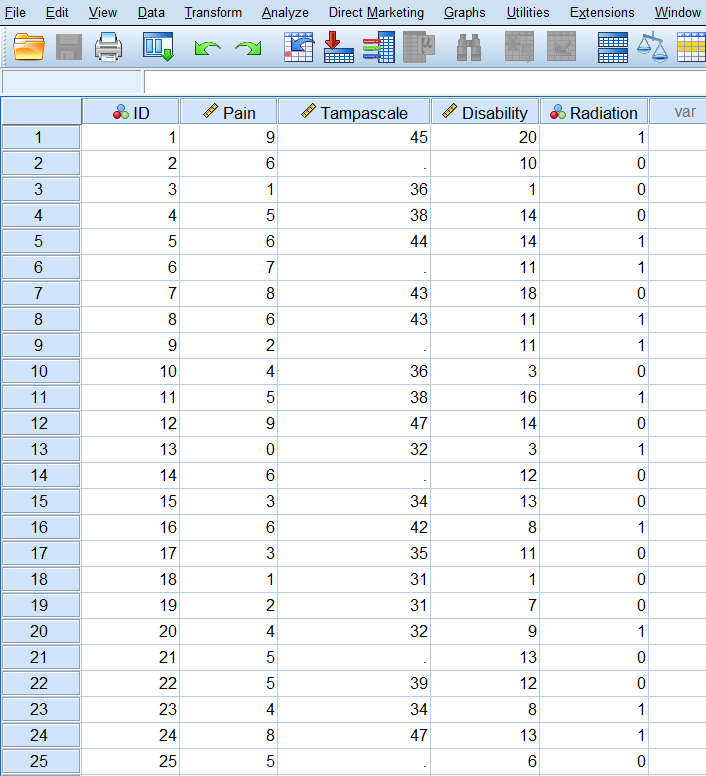
\includegraphics[width=0.95\linewidth]{images/fig1.2} 

}

\caption{Data View window in SPSS}\label{fig:fig2}
\end{figure}

In the lower left corner of the window you can click on the tab Variable
View and the Variable view window will appear (Figure \ref{fig:fig3}).

\begin{figure}

{\centering 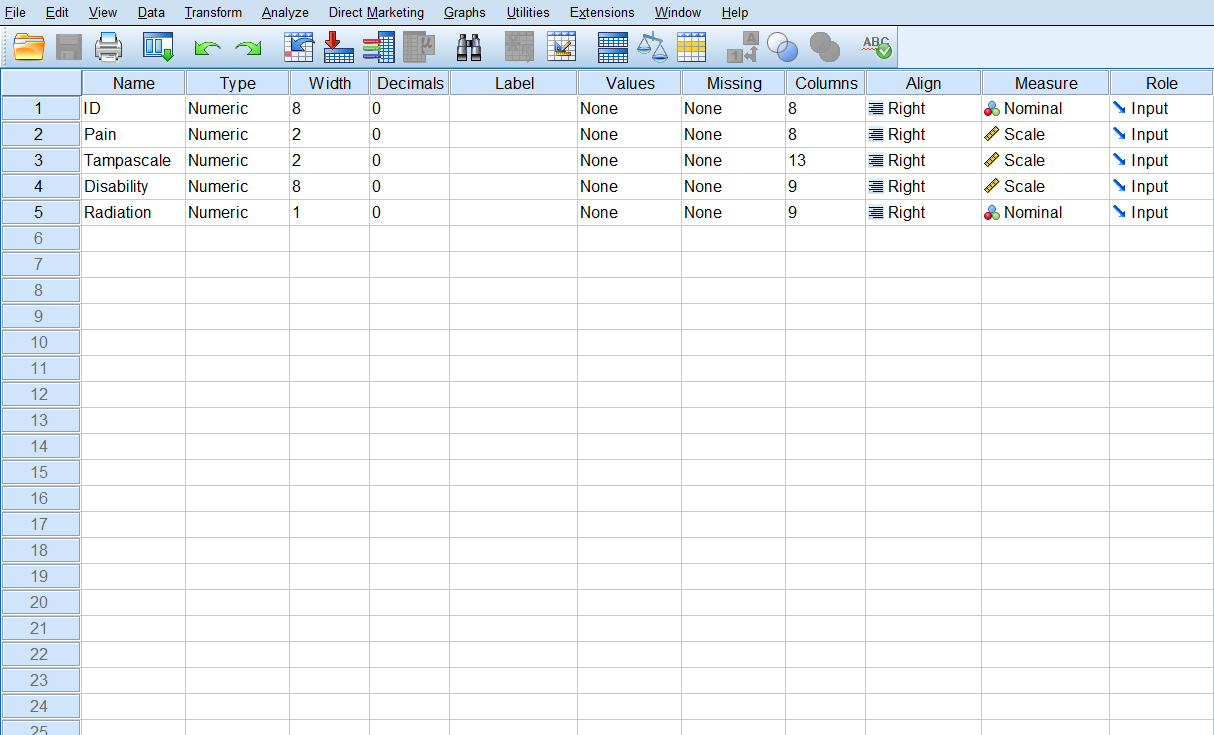
\includegraphics[width=0.95\linewidth]{images/fig1.3} 

}

\caption{Variable View window in SPSS}\label{fig:fig3}
\end{figure}

In the Variable View window, you can add new variables, by entering the
name in the name column. Further, you can change variable options as:
Type: e.g.~numeric or string variable; Width: number of digits;
Decimals: the number of decimal places displayed; Label: add some extra
information about the type of information in the variable; Values: To
assign numbers to the categories of a variable; Missing: you can define
specified data values as user-missing or system missing; Columns: To
change the number of characters displayed in the Data View window;
Align: to specify the alignment of the data; Measure: to specify the
level of each variable, scale (continuous), ordinal or nominal; Role:
Here you can define the role of the variable during your analysis.
Examples are, Input for independent variable, Target for dependent or
outcome variable, Both, independent and dependent variable. There are
more possibilities, but most of the times you use the default Input
setting.

\subsection{Analyzing data in SPSS}\label{analyzing-data-in-spss}

All statistical procedures in SPSS can be found under the Analyze button
(Figure \ref{fig:fig4}). Here you also find the option ``Multiple
Imputation'' which plays an important role in this manual.

\begin{figure}

{\centering 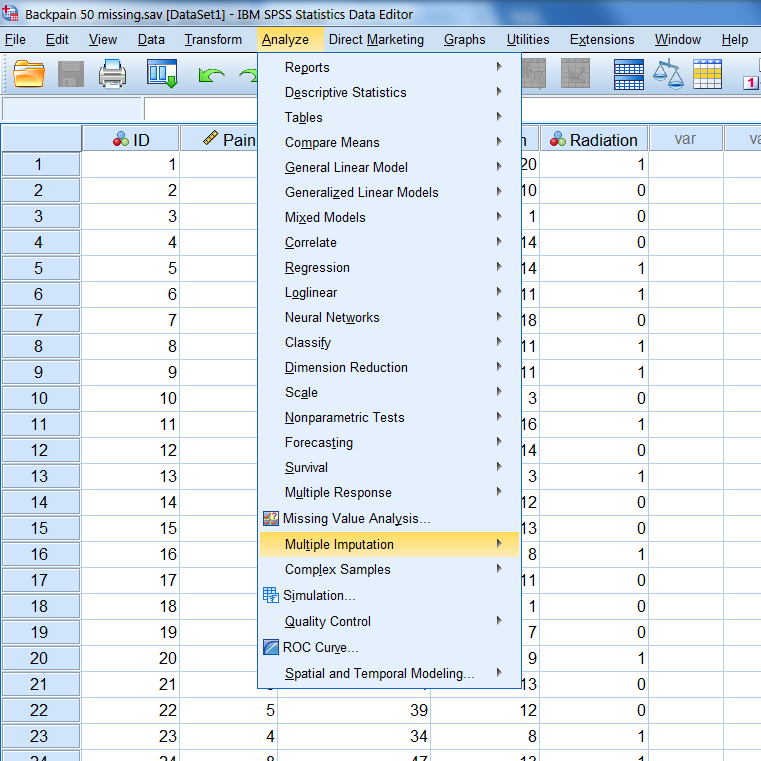
\includegraphics[width=0.95\linewidth]{images/fig1.4} 

}

\caption{Statistical procedures that can be found under the Analyze menu in SPSS}\label{fig:fig4}
\end{figure}

\subsection{The Output window in SPSS}\label{the-output-window-in-spss}

If you have run your analyses in SPSS, an SPSS Output (or viewer) Window
will pop-up. The main body of the Output Window consists of two panes
(left and right panes). In the left pane you find an outline of the
output. In the right pane younfind the actual output of your statistical
procedure (Figure \ref{fig:fig5}).

\begin{figure}

{\centering 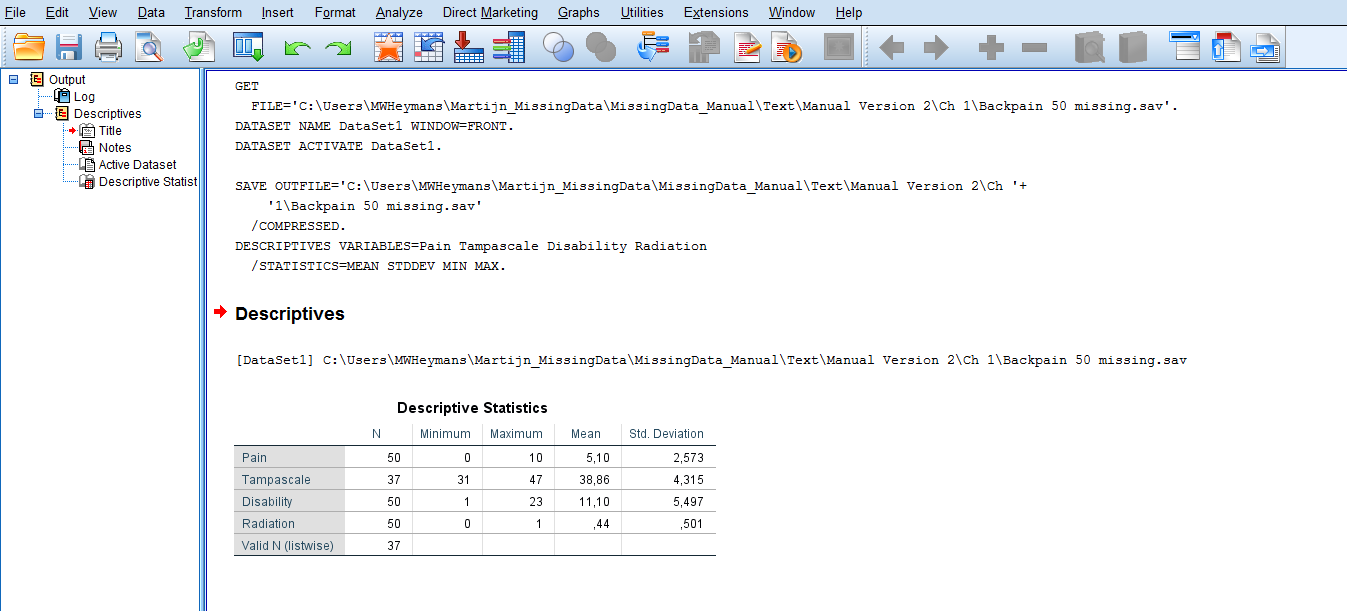
\includegraphics[width=0.95\linewidth]{images/fig1.5} 

}

\caption{Part of the Output or Viewer window in SPSS after making use of Descriptive Statistics under the Analyze menu}\label{fig:fig5}
\end{figure}

\subsection{The Syntax Editor in SPSS}\label{the-syntax-editor-in-spss}

In the syntax editor of SPSS, you use the SPSS syntax programming
language. You can run all SPSS procedures by typing in commands in this
syntax editor window, instead of using the graphical user interface,
i.e.~by using your mouse and clicking on the menu´s. You can get access
to the syntax window in two ways. The first is just by opening a new
syntax file by navigating to

\begin{quote}
File -\textgreater{} New -\textgreater{} Syntax.
\end{quote}

This will open a new syntax window (Figure \ref{fig:fig6}).

\begin{figure}

{\centering 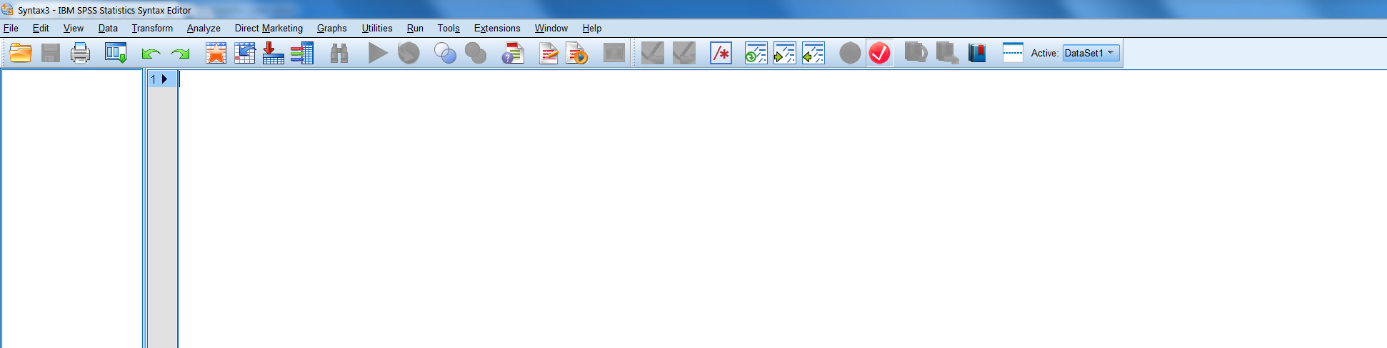
\includegraphics[width=0.95\linewidth]{images/fig1.6} 

}

\caption{Screenshot of new syntax file}\label{fig:fig6}
\end{figure}

You can also generate syntax by accessing statistical procedures through
the dropdown menus and clicking the \texttt{Paste} button instead of
clicking the OK button after you have specified the options. Than a new
Syntax Editor window will pop up or the new syntax will automatically be
added to the open Syntax Editor window. An example can be found in
Figure \ref{fig:fig7}, where the syntax is shown for the Descriptive
Statistics procedure of Figure \ref{fig:fig5}.

\begin{figure}

{\centering 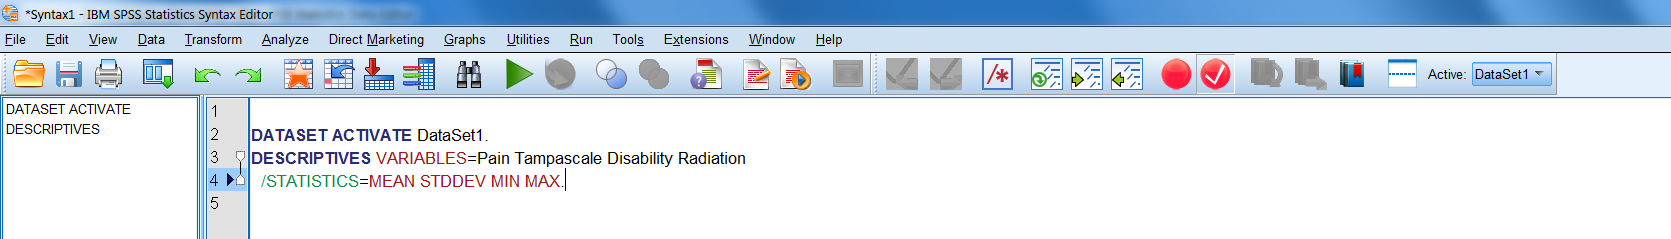
\includegraphics[width=0.95\linewidth]{images/fig1.7} 

}

\caption{Screenshot of Syntax editor of SPSS including the Syntax code for descriptive statisitcs}\label{fig:fig7}
\end{figure}

In this manual we will not use SPSS syntax code to access statistical
procedures. SPSS is most frequently used via the graphical user
interface, and we will use that method also in this manual.

\subsection{Reading and saving data in
SPSS}\label{reading-and-saving-data-in-spss}

You can Read data in, in SPSS via the menu File:

\begin{quote}
File -\textgreater{} Open -\textgreater{} Data.
\end{quote}

All kind of file types can be selected. Of course the SPSS .sav files,
but also .por, .xlsx, .cvs, SAS, Stata, etc. (Figure \ref{fig:fig8})).
After you have selected a specific file type other than SPSS you may
have to go through several steps before you see the data in the Data
View window. These steps are not necessary for SPSS files, they open
directly in the data editor.

\begin{figure}

{\centering 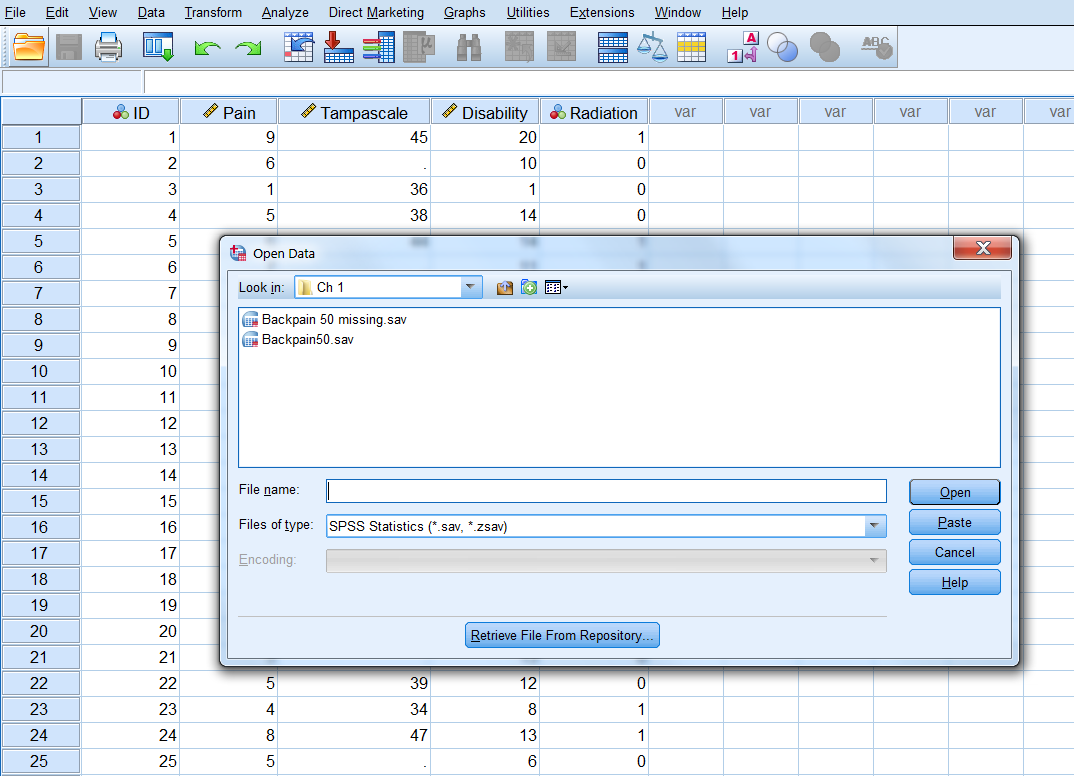
\includegraphics[width=0.95\linewidth]{images/fig1.8} 

}

\caption{Window to read in different file types in SPSS}\label{fig:fig8}
\end{figure}

Saving files in SPSS is possible via the Save Data As option under the
menu File. You can choose the same kind of file types.

\section{R and RStudio}\label{r-and-rstudio}

RStudio is an integrated environment to work with the software program
R. Consequently, to work with RStudio, R has to be installed. RStudio
uses the R language and is also freely available. In this manual we will
show possibilities and options in RStudio that are needed to run the R
code that are discussed in this manual. For more information about
RStudio and its possibilities visit the RStudio website at
www.rstudio.com.

When you open RStudio the following screen will appear.

\begin{figure}

{\centering 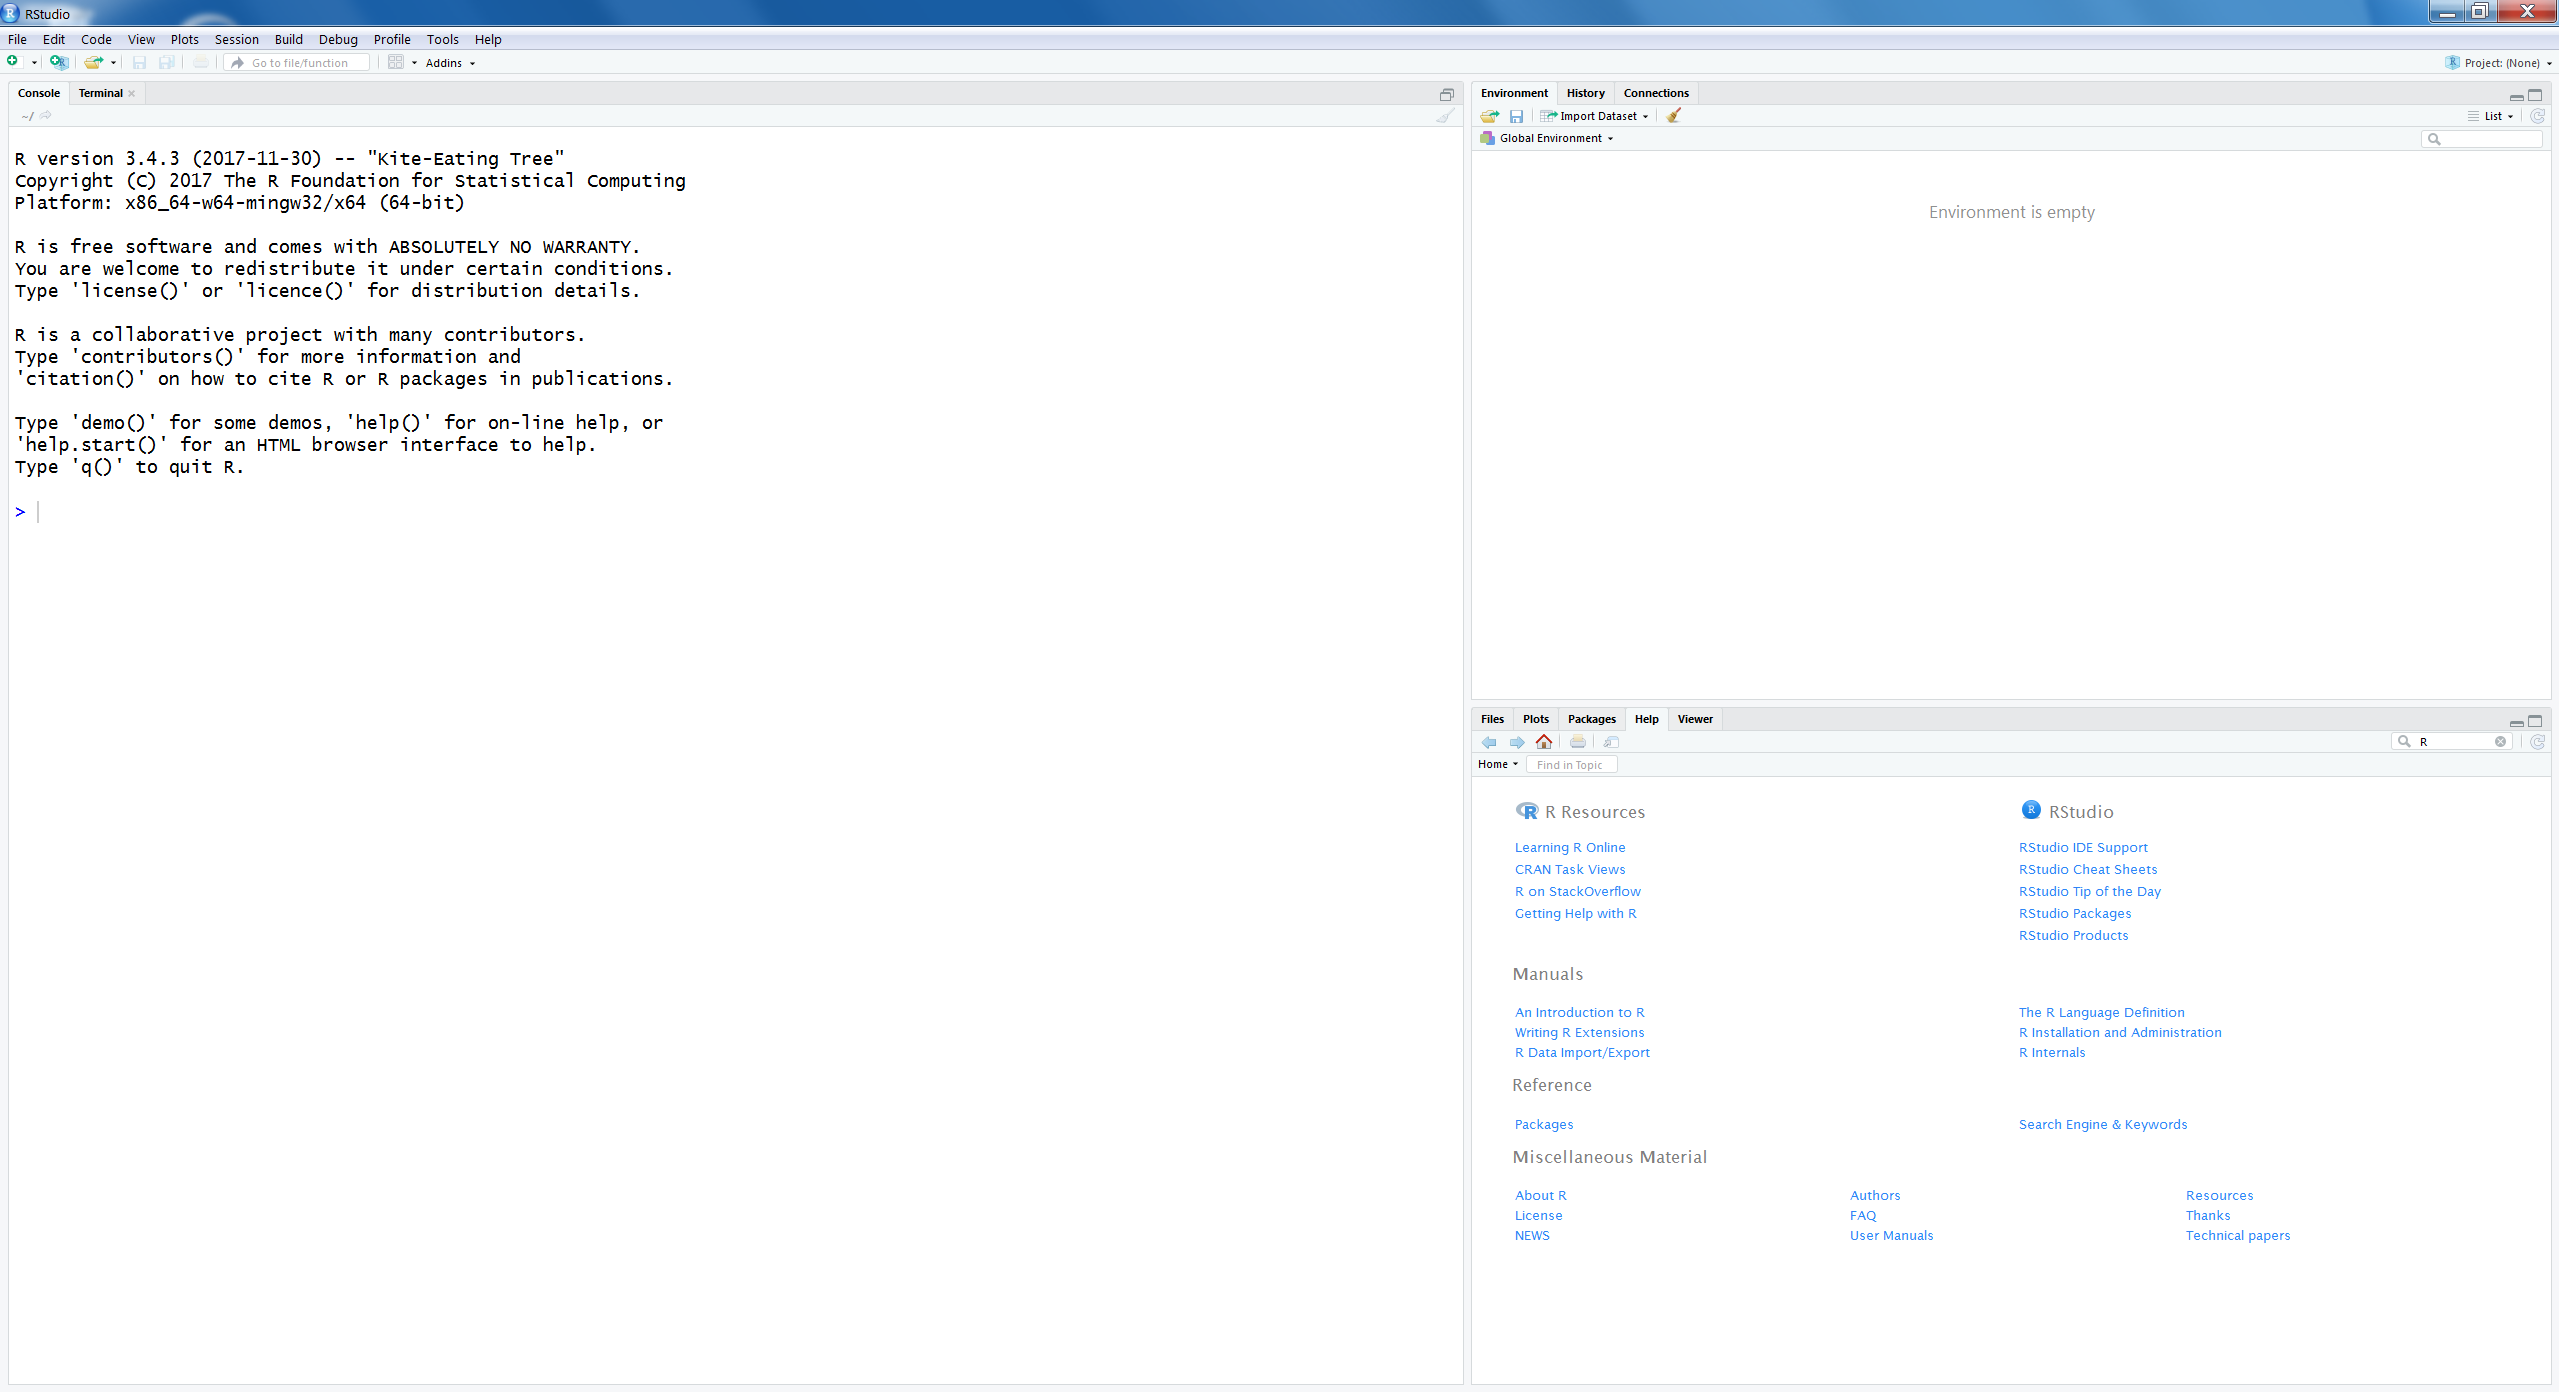
\includegraphics[width=0.95\linewidth]{images/fig1.10} 

}

\caption{First screen that appears after you have started RStudio}\label{fig:fig10}
\end{figure}

There are three windows opened:

\begin{enumerate}
\def\labelenumi{\arabic{enumi}.}
\tightlist
\item
  On the left is the Console window
\end{enumerate}

This is the main window to run R code (see below for more information
about the Console window).

\begin{enumerate}
\def\labelenumi{\arabic{enumi}.}
\setcounter{enumi}{1}
\item
  Right above is the window where you can choose between the Environment
  and History tabs (e.g.~history tracks the code you typed in the
  Console window).
\item
  At the right site below is the window where you can choose between
  Files, Plots, Packages, Help and Viewer tabs.
\end{enumerate}

\subsection{The role of the Console
Window}\label{the-role-of-the-console-window}

When you enter code in the Console window you will directly receive a
result. For example, when you type 3 + 3 the result will appear
directly.

\begin{Shaded}
\begin{Highlighting}[]
\DecValTok{3} \OperatorTok{+}\StringTok{ }\DecValTok{3}
\end{Highlighting}
\end{Shaded}

\begin{verbatim}
## [1] 6
\end{verbatim}

Other multiplication procedures as divide, square, etc. can also be
executed. The main use for R is its functions. For example, to generate
20 random numbers you use the following function code (we will discuss
more about functions in R later):

\begin{Shaded}
\begin{Highlighting}[]
\KeywordTok{rnorm}\NormalTok{(}\DecValTok{20}\NormalTok{)}
\end{Highlighting}
\end{Shaded}

\begin{verbatim}
##  [1] -0.77630271 -0.49168125  1.16571862 -0.26507526  0.83691937
##  [6]  1.41193609  0.51484941 -1.31591819 -1.90453560  1.69929682
## [11] -0.18813274  0.62318790  0.09096109  0.48229074 -1.05643562
## [16] -1.13726685  1.08547710 -0.51094522  1.11487616  1.51544921
\end{verbatim}

The number {[}1{]} between brackets is the index of the first number or
item in the vector.

\subsection{R assignments and objects}\label{r-assignments-and-objects}

In R it is possible to create objects and to assign values to these
objects. In this way it is possible to store some intermediate results
and recall or use them later on. Assigning values to objects is done by
using the assignment operator \textless{}- . You can also use the = sign
as an assignment operator. This is not recommended because this is also
a symbol used for mathematical operations. For example, when we want to
assign the value 3 to the object x, we use:

\begin{Shaded}
\begin{Highlighting}[]
\NormalTok{x <-}\StringTok{ }\DecValTok{3} 
\end{Highlighting}
\end{Shaded}

When we subsequently type in the letter x we get the following result:

\begin{Shaded}
\begin{Highlighting}[]
\NormalTok{x }
\end{Highlighting}
\end{Shaded}

\begin{verbatim}
## [1] 3
\end{verbatim}

Now the value 3 is assigned to the object x. In R all kind of
information can be assigned to an object, i.e.~one number, a vector of
numbers, results from analysis or other R objects such as data frames,
matrices or lists. Objects can have all kinds of different names,
composed of different letters and numbers. Here are some examples where
number 3 is assigned to different objects with different names:

\begin{Shaded}
\begin{Highlighting}[]
\NormalTok{test <-}\StringTok{ }\DecValTok{3}
\NormalTok{test.}\DecValTok{1}\NormalTok{ <-}\StringTok{ }\DecValTok{3}
\NormalTok{test.manual <-}\StringTok{ }\DecValTok{3}
\NormalTok{test}
\end{Highlighting}
\end{Shaded}

\begin{verbatim}
## [1] 3
\end{verbatim}

\begin{Shaded}
\begin{Highlighting}[]
\NormalTok{test.}\DecValTok{1}
\end{Highlighting}
\end{Shaded}

\begin{verbatim}
## [1] 3
\end{verbatim}

\begin{Shaded}
\begin{Highlighting}[]
\NormalTok{test.manual }
\end{Highlighting}
\end{Shaded}

\begin{verbatim}
## [1] 3
\end{verbatim}

Note that some letters and words are used by R itself. It is not
recommended to use these leters as names for objects in R that you
create yourself. For example, the letter T and F are used as TRUE and
FALSE by R. Other letters that are already in use are c, q, t, C, D, I
and diff, df, and pt.

\subsection{Vectors, matrices, lists and data
frames}\label{vectors-matrices-lists-and-data-frames}

\textbf{Vectors}

A vector can be created by the following code:

\begin{Shaded}
\begin{Highlighting}[]
\NormalTok{y <-}\StringTok{ }\KeywordTok{c}\NormalTok{(}\DecValTok{1}\NormalTok{, }\DecValTok{2}\NormalTok{, }\DecValTok{3}\NormalTok{, }\DecValTok{4}\NormalTok{, }\DecValTok{5}\NormalTok{)}
\NormalTok{y}
\end{Highlighting}
\end{Shaded}

\begin{verbatim}
## [1] 1 2 3 4 5
\end{verbatim}

The numbers 1, 2, 3, 4 and 5 are assigned to the data vector y. The
``c'' in the above code stand for concatenate which makes that all
separate (one-vector) numbers are merged into one vector. It is also
possible to create character vectors, which are vectors that contain
strings (text). An example:

\begin{Shaded}
\begin{Highlighting}[]
\NormalTok{y <-}\StringTok{ }\KeywordTok{c}\NormalTok{(}\StringTok{"a"}\NormalTok{, }\StringTok{"b"}\NormalTok{, }\StringTok{"test"}\NormalTok{)}
\NormalTok{y}
\end{Highlighting}
\end{Shaded}

\begin{verbatim}
## [1] "a"    "b"    "test"
\end{verbatim}

Vectors can also be made by using the ``:'' symbol. With that symbol it
is easy to generate a sequence of numbers. An example:

\begin{Shaded}
\begin{Highlighting}[]
\NormalTok{y <-}\StringTok{ }\DecValTok{1}\OperatorTok{:}\DecValTok{10}
\NormalTok{y}
\end{Highlighting}
\end{Shaded}

\begin{verbatim}
##  [1]  1  2  3  4  5  6  7  8  9 10
\end{verbatim}

\textbf{Matrix}

You can create a matrix by using the matrix function.

\begin{Shaded}
\begin{Highlighting}[]
\KeywordTok{matrix}\NormalTok{(}\KeywordTok{c}\NormalTok{(}\DecValTok{1}\NormalTok{, }\DecValTok{2}\NormalTok{, }\DecValTok{3}\NormalTok{, }\DecValTok{4}\NormalTok{, }\DecValTok{5}\NormalTok{, }\DecValTok{6}\NormalTok{), }\DataTypeTok{nrow=}\DecValTok{2}\NormalTok{, }\DataTypeTok{ncol=}\DecValTok{3}\NormalTok{)}
\end{Highlighting}
\end{Shaded}

\begin{verbatim}
##      [,1] [,2] [,3]
## [1,]    1    3    5
## [2,]    2    4    6
\end{verbatim}

Now we have created a matrix with 2 rows and 3 columns. In essence we
converted the vector c(1, 2, 3, 4, 5, 6) into a matrix.

\textbf{List}

Another object is called a list. A list can contain components of
different formats. Let's look at an example using the following code:

\begin{Shaded}
\begin{Highlighting}[]
\NormalTok{x <-}\StringTok{ }\DecValTok{1}\OperatorTok{:}\DecValTok{5}
\NormalTok{x}
\end{Highlighting}
\end{Shaded}

\begin{verbatim}
## [1] 1 2 3 4 5
\end{verbatim}

\begin{Shaded}
\begin{Highlighting}[]
\NormalTok{y <-}\StringTok{ }\KeywordTok{c}\NormalTok{(}\StringTok{"a"}\NormalTok{, }\StringTok{"b"}\NormalTok{, }\StringTok{"test"}\NormalTok{)}
\NormalTok{z <-}\StringTok{ }\KeywordTok{list}\NormalTok{(}\DataTypeTok{x=}\NormalTok{x, }\DataTypeTok{y=}\NormalTok{y)}
\NormalTok{z}
\end{Highlighting}
\end{Shaded}

\begin{verbatim}
## $x
## [1] 1 2 3 4 5
## 
## $y
## [1] "a"    "b"    "test"
\end{verbatim}

With this code you created the list object z consisting of the two
components x and y which are the vectors that were created above. You
see that in a list two components of different data type can be
combined, a numeric and a character factor. The names of the list
components are indicated by the dollar sign, \texttt{\$}. The list
component can be obtained separately by typing \texttt{z\$x} for
component x or \texttt{x\$y} for component y.

\textbf{Dataframe}

Mostly we work with datasets that contain information of different
variables and persons. In R such a dataset is called a dataframe.
Typically, a dataframe is created by reading in an existing dataset. How
to create a dataframe by reading in a dataset will be further discussed
in the paragraph ``Reading in and saving data''.

\subsection{Indexing Vectors, Matrices, Lists and Data
frames}\label{indexing-vectors-matrices-lists-and-data-frames}

\textbf{Vectors}

An important operation in R is to select a subset of elements of a given
vector. This is called indexing vectors. This subset can be assigned to
another vector. For example:

\begin{Shaded}
\begin{Highlighting}[]
\NormalTok{y <-}\StringTok{ }\KeywordTok{c}\NormalTok{(}\DecValTok{3}\NormalTok{, }\DecValTok{5}\NormalTok{, }\DecValTok{2}\NormalTok{, }\DecValTok{8}\NormalTok{, }\DecValTok{5}\NormalTok{, }\DecValTok{4}\NormalTok{, }\DecValTok{8}\NormalTok{, }\DecValTok{1}\NormalTok{, }\DecValTok{3}\NormalTok{, }\DecValTok{6}\NormalTok{)}
\NormalTok{y[}\KeywordTok{c}\NormalTok{(}\DecValTok{1}\NormalTok{, }\DecValTok{4}\NormalTok{)]}
\end{Highlighting}
\end{Shaded}

\begin{verbatim}
## [1] 3 8
\end{verbatim}

The R code y{[}c(1, 4){]}, extracts the first and fourth element of the
vector. Another example is by using the ``:'' symbol, to extract several
subsequent elements:

\begin{Shaded}
\begin{Highlighting}[]
\NormalTok{y[}\DecValTok{2}\OperatorTok{:}\DecValTok{5}\NormalTok{]}
\end{Highlighting}
\end{Shaded}

\begin{verbatim}
## [1] 5 2 8 5
\end{verbatim}

The R code y{[}2:5{]}, extracts the second to the fifth element of the
vector.

A minus sign excludes the specific element from the vector, like:

\begin{Shaded}
\begin{Highlighting}[]
\NormalTok{y[}\OperatorTok{-}\DecValTok{3}\NormalTok{]}
\end{Highlighting}
\end{Shaded}

\begin{verbatim}
## [1] 3 5 8 5 4 8 1 3 6
\end{verbatim}

The R code y{[}-3{]}, excludes the third element of the vector (i.e.~2).
A new vector z can be created where the third and fourth element of the
y vector are excluded:

\begin{Shaded}
\begin{Highlighting}[]
\NormalTok{z <-}\StringTok{ }\NormalTok{y[}\OperatorTok{-}\KeywordTok{c}\NormalTok{(}\DecValTok{3}\NormalTok{, }\DecValTok{4}\NormalTok{)]}
\NormalTok{z}
\end{Highlighting}
\end{Shaded}

\begin{verbatim}
## [1] 3 5 5 4 8 1 3 6
\end{verbatim}

\textbf{Matrices}

When we index matrices we can choose to index rows, columns or both.
Here are some examples:

First construct the matrix z:

\begin{Shaded}
\begin{Highlighting}[]
\NormalTok{z <-}\StringTok{ }\KeywordTok{matrix}\NormalTok{(}\DecValTok{1}\OperatorTok{:}\DecValTok{9}\NormalTok{, }\DataTypeTok{nrow=}\DecValTok{3}\NormalTok{)}
\NormalTok{z}
\end{Highlighting}
\end{Shaded}

\begin{verbatim}
##      [,1] [,2] [,3]
## [1,]    1    4    7
## [2,]    2    5    8
## [3,]    3    6    9
\end{verbatim}

Extract from the first row the number in the second column

\begin{Shaded}
\begin{Highlighting}[]
\NormalTok{z[}\DecValTok{1}\NormalTok{, }\DecValTok{2}\NormalTok{]}
\end{Highlighting}
\end{Shaded}

\begin{verbatim}
## [1] 4
\end{verbatim}

Extract all numbers in each column in the first row

\begin{Shaded}
\begin{Highlighting}[]
\NormalTok{z[}\DecValTok{1}\NormalTok{, ]}
\end{Highlighting}
\end{Shaded}

\begin{verbatim}
## [1] 1 4 7
\end{verbatim}

Extract all numbers in each row of the first column

\begin{Shaded}
\begin{Highlighting}[]
\NormalTok{z[, }\DecValTok{1}\NormalTok{]}
\end{Highlighting}
\end{Shaded}

\begin{verbatim}
## [1] 1 2 3
\end{verbatim}

A minus sign can also be used to delete specific elements or complete
rows or columns.

You can omit the first row from the matrix z

\begin{Shaded}
\begin{Highlighting}[]
\NormalTok{z[}\OperatorTok{-}\DecValTok{1}\NormalTok{, ]}
\end{Highlighting}
\end{Shaded}

\begin{verbatim}
##      [,1] [,2] [,3]
## [1,]    2    5    8
## [2,]    3    6    9
\end{verbatim}

\textbf{Lists}

First create a list with 3 components, each component consists of a
vector of the same length and with 10 elements each.

\begin{Shaded}
\begin{Highlighting}[]
\NormalTok{k <-}\StringTok{ }\KeywordTok{list}\NormalTok{(}\DataTypeTok{a=}\DecValTok{1}\OperatorTok{:}\DecValTok{10}\NormalTok{, }\DataTypeTok{b=}\DecValTok{11}\OperatorTok{:}\DecValTok{20}\NormalTok{, }\DataTypeTok{c=}\DecValTok{21}\OperatorTok{:}\DecValTok{30}\NormalTok{)}
\NormalTok{k}
\end{Highlighting}
\end{Shaded}

\begin{verbatim}
## $a
##  [1]  1  2  3  4  5  6  7  8  9 10
## 
## $b
##  [1] 11 12 13 14 15 16 17 18 19 20
## 
## $c
##  [1] 21 22 23 24 25 26 27 28 29 30
\end{verbatim}

Index the individual component b by using the following code:

\begin{Shaded}
\begin{Highlighting}[]
\NormalTok{k}\OperatorTok{$}\NormalTok{b}
\end{Highlighting}
\end{Shaded}

\begin{verbatim}
##  [1] 11 12 13 14 15 16 17 18 19 20
\end{verbatim}

\begin{Shaded}
\begin{Highlighting}[]
\NormalTok{k[[}\StringTok{"b"}\NormalTok{]]}
\end{Highlighting}
\end{Shaded}

\begin{verbatim}
##  [1] 11 12 13 14 15 16 17 18 19 20
\end{verbatim}

\begin{Shaded}
\begin{Highlighting}[]
\NormalTok{k[[}\DecValTok{2}\NormalTok{]]}
\end{Highlighting}
\end{Shaded}

\begin{verbatim}
##  [1] 11 12 13 14 15 16 17 18 19 20
\end{verbatim}

To extract individual list components double square brackets are used,
compared to single brackets for indexing vectors and matrices.

When you use single brackets, you get the following results:

\begin{Shaded}
\begin{Highlighting}[]
\NormalTok{k[}\StringTok{"b"}\NormalTok{]}
\end{Highlighting}
\end{Shaded}

\begin{verbatim}
## $b
##  [1] 11 12 13 14 15 16 17 18 19 20
\end{verbatim}

The difference between using single and double brackets is that single
brackets return the component data type, which is in this case a vector
(but could be any kind of data type) and single brackets always return a
list.

\textbf{Data frames}

Indexing data frames follows the same method as indexing matrices, but
we can also use the method that is used to index lists, since data
frames are essentially lists of vectors of the same length. Data frames
consist of rows and columns which can be accessed separately or both to
extract specific elements. We use the data frame that was constructed in
R code 1.11.

\begin{Shaded}
\begin{Highlighting}[]
\NormalTok{z}
\end{Highlighting}
\end{Shaded}

\begin{verbatim}
##      [,1] [,2] [,3]
## [1,]    1    4    7
## [2,]    2    5    8
## [3,]    3    6    9
\end{verbatim}

To index the first column you use:

\begin{Shaded}
\begin{Highlighting}[]
\NormalTok{z[, }\DecValTok{1}\NormalTok{]}
\end{Highlighting}
\end{Shaded}

\begin{verbatim}
## [1] 1 2 3
\end{verbatim}

\begin{Shaded}
\begin{Highlighting}[]
\NormalTok{k}\OperatorTok{$}\NormalTok{a}
\end{Highlighting}
\end{Shaded}

\begin{verbatim}
##  [1]  1  2  3  4  5  6  7  8  9 10
\end{verbatim}

The second row can be accessed by using:

\begin{Shaded}
\begin{Highlighting}[]
\NormalTok{z[}\DecValTok{2}\NormalTok{, ]}
\end{Highlighting}
\end{Shaded}

\begin{verbatim}
## [1] 2 5 8
\end{verbatim}

\subsection{Vectorized Calculation}\label{vectorized-calculation}

With R it is possible to perform vectorized calculations. This means
that you can do calculations elementwise, i.e.~the same calculation is
done on each element of an object. Let's look at an example.

First create a vector z with numerical variables.

\begin{Shaded}
\begin{Highlighting}[]
\NormalTok{z <-}\StringTok{ }\KeywordTok{c}\NormalTok{(}\DecValTok{1}\NormalTok{, }\DecValTok{2}\NormalTok{, }\DecValTok{3}\NormalTok{, }\DecValTok{4}\NormalTok{, }\DecValTok{5}\NormalTok{, }\DecValTok{6}\NormalTok{, }\DecValTok{7}\NormalTok{, }\DecValTok{8}\NormalTok{)}
\NormalTok{z}
\end{Highlighting}
\end{Shaded}

\begin{verbatim}
## [1] 1 2 3 4 5 6 7 8
\end{verbatim}

Now you can fairly easy square each element of the vector by typing:

\begin{Shaded}
\begin{Highlighting}[]
\NormalTok{z}\OperatorTok{^}\DecValTok{2}
\end{Highlighting}
\end{Shaded}

\begin{verbatim}
## [1]  1  4  9 16 25 36 49 64
\end{verbatim}

We see that each element is squared. You can do these vectorized
calculations by using all kinds of mathematical functions, e.g.~taking
the square root, logarithms, adding constant values to each element,
etc.

\subsection{R Functions}\label{r-functions}

Functions play an important role in R. Functions can be seen as lines of
R code to run all kind of data procedures and to return a result. Take
for example the small function ``print.sum.test'' that generates a
sequence of numbers from 1 to 5 and sums all values from 1 to the value
we define beforehand, which is here the value 3. This means that the
function will sum all values from 1 to 3, i.e.~1 + 2 + 3 when it is at
the value of 3 and all values from 1 to 4 when we use as input value the
value 4.

\begin{Shaded}
\begin{Highlighting}[]
\NormalTok{print.sum.test <-}\StringTok{ }\ControlFlowTok{function}\NormalTok{(x) }
\NormalTok{\{}
 \ControlFlowTok{for}\NormalTok{ (i }\ControlFlowTok{in} \DecValTok{1}\OperatorTok{:}\DecValTok{5}\NormalTok{) }
\NormalTok{ \{}
   \ControlFlowTok{if}\NormalTok{ (i}\OperatorTok{==}\NormalTok{x) y <-}\StringTok{ }\KeywordTok{sum}\NormalTok{(}\DecValTok{1}\OperatorTok{:}\NormalTok{i)  }
\NormalTok{ \}}
\KeywordTok{return}\NormalTok{(y)}
\NormalTok{\}}
\KeywordTok{print.sum.test}\NormalTok{(}\DecValTok{3}\NormalTok{)}
\end{Highlighting}
\end{Shaded}

\begin{verbatim}
## [1] 6
\end{verbatim}

At the first line we define the function print.sum.test that includes
one argument x. Than in de body of the function which starts with a left
brace and ends with another brace, the actual calculations take place.
The return statement gives back the result. At the end we call the
function with the statement print.sum.test(3), where the value 3 is
actually used in the function.

Once the function is defined, you can call the function and plug in
other values. For example:

\begin{Shaded}
\begin{Highlighting}[]
\KeywordTok{print.sum.test}\NormalTok{(}\DecValTok{4}\NormalTok{)}
\end{Highlighting}
\end{Shaded}

\begin{verbatim}
## [1] 10
\end{verbatim}

You can write functions yourself but in R many functions are available
which means that many calculations are done by using function calls. A
function name is followed by a set of parentheses which contain some
arguments. In the above self-written function, we already made use of a
function, which is the sum function. We can use it separately as
follows:

\begin{Shaded}
\begin{Highlighting}[]
\KeywordTok{sum}\NormalTok{(}\DecValTok{3}\NormalTok{,}\DecValTok{4}\NormalTok{)}
\end{Highlighting}
\end{Shaded}

\begin{verbatim}
## [1] 7
\end{verbatim}

The arguments in this function are the numbers 3 and 4 and the result is
their sum. This function uses as arguments numbers or complete vectors.

If you want to see the formal arguments of each function you can use the
args function. For example, you can use it for the matrix function:

\begin{Shaded}
\begin{Highlighting}[]
\KeywordTok{args}\NormalTok{(matrix)}
\end{Highlighting}
\end{Shaded}

\begin{verbatim}
## function (data = NA, nrow = 1, ncol = 1, byrow = FALSE, dimnames = NULL) 
## NULL
\end{verbatim}

As a result the arguments of the functions are listed with their default
settings. In this case the arguments are:

data: an optional data vector (including a list or expression vector).

nrow: the desired number of rows.

ncol: the desired number of columns.

byrow: logical. If FALSE (the default) the matrix is filled by columns,
otherwise the matrix is filled by rows.

dimnames: A dimnames attribute for the matrix: NULL or a list of length
2 giving the row and column names respectively. An empty list is treated
as NULL, and a list of length one as row names. The list can be named,
and the list names will be used as names for the dimensions.

\subsection{The Help function}\label{the-help-function}

There are several possibilities to start the help facilities in R and to
get more information about functions and their arguments in R.

You can just type help or use the question mark as follows:

\begin{Shaded}
\begin{Highlighting}[]
\KeywordTok{help}\NormalTok{(matrix)}
\NormalTok{?matrix}
\end{Highlighting}
\end{Shaded}

In both ways the help tutorial for the matrix function will be activated
and appear in your web browser or in help tab in the right corner below
when you use R studio.

\subsection{Working with script files}\label{working-with-script-files}

If you want to use R code and functions more than once it is useful to
work with scripts files. In this way you can type and save R code and
reuse it. To create a script file in R is easy.

After you have started RStudio you go to

\begin{quote}
File -\textgreater{} New File -\textgreater{} R Scripts
\end{quote}

A new window will open on the left side above. In that file you can type
for example the self-written function print.sum.test. (Figure
\ref{fig:fig11}). You can save the script file by using the Save option
under the File menu, open it again and use it whenever you want.

\begin{figure}

{\centering 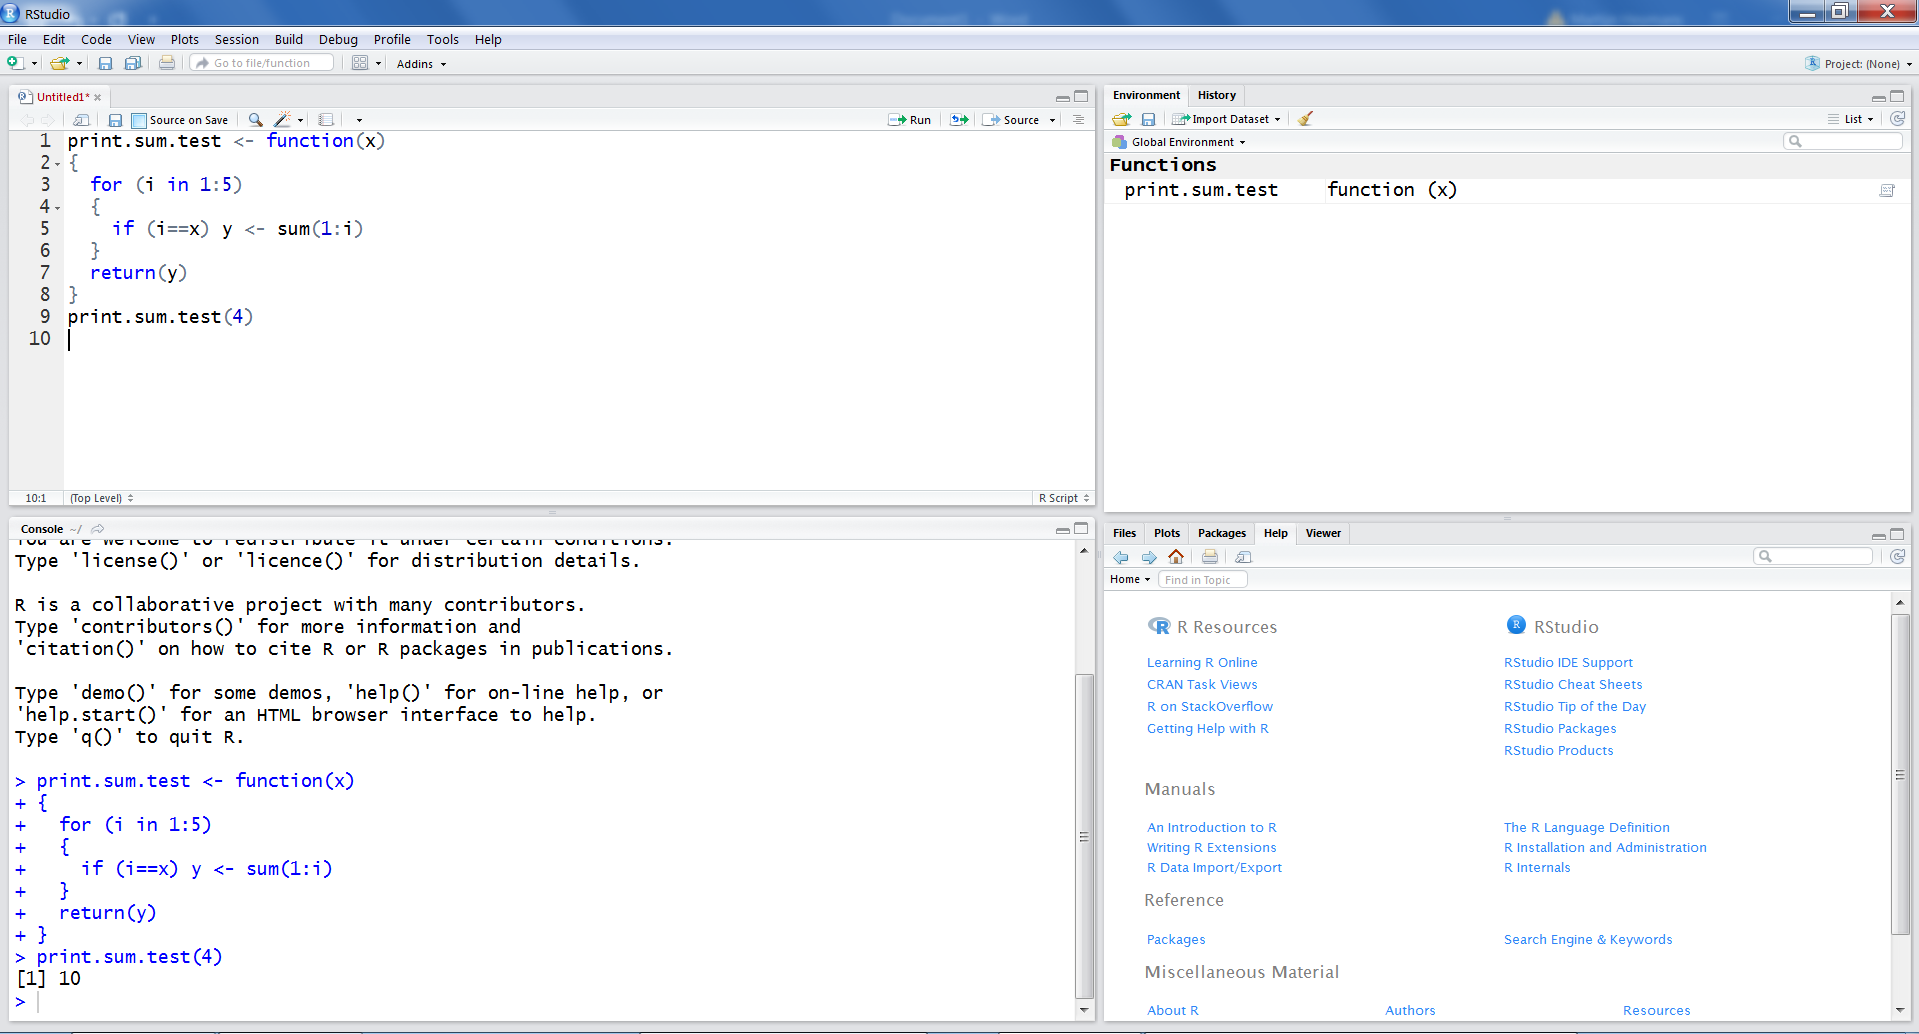
\includegraphics[width=0.95\linewidth]{images/fig1.11} 

}

\caption{Script file example in RStudio}\label{fig:fig11}
\end{figure}

\subsection{Creating a working
directory}\label{creating-a-working-directory}

It is a good idea to keep your R files at the same place when you are
doing data analysis for some kind of project. If you do not use a
separate directory, R will use a default directory, that will mostly be
in Windows in the documents folder. All files that you have to use or
save during your R session are in that directory. To locate your working
directory, you can type in the Console window:

\begin{Shaded}
\begin{Highlighting}[]
\KeywordTok{getwd}\NormalTok{()}
\end{Highlighting}
\end{Shaded}

You can change the working directory in another way. Go in RStudio to
the window on the right site below and go to the Files tab and click on
the right site of the screen on the three dots. Than a window will open
and you can browse to your preferred folder. Then choose for More in the
Files tab and then select ``Set As Working Directory'' (Figure
\ref{fig:fig12}). Now you have set your preferred working directory. You
can check if your directory is set correctly by choosing ``Go To Working
Directory''.

\begin{figure}

{\centering 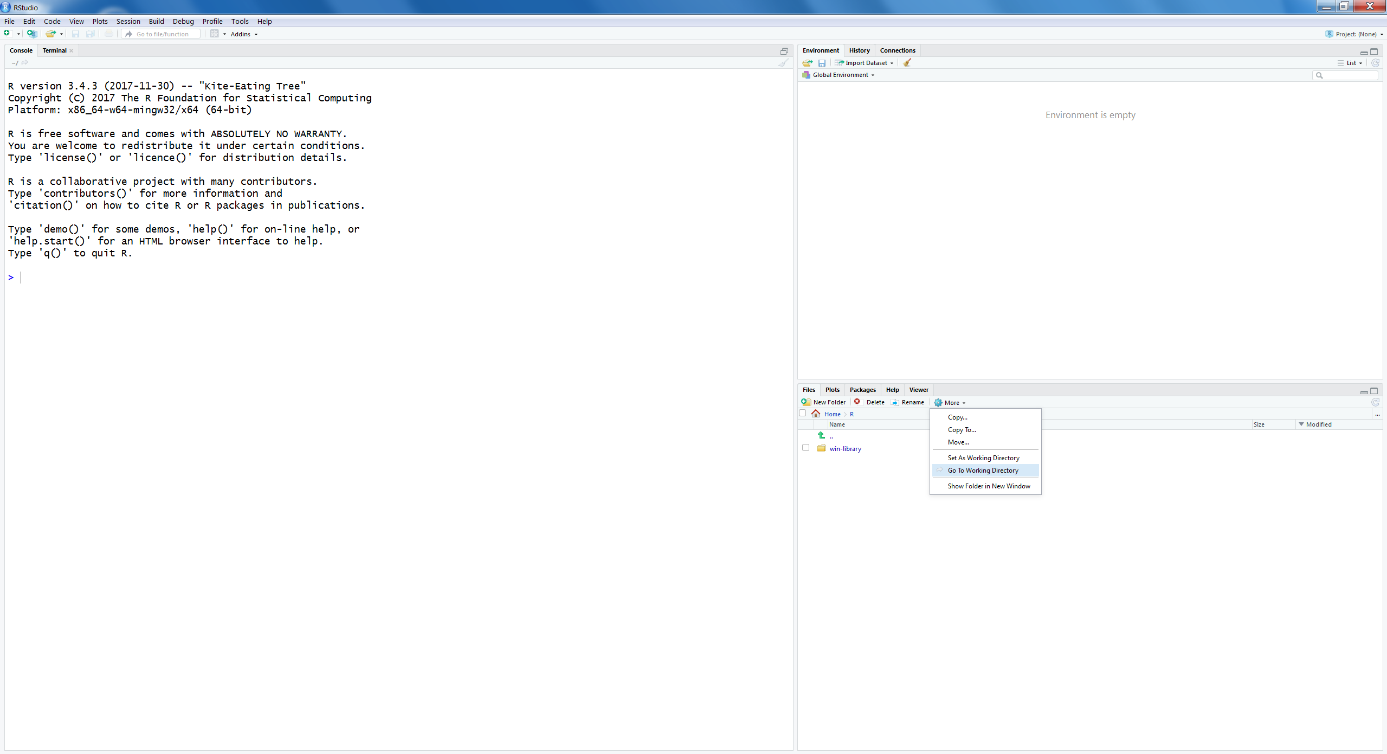
\includegraphics[width=0.95\linewidth]{images/fig1.12} 

}

\caption{Working directory selection in RStudio}\label{fig:fig12}
\end{figure}

\subsection{Reading in SPSS data in
RStudio}\label{reading-in-spss-data-in-rstudio}

There are several procedures in RStudio to read in datasets.

\begin{enumerate}
\def\labelenumi{\arabic{enumi}.}
\tightlist
\item
  Import datasets via ``Import Dataset''
\end{enumerate}

An easy way is via the window at the right site above. There you will
find the button ``Import Dataset''. When you click on it you can choose
between different kind of file types, i.e.~CVS, Excel, SPSS, SAS and
Stata files (Figure \ref{fig:fig13})).

\begin{figure}

{\centering 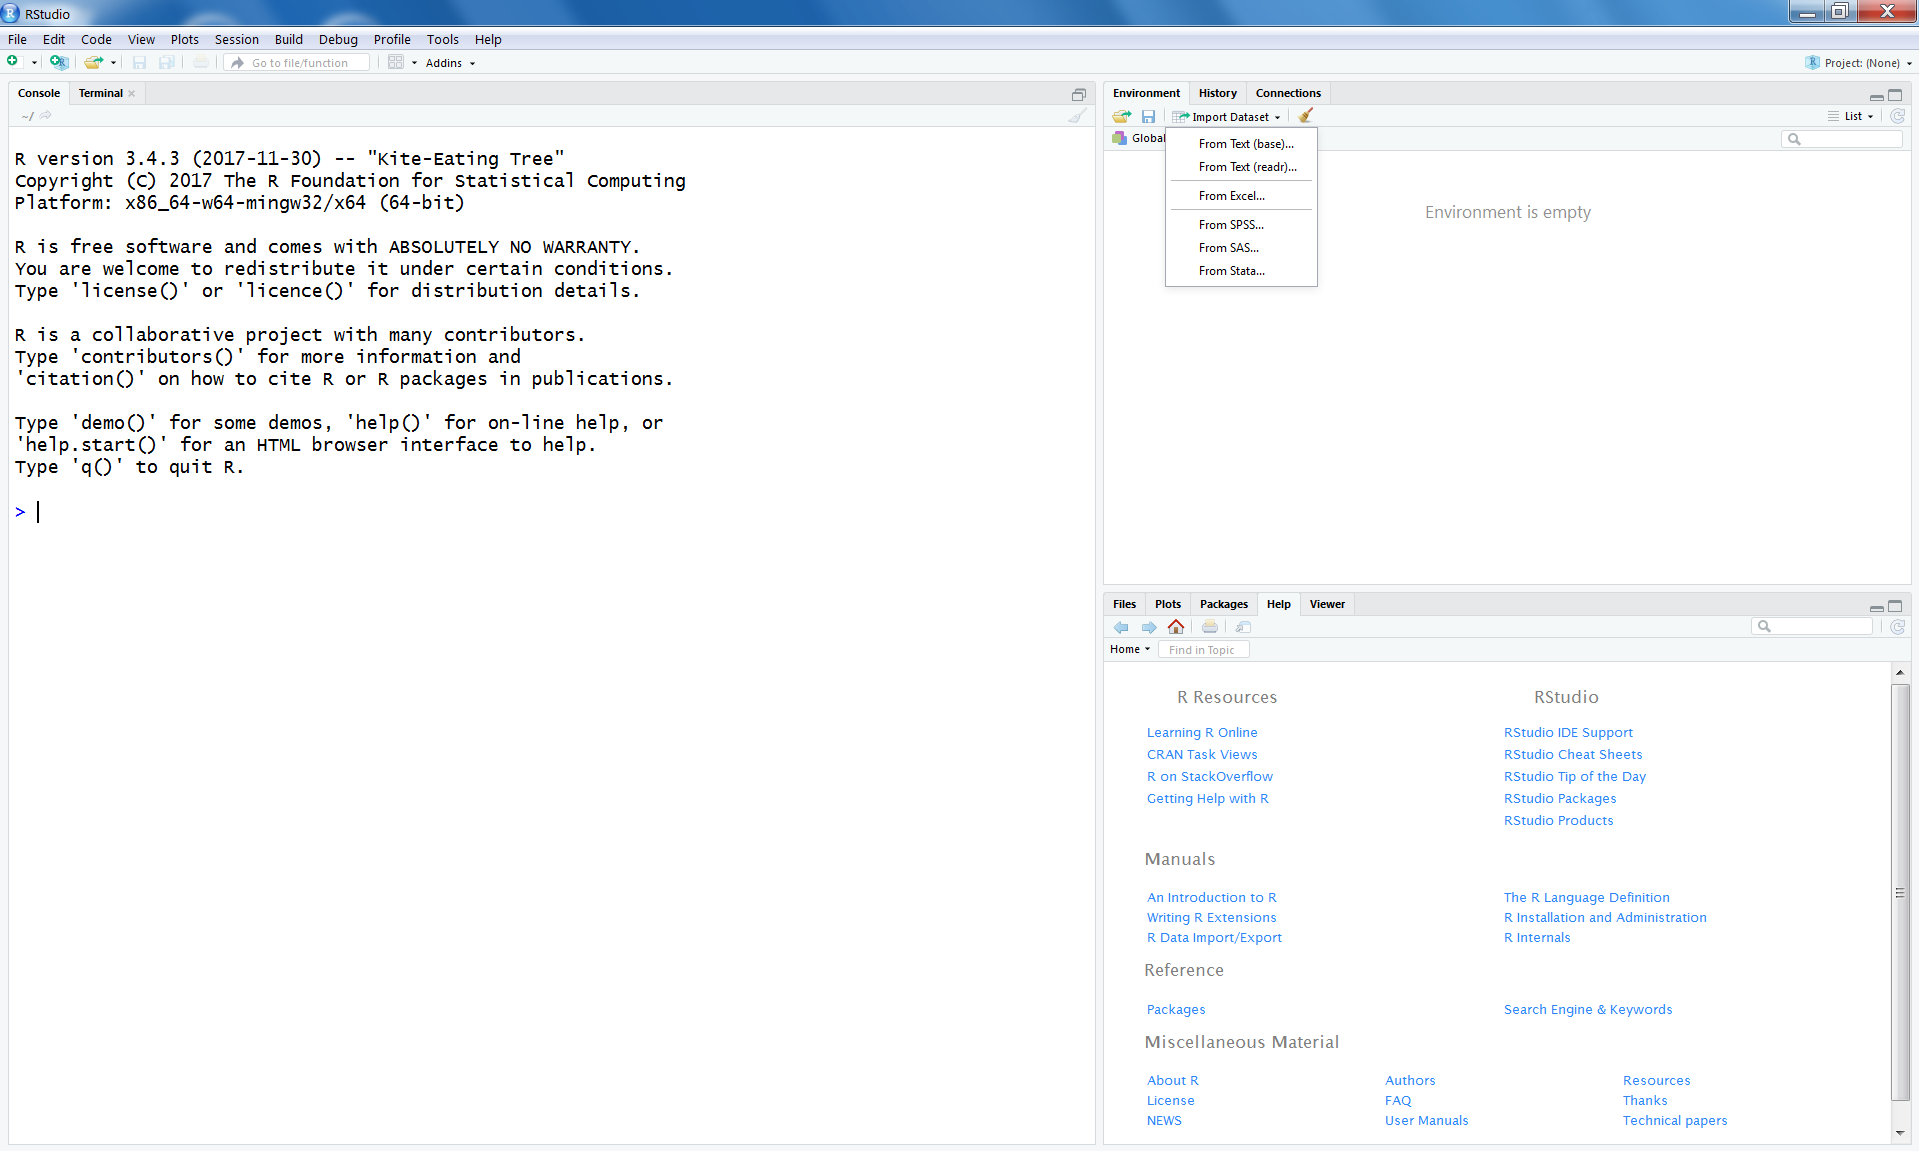
\includegraphics[width=0.95\linewidth]{images/fig1.13} 

}

\caption{Screen to import datasets in RStudio}\label{fig:fig13}
\end{figure}

Here we choose for SPSS. When you apply this procedure for the first
time RStudio asks for your permission to download a package called
``haven''. This package is built to import and export data from several
types.

Once the package is installed, you can also read in data from the
Console window by using:

\begin{Shaded}
\begin{Highlighting}[]
\KeywordTok{library}\NormalTok{(haven)}
\NormalTok{dataset <-}\StringTok{ }\KeywordTok{read_sav}\NormalTok{(}\DataTypeTok{file=} \StringTok{"data/Backpain50.sav"}\NormalTok{)}
\end{Highlighting}
\end{Shaded}

\begin{enumerate}
\def\labelenumi{\arabic{enumi}.}
\setcounter{enumi}{1}
\tightlist
\item
  Using the foreign package
\end{enumerate}

Another way to import an SPSS dataset is by making use of the foreign
package. You find this package under the Packages Tab in the window at
the right site below under the heading ``System Library''. Install that
package first. The \texttt{foreign} package includes the function
\texttt{read.spss}.

When you are in the correct working directory, i.e.~the working
directory where the file that you want to import is stored, you use the
following code to import the dataset:

\begin{Shaded}
\begin{Highlighting}[]
\KeywordTok{library}\NormalTok{(foreign)}
\NormalTok{dataset <-}\StringTok{ }\KeywordTok{read.spss}\NormalTok{(}\DataTypeTok{file=} \StringTok{"data/Backpain50.sav"}\NormalTok{, }\DataTypeTok{to.data.frame =}\NormalTok{ T)}
\end{Highlighting}
\end{Shaded}

The SPSS dataset is now connected to the object dataset.

\subsection{Saving and Reading R data in
RStudio}\label{saving-and-reading-r-data-in-rstudio}

Datasets can be saved and read in R using different commands.

\textbf{Write.table}

You can use the write.table function to save matrices and data frames
(datasets):

\begin{Shaded}
\begin{Highlighting}[]
\KeywordTok{library}\NormalTok{(foreign)}
\NormalTok{dataset <-}\StringTok{ }\KeywordTok{read.spss}\NormalTok{(}\DataTypeTok{file=} \StringTok{"data/Backpain50.sav"}\NormalTok{, }\DataTypeTok{to.data.frame =}\NormalTok{ T)}
\KeywordTok{write.table}\NormalTok{(dataset, }\DataTypeTok{file=}\StringTok{"data/Backpain50 R file"}\NormalTok{)}
\end{Highlighting}
\end{Shaded}

Files that are saved with write.table can be easily imported in SPSS by
using the steps that will be discussed in the next paragraph.

\textbf{Read.table}

You can use the read.table function to read in matrices and data frames
by using:

\begin{Shaded}
\begin{Highlighting}[]
\NormalTok{dataset <-}\StringTok{ }\KeywordTok{read.table}\NormalTok{(}\DataTypeTok{file=}\StringTok{"data/Backpain50 R file"}\NormalTok{)}
\end{Highlighting}
\end{Shaded}

\textbf{Save}

You can also use the command save to save datasets, according to (notice
the .RData extension):

\begin{Shaded}
\begin{Highlighting}[]
\KeywordTok{library}\NormalTok{(foreign)}
\NormalTok{dataset <-}\StringTok{ }\KeywordTok{read.spss}\NormalTok{(}\DataTypeTok{file=} \StringTok{"data/Backpain50.sav"}\NormalTok{, }\DataTypeTok{to.data.frame =}\NormalTok{ T)}
\KeywordTok{save}\NormalTok{(dataset, }\DataTypeTok{file=}\StringTok{"data/Backpain50 R file.RData"}\NormalTok{)}
\end{Highlighting}
\end{Shaded}

You can also use save without the .Rdata extension:

\begin{Shaded}
\begin{Highlighting}[]
\KeywordTok{library}\NormalTok{(foreign)}
\NormalTok{dataset <-}\StringTok{ }\KeywordTok{read.spss}\NormalTok{(}\DataTypeTok{file=} \StringTok{"data/Backpain50.sav"}\NormalTok{, }\DataTypeTok{to.data.frame =}\NormalTok{ T)}
\KeywordTok{save}\NormalTok{(dataset, }\DataTypeTok{file=}\StringTok{"data/Backpain50 R file"}\NormalTok{)}
\end{Highlighting}
\end{Shaded}

To get direct access to the data that you have saved, you can use the
get function in combination with the load function like this:

\begin{Shaded}
\begin{Highlighting}[]
\KeywordTok{library}\NormalTok{(foreign)}
\NormalTok{dataset <-}\StringTok{ }\KeywordTok{read.spss}\NormalTok{(}\DataTypeTok{file=} \StringTok{"data/Backpain50.sav"}\NormalTok{, }\DataTypeTok{to.data.frame =}\NormalTok{ T)}
\KeywordTok{save}\NormalTok{(dataset, }\DataTypeTok{file=}\StringTok{"data/Backpain50 R file"}\NormalTok{)}
\KeywordTok{get}\NormalTok{(}\KeywordTok{load}\NormalTok{(}\DataTypeTok{file=}\StringTok{"data/Backpain50 R file"}\NormalTok{))}
\end{Highlighting}
\end{Shaded}

With save, you can save any R object, also lists such as:

\begin{Shaded}
\begin{Highlighting}[]
\NormalTok{x <-}\StringTok{ }\KeywordTok{list}\NormalTok{(}\DataTypeTok{a=}\DecValTok{1}\NormalTok{, }\DataTypeTok{b=}\StringTok{"example"}\NormalTok{, }\DataTypeTok{c=}\DecValTok{3}\NormalTok{)}

\KeywordTok{save}\NormalTok{(x, }\DataTypeTok{file=}\StringTok{"data/listsave.RData"}\NormalTok{)}
\end{Highlighting}
\end{Shaded}

\textbf{Load}

You can Load dataset or lists again in the workspace by using:

\begin{Shaded}
\begin{Highlighting}[]
\KeywordTok{load}\NormalTok{(}\DataTypeTok{file=}\StringTok{"data/Backpain50 R file.RData"}\NormalTok{)}
\end{Highlighting}
\end{Shaded}

or:

\begin{Shaded}
\begin{Highlighting}[]
\KeywordTok{load}\NormalTok{(}\DataTypeTok{file=}\StringTok{"data/listsave.RData"}\NormalTok{)}
\end{Highlighting}
\end{Shaded}

\subsection{Reading in (R)Studio data into
SPSS}\label{reading-in-rstudio-data-into-spss}

When you have used the write.table function to save data in R you can
easily read them in into SPSS. Before you can read in the dataset in
SPSS you have to use write.table in the following way:

\begin{Shaded}
\begin{Highlighting}[]
\KeywordTok{write.table}\NormalTok{(dataset, }\DataTypeTok{file=}\StringTok{"data/Backpain50 R file"}\NormalTok{, }\DataTypeTok{sep=}\StringTok{";"}\NormalTok{, }\DataTypeTok{dec=}\StringTok{","}\NormalTok{, }\DataTypeTok{row.names=}\NormalTok{F)}
\end{Highlighting}
\end{Shaded}

The extra parameter settings, mean: sep=``;'', separate each variable by
an ``;'' indicator. dec=``,'', use for decimals a ``,'' instead of an
``.''. row.names=F , Do not add an extra column with row.names.

Follow the next steps to read in the data into SPSS:

\begin{quote}
File -\textgreater{} Open data -\textgreater{} ``All files (\emph{.})''
\end{quote}

than you will see the file you want to import in SPSS, here the
``Backpain50 R file''.

\begin{figure}

{\centering 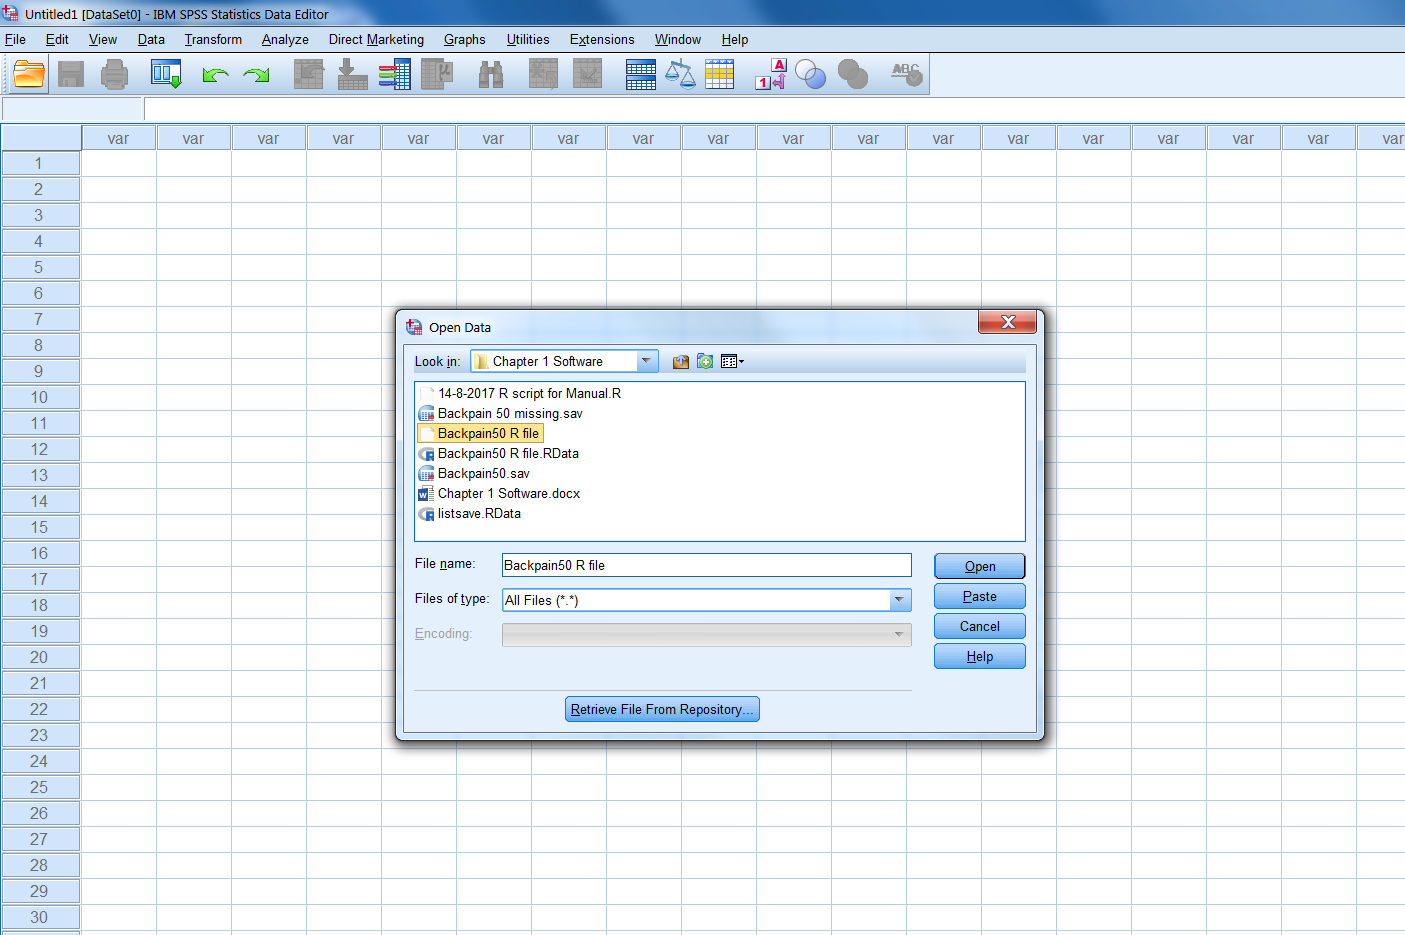
\includegraphics[width=0.95\linewidth]{images/fig1.18} 

}

\caption{Choosing the dataset to import in SPSS}\label{fig:fig18}
\end{figure}

Then click Open (wait a couple of seconds) and click on next. You will
see the following window that is part of the Text Import Wizard
procedure in SPSS (Figure \ref{fig:fig19}):

\begin{figure}

{\centering 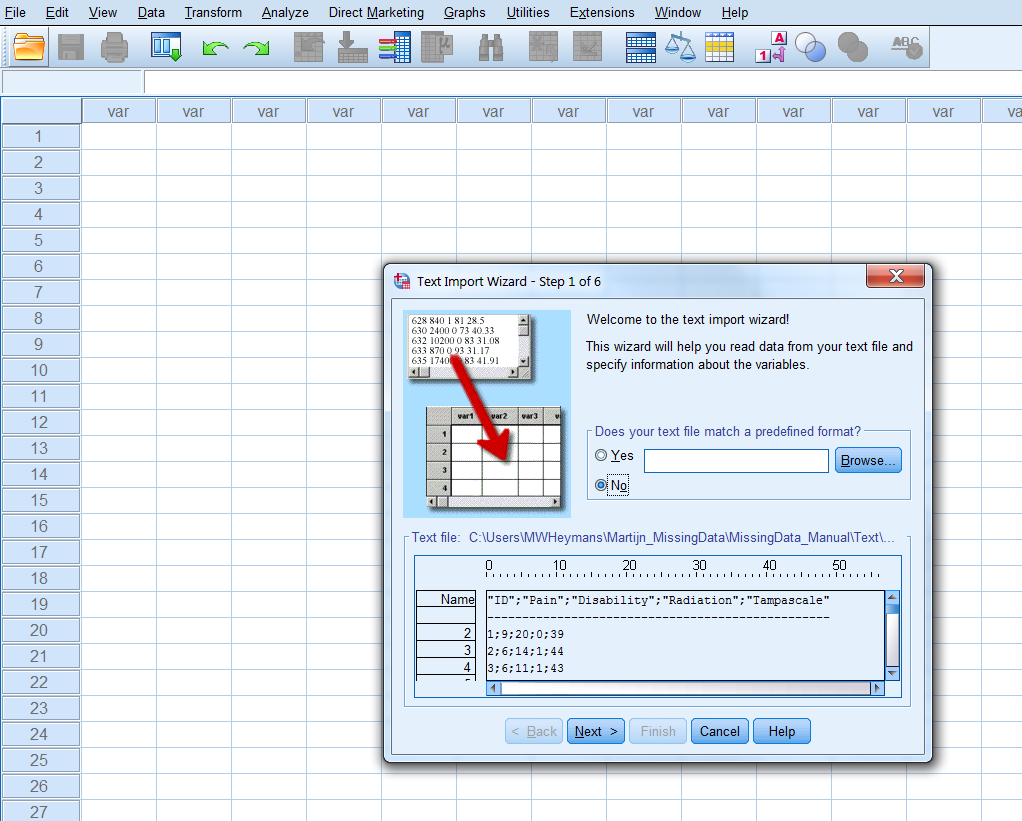
\includegraphics[width=0.95\linewidth]{images/fig1.19} 

}

\caption{Step 1 of the Text Import Wizard}\label{fig:fig19}
\end{figure}

Then click the ``Next \textgreater{}'' button 5 times, passing by the
following windows:

Step 2 of 6 (Figure \ref{fig:fig20}): To change how variables are
arranged: here delimited To include variable names included at the top
of the file: here Yes. To set the decimal symbol: here a comma.

\begin{figure}

{\centering 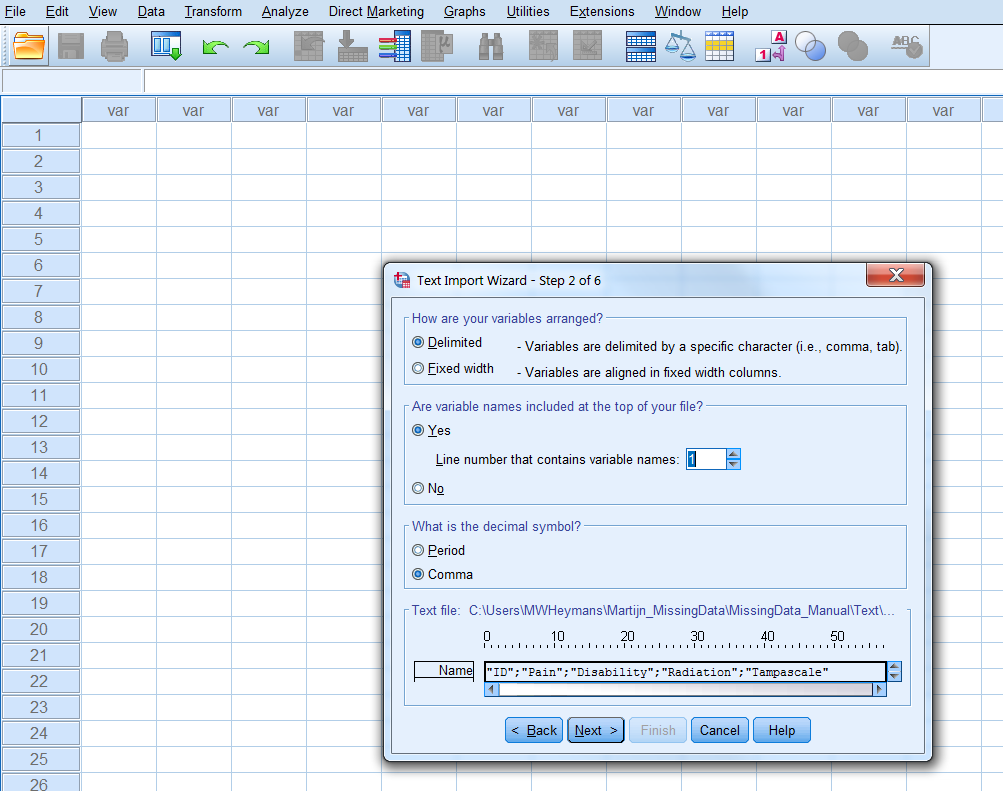
\includegraphics[width=0.95\linewidth]{images/fig1.20} 

}

\caption{Step 2 of the Text Import Wizard}\label{fig:fig20}
\end{figure}

Step 3 of 6 (Figure \ref{fig:fig21}):

On which line number begins the first case: here 2 How cases are
represented: Each line is a case. How many cases you want to import:
here all cases.

\begin{figure}

{\centering 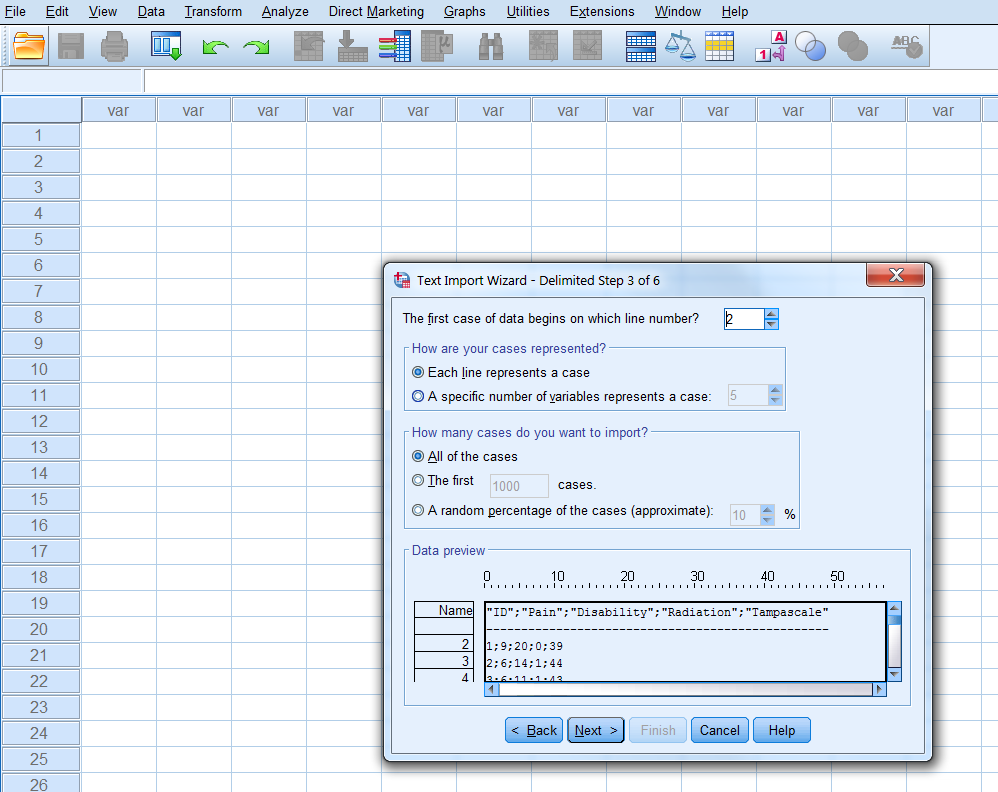
\includegraphics[width=0.95\linewidth]{images/fig1.21} 

}

\caption{Step 3 of the Text Import Wizard}\label{fig:fig21}
\end{figure}

Step 4 of 6 (Figure \ref{fig:fig22}): The delimiters that appear between
variables; here the Semicolon. The text qualifier: here Double quote.
Remove trailing spaces from string values: skip.

\begin{figure}

{\centering 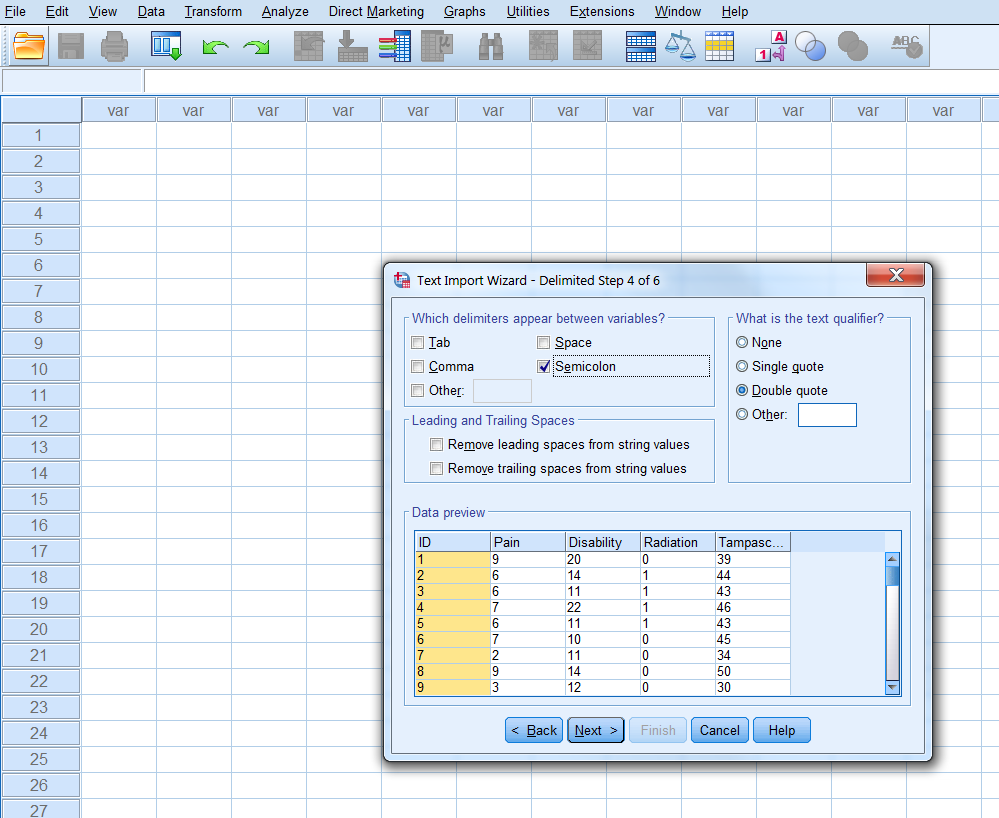
\includegraphics[width=0.95\linewidth]{images/fig1.22} 

}

\caption{Step 4 of the Text Import Wizard}\label{fig:fig22}
\end{figure}

Step 5 of 6 (Figure \ref{fig:fig23}): Here you overwrite the Data format
of the variable (you can also change that in the Variable View window,
when the data has been read in).

\begin{figure}

{\centering 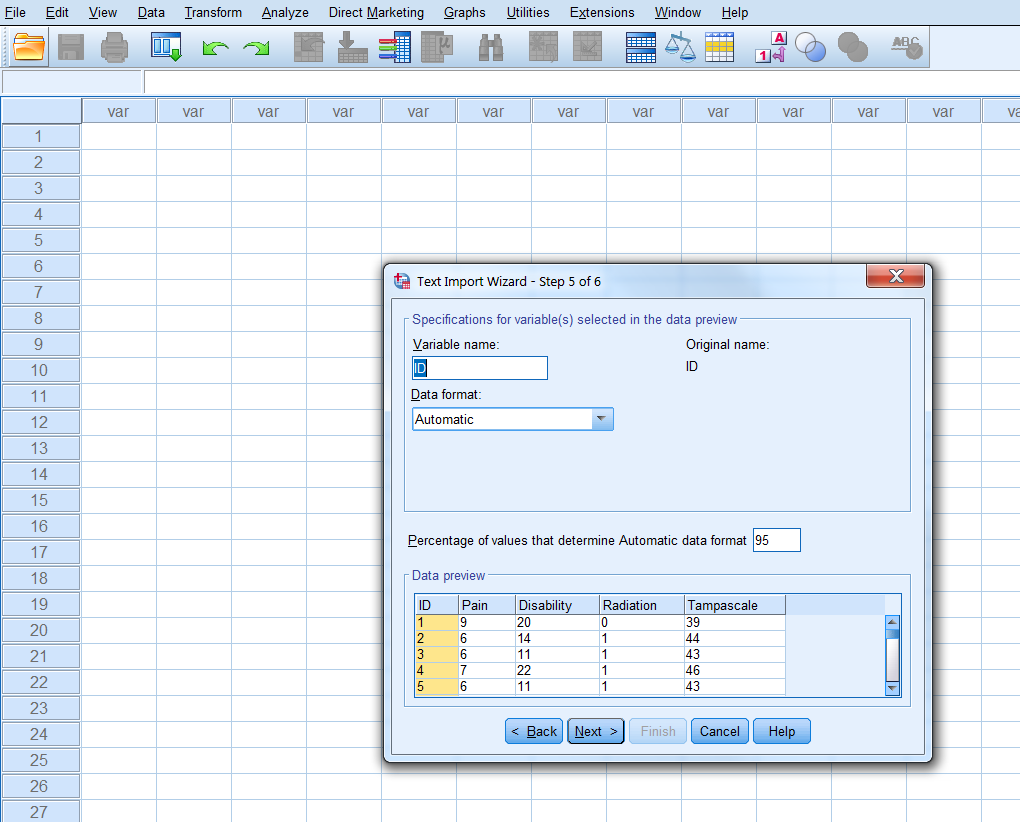
\includegraphics[width=0.95\linewidth]{images/fig1.23} 

}

\caption{Step 5 of the Text Import Wizard}\label{fig:fig23}
\end{figure}

Step 6 of 6: To save your specifications of the previous steps into a
separate file (Figure \ref{fig:fig24}).

\begin{figure}

{\centering 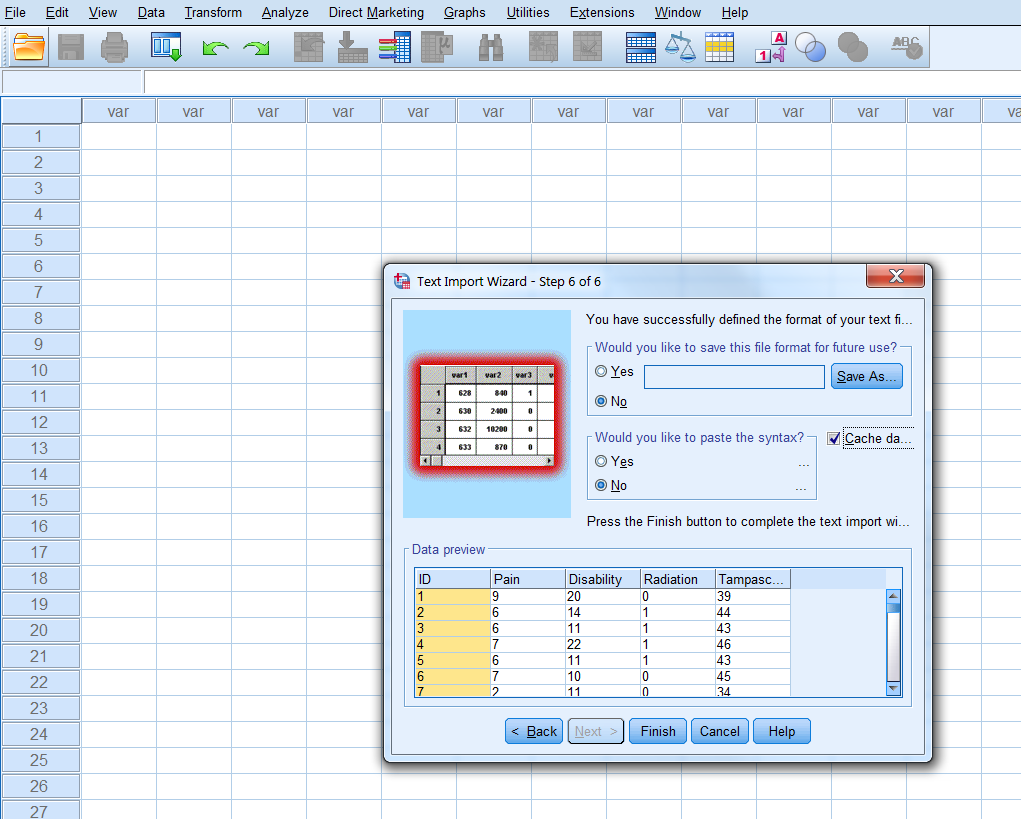
\includegraphics[width=0.95\linewidth]{images/fig1.24} 

}

\caption{Step 6 of the Text Import Wizard}\label{fig:fig24}
\end{figure}

Then click finish and the is imported in a new SPSS file. In that file
you can of course change all kind of variable and data settings in the
Variable View Window.

You can also skip step 2 to 5 by clicking the Finish button twice when
you are at step 1. Than you use all default settings, which is most of
the times a good option.

\subsection{Installing R Packages}\label{installing-r-packages}

When R is installed on your computer also a folder called library is
created. This folder contains packages that are part of the basic
installation. A package is a collection of different functions written
in the R language. Besides packages that are part of the basic
installation of R there are also packages that are not part of the basic
installation but are written by others, i.e.~the add-on packages.
Packages can be downloaded from the CRAN website
(\url{https://cran.r-project.org/}). Currently, there are thousands of
user-written packages available on the CRAN website.

Before you can use a specific package that is not part of the basic
installation, you have to install it in your R library. In this manual
we will use the mice package to do all kind of imputation procedures,
such as multiple imputation. mice is not part of the R basic
installation and you have to install it first. There are several
procedures in RStudio to install a package. One way is to use the
install.packages function in the Console window:

\begin{Shaded}
\begin{Highlighting}[]
\KeywordTok{install.packages}\NormalTok{(}\StringTok{"mice"}\NormalTok{)}
\end{Highlighting}
\end{Shaded}

The mice package will be automatically downloaded from the CRAN website.

Another way is to use the window on the right site below and go to the
Packages tab. When you click ``Install'' a new window is opened. Than
you can type ``mice'' on the blank line under ``Packages (separate
multiple with space or comma):'' (Figure \ref{fig:fig25} and Figure
\ref{fig:fig26}).

\begin{figure}

{\centering 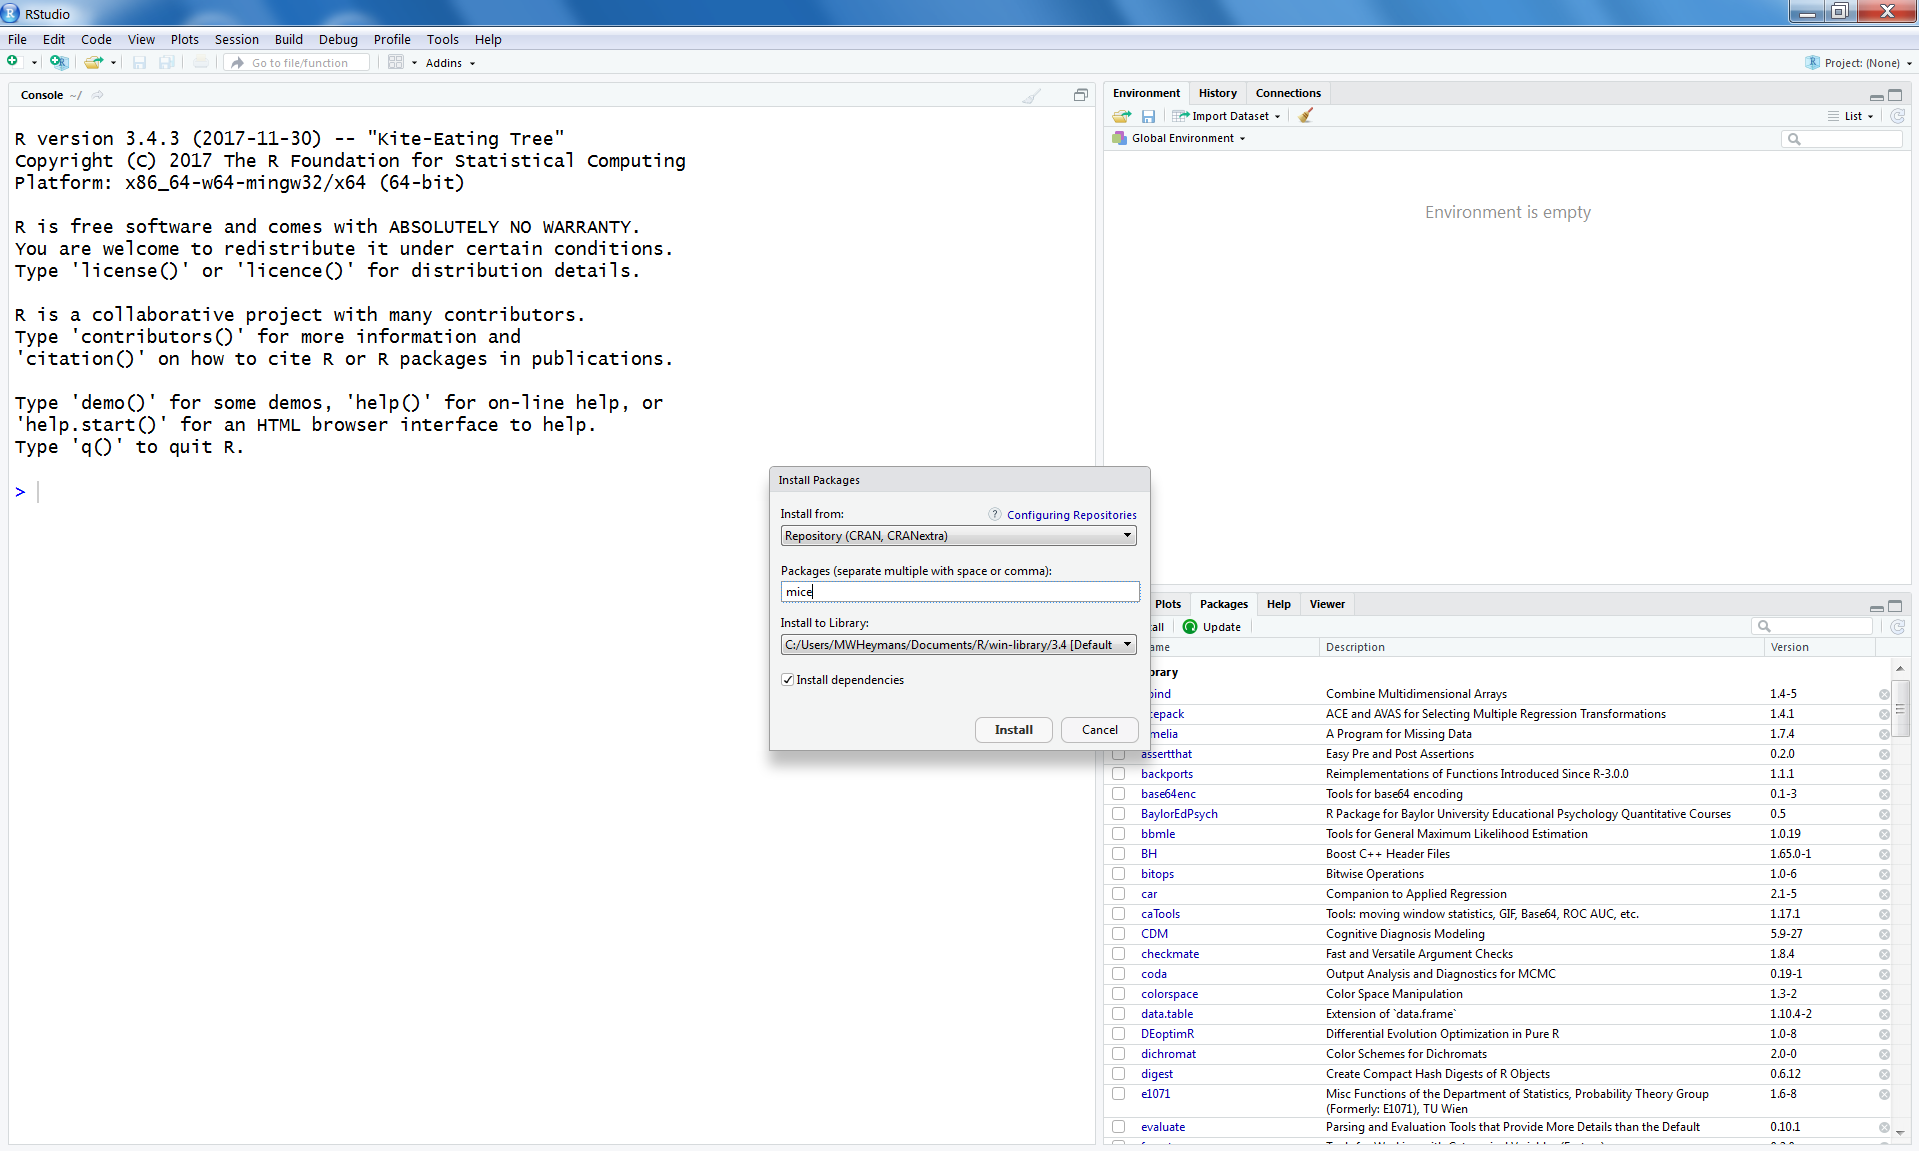
\includegraphics[width=0.95\linewidth]{images/fig1.25a} 

}

\caption{Install packages Window in RStudio to install packages from the CRAN website}\label{fig:fig25}
\end{figure}

\begin{figure}

{\centering 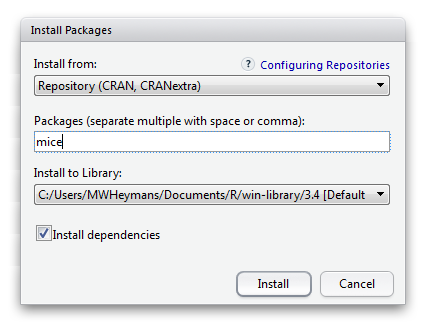
\includegraphics[width=0.95\linewidth]{images/fig1.25b} 

}

\caption{Enlarged Install packages Window in RStudio to install packages from the CRAN website}\label{fig:fig26}
\end{figure}

After you have clicked on ``Install'' the package will be downloaded
from the CRAN website automatically and will be listed in the Package
list named ``User Library''.

Another way is to go to the CRAN website and download the package as a
zip file in a directory on your computer, for example your working
directory or in your library. Again use the window on the right site
below and go to the Packages tab. When you choose Install a new window
is opened. Now under ``Install from:'' choose for ``Package Archive File
(.zip; .tar.gz)'' (Figure \ref{fig:fig27} and Figure \ref{fig:fig28}).
Than you can browse to the zip file and install the package.

\begin{figure}

{\centering 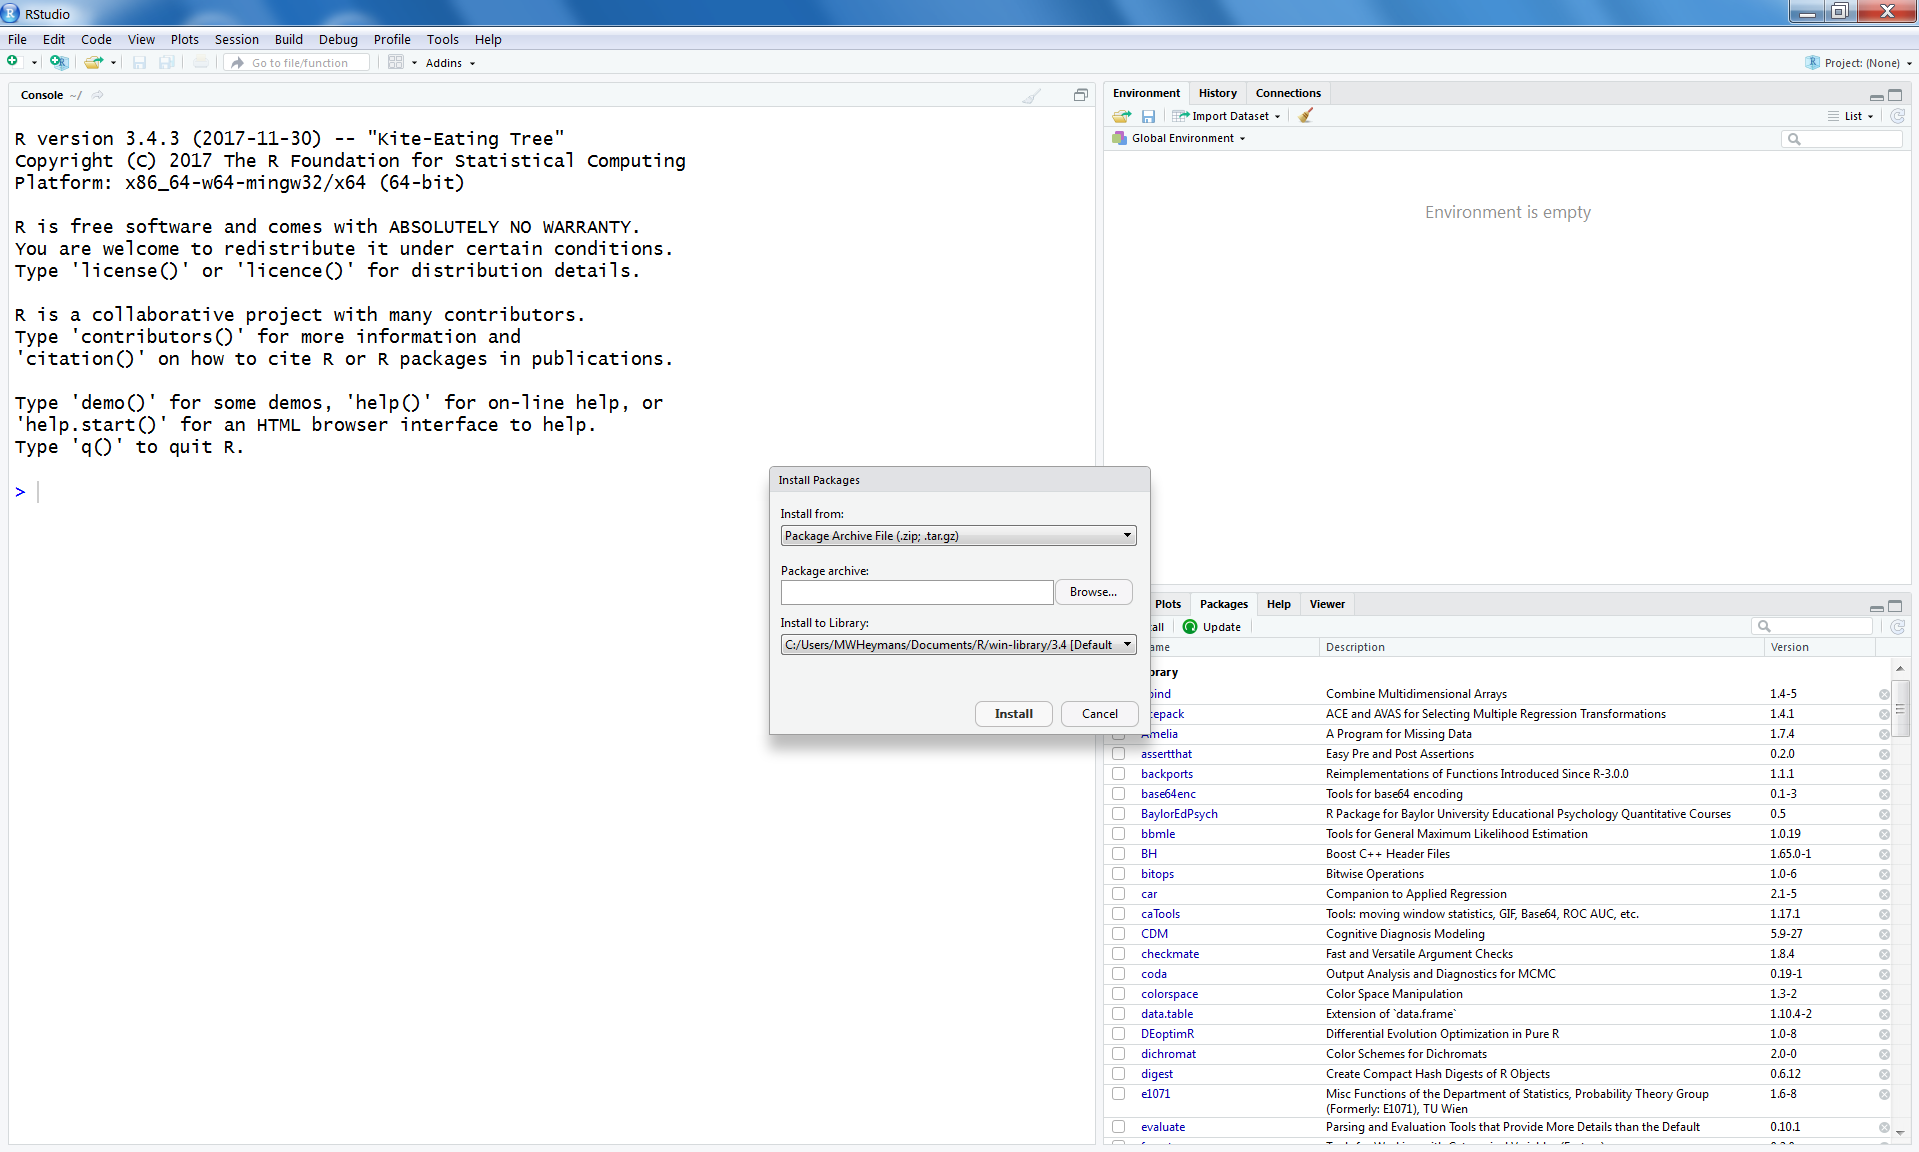
\includegraphics[width=0.95\linewidth]{images/fig1.26a} 

}

\caption{Install packages Window in RStudio to install packages from zip files}\label{fig:fig27}
\end{figure}

\begin{figure}

{\centering 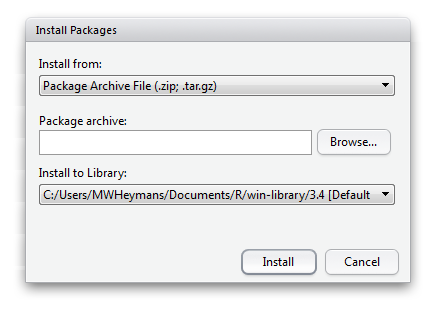
\includegraphics[width=0.95\linewidth]{images/fig1.26b} 

}

\caption{Enlarged Install packages Window in RStudio to install packages from zip files}\label{fig:fig28}
\end{figure}

\subsection{Loading R Packages}\label{loading-r-packages}

Once an add-on (user written) R package has been installed you have to
load it to get access to all functions that are part of that package. To
load a library, you can use the function library() or require().

You have to load add-on packages each time you start a new R session.

\subsection{Updating R Packages}\label{updating-r-packages}

To keep the add-on packages up to date you can use the update.packages()
function.

\begin{Shaded}
\begin{Highlighting}[]
\KeywordTok{update.packages}\NormalTok{()}
\end{Highlighting}
\end{Shaded}

R will ask you if you want to update each package. If you type ``y'' in
the Console window, R will update the package.

In RStudio updating packages can be done in the Package tab as well. You
can click on the Update button. A new window will open that contains a
list of all packages that need to be updated. Subsequently you can
select the packages you want to update.

\subsection{Useful Missing data Packages and
links}\label{useful-missing-data-packages-and-links}

The main package that we will use in this manual is mice which stand for
Multivariate Imputation by Chained Equations (MICE) (Van Buuren, 2009).
Other packages that can be used to impute data or that can be used to do
analyses after imputation are listed below.

\textbf{miceadds} Package contains some additional multiple imputation
functions (Robitzsch et al., 2017).
\href{https://cran.r-project.org/web/packages/miceadds/index.html}{See
for more information.}

\textbf{micemd} Package contains additional functions for the mice
package to perform multiple imputation in two-level (Multilevel) data
(Audigier \& Resche-Rigon, 2017).
\href{https://cran.r-project.org/web/packages/micemd/index.html}{See for
more information.}

\textbf{mi} Provides functions for data manipulation, imputing missing
values in an approximate Bayesian framework, diagnostics of the models
used to generate the imputations, confidence-building mechanisms to
validate some of the assumptions of the imputation algorithm, and
functions to analyze multiply imputed data sets (Gelman et al., 2015).
\href{https://cran.r-project.org/web/packages/mi/index.html}{See for
more information.}

\textbf{MItools} Small package to perform analyses and combine results
from multiple-imputation datasets (Lumley, 2015).
\href{https://cran.r-project.org/web/packages/mitools/index.html}{See
for more information.}

\textbf{norm} Package is for the Analysis of multivariate normal
datasets with missing values. It contains the mi.inference function.
This function combines estimates and standard errors to produce a single
inference. Uses the technique described by Rubin (1987), which are
called the Rubin's Rules (RR) (Novo, 2015).
\href{https://cran.r-project.org/web/packages/norm/index.html}{See for
more information.}

\textbf{vim (visualization and imputation of missing values)} Package
includes tools for the visualization of missing and/or imputed values.
In addition, the quality of imputation can be visually explored using
various univariate, bivariate, multiple and multivariate plot methods
(Templ et al., 2017).
\href{https://cran.r-project.org/web/packages/mi/index.html}{See for
more information.}

\textbf{BaylorEdPsych} Package for Baylor University Educational
Psychology Quantitative Courses. This package included Little's MCAR
test (Beaujean, 2015).
\href{https://cran.r-project.org/web/packages/BaylorEdPsych/index.html}{See
for more information.}

\textbf{MKmisc} Contains several functions for statistical data
analysis; e.g.~for sample size and power calculations, computation of
confidence intervals, and generation of similarity matrices. This
package contains the mi.t.test function for pooling t-tests after
multiple imputation (Kohl, 2016).
\href{https://cran.r-project.org/web/packages/MKmisc/index.html}{See for
more information.}

\textbf{mvnmle} Package estimates the maximum likelihood estimate of the
mean vector and variance-covariance matrix for multivariate normal data
with missing values. This package is needed for the mlest function this
is used for Little's MCAR test in Cahpter 2.
\href{https://cran.r-project.org/web/packages/mvnmle/index.html}{See for
more information.}

\part{Part II: Basic Missing Data
Handling}\label{part-part-ii-basic-missing-data-handling}

\chapter{Missing Data Evaluation}\label{missing-data-evaluation}

Before you decide what to do with your missing data it is important to
consider the reasons and probable causes of your missing data problem.
With that information you can compose an analysis plan to deal with the
missing data in your dataset. In this Chapter, you will learn how to
explore and evaluate missing data in SPSS and R and why it is important
to think about the reasons for missing data. Knowledge about this helps
you to solve the missing data problem.

\section{Definition of Missing Data}\label{definition-of-missing-data}

\subsection{Defining Missing Data in
SPSS}\label{defining-missing-data-in-spss}

Missing data in SPSS can be defined in two ways, as a system missing or
user missing value. System missing data are missing data that is not
present in the dataset and can be recognized by an empty cell (or dot).
User missing data are data that are coded as missing values in the
dataset by the user for some specific kind of reason. As an example we
use a small dataset with 50 Backpain patients consisting of male (coded
as 1) and female (coded as 0) patients (Figure \ref{fig:fig2-1}). For
the female patients in this dataset the duration of a previous pregnancy
was regisered in the Gestational Age (GA) variable.

\begin{figure}

{\centering 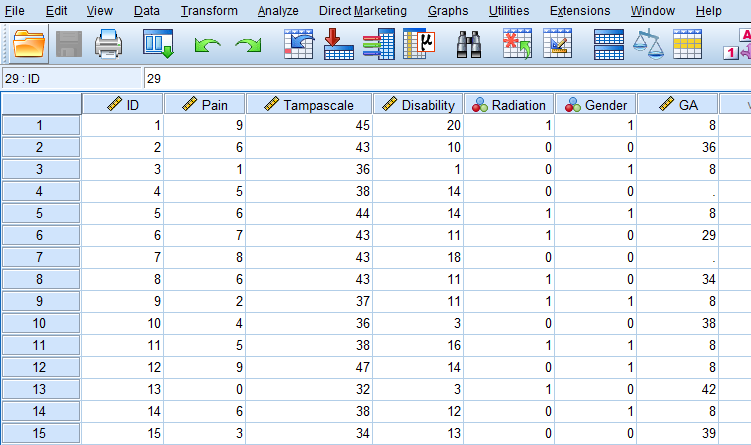
\includegraphics[width=0.9\linewidth]{images/fig2.1} 

}

\caption{SPSS dataset containing variables with system and user missing data}\label{fig:fig2-1}
\end{figure}

The Variable GA in the dataset consists of different values: pregenancy
durations in weeks, such as 36 and 29, but also the value 8 and empty
cells. The value 8 is specified by the user to exclude males from
further analysis that include the GA variable. This is a user missing
value, that was indicated because males cannot be pregnant. The system
missing values are recognizable by the empty cells (or dots) in the
dataset, and these indicate the missing GA values for women who did not
report the GA for their pregnancy. It makes no difference if we code the
missing values as a system or user missing value in SPSS, because both
kinds of missing values are recognized as missing values by SPSS and
will be excluded from further analyses.

\subsection{Defining Missing data in
R}\label{defining-missing-data-in-r}

In R the missing values are denoted by \texttt{NA} which means ``Not
Available''. If we open the same dataset as above in R we get the
following result.

\begin{Shaded}
\begin{Highlighting}[]
\KeywordTok{library}\NormalTok{(haven)}
\NormalTok{dataset <-}\StringTok{ }\KeywordTok{read_sav}\NormalTok{(}\StringTok{"data/CH2 example.sav"}\NormalTok{)}
\KeywordTok{head}\NormalTok{(dataset,}\DecValTok{10}\NormalTok{) }\CommentTok{# Data of first 10 patients is shown}
\end{Highlighting}
\end{Shaded}

\begin{verbatim}
## # A tibble: 10 x 7
##       ID  Pain Tampascale Disability Radiation Gender    GA
##    <dbl> <dbl>      <dbl>      <dbl>     <dbl>  <dbl> <dbl>
##  1     1     9         45         20         1      1     8
##  2     2     6         43         10         0      0    36
##  3     3     1         36          1         0      1     8
##  4     4     5         38         14         0      0    NA
##  5     5     6         44         14         1      1     8
##  6     6     7         43         11         1      0    29
##  7     7     8         43         18         0      0    NA
##  8     8     6         43         11         1      0    34
##  9     9     2         37         11         1      1     8
## 10    10     4         36          3         0      0    38
\end{verbatim}

The Variable Gestational Age (GA) contains the values for GA (e.g.~36,
29, etc.), the value 8 for males and the NA's. In R the value 8 will be
treated as a real value, so we have to recode that value to \texttt{NA}
by using the following code to convert an 8 into an \texttt{NA} for the
males.

\begin{Shaded}
\begin{Highlighting}[]
\NormalTok{dataset}\OperatorTok{$}\NormalTok{GA[dataset}\OperatorTok{$}\NormalTok{GA}\OperatorTok{==}\DecValTok{8}\NormalTok{] <-}\StringTok{ }\OtherTok{NA}
\KeywordTok{head}\NormalTok{(dataset,}\DecValTok{10}\NormalTok{)}
\end{Highlighting}
\end{Shaded}

\begin{verbatim}
## # A tibble: 10 x 7
##       ID  Pain Tampascale Disability Radiation Gender    GA
##    <dbl> <dbl>      <dbl>      <dbl>     <dbl>  <dbl> <dbl>
##  1     1     9         45         20         1      1    NA
##  2     2     6         43         10         0      0    36
##  3     3     1         36          1         0      1    NA
##  4     4     5         38         14         0      0    NA
##  5     5     6         44         14         1      1    NA
##  6     6     7         43         11         1      0    29
##  7     7     8         43         18         0      0    NA
##  8     8     6         43         11         1      0    34
##  9     9     2         37         11         1      1    NA
## 10    10     4         36          3         0      0    38
\end{verbatim}

The \texttt{NA} values will be recognized as missing values.

Within most functions in R the handling of \texttt{NA} values has to be
defined, otherwise the function returns an NA as a result. For example,
the following code to obtain the mean of Gestational Age results in an
\texttt{NA} because the handling of missing data is not defined within
the function.

\begin{Shaded}
\begin{Highlighting}[]
\KeywordTok{mean}\NormalTok{(dataset}\OperatorTok{$}\NormalTok{GA)}
\end{Highlighting}
\end{Shaded}

\begin{verbatim}
## [1] NA
\end{verbatim}

To obtain the mean of the observed data the statement
\texttt{na.rm\ =\ TRUE} can be added.

\begin{Shaded}
\begin{Highlighting}[]
\KeywordTok{mean}\NormalTok{(dataset}\OperatorTok{$}\NormalTok{GA, }\DataTypeTok{na.rm =} \OtherTok{TRUE}\NormalTok{)}
\end{Highlighting}
\end{Shaded}

\begin{verbatim}
## [1] 35.09524
\end{verbatim}

The \texttt{na.rm\ =\ TRUE} statement in the mean-function, indicates
that values that are \texttt{NA} need to be removed before the analysis
is executed. Another \texttt{NA} handling procedure that is regularly
used in functions is called \texttt{na.action} with as options
\texttt{na.fail}, \texttt{na.omit}, \texttt{NULL} (no action) and
\texttt{na.exclude}. For more information about na.action options you
can look at the help-file by typing \texttt{?na.action} in the Console
window.

\section{Missing data Patterns}\label{missing-data-patterns}

To get an idea about the complexity of the missing data problem in your
dataset and information about the location of the missing values, the
missing data pattern can be evaluated. Historically, the missing data
pattern was an important starting point to choose the missing data
handling method (\citet{little1987statistical}). Currently, the missing
data pattern is less important because the most advanced missing data
analysis method as multiple imputation can handle almost any missing
data pattern. We will discuss some frequently seen missing data
patterns, which are graphically displayed in Figure \ref{fig:fig2-2}.

\begin{figure}

{\centering 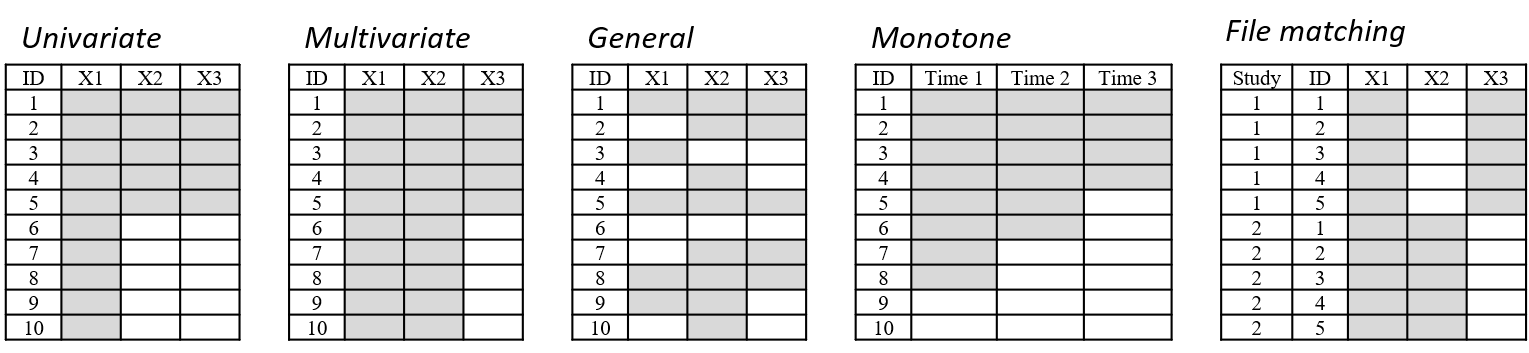
\includegraphics[width=0.9\linewidth]{images/fig2.2} 

}

\caption{Missing data patterns (ID means person identification number, X1 to X3 represent variables, Time 1 to 3 means that data is measured at 3 time points over time, Study means study number). The white cells represent the missing data}\label{fig:fig2-2}
\end{figure}

A univariate missing data pattern is a pattern with missing values in
only one variable. An example of such a pattern is when the independent
variables are completely observed, but the outcome variable is not, or
when a selection of subjects refuse to fill in a specific question such
as their income level. The second and third pattern are examples of
multivariate missing data patterns, where multiple variables contain
missing values. The second pattern is an example where subjects miss
values of the same two variables and the third pattern a more general
pattern where different subject miss different variable scores. A
monotone pattern of missing data may occur in a longitudinal study with
data repeatedly assessed over time, and subjects ``drop-out'' of the
study (fourth pattern). For example in a study on elderly where persons
get too frail to participate as they get older or just because persons
do not want to attend the study anymore because they loose interest and
don't feel like filling in questionnaires. A pattern called ``file
matching''" can be observed when data from several studies is merged for
an individual participant data analysis and some variables are not
assessed in all studies. In this example, one variable is observed in
both studies (X1), but X2 and is only observed in study 1 and X3 only in
study 2.

\subsection{Exploring Missing data patterns in
SPSS}\label{exploring-missing-data-patterns-in-spss}

To evaluate the missing data pattern, we use the options of the Missing
Value Analysis (MVA) procedure in SPSS (\citet{spss75}). The example
dataset contains information on 9 study variables for 150 back pain
patients. The continuous variables are Pain, Tampa scale, Disability,
Body weight, Body length and Age. The dichotomous variables are
Radiation in the leg, Smoking, and Gender. Only the variables Gender and
Age are completely observed.

To access the MVA function in the SPSS menu choose:

\begin{quote}
Analyze -\textgreater{} Missing Value Analysis\ldots{}
\end{quote}

A new window will open that is called ``Missing Value Analysis''.

In this menu, transfer all continuous variables to the Quantitative
variables window and the categorical variables to the Categorical
variables window. Then select the Patterns option. From the Patterns
menu (Figure \ref{fig:fig2-4} select the options
\texttt{Tabulated\ cases,\ grouped\ by\ missing\ value\ patterns} and
\texttt{sort\ variables\ by\ missing\ value\ pattern}. To obtain the
full list of all patterns that occur in the data, set the ``Omit
patterns with less than 1\% of cases'' at 0\%, then click continue and
OK.

\begin{figure}

{\centering 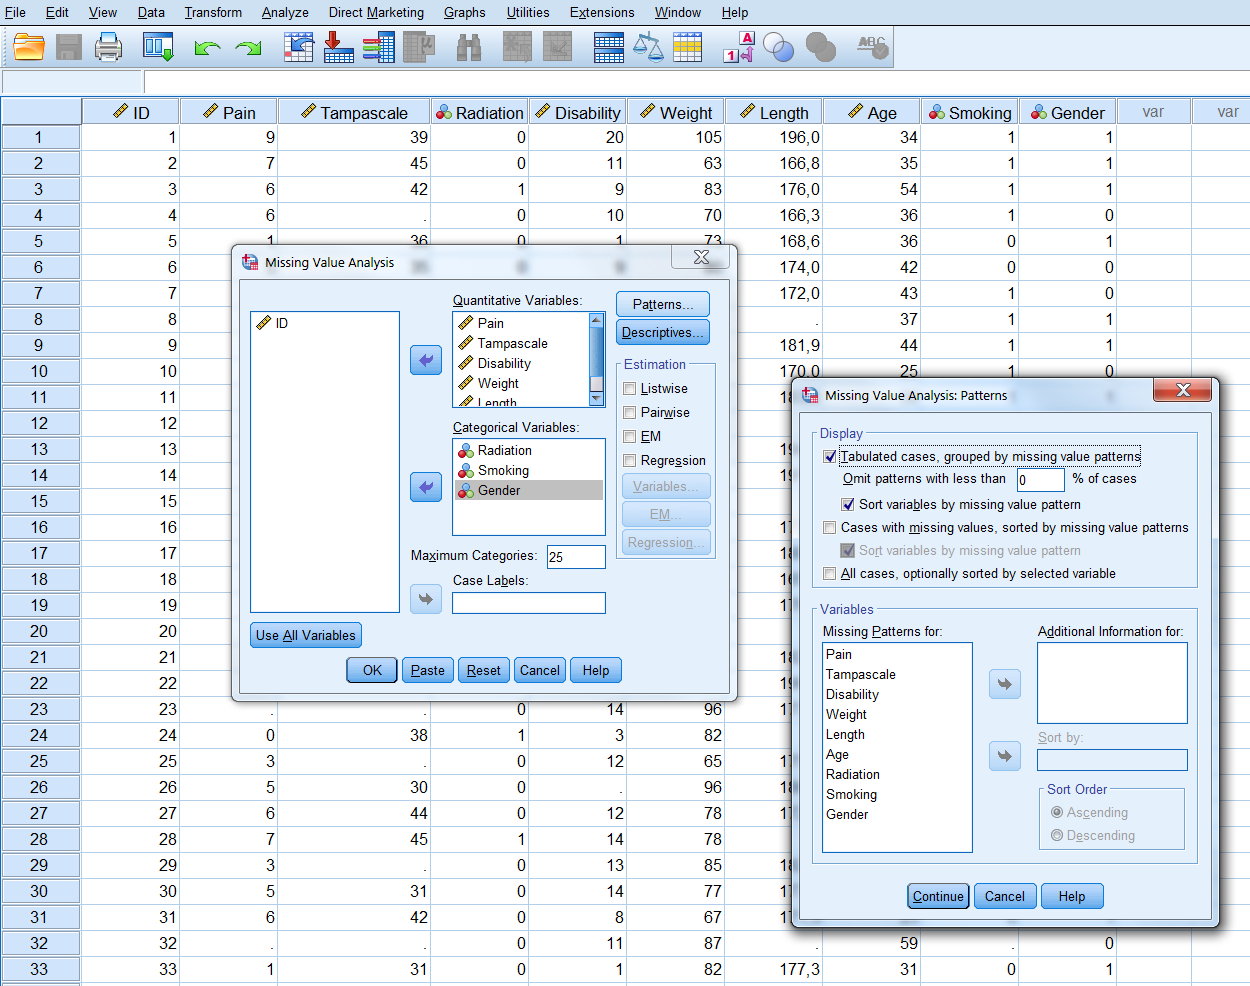
\includegraphics[width=0.9\linewidth]{images/fig2.4} 

}

\caption{The Patterns menu}\label{fig:fig2-4}
\end{figure}

By default, univariate statistics are presented that include output
information about the number and percentages of missing data and
descriptive statistics for each variable (Figure \ref{fig:tab2-1}).

Information about the missing data patterns is provided in the Tabulated
patterns table. On the left column of that table, named ``Number of
Cases'', the number of cases are presented with that specific missing
data pattern. In our example, there are 75 cases without any missing
value and 13 cases with a missing value in only the Tampa scale variable
(see row 1 and 2 in (Figure \ref{fig:tab2-1}). In the right column of
that table named ``Complete if\ldots{}'', the total number of subjects
is presented if the variables that contain missing data in that pattern
are not used in the analysis. Those variables are marked with the ``X''
symbol. For example, 88 subjects remain in the analysis when the
variable tampa scale is not used in the analysis, these are the 75
subjects that have completely observed data on top of the 13 subjects
with missing data in the Tampa scale variable only.

\begin{figure}

{\centering 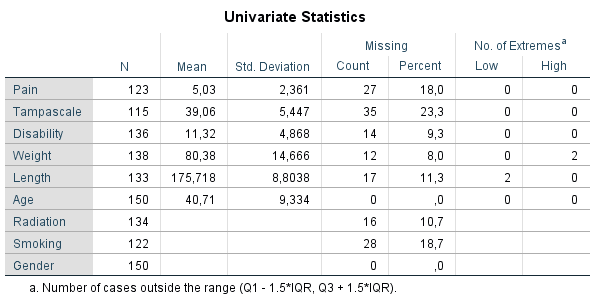
\includegraphics[width=0.9\linewidth]{images/tab2.1a} 

}

\caption{Descriptive missing data statistics and the missing data patterns.}\label{fig:tab2-1}
\end{figure}\begin{figure}

{\centering 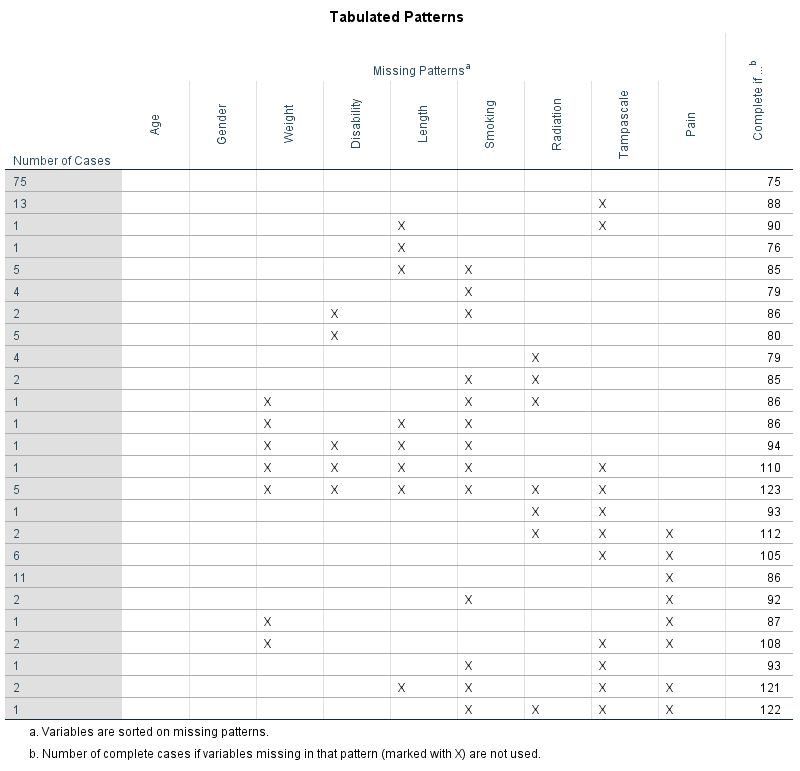
\includegraphics[width=0.9\linewidth]{images/tab2.1b} 

}

\caption{Descriptive missing data statistics and the missing data patterns.}\label{fig:tab2-1}
\end{figure}

Another way to obtain information about the missing data patterns is by
accessing the Multiple Imputation menu option. To access this menu,
choose:

\begin{quote}
Analyze -\textgreater{} Multiple Imputation -\textgreater{} Analyze
Patterns\ldots{}
\end{quote}

\begin{figure}

{\centering 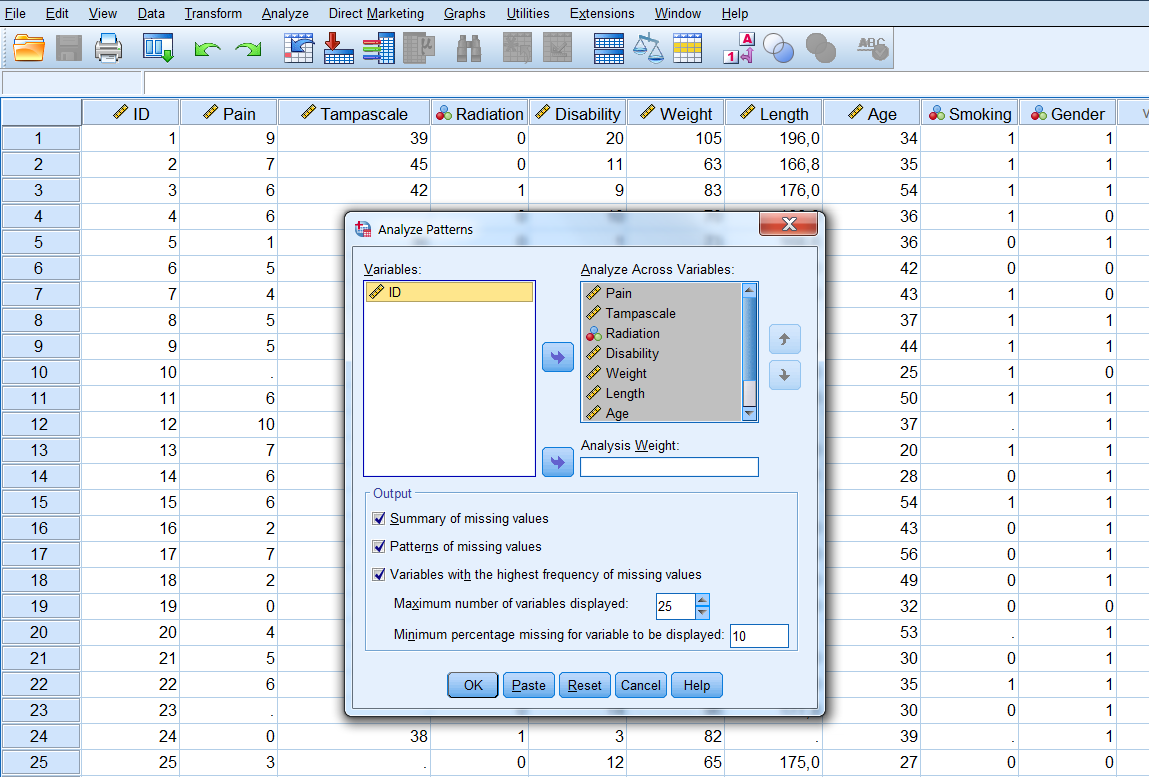
\includegraphics[width=0.9\linewidth]{images/fig2.5} 

}

\caption{Analyse Patterns menu.}\label{fig:fig2-5}
\end{figure}

Now transfer all variables for the missing value analysis to the window
``Analyze Across Variables''. The following output options can be
selected:

\begin{itemize}
\tightlist
\item
  Summary of missing values: displays missing data information in pie
  charts, Patterns of missing values (displays tabulated patterns of
  missing values.
\item
  Variables with the highest frequency of missing values: displays a
  table of analysis variables sorted by percent of missing values in
  decreasing order. .
\item
  Minimum percentage missing for varaibles to be displayed: set at 0 to
  obtain the full list of all patterns.
\item
  Adjust the maximum number of variables displayed.
\end{itemize}

The following output will be displayed after selecting all options:

\begin{figure}

{\centering 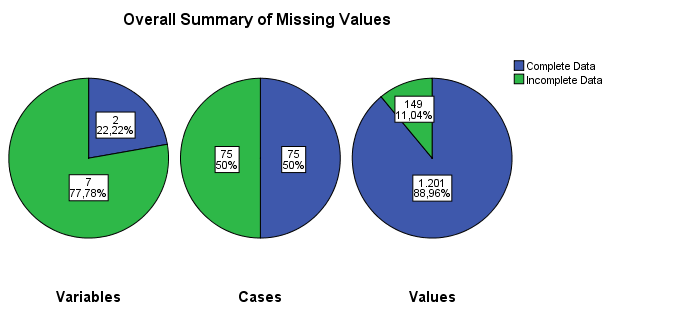
\includegraphics[width=0.9\linewidth]{images/fig2.6a} 

}

\caption{Output as a result of the Analyze Patterns menu under Multiple Imputation.}\label{fig:fig2-6}
\end{figure}\begin{figure}

{\centering 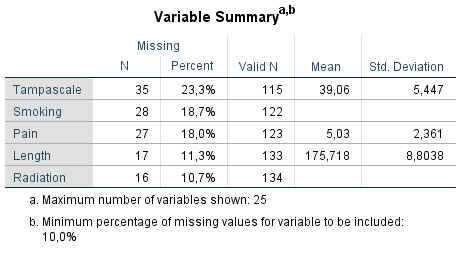
\includegraphics[width=0.9\linewidth]{images/fig2.6b} 

}

\caption{Output as a result of the Analyze Patterns menu under Multiple Imputation.}\label{fig:fig2-6}
\end{figure}\begin{figure}

{\centering 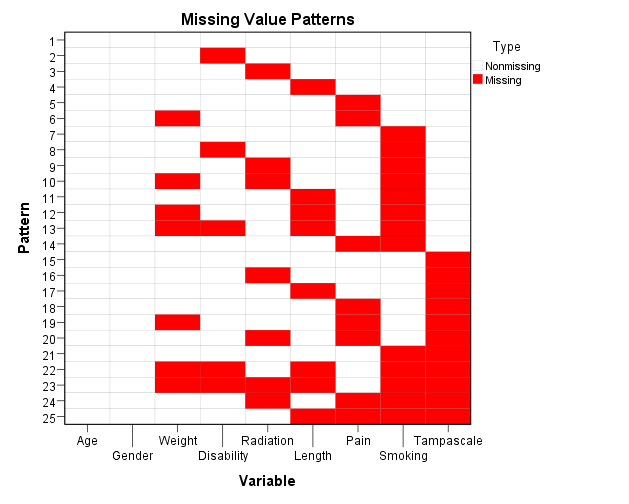
\includegraphics[width=0.9\linewidth]{images/fig2.6c} 

}

\caption{Output as a result of the Analyze Patterns menu under Multiple Imputation.}\label{fig:fig2-6}
\end{figure}\begin{figure}

{\centering 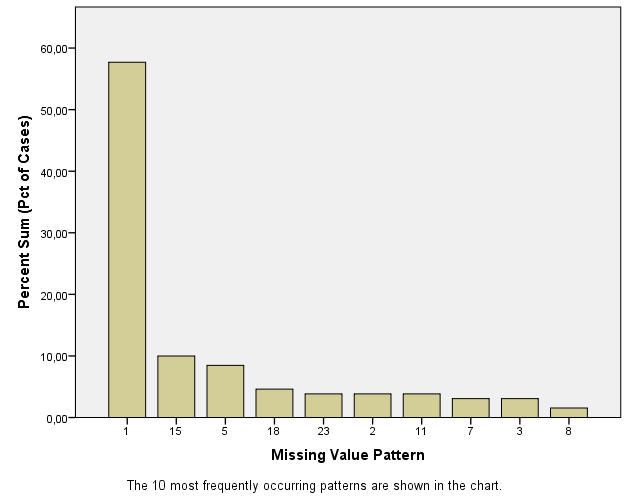
\includegraphics[width=0.9\linewidth]{images/fig2.6d} 

}

\caption{Output as a result of the Analyze Patterns menu under Multiple Imputation.}\label{fig:fig2-6}
\end{figure}

\subsection{Exploring Missing data patterns in
R}\label{exploring-missing-data-patterns-in-r}

To display the missing data patterns in R we can use the \texttt{mice}
or \texttt{VIM} package. We start with the \texttt{mice} package. This
package contains the \texttt{md.pattern} function that produces the
missing data pattern.

\begin{Shaded}
\begin{Highlighting}[]
\KeywordTok{library}\NormalTok{(mice)}
\KeywordTok{md.pattern}\NormalTok{(dataset)}
\end{Highlighting}
\end{Shaded}

\includegraphics{Book_MI_files/figure-latex/unnamed-chunk-54-1.pdf}

\begin{verbatim}
##    ID Pain Tampascale Disability Radiation Gender GA   
## 21  1    1          1          1         1      1  1  0
## 29  1    1          1          1         1      1  0  1
##     0    0          0          0         0      0 29 29
\end{verbatim}

The first row contains the variable names. Each other row represents a
missing data pattern. The 1's in each row indicate that the variable is
complete and the 0's indicate that the variable in that pattern contains
missing values. The first column on the left (without a column name)
shows the number of cases with a specific pattern and the column on the
right shows the number of variables that is incomplete in that pattern.
The last row shows the total number of missing values for each variable.

To obtain a visual impression of the missing data patterns in R the
\texttt{VIM} package can be used. That package contains the function
\texttt{aggr} that produces the univariate proportion of missing data
together with two graphs.

\begin{Shaded}
\begin{Highlighting}[]
\KeywordTok{library}\NormalTok{(VIM)}
\KeywordTok{aggr}\NormalTok{(dataset, }\DataTypeTok{col=}\KeywordTok{c}\NormalTok{(}\StringTok{'white'}\NormalTok{,}\StringTok{'red'}\NormalTok{), }\DataTypeTok{numbers=}\OtherTok{TRUE}\NormalTok{, }\DataTypeTok{sortVars=}\OtherTok{TRUE}\NormalTok{, }\DataTypeTok{cex.axis=}\NormalTok{.}\DecValTok{7}\NormalTok{, }\DataTypeTok{gap=}\DecValTok{3}\NormalTok{, }\DataTypeTok{ylab=}\KeywordTok{c}\NormalTok{(}\StringTok{"Percentage of missing data"}\NormalTok{,}\StringTok{"Missing Data Pattern"}\NormalTok{))}
\end{Highlighting}
\end{Shaded}

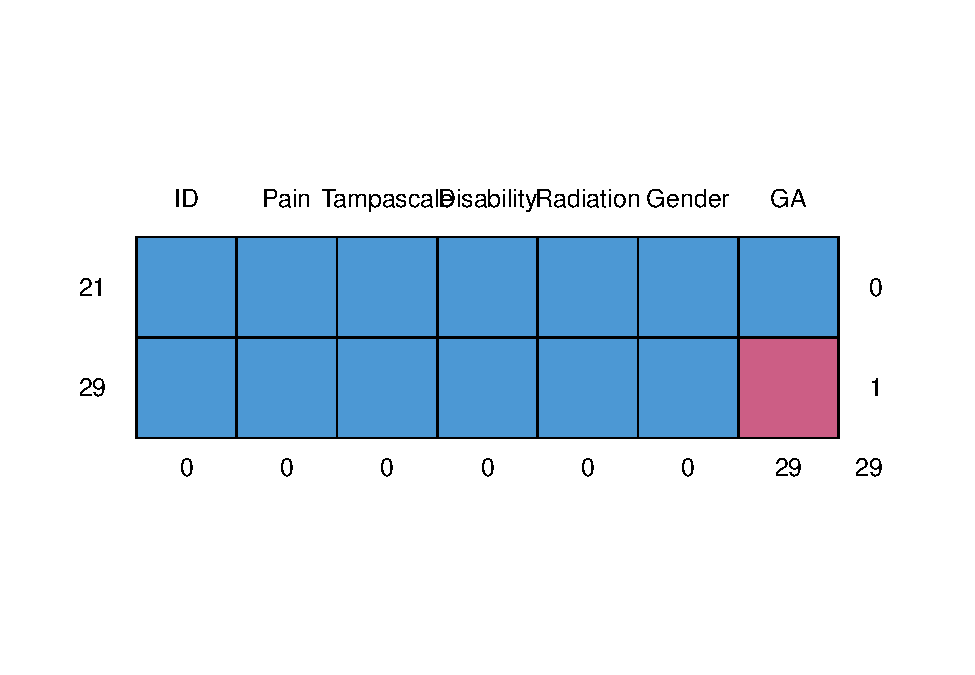
\includegraphics{Book_MI_files/figure-latex/unnamed-chunk-55-1.pdf}

\begin{verbatim}
## 
##  Variables sorted by number of missings: 
##    Variable Count
##          GA  0.58
##          ID  0.00
##        Pain  0.00
##  Tampascale  0.00
##  Disability  0.00
##   Radiation  0.00
##      Gender  0.00
\end{verbatim}

The variable names are shown at the bottom of the figures. The red cells
in the Missing data patterns figure indicate that those variables
contain missing values. We see that 0.500 or 50\% of the patterns do not
contain missing values in any of the variables. Of the total patterns,
8.67\% of the patterns have missing values in only the Tampa scale
variable.

\section{Missing data Mechanisms}\label{missing-data-mechanisms}

By evaluating the missing data patterns, we can get insight in the
location of the missing data. With respect to the missing data mechanism
we are interested in the underlying reasons for the missing values and
the relationships between variables with and without missing data. In
general, we can say that missing values are either random or non-random.
Random missing values may occur because subjects accidentally do not
answer some questions or that information of an entire subject is
accidentally not assessed. For example, a study subject has to fill out
some questionnaire instruments, gets distracted and misses a question
accidently or a questionnaire gets lost in the mail. Non-random missing
values may occur because subjects purposefully do not answer questions.
For example, subjects may be reluctant to answer questions about
sensitive topics like income, past crimes or sexual history. In 1976,
Donald Rubin introduced a typology for missing data that distincts
between random and non-random missing data situations, which are
abbreviated as MCAR, MAR and MNAR (\citet{Rubin1976}). These types of
missing data are still used as the basic missing data mechanisms. The
key idea behind Rubin's missing data mechanisms is that the probability
of missing data in a variable may or may not be related to the values of
other measured variables in the dataset. This means that we assume that
there is some kind of probability model for the missing data. With
probability we loosely mean the likelihood of a missing value to occur,
i.e.~if a variable has a lot of missing data, the probability of missing
data in that variable is high. This probability can be related to other
measured or not-measured variables. For example, when mostly older
people have missing values, the probability for missing data is related
to age. Moreover, the missing data mechanisms also assume a certain
relationship (or correlation) between observed variables and variables
with missing values in the dataset. The extend of the relation between
observed variables and the probability of missing data, distinguishes
the three missing data mechanisms. We will discuss the missing data
mechanisms in more detail below. As an example, we will use a study on
Low Back Pain (LBP). It is known that people with LBP may develop a fear
of movement (which is assessed by the Tampa scale) due to their pain in
the back. The idea is that these people believe that some underlying
serious problem causes their back pain and in order to prevent more
damage they are afraid to move their back and experience a high fear of
movement.

\subsection{Missing Completely At
Random}\label{missing-completely-at-random}

Data are Missing Completely At Random (MCAR) when the probability that a
value is missing, is unrelated to the value of other observed (or
unobserved) variables, and unrelated to values of the missing data
variable itself. An MCAR example in the LBP study could be that, LBP
patients had to come to a research center to fill in the Tampa scale
(fear of movement) questionnaire and other information for the study and
some of these patients were unable to leave their home, due to the flu.
In that case, there is no relationship between having the flu and the
scores on the Tampa scale or other study-related variables. This is
realistic because there is no evidence that patients with the flu, fear
their back problems more. For that reason, we can assume that the
missing data are MCAR. Another example is when respondents accidentally
skip questions in a questionnaire. Than the observed values of that
questionnaire are just a random sample of the entire dataset.

An MCAR missing data situation for the Tampa scale variable is
visualized in the MCAR column in Figure 2.7 below. Note that in real
live we do not know the completely observed data, but for educational
reasons, the completely observed Tampa scale variable is displayed as
well. When we compare the MCAR data to the complete Tampa scale variable
scores, we can observe that in the MCAR situation an equal number of
lower and higher values of the Tampa scale variable are missing (in
total 4 Tampa scores are missing, 2 for lower and 2 for higher values).
Also, the missing data in the Tampa scale do not seem to be related to
the values of another variable like pain; an equal number of Tampa scale
values is missing for patients with low pain scores as well as for
patients with higher pain scores. This means that the (observed)
probability of missing data in the Tampa scale variable will be equally
large for lower and higher values of the Tampa scale and of other
measured variables in the data (i.e.~Pain).

\begin{figure}

{\centering 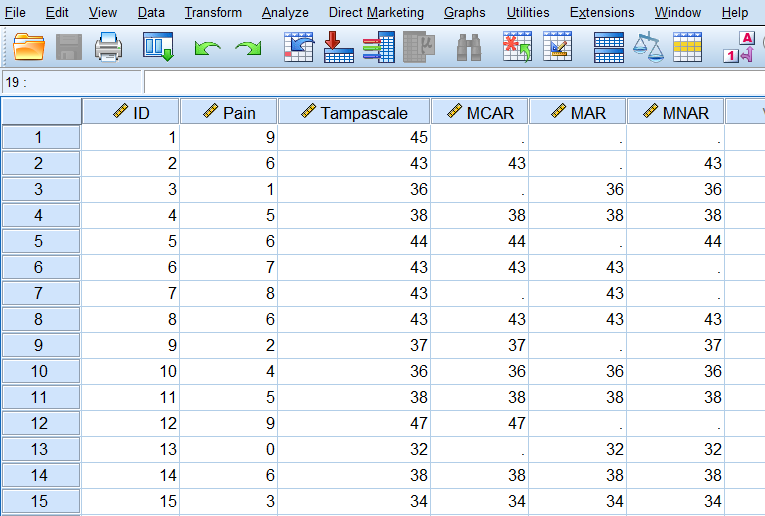
\includegraphics[width=0.9\linewidth]{images/fig2.7} 

}

\caption{Examples of MCAR, MAR and MNAR data.}\label{fig:fig2-7}
\end{figure}

\subsection{Missing At Random}\label{missing-at-random}

Data are Missing At Random (MAR) when the probability that a value for a
variable is missing is related to other observed values in the dataset
but not to the variable itself. An example of MAR data in the LBP study
is presented in the MAR column of Figure \ref{fig:fig2-7} and Figure
\ref{fig:tab2-3}. In Figure \ref{fig:fig2-7} you can see in the MAR
column that 4 Tampa scale scores are missing for pain scores that are ≥
6 and 1 for a pain score \textless{} 6, in other words the probability
of missing data in the Tampa scale scores is higher for patients with
higher pain scores. However, within the category of pain scores with
values ≥ 6, the Tampa scale scores are MCAR, because within each
category Tampa scale scores are randomly missing for lower and higher
values. As a consequence, means and standard deviations do not differ
between the observed and missing data for the Tampa scale variable. An
explanation for this phenomenon can be that patients with higher Tampa
scale scores were less likely to show up at a next Tampa scale
measurement because their back hurted more.

In a MAR missing data situation, missing values can be explained by
other (observed) variables, like for the Tampa scale and Pain variable
in the example above, due to the their (statistical) relationship in the
dataset. Further, within categories of the pain variable (for low and
high pain values) the Tampa scale scores are MCAR. However, it is not
possible to test this assumption, because for that you need information
of the missing values and in real-life, that is not possible. In
general, excluding MAR data leads to biased parameter estimates and
false results for your statistical tests. A missing data method that
works well with MAR data is Multiple Imputation (Chapter 4).

\begin{figure}

{\centering 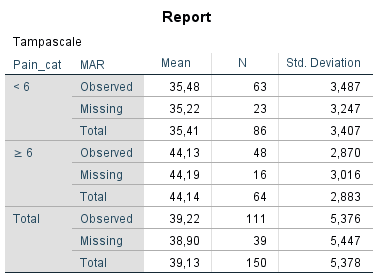
\includegraphics[width=0.9\linewidth]{images/tab2.3} 

}

\caption{MAR missing data in the Tampa scale variable.}\label{fig:tab2-3}
\end{figure}

\subsection{Missing Not At Random}\label{missing-not-at-random}

The data are MNAR when the probability of missing data in a variable is
related to the scores of that variable itself, e.g.~mostly high or low
scores are missing. In the LBP study, MNAR data can occur when patients
with the highest scores on the Tampa scale have missing Tampa scale
values. This is shown in the MNAR column of Figure \ref{fig:fig2-7}. The
MNAR column shows that the values that are most frequently missing are
for the patients with the highest Tampa scale scores, i.e.~for the
patients that fear their back problems most. A reason may be that these
patients were so afraid to move (which is assessed by the Tamp scale),
that they were not able to visit an assessment center. MNAR missing data
can also occur indirectly through the relationship of the variable with
missing data with another variable that is not available in the dataset.
For example, it could also be that patients with a high level of fear of
movement, worry a lot and therefore do not want to be confronted with
questions about their fear to move their back and therefore skip
questions of the Tampa scale. In case of a positive relationship between
worry and fear of movement, the highest values on the Tampa scale
variable are missing. If worry is not measured in the study, the missing
data in the Tampa scale variable is called MNAR. The difference with MAR
is that with MNAR, the missing data problem cannot be handled by the
observed variables in the dataset or by using a technique as Multiple
Imputation. However, as with MAR data, MNAR data can also not be
verified.

\subsection{The Missing Data
Indicator}\label{the-missing-data-indicator}

In the definitions of the missing data mechanisms in the previous
paragraphs we used the term probability several times, to indicate that
the relationship of variables with the probability of missingness in a
variable distinguishes the missing data mechanisms. The probability of
missing data can depend on other variables (MAR), on values of the
variables itself (MNAR) or nether of these (MCAR). Rubin proposed that
variables with missing data can be divided in a part that is observed
and a part that is missing. The observed and missing data can be coded
by a 0 and 1 respectively (\citet{Rubin1987}). In case of the Tampa
scale variable this means that the observed data is coded by a 0 and a 1
is used for the Tampa scale values that are missing. This dichotomous
coding variable is called the missing data indicator variable. Figure
\ref{fig:fig2-8} shows the missing data indicator variable for the
observed and missing data in the Tampa scale variable. This indicator
variable is now a single variable because there is missing data in only
the Tampa scale variable. When more variables contain missing data,
multiple indicator variables can be generated, one for each variable
that contains missing data.

\begin{figure}

{\centering 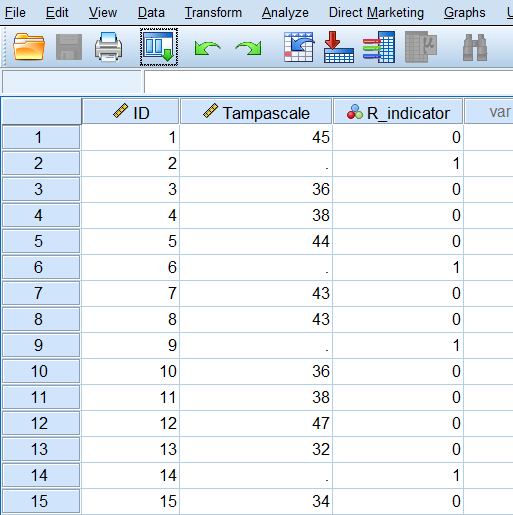
\includegraphics[width=0.9\linewidth]{images/fig2.8} 

}

\caption{The missing data in the Tampa scale variable coded according to the missing data indicator variable.}\label{fig:fig2-8}
\end{figure}

Using the missing data indicator variable implies that missing values
(or the probability of missing values) can be described by a statistical
model. This model may consist of variables that have a relationship with
the probability of missing data, in this case the indicator variable. A
logistic regression model can be used to describe the relationship of
variables with the probability of missing data in the Tampa scale
variable. Graphically these models can be visualized as displayed in
Figure 2.11 to 2.13 below. With logistic regression, the relationship of
a dichotomous outcome variable (i.e.~the missing data indicator
variable) with other variables can be described.

\begin{figure}

{\centering 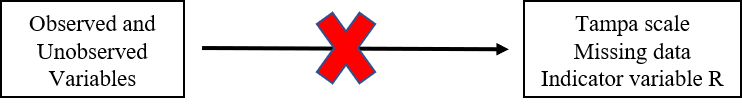
\includegraphics[width=0.9\linewidth]{images/fig2.9a} 

}

\caption{MCAR}\label{fig:fig2-9a}
\end{figure}

There is no relationship between, how the data became missing (indicated
by R) and observed and unobserved variables.

\begin{figure}

{\centering 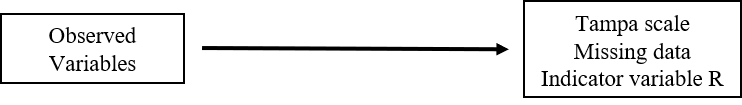
\includegraphics[width=0.9\linewidth]{images/fig2.9b} 

}

\caption{MAR}\label{fig:fig2-9b}
\end{figure}

There is a relationship between, how the data became missing (indicated
by R) and observed variables.

\begin{figure}

{\centering 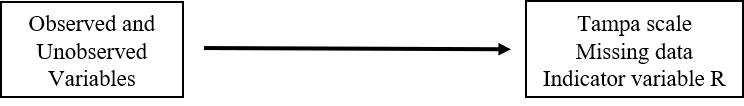
\includegraphics[width=0.9\linewidth]{images/fig2.9c} 

}

\caption{MNAR}\label{fig:fig2-9c}
\end{figure}

There is a relationship between, how the data got missing (indicated by
R) and observed and unobserved variables.

The missing data mechanisms of Rubin can then be described by the
following logistic regression functions, where \(R_{Tampa}\) indicates
the missing data indicator for the Tampa scale and \(\beta\) the
regression coefficient:

MCAR: No variables in or outside the dataset explain the missingness in
the Tampa scale variable, the model would be empty:
\[LN(\frac{R_{Tampa=1}}{1-R_{Tampa=1}}) = \beta_0\]

MAR: Variables in the dataset, like Pain and Radiation in the Leg
explain the missingness in the Tampa scale variable and the model would
be:
\[LN(\frac{R_{Tampa=1}}{1-R_{Tampa=1}}) = \beta_0 + \beta_1 * Pain + \beta_2 * Radiation\]

MNAR: Missingness in the Tampa scale variable can be explained by
variables in the dataset and by the score on the Tampa scale itself.

From these models we observe that the missing data models can be defined
by other observed variables in the dataset and/or missing data (which we
do not observe). It should be noted however, that we can never be
completely sure about the reason why data are missing. The above
mentioned relationships are therefore statistical relationships from
descriptive models and not from causal models. In summary, the MCAR
assumption is mostly very strict and not realistic in practice.The MAR
assumption is more realistic and mostly assumed in practice.The
difference bewteen MAR and MNAR is that in MNAR the probability of
missingness is also related to the unobserved (missing) data.

\subsection{The Role of Auxiliary
Variables}\label{the-role-of-auxiliary-variables}

Usually, the probability of missing data is related to other variables
and/or to the missing values itself (MAR or MNAR). Unfortunately, it is
not possible to distinguish between MAR and MNAR mechanisms, because the
missing values are unknown. Brand (\citet{Brand1999}) describes two
examples that demonstrate how an initially MNAR missing data mechanism
can change into MAR by including additional variables that are related
to the probability of missing data. Accordingly, by including variables
related to the probability of missing data a MNAR mechanism can get
closer to a MAR mechanism. The MAR assumption can be made more plausible
by including additional information in the missing data handling method
(\citet{Baraldi2010}). Therefore, it is advised, to include extra
variables that have a relationship with the missing data rate in other
variables, i.e.~have a relationship with the probability of missing data
or that have a relationship (correlated) with the variables that contain
the missing values (\citet{Collins2001}). These additional variables can
help dealing with missing data as well and are called auxiliary
variables.

\section{Missing Data evaluation}\label{missing-data-evaluation-1}

The performance of missing data methods depends on the underlying
missing data mechanism. As previously descirbed, the difference between
the MCAR and not-MCAR mechanisms depend on the relationship between the
probability for missing data and the observed variables. If this
relationship cannot be detected we assume that the data is MCAR. If
there is some kind of relationship, the missing data may be MAR or MNAR.
We can never distinguish between MAR or MNAR data, because for that we
need information about the missing values. Tests to distinguish the
missing data assumptions are therefore limited to accept or reject the
MCAR missing data assumption. In practice we study and measure outcomes
and independent variables that are related to each other. This makes the
MAR assumption mostly an accepted ``working'' missing data assumption in
practice.

There are two approaches to evaluate the missing data mechanism. First,
it is important to think about the most plausible reasons for the data
being missing. Researchers mostly have some possible explanation about
why data are missing and this information is very important. For
example, when during web based data collection, the internet is
sometimes disconnected, data of a few participants gets lost. When these
malfunctions are coincidental, it can be assumed that the missing data
are MCAR. However, when cognitive scores are assessed during this web
based data collection and these are mostly not filled out by people that
have decreased cognitive functions, the missing data can be assumed to
be MNAR. Second, statistical tests can be used to get an idea about the
missing data mechanism. In these statistical tests, the non-responders
(i.e., participants with missing observations), can be compared to the
responders on several characteristics. By doing this, we can test
whether the missing data mechanism is likely to be MCAR or not-MCAR
(because we cannot distinguish between MAR and MNAR missing data). There
are several possibilities to compare the non-responders with the
responders groups, for example using t-tests or Chi-square tests,
logistic regressions with the missing data indicator as the outcome, or
Little's MCAR test (\citet{Little1988}).

Researchers need to be aware that the assumptions that underlie an
independent t-test, logistic regression, and Chi-square test apply to
these missing data mechanism procedures as well. This means that the
residuals are assumed to be normally distributed and that the tests rely
on a decent sample size.

\subsection{Missing data Evaluation in
SPSS}\label{missing-data-evaluation-in-spss}

\subsubsection{Descriptive Statistics}\label{descriptive-statistics}

Descriptive information of variables can be obtained via the following
options of the Missing Value Analysis (MVA) module in the SPSS menu:

\begin{quote}
Analyze -\textgreater{} Missing Value Analysis\ldots{}
\end{quote}

Transfer all variables in the correct Quantitative and Categorical
variables window and then click

\begin{quote}
Descriptives option -\textgreater{} Univariate statistics
-\textgreater{} Continue.
\end{quote}

The following table will appear in the SPSS Output window.

\begin{figure}

{\centering 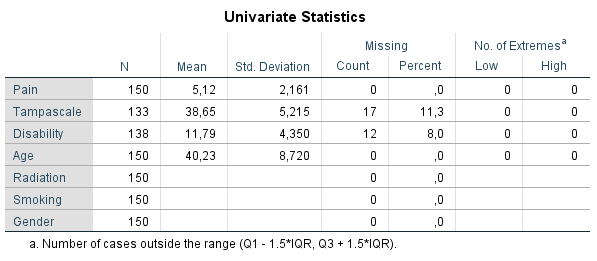
\includegraphics[width=0.9\linewidth]{images/tab2.4} 

}

\caption{Univariate descriptive statistics of variables with and without missing data.}\label{fig:tab2-4}
\end{figure}

Under the column N, the information of all cases in the dataset are
displayed. Further, for all continuous variables information about the
Mean and Standard deviation are displayed. No descriptive information is
given for categorical variables. Under the column Missing we get the
number and percentage of missing values in each variable and under the
column No. of Extremes we get information of cases that fall outside a
range, which is specified under the table. These descriptive information
of variables with missing data provide a quick overview of the amount of
missing data in each variable. However, it does not provide us
information about the relationship between variables with complete and
missing data and therefore does not give us an idea about the potential
missing data mechanism. Methods as T-tests, regression or Little's MCAR
test, discussed in the next section, can better be used for that
purpose.

\subsubsection{T-test procedure}\label{t-test-procedure}

For the t-test procedure, SPSS first separates cases with complete and
missing values by creating an indicator variable of variables that
ontain missing values. This can be all type of variables. Then, group
means of other (only continuous) variables are compared by using the
indicator variable as group variable within the t-test procedure. You
can apply his procedure by following:

\begin{quote}
Analyze -\textgreater{} Missing Value Analysis\ldots{} -\textgreater{}
Descriptives -\textgreater{} click ``t-tests with groups formed by
indicator variables'' and ``include probabilities in table''
-\textgreater{} Continue -\textgreater{} OK (Figure 2.15).
\end{quote}

\begin{figure}

{\centering 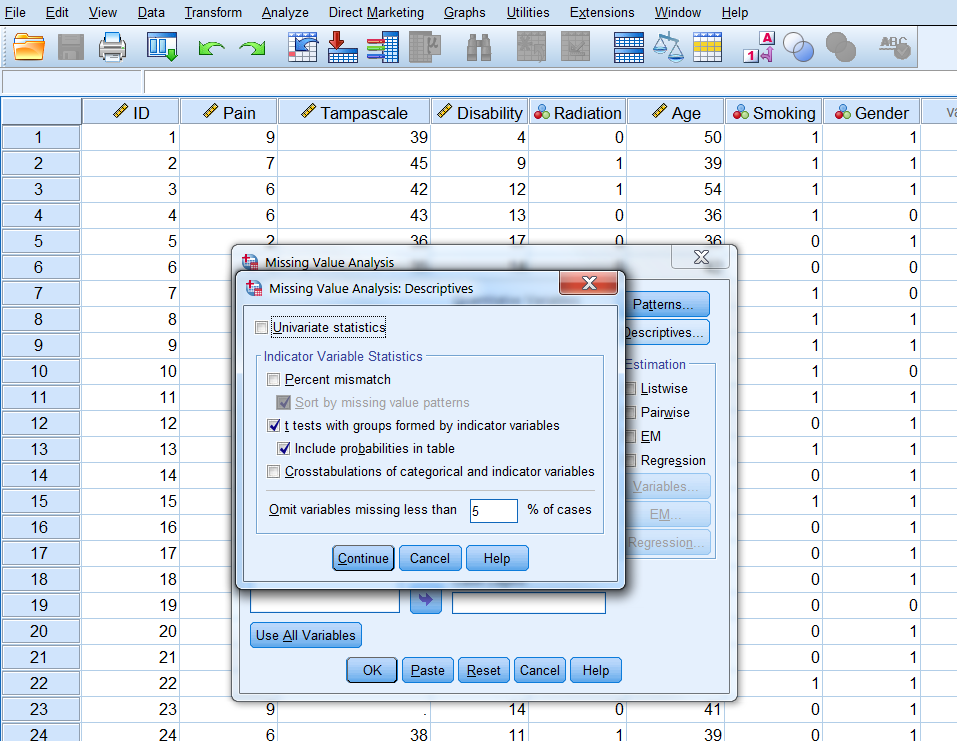
\includegraphics[width=0.9\linewidth]{images/fig2.11} 

}

\caption{The T-test procedure as part of the Missing Value Analysis menu}\label{fig:fig2-11}
\end{figure}

SPSS will produce the following table.

\begin{figure}

{\centering 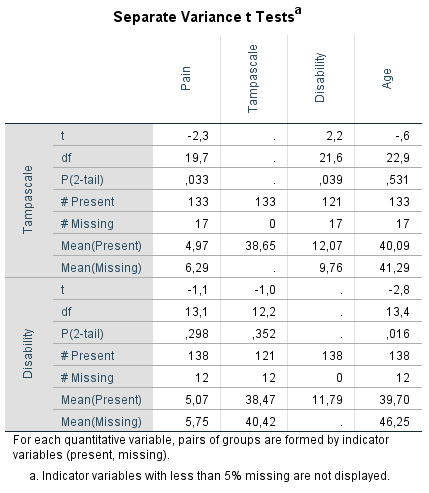
\includegraphics[width=0.7\linewidth]{images/tab2.5} 

}

\caption{Output table of the t-test procedure.}\label{fig:tab2-5}
\end{figure}

On the left side of the output table the names of the variables with
missing values are presented which are the Tampa scale and Disability
variables. Of these variables, indicator variables are defined which are
used to compare group means of other variables, that can be tested for
significance using independent t-tests. The results of these t-tests are
shown in the table according to the information in separate rows on the
left side with the t-value (t), degrees of freedom (df), P-value
(P(2-tail)), numbers of observed and missing cases (\# Present and \#
Missing) and means of observed and missing cases (Mean(Present) and
Mean(Missing)) presented. The variables for which the indicator groups
are compared, are listed in the columns of the table and are the Pain,
Tampa scale, Disability and Age variables. For the Tampa scale variable
that contain missing values, only the observed mean is presented,
because for the missing cases the values are missing. Note that in the
row of the Tampa scale variable the means of the Disability variable can
still be compared between the observed and missing cases, because they
do not miss values for exactly the same cases. Figure \ref{fig:tab2-5}
shows that patients that have observed values on the Tampa scale
variable (row Mean(Present)) differ significantly from patients with
missing values on the Tampa scale variable (row Mean(Missing)) on Pain
(P(2-tail = 0.033) and Disability (P(2-tail = 0.039). When we look at
the means of the Pain variable, we see that the mean of patients with
missing values on the Tampa scale variable is higher compared to the
mean of patients with observed scores. This means that there is a higher
probability of missing data on the Tampa scale variable for patients
with higher pain scores. If Tampa scale and Pain scores are correlated,
the missing values on the Tampa scale variable can also be explained by
the Pain score variable. This is also the case for the Age variable,
however, the t-test is not significant. For the Disability variable, it
is the other way around. We see more missing data on the Tampa scale
variable for lower Disability scores.

In the Missing Value Analysis and subsequently the descriptives option,
another possiblity is to select ``Crosstabulations of categorical and
indicator variables''. In that case a table is displayed to compare the
percentage of present and missing data for categorical variables related
to the indicator variable similarly defined as explained above. An
example can be found in Figure \ref{fig:tab2-8} that prodces SPSS when a
missing data indicator variable is used for the Radiation variable,
where for 11 cases data is missing.

\begin{figure}

{\centering 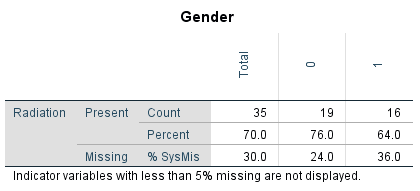
\includegraphics[width=0.7\linewidth]{images/Crosstabulation} 

}

\caption{Output table of the Crosstabulations procedure.}\label{fig:tab2-8}
\end{figure}

You see in the table that Radiation values are more frequently missing
for males (coded as 1 on the Gender variable) than for females (coded as
0). Note that for these tables, the Chi-square tests and p-values are
not performed. These have to be obtained via the usual Crosstabs
function, using a self-generated missing data indicator variable.

\subsubsection{Logistic Regression
Analysis}\label{logistic-regression-analysis}

The missing data mechanism can also be evaluated with a logistic
regression procedure (\citet{Ridout1991}). With logistic regression
analysis, we can evaluate if the probability of missing data is related
to other variables in the data. For this procedure, we first generate an
indicator variable that separates the subjects with missing values from
the participants with observed values. This indicator variable is used
as the dependent variable in a logistic regression analysis. A backward
regression can be used to determine the strongest predictors of missing
data. The output for the logistic regression with the Tampa scale
variable as the indicator outcome variable is presented in the table
below:

\begin{figure}

{\centering 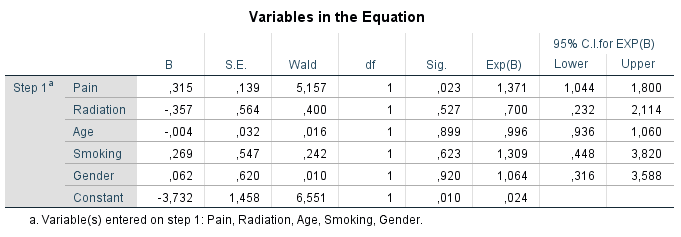
\includegraphics[width=0.9\linewidth]{images/tab2.6} 

}

\caption{Logistic regression analysis with variable that contain missing data as the outcome variable.}\label{fig:tab2-6}
\end{figure}

The variable Pain is significantly related to the missing data indicator
variable of the Tampa scale variable, which indicates that the
probability for missing data in the Tampa scale variable can be
explained by the Pain variable. The positive coefficient of 0.315
indicates that the probability of missing data on the Tampa scale
variable is higher for higher Pain scores. The other variables do not
show a significant relationship with missing data on the Tampa scale
variable. This logistic regression analysis procedure can be repeated
for each variable with missing values in the dataset.

\subsubsection{Little's MCAR test in
SPSS}\label{littles-mcar-test-in-spss}

Another possibility is to use a test that was developed by Roderick
Little: Little's MCAR test. This test is based on differences between
the observed and estimated means in each missing data pattern. This test
is developed for continuous data. We use it for the data in Figure
\ref{fig:fig2-1}. The test can be applied via:

\begin{quote}
Analyze -\textgreater{} Missing Value Analysis\ldots{}-\textgreater{}
select the continuous variables -\textgreater{} Select EM in the
Estimation group -\textgreater{} OK
\end{quote}

\begin{figure}

{\centering 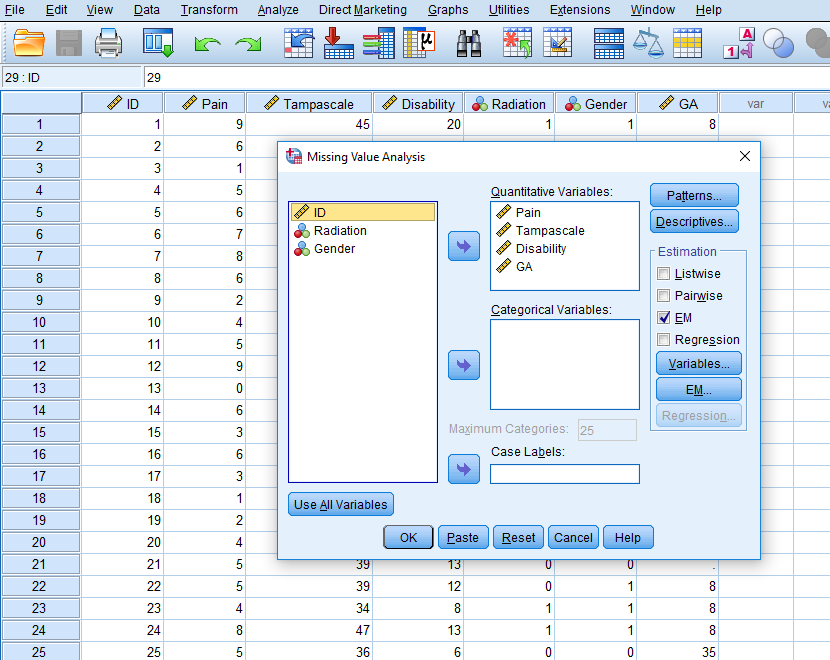
\includegraphics[width=0.9\linewidth]{images/fig2.12} 

}

\caption{EM selection in the Missing Value Analysis menu.}\label{fig:fig2-12}
\end{figure}

The following table that is called EM Means can be found in the output
window of SPSS. Under the table the result of Little's MCAR test is
displayed (tables that provide information of univariate statistics and
a summary of estimated means and standard deviations are also provided.
Further, tables that are called EM Covariances and EM Correlations are
also generated, but they provide the same results for Little's MCAR test
as under the EM Means table. These tables are not shown)

\begin{figure}

{\centering 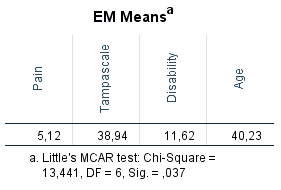
\includegraphics[width=0.6\linewidth]{images/tab2.7c} 

}

\caption{Output tables with information of Little’s MCAR test.}\label{fig:tab2-7}
\end{figure}

\subsection{Missing data Evaluation in
R}\label{missing-data-evaluation-in-r}

\subsubsection{Little's MCAR test in R}\label{littles-mcar-test-in-r}

Little´s MCAR test is available in the \texttt{BaylorEdPsych} package as
the \texttt{LittleMCAR} function. To apply the test, we select only the
continuous variables. We use it for the same dataset as in the previous
paragraph. The p-value for the test is not-siginificant, indicating that
the missings seem to be compeletely at random.

\begin{Shaded}
\begin{Highlighting}[]
\KeywordTok{library}\NormalTok{(haven)}
\NormalTok{dataset <-}\StringTok{ }\KeywordTok{read_sav}\NormalTok{(}\StringTok{"data/CH2 example.sav"}\NormalTok{)}
\KeywordTok{library}\NormalTok{(BaylorEdPsych)}
\KeywordTok{LittleMCAR}\NormalTok{(dataset[,}\KeywordTok{c}\NormalTok{(}\StringTok{"Pain"}\NormalTok{, }\StringTok{"Tampascale"}\NormalTok{,}\StringTok{"Disability"}\NormalTok{, }\StringTok{"GA"}\NormalTok{)])}
\end{Highlighting}
\end{Shaded}

\begin{verbatim}
## this could take a while
\end{verbatim}

\begin{verbatim}
## $chi.square
## [1] 0.7537406
## 
## $df
## [1] 3
## 
## $p.value
## [1] 0.8604966
## 
## $missing.patterns
## [1] 2
## 
## $amount.missing
##                 Pain Tampascale Disability  GA
## Number Missing     0          0          0 5.0
## Percent Missing    0          0          0 0.1
## 
## $data
## $data$DataSet1
##    Pain Tampascale Disability GA
## 1     9         45         20  8
## 2     6         43         10 36
## 3     1         36          1  8
## 5     6         44         14  8
## 6     7         43         11 29
## 8     6         43         11 34
## 9     2         37         11  8
## 10    4         36          3 38
## 11    5         38         16  8
## 12    9         47         14  8
## 13    0         32          3 42
## 14    6         38         12  8
## 15    3         34         13 39
## 17    3         35         11 26
## 18    1         31          1  8
## 19    2         31          7  8
## 20    4         32          9 28
## 22    5         39         12  8
## 23    4         34          8  8
## 24    8         47         13  8
## 25    5         36          6 35
## 26    5         38         16  8
## 27    9         48         23  8
## 28    3         36          3 36
## 30    6         37         16 40
## 31   10         43         21  8
## 32    4         37          8 39
## 33   10         42         20  8
## 34    2         37          3 37
## 35    6         43         12  8
## 36    3         38          7  8
## 37    8         47          8 35
## 38    3         38          6  8
## 39    3         39          8 33
## 40    7         44         15  8
## 41    7         45         10 32
## 42    6         40         12  8
## 43    7         40         16  8
## 44    1         35          2 34
## 45    9         41         19  8
## 46    5         41         17 38
## 47    6         43         11 41
## 48    3         39          9 33
## 49    2         33          6  8
## 50    8         44         19 32
## 
## $data$DataSet2
##    Pain Tampascale Disability GA
## 4     5         38         14 NA
## 7     8         43         18 NA
## 16    6         42          8 NA
## 21    5         39         13 NA
## 29    2         36          9 NA
\end{verbatim}

\chapter{Single Missing data
imputation}\label{single-missing-data-imputation}

The topic of this Chapter is to explain how simple missing data methods
like complete case analysis, mean and single regression imputation work.
These procedures are still very often applied \citep{Eekhout2012} but
generally not recommended because they decreases statistical power or
lead to an incorrect estimation of standard errors when the data is
MCAR, MAR and MNAR
\citep{Eekhout2014, VanBuuren2018, enders2010applied}.

We use as an example data from a study about low back pain and we want
to study if the Tampa scale variable is a predictor of low back pain.
Both variables are continuous. Pain represents the intensity of the low
back pain and the Tampa scale measures fear of moving the low back. The
Tampa scale variable contains missing values. The number or type of
missing values is not important because the main topic is to show how
simple missing data methods work in SPSS and R.

To get a first impression about the relationship between the Pain and
the Tampa scale variables we make a scatterplot. The scatterplots with
the complete and intended incomplete data is displayed in Figure
\ref{fig:fig3-1}.

\begin{figure}

{\centering 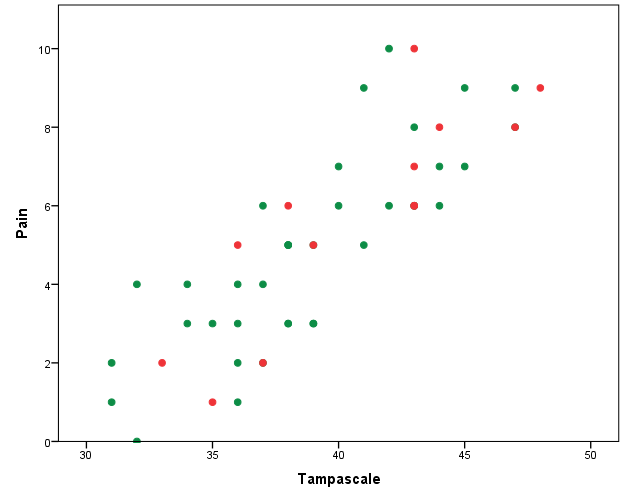
\includegraphics[width=0.7\linewidth]{images/fig3.2a} 

}

\caption{Relationship between the Tampa scale and Pain variables (green dots are observed and red dots are the missing data}\label{fig:fig3-1}
\end{figure}

The green dots in Figure 3.1 represent the observed data and the red
dots the missing data points. In practice, you work with the available
points that are visualized in Figure \ref{fig:fig3-2}.

\begin{figure}

{\centering 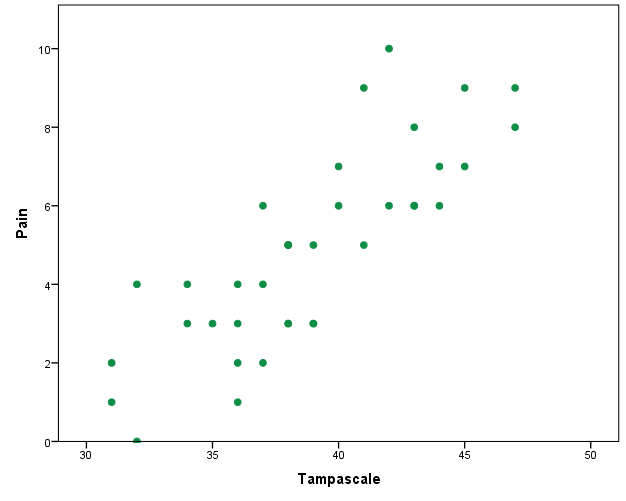
\includegraphics[width=0.7\linewidth]{images/fig3.2b} 

}

\caption{Relationship between the Tampa scale and Pain variable. Missing data are excluded}\label{fig:fig3-2}
\end{figure}

\section{Complete cases analysis}\label{complete-cases-analysis}

Complete case analysis (CCA) means that persons with a missing data
point are excluded from the dataset before statistical analyses are
performed. Nevertheless it is the default procedure in many statistical
software packages such as SPSS.

\section{Mean Imputation}\label{mean-imputation}

With mean imputation the mean of a variable that contains missing values
is calculated and used to replace all missing values in that variable.

\subsection{Mean imputation in SPSS}\label{mean-imputation-in-spss}

\emph{Descriptive Statistics}

The easiest method to do mean imputation is by calculating the mean
using

\begin{quote}
Analyze -\textgreater{} Descriptive Statistics -\textgreater{}
Descriptives
\end{quote}

and than replace the missing values by the mean value by using the
``Recode into Same Variables''under the Transform menu.

Other procedures for mean imputation are the \emph{Replace Missing
Values} procedure under Transform and by using the \emph{Linear
Regression} procedure.

\emph{Replace Missing Values procedure}

You can find the Replace Missing Values dialog box via

\begin{quote}
Transform -\textgreater{} Replace Missing Values.
\end{quote}

A new window opens. Transport the Tampa scale variable to the New
variable(s) window (Figure \ref{fig:fig3-3}). The default imputation
procedure is Mean imputation or called ``Series mean''.

\begin{figure}

{\centering 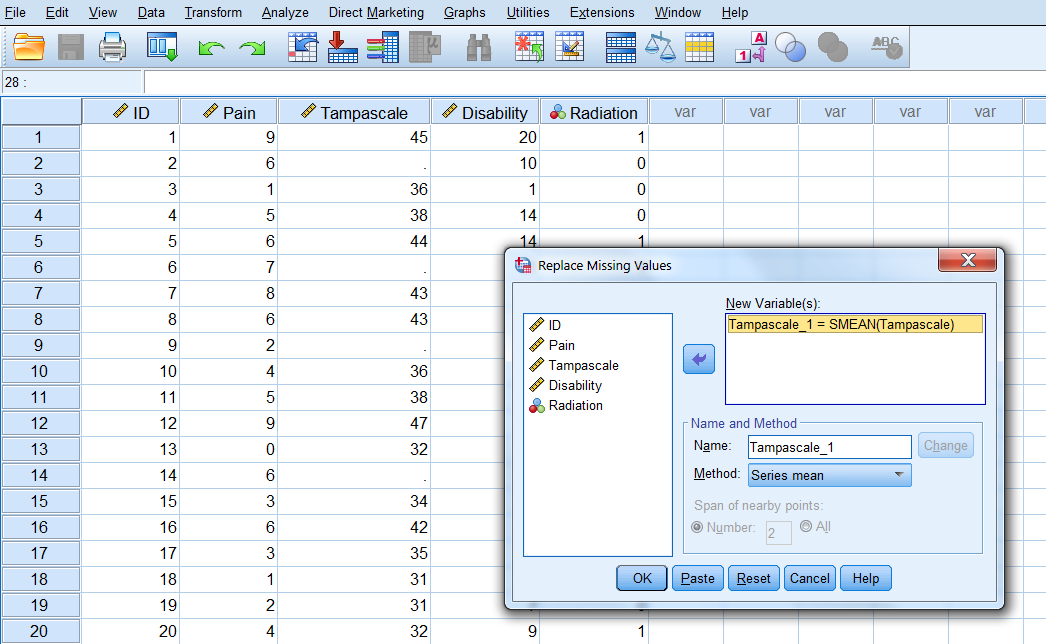
\includegraphics[width=0.7\linewidth]{images/fig3.6} 

}

\caption{Window for mean imputation of the Tampa scale variable.}\label{fig:fig3-3}
\end{figure}

When you click on OK, a new variable is created in the dataset using the
existing variable name followed by an underscore and a sequential
number. The result is shown in Figure \ref{fig:fig3-7}.

\begin{figure}

{\centering \includegraphics[width=0.7\linewidth]{images/fig3.7} 

}

\caption{Mean imputation of the Tampa scale variable with the Replace Missing Values procedure.}\label{fig:fig3-7}
\end{figure}

If we now make the scatterplot between the Pain and the Tampa scale
variable it clearly shows the result of the mean imputation procedure,
all imputed values are located at the mean value (Figure
\ref{fig:fig3-4}).

\begin{figure}

{\centering \includegraphics[width=0.7\linewidth]{images/fig3.4} 

}

\caption{Scatterplot between the Tampa scale and Pain variable, after the missing values of the Tampa scale variable have been replaced by the mean.}\label{fig:fig3-4}
\end{figure}

\emph{Linear Regression}

Mean imputation is also integrated in the Linear Regression menu via:

\begin{quote}
Analyze -\textgreater{} Regression -\textgreater{} Linear
-\textgreater{} Options.
\end{quote}

In the Missing Values group you choose for Replace with mean (Figure
\ref{fig:fig3-8}).

\begin{figure}

{\centering \includegraphics[width=0.7\linewidth]{images/fig3.8} 

}

\caption{The option Replace with mean in the Linear Regression menu.}\label{fig:fig3-8}
\end{figure}

\subsection{Mean imputation in R}\label{mean-imputation-in-r}

You can do mean imputation by using the mice function in the mice
package and choose as method ``mean''.

\begin{Shaded}
\begin{Highlighting}[]
\KeywordTok{library}\NormalTok{(foreign) }\CommentTok{# activate the foreign package to use the read.spss function}
\NormalTok{dataset <-}\StringTok{ }\KeywordTok{read.spss}\NormalTok{(}\DataTypeTok{file=}\StringTok{"Backpain 50 missing.sav"}\NormalTok{, }\DataTypeTok{to.data.frame=}\NormalTok{T)}
\end{Highlighting}
\end{Shaded}

\begin{verbatim}
## re-encoding from UTF-8
\end{verbatim}

\begin{Shaded}
\begin{Highlighting}[]
\KeywordTok{library}\NormalTok{(mice) }\CommentTok{# Activate the mice package to use the mice function}
\NormalTok{imp_mean <-}\StringTok{ }\KeywordTok{mice}\NormalTok{(dataset, }\DataTypeTok{method=}\StringTok{"mean"}\NormalTok{, }\DataTypeTok{m=}\DecValTok{1}\NormalTok{, }\DataTypeTok{maxit=}\DecValTok{1}\NormalTok{)}
\end{Highlighting}
\end{Shaded}

\begin{verbatim}
## 
##  iter imp variable
##   1   1  Tampascale
\end{verbatim}

You can extract the mean imputed dataset by using the complete function
as follows: \texttt{complete(imp\_mean)}

\section{Regression imputation}\label{regression-imputation}

With regression imputation the information of other variables is used to
predict the missing values in a variable by using a regression model.
Commonly, first the regression model is estimated in the observed data
and subsequently using the regression weights the missing values are
predicted and replaced.

\subsection{Regression imputation in
SPSS}\label{regression-imputation-in-spss}

You can apply regression imputation in SPSS via the Missing Value
Analysis menu. There are two options for regression imputation, the
Regression option and the Expectation Maximization (EM) option. The
Regression option in SPSS has some flaws in the estimation of the
regression parameters \citep{hippel2004}. Therefore, we recommend the EM
algorithm. This algorithm is a likelihood-based procedure. This means
that the most likely values of the regression coefficients are estimated
given the data and subsequently used to impute the missing value. This
EM procedure gives the same results as first performing a simple
regression analysis in the dataset and subsequently estimate the missing
values from the regression equation. Both methods are described below.

\subsubsection{EM procedure}\label{em-procedure}

Step 1, go to:

\begin{quote}
Analyze -\textgreater{} Missing Value Analysis\ldots{}
\end{quote}

In the main Missing Value Analysis dialog box, select the variable(s)
and select EM in the Estimation group (Figure \ref{fig:fig3-10}).

\begin{figure}

{\centering \includegraphics[width=0.7\linewidth]{images/fig3.10} 

}

\caption{EM Selection in the Missing Value Analysis window.}\label{fig:fig3-10}
\end{figure}

Step 2 click Variables, to specify predicted and predictor variables.
Place the Tampascale variable in the Predicted variables window and the
Pain variable in the Predictor Variables window (Figure
\ref{fig:fig3-11}).

\begin{figure}

{\centering \includegraphics[width=0.7\linewidth]{images/fig3.11} 

}

\caption{Transfer of the Tampascale and Pain variables to the Predicted and Predictor Variables windows.}\label{fig:fig3-11}
\end{figure}

Step 3 Click on Continue -\textgreater{} EM and select Normal in the
Distribution group. Than thick Save completed data and give the dataset
a name, for example ``ImpTampa\_EM'' (Figure \ref{fig:fig3-12}).

\begin{figure}

{\centering \includegraphics[width=0.7\linewidth]{images/fig3.12} 

}

\caption{Name of dataset to save the EM results in.}\label{fig:fig3-12}
\end{figure}

Step 4 Click Continue -\textgreater{} OK. The new dataset
``ImpTampa\_EM'' will open in a new window in SPSS. In this dataset the
imputed data for the Tampascale Variable together with the original data
is stored (Figure \ref{fig:fig3-13}, first 15 patients are shown).

\begin{figure}

{\centering \includegraphics[width=0.7\linewidth]{images/fig3.13} 

}

\caption{Result of the EM procedure.}\label{fig:fig3-13}
\end{figure}

BNote that SPSS uses as default only quantitative variables to impute
the missing values with the EM algorithm.

\subsubsection{Normal Linear Regression
imputation}\label{normal-linear-regression-imputation}

We first estimate the relationship between Pain and the Tampa scale
variable in the dataset with linear regression, by default subjects with
missing values are excluded. Subsequently, we use the regression
coefficients from this regression model to estimate the imputed values
in the Tampa scale variable.

To estimate the linear regression model, choose:

\begin{quote}
Analyze -\textgreater{} Regression -\textgreater{} Linear
\end{quote}

Transfer the Tampa scale variable to the Dependent variable box and the
Pain variable to the ``Independent(s) in the Block 1 of 1 group. Then
click OK.

\begin{figure}

{\centering \includegraphics[width=0.7\linewidth]{images/fig3.14} 

}

\caption{Linear regression analysis with the Tampa scale as the outcome and Pain as the independent variable.}\label{fig:fig3-14}
\end{figure}

\begin{figure}

{\centering \includegraphics[width=0.7\linewidth]{images/table3.3} 

}

\caption{Result of the linear regression analysis.}\label{fig:tab3-3}
\end{figure}

The linear regression model can be described as:

\[Tampascale = 32.005 + 1.410 × Pain\]

Now impute the missing values in the Tampa scale variable and compare
them with the EM estimates. You see that the results are the same.

\begin{figure}

{\centering \includegraphics[width=0.7\linewidth]{images/fig3.15} 

}

\caption{Predictions of the missing Tampa scale values on basis of the regression model estimated in the dataset after the missing values were excluded.}\label{fig:fig3-15}
\end{figure}

In the scatterplot of the imputations from the regression model you see
that, as expected, the imputed values are directly on the regression
line (Figure \ref{fig:fig3-16}).

\begin{figure}

{\centering \includegraphics[width=0.7\linewidth]{images/fig3.16} 

}

\caption{Relationship between the Tampa scale and the Pain variable.}\label{fig:fig3-16}
\end{figure}

\subsection{Regression imputation in
R}\label{regression-imputation-in-r}

You can aply regression imputation in R with as method setting
``norm.predict'' in the mice function. The Pain variable is used to
predict the missing values in the Tampa scale variable.

\begin{Shaded}
\begin{Highlighting}[]
\KeywordTok{library}\NormalTok{(foreign)}
\NormalTok{dataset <-}\StringTok{ }\KeywordTok{read.spss}\NormalTok{(}\DataTypeTok{file=}\StringTok{"Mean imputation.sav"}\NormalTok{, }\DataTypeTok{to.data.frame=}\NormalTok{T)}
\end{Highlighting}
\end{Shaded}

\begin{verbatim}
## re-encoding from UTF-8
\end{verbatim}

\begin{Shaded}
\begin{Highlighting}[]
\NormalTok{dataset <-}\StringTok{ }\NormalTok{dataset[, }\KeywordTok{c}\NormalTok{(}\StringTok{"Pain"}\NormalTok{, }\StringTok{"Tampascale"}\NormalTok{)]}

\NormalTok{imp.regress <-}\StringTok{ }\KeywordTok{mice}\NormalTok{(dataset, }\DataTypeTok{method=}\StringTok{"norm.predict"}\NormalTok{, }\DataTypeTok{m=}\DecValTok{1}\NormalTok{, }\DataTypeTok{maxit=}\DecValTok{1}\NormalTok{)}
\end{Highlighting}
\end{Shaded}

\begin{verbatim}
## 
##  iter imp variable
##   1   1  Tampascale
\end{verbatim}

\begin{Shaded}
\begin{Highlighting}[]
\NormalTok{imp.regress}\OperatorTok{$}\NormalTok{imp}\OperatorTok{$}\NormalTok{Tampascale }\CommentTok{# Extract the imputed values}
\end{Highlighting}
\end{Shaded}

\begin{verbatim}
##           1
## 2  40.46554
## 6  41.87566
## 9  34.82506
## 14 40.46554
## 21 39.05542
## 25 39.05542
## 27 44.69590
## 31 46.10602
## 35 40.46554
## 37 43.28578
## 44 33.41494
## 49 34.82506
## 50 43.28578
\end{verbatim}

Expectantly, this gives comparable results as the regression imputation
to SPSS above. The method ``norm.predict'' in the mice package fits a
linear regression model in the dataset and generates the imputed values
for the Tampa scale variable by using the regression coefficients of the
linear regression model. The completed dataset can be extracted by using
the complete function in the mice package.

\subsection{Stochastic regression
imputation}\label{stochastic-regression-imputation}

In Stochastic regression models imputation uncertainty is accounted for
by adding extra error variance to the predicted values from the linear
regression model. Stochastic regression can be activated in SPSS via the
Missing Value Analysis and the Regression Estimation option. However,
the Regression Estimation option generates incorrect regression
coefficient estimates \citep{hippel2004} and will therefore not further
discussed.

\subsection{Stochastic regression imputation in
R}\label{stochastic-regression-imputation-in-r}

You can apply stochastic regression imputation in R with the mice
function using the method ``norm.nob''.

\begin{Shaded}
\begin{Highlighting}[]
\NormalTok{dataset <-}\StringTok{ }\KeywordTok{read.spss}\NormalTok{(}\DataTypeTok{file=}\StringTok{"Backpain 50 missing.sav"}\NormalTok{, }\DataTypeTok{to.data.frame=}\NormalTok{T)}
\end{Highlighting}
\end{Shaded}

\begin{verbatim}
## re-encoding from UTF-8
\end{verbatim}

\begin{Shaded}
\begin{Highlighting}[]
\NormalTok{dataset <-}\StringTok{ }\NormalTok{dataset[, }\KeywordTok{c}\NormalTok{(}\StringTok{"Pain"}\NormalTok{, }\StringTok{"Tampascale"}\NormalTok{)]}

\NormalTok{imp_nob <-}\StringTok{ }\KeywordTok{mice}\NormalTok{(dataset, }\DataTypeTok{method=}\StringTok{"norm.nob"}\NormalTok{, }\DataTypeTok{m=}\DecValTok{1}\NormalTok{, }\DataTypeTok{maxit=}\DecValTok{1}\NormalTok{)}
\end{Highlighting}
\end{Shaded}

\begin{verbatim}
## 
##  iter imp variable
##   1   1  Tampascale
\end{verbatim}

The completed dataset can be extracted by using the complete function in
the mice package.

\section{Bayesian Stochastic regression
imputation}\label{bayesian-stochastic-regression-imputation}

With Bayesian Stochastic regression imputation uncertainty is not only
accounted for by adding error variance to the predicted values but also
by taking into account the uncertainty in estimating the regression
coefficients of the imputation model. The Bayesian idea is used that
there is not one (true) population regression coefficient but that the
regression coefficients itself follows a distribution. For more
information about the theory of Bayesian statistics we refer to the
books of
\citep{box2007bayesianinferencein, enders2010applied, gelman2014bayesian}.

\subsection{Bayesian Stochastic regression imputation in
SPSS}\label{bayesian-stochastic-regression-imputation-in-spss}

In SPSS Bayesian Stochastic regression imputation can be performed via
the multiple imputation menu. To generate imputations for the Tampa
scale variable, we use the Pain variable as the only predictor.

\textbf{Step 1}

To start the imputation procedure, Go to

\begin{quote}
Analyze -\textgreater{} Multiple Imputation -\textgreater{} Impute
Missing Data Values.
\end{quote}

In the first window you define which variables are included in the
imputation model. Transfer the Tampa scale and Pain variable to the
Variables in Model box. Than set the number of imputed datasets to 1
under Imputations and give the dataset where the imputed values are
stored under ``Create a new dataset'' a name. Here we give it the name
``ImpStoch\_Tampa'' (Figure \ref{fig:fig3-18}).

\begin{figure}

{\centering \includegraphics[width=0.7\linewidth]{images/fig3.18} 

}

\caption{The Variables window.}\label{fig:fig3-18}
\end{figure}

\textbf{Step 2}

In the Methods tab, choose under Imputation Method for custom and then
Fully conditional specification (MCMC). Set the Maximum iterations
number at 50. This specifies the number of iterations as part of the FCS
method (Figure \ref{fig:fig3-19}). We further use the default settings.

\begin{figure}

{\centering \includegraphics[width=0.7\linewidth]{images/fig3.19} 

}

\caption{The Methods tab.}\label{fig:fig3-19}
\end{figure}

\textbf{Step 3}

In the constraints window (Figure \ref{fig:fig3-20}) click on the Scan
Data button and further use the default settings.

\begin{figure}

{\centering \includegraphics[width=0.7\linewidth]{images/fig3.20} 

}

\caption{Bayesian Stochastic regression imputation}\label{fig:fig3-20}
\end{figure}

\textbf{Step 4}

In the Output window we only use the default settings.

\begin{figure}

{\centering \includegraphics[width=0.7\linewidth]{images/fig3.21} 

}

\caption{The Output tab.}\label{fig:fig3-21}
\end{figure}

\textbf{Step 5}

Now click on OK button to start the imputation procedure

The output dataset consists of the original data with missing data plus
a set of cases with imputed values for each imputation. The imputed
datasets are stacked under each other. The file also contains a new
variable, Imputation\_, which indicates the number of the imputed
dataset (0 for original data and more than 0 for the imputed datasets).
The variable Imputation\_ is added to the dataset and the imputed values
are marked yellow.

\begin{figure}

{\centering \includegraphics[width=0.7\linewidth]{images/fig3.22} 

}

\caption{Imputed dataset.}\label{fig:fig3-22}
\end{figure}

\begin{figure}

{\centering \includegraphics[width=0.7\linewidth]{images/fig3.23} 

}

\caption{Imputed dataset with the imputed values marked yellow.}\label{fig:fig3-23}
\end{figure}

When we make a scatterplot of the Pain and the Tampascale variable
(Figure \ref{fig:fig3-24}) we see that there is more variation in the
Tampascale variable, or you could say that the variation in the
Tampascale variable is ``repaired''.

\begin{figure}

{\centering \includegraphics[width=0.7\linewidth]{images/Fig3.24} 

}

\caption{Scatterplot of the relationship between Tampascale and the Pain variable, including the imputed values for the Tampascale variable (red dots).}\label{fig:fig3-24}
\end{figure}

The full Multiple Imputation procedure will be discussed in more detail
in the next Chapter.

\subsection{Bayesian Stochastic regression imputation in
R}\label{bayesian-stochastic-regression-imputation-in-r}

The package mice also include a Bayesian stochastic regression
imputation procedure. You can apply this imputation procedure with the
mice function and use as method ``norm''. The pain variable is the only
predictor variable for the missing values in the Tampa scale variable.

\begin{Shaded}
\begin{Highlighting}[]
\KeywordTok{library}\NormalTok{(haven)}
\NormalTok{dataset <-}\StringTok{ }\KeywordTok{read_sav}\NormalTok{(}\DataTypeTok{file=}\StringTok{"Backpain 50 missing.sav"}\NormalTok{)}
\NormalTok{dataset <-}\StringTok{ }\NormalTok{dataset[, }\KeywordTok{c}\NormalTok{(}\StringTok{"Pain"}\NormalTok{, }\StringTok{"Tampascale"}\NormalTok{)]}

\NormalTok{imp_b <-}\StringTok{ }\KeywordTok{mice}\NormalTok{(dataset, }\DataTypeTok{method=}\StringTok{"norm"}\NormalTok{, }\DataTypeTok{m=}\DecValTok{1}\NormalTok{, }\DataTypeTok{maxit=}\DecValTok{1}\NormalTok{)}
\end{Highlighting}
\end{Shaded}

\begin{verbatim}
## 
##  iter imp variable
##   1   1  Tampascale
\end{verbatim}

The completed dataset can be extracted by using the \texttt{complete}
function in the \texttt{mice} package.

\part{Part III: Multiple
Imputation}\label{part-part-iii-multiple-imputation}

\chapter{Multiple Imputation}\label{multiple-imputation}

In this Chapter we discuss an advanced missing data handling method,
Multiple Imputation (MI). With MI, each missing value is replaced by
several different values and consequently several different completed
datasets are generated. The concept of MI can be made clear by the
following figure \ref{fig:fig4-1}.

\begin{figure}

{\centering \includegraphics[width=0.9\linewidth]{images/fig4.1} 

}

\caption{Graphical presentation of the MI procedure.}\label{fig:fig4-1}
\end{figure}

In the first step, the dataset with missing values (i.e.~the incomplete
dataset) is copied several times. Then in the next step, the missing
values are replaced with imputed values in each copy of the dataset. In
each copy, slightly different values are imputed due to random
variation. This results in mulitple imputed datasets. In the third step,
the imputed datasets are each analyzed and the study results are then
pooled into the final study result. In this Chapter, the first phase in
multiple imputation, the imputation step, is the main topic. In the next
Chapter, the analysis and pooling phases are discussed.

\section{Multivariate Imputation by Chained
Equations}\label{multivariate-imputation-by-chained-equations}

Multivariate imputation by chained equations (MICE)
\citep{VanBuuren2018} is also known as Sequential Regression Imputation,
Fully Conditional Specification or Gibbs sampling. In the MICE
algorithm, a chain of regression equations is used to obtain
imputations, which means that variables with missing data are imputed
one by one. The regression models use information from all other
variables in the model, i.e.~conditional imputation models. In order to
add sampling variability to the imputations, residual error is added to
create the imputed values. This residual error can either be added to
the prediced values directly, which is esentially similar to repeating
stochastic regression imputation over several imputation runs. Or, the
residual variance can be added via the parameter estimates of the
regression model, which is a Bayesian sampling method. The Bayesian
method is the default in the \texttt{mice} package in R. The MICE
procedure became available in SPSS when version 17 was released.

\section{Multiple imputation in SPSS}\label{multiple-imputation-in-spss}

The MI procedure in SPSS is based on the MICE algorithm that was
developed in R. It is therefore no surprise that most options of the
mice function in R are also available in SPSS. Note that before you
start the MI procedure it is important to set the measurement level of
the variables with missing data in the Variable View window of your
data. They are important for the regression model that is used to
estimate the missing values in that variable. For example, if you define
a variable as scale, then linear regression models are used, for
categorical variables, logistic regression models are used.

We use as an example a dataset with 50 patient with low back pain. In
these patients information was measured about their Pain, Tampa scale,
Disability and Radiation. The variables Tampa scale and Disability
contain missing values of 26\% and 18\% respectively.

The multiple imputation procedure is started by navigating to

\begin{quote}
Analyze -\textgreater{} Multiple Imputation -\textgreater{} Impute
Missing Data Values.
\end{quote}

Than a window opens that consists of 4 tabs, a Variables, a Method, a
Constraints and an Output tab. You have to visit these tabs to specify
the imputation settings before you can start the imputation process by
clicking the OK button.

\begin{figure}

{\centering \includegraphics[width=0.9\linewidth]{images/fig4.6} 

}

\caption{The variables Tab}\label{fig:fig4-6}
\end{figure}

The first window is the Variables tab (Figure \ref{fig:fig4-6}). Here
you can transport the complete and incomplete variables that you want to
include in the imputation model to the window ``Variables in Model''.
The variables are imputed sequentially in the order in which they are
listed in the variables list. These variables are here Pain, Tampa
scale, Disability and Radiation. In our example the Tampa scale variable
is imputed before the Disability variable because the Tampa scale
variable was first listed. Further, the number of imputed datasets can
be defined in the ``Imputations''" box, we choose 5 here. Than you go to
``Create a new Dataset'' and choose a name for the dataset to which the
imputed data values are saved, which is called ``LBP\_Imp''. If you are
finished you visit the Methods Tab where you can define the imputation
method.

\begin{figure}

{\centering \includegraphics[width=0.9\linewidth]{images/fig4.7} 

}

\caption{The Methods Tab}\label{fig:fig4-7}
\end{figure}

In the Method tab (Figure \ref{fig:fig4-7}) you choose the imputation
algorithm. We choose for ``Custom'' under Imputation Method and for
Fully conditional specification (FCS). FCS is the Bayesian regression
imputation method as explained in \emph{Chapter 3}. You can also change
the maximum number of Iterations which has a default setting of 10. It
is recommended to increase that number to 50. Under Model type for scale
(continuous) variables we choose for Predictive Mean Matching (PMM) (see
paragraph 4.6 for a more detailed explanation of PMM). PMM is the
default procedure in the \texttt{mice} package to impute continuous
variables. In SPSS the default is the linear regression procedure. It is
better to change it into PMM. Now visit the Constraints Tab.

\begin{figure}

{\centering \includegraphics[width=0.9\linewidth]{images/fig4.8} 

}

\caption{The Constraints Tab}\label{fig:fig4-8}
\end{figure}

In the Constraints tab (Figure \ref{fig:fig4-8}) the role of variables
during the imputation process can be defined. For example, it is
possible to restrict the range of imputed values of a scale variable
when for scale variables the Linear Regression model was chosen in the
Method tab. To obtain the current range of variable values you can click
on the ``Scan'' button. When the PMM method is selected in the Method
Tab, the Constraints tab can be skipped. You can also restrict the
analysis to variables with less than a maximum percentage of missing
values when you select ``Exclude variables with large amounts of missing
data''. Finally, in the Output Tab the generated output can be selected.

\begin{figure}

{\centering \includegraphics[width=0.9\linewidth]{images/fig4.9} 

}

\caption{The Output Tab}\label{fig:fig4-9}
\end{figure}

In the Output tab (Figure \ref{fig:fig4-9}) descriptive statistics of
variables that are imputed can be exctracted by selecting ``Imputation
model'' and ``the Descriptive statistics for variables with imputed
values'' options. You can also request a dataset that contains iteration
history data, which we name ``Iter\_Backpain''. The dataset contains the
means and standard deviations of the imputed scale variables at each
iteration. You can use this data to check for irregularities during
imputation by making convergence plot that will be discussed in
paragraph 4.5.

\section{Random number generator}\label{random-number-generator}

Before you start the multiple imputation procedure, it is possible to
set the starting point of the random number generator in SPSS at a fixed
value of 950 (in R we use the seed for this). In this way you are able
to reproduce results exactly. later. It is also a good idea to store the
multiple imputed datasets.

We set the random number generator in SPSS via

\begin{quote}
Transform -\textgreater{} Random Number Generators -\textgreater{} Set
Starting point -\textgreater{} Fixed Value
\end{quote}

\begin{figure}

{\centering \includegraphics[width=0.7\linewidth]{images/fig4.5} 

}

\caption{Set the Random Number Generator }\label{fig:fig4-5}
\end{figure}

\section{The output for Multiple imputation in
SPSS}\label{the-output-for-multiple-imputation-in-spss}

\subsection{The Imputed datasets}\label{the-imputed-datasets}

After multiple imputation, the multiple imputed datasets are stored in a
new SPSS file and are stacked on top of each other. A new variable that
is called \texttt{Imputation\_} is added to the dataset and can be found
in the first column. This Imputation\_ variable is a nominal variable
that separates the original from the imputed datasets. This is also
indicated in the corner on the right side below in the Data View and
Variable View windows by the note ``Split by imputation\_''. You can
compare the use of this variable with the Split File option in SPSS
where all analyses are done separately for the categories of the
variable used to split the analyses. The difference is that with the
\texttt{Imputation\_} variable you also obtain pooled estimates for the
statistical analyses. When missing values are imputed with any another
software program, and you read in the imputed data in SPSS and add an
\texttt{Imputation\_} variable yourself the data is recognized by SPSS
as multiple imputed data. The imputed values are marked yellow. By these
marking SPSS recognized the dataset as an (multiple) imputed dataset
which is important for further statistical analyses (see Chapter 5,
paragraph 5.1)

Figure \ref{fig:fig5-1} shows an example of a multiple imputed dataset
with imputed values marked yellow.

\begin{figure}

{\centering \includegraphics[width=0.9\linewidth]{images/fig5.1} 

}

\caption{Example of SPSS dataset after MI has been applied.}\label{fig:fig5-1}
\end{figure}

You can mark and unmark the imputed values by using the option ``Mark
Imputed Data'' under the View menu in the Data View window (Figure
\ref{fig:fig5-2}).

\begin{quote}
View -\textgreater{} Mark Imputed data
\end{quote}

\begin{figure}

{\centering \includegraphics[width=0.9\linewidth]{images/fig5.2} 

}

\caption{Procedure to mark imputed values in SPSS.}\label{fig:fig5-2}
\end{figure}

This marking and unmarking can also be done in the Data view window via
the button with yellow and white squares on the right site above (Figure
\ref{fig:fig4-11}). If you click the button, a selection box appears
with ``Original data'' selected,where you can easily move to the
different imputed datasets.

\begin{figure}

{\centering \includegraphics[width=0.9\linewidth]{images/fig4.11} 

}

\caption{Button and selection box to mark imputed values}\label{fig:fig4-11}
\end{figure}

\subsection{Imputation history}\label{imputation-history}

The iteration history is stored in the Iter\_Backpain dataset as we
defined in the Output window. In this dataset the means and standard
deviations of the imputed values at each iteration are stored. These
values can be used to construct Convergence plots. More about making
convergence plots will be discussed in the next paragraph.

\begin{figure}

{\centering \includegraphics[width=0.9\linewidth]{images/fig4.12} 

}

\caption{The iteration history data}\label{fig:fig4-12}
\end{figure}

\subsection{Output tables}\label{output-tables}

Based on our settings, SPSS produces the following results in the output
window. In the Imputation Specifications table, information is provided
on the imputation method used, the number of imputations, the model used
for the scale variables, if interactions were included in the imputation
models, the setting for the maximum percentage of missing values and the
setting for the maximum number of parameters in the imputation model
(Figure \ref{fig:tab4-4}).

\begin{figure}

{\centering \includegraphics[width=0.9\linewidth]{images/tab4.4} 

}

\caption{Imputation Specifications table}\label{fig:tab4-4}
\end{figure}

A second table, called Imputation Results, is presented with information
about the imputation method, the number of fully conditional
specification methods, the variables that are imputed and not imputed
and the imputation sequence(Figure \ref{fig:tab4-5}).

\begin{figure}

{\centering \includegraphics[width=0.9\linewidth]{images/tab4.5} 

}

\caption{Imputation Results}\label{fig:tab4-5}
\end{figure}

The Imputation Models table presents information about the imputation
models used for the variables with missing data (Figure
\ref{fig:tab4-6}). Information is provided about the method of
imputation, under the type column, the effect estimates used to impute
the missing values, the number of missing and imputed values. For
example for the Tampascale variable 13 values were missing and m=5 times
13 is 65 values were imputed.

\begin{figure}

{\centering \includegraphics[width=0.9\linewidth]{images/tab4.6} 

}

\caption{Imputation Models}\label{fig:tab4-6}
\end{figure}

The Descriptive statistics display the descriptive information of the
original, imputed and completed data of the Tampascale and the
Disability variable. In this way you can compare the completed data
after MI with the original data.

\begin{figure}

{\centering \includegraphics[width=0.9\linewidth]{images/tab4.7} 

}

\caption{Descriptive statistics}\label{fig:tab4-7}
\end{figure}\begin{figure}

{\centering \includegraphics[width=0.9\linewidth]{images/tab4.8} 

}

\caption{Descriptive statistics}\label{fig:tab4-7}
\end{figure}

\section{Checking Convergence after Multiple imputation in
SPSS}\label{checking-convergence-after-multiple-imputation-in-spss}

The dataset Iter\_Backpain in the previous paragraph contains the means
and standard deviations of the imputed values at each iteration and
imputation round. This information is similar as the information in
\texttt{imp\$chainMean} in R. This dataset can be used to generate
convergence plots, to check if the imputed values have the expected
variation between the iterations.The iteration can be checked for the
means and standard deviations seperately. In order to obtain seperate
plots for htese summary statistics, the split file option in SPSS can be
activated.

\begin{figure}

{\centering \includegraphics[width=0.9\linewidth]{images/fig4.17} 

}

\caption{Split file}\label{fig:fig4-17}
\end{figure}

After activation of the split file option, the Graph menu in SPSS can be
used to make the plots.

\begin{quote}
Graph -\textgreater{} Char Builder.
\end{quote}

\begin{figure}

{\centering \includegraphics[width=0.9\linewidth]{images/fig4.13} 

}

\caption{Graph menu}\label{fig:fig4-13}
\end{figure}

Two windows will open that can be used to build a chart:

\begin{figure}

{\centering \includegraphics[width=0.9\linewidth]{images/fig4.14} 

}

\caption{Chart Builder}\label{fig:fig4-14}
\end{figure}

On the x-axis the put the \texttt{iteration\ number} variable and on the
y-axis the variable for which we want to display the iteration history.
The \texttt{Imputation\ Number} variable is dragged to the
\texttt{set\ color} top-right.

\begin{figure}

{\centering \includegraphics[width=0.9\linewidth]{images/fig4.15} 

}

\caption{Chart Builder}\label{fig:fig4-15}
\end{figure}

As a result two plots appear with the iteation history for each
imputation run.

\begin{figure}

{\centering \includegraphics[width=0.9\linewidth]{images/fig4.18} 

}

\caption{Convergence plots}\label{fig:fig4-18}
\end{figure}\begin{figure}

{\centering \includegraphics[width=0.9\linewidth]{images/fig4.19} 

}

\caption{Convergence plots}\label{fig:fig4-18}
\end{figure}

\section{Multiple Imputation in R}\label{multiple-imputation-in-r}

In R multiple imputation can be performed with the \texttt{mice}
function from the \texttt{mice} package. As an example dataset to show
MI in R we use the same dataset as in the previous paragraph with 50
patient with low back pain. The variables Tampa scale and Disability
contain missing values and the Pain and Radiation variables are
complete.

The following default settings are used in the \texttt{mice} function to
start MI, \texttt{m=5}, to generate 5 imputed datasets,
\texttt{maxit=10}, to use 10 iterations for each imputed dataset,
\texttt{method=”pmm”} to use predictive mean matching (see paragraph
4.8). For an elobate explanation of all options withing the mice
function, see \texttt{?mice}.

\begin{Shaded}
\begin{Highlighting}[]
\KeywordTok{library}\NormalTok{(mice)}
\KeywordTok{library}\NormalTok{(foreign)}
\NormalTok{data <-}\StringTok{ }\KeywordTok{read.spss}\NormalTok{(}\DataTypeTok{file=}\StringTok{"Backpain50 MI missing.sav"}\NormalTok{, }\DataTypeTok{to.data.frame=}\NormalTok{T)[, }\OperatorTok{-}\DecValTok{1}\NormalTok{] }\CommentTok{# Read in dataset an exclude ID variable}
\end{Highlighting}
\end{Shaded}

\begin{verbatim}
## re-encoding from UTF-8
\end{verbatim}

\begin{Shaded}
\begin{Highlighting}[]
\NormalTok{imp <-}\StringTok{ }\KeywordTok{mice}\NormalTok{(data, }\DataTypeTok{m=}\DecValTok{5}\NormalTok{, }\DataTypeTok{maxit=}\DecValTok{10}\NormalTok{, }\DataTypeTok{method=}\StringTok{"pmm"}\NormalTok{)}
\end{Highlighting}
\end{Shaded}

\begin{verbatim}
## 
##  iter imp variable
##   1   1  Tampascale  Disability
##   1   2  Tampascale  Disability
##   1   3  Tampascale  Disability
##   1   4  Tampascale  Disability
##   1   5  Tampascale  Disability
##   2   1  Tampascale  Disability
##   2   2  Tampascale  Disability
##   2   3  Tampascale  Disability
##   2   4  Tampascale  Disability
##   2   5  Tampascale  Disability
##   3   1  Tampascale  Disability
##   3   2  Tampascale  Disability
##   3   3  Tampascale  Disability
##   3   4  Tampascale  Disability
##   3   5  Tampascale  Disability
##   4   1  Tampascale  Disability
##   4   2  Tampascale  Disability
##   4   3  Tampascale  Disability
##   4   4  Tampascale  Disability
##   4   5  Tampascale  Disability
##   5   1  Tampascale  Disability
##   5   2  Tampascale  Disability
##   5   3  Tampascale  Disability
##   5   4  Tampascale  Disability
##   5   5  Tampascale  Disability
##   6   1  Tampascale  Disability
##   6   2  Tampascale  Disability
##   6   3  Tampascale  Disability
##   6   4  Tampascale  Disability
##   6   5  Tampascale  Disability
##   7   1  Tampascale  Disability
##   7   2  Tampascale  Disability
##   7   3  Tampascale  Disability
##   7   4  Tampascale  Disability
##   7   5  Tampascale  Disability
##   8   1  Tampascale  Disability
##   8   2  Tampascale  Disability
##   8   3  Tampascale  Disability
##   8   4  Tampascale  Disability
##   8   5  Tampascale  Disability
##   9   1  Tampascale  Disability
##   9   2  Tampascale  Disability
##   9   3  Tampascale  Disability
##   9   4  Tampascale  Disability
##   9   5  Tampascale  Disability
##   10   1  Tampascale  Disability
##   10   2  Tampascale  Disability
##   10   3  Tampascale  Disability
##   10   4  Tampascale  Disability
##   10   5  Tampascale  Disability
\end{verbatim}

By default, the \texttt{mice} fucntion returns information about the
iteration and imputation steps of the imputed variables under the
columns named ``iter'', ``imp'' and ``variable'' respectively. This
information can be turned off by setting the \texttt{mice} function
parameter \texttt{printFlag\ =\ FALSE}, which results in silent
computation of the missing values. A summary of the imputation results
can be obtained by calling the \texttt{imp} object.

\begin{Shaded}
\begin{Highlighting}[]
\NormalTok{imp}
\end{Highlighting}
\end{Shaded}

\begin{verbatim}
## Class: mids
## Number of multiple imputations:  5 
## Imputation methods:
##       Pain Tampascale Disability  Radiation 
##         ""      "pmm"      "pmm"         "" 
## PredictorMatrix:
##            Pain Tampascale Disability Radiation
## Pain          0          1          1         1
## Tampascale    1          0          1         1
## Disability    1          1          0         1
## Radiation     1          1          1         0
\end{verbatim}

This imp object returns information about the number of imputed
datasets, the imputation methods for each variable, information of the
PredictorMatrix (used to customize the imputation model, see paragraph
below).

The imputed datasets can be extracted by using the \texttt{complete}
function. The settings \texttt{action\ =\ ”long”} and
\texttt{include\ =\ TRUE} return a data.frame where the imputed datasets
are stacked under each other and the original dataset (with missings) is
included on top.

\begin{Shaded}
\begin{Highlighting}[]
\KeywordTok{complete}\NormalTok{(imp, }\DataTypeTok{action =} \StringTok{"long"}\NormalTok{, }\DataTypeTok{include =} \OtherTok{TRUE}\NormalTok{)}
\end{Highlighting}
\end{Shaded}

\begin{verbatim}
##     .imp .id Pain Tampascale Disability Radiation
## 1      0   1    9         45         20         1
## 2      0   2    6         NA         10         0
## 3      0   3    1         36          1         0
## 4      0   4    5         38         NA         0
## 5      0   5    6         44         14         1
## 6      0   6    7         NA         11         1
## 7      0   7    8         43         NA         0
## 8      0   8    6         43         11         1
## 9      0   9    2         NA         11         1
## 10     0  10    4         36         NA         0
## 11     0  11    5         38         16         1
## 12     0  12    9         47         14         0
## 13     0  13    0         32          3         1
## 14     0  14    6         NA         12         0
## 15     0  15    3         34         13         0
## 16     0  16    6         42         NA         1
## 17     0  17    3         35         11         0
## 18     0  18    1         31          1         0
## 19     0  19    2         31          7         0
## 20     0  20    4         32          9         1
## 21     0  21    5         NA         13         0
## 22     0  22    5         39         12         0
## 23     0  23    4         34          8         1
## 24     0  24    8         47         13         1
## 25     0  25    5         NA          6         0
## 26     0  26    5         38         16         1
## 27     0  27    9         NA         23         1
## 28     0  28    3         36         NA         1
## 29     0  29    2         36          9         0
## 30     0  30    6         37         16         0
## 31     0  31   10         NA         21         1
## 32     0  32    4         37          8         0
## 33     0  33   10         42         20         1
## 34     0  34    2         37          3         0
## 35     0  35    6         NA         12         1
## 36     0  36    3         38          7         1
## 37     0  37    8         NA          8         0
## 38     0  38    3         38          6         1
## 39     0  39    3         39         NA         0
## 40     0  40    7         44         15         0
## 41     0  41    7         45         NA         0
## 42     0  42    6         40         12         1
## 43     0  43    7         40         16         1
## 44     0  44    1         NA          2         0
## 45     0  45    9         41         NA         0
## 46     0  46    5         41         17         0
## 47     0  47    6         43         11         0
## 48     0  48    3         39         NA         0
## 49     0  49    2         NA          6         1
## 50     0  50    8         NA         19         0
## 51     1   1    9         45         20         1
## 52     1   2    6         40         10         0
## 53     1   3    1         36          1         0
## 54     1   4    5         38         14         0
## 55     1   5    6         44         14         1
## 56     1   6    7         44         11         1
## 57     1   7    8         43         16         0
## 58     1   8    6         43         11         1
## 59     1   9    2         34         11         1
## 60     1  10    4         36          6         0
## 61     1  11    5         38         16         1
## 62     1  12    9         47         14         0
## 63     1  13    0         32          3         1
## 64     1  14    6         44         12         0
## 65     1  15    3         34         13         0
## 66     1  16    6         42         12         1
## 67     1  17    3         35         11         0
## 68     1  18    1         31          1         0
## 69     1  19    2         31          7         0
## 70     1  20    4         32          9         1
## 71     1  21    5         36         13         0
## 72     1  22    5         39         12         0
## 73     1  23    4         34          8         1
## 74     1  24    8         47         13         1
## 75     1  25    5         43          6         0
## 76     1  26    5         38         16         1
## 77     1  27    9         40         23         1
## 78     1  28    3         36         11         1
## 79     1  29    2         36          9         0
## 80     1  30    6         37         16         0
## 81     1  31   10         47         21         1
## 82     1  32    4         37          8         0
## 83     1  33   10         42         20         1
## 84     1  34    2         37          3         0
## 85     1  35    6         43         12         1
## 86     1  36    3         38          7         1
## 87     1  37    8         47          8         0
## 88     1  38    3         38          6         1
## 89     1  39    3         39          7         0
## 90     1  40    7         44         15         0
## 91     1  41    7         45         15         0
## 92     1  42    6         40         12         1
## 93     1  43    7         40         16         1
## 94     1  44    1         36          2         0
## 95     1  45    9         41         20         0
## 96     1  46    5         41         17         0
## 97     1  47    6         43         11         0
## 98     1  48    3         39          1         0
## 99     1  49    2         36          6         1
## 100    1  50    8         43         19         0
## 101    2   1    9         45         20         1
## 102    2   2    6         40         10         0
## 103    2   3    1         36          1         0
## 104    2   4    5         38         11         0
## 105    2   5    6         44         14         1
## 106    2   6    7         43         11         1
## 107    2   7    8         43         16         0
## 108    2   8    6         43         11         1
## 109    2   9    2         37         11         1
## 110    2  10    4         36         12         0
## 111    2  11    5         38         16         1
## 112    2  12    9         47         14         0
## 113    2  13    0         32          3         1
## 114    2  14    6         40         12         0
## 115    2  15    3         34         13         0
## 116    2  16    6         42         10         1
## 117    2  17    3         35         11         0
## 118    2  18    1         31          1         0
## 119    2  19    2         31          7         0
## 120    2  20    4         32          9         1
## 121    2  21    5         42         13         0
## 122    2  22    5         39         12         0
## 123    2  23    4         34          8         1
## 124    2  24    8         47         13         1
## 125    2  25    5         44          6         0
## 126    2  26    5         38         16         1
## 127    2  27    9         43         23         1
## 128    2  28    3         36          6         1
## 129    2  29    2         36          9         0
## 130    2  30    6         37         16         0
## 131    2  31   10         43         21         1
## 132    2  32    4         37          8         0
## 133    2  33   10         42         20         1
## 134    2  34    2         37          3         0
## 135    2  35    6         43         12         1
## 136    2  36    3         38          7         1
## 137    2  37    8         47          8         0
## 138    2  38    3         38          6         1
## 139    2  39    3         39          7         0
## 140    2  40    7         44         15         0
## 141    2  41    7         45         12         0
## 142    2  42    6         40         12         1
## 143    2  43    7         40         16         1
## 144    2  44    1         31          2         0
## 145    2  45    9         41         14         0
## 146    2  46    5         41         17         0
## 147    2  47    6         43         11         0
## 148    2  48    3         39         11         0
## 149    2  49    2         31          6         1
## 150    2  50    8         45         19         0
## 151    3   1    9         45         20         1
## 152    3   2    6         42         10         0
## 153    3   3    1         36          1         0
## 154    3   4    5         38          9         0
## 155    3   5    6         44         14         1
## 156    3   6    7         41         11         1
## 157    3   7    8         43         13         0
## 158    3   8    6         43         11         1
## 159    3   9    2         34         11         1
## 160    3  10    4         36          6         0
## 161    3  11    5         38         16         1
## 162    3  12    9         47         14         0
## 163    3  13    0         32          3         1
## 164    3  14    6         44         12         0
## 165    3  15    3         34         13         0
## 166    3  16    6         42         14         1
## 167    3  17    3         35         11         0
## 168    3  18    1         31          1         0
## 169    3  19    2         31          7         0
## 170    3  20    4         32          9         1
## 171    3  21    5         34         13         0
## 172    3  22    5         39         12         0
## 173    3  23    4         34          8         1
## 174    3  24    8         47         13         1
## 175    3  25    5         40          6         0
## 176    3  26    5         38         16         1
## 177    3  27    9         44         23         1
## 178    3  28    3         36          6         1
## 179    3  29    2         36          9         0
## 180    3  30    6         37         16         0
## 181    3  31   10         41         21         1
## 182    3  32    4         37          8         0
## 183    3  33   10         42         20         1
## 184    3  34    2         37          3         0
## 185    3  35    6         45         12         1
## 186    3  36    3         38          7         1
## 187    3  37    8         42          8         0
## 188    3  38    3         38          6         1
## 189    3  39    3         39          7         0
## 190    3  40    7         44         15         0
## 191    3  41    7         45         15         0
## 192    3  42    6         40         12         1
## 193    3  43    7         40         16         1
## 194    3  44    1         31          2         0
## 195    3  45    9         41         14         0
## 196    3  46    5         41         17         0
## 197    3  47    6         43         11         0
## 198    3  48    3         39          7         0
## 199    3  49    2         37          6         1
## 200    3  50    8         42         19         0
## 201    4   1    9         45         20         1
## 202    4   2    6         40         10         0
## 203    4   3    1         36          1         0
## 204    4   4    5         38         13         0
## 205    4   5    6         44         14         1
## 206    4   6    7         45         11         1
## 207    4   7    8         43         14         0
## 208    4   8    6         43         11         1
## 209    4   9    2         32         11         1
## 210    4  10    4         36          8         0
## 211    4  11    5         38         16         1
## 212    4  12    9         47         14         0
## 213    4  13    0         32          3         1
## 214    4  14    6         43         12         0
## 215    4  15    3         34         13         0
## 216    4  16    6         42         11         1
## 217    4  17    3         35         11         0
## 218    4  18    1         31          1         0
## 219    4  19    2         31          7         0
## 220    4  20    4         32          9         1
## 221    4  21    5         37         13         0
## 222    4  22    5         39         12         0
## 223    4  23    4         34          8         1
## 224    4  24    8         47         13         1
## 225    4  25    5         44          6         0
## 226    4  26    5         38         16         1
## 227    4  27    9         43         23         1
## 228    4  28    3         36         11         1
## 229    4  29    2         36          9         0
## 230    4  30    6         37         16         0
## 231    4  31   10         42         21         1
## 232    4  32    4         37          8         0
## 233    4  33   10         42         20         1
## 234    4  34    2         37          3         0
## 235    4  35    6         43         12         1
## 236    4  36    3         38          7         1
## 237    4  37    8         45          8         0
## 238    4  38    3         38          6         1
## 239    4  39    3         39          7         0
## 240    4  40    7         44         15         0
## 241    4  41    7         45         11         0
## 242    4  42    6         40         12         1
## 243    4  43    7         40         16         1
## 244    4  44    1         32          2         0
## 245    4  45    9         41         14         0
## 246    4  46    5         41         17         0
## 247    4  47    6         43         11         0
## 248    4  48    3         39          6         0
## 249    4  49    2         31          6         1
## 250    4  50    8         43         19         0
## 251    5   1    9         45         20         1
## 252    5   2    6         40         10         0
## 253    5   3    1         36          1         0
## 254    5   4    5         38          6         0
## 255    5   5    6         44         14         1
## 256    5   6    7         44         11         1
## 257    5   7    8         43         19         0
## 258    5   8    6         43         11         1
## 259    5   9    2         32         11         1
## 260    5  10    4         36         17         0
## 261    5  11    5         38         16         1
## 262    5  12    9         47         14         0
## 263    5  13    0         32          3         1
## 264    5  14    6         42         12         0
## 265    5  15    3         34         13         0
## 266    5  16    6         42         13         1
## 267    5  17    3         35         11         0
## 268    5  18    1         31          1         0
## 269    5  19    2         31          7         0
## 270    5  20    4         32          9         1
## 271    5  21    5         34         13         0
## 272    5  22    5         39         12         0
## 273    5  23    4         34          8         1
## 274    5  24    8         47         13         1
## 275    5  25    5         37          6         0
## 276    5  26    5         38         16         1
## 277    5  27    9         41         23         1
## 278    5  28    3         36         11         1
## 279    5  29    2         36          9         0
## 280    5  30    6         37         16         0
## 281    5  31   10         45         21         1
## 282    5  32    4         37          8         0
## 283    5  33   10         42         20         1
## 284    5  34    2         37          3         0
## 285    5  35    6         39         12         1
## 286    5  36    3         38          7         1
## 287    5  37    8         41          8         0
## 288    5  38    3         38          6         1
## 289    5  39    3         39          1         0
## 290    5  40    7         44         15         0
## 291    5  41    7         45         11         0
## 292    5  42    6         40         12         1
## 293    5  43    7         40         16         1
## 294    5  44    1         36          2         0
## 295    5  45    9         41         20         0
## 296    5  46    5         41         17         0
## 297    5  47    6         43         11         0
## 298    5  48    3         39          3         0
## 299    5  49    2         36          6         1
## 300    5  50    8         44         19         0
\end{verbatim}

In the imputed datasets two variables are added, an \texttt{.id}
variable and an \texttt{.imp} variable to distinguish cases and the
imputed datasets. To extract the first imputed dataset, only the setting
\texttt{action\ =\ 1} is needed in the \texttt{complete} function. (see
?complete for more possibilities to extract the imputed datasets).The
imputed datasets can further be used in mice to conduct pooled analyses
or to store them for further use.

\subsection{The mice algorithm and iteration
steps}\label{the-mice-algorithm-and-iteration-steps}

During MI, each imputed dataset is generated after several iterations of
the imputation algorithm. The imputation algorithm includes the chain of
regression models to impute the missing values. We explain how this
works is explained with the LBP data from the previous paragraph, with
missing values in the Tampa scale and Disability variables.

\emph{Iteration 0} Per imputed dataset we start with iteration number 0.
Values are randomly drawn from the observed values of the Tampa scale
and Disability variable and these are used to replace the missing values
in these variables.

\emph{Iteration 1} At this step the Tampa scale values are set back to
missing. Subsequently, a linear regression model is applied in the
available data (i.e.~all subjects with observed Tampa scale values)
using the Tampa scale as the dependent variable and the Pain, Disability
and Radiation variables as independent variables. From this regression
model the missing Tampa scale values are imputed. Note that for this
regression model the imputed values for the Disability variable are used
from the previous iteration step of 0. The Baysian stochastic regression
imputation method adds uncertainty to the imputed values via the error
variance (residuals) and the regression coefficients. This regression
model is defined as:

\(Tampa_{mis} = \beta_0 + \beta_1Pain + \beta_2Disability + \beta_3Radiation\)

The same procedure is repeated for the Disability variable. The
Disability scores are first set back to missing, then the regression
coefficients for the Pain, Tampa scale and Radiation variables are
obtained from the subjects without missing Disability values. Note that
now the imputed values for the Tampa scale variable. The imputed values
for Disability are estimated using (Bayesian) regression coefficients
with additional error variance to the residuals. This regression model
is defined as:

\(Disability_{mis} = \beta_0 + \beta_1Pain + \beta_2Tampa + \beta_3Radiation\)

\emph{Iteration 2} For iteration 2 the Tampa scale values are again set
back to missing and (new) updated regression coefficients for Pain,
Disability and Radiation are obtained, using the imputed values for
Disability from iteration 1. Accordingly, missing values are estimated
from the regression model, again using Bayesian regression coefficients.
The same holds for the Disability variable. The imputed values for the
Disability variable are estimated from the regression model using the
imputed values in the Tampa scale variable within the same iteration
number.

This process is repeated in each following iteration until the final
iteration where the imputed values are used for the first imputed
dataset. For the next imputed dataset, the entire process of iterations
is repeated.

\subsection{Customizing the Imputation
model}\label{customizing-the-imputation-model}

In the \texttt{mice} imputation models, the variables Tampa scale and
Disability are imputed with the help of the variables Pain and
Radiation. The latter two variables are called auxiliary variables when
they are not part of the main analysis model but they help to impute the
Tampa scale and Disability variables. By customizing the PredictorMatrix
in the \texttt{mice} function variables that are used to impute other
variables can be switched off and on.

To get information about the PredictorMatrix that was used in the
\texttt{mice} function use:

\begin{Shaded}
\begin{Highlighting}[]
\NormalTok{imp}\OperatorTok{$}\NormalTok{PredictorMatrix}
\end{Highlighting}
\end{Shaded}

\begin{verbatim}
## NULL
\end{verbatim}

The predictor matrix is a matrix with the names of the variables in the
dataset listed in the rows and the columns. The variables in the columns
are used to impute the row variables. Accordingly, variables in the
columns can be switched on or off to in- or exclude them from the
imputation model to impute the missing data in the row variable. In our
example, the first and fourth rows contain only zeroes, because the Pain
and Radiation variables do not have missing values and therefore do not
need to be imputed. The variable in the second row, i.e.~Tampa scale,
contains missing values and the 1´s in this row mean that the column
variables Pain, Disability and Radiation are included in the imputation
model. For the Disability variable, the variables Pain, Tampa scale and
Radiation are used. As a default setting all variables are included in
the imputation model to predict missing values in other variables. The
diagonal of the predictormatrix is always zero. The predictormatrix can
be adapted when for example a variable that contains a high percentage
of missing data should be excluded from the imputation model. For
example, if we want to exclude the variable Disability from the
imputation model of the Tampa scale variable we can do the following:

\begin{Shaded}
\begin{Highlighting}[]
\NormalTok{pred <-imp}\OperatorTok{$}\NormalTok{PredictorMatrix}
\NormalTok{pred[}\StringTok{"Tampascale"}\NormalTok{, }\StringTok{"Disability"}\NormalTok{] <-}\StringTok{ }\DecValTok{0}
\NormalTok{pred}

\NormalTok{imp <-}\StringTok{ }\KeywordTok{mice}\NormalTok{(data,}\DataTypeTok{m=}\DecValTok{5}\NormalTok{, }\DataTypeTok{maxit=}\DecValTok{10}\NormalTok{, }\DataTypeTok{method=}\StringTok{"pmm"}\NormalTok{, }\DataTypeTok{predictorMatrix =}\NormalTok{ pred)}
\end{Highlighting}
\end{Shaded}

There are several guidelines that can be used to set the PredictorMatrix
(\citet{Collins2001}, \citet{VanBuuren2018}, \citet{Rubin1976}). To
summarize:

\begin{enumerate}
\def\labelenumi{\arabic{enumi}.}
\tightlist
\item
  Include all variables that are part of the analysis model, including
  the dependent (outcome) variable.
\item
  Include the variables at the same way in the imputation model as they
  appear in the analysis model (i.e.~if interaction terms are in the
  analysis model they also have to be included in the imputation model).
\item
  Include additional (auxiliary) variables that are related to
  missingness or to variables with missing values.
\end{enumerate}

\section{\texorpdfstring{Output of the \texttt{mice}
function}{Output of the mice function}}\label{output-of-the-mice-function}

The mice function returns a mids (multiple imputed data set) object. In
this object, imputation information is stored and can be extracted by
typing \texttt{imp\$}, followed by the type of information you want to
obtain.

\begin{Shaded}
\begin{Highlighting}[]
\NormalTok{imp}\OperatorTok{$}\NormalTok{m}
\end{Highlighting}
\end{Shaded}

\begin{verbatim}
## [1] 5
\end{verbatim}

\begin{Shaded}
\begin{Highlighting}[]
\NormalTok{imp}\OperatorTok{$}\NormalTok{nmis}
\end{Highlighting}
\end{Shaded}

\begin{verbatim}
##       Pain Tampascale Disability  Radiation 
##          0         13          9          0
\end{verbatim}

\begin{Shaded}
\begin{Highlighting}[]
\NormalTok{imp}\OperatorTok{$}\NormalTok{seed}
\end{Highlighting}
\end{Shaded}

\begin{verbatim}
## [1] NA
\end{verbatim}

\begin{Shaded}
\begin{Highlighting}[]
\NormalTok{imp}\OperatorTok{$}\NormalTok{iteration}
\end{Highlighting}
\end{Shaded}

\begin{verbatim}
## [1] 10
\end{verbatim}

The above objects contain the the number of imputed datasets, missing
values in each variable, the specified seed value (NA here because we
did not define one) and the number of iterations.

The original data can be found in:

\begin{Shaded}
\begin{Highlighting}[]
\NormalTok{imp}\OperatorTok{$}\NormalTok{data}
\end{Highlighting}
\end{Shaded}

\begin{verbatim}
##    Pain Tampascale Disability Radiation
## 1     9         45         20         1
## 2     6         NA         10         0
## 3     1         36          1         0
## 4     5         38         NA         0
## 5     6         44         14         1
## 6     7         NA         11         1
## 7     8         43         NA         0
## 8     6         43         11         1
## 9     2         NA         11         1
## 10    4         36         NA         0
## 11    5         38         16         1
## 12    9         47         14         0
## 13    0         32          3         1
## 14    6         NA         12         0
## 15    3         34         13         0
## 16    6         42         NA         1
## 17    3         35         11         0
## 18    1         31          1         0
## 19    2         31          7         0
## 20    4         32          9         1
## 21    5         NA         13         0
## 22    5         39         12         0
## 23    4         34          8         1
## 24    8         47         13         1
## 25    5         NA          6         0
## 26    5         38         16         1
## 27    9         NA         23         1
## 28    3         36         NA         1
## 29    2         36          9         0
## 30    6         37         16         0
## 31   10         NA         21         1
## 32    4         37          8         0
## 33   10         42         20         1
## 34    2         37          3         0
## 35    6         NA         12         1
## 36    3         38          7         1
## 37    8         NA          8         0
## 38    3         38          6         1
## 39    3         39         NA         0
## 40    7         44         15         0
## 41    7         45         NA         0
## 42    6         40         12         1
## 43    7         40         16         1
## 44    1         NA          2         0
## 45    9         41         NA         0
## 46    5         41         17         0
## 47    6         43         11         0
## 48    3         39         NA         0
## 49    2         NA          6         1
## 50    8         NA         19         0
\end{verbatim}

The imputed values for each variable in the imptued values can be found
under:

\begin{Shaded}
\begin{Highlighting}[]
\NormalTok{imp}\OperatorTok{$}\NormalTok{imp}
\end{Highlighting}
\end{Shaded}

\begin{verbatim}
## $Pain
## [1] 1 2 3 4 5
## <0 rows> (or 0-length row.names)
## 
## $Tampascale
##     1  2  3  4  5
## 2  40 40 42 40 40
## 6  44 43 41 45 44
## 9  34 37 34 32 32
## 14 44 40 44 43 42
## 21 36 42 34 37 34
## 25 43 44 40 44 37
## 27 40 43 44 43 41
## 31 47 43 41 42 45
## 35 43 43 45 43 39
## 37 47 47 42 45 41
## 44 36 31 31 32 36
## 49 36 31 37 31 36
## 50 43 45 42 43 44
## 
## $Disability
##     1  2  3  4  5
## 4  14 11  9 13  6
## 7  16 16 13 14 19
## 10  6 12  6  8 17
## 16 12 10 14 11 13
## 28 11  6  6 11 11
## 39  7  7  7  7  1
## 41 15 12 15 11 11
## 45 20 14 14 14 20
## 48  1 11  7  6  3
## 
## $Radiation
## [1] 1 2 3 4 5
## <0 rows> (or 0-length row.names)
\end{verbatim}

The imputation methods used:

\begin{Shaded}
\begin{Highlighting}[]
\NormalTok{imp}\OperatorTok{$}\NormalTok{method}
\end{Highlighting}
\end{Shaded}

\begin{verbatim}
##       Pain Tampascale Disability  Radiation 
##         ""      "pmm"      "pmm"         ""
\end{verbatim}

The predictor matrix:

\begin{Shaded}
\begin{Highlighting}[]
\NormalTok{imp}\OperatorTok{$}\NormalTok{predictorMatrix}
\end{Highlighting}
\end{Shaded}

\begin{verbatim}
##            Pain Tampascale Disability Radiation
## Pain          0          1          1         1
## Tampascale    1          0          1         1
## Disability    1          1          0         1
## Radiation     1          1          1         0
\end{verbatim}

The sequence of the variables used in the impution procedure:

\begin{Shaded}
\begin{Highlighting}[]
\NormalTok{imp}\OperatorTok{$}\NormalTok{visitSequence}
\end{Highlighting}
\end{Shaded}

\begin{verbatim}
## [1] "Pain"       "Tampascale" "Disability" "Radiation"
\end{verbatim}

\subsection{Checking Convergence in R}\label{checking-convergence-in-r}

The convergence of the imputation procedure can be evaluated. The means
of the imputed values for each iteration can be extracted as
\texttt{chainMean}.

\begin{Shaded}
\begin{Highlighting}[]
\NormalTok{imp}\OperatorTok{$}\NormalTok{chainMean}
\end{Highlighting}
\end{Shaded}

\begin{verbatim}
## , , Chain 1
## 
##                    1        2        3        4        5        6        7
## Pain             NaN      NaN      NaN      NaN      NaN      NaN      NaN
## Tampascale 40.230769 41.53846 40.84615 40.92308 40.46154 40.46154 39.76923
## Disability  9.555556 13.55556 11.22222 11.55556 12.00000 12.00000 11.22222
## Radiation        NaN      NaN      NaN      NaN      NaN      NaN      NaN
##                   8        9       10
## Pain            NaN      NaN      NaN
## Tampascale 40.23077 40.53846 41.00000
## Disability 13.00000 11.77778 11.33333
## Radiation       NaN      NaN      NaN
## 
## , , Chain 2
## 
##                   1        2        3         4        5        6        7
## Pain            NaN      NaN      NaN       NaN      NaN      NaN      NaN
## Tampascale 40.61538 41.07692 41.07692 41.230769 40.07692 39.92308 39.53846
## Disability 11.88889 12.11111 12.77778  9.555556 11.44444 12.11111 12.44444
## Radiation       NaN      NaN      NaN       NaN      NaN      NaN      NaN
##                   8        9       10
## Pain            NaN      NaN      NaN
## Tampascale 41.00000 41.07692 40.69231
## Disability 12.11111 11.33333 11.00000
## Radiation       NaN      NaN      NaN
## 
## , , Chain 3
## 
##                   1        2        3        4        5        6        7
## Pain            NaN      NaN      NaN      NaN      NaN      NaN      NaN
## Tampascale 41.07692 40.30769 41.84615 40.46154 41.15385 41.30769 39.76923
## Disability 12.66667 11.55556 10.88889 12.55556 11.00000 12.44444 12.66667
## Radiation       NaN      NaN      NaN      NaN      NaN      NaN      NaN
##                   8        9       10
## Pain            NaN      NaN      NaN
## Tampascale 41.38462 40.92308 39.76923
## Disability 12.11111 12.33333 10.11111
## Radiation       NaN      NaN      NaN
## 
## , , Chain 4
## 
##                   1        2        3        4        5        6        7
## Pain            NaN      NaN      NaN      NaN      NaN      NaN      NaN
## Tampascale 41.15385 40.38462 40.69231 40.46154 40.61538 41.15385 40.15385
## Disability 14.22222 14.55556 11.33333 10.77778 11.22222 10.00000 12.77778
## Radiation       NaN      NaN      NaN      NaN      NaN      NaN      NaN
##                   8        9       10
## Pain            NaN      NaN      NaN
## Tampascale 40.07692 40.69231 40.00000
## Disability 13.00000 12.88889 10.55556
## Radiation       NaN      NaN      NaN
## 
## , , Chain 5
## 
##                    1        2         3        4        5        6
## Pain             NaN      NaN       NaN      NaN      NaN      NaN
## Tampascale 40.538462 40.84615 39.538462 40.76923 40.23077 40.07692
## Disability  8.777778 11.88889  8.222222 11.22222 11.66667 10.55556
## Radiation        NaN      NaN       NaN      NaN      NaN      NaN
##                   7        8        9       10
## Pain            NaN      NaN      NaN      NaN
## Tampascale 40.46154 41.00000 40.38462 39.30769
## Disability 11.00000 13.22222 13.33333 11.22222
## Radiation       NaN      NaN      NaN      NaN
\end{verbatim}

The number of chains is equal to the number of imputed datasets. A chain
refers to the chain of regression models that is used to generate the
imputed values. The length of each chain is equal to the number of
iterations.

The convergence can be visualised by plotting the means in a convergence
plot. For our example, the convergence plots are shown below. In this
plot you see that the variance between the imputation chains is almost
equal to the variance within the chains, which indicates healthy
convergence.

\begin{Shaded}
\begin{Highlighting}[]
\KeywordTok{plot}\NormalTok{(imp)}
\end{Highlighting}
\end{Shaded}

\includegraphics{Book_MI_files/figure-latex/unnamed-chunk-74-1.pdf}

\subsection{Imputation diagnostics in
R}\label{imputation-diagnostics-in-r}

It can also be of interest to compare the values that are imputed with
those that are observed. For that, the \texttt{stripplot} function can
be used in \texttt{mice}. This function visualises the observed and
imputed values in one plot. By comparing the observed and the imputed
data points we get an idea if the imputed values are in range of the
observed data. If there are no large differences between the imputed and
observed values than we can conclude the imputed values are plausible.

\begin{Shaded}
\begin{Highlighting}[]
\KeywordTok{stripplot}\NormalTok{(imp)}
\end{Highlighting}
\end{Shaded}

\includegraphics{Book_MI_files/figure-latex/unnamed-chunk-75-1.pdf}

\section{Predictive Mean Matching or Regression
imputation}\label{predictive-mean-matching-or-regression-imputation}

Within the mice algorithm continuous variables can be imputed by two
methods, linear regression imputation or Predictive Mean Matching (PMM).
PMM is an imputation method that predicts values and subsequently
selects observed values to be used to replace the missing values. We
recommend to use PMM during imputation. It is the default imputation
procedure in the mice package \citep{Rubin1987}. In SPSS the default
imputation procedure is linear regression.

\subsection{Predictive Mean Matching, how does it
work?}\label{predictive-mean-matching-how-does-it-work}

The Predictive Mean Matching algorithm takes place in several steps:

We take as an example a dataset with 10 cases with 3 missing values in
the Tampa scale variable. They are defined as \texttt{NA} in the dataset
below. The Pain variable is used to predict the missing Tampa scale
values.

\begin{verbatim}
##    ID Pain Tampascale
## 1   1    5         40
## 2   2    6         NA
## 3   3    1         41
## 4   4    5         42
## 5   5    6         44
## 6   6    7         NA
## 7   7    8         43
## 8   8    6         40
## 9   9    2         NA
## 10 10    6         38
\end{verbatim}

\textbf{Step 1}: Estimate a linear regression model

A linear regression model is estimated with the Tampa scale variable as
the outcome and the Pain variable as the predictor variable. We define
the regression coefficient for Pain as \(\hat{\beta_{Pain}}\).

\textbf{Step 2}: Determine Bayesion version of regression coefficient

A Bayesian regression coefficient for the Pain variable is determined.
We define this regression coefficient as \(\beta_{Pain}^*\).

\textbf{Step 3}: Predict Missing values

\emph{Observed} Tampa scale valueas are predicted by the Pain regression
coefficient \(\hat{\beta_{Pain}}\) from step 1 and the Pain data, we
call these values \(Tampa_{Obs}\) and can be found in the Table below.

\begin{verbatim}
## Warning: package 'kableExtra' was built under R version 3.5.2
\end{verbatim}

\begin{tabular}{rrrr}
\toprule
ID & Pain & Tampascale & Tampa\_Obs\\
\midrule
1 & 5 & 40 & 42.020\\
2 & 6 & NA & NA\\
3 & 1 & 41 & 41.624\\
4 & 5 & 42 & 41.426\\
5 & 6 & 44 & 41.228\\
\addlinespace
6 & 7 & NA & NA\\
7 & 8 & 43 & 40.832\\
8 & 6 & 40 & 40.634\\
9 & 2 & NA & NA\\
10 & 6 & 38 & 40.238\\
\bottomrule
\end{tabular}

\emph{Missing} Tampa scale valueas are predicted by the regression
coefficient \(\beta_{Pain}^*\) from step 2 and the Pain data, we call
these \(Tampa_{Pred}\).

These values for the three missing Tampa scale are: 43.594, 41.456 and
39.852.

\textbf{Step 4}: Find closest donor

Find the closest donor for the first missing value by subtracting the
first \(Tampa_{Pred}\) value of 43.594 from all predicted observed
values in the \(Tampa_{Obs}\) column. These differences are shown in the
column Difference in the table below.

ID

Pain

Tampascale

Tampa\_Obs

Difference

1

5

40

42.020

1.574

2

6

NA

NA

NA

3

1

41

41.624

1.970

4

5

42

41.426

2.168

5

6

44

41.228

2.366

6

7

NA

NA

NA

7

8

43

40.832

2.762

8

6

40

40.634

2.960

9

2

NA

NA

NA

10

6

38

40.238

3.356

The smallest differences are 1.574, 1.970 and 2.168 and these belong to
the cases with observed Tampa scale values of 40, 41 and 42
respectively. Subsequently, a value is randomly drawn from these
observed values and used to impute the first missing Tampa scale value.
Other missing values are imputed by following the same procedure,
i.e.~now subtracting the second \(Tampa_{Pred}\) value of 41.456 from
all predicted observed alues and finding the closest match.

The strength of PMM is that missing data is replaced by data that is
observed in the dataset and not replaced by unrealistic values (as
negative Tampa scale scores). PMM can therefore handle better the
imputation of variables with skewed distributions or non-linear
relationships between variables.

\section{Number of Imputed datasets and
iterations}\label{number-of-imputed-datasets-and-iterations}

Researchers assume that the number of imputations needed to generate
valid imputations has to be set at 3-5 imputations. This idea was based
on the work of Rubin (\citet{Rubin1987}). He showed that the precision
of a pooled parameter becomes lower when a finite number of multiply
imputed datasets is used compared to an infinite number (finite means a
limited number of imputed datasets, like 5 imputed datasets and infinite
means unlimited and can be recognized by the mathematical symbol ∞). The
precision of a parameter is often represented by the sampling variance
(or standard error (SE) estimate; the sampling variance is equal to SE2)
of for example a regression coefficient. In case of multiple imputed
datasets precision is determined by the pooled sampling variance or
pooled SE. A measure to value the amount of precision (i.e.~between the
pooled sampling variance estimated in a finite compared to an infinite
number of imputed datasets) is the relative efficiency (\(RE\)). The
\(RE\) is low when the number of imputations is high (and the precision
becomes larger) and is defined as:

\[RE=  \frac{1}{1+ \frac{FMI}{m}}\]

FMI is the fraction of missing information and m is the number of
imputed datasets. Where FMI is roughly equal to the percentage of
missing data in the simplest case of one variable with missing data.
When there are more variables in the imputation model, and these
variables are correlated with the variables with missing data the FMI
becomes lower.

The relationship between the \(RE\) and the pooled sampling variance
(\$T\_) can be written as (\citet{VanBuuren2018}):
\[T_{Pooled,finite}=RE×T_{Pooled,infinite}\] which is equal to:
\[SE_{Pooled,finite}^2=RE×SE_{Pooled,infinite}^2 \]

These can be interpreted as follows: if the \(RE\) is 0.93 for FMI=0.4
and m=5, \(T_{Pooled,finite}\) is:

\[T_{Pooled,finite}=0.93×T_{Pooled,infinite}\]

Accordingly, when 5 imputed datasets are used, the standard error \(SE\)
is √0.93=0.96 times as large as the \(SE\) when an infinite number of
imputed datasets are used. Because the \(RE\) is divided by 1, when 5
imputed datasets are used, the \(SE\) is 1/√0.93=1.04 times larger (or
4\%) than the \(SE\) when an infinite number of imputed datasets are
used. Graham (\citet{Graham2007}) also studied the loss in power when
infinite numbers of imputed datasets are used. They recommended that at
least 20 imputed datasets are needed to restrict the loss of power when
testing a relationship between variables. Bodner (\citet{Bodner2008})
proposed the following guidelines after a simulation study using
different values for the FMI to determine the number of imputed
datasets. For FMI´s of 0.05, 0.1, 0.2, 0.3, 0.5 the following number of
imputed dataets are needed: ≥3, 6, 12, 24, 59, respectively. Following
the study of Bodner (\citet{Bodner2008}), White et al.
(\citet{White2011}), proposed a rule of thumb, based on the idea that
the FMI is frequently lower than the percentage of missing cases. Their
rule of thumb states that the number of imputed datasets should be at
least equal to the percentage of missing cases. This means that when
10\% of the subjects have missing values, at least 10 imputed datasets
should be generated.

Iterations Van Buuren (\citet{VanBuuren2018}) states that the number of
iterations may depend on the correlation between variables and the
percentage of missing data in variables. He proposed that a number of
5-20 iterations is enough to reach convergence. This number may be
adjusted when the percentage of missing data is high. Nowadays computers
are fast so that a higher number of iterations can easily be used.

\part{Part IV: Data Analysis After Multiple
Imputation}\label{part-part-iv-data-analysis-after-multiple-imputation}

\chapter{Data analysis after Multiple
Imputation}\label{data-analysis-after-multiple-imputation}

After Multiple Imputation has been performed, the next steps are to
apply statistical tests in each imputed dataset and to pool the results
to obtain summary estimates. In SPSS and R these steps are mostly part
of the same analysis step. In SPSS pooling results of statistical tests
can be obtained by navigating to the familiar options for statistical
tests under Analyze. In R, many pooling procedures are available as part
of the mice package. However, for some specific statistical tests, other
packages have to be installed. How to retrieve pooled statistical test
results in SPSS and R is the topic of this Chapter.

For the data examples in this Chapter We use three imputed datasets, to
keep the output Tables readable. The examples easily generalize to a
larger number of imputed datasets.

\section{Data analysis in SPSS}\label{data-analysis-in-spss}

\subsection{Special pooling icon}\label{special-pooling-icon}

In order to obtain pooled analysis results, the imputed values must be
marked yellow. Than SPSS recognizes the dataset as an ``imputed''
dataset and is able to generate pooled analyses results. If SPSS does
not recognize the dataset as a multiple imputed dataset, the data will
be treated as one large dataset.

When imputation markings are turned on, a special icon is displayed in
front of the statistical test procedures in the analyze menu. This icon
shows you if a pooled result will be generated after multiple imputation
is used ((Figure \ref{fig:fig5-3})).

\begin{figure}

{\centering \includegraphics[width=0.05\linewidth]{images/fig5.3} 

}

\caption{Multiple Imputation icon.}\label{fig:fig5-3}
\end{figure}

This icon is shown in the analyze menu in SPSS (Figure
\ref{fig:fig5-4b})).

\begin{figure}

{\centering \includegraphics[width=0.9\linewidth]{images/fig5.4b} 

}

\caption{The dataset is recognized as an imputed dataset (special icon visible).}\label{fig:fig5-4b}
\end{figure}

SPSS provides two levels of pooling, which are called the Naïve and
Univariate combination. The Naïve combination only shows the pooled
parameter (if available). The Univariate combination shows the pooled
parameter, its standard error, test statistic, effective degrees of
freedom, p-value, confidence interval, and pooling diagnostics (fraction
of missing information, relative efficiency, relative increase in
variance), when available. Although the special icon in SPSS to indicate
that the dataset is recognized as a multiple imputed dataset appears for
many statistical analysis procedures, it is not always clear what
procedures really provide a summary estimate that contains the pooled
estimate, related confidence intervals and p-value. It is therefore
recommended to visit the help index in SPSS to expplore what kind of
pooled information is provided by SPSS before MI is applied.

\section{Pooling Statistical tests}\label{pooling-statistical-tests}

\subsection{Pooling Means and Standard deviations in
SPSS}\label{pooling-means-and-standard-deviations-in-spss}

To get pooled means you just use

\begin{quote}
Analyze \textgreater{} Descriptive Statistics.
\end{quote}

Figure \ref{fig:tab5-3} shows that in the ``Pooled'' row the mean values
of the Tampascale variable are pooled. The standard deviations are not
automatically pooled in SPSS. The mean value of the standard deviations
can be calculated by computing the average over the standard deviations.

\begin{figure}

{\centering \includegraphics[width=0.9\linewidth]{images/table5.3} 

}

\caption{Pooling results of descriptive statistics.}\label{fig:tab5-3}
\end{figure}

\subsection{Pooling Means and Standard Deviations in
R}\label{pooling-means-and-standard-deviations-in-r}

To pool the means and standard deviations you use the with function in
mice.

\begin{Shaded}
\begin{Highlighting}[]
\CommentTok{# Read in the SPSS dataset}
\KeywordTok{library}\NormalTok{(foreign)}
\NormalTok{dataset <-}\StringTok{ }\KeywordTok{read.spss}\NormalTok{(}\DataTypeTok{file=}\StringTok{"Backpain 150 Missing MI datasets.sav"}\NormalTok{, }\DataTypeTok{to.data.frame=}\NormalTok{T)}
\end{Highlighting}
\end{Shaded}

\begin{verbatim}
## re-encoding from UTF-8
\end{verbatim}

\begin{Shaded}
\begin{Highlighting}[]
\KeywordTok{library}\NormalTok{(mice)}
\CommentTok{# Apply multiple imputation}
\NormalTok{imp <-}\StringTok{ }\KeywordTok{mice}\NormalTok{(dataset, }\DataTypeTok{m=}\DecValTok{3}\NormalTok{, }\DataTypeTok{maxit=}\DecValTok{50}\NormalTok{, }\DataTypeTok{seed=}\DecValTok{2375}\NormalTok{, }\DataTypeTok{printFlag =}\NormalTok{ F)}
 
\CommentTok{# Stack imputed datasets in long format, exclude the original data}
\NormalTok{impdat <-}\StringTok{ }\KeywordTok{complete}\NormalTok{(imp,}\DataTypeTok{action=}\StringTok{"long"}\NormalTok{,}\DataTypeTok{include =} \OtherTok{FALSE}\NormalTok{)}

\CommentTok{# compute mean and standard deviation in each imputed dataset}
\NormalTok{pool_mean <-}\StringTok{ }\KeywordTok{with}\NormalTok{(impdat, }\KeywordTok{by}\NormalTok{(impdat, .imp, }\ControlFlowTok{function}\NormalTok{(x) }\KeywordTok{c}\NormalTok{(}\KeywordTok{mean}\NormalTok{(x}\OperatorTok{$}\NormalTok{Tampascale),}\KeywordTok{sd}\NormalTok{(x}\OperatorTok{$}\NormalTok{Tampascale))))}
\NormalTok{pool_mean}
\end{Highlighting}
\end{Shaded}

\begin{verbatim}
## .imp: 1
## [1] 38.935000  5.330867
## -------------------------------------------------------- 
## .imp: 2
## [1] 38.988333  5.400321
## -------------------------------------------------------- 
## .imp: 3
## [1] 38.998333  5.391361
\end{verbatim}

\begin{Shaded}
\begin{Highlighting}[]
\KeywordTok{Reduce}\NormalTok{(}\StringTok{"+"}\NormalTok{,pool_mean)}\OperatorTok{/}\KeywordTok{length}\NormalTok{(pool_mean)}
\end{Highlighting}
\end{Shaded}

\begin{verbatim}
## [1] 38.973889  5.374183
\end{verbatim}

\subsection{Pooling Correlation
coefficients}\label{pooling-correlation-coefficients}

When a normal distribution of the parameter estimates cannot be assumed,
like for the correlation coefficients, a Fishers Z transformation has to
be performed before pooling (see Part VII, Chapter 11). This is
automatically done in SPSS and R.

\subsubsection{Pooling Correlation coefficients in
SPSS}\label{pooling-correlation-coefficients-in-spss}

A pooled Pearsons correlation coefficient between for example, the Tampa
scale and Age variables can be extracted using

\begin{quote}
Analyse -\textgreater{} Correlate -\textgreater{} Bivariate.
\end{quote}

Than transfer the variable Tampa scale and Age to the variables window
and click on OK. The pooled results are shown in (Figure
\ref{fig:tab5-4}), in the row called Pooled. The pooled correlation is
0.255, and the significance level is 0.002. These correlations are
calculated using Fishers Z transformation before pooling and after
pooling they are back-transformed.

\begin{figure}

{\centering \includegraphics[width=0.7\linewidth]{images/table5.4} 

}

\caption{Pearson correlation between the Tampascale variable and Age.}\label{fig:tab5-4}
\end{figure}

\subsubsection{Pooling Correlation Coefficients in
R}\label{pooling-correlation-coefficients-in-r}

You can use the \texttt{micombine.cor} function in the \texttt{miceadds}
package to obtain pooled correlation coefficients.

\begin{Shaded}
\begin{Highlighting}[]
\CommentTok{# Read in the dataset }
\NormalTok{dataset <-}\StringTok{ }\KeywordTok{read_sav}\NormalTok{(}\DataTypeTok{file=}\StringTok{"Backpain 150 Missing.sav"}\NormalTok{)}

\CommentTok{# Impute missing data using the mice function, with printFlag is FALSE, }
\CommentTok{# which means that the imp and iter information is hided (called silent }
\CommentTok{# computation)}
\NormalTok{imp <-}\StringTok{ }\KeywordTok{mice}\NormalTok{(dataset, }\DataTypeTok{m=}\DecValTok{3}\NormalTok{, }\DataTypeTok{maxit=}\DecValTok{50}\NormalTok{, }\DataTypeTok{seed=}\DecValTok{2375}\NormalTok{, }\DataTypeTok{printFlag=}\OtherTok{FALSE}\NormalTok{)}

\CommentTok{# Run the micombine.cor function for the variables in column 2 }
\CommentTok{# and 5, i.e. variables Tampascale and Age}
\NormalTok{res.mi.cor <-}\StringTok{ }\KeywordTok{micombine.cor}\NormalTok{(}\DataTypeTok{mi.res=}\NormalTok{imp, }\DataTypeTok{variables =} \KeywordTok{c}\NormalTok{(}\DecValTok{2}\NormalTok{,}\DecValTok{5}\NormalTok{) )}
\NormalTok{res.mi.cor}
\end{Highlighting}
\end{Shaded}

\begin{verbatim}
##    variable1  variable2        r        rse  fisher_r fisher_rse
## 1 Tampascale        Age 0.252762 0.07748072 0.2583611 0.08278965
## 2        Age Tampascale 0.252762 0.07748072 0.2583611 0.08278965
##           fmi        t           p    lower95   upper95
## 1 0.007555655 3.120693 0.001804258 0.09580167 0.3974575
## 2 0.007555655 3.120693 0.001804258 0.09580167 0.3974575
\end{verbatim}

The Ouput of the micombine.cor function, shows in the columns: r: Pooled
Pearsons correlation coefficient. rse: Standard error of pooled
correlation. fisher\_r : Transformed pooled r fisher\_rse: Standard
error of transformed pooled r fmi: Fraction of missing information. t:
T-value. p: P-value. lower95 and upper95: 95\% lower and upper
confidence intervals.

\subsection{The Pooled Independent
T-test}\label{the-pooled-independent-t-test}

\subsubsection{Pooling Independent T-tests in
SPSS}\label{pooling-independent-t-tests-in-spss}

To get a pooled t-test result to estimate the difference in mean Tampa
scale values between patients with and without Radiation in the leg you
go to:

\begin{quote}
Analyze -\textgreater{} Compare Means -\textgreater{}
Independent-Samples T Test
\end{quote}

Transport the Tampa Scale variable to the Test Variable(s) window and
the Radiation variable to the Grouping Variable window. Than Click on
Define Groups and Define Group 1 as ``1'' and Group 2 as ``0''. Than
Click on Continue and OK. The following output table will show up,
Figure \ref{fig:tab5-1a}.

\begin{figure}

{\centering \includegraphics[width=0.9\linewidth]{images/table5.1} 

}

\caption{T-test for difference in mean Tampascale values between patients with and without Radiation in the leg applied in multiple imputed datasets.}\label{fig:tab5-1a}
\end{figure}

\begin{figure}

{\centering \includegraphics[width=0.9\linewidth]{images/table5.1b} 

}

\caption{b.T-test for difference in mean Tampascale values between patients with and without Radiation in the leg applied in multiple imputed datasets.}\label{fig:tab5-1b}
\end{figure}

The result in the original dataset (including missing values) is
presented in the row that is indicated by Imputation\_ number 0. Results
in each imputed dataset are shown in the rows starting with number 1 to
3. In the last row which is indicated as ``Pooled'', the summary
estimates of the mean differences, standard errors, p-values and 95\%
Confidence Interval are presented. For these calculations Rubin´s Rules
are used. A detailed example of the calculations can be found in Part
VII, Chapter 9.

\subsubsection{Pooling Independent T-tests in R with
mice}\label{pooling-independent-t-tests-in-r-with-mice}

The \texttt{mice} package itself does not have a pooled t-test option.
Instead a linear regression analysis has to be conducted. A linear
regression analysis with a continuous outcome variable and an
independent dichotomous variable is the same procedure as an independent
t-test. Use for this the lm procedure in \texttt{mice} with as
independent variable Radiation and dependent variable Tampascale.

\begin{Shaded}
\begin{Highlighting}[]
\CommentTok{# Reading in the dataset}
\KeywordTok{library}\NormalTok{(foreign)}
\KeywordTok{library}\NormalTok{(mice)}

\NormalTok{dataset <-}\StringTok{ }\KeywordTok{read.spss}\NormalTok{(}\DataTypeTok{file=}\StringTok{"Backpain 150 Missing.sav"}\NormalTok{, }\DataTypeTok{to.data.frame=}\NormalTok{T)}
\end{Highlighting}
\end{Shaded}

\begin{verbatim}
## re-encoding from UTF-8
\end{verbatim}

\begin{Shaded}
\begin{Highlighting}[]
\CommentTok{# Impute the missing values using the mice function }
\NormalTok{imp <-}\StringTok{ }\KeywordTok{mice}\NormalTok{(dataset, }\DataTypeTok{m=}\DecValTok{3}\NormalTok{, }\DataTypeTok{maxit=}\DecValTok{50}\NormalTok{, }\DataTypeTok{seed=}\DecValTok{2375}\NormalTok{, }\DataTypeTok{printFlag=}\NormalTok{F)}
 
\CommentTok{# Conduct an independent t-test via lm in each imputed dataset}
\NormalTok{fit.t.test <-}\StringTok{ }\KeywordTok{with}\NormalTok{(}\DataTypeTok{data=}\NormalTok{imp, }\DataTypeTok{exp=}\KeywordTok{lm}\NormalTok{(Tampascale }\OperatorTok{~}\StringTok{ }\NormalTok{Radiation))}
\NormalTok{t.test.estimates <-}\StringTok{ }\KeywordTok{pool}\NormalTok{(fit.t.test)}
\KeywordTok{summary}\NormalTok{(t.test.estimates)}
\end{Highlighting}
\end{Shaded}

\begin{verbatim}
##              estimate std.error statistic       df    p.value
## (Intercept) 38.153846 0.5628260  67.78977 141.2188 0.00000000
## Radiation    1.993047 0.9205375   2.16509 106.3217 0.03206084
\end{verbatim}

We see in the output, under est and se the same values as in SPSS
(Figure \ref{fig:tab5-4}), the pooled value of 1.97 and 0.92 for the
mean difference and standard error respectively.

Under the column df in R you see that the dfs for the mean differences
in the Tampascale variable are much smaller than those in (Figure
\ref{fig:tab5-4}) above. This is due to the different formulas used to
calculate the df. SPSS uses an older version and mice an adjusted one
(see Part VII, Chapter 9, for more information about different ways to
calculate the df between SPSS and R)

\subsubsection{Pooling Independent T-tests in R with
mi.t.test}\label{pooling-independent-t-tests-in-r-with-mi.t.test}

you can also use the \texttt{mi.t.test} function in the \texttt{MKmisc}
package. Note that the \texttt{mi.t.test} function uses the parameter
setting \texttt{var.equal\ =\ TRUE} when equal variances are assumed and
\texttt{var.equal\ =\ FALSE} when equal variances are not assumed (the
default setting is \texttt{var.equal\ =\ FALSE}).

\begin{Shaded}
\begin{Highlighting}[]
\CommentTok{# Read in the dataset}
\NormalTok{dataset <-}\StringTok{ }\KeywordTok{read.spss}\NormalTok{(}\DataTypeTok{file=}\StringTok{"Backpain 150 Missing.sav"}\NormalTok{, }\DataTypeTok{to.data.frame=}\OtherTok{TRUE}\NormalTok{)}
\end{Highlighting}
\end{Shaded}

\begin{verbatim}
## re-encoding from UTF-8
\end{verbatim}

\begin{Shaded}
\begin{Highlighting}[]
\CommentTok{# Use the mice function to impute the missing data}
\NormalTok{imp <-}\StringTok{ }\KeywordTok{mice}\NormalTok{(dataset, }\DataTypeTok{m=}\DecValTok{3}\NormalTok{, }\DataTypeTok{maxit=}\DecValTok{50}\NormalTok{, }\DataTypeTok{seed=}\DecValTok{2375}\NormalTok{, }\DataTypeTok{printFlag=}\OtherTok{FALSE}\NormalTok{)}
 
\CommentTok{# Extract the imputed datasets and define the Radiation variable  }
\CommentTok{# as a factor variable}
\NormalTok{dataset1 <-}\StringTok{ }\KeywordTok{complete}\NormalTok{(imp,}\DecValTok{1}\NormalTok{)}
\NormalTok{dataset1}\OperatorTok{$}\NormalTok{Radiation <-}\StringTok{ }\KeywordTok{factor}\NormalTok{(dataset1}\OperatorTok{$}\NormalTok{Radiation)}
\NormalTok{dataset2 <-}\StringTok{ }\KeywordTok{complete}\NormalTok{(imp,}\DecValTok{2}\NormalTok{)}
\NormalTok{dataset2}\OperatorTok{$}\NormalTok{Radiation <-}\StringTok{ }\KeywordTok{factor}\NormalTok{(dataset2}\OperatorTok{$}\NormalTok{Radiation)}
\NormalTok{dataset3 <-}\StringTok{ }\KeywordTok{complete}\NormalTok{(imp,}\DecValTok{3}\NormalTok{)}
\NormalTok{dataset3}\OperatorTok{$}\NormalTok{Radiation <-}\StringTok{ }\KeywordTok{factor}\NormalTok{(dataset3}\OperatorTok{$}\NormalTok{Radiation)}
 
\CommentTok{# Assign the imputed datasets to the list object dataset.imp}
\NormalTok{dataset.imp <-}\StringTok{ }\KeywordTok{list}\NormalTok{(dataset1, dataset2, dataset3)}
 
\CommentTok{# Start the MKmisc library and run the mi.t.test function to get pooled }
\CommentTok{# results  of the t-test}
\KeywordTok{library}\NormalTok{(MKmisc)}

\CommentTok{# Result of the pooled t-test}
\KeywordTok{mi.t.test}\NormalTok{(dataset.imp, }\DataTypeTok{x =} \StringTok{"Tampascale"}\NormalTok{, }\DataTypeTok{y =} \StringTok{"Radiation"}\NormalTok{, }\DataTypeTok{var.equal =} \OtherTok{TRUE}\NormalTok{)}
\end{Highlighting}
\end{Shaded}

\begin{verbatim}
## 
##  Multiple Imputation Two Sample t-test
## 
## data:  Variable Tampascale: group 0 vs group 1
## t = -2.1651, df = 106.32, p-value = 0.03262
## alternative hypothesis: true difference in means is not equal to 0
## 95 percent confidence interval:
##  -3.8180378 -0.1680552
## sample estimates:
##  mean (0)    SD (0)  mean (1)    SD (1) 
## 38.153846  5.597451 40.146893  5.198414
\end{verbatim}

With the \texttt{mi.t.test} function also a one sample and a paired
t-test can be conducted.

\subsection{Pooling Chi-square tests}\label{pooling-chi-square-tests}

\subsubsection{Pooling Chi-square tests in
SPSS}\label{pooling-chi-square-tests-in-spss}

The pooling of Chi-square values as a result of the Chi-square test is
not available in SPSS. This lack of reporting of the Chi-Square test is
shown in (Figure \ref{fig:tab5-6}) where the association between the
Tampa scale variable as a categorical variable (with the categories 0 =
low fear of movement, 1 = middle fear of movement and 2 is a high fear
of movement) and Radiation in the leg is studied. The Chi-square test is
presented in the original dataset and in each imputed dataset, but a
pooled Chi-square value and pooled p-value is missing. This is
remarkable because when you choose for Descriptive Statistics
-\textgreater{} Crosstabs to conduct the Chi-square test the special
Multiple Imputation icon is shown. This is an indication that you would
get pooled results, however in this case it is not.

\begin{figure}

{\centering \includegraphics[width=0.7\linewidth]{images/table5.6} 

}

\caption{Chi-square test in 5 imputed dataset to test the relationship between the Tampascale variable and Radiation, where a pooled estimate is missing.}\label{fig:tab5-6}
\end{figure}

\subsubsection{Pooling Chi-square tests in
R}\label{pooling-chi-square-tests-in-r}

Procedures to pool Chi-square values are available in the
\texttt{miceadds} package. The pooling functions are based on formulas
that can be found in Marshall (\citet{Marshall2009MedResMeth}) and
Enders (\citet{enders2010applied}) and are referred to as the D2
statistic.

To pool the Chi-square values of the SPSS example you use:

\begin{Shaded}
\begin{Highlighting}[]
\KeywordTok{library}\NormalTok{(miceadds)}
\KeywordTok{micombine.chisquare}\NormalTok{(}\KeywordTok{c}\NormalTok{(}\FloatTok{1.829}\NormalTok{, }\FloatTok{1.311}\NormalTok{, }\FloatTok{2.861}\NormalTok{, }\FloatTok{1.771}\NormalTok{, }\FloatTok{3.690}\NormalTok{), }\DecValTok{2}\NormalTok{, }\DataTypeTok{display =} \OtherTok{TRUE}\NormalTok{, }\DataTypeTok{version=}\DecValTok{1}\NormalTok{)}
\end{Highlighting}
\end{Shaded}

\begin{verbatim}
## Combination of Chi Square Statistics for Multiply Imputed Data
## Using 5 Imputed Data Sets
## F(2, 240.99)=0.869     p=0.42056
\end{verbatim}

The function \texttt{micombine.chisquare} also has a parameter setting
that is called ``version''. The default version=1 refers to the correct
formula as in Enders (\citet{enders2010applied}), while version=0 uses
an incorrect formula as printed in Allison (\citet{Allison2002}).

\subsection{Analysis of Variance (ANOVA)
pooling}\label{analysis-of-variance-anova-pooling}

\subsubsection{Analysis of Variance (ANOVA) pooling in
SPSS}\label{analysis-of-variance-anova-pooling-in-spss}

The pooling of Analysis of Variance (ANOVA) statistics is not available
in SPSS. In Figure \ref{fig:tab5-7} the table is shown as a result of
ANOVA after multiple imputation. It is clear from the Figure that the
pooled results are lacking.

\begin{figure}

{\centering \includegraphics[width=0.9\linewidth]{images/table5.7} 

}

\caption{ANOVA in SPSS without a pooled result.}\label{fig:tab5-7}
\end{figure}

\subsubsection{Analysis of Variance (ANOVA) pooling in
R}\label{analysis-of-variance-anova-pooling-in-r}

The pooled ANOVA procedure uses the same function as the one to derive
the pooled Chi-square value, because the Chi and the F-value are
related. The easiest way to obtain a p-value for the ANOVA is by using
the \texttt{mi.anova} function in the \texttt{miceadds} package. In this
function a regression based formula can be defined to get a p-value.

To compare the Function means between three Tampascale variable groups,
you use:

\begin{Shaded}
\begin{Highlighting}[]
\CommentTok{# Read in the dataset}
\NormalTok{dataset <-}\StringTok{ }\KeywordTok{read.spss}\NormalTok{(}\DataTypeTok{file=}\StringTok{"Backpain 150 Missing_Tampa_Cat.sav"}\NormalTok{, }\DataTypeTok{to.data.frame=}\OtherTok{TRUE}\NormalTok{)}
\end{Highlighting}
\end{Shaded}

\begin{verbatim}
## re-encoding from UTF-8
\end{verbatim}

\begin{Shaded}
\begin{Highlighting}[]
\CommentTok{# Generate 5 impued datasets }
\CommentTok{# and set printFlag = F for a silent imputation}
\NormalTok{imp.Tampa.cat <-}\StringTok{ }\KeywordTok{mice}\NormalTok{(dataset, }\DataTypeTok{m=}\DecValTok{5}\NormalTok{, }\DataTypeTok{maxit=}\DecValTok{50}\NormalTok{, }\DataTypeTok{seed=}\DecValTok{2345}\NormalTok{, }\DataTypeTok{printFlag =} \OtherTok{FALSE}\NormalTok{)}

\CommentTok{# Apply the mi.anova function}
\KeywordTok{library}\NormalTok{(miceadds)}
\KeywordTok{mi.anova}\NormalTok{(}\DataTypeTok{mi.res=}\NormalTok{imp.Tampa.cat, }\DataTypeTok{formula=}\StringTok{"Function ~ Tampa_Cat"}\NormalTok{)}
\end{Highlighting}
\end{Shaded}

\begin{verbatim}
## Univariate ANOVA for Multiply Imputed Data (Type 2)  
## 
## lm Formula:  Function ~ Tampa_Cat
## R^2=0.1494 
## ..........................................................................
## ANOVA Table 
##                   SSQ df1      df2 F value Pr(>F)    eta2 partial.eta2
## Tampa_Cat    427.7156   1 100.1874 20.5678  2e-05 0.14943      0.14943
## Residual    2434.6298  NA       NA      NA     NA      NA           NA
\end{verbatim}

The pooled F and p-values are reported under the columns F value and
Pr(\textgreater{}F) respectively.

\subsection{Pooling Regression models}\label{pooling-regression-models}

\subsubsection{Pooling Linear Regression Models in
SPSS}\label{pooling-linear-regression-models-in-spss}

To pool the results from a linear regression analysis Rubin´s Rules are
used. To study the relationship between the Tampascale (independent) and
Function (dependent) variables go to:

\begin{quote}
Analyze -\textgreater{} Regression -\textgreater{} Linear.
\end{quote}

Transport the variable Function to the Dependent box and the Tampa scale
variable to the Independent(s) box. To get pooled 95\% Confidence
Intervals, go to Statistics and select the Confidence Intervals option.
Than click on Continue and OK.

\begin{figure}

{\centering \includegraphics[width=0.9\linewidth]{images/table5.8} 

}

\caption{Relationship between Tampascale and Function estimated with linear regression in SPSS.}\label{fig:tab5-8}
\end{figure}

Information is provided in the row called Pooled about the parameter
estimates, i.e.~regression coefficients, standard errors, t-values,
p-values and confidence interval. Further, information is provided about
the Fraction of Missing Information, Relative Increase Variance and
Relative Efficiency.

\subsubsection{Pooling Linear regression models in
R}\label{pooling-linear-regression-models-in-r}

A pooled linear regression analyses can be produced by using the
\texttt{with} and \texttt{pool} functions in the \texttt{mice} package.

\begin{Shaded}
\begin{Highlighting}[]
\NormalTok{dataset <-}\StringTok{ }\KeywordTok{read.spss}\NormalTok{(}\DataTypeTok{file=}\StringTok{"Backpain 150 Missing.sav"}\NormalTok{, }\DataTypeTok{to.data.frame=}\OtherTok{TRUE}\NormalTok{)}
\end{Highlighting}
\end{Shaded}

\begin{verbatim}
## re-encoding from UTF-8
\end{verbatim}

\begin{Shaded}
\begin{Highlighting}[]
\NormalTok{imp <-}\StringTok{ }\KeywordTok{mice}\NormalTok{(dataset, }\DataTypeTok{m=}\DecValTok{3}\NormalTok{, }\DataTypeTok{maxit=}\DecValTok{50}\NormalTok{, }\DataTypeTok{seed=}\DecValTok{3715}\NormalTok{, }\DataTypeTok{printFlag=}\OtherTok{FALSE}\NormalTok{)}

\NormalTok{fit <-}\StringTok{ }\KeywordTok{with}\NormalTok{(}\DataTypeTok{data=}\NormalTok{imp,}\DataTypeTok{exp=}\KeywordTok{lm}\NormalTok{(Function }\OperatorTok{~}\StringTok{ }\NormalTok{Tampascale))}
\NormalTok{lin.pool <-}\StringTok{ }\KeywordTok{pool}\NormalTok{(fit)}
\KeywordTok{summary}\NormalTok{(lin.pool)}
\end{Highlighting}
\end{Shaded}

\begin{verbatim}
##              estimate  std.error statistic       df     p.value
## (Intercept) 26.307730 3.51479517  7.484854 6.671497 0.000176412
## Tampascale  -0.375401 0.09252282 -4.057388 5.963136 0.005338392
\end{verbatim}

The pooled procedure shows: est: Pooled regression coefficient. se:
Standard error of pooled regression coefficient. t: T-value. df: Degrees
of freedom. Pr(\textgreater{}\textbar{}t\textbar{}): P-value. lo 95 and
hi 95: 95\% lower and upper confidence intervals. nmis: number of
missing observations. fmi: fraction of missing information. Lambda:
Proportion of the variation attributable to the missing data

\subsubsection{Pooling Logistic Regression models in
SPSS}\label{pooling-logistic-regression-models-in-spss}

To study the relationship between the variables Function (independent
variable) and Radiation in the Leg (dependent variable) we need Logistic
regression. This procedure can be done in SPSS via

\begin{quote}
Analyze -\textgreater{} Regression -\textgreater{} Binary Logistic.
\end{quote}

Transport the variable Radiation in the Leg to the Dependent box and the
Function variable to the Covariates window. To get pooled 95\%
Confidence Intervals, go to Options and select the CI for exp(B) option.
Than click on Continue and OK.

\begin{figure}

{\centering \includegraphics[width=0.9\linewidth]{images/table5.9} 

}

\caption{Logistic Regression in SPSS.}\label{fig:tab5-9}
\end{figure}

information is provided in the row called Pooled about the parameter
estimates, i.e.~regression coefficients (B), standard errors (S.E.),
p-values (Sig.), odds ratio´s (Exp(B) and 95\% confidence intervals
around the OR (95\% C.I. for EXP(B). Further, information is provided
about the Fraction of Missing Information, Relative Increase Variance
and Relative Efficiency. For the pooled coefficient and standard error
Rubin´s Rules (RR) are used.

\subsubsection{Pooling Logistic Regression models in
R}\label{pooling-logistic-regression-models-in-r}

You can use the \texttt{mice} package to get pooled results after
logistic regression. In combination with the \texttt{pool} function you
have to use the following R code.

\begin{Shaded}
\begin{Highlighting}[]
\NormalTok{dataset <-}\StringTok{ }\KeywordTok{read.spss}\NormalTok{(}\DataTypeTok{file=}\StringTok{"Backpain 150 Missing.sav"}\NormalTok{, }\DataTypeTok{to.data.frame=}\NormalTok{T)}
\end{Highlighting}
\end{Shaded}

\begin{verbatim}
## re-encoding from UTF-8
\end{verbatim}

\begin{Shaded}
\begin{Highlighting}[]
\NormalTok{imp.LR <-}\StringTok{ }\KeywordTok{mice}\NormalTok{(dataset, }\DataTypeTok{m=}\DecValTok{3}\NormalTok{, }\DataTypeTok{maxit=}\DecValTok{50}\NormalTok{, }\DataTypeTok{seed=}\DecValTok{2268}\NormalTok{, }\DataTypeTok{printFlag =} \OtherTok{FALSE}\NormalTok{)}
\NormalTok{fit <-}\StringTok{ }\KeywordTok{with}\NormalTok{(}\DataTypeTok{data=}\NormalTok{imp.LR, }\DataTypeTok{exp=}\KeywordTok{glm}\NormalTok{(Radiation }\OperatorTok{~}\StringTok{ }\NormalTok{Function, }\DataTypeTok{family =}\NormalTok{ binomial))}
\KeywordTok{summary}\NormalTok{(}\KeywordTok{pool}\NormalTok{(fit))}
\end{Highlighting}
\end{Shaded}

\begin{verbatim}
##                estimate  std.error  statistic       df   p.value
## (Intercept)  0.33331305 0.54023681  0.6169758 30.48361 0.5418318
## Function    -0.06669438 0.04498345 -1.4826425 26.76133 0.1484349
\end{verbatim}

The results of the pooled procedure are: est: Pooled regression
coefficient. se: Standard error of pooled regression coefficient. t:
T-value. df: Degrees of freedom.
Pr(\textgreater{}\textbar{}t\textbar{}): P-value. lo 95 and hi 95: 95\%
lower and upper confidence intervals. nmis: number of missing
observations. fmi: fraction of missing information. Lambda: Proportion
of the variation attributable to the missing data

Under the Line with the R code summary(pool(fit)), the pooled estimates
are provided. To extract the ORs and the corresponding 95\% Confidence
intervals you have to apply the following code:

\begin{Shaded}
\begin{Highlighting}[]
\NormalTok{summary.fit <-}\StringTok{ }\KeywordTok{summary}\NormalTok{(}\KeywordTok{pool}\NormalTok{(fit))}
\NormalTok{pool.OR <-}\StringTok{ }\KeywordTok{exp}\NormalTok{(}\KeywordTok{cbind}\NormalTok{(summary.fit[,}\DecValTok{1}\NormalTok{], (summary.fit[,}\DecValTok{1}\NormalTok{]}\OperatorTok{-}\FloatTok{1.96}\OperatorTok{*}\NormalTok{(summary.fit[,}\DecValTok{2}\NormalTok{])), }
\NormalTok{           (summary.fit[,}\DecValTok{1}\NormalTok{]}\OperatorTok{+}\FloatTok{1.96}\OperatorTok{*}\NormalTok{(summary.fit[,}\DecValTok{2}\NormalTok{]))))}
\KeywordTok{colnames}\NormalTok{(pool.OR) <-}\StringTok{ }\NormalTok{(}\KeywordTok{c}\NormalTok{(}\StringTok{"OR"}\NormalTok{, }\StringTok{"95% LO"}\NormalTok{, }\StringTok{"95% UP"}\NormalTok{))}
\NormalTok{pool.OR}
\end{Highlighting}
\end{Shaded}

\begin{verbatim}
##             OR    95% LO   95% UP
## [1,] 1.3955841 0.4840577 4.023601
## [2,] 0.9354811 0.8565334 1.021705
\end{verbatim}

exp(cbind(summary.fit{[},1{]},summary.fit{[},6{]},summary.fit{[},7{]}))

Another procedure to get the pooled estimates from a logistic regression
model is by using the \texttt{micombine} function in the
\texttt{mitools} package.

\begin{Shaded}
\begin{Highlighting}[]
\KeywordTok{library}\NormalTok{(mitools)}
\NormalTok{dataset <-}\StringTok{ }\KeywordTok{read.spss}\NormalTok{(}\DataTypeTok{file=}\StringTok{"Backpain 150 Missing.sav"}\NormalTok{, }\DataTypeTok{to.data.frame=}\NormalTok{T)}
\end{Highlighting}
\end{Shaded}

\begin{verbatim}
## re-encoding from UTF-8
\end{verbatim}

\begin{Shaded}
\begin{Highlighting}[]
\NormalTok{imp <-}\StringTok{ }\KeywordTok{mice}\NormalTok{(dataset, }\DataTypeTok{m=}\DecValTok{3}\NormalTok{, }\DataTypeTok{maxit=}\DecValTok{50}\NormalTok{, }\DataTypeTok{seed=}\DecValTok{2268}\NormalTok{, }\DataTypeTok{printFlag =}\NormalTok{ F)}
\NormalTok{dataset1 <-}\StringTok{ }\KeywordTok{complete}\NormalTok{(imp,}\DecValTok{1}\NormalTok{)}
\NormalTok{dataset2 <-}\StringTok{ }\KeywordTok{complete}\NormalTok{(imp,}\DecValTok{2}\NormalTok{)}
\NormalTok{dataset3 <-}\StringTok{ }\KeywordTok{complete}\NormalTok{(imp,}\DecValTok{3}\NormalTok{)}
 
\NormalTok{dataset.imp <-}\StringTok{ }\KeywordTok{list}\NormalTok{(dataset1, dataset2, dataset3)}
 
\NormalTok{imp.LR <-}\StringTok{ }\KeywordTok{lapply}\NormalTok{(dataset.imp, }\ControlFlowTok{function}\NormalTok{(x) \{}
   \KeywordTok{glm}\NormalTok{(Radiation }\OperatorTok{~}\StringTok{ }\NormalTok{Function, }\DataTypeTok{family =}\NormalTok{ binomial, }\DataTypeTok{data =}\NormalTok{ x)}
\NormalTok{  \})}
\NormalTok{coef <-}\StringTok{ }\KeywordTok{MIextract}\NormalTok{(imp.LR, }\DataTypeTok{fun=}\NormalTok{coef) }
\NormalTok{se <-}\StringTok{ }\KeywordTok{MIextract}\NormalTok{(imp.LR, }\DataTypeTok{fun=}\NormalTok{vcov) }
 
\NormalTok{summary.fit <-}\StringTok{ }\KeywordTok{summary}\NormalTok{(}\KeywordTok{MIcombine}\NormalTok{(coef, se) )}
\end{Highlighting}
\end{Shaded}

\begin{verbatim}
## Multiple imputation results:
##       MIcombine.default(coef, se)
##                 results         se     (lower     upper) missInfo
## (Intercept)  0.33331305 0.54023681 -0.7572339 1.42385997     25 %
## Function    -0.06669438 0.04498345 -0.1579936 0.02460484     28 %
\end{verbatim}

\begin{Shaded}
\begin{Highlighting}[]
\NormalTok{pool.OR <-}\StringTok{ }\KeywordTok{exp}\NormalTok{(summary.fit[, }\OperatorTok{-}\KeywordTok{c}\NormalTok{(}\DecValTok{2}\NormalTok{, }\DecValTok{5}\NormalTok{)]) }
\KeywordTok{colnames}\NormalTok{(pool.OR) <-}\StringTok{ }\NormalTok{(}\KeywordTok{c}\NormalTok{(}\StringTok{"OR"}\NormalTok{, }\StringTok{"95% LO"}\NormalTok{, }\StringTok{"95% UP"}\NormalTok{))}
\NormalTok{pool.OR}
\end{Highlighting}
\end{Shaded}

\begin{verbatim}
##                    OR    95% LO  95% UP
## (Intercept) 1.3955841 0.4689618 4.15312
## Function    0.9354811 0.8538552 1.02491
\end{verbatim}

However, the pooled p-value is still missing. You can get the pooled
p-values from the \texttt{mi.inference} function in the \texttt{NORM}
package.

\begin{Shaded}
\begin{Highlighting}[]
\KeywordTok{library}\NormalTok{(norm)}
\NormalTok{se <-}\StringTok{ }\KeywordTok{lapply}\NormalTok{(se, }\ControlFlowTok{function}\NormalTok{(x) }\KeywordTok{sqrt}\NormalTok{(}\KeywordTok{diag}\NormalTok{(x)) )}
 
\NormalTok{res <-}\StringTok{ }\KeywordTok{mi.inference}\NormalTok{(coef,se)}
\NormalTok{res.pool <-}\StringTok{ }\KeywordTok{matrix}\NormalTok{(}\KeywordTok{unlist}\NormalTok{(res), }\DecValTok{2}\NormalTok{, }\DecValTok{8}\NormalTok{, }\DataTypeTok{byrow=}\NormalTok{F)}
\KeywordTok{colnames}\NormalTok{(res.pool) <-}\StringTok{ }\KeywordTok{names}\NormalTok{(res)}
\KeywordTok{rownames}\NormalTok{(res.pool) <-}\StringTok{ }\KeywordTok{names}\NormalTok{(res}\OperatorTok{$}\NormalTok{est)}
\NormalTok{res.pool}
\end{Highlighting}
\end{Shaded}

\begin{verbatim}
##                     est    std.err       df    signif      lower
## (Intercept)  0.33331305 0.54023681 41.60735 0.5406124 -0.7572339
## Function    -0.06669438 0.04498345 35.23806 0.1470584 -0.1579936
##                  upper         r     fminf
## (Intercept) 1.42385997 0.2808117 0.2542508
## Function    0.02460484 0.3127440 0.2780801
\end{verbatim}

\begin{Shaded}
\begin{Highlighting}[]
\NormalTok{pool.OR <-}\StringTok{ }\KeywordTok{exp}\NormalTok{(res.pool[, }\OperatorTok{-}\KeywordTok{c}\NormalTok{(}\DecValTok{2}\OperatorTok{:}\DecValTok{4}\NormalTok{, }\DecValTok{7}\NormalTok{, }\DecValTok{8}\NormalTok{)]) }
\KeywordTok{colnames}\NormalTok{(pool.OR) <-}\StringTok{ }\NormalTok{(}\KeywordTok{c}\NormalTok{(}\StringTok{"OR"}\NormalTok{, }\StringTok{"95% LO"}\NormalTok{, }\StringTok{"95% UP"}\NormalTok{))}
\NormalTok{pool.OR}
\end{Highlighting}
\end{Shaded}

\begin{verbatim}
##                    OR    95% LO  95% UP
## (Intercept) 1.3955841 0.4689618 4.15312
## Function    0.9354811 0.8538552 1.02491
\end{verbatim}

The p-value in the \texttt{NORM} package is equal to the p-value in
SPSS. This means that the \texttt{NORM} package also uses the older
method to calculate the degrees of freedom.

\subsection{Pooling Cox regression
models}\label{pooling-cox-regression-models}

One of the most used statistical models for survival data is the Cox
regression model. With survival data you have two outcome measures, the
status variable and the time to event variable. As a guideline, all
variables of the main analysis, including the outcome variable have to
be part of the imputation model. The best way to include the outcome
variable in a Cox regression model is not by using the Time variable
itself, but by using the cumulative hazard to the survival time. This
value has to be included in the imputation model together with the
status variable and the auxiliary variables.

\subsubsection{Pooling Cox regression models in
SPSS}\label{pooling-cox-regression-models-in-spss}

The cumulative hazard value can easily be calculated in SPSS by using
the Survival menu and then choose for

\begin{quote}
Analyze -\textgreater{} Cox Regression
\end{quote}

\begin{figure}

{\centering \includegraphics[width=0.9\linewidth]{images/fig5.5} 

}

\caption{The survival options in SPSS.}\label{fig:fig5-5}
\end{figure}

Than choose for Save and the following window will open.

\begin{figure}

{\centering \includegraphics[width=0.9\linewidth]{images/fig5.6} 

}

\caption{The Save menu under Cox regression.}\label{fig:fig5-6}
\end{figure}

Here you can choose for Hazard function. Then click on Continue and OK.
A new variable will we added to the dataset, which is called HZA\_1.
This cumulative hazard variable can be included in the imputation model
to impute missing data in the Pain variable.

To get a pooled result of the Cox regression model you use:

\begin{quote}
Analyze -\textgreater{} Survival -\textgreater{} Cox Regression
\end{quote}

Transport the survival time variable to the Time box, the event variable
to the Status box and the independent variable Pain to the Covariates
window. To get pooled 95\% Confidence Intervals, go to Options and
select the CI for exp(B) option. Than click on Continue and OK.

\begin{figure}

{\centering \includegraphics[width=0.9\linewidth]{images/table5.10} 

}

\caption{The pooled Cox regression model estimated in SPSS.}\label{fig:tab5-10}
\end{figure}

This procedure provides a pooled value for the regression coefficient,
standard error, p-value (of 0.000589), hazard ratio and related 95\%
confidence intervals and provides information about the fraction of
missing information, the relative increase in variance and the relative
efficiency.

\subsubsection{Pooling Cox regression models in
R}\label{pooling-cox-regression-models-in-r}

For this procedure we can make use of the \texttt{pool} function that is
available in the \texttt{mice} package.

We start by using the \texttt{mice} function to impute missing data in
the Pain variable by first calculating the cumulative hazard values.
After that we customize the predictorMatrix so that the Time variable is
not used to predict the missing values (we use the cumulative hazard
function instead) in the Pain variable and subsequently the imputed
datasets will be pooled to get a summary estimate. Note that you also
have to activate the package \texttt{survival} before you can run the
coxph function in R.

\begin{Shaded}
\begin{Highlighting}[]
\CommentTok{# Read in the dataset}
\KeywordTok{library}\NormalTok{(survival)}
\NormalTok{dataset <-}\StringTok{ }\KeywordTok{read.spss}\NormalTok{(}\DataTypeTok{file=}\StringTok{"Backpain 150 Survival Missing.sav"}\NormalTok{, }\DataTypeTok{to.data.frame=}\NormalTok{T)}
\end{Highlighting}
\end{Shaded}

\begin{verbatim}
## re-encoding from UTF-8
\end{verbatim}

\begin{Shaded}
\begin{Highlighting}[]
\CommentTok{# Compute the cumulative hazard, attach it to the dataset}
\CommentTok{# and omit the ID variable (first column)}
\NormalTok{Hazard <-}\StringTok{ }\KeywordTok{nelsonaalen}\NormalTok{(dataset, Time, Status)}
\NormalTok{dataset <-}\StringTok{ }\KeywordTok{data.frame}\NormalTok{(dataset, Hazard)}

\CommentTok{# Adapt the PredictorMatrix so that the}
\CommentTok{# Time variable is not included in the imputation model}
\NormalTok{Cox.imp <-}\StringTok{ }\KeywordTok{mice}\NormalTok{(dataset, }\DataTypeTok{m=}\DecValTok{1}\NormalTok{, }\DataTypeTok{maxit=}\DecValTok{0}\NormalTok{, }\DataTypeTok{seed=}\DecValTok{2795}\NormalTok{, }\DataTypeTok{printFlag=}\NormalTok{F)}
\NormalTok{Pred <-}\StringTok{ }\NormalTok{Cox.imp}\OperatorTok{$}\NormalTok{predictorMatrix}
\NormalTok{Pred[}\DecValTok{3}\NormalTok{, }\StringTok{"Time"}\NormalTok{] <-}\StringTok{ }\DecValTok{0}
\NormalTok{Pred}
\end{Highlighting}
\end{Shaded}

\begin{verbatim}
##            Time Status Pain Tampascale Function Radiation Hazard
## Time          0      1    1          1        1         1      1
## Status        1      0    1          1        1         1      1
## Pain          0      1    0          1        1         1      1
## Tampascale    1      1    1          0        1         1      1
## Function      1      1    1          1        0         1      1
## Radiation     1      1    1          1        1         0      1
## Hazard        1      1    1          1        1         1      0
\end{verbatim}

\begin{Shaded}
\begin{Highlighting}[]
\CommentTok{# Start imputations using mice}
\NormalTok{Cox.imp <-}\StringTok{ }\KeywordTok{mice}\NormalTok{(dataset, }\DataTypeTok{m=}\DecValTok{3}\NormalTok{, }\DataTypeTok{maxit=}\DecValTok{50}\NormalTok{, }\DataTypeTok{predictorMatrix=}\NormalTok{Pred, }\DataTypeTok{seed=}\DecValTok{2795}\NormalTok{, }\DataTypeTok{printFlag=}\NormalTok{F)}

\NormalTok{fit.Cox <-}\StringTok{ }\KeywordTok{with}\NormalTok{(}\DataTypeTok{data=}\NormalTok{Cox.imp, }\DataTypeTok{exp=}\KeywordTok{coxph}\NormalTok{(}\KeywordTok{Surv}\NormalTok{(Time, Status) }\OperatorTok{~}\StringTok{ }\NormalTok{Pain))}
\NormalTok{Cox.pool <-}\StringTok{ }\KeywordTok{summary}\NormalTok{(}\KeywordTok{pool}\NormalTok{(fit.Cox))}
\end{Highlighting}
\end{Shaded}

\begin{verbatim}
## Warning: Unknown or uninitialised column: 'df.residual'.
\end{verbatim}

\begin{verbatim}
## Warning in pool.fitlist(getfit(object), dfcom = dfcom): Large sample
## assumed.
\end{verbatim}

\begin{Shaded}
\begin{Highlighting}[]
\NormalTok{Cox.pool}
\end{Highlighting}
\end{Shaded}

\begin{verbatim}
##        estimate  std.error statistic       df     p.value
## Pain -0.2247682 0.06008921 -3.740574 15.18445 0.001931638
\end{verbatim}

Results of the pooled procedure are: est: Pooled regression coefficient.
se: Standard error of pooled regression coefficient. t: T-value. df:
Degrees of freedom. Pr(\textgreater{}\textbar{}t\textbar{}): P-value. lo
95 and hi 95: 95\% lower and upper confidence intervals. nmis: number of
missing observations. fmi: fraction of missing information. Lambda:
Proportion of the variation attributable to the missing data

Calculation of the Hazard ratio.

\begin{Shaded}
\begin{Highlighting}[]
\NormalTok{Cox.pool <-}\StringTok{ }\KeywordTok{summary}\NormalTok{(}\KeywordTok{pool}\NormalTok{(fit.Cox))}
\end{Highlighting}
\end{Shaded}

\begin{verbatim}
## Warning: Unknown or uninitialised column: 'df.residual'.
\end{verbatim}

\begin{verbatim}
## Warning in pool.fitlist(getfit(object), dfcom = dfcom): Large sample
## assumed.
\end{verbatim}

\begin{Shaded}
\begin{Highlighting}[]
\NormalTok{pool.HR <-}\StringTok{ }\KeywordTok{exp}\NormalTok{(}\KeywordTok{cbind}\NormalTok{(Cox.pool[,}\DecValTok{1}\NormalTok{], (Cox.pool[,}\DecValTok{1}\NormalTok{]}\OperatorTok{-}\FloatTok{1.96}\OperatorTok{*}\NormalTok{(Cox.pool[,}\DecValTok{2}\NormalTok{])), }
\NormalTok{           (Cox.pool[,}\DecValTok{1}\NormalTok{]}\OperatorTok{+}\FloatTok{1.96}\OperatorTok{*}\NormalTok{(Cox.pool[,}\DecValTok{2}\NormalTok{]))))}
\KeywordTok{colnames}\NormalTok{(pool.HR) <-}\StringTok{ }\NormalTok{(}\KeywordTok{c}\NormalTok{(}\StringTok{"HR"}\NormalTok{, }\StringTok{"95% LO"}\NormalTok{, }\StringTok{"95% UP"}\NormalTok{))}
\NormalTok{pool.HR}
\end{Highlighting}
\end{Shaded}

\begin{verbatim}
##             HR    95% LO    95% UP
## [1,] 0.7987014 0.7099626 0.8985317
\end{verbatim}

\begin{Shaded}
\begin{Highlighting}[]
\NormalTok{pool.HR }\OperatorTok
\StringTok{  }\KeywordTok{kable}\NormalTok{() }\OperatorTok
\StringTok{  }\KeywordTok{kable_styling}\NormalTok{(}\DataTypeTok{bootstrap_options =} \StringTok{"striped"}\NormalTok{, }\DataTypeTok{full_width =}\NormalTok{ F, }\DataTypeTok{position =} \StringTok{"left"}\NormalTok{)}
\end{Highlighting}
\end{Shaded}

\begin{tabular}{r|r|r}
\hline
HR & 95\% LO & 95\% UP\\
\hline
0.7987014 & 0.7099626 & 0.8985317\\
\hline
\end{tabular}

\chapter{More topics on Multiple Imputation and Regression
Modelling}\label{more-topics-on-multiple-imputation-and-regression-modelling}

This Chapter is a follow-up on the previous Chapter 5 about data
analysis with Multiple Imputation. In this Chapter, we will deal with
some specific topics when you perform regression modeling in multiple
imputed datasets.

\section{Regression modeling with categorical
covariates}\label{regression-modeling-with-categorical-covariates}

For categorical covariates, SPSS does not generate a pooled p-value for
the overall Wald test. This is equal to not presenting a pooled
Chi-square value in SPSS because the overall Wald value is a Chi-square
value that represents the relationship between variables with
\textgreater{} 2 categories and the outcome. An example is shown in
Figure \ref{fig:fig6-1}, where the relationshp between a categorical
version of the Tampa scale variable (categories 0 = low fear of
movement, 1 = middle fear of movement and 2 is a high fear of movement)
and the outcome Radiation (in the leg, 1=yes, 0=no) is pesented after MI
in 5 imputed datasets. The overall Wald test and p-value is presented
for each imputed dataset (in the row with a df of 2), but is missing for
the pooled model. This is also the case for Cox regression models.

\begin{figure}

{\centering \includegraphics[width=0.9\linewidth]{images/fig6.1_logistic} 

}

\caption{Logistic Regresion with an independent categorical variable.}\label{fig:fig6-1}
\end{figure}

There are several procedures to derive a pooled p-value for categorical
variables, the pooled sampling variance or D1 method, the multiple
parameter Wald test or D2 method, and the Meng and Rubin pooling
procedure (\citet{VanBuuren2018}; \citet{enders2010applied};
\citet{Eekhout2017}; \citet{Meng1992}; \citet{Mistler2013};
\citet{Marshall2009MedResMeth}). A more simple procedures to derive a
pooled p-value for the overall Wald test is just taking the median of
the p-values from the overall Wald test of all imputed datasets, this
rule is called the Median P Rule (MPR) (\citet{Eekhout2017}). These
methods can only be performed in R.

\section{Logistic regression with a categorical variable in
R}\label{logistic-regression-with-a-categorical-variable-in-r}

Pooling of categorical variables can be done by using the psfmi package
that is downloadable via Github. The package needs R version 3.4.4 or
higher. The package contains a function called \texttt{psfmi\_lr} for
pooling of logistic regression models and \texttt{psfmi\_coxr}, to pool
right censored Cox regression models. Install the package by first
running:

\texttt{install.packages("devtools")}

\texttt{library(devtools)}

\texttt{devtools::install\_github("mwheymans/psfmi")}

\texttt{library(psfmi)}

Than run the following code to pool the logistic regression model with
as independent variable the categorical Tampa scale variable and as
outcome the Radiation variable. To derive the pooled p-value for the
overall Wald test, the D1 method is used. Other settings that can be
used for \texttt{method=}, are ``D2'' for the D2 pooling method, ``MR''
for the Meng and Rubin method and ``MPR'' for the Median P Rule.

\begin{Shaded}
\begin{Highlighting}[]
\KeywordTok{library}\NormalTok{(foreign)}
\KeywordTok{library}\NormalTok{(psfmi)}
\NormalTok{data <-}\StringTok{ }\KeywordTok{read.spss}\NormalTok{(}\DataTypeTok{file=}\StringTok{"Backpain 150 Missing_Tampa_Cat Imp.sav"}\NormalTok{, }\DataTypeTok{to.data.frame =} \OtherTok{TRUE}\NormalTok{) }
\end{Highlighting}
\end{Shaded}

\begin{verbatim}
## re-encoding from UTF-8
\end{verbatim}

\begin{Shaded}
\begin{Highlighting}[]
\KeywordTok{psfmi_lr}\NormalTok{(}\DataTypeTok{data=}\NormalTok{data, }\DataTypeTok{nimp=}\DecValTok{5}\NormalTok{, }\DataTypeTok{impvar=}\StringTok{"Imputation_"}\NormalTok{, }\DataTypeTok{Outcome=}\StringTok{"Radiation"}\NormalTok{,}
  \DataTypeTok{cat.predictors=}\KeywordTok{c}\NormalTok{(}\StringTok{"Tampa_Cat"}\NormalTok{), }\DataTypeTok{method=}\StringTok{"D1"}\NormalTok{)}
\end{Highlighting}
\end{Shaded}

\begin{verbatim}
## 
##  Step 1 
## 
##  Variables included in model = factor(Tampa_Cat) 
## 
##  Pooled model (Rubin's Rules) 
##                        est std.err signif   lower   upper     OR   L.OR
## (Intercept)        -0.7843  0.3330 0.0186 -1.4374 -0.1313 0.4564 0.2375
## factor(Tampa_Cat)2  0.3526  0.4319 0.4143 -0.4940  1.1993 1.4228 0.6102
## factor(Tampa_Cat)3  0.6304  0.4573 0.1691 -0.2698  1.5307 1.8784 0.7635
##                      U.OR
## (Intercept)        0.8770
## factor(Tampa_Cat)2 3.3178
## factor(Tampa_Cat)3 4.6214
## 
##  Mixed Pooled p-values (D1 & RR) 
##                   Chi.sq Pooled.P.value
## factor(Tampa_Cat)  1.002          0.368
## 
##  Final results of Pooled model
##         with a p-value of 1
\end{verbatim}

Pooling a multivariable regression model that contains a mix of
continuous, dichotomous and categorical variables can easily be
performed with the \texttt{psfmi\_lr} function. With the next code
example, pooling is done in 10 multiple imputed datasets that are stored
in the file \texttt{lbpmilr} (see \texttt{?lbpmilr} for more information
about the dataset) . The relationship with the outcome variable
``Chronic'' is estimated, using a model with 2 dichotomous, 4 continuous
and 2 categorical variables. The method to obtain a pooled p-value for
the categorical variables is the Meng and Rubin procedure, indicated by
\texttt{method="MR"}. To obtain a pooled p-value for continuous and
dichotomous variables Rubin's Rules are used.

\begin{Shaded}
\begin{Highlighting}[]
\KeywordTok{library}\NormalTok{(foreign)}
\KeywordTok{library}\NormalTok{(psfmi)}

\KeywordTok{psfmi_lr}\NormalTok{(}\DataTypeTok{data=}\NormalTok{lbpmilr, }\DataTypeTok{nimp=}\DecValTok{10}\NormalTok{, }\DataTypeTok{impvar=}\StringTok{"Impnr"}\NormalTok{, }\DataTypeTok{Outcome=}\StringTok{"Chronic"}\NormalTok{,}
  \DataTypeTok{predictors=}\KeywordTok{c}\NormalTok{(}\StringTok{"Gender"}\NormalTok{, }\StringTok{"Smoking"}\NormalTok{, }\StringTok{"Function"}\NormalTok{, }\StringTok{"JobControl"}\NormalTok{, }\StringTok{"JobDemands"}\NormalTok{,}
  \StringTok{"SocialSupport"}\NormalTok{), }\DataTypeTok{cat.predictors =} \KeywordTok{c}\NormalTok{(}\StringTok{"Carrying"}\NormalTok{, }\StringTok{"Satisfaction"}\NormalTok{), }
  \DataTypeTok{method=}\StringTok{"MR"}\NormalTok{, }\DataTypeTok{print.method =} \OtherTok{FALSE}\NormalTok{)}
\end{Highlighting}
\end{Shaded}

\begin{verbatim}
## 
##  Step 1 
## 
##  Variables included in model = Gender Smoking Function JobControl JobDemands SocialSupport factor(Carrying) factor(Satisfaction) 
## 
##  Mixed Pooled p-values (RR / MR) 
## 
##  Pooled model (Rubin's Rules) 
##                           est std.err signif   lower  upper     OR
## (Intercept)           -1.0450  2.5726 0.6846 -6.0875 3.9975 0.3517
## Gender                -0.4100  0.4635 0.3765 -1.3190 0.4989 0.6636
## Smoking                0.0334  0.3756 0.9291 -0.7028 0.7696 1.0340
## Function              -0.0828  0.0491 0.0915 -0.1790 0.0134 0.9205
## JobControl            -0.0050  0.0204 0.8050 -0.0450 0.0349 0.9950
## JobDemands             0.0057  0.0390 0.8838 -0.0707 0.0821 1.0057
## SocialSupport          0.0549  0.0585 0.3479 -0.0598 0.1697 1.0565
## factor(Carrying)2      1.3114  0.5276 0.0130  0.2765 2.3463 3.7115
## factor(Carrying)3      2.2395  0.5942 0.0002  1.0719 3.4070 9.3882
## factor(Satisfaction)2 -0.5464  0.4887 0.2642 -1.5073 0.4145 0.5790
## factor(Satisfaction)3 -1.1034  0.5860 0.0600 -2.2532 0.0465 0.3317
##                       lower.EXP upper.EXP
## (Intercept)              0.0023   54.4592
## Gender                   0.2674    1.6470
## Smoking                  0.4952    2.1590
## Function                 0.8361    1.0135
## JobControl               0.9560    1.0356
## JobDemands               0.9318    1.0855
## SocialSupport            0.9420    1.1849
## factor(Carrying)2        1.3186   10.4471
## factor(Carrying)3        2.9208   30.1761
## factor(Satisfaction)2    0.2215    1.5136
## factor(Satisfaction)3    0.1051    1.0476
## 
##                      Mixed p-values (MR & RR)
## Gender                                0.37650
## Smoking                               0.92910
## Function                              0.09150
## JobControl                            0.80500
## JobDemands                            0.88380
## SocialSupport                         0.34790
## factor(Carrying)                      0.00067
## factor(Satisfaction)                  0.17475
## 
##  Final results of Pooled model
##         with a p-value of 1
\end{verbatim}

In the final table that is called ``Mixed p-values (MR \& RR)'', the
pooled p-values can be found for all variables, including the
categorical variables that are pooled by the Meng and Rubin procedure.
For the dichotomous and continuous variables the pooled p-value
estimated by Rubin's Rules is reported. These are equal to the p-values
in the first table under ``Pooled model (Rubin's Rules)''. You can set
\texttt{print.method\ =\ TRUE}, to obtain the table with the pooled
p-values by the Meng and Rubin method for all variables.

\section{Cox Regression with a categorical variable in
R}\label{cox-regression-with-a-categorical-variable-in-r}

In the psfmi package, a function that is called \texttt{psfmi\_coxr}is
also available to obtain overall pooled p-values for categorical
variables in Cox regression models, because this is also not possible in
SPSS. All pooling methods can be applied, except for the Meng and Rubin
procedure. The Meng and Rubin procedure is not recommended to use for
Cox regression models (\citet{Marshall2009MedResMeth}).

To pool a Cox regression model with a mix of continuous and dichotomous
variables and 1 categorical variable over 10 impted datasets (see
\texttt{?psfmi::lbpmicox} for more information on the dataset) and
pooling method ``D1'' use:

\begin{Shaded}
\begin{Highlighting}[]
\KeywordTok{library}\NormalTok{(foreign)}
\KeywordTok{library}\NormalTok{(psfmi)}

\KeywordTok{psfmi_coxr}\NormalTok{(}\DataTypeTok{data=}\NormalTok{lbpmicox, }\DataTypeTok{nimp=}\DecValTok{10}\NormalTok{, }\DataTypeTok{impvar=}\StringTok{"Impnr"}\NormalTok{, }\DataTypeTok{time=}\StringTok{"Time"}\NormalTok{, }\DataTypeTok{status=}\StringTok{"Status"}\NormalTok{,}
  \DataTypeTok{predictors=}\KeywordTok{c}\NormalTok{(}\StringTok{"Duration"}\NormalTok{, }\StringTok{"Radiation"}\NormalTok{, }\StringTok{"Onset"}\NormalTok{, }\StringTok{"Function"}\NormalTok{, }\StringTok{"Age"}\NormalTok{,}
  \StringTok{"Previous"}\NormalTok{, }\StringTok{"Tampascale"}\NormalTok{, }\StringTok{"JobControl"}\NormalTok{, }\StringTok{"JobDemand"}\NormalTok{, }\StringTok{"Social"}\NormalTok{), }
  \DataTypeTok{cat.predictors=}\KeywordTok{c}\NormalTok{(}\StringTok{"Expect_cat"}\NormalTok{), }\DataTypeTok{method=}\StringTok{"D1"}\NormalTok{, }\DataTypeTok{print.method =} \OtherTok{FALSE}\NormalTok{)}
\end{Highlighting}
\end{Shaded}

\begin{verbatim}
## 
##  Step 1 
## 
##  Variables included in model = Duration Radiation Onset Function Age Previous Tampascale JobControl JobDemand Social factor(Expect_cat) 
## 
##  Pooled model (Rubin's Rules) 
##                         est std.err signif   lower   upper     HR   L.HR
## Duration            -0.0078  0.0040 0.0513 -0.0156  0.0000 0.9922 0.9845
## Radiation           -0.0748  0.1534 0.6258 -0.3754  0.2258 0.9279 0.6870
## Onset               -0.0937  0.1759 0.5944 -0.4385  0.2511 0.9106 0.6450
## Function             0.0439  0.0169 0.0092  0.0109  0.0769 1.0449 1.0110
## Age                 -0.0089  0.0077 0.2485 -0.0240  0.0062 0.9911 0.9763
## Previous            -0.0995  0.1992 0.6176 -0.4899  0.2910 0.9053 0.6127
## Tampascale          -0.0235  0.0138 0.0893 -0.0506  0.0036 0.9768 0.9507
## JobControl          -0.0083  0.0083 0.3168 -0.0247  0.0080 0.9917 0.9756
## JobDemand           -0.0218  0.0155 0.1597 -0.0522  0.0086 0.9784 0.9491
## Social              -0.0515  0.0249 0.0387 -0.1002 -0.0027 0.9498 0.9047
## factor(Expect_cat)2  0.2435  0.2308 0.2914 -0.2088  0.6958 1.2757 0.8116
## factor(Expect_cat)3  0.2279  0.2002 0.2549 -0.1644  0.6203 1.2560 0.8484
##                       U.HR
## Duration            1.0000
## Radiation           1.2533
## Onset               1.2854
## Function            1.0799
## Age                 1.0062
## Previous            1.3378
## Tampascale          1.0036
## JobControl          1.0080
## JobDemand           1.0086
## Social              0.9973
## factor(Expect_cat)2 2.0053
## factor(Expect_cat)3 1.8595
## 
##  Pooled p-values (D1 & RR) 
##                    Chi.sq Pooled.P.value
## Duration            3.797         0.0513
## Radiation           0.238         0.6258
## Onset               0.283         0.5944
## Function            6.781         0.0092
## Age                 1.332         0.2485
## Previous            0.249         0.6176
## Tampascale          2.888         0.0893
## JobControl          1.002         0.3168
## JobDemand           1.977         0.1597
## Social              4.276         0.0387
## factor(Expect_cat)  0.728         0.4829
## 
##  Final results of Pooled model
##         with a p-value of 1
\end{verbatim}

The pooled p-values are shown in the table that is called ``Pooled
p-values (D1 \& RR)''. For the categorical variable
\texttt{factor(Expect\_cat)}, the p-value is pooled using method ``D1''
and for all other variables Rubin's ules are used. These p-values are
the same as the p-values in the ``Pooled model (Rubin's Rules)'' table
above in the output. You can set \texttt{print.method\ =\ TRUE} to
obtain the pooled p-values by method ``D1'' for all variables.

For more information about pooling possibilities of logistic and Cox
regression models with the psfmi package see \texttt{?psfmi::psfmi\_lr}
or \texttt{?psfmi::psfmi\_coxr}.

\section{Variable selection}\label{variable-selection}

Prediction models are frequently developed by using selection procedures
in logistic and Cox regression models. As a selection procedure,
backward selection is generally recommended (\citet{Moons2015}).
However, variable selection in multiple imputed datasets may be
challenging. When you apply variable selection in each imputed dataset,
different variables may be selected between imputed datasets. The
question is than what is the best procedure to merge these different
selected models into one final model. Wood (\citet{Wood2008}) showed
that the best choice to select variables from multiply imputed datasets
is to start your selection procedure in the pooled model. It is possible
to do this in SPSS when the model includes continuous and dichotomous
variables. This is however not possible in SPSS when the model contains
categorical variables. Because categorical variables are estimated and
selected by using an overall Wald Chi-square value and as we have seen
in the previous paragraphs that that is not possible in SPSS. For that
reason we have developed the R \texttt{psfmi} package, that contains
functions to pool and select variables in multiple imputed datasets.

\subsection{Variable Selection with Logistic Regression models in
R}\label{variable-selection-with-logistic-regression-models-in-r}

For variable selection we use the \texttt{psfmi} package that was
introduced in paragraph 6.2 (see that paragraph of how to install the
package). With this package variable selection can be applied by using
different methods to obtain pooled p-values and to select on basis of
these pooled p-values. These methods were introduced in paragraph 6.1
and 6.2 and are called the ``D1'', ``D2'', ``MR'' (Meng and Rubin) and
``MPR'' (Median P Rule). Variable selection of the multivariable model
that was pooled in paragraph 6.2 can be done by using the following
code, where method ``D1'' is used and a p-value of 0.05 as selection
criterium.

\begin{Shaded}
\begin{Highlighting}[]
\KeywordTok{library}\NormalTok{(foreign)}
\KeywordTok{library}\NormalTok{(psfmi)}

\KeywordTok{psfmi_lr}\NormalTok{(}\DataTypeTok{data=}\NormalTok{lbpmilr, }\DataTypeTok{nimp=}\DecValTok{10}\NormalTok{, }\DataTypeTok{impvar=}\StringTok{"Impnr"}\NormalTok{, }\DataTypeTok{Outcome=}\StringTok{"Chronic"}\NormalTok{,}
  \DataTypeTok{predictors=}\KeywordTok{c}\NormalTok{(}\StringTok{"Gender"}\NormalTok{, }\StringTok{"Smoking"}\NormalTok{, }\StringTok{"Function"}\NormalTok{, }\StringTok{"JobControl"}\NormalTok{, }\StringTok{"JobDemands"}\NormalTok{,}
  \StringTok{"SocialSupport"}\NormalTok{), }\DataTypeTok{cat.predictors =} \KeywordTok{c}\NormalTok{(}\StringTok{"Carrying"}\NormalTok{, }\StringTok{"Satisfaction"}\NormalTok{), }
  \DataTypeTok{p.crit =} \FloatTok{0.05}\NormalTok{, }\DataTypeTok{method=}\StringTok{"D1"}\NormalTok{, }\DataTypeTok{print.method =} \OtherTok{FALSE}\NormalTok{)}
\end{Highlighting}
\end{Shaded}

\begin{verbatim}
## 
##  Step 1 
## 
##  Variables included in model = Gender Smoking Function JobControl JobDemands SocialSupport factor(Carrying) factor(Satisfaction) 
## 
##  Pooled model (Rubin's Rules) 
##                           est std.err signif   lower  upper     OR   L.OR
## (Intercept)           -1.0450  2.5726 0.6846 -6.0875 3.9975 0.3517 0.0023
## Gender                -0.4100  0.4635 0.3765 -1.3190 0.4989 0.6636 0.2674
## Smoking                0.0334  0.3756 0.9291 -0.7028 0.7696 1.0340 0.4952
## Function              -0.0828  0.0491 0.0915 -0.1790 0.0134 0.9205 0.8361
## JobControl            -0.0050  0.0204 0.8050 -0.0450 0.0349 0.9950 0.9560
## JobDemands             0.0057  0.0390 0.8838 -0.0707 0.0821 1.0057 0.9318
## SocialSupport          0.0549  0.0585 0.3479 -0.0598 0.1697 1.0565 0.9420
## factor(Carrying)2      1.3114  0.5276 0.0130  0.2765 2.3463 3.7115 1.3186
## factor(Carrying)3      2.2395  0.5942 0.0002  1.0719 3.4070 9.3882 2.9208
## factor(Satisfaction)2 -0.5464  0.4887 0.2642 -1.5073 0.4145 0.5790 0.2215
## factor(Satisfaction)3 -1.1034  0.5860 0.0600 -2.2532 0.0465 0.3317 0.1051
##                          U.OR
## (Intercept)           54.4592
## Gender                 1.6470
## Smoking                2.1590
## Function               1.0135
## JobControl             1.0356
## JobDemands             1.0855
## SocialSupport          1.1849
## factor(Carrying)2     10.4471
## factor(Carrying)3     30.1761
## factor(Satisfaction)2  1.5136
## factor(Satisfaction)3  1.0476
## 
##  Mixed Pooled p-values (D1 & RR) 
##                      Chi.sq Pooled.P.value
## Gender                0.782         0.3765
## Smoking               0.008         0.9291
## Function              2.850         0.0915
## JobControl            0.061         0.8050
## JobDemands            0.021         0.8838
## SocialSupport         0.881         0.3479
## factor(Carrying)      7.342         0.0007
## factor(Satisfaction)  1.712         0.1812
## 
##  Variable excluded at Step 1 is  Smoking 
## 
##  Step 2 
## 
##  Variables included in model = Gender Function JobControl JobDemands SocialSupport factor(Carrying) factor(Satisfaction) 
## 
##  Pooled model (Rubin's Rules) 
##                           est std.err signif   lower  upper     OR   L.OR
## (Intercept)           -1.0362  2.5706 0.6869 -6.0748 4.0024 0.3548 0.0023
## Gender                -0.4081  0.4630 0.3782 -1.3160 0.4999 0.6649 0.2682
## Function              -0.0825  0.0488 0.0913 -0.1782 0.0133 0.9209 0.8368
## JobControl            -0.0050  0.0204 0.8067 -0.0450 0.0350 0.9950 0.9560
## JobDemands             0.0058  0.0389 0.8825 -0.0706 0.0821 1.0058 0.9319
## SocialSupport          0.0548  0.0585 0.3488 -0.0599 0.1695 1.0563 0.9419
## factor(Carrying)2      1.3163  0.5236 0.0120  0.2892 2.3434 3.7296 1.3354
## factor(Carrying)3      2.2397  0.5943 0.0002  1.0719 3.4075 9.3909 2.9211
## factor(Satisfaction)2 -0.5493  0.4870 0.2601 -1.5069 0.4084 0.5774 0.2216
## factor(Satisfaction)3 -1.1074  0.5836 0.0580 -2.2526 0.0378 0.3304 0.1051
##                          U.OR
## (Intercept)           54.7274
## Gender                 1.6485
## Function               1.0133
## JobControl             1.0356
## JobDemands             1.0856
## SocialSupport          1.1847
## factor(Carrying)2     10.4166
## factor(Carrying)3     30.1905
## factor(Satisfaction)2  1.5044
## factor(Satisfaction)3  1.0385
## 
##  Mixed Pooled p-values (D1 & RR) 
##                      Chi.sq Pooled.P.value
## Gender                0.777         0.3782
## Function              2.853         0.0913
## JobControl            0.060         0.8067
## JobDemands            0.022         0.8825
## SocialSupport         0.878         0.3488
## factor(Carrying)      7.347         0.0007
## factor(Satisfaction)  1.741         0.1761
## 
##  Variable excluded at Step 2 is  JobDemands 
## 
##  Step 3 
## 
##  Variables included in model = Gender Function JobControl SocialSupport factor(Carrying) factor(Satisfaction) 
## 
##  Pooled model (Rubin's Rules) 
##                           est std.err signif   lower  upper     OR   L.OR
## (Intercept)           -0.8219  2.1206 0.6983 -4.9782 3.3343 0.4396 0.0069
## Gender                -0.4215  0.4521 0.3512 -1.3079 0.4649 0.6561 0.2704
## Function              -0.0829  0.0487 0.0892 -0.1784 0.0127 0.9205 0.8366
## JobControl            -0.0051  0.0204 0.8020 -0.0450 0.0348 0.9949 0.9560
## SocialSupport          0.0550  0.0585 0.3470 -0.0597 0.1697 1.0566 0.9421
## factor(Carrying)2      1.3086  0.5207 0.0121  0.2873 2.3300 3.7011 1.3328
## factor(Carrying)3      2.2305  0.5906 0.0002  1.0702 3.3908 9.3046 2.9159
## factor(Satisfaction)2 -0.5450  0.4851 0.2619 -1.4988 0.4088 0.5798 0.2234
## factor(Satisfaction)3 -1.1056  0.5828 0.0581 -2.2491 0.0380 0.3310 0.1055
##                          U.OR
## (Intercept)           28.0598
## Gender                 1.5918
## Function               1.0128
## JobControl             1.0354
## SocialSupport          1.1849
## factor(Carrying)2     10.2777
## factor(Carrying)3     29.6911
## factor(Satisfaction)2  1.5050
## factor(Satisfaction)3  1.0388
## 
##  Mixed Pooled p-values (D1 & RR) 
##                      Chi.sq Pooled.P.value
## Gender                0.869         0.3512
## Function              2.890         0.0892
## JobControl            0.063         0.8020
## SocialSupport         0.884         0.3470
## factor(Carrying)      7.374         0.0007
## factor(Satisfaction)  1.740         0.1762
## 
##  Variable excluded at Step 3 is  JobControl 
## 
##  Step 4 
## 
##  Variables included in model = Gender Function SocialSupport factor(Carrying) factor(Satisfaction) 
## 
##  Pooled model (Rubin's Rules) 
##                           est std.err signif   lower  upper     OR   L.OR
## (Intercept)           -1.1578  1.6622 0.4861 -4.4160 2.1004 0.3142 0.0121
## Gender                -0.4009  0.4460 0.3688 -1.2754 0.4736 0.6697 0.2793
## Function              -0.0850  0.0479 0.0764 -0.1790 0.0090 0.9185 0.8361
## SocialSupport          0.0572  0.0579 0.3231 -0.0563 0.1707 1.0589 0.9453
## factor(Carrying)2      1.3072  0.5207 0.0122  0.2858 2.3286 3.6958 1.3308
## factor(Carrying)3      2.2199  0.5866 0.0002  1.0676 3.3722 9.2067 2.9084
## factor(Satisfaction)2 -0.5451  0.4842 0.2610 -1.4970 0.4069 0.5798 0.2238
## factor(Satisfaction)3 -1.0920  0.5788 0.0595 -2.2276 0.0437 0.3356 0.1078
##                          U.OR
## (Intercept)            8.1698
## Gender                 1.6057
## Function               1.0091
## SocialSupport          1.1862
## factor(Carrying)2     10.2631
## factor(Carrying)3     29.1439
## factor(Satisfaction)2  1.5022
## factor(Satisfaction)3  1.0447
## 
##  Mixed Pooled p-values (D1 & RR) 
##                      Chi.sq Pooled.P.value
## Gender                0.808         0.3688
## Function              3.141         0.0764
## SocialSupport         0.976         0.3231
## factor(Carrying)      7.377         0.0007
## factor(Satisfaction)  1.722         0.1794
## 
##  Variable excluded at Step 4 is  Gender 
## 
##  Step 5 
## 
##  Variables included in model = Function SocialSupport factor(Carrying) factor(Satisfaction) 
## 
##  Pooled model (Rubin's Rules) 
##                           est std.err signif   lower  upper     OR   L.OR
## (Intercept)           -1.5406  1.5983 0.3351 -4.6734 1.5922 0.2142 0.0093
## Function              -0.0890  0.0476 0.0615 -0.1824 0.0043 0.9148 0.8333
## SocialSupport          0.0600  0.0573 0.2951 -0.0523 0.1722 1.0618 0.9491
## factor(Carrying)2      1.3827  0.5114 0.0069  0.3798 2.3856 3.9857 1.4620
## factor(Carrying)3      2.2234  0.5864 0.0002  1.0714 3.3754 9.2386 2.9194
## factor(Satisfaction)2 -0.5132  0.4798 0.2853 -1.4563 0.4298 0.5985 0.2331
## factor(Satisfaction)3 -1.0439  0.5717 0.0681 -2.1653 0.0776 0.3521 0.1147
##                          U.OR
## (Intercept)            4.9145
## Function               1.0043
## SocialSupport          1.1879
## factor(Carrying)2     10.8657
## factor(Carrying)3     29.2358
## factor(Satisfaction)2  1.5370
## factor(Satisfaction)3  1.0807
## 
##  Mixed Pooled p-values (D1 & RR) 
##                      Chi.sq Pooled.P.value
## Function              3.496         0.0615
## SocialSupport         1.096         0.2951
## factor(Carrying)      7.467         0.0006
## factor(Satisfaction)  1.609         0.2007
## 
##  Variable excluded at Step 5 is  SocialSupport 
## 
##  Step 6 
## 
##  Variables included in model = Function factor(Carrying) factor(Satisfaction) 
## 
##  Pooled model (Rubin's Rules) 
##                           est std.err signif   lower  upper     OR   L.OR
## (Intercept)           -0.1003  0.8048 0.9008 -1.6781 1.4774 0.9046 0.1867
## Function              -0.0892  0.0476 0.0611 -0.1826 0.0042 0.9146 0.8331
## factor(Carrying)2      1.3455  0.5064 0.0079  0.3524 2.3386 3.8401 1.4225
## factor(Carrying)3      2.1530  0.5791 0.0002  1.0154 3.2905 8.6105 2.7606
## factor(Satisfaction)2 -0.5138  0.4796 0.2848 -1.4567 0.4292 0.5982 0.2330
## factor(Satisfaction)3 -1.0278  0.5725 0.0729 -2.1512 0.0956 0.3578 0.1163
##                          U.OR
## (Intercept)            4.3817
## Function               1.0042
## factor(Carrying)2     10.3668
## factor(Carrying)3     26.8568
## factor(Satisfaction)2  1.5361
## factor(Satisfaction)3  1.1003
## 
##  Mixed Pooled p-values (D1 & RR) 
##                      Chi.sq Pooled.P.value
## Function              3.508         0.0612
## factor(Carrying)      7.189         0.0008
## factor(Satisfaction)  1.558         0.2112
## 
##  Variable excluded at Step 6 is  factor(Satisfaction) 
## 
##  Step 7 
## 
##  Variables included in model = Function factor(Carrying) 
## 
##  Pooled model (Rubin's Rules) 
##                       est std.err signif   lower  upper     OR   L.OR
## (Intercept)       -0.6671  0.7230 0.3562 -2.0849 0.7507 0.5132 0.1243
## Function          -0.0758  0.0464 0.1021 -0.1667 0.0151 0.9270 0.8464
## factor(Carrying)2  1.3317  0.5008 0.0079  0.3495 2.3138 3.7875 1.4184
## factor(Carrying)3  1.9718  0.5548 0.0004  0.8825 3.0612 7.1839 2.4170
##                      U.OR
## (Intercept)        2.1184
## Function           1.0152
## factor(Carrying)2 10.1132
## factor(Carrying)3 21.3527
## 
##  Mixed Pooled p-values (D1 & RR) 
##                  Chi.sq Pooled.P.value
## Function          2.673         0.1022
## factor(Carrying)  6.542         0.0015
## 
##  Variable excluded at Step 7 is  Function 
## 
##  Step 8 
## 
##  Variables included in model = factor(Carrying) 
## 
##  Pooled model (Rubin's Rules) 
##                       est std.err signif   lower   upper      OR   L.OR
## (Intercept)       -1.6553  0.4023 0.0000 -2.4442 -0.8663  0.1910 0.0868
## factor(Carrying)2  1.4651  0.4906 0.0029  0.5029  2.4272  4.3278 1.6535
## factor(Carrying)3  2.3173  0.5105 0.0000  1.3152  3.3195 10.1485 3.7255
##                      U.OR
## (Intercept)        0.4205
## factor(Carrying)2 11.3276
## factor(Carrying)3 27.6455
## 
##  Mixed Pooled p-values (D1 & RR) 
##                  Chi.sq Pooled.P.value
## factor(Carrying) 10.542              0
\end{verbatim}

See \texttt{?psfmi::psfmi\_lr} for other possibilities during variable
selection with the \texttt{psfmi\_lr}function like forcing variables in
the model during variable selection or variable selection with
interaction terms.

\subsection{Variable Selection with Cox Regression models in
R}\label{variable-selection-with-cox-regression-models-in-r}

Variable selection with Cox regression models can be applied with the
\texttt{psfmi} package, that was introduced in paragraph 6.2 (see that
paragraph of how to install the package). The package contains the
function \texttt{psfmi\_coxr} that was used in paragraph 6.3 to pool a
multivariable Cox regression model. We can apply variable selection in
that model by the next code using the ``D1'' method to obtain pooled
p-values for categorical variables and Rubin's Rules for dichotomous and
continuous variables and using a p-value of 0.05 as selection criterium.

\begin{Shaded}
\begin{Highlighting}[]
\KeywordTok{library}\NormalTok{(foreign)}
\KeywordTok{library}\NormalTok{(psfmi)}

\KeywordTok{psfmi_coxr}\NormalTok{(}\DataTypeTok{data=}\NormalTok{lbpmicox, }\DataTypeTok{nimp=}\DecValTok{10}\NormalTok{, }\DataTypeTok{impvar=}\StringTok{"Impnr"}\NormalTok{, }\DataTypeTok{time=}\StringTok{"Time"}\NormalTok{, }\DataTypeTok{status=}\StringTok{"Status"}\NormalTok{,}
  \DataTypeTok{predictors=}\KeywordTok{c}\NormalTok{(}\StringTok{"Duration"}\NormalTok{, }\StringTok{"Radiation"}\NormalTok{, }\StringTok{"Onset"}\NormalTok{, }\StringTok{"Function"}\NormalTok{, }\StringTok{"Age"}\NormalTok{,}
  \StringTok{"Previous"}\NormalTok{, }\StringTok{"Tampascale"}\NormalTok{, }\StringTok{"JobControl"}\NormalTok{, }\StringTok{"JobDemand"}\NormalTok{, }\StringTok{"Social"}\NormalTok{), }
  \DataTypeTok{cat.predictors=}\KeywordTok{c}\NormalTok{(}\StringTok{"Expect_cat"}\NormalTok{), }\DataTypeTok{p.crit =} \FloatTok{0.05}\NormalTok{, }\DataTypeTok{method=}\StringTok{"D1"}\NormalTok{, }\DataTypeTok{print.method =} \OtherTok{FALSE}\NormalTok{)}
\end{Highlighting}
\end{Shaded}

\begin{verbatim}
## 
##  Step 1 
## 
##  Variables included in model = Duration Radiation Onset Function Age Previous Tampascale JobControl JobDemand Social factor(Expect_cat) 
## 
##  Pooled model (Rubin's Rules) 
##                         est std.err signif   lower   upper     HR   L.HR
## Duration            -0.0078  0.0040 0.0513 -0.0156  0.0000 0.9922 0.9845
## Radiation           -0.0748  0.1534 0.6258 -0.3754  0.2258 0.9279 0.6870
## Onset               -0.0937  0.1759 0.5944 -0.4385  0.2511 0.9106 0.6450
## Function             0.0439  0.0169 0.0092  0.0109  0.0769 1.0449 1.0110
## Age                 -0.0089  0.0077 0.2485 -0.0240  0.0062 0.9911 0.9763
## Previous            -0.0995  0.1992 0.6176 -0.4899  0.2910 0.9053 0.6127
## Tampascale          -0.0235  0.0138 0.0893 -0.0506  0.0036 0.9768 0.9507
## JobControl          -0.0083  0.0083 0.3168 -0.0247  0.0080 0.9917 0.9756
## JobDemand           -0.0218  0.0155 0.1597 -0.0522  0.0086 0.9784 0.9491
## Social              -0.0515  0.0249 0.0387 -0.1002 -0.0027 0.9498 0.9047
## factor(Expect_cat)2  0.2435  0.2308 0.2914 -0.2088  0.6958 1.2757 0.8116
## factor(Expect_cat)3  0.2279  0.2002 0.2549 -0.1644  0.6203 1.2560 0.8484
##                       U.HR
## Duration            1.0000
## Radiation           1.2533
## Onset               1.2854
## Function            1.0799
## Age                 1.0062
## Previous            1.3378
## Tampascale          1.0036
## JobControl          1.0080
## JobDemand           1.0086
## Social              0.9973
## factor(Expect_cat)2 2.0053
## factor(Expect_cat)3 1.8595
## 
##  Pooled p-values (D1 & RR) 
##                    Chi.sq Pooled.P.value
## Duration            3.797         0.0513
## Radiation           0.238         0.6258
## Onset               0.283         0.5944
## Function            6.781         0.0092
## Age                 1.332         0.2485
## Previous            0.249         0.6176
## Tampascale          2.888         0.0893
## JobControl          1.002         0.3168
## JobDemand           1.977         0.1597
## Social              4.276         0.0387
## factor(Expect_cat)  0.728         0.4829
## 
##  Variable excluded at Step 1 is  Radiation 
## 
##  Step 2 
## 
##  Variables included in model = Duration Onset Function Age Previous Tampascale JobControl JobDemand Social factor(Expect_cat) 
## 
##  Pooled model (Rubin's Rules) 
##                         est std.err signif   lower   upper     HR   L.HR
## Duration            -0.0079  0.0040 0.0474 -0.0157 -0.0001 0.9921 0.9844
## Onset               -0.0907  0.1756 0.6057 -0.4349  0.2536 0.9133 0.6473
## Function             0.0456  0.0165 0.0056  0.0133  0.0778 1.0467 1.0134
## Age                 -0.0089  0.0077 0.2495 -0.0240  0.0062 0.9911 0.9763
## Previous            -0.0893  0.1981 0.6520 -0.4777  0.2990 0.9146 0.6202
## Tampascale          -0.0235  0.0138 0.0883 -0.0506  0.0035 0.9768 0.9507
## JobControl          -0.0087  0.0083 0.2947 -0.0248  0.0075 0.9913 0.9755
## JobDemand           -0.0216  0.0155 0.1627 -0.0519  0.0087 0.9786 0.9494
## Social              -0.0509  0.0248 0.0405 -0.0996 -0.0022 0.9504 0.9052
## factor(Expect_cat)2  0.2666  0.2262 0.2385 -0.1767  0.7099 1.3055 0.8380
## factor(Expect_cat)3  0.2440  0.1976 0.2168 -0.1432  0.6313 1.2763 0.8666
##                       U.HR
## Duration            0.9999
## Onset               1.2887
## Function            1.0809
## Age                 1.0062
## Previous            1.3485
## Tampascale          1.0035
## JobControl          1.0075
## JobDemand           1.0087
## Social              0.9978
## factor(Expect_cat)2 2.0338
## factor(Expect_cat)3 1.8801
## 
##  Pooled p-values (D1 & RR) 
##                    Chi.sq Pooled.P.value
## Duration            3.930         0.0474
## Onset               0.267         0.6057
## Function            7.672         0.0056
## Age                 1.326         0.2495
## Previous            0.203         0.6520
## Tampascale          2.905         0.0883
## JobControl          1.098         0.2947
## JobDemand           1.949         0.1627
## Social              4.197         0.0405
## factor(Expect_cat)  0.883         0.4135
## 
##  Variable excluded at Step 2 is  Previous 
## 
##  Step 3 
## 
##  Variables included in model = Duration Onset Function Age Tampascale JobControl JobDemand Social factor(Expect_cat) 
## 
##  Pooled model (Rubin's Rules) 
##                         est std.err signif   lower   upper     HR   L.HR
## Duration            -0.0077  0.0040 0.0524 -0.0154  0.0001 0.9923 0.9847
## Onset               -0.0859  0.1753 0.6239 -0.4294  0.2576 0.9177 0.6509
## Function             0.0454  0.0164 0.0057  0.0132  0.0776 1.0464 1.0133
## Age                 -0.0093  0.0077 0.2277 -0.0243  0.0058 0.9907 0.9760
## Tampascale          -0.0231  0.0138 0.0933 -0.0500  0.0039 0.9772 0.9512
## JobControl          -0.0091  0.0082 0.2685 -0.0252  0.0070 0.9909 0.9751
## JobDemand           -0.0221  0.0154 0.1530 -0.0523  0.0082 0.9781 0.9490
## Social              -0.0516  0.0248 0.0373 -0.1002 -0.0030 0.9497 0.9047
## factor(Expect_cat)2  0.2640  0.2258 0.2424 -0.1786  0.7066 1.3021 0.8364
## factor(Expect_cat)3  0.2530  0.1964 0.1979 -0.1321  0.6380 1.2879 0.8763
##                       U.HR
## Duration            1.0001
## Onset               1.2938
## Function            1.0807
## Age                 1.0058
## Tampascale          1.0039
## JobControl          1.0070
## JobDemand           1.0082
## Social              0.9970
## factor(Expect_cat)2 2.0271
## factor(Expect_cat)3 1.8927
## 
##  Pooled p-values (D1 & RR) 
##                    Chi.sq Pooled.P.value
## Duration            3.762         0.0524
## Onset               0.240         0.6239
## Function            7.654         0.0057
## Age                 1.455         0.2277
## Tampascale          2.818         0.0933
## JobControl          1.225         0.2685
## JobDemand           2.042         0.1530
## Social              4.336         0.0373
## factor(Expect_cat)  0.919         0.3989
## 
##  Variable excluded at Step 3 is  Onset 
## 
##  Step 4 
## 
##  Variables included in model = Duration Function Age Tampascale JobControl JobDemand Social factor(Expect_cat) 
## 
##  Pooled model (Rubin's Rules) 
##                         est std.err signif   lower   upper     HR   L.HR
## Duration            -0.0078  0.0039 0.0488 -0.0155  0.0000 0.9922 0.9846
## Function             0.0453  0.0164 0.0058  0.0131  0.0776 1.0463 1.0132
## Age                 -0.0090  0.0077 0.2406 -0.0241  0.0060 0.9910 0.9762
## Tampascale          -0.0233  0.0137 0.0892 -0.0502  0.0036 0.9770 0.9510
## JobControl          -0.0088  0.0082 0.2825 -0.0248  0.0072 0.9912 0.9755
## JobDemand           -0.0220  0.0154 0.1544 -0.0522  0.0083 0.9782 0.9491
## Social              -0.0525  0.0247 0.0334 -0.1008 -0.0041 0.9489 0.9041
## factor(Expect_cat)2  0.2655  0.2258 0.2396 -0.1771  0.7081 1.3041 0.8377
## factor(Expect_cat)3  0.2523  0.1963 0.1987 -0.1324  0.6370 1.2870 0.8760
##                       U.HR
## Duration            1.0000
## Function            1.0807
## Age                 1.0060
## Tampascale          1.0036
## JobControl          1.0072
## JobDemand           1.0083
## Social              0.9959
## factor(Expect_cat)2 2.0301
## factor(Expect_cat)3 1.8908
## 
##  Pooled p-values (D1 & RR) 
##                    Chi.sq Pooled.P.value
## Duration            3.884         0.0488
## Function            7.609         0.0058
## Age                 1.377         0.2406
## Tampascale          2.889         0.0892
## JobControl          1.155         0.2825
## JobDemand           2.028         0.1544
## Social              4.526         0.0334
## factor(Expect_cat)  0.921         0.3981
## 
##  Variable excluded at Step 4 is  factor(Expect_cat) 
## 
##  Step 5 
## 
##  Variables included in model = Duration Function Age Tampascale JobControl JobDemand Social 
## 
##  Pooled model (Rubin's Rules) 
##                est std.err signif   lower   upper     HR   L.HR   U.HR
## Duration   -0.0075  0.0039 0.0553 -0.0151  0.0002 0.9925 0.9850 1.0002
## Function    0.0476  0.0165 0.0039  0.0152  0.0799 1.0488 1.0153 1.0832
## Age        -0.0081  0.0076 0.2811 -0.0229  0.0067 0.9919 0.9774 1.0067
## Tampascale -0.0211  0.0136 0.1200 -0.0476  0.0055 0.9791 0.9535 1.0055
## JobControl -0.0083  0.0082 0.3074 -0.0243  0.0077 0.9917 0.9760 1.0077
## JobDemand  -0.0209  0.0154 0.1744 -0.0511  0.0093 0.9793 0.9502 1.0093
## Social     -0.0525  0.0244 0.0311 -0.1003 -0.0048 0.9489 0.9046 0.9952
## 
##  Pooled p-values (D1 & RR) 
##            Chi.sq Pooled.P.value
## Duration    3.672         0.0553
## Function    8.315         0.0039
## Age         1.162         0.2811
## Tampascale  2.418         0.1200
## JobControl  1.042         0.3074
## JobDemand   1.845         0.1744
## Social      4.648         0.0311
## 
##  Variable excluded at Step 5 is  JobControl 
## 
##  Step 6 
## 
##  Variables included in model = Duration Function Age Tampascale JobDemand Social 
## 
##  Pooled model (Rubin's Rules) 
##                est std.err signif   lower   upper     HR   L.HR   U.HR
## Duration   -0.0071  0.0039 0.0688 -0.0147  0.0005 0.9929 0.9854 1.0005
## Function    0.0475  0.0165 0.0040  0.0151  0.0799 1.0486 1.0152 1.0832
## Age        -0.0080  0.0076 0.2931 -0.0228  0.0069 0.9920 0.9775 1.0069
## Tampascale -0.0211  0.0136 0.1222 -0.0477  0.0056 0.9791 0.9534 1.0056
## JobDemand  -0.0192  0.0154 0.2112 -0.0493  0.0109 0.9810 0.9519 1.0110
## Social     -0.0609  0.0229 0.0078 -0.1057 -0.0161 0.9409 0.8997 0.9840
## 
##  Pooled p-values (D1 & RR) 
##            Chi.sq Pooled.P.value
## Duration    3.312         0.0688
## Function    8.262         0.0040
## Age         1.105         0.2932
## Tampascale  2.389         0.1223
## JobDemand   1.563         0.2112
## Social      7.089         0.0078
## 
##  Variable excluded at Step 6 is  Age 
## 
##  Step 7 
## 
##  Variables included in model = Duration Function Tampascale JobDemand Social 
## 
##  Pooled model (Rubin's Rules) 
##                est std.err signif   lower   upper     HR   L.HR   U.HR
## Duration   -0.0079  0.0038 0.0385 -0.0153 -0.0004 0.9921 0.9848 0.9996
## Function    0.0481  0.0166 0.0038  0.0155  0.0806 1.0493 1.0156 1.0839
## Tampascale -0.0185  0.0133 0.1647 -0.0446  0.0076 0.9817 0.9564 1.0076
## JobDemand  -0.0177  0.0153 0.2450 -0.0477  0.0122 0.9825 0.9534 1.0123
## Social     -0.0603  0.0229 0.0085 -0.1052 -0.0154 0.9415 0.9001 0.9847
## 
##  Pooled p-values (D1 & RR) 
##            Chi.sq Pooled.P.value
## Duration    4.285         0.0385
## Function    8.377         0.0038
## Tampascale  1.930         0.1648
## JobDemand   1.352         0.2449
## Social      6.929         0.0085
## 
##  Variable excluded at Step 7 is  JobDemand 
## 
##  Step 8 
## 
##  Variables included in model = Duration Function Tampascale Social 
## 
##  Pooled model (Rubin's Rules) 
##                est std.err signif   lower   upper     HR   L.HR   U.HR
## Duration   -0.0081  0.0038 0.0325 -0.0155 -0.0007 0.9919 0.9846 0.9993
## Function    0.0484  0.0164 0.0032  0.0162  0.0805 1.0496 1.0163 1.0838
## Tampascale -0.0211  0.0132 0.1095 -0.0470  0.0047 0.9791 0.9541 1.0047
## Social     -0.0565  0.0227 0.0128 -0.1010 -0.0120 0.9451 0.9039 0.9881
## 
##  Pooled p-values (D1 & RR) 
##            Chi.sq Pooled.P.value
## Duration    4.574         0.0325
## Function    8.707         0.0032
## Tampascale  2.562         0.1095
## Social      6.197         0.0128
## 
##  Variable excluded at Step 8 is  Tampascale 
## 
##  Step 9 
## 
##  Variables included in model = Duration Function Social 
## 
##  Pooled model (Rubin's Rules) 
##              est std.err signif   lower   upper     HR   L.HR   U.HR
## Duration -0.0076  0.0037 0.0421 -0.0149 -0.0003 0.9924 0.9852 0.9997
## Function  0.0565  0.0154 0.0002  0.0263  0.0867 1.0581 1.0266 1.0906
## Social   -0.0520  0.0226 0.0215 -0.0963 -0.0077 0.9493 0.9082 0.9923
## 
##  Pooled p-values (D1 & RR) 
##          Chi.sq Pooled.P.value
## Duration  4.129         0.0422
## Function 13.430         0.0002
## Social    5.287         0.0215
\end{verbatim}

\section{Interaction terms in model}\label{interaction-terms-in-model}

When the analysis model contains an interaction term, and one of the
variables that is part of the interaction term contains missing data, it
is important that the imputation procedure takes into account that
different effects exist with the outcome for different categories of the
effect modifier that is part of the interaction term. Otherwise the
imputation model may not be consistent with the analysis model and this
results in incorrect imputed values and biased coefficients and standard
error estimates (\citet{Bartlett2015}).

For example, we may be interested in the relationship between
(body)weight and blood pressure, with gender as effect modifier. The
main aim of this model is to study the relationship between (body)weight
and blood pressure (SBP) and whether this relationship depends on
gender, i.e.~is stronger or less strong for males compared to females.
The analysis model is:

\[SBP = β{_0} + β{_1} * BodyWeight + β{_2} * Gender + β{_3} * BodyWeight * Gender\]

Assume now that there is missing data in the bodyweight variable. As a
result, there will also be missing data in the interaction term between
bodyweight and Gender.

When the imputation model consists of the following formula:

\[BodyWeight{_{mis}} = β{_0} + β{_1} * SBP + β{_2} * Gender\] The
imputation model is not consistent with the analysis model and would
therefore not be able to generate valid imputations. We have to use an
imputation procedure that takes into account that the relationship
between Bodyweight and Blood pressure depends on Gender. A solution is
to impute the relationship between blood pressure and bodyweight
separately for males and females. That way, you account for the
possibility that the relationship between bodyweight and blood pressure
differs between males and females and the imputed values can then differ
too.

\textbf{Imputation of interaction terms in SPSS}

To impute the missing data in the Bodyweight variable to examine the
relationship between bodyweight and blood pressure, in a model including
the interaction between bodyweight and gender are explained in the next
steps.

\textbf{Step 1} Split the dataset by Gender.

\begin{quote}
Data -\textgreater{} Split File -\textgreater{} Compare Groups
\end{quote}

Move the Gender variable to the window: Group based on, then click OK.

\begin{figure}

{\centering \includegraphics[width=0.9\linewidth]{images/fig6.2} 

}

\caption{Bodyweight dataset with missing values in the Bodyweight variable.}\label{fig:fig6-2}
\end{figure}

\textbf{Step 2} Perform Multiple Imputation. Use all variables in the
imputation model, except the Gender variable. The Gender variable was
used as a split variable and cannot be included in the imputation model.
MI is now separately performed for Males and Females.

\textbf{Step 3} Subsequently, turn on the split on the variable
Imputation\_ in the dataset with the imputed values. This will
automatically turn off the split on Gender.

\textbf{Step 4} Compute the Interaction term between Bodyweight and
Gender via:

\begin{quote}
Transform -\textgreater{} Compute Variable
\end{quote}

\textbf{Step 5} Fit the regression model to Obtain Pooled results for
the main analysis model.

For logistic or Cox regression models the same steps can be followed.
For these models at step 4 it is not necessary to compute an interaction
term. The inclusion of interaction terms in the model can be activated
by first selecting 1 variable that is part of the interaction term, than
pressing the Ctrl key and selecting the other variable at the same time.
The \textgreater{}a*b\textgreater{} key will than be lighted and after
you click on that button the interaction term is included in the model.

\subsection{Imputation of interaction terms in
R}\label{imputation-of-interaction-terms-in-r}

The split file procedure that we used in SPSS in the previous paragraph
to impute missing data and to take interaction terms into account can
also be applied in R. First you have to split the data, impute the
missing values, merge the data again and generate the interaction term
in the dataset . Then results of the analysis model can be pooled. There
is also another procedure in R that can be used. This procedure is
called Substantive Model Compatible Fully Conditional Specification
(SMC-FCS). This is a fairly complex procedure that can generate valid
imputations by taking into account interaction terms. More about this
procedure can be found in the technical paper of Bartlett et al.( 2015).
To apply the procedure we need the smcfcs function which is available in
the smcfs package (Bartlett, 2015). To get pooled analysis results we
also have to install the mitoolspackage.

We are currently working on this Chapter.

\part{Part V: Advanced Multiple Imputation
methods}\label{part-part-v-advanced-multiple-imputation-methods}

We are currently updating this Chapter.

\chapter{Multiple Imputation models for Multilevel
data}\label{multiple-imputation-models-for-multilevel-data}

\section{Advanced Multiple Imputation models for Multilevel
data}\label{advanced-multiple-imputation-models-for-multilevel-data}

In this Chapter, we will apply more advanced imputation models. With
``advanced'', we mean multiple imputation models for multilevel data,
which are also called mixed models. We start this Chapter with a brief
introduction about multilevel analyses and the structure of the data
followed by a conceptual description of different methods of multilevel
imputation. Subsequently, we will shortly discuss the basic principles
of mixed models and the levels of data that are used in these models.
After that, we will discuss the levels of missing data that you can
encounter when you have a multilevel dataset and we will show some
examples of how to apply multilevel imputation models.

\section{Characteristics of Multilevel
data}\label{characteristics-of-multilevel-data}

Multilevel data is also known as clustered data, where collected data is
clustered into groups. Examples are observations of patients within the
same hospitals or observations of students within the same schools. We
say that these data are clustered (or correlated) because assessments of
patients or students within the same hospital or school (or cluster) are
more equal to each other than assessments of patients or students
between different hospitals or schools
(\citet{twisk2006appliedmultilevelanalysis}). It is called multilevel
data because data is assessed at different levels. Data can be assessed
at the level of the school when we would be interested in the school
type, i.e.~private or public. We say than that the data is assessed at
two levels, i.e.~the school level (highest level or level 2) and the
students level (lowest level or level 1). Another example of multilevel
data are data that are repeatedly assessed within the same person over
time, for example when blood parameters or variables as bodyweight are
repeatedly assessed within the same individuals (clusters) over time.
Here the clusters are the individuals. This type of data is also called
longitudinal data. In this example, also, assessments within the same
individual may be more alike than assessments between individuals. This
kind of data is also assessed at two levels, now the individuals are the
highest level (level 2) and the time measurements are the lowest level
(level 1). The different types of Multilevel data are graphically
displayed in Figure 7.1a and b. Multilevel data may also consist of data
assessed at more than 2 levels, i.e.~data that is assessed in different
schools, classes and students or different regions, hospitals and
patients.

\section{Multilevel data - from wide to
long}\label{multilevel-data---from-wide-to-long}

In this Chapter we use an example dataset from The Amsterdam Growth and
Health Longitudinal Study (AGGO). In this study persons were repeatedly
assessed over time and growth, health and life-style factors were
measured. Assessments are available of Gender, Fitness, Smoking,
Hypercholestrolemia, Cholesterol level and Sum of Skinfolds. The dataset
contains information of 147 patients which are assessed six times, once
at baseline and at 5 repeated measurement occasions. Usually, a dataset
contains one row per subject and the separate variables are placed in
the columns. When subjects are repeatedly assessed, additional variables
are added for new assessments. This is also called a wide data format
(Figure \ref{fig:fig71}).

\begin{figure}

{\centering \includegraphics[width=0.9\linewidth]{images/fig7.1} 

}

\caption{Two-level data structure with measurements in different students within each school (left) and Two-level data structure with repeated assessments within individuals over time (right)}\label{fig:fig71}
\end{figure}

\section{Multilevel data - from wide to
long}\label{multilevel-data---from-wide-to-long-1}

In this Chapter we use an example dataset from The Amsterdam Growth and
Health Longitudinal Study (AGGO). In this study persons were repeatedly
assessed over time and growth, health and life-style factors were
measured. Assessments are available of Gender, Fitness, Smoking,
Hypercholestrolemia, Cholesterol level and Sum of Skinfolds. The dataset
contains information of 147 patients which are assessed six times, once
at baseline and at 5 repeated measurement occasions. Usually, a dataset
contains one row per subject and the separate variables are placed in
the columns. When subjects are repeatedly assessed, additional variables
are added for new assessments. This is also called a wide data format
(Figure \ref{fig:fig72}).

\begin{figure}

{\centering \includegraphics[width=0.9\linewidth]{images/fig7.2} 

}

\caption{Example of the AGGO dataset in wide format.}\label{fig:fig72}
\end{figure}

In order to apply multilevel analyses, we need a long version of the
data. For the analysis we have to convert the dataset into a long data
format, which is explained in paragraph 7.4.1 and 7.4.2. An example of a
long dataset is presented in Figure 7.3. The variable that separates the
clusters is called the ID variable and the variable that distinguishes
the measurements at different time points is the Time variable. This
means that repeated assessment within a subject are stacked under each
other. Each subject has multiple rows, one row for each repeated
measurement.

\begin{figure}

{\centering \includegraphics[width=0.9\linewidth]{images/fig7.3} 

}

\caption{Example of the AGGO dataset in long format.}\label{fig:fig73}
\end{figure}

\section{Multilevel data - Clusters and
Levels}\label{multilevel-data---clusters-and-levels}

In the previous paragraph we have seen an example of a long dataset that
is needed for multilevel analyses. We can organize this kind of
multilevel information by level of assessment in the following way
(Figure \ref{fig:fig74}):

\begin{figure}

{\centering \includegraphics[width=0.9\linewidth]{images/fig7.4} 

}

\caption{7.4. AGGO dataset with level 1 and 2 variables.}\label{fig:fig74}
\end{figure}

\begin{enumerate}
\def\labelenumi{\arabic{enumi})}
\item
  Level 1 outcome variable: This is for example the Cholesterol variable
  that is repeatedly assessed over time within persons. Other examples
  may be math test scores of individual students in a class or their
  Intelligent Quotient (IQ) scores. In other words, level one outcome
  information varies within a cluster or the value changes over time
  (i.e.~does not have a fixed value).
\item
  Level 1 independent variable: These are variables that vary within a
  cluster, but now are used as independent variables. Examples are the
  Time or Sum of Skinfold measurements that are repeatedly assessed
  within persons over time or hours that students in a class spent on
  their homework each week or the level of education of their parents.
\item
  Level 2 independent variables. These variables do not vary within a
  cluster but vary only between clusters. An example is the Gender or
  Fitness variable which is only assessed at the start of the study, or
  in case of schools, if the school is a private or public school.
\item
  Level 4 is the cluster variable itself. This is a special variable
  which distinguishes the clusters. This could be the school
  identification number which form the blocks of measurement or the
  identification number that distinguishes individuals with repeated
  information over time.
\end{enumerate}

In the next paragraph the type of statistical model is defined that is
used to analyze multilevel data.

\section{Restructuring datasets from wide to long in
SPSS}\label{restructuring-datasets-from-wide-to-long-in-spss}

We start with the dataset in wide format, which is presented in (Figure
\ref{fig:fig76}). In this dataset, information is repeatedly assessed
over time for the Cholesterol and Sum of Skinfold variables and this
information is stored in the column variables. The repeated assessments
are distinguished by the numbers at the end of the variable names. The
number 1 indicates the first measurement, number 2, the second, etc. The
Gender and Smoking variable is not repeatedly assessed over time. Each
row represents a separate case.

\begin{figure}

{\centering \includegraphics[width=0.9\linewidth]{images/fig7.6} 

}

\caption{7.6. Example of a dataset in wide format.}\label{fig:fig76}
\end{figure}

Now click on Data Restructure and following the next steps:

Step1 A new window opens with three options (Figure \ref{fig:fig77}).
The default is to Restructure selected variables into cases and that is
exactly what we want to do if we want to restructure from wide to long
data files.

\begin{figure}

{\centering \includegraphics[width=0.9\linewidth]{images/fig7.7} 

}

\caption{Step 1 of the Restructure Data Wizard.}\label{fig:fig77}
\end{figure}

Step 2 Click Next and a new window opens (Figure \ref{fig:fig78}). In
this window, you can choose how many variables you wish to restructure.
Here we should think of the number of time varying variables (level 1)
we have that we wish to examine. In our example dataset, we have two
such variables: Cholesterol and Sum of Skinfolds. Therefore, we click
the option More than one and type 2.

\begin{figure}

{\centering \includegraphics[width=0.9\linewidth]{images/fig7.8} 

}

\caption{Step 2 of the Restructure Data Wizard.}\label{fig:fig78}
\end{figure}

Step 3 We click Next and a new window opens (Figure \ref{fig:fig79}). In
this window, we should first define which variable should be used as our
case group identifier. SPSS by default makes a new variable for this
named Id. You can also use the ID variable in your dataset (you usually
have such a variable): by clicking the arrow next to the Use case number
option, you can select Use selected variable and after that drag the ID
variable in your dataset (here ID) to this pane. Subsequently, we should
define the variables in our broad dataset that should be restructured to
one new long variable under Variables to be transposed. In our case this
refers to two new variables. We rename trans1 into Cholesterol and
select the 6 Cholesterol variables by holding down the Ctrl or Shift
key. Next, we move these variables to the pane on the right and continue
with the second variable (Figure 7.9). Now we change trans2 into
SumSkinfolds and repeat the procedures for the Sum of Skinfolds
variables.

\begin{figure}

{\centering \includegraphics[width=0.9\linewidth]{images/fig7.9} 

}

\caption{Step 3 of the Restructure Data Wizard.}\label{fig:fig79}
\end{figure}

Step 4 We click Next and a new window opens (Figure \ref{fig:fig80}). In
this window, we can create so called Index variables. In longitudinal
data analyses the index variable refers to the time points. We therefore
only want one index variable. This is the default, so we can click Next
again.

\begin{figure}

{\centering \includegraphics[width=0.9\linewidth]{images/fig7.10} 

}

\caption{Step 4 of the Restructure Data Wizard.}\label{fig:fig80}
\end{figure}

Step 5 A new window opens again (Figure \ref{fig:fig81}). This window
allows us to create the index/time variable. The default is to use
sequential numbers, which we also choose. In case of unequal time points
you can redefine these numbers later in the long file with the Compute
command in SPSS. We can change the name index1, by double clicking on
it. Rename it in ``Time''. In addition we can define a label for this
variable in the same way.

\begin{figure}

{\centering \includegraphics[width=0.9\linewidth]{images/fig7.11} 

}

\caption{Step 5 of the Restructure Data Wizard.}\label{fig:fig81}
\end{figure}

Step 6 Click Next and a new window opens again (Figure \ref{fig:fig82}).
Here the only important thing is that we should choose what to do with
the other variables in our dataset. We can either Drop them, meaning
that we will not be able to use them in the subsequent analyses, or Keep
them and treat them as fixed (time independent). In this case we choose
this latter option.

\begin{figure}

{\centering \includegraphics[width=0.9\linewidth]{images/fig7.12} 

}

\caption{Step 6 of the Restructure Data Wizard.}\label{fig:fig82}
\end{figure}

Click on Next and the last window will open (Figure \ref{fig:fig83}).

\begin{figure}

{\centering \includegraphics[width=0.9\linewidth]{images/fig7.13} 

}

\caption{Last step of the Restructure Data Wizard.}\label{fig:fig83}
\end{figure}

This is the final step. Click on Finish (if we wish to paste the syntax
we can choose for that here). Be aware that your converted dataset
replaces now your original dataset (Figure \ref{fig:fig84}). To keep
both datasets, use for Save as in the menu file and choose another file
name for the converted file.

\begin{figure}

{\centering \includegraphics[width=0.9\linewidth]{images/fig7.14} 

}

\caption{Example of the AGGO dataset in wide format.}\label{fig:fig84}
\end{figure}

Figure 7.14. Converted wide to long dataset.

\subsection{Restructuring a dataset from wide to long in
R}\label{restructuring-a-dataset-from-wide-to-long-in-r}

To convert a dataset in R from wide to long, you can use the reshape
function. Before you convert a wide dataset, it is a good idea to
redesign the dataset a little bit and to place all variables in the
order of their names. It is than easier to apply the reshape function.
You see an example in the R code below, where all Cholesterol variables
are nicely ordered.

\begin{Shaded}
\begin{Highlighting}[]
\KeywordTok{library}\NormalTok{(foreign)}
\NormalTok{dataset <-}\StringTok{ }\KeywordTok{read.spss}\NormalTok{(}\DataTypeTok{file=}\StringTok{"AGGO_wide.sav"}\NormalTok{, }\DataTypeTok{to.data.frame =}\NormalTok{ T)}
\end{Highlighting}
\end{Shaded}

\begin{verbatim}
## re-encoding from UTF-8
\end{verbatim}

\begin{Shaded}
\begin{Highlighting}[]
\KeywordTok{head}\NormalTok{(dataset, }\DecValTok{10}\NormalTok{)}
\end{Highlighting}
\end{Shaded}

\begin{verbatim}
##    ID Gender  Fitness Smoking Cholesterol1 Cholesterol2 Cholesterol3
## 1   1      1 2.151339       0          4.2          3.9          3.9
## 2   2      1 2.119814       0          4.4          4.2          4.6
## 3   3      1 2.472159       0          3.7          4.0          3.3
## 4   4      1 2.205836       0          4.3          4.1          3.8
## 5   5      1 2.393320       0          4.2          4.1          4.1
## 6   6      1 2.523713       0          4.1          3.8          3.6
## 7   7      1 2.260524       0          4.2          3.9          3.7
## 8   8      2 1.915354       0          3.2          3.7          3.6
## 9   9      2 2.278520       0          5.1          4.6          3.9
## 10 10      2 2.002636       1          5.7          5.4          5.3
##    Cholesterol4 Cholesterol5 Cholesterol6 SumSkinfolds1 SumSkinfolds2
## 1           3.6         3.92         4.13          2.51          2.10
## 2           4.1         5.18         5.50          2.48          2.34
## 3           3.6         3.48         3.85          2.17          2.39
## 4           3.4         4.35         4.06          2.58          2.68
## 5           4.5         3.81         4.52          2.33          2.02
## 6           3.7         3.57         4.24          2.05          2.09
## 7           3.6         4.32         5.08          2.42          2.93
## 8           3.2         3.82         4.42          3.44          3.78
## 9           4.5         4.22         5.27          2.43          2.72
## 10          4.9         5.24         5.34          4.12          4.83
##    SumSkinfolds3 SumSkinfolds4 SumSkinfolds5 SumSkinfolds6
## 1           2.16          2.26          2.33          2.56
## 2           2.45          2.57          3.97          5.08
## 3           2.44          2.42          2.80          4.48
## 4           2.84          3.00          2.85          2.77
## 5           2.00          2.27          1.94          2.16
## 6           2.25          2.24          2.66          2.73
## 7           3.14          3.35          3.90          4.01
## 8           4.78          4.86          5.49          6.25
## 9           3.06          3.72          5.28          5.11
## 10          6.21          6.35          5.99          3.70
##    Hypercholestrolemia
## 1                    0
## 2                    0
## 3                    0
## 4                    0
## 5                    0
## 6                    0
## 7                    0
## 8                    0
## 9                    1
## 10                   1
\end{verbatim}

Now it is easy to convert the dataset by using the following code. The
object dataset\_long shows the results (first 10 patients shown):

\begin{Shaded}
\begin{Highlighting}[]
\CommentTok{# Reshape wide to long}
\NormalTok{dataset_long <-}\StringTok{ }\KeywordTok{reshape}\NormalTok{(dataset, }\DataTypeTok{idvar =} \StringTok{"ID"}\NormalTok{, }\DataTypeTok{varying =} \KeywordTok{list}\NormalTok{(}\DecValTok{5}\OperatorTok{:}\DecValTok{10}\NormalTok{, }\DecValTok{11}\OperatorTok{:}\DecValTok{16}\NormalTok{), }\DataTypeTok{timevar=}\StringTok{"Time"}\NormalTok{, }
         \DataTypeTok{v.names =} \KeywordTok{c}\NormalTok{(}\StringTok{"Cholesterol"}\NormalTok{, }\StringTok{"SumSkinfolds"}\NormalTok{), }\DataTypeTok{direction =} \StringTok{"long"}\NormalTok{)}
\CommentTok{#dataset_long}
\end{Highlighting}
\end{Shaded}

The long dataset is not ordered yet by ID and Time. This can be done by
using the order function.

\begin{Shaded}
\begin{Highlighting}[]
\NormalTok{dataset_long <-}\StringTok{ }\NormalTok{dataset_long[}\KeywordTok{order}\NormalTok{(dataset_long}\OperatorTok{$}\NormalTok{ID, dataset_long}\OperatorTok{$}\NormalTok{Time), ]}
\CommentTok{#dataset_long}
\end{Highlighting}
\end{Shaded}

Now that we have restructured the dataset we are going to discover how
missing data in multilevel data can be imputed.

\section{Missing data at different
levels}\label{missing-data-at-different-levels}

Missing data in multilevel studies can occur at the same levels as
measurements as was discussed above. In other words, missing data can
occur at the level of:

\begin{enumerate}
\def\labelenumi{\arabic{enumi})}
\item
  The Level 1 outcome variable: Missing data is present in the
  Cholesterol variable when this variable is repeatedly assessed over
  time or in math scores of pupils within a class. Note that when Mixed
  models are used and there is only missing data in the outcome
  variable, imputation of missing values is not necessary. Full
  information maximum likelihood procedures, that are used to estimate
  the parameters of a mixed model, can be used to get estimates of
  regression coeficients and standard errors.
\item
  The Level 1 independent variable: Missing data occur at the level of
  the independent variables that vary within a cluster. Examples are
  missing data in the Sum of Skinfold variable or the age or IQ scores
  of students within a class.
\item
  The Level 2 independent variables: Missing values are located in the
  variables that have a constant value within a cluster. For example, in
  the Fitness variable assessed at baseline or if data is missing for
  the variable if a school is a private or public school. Other examples
  are when data is missing for variables as gender or educational level
  of persons that were repeatedly assessed over time.
\item
  The Cluster level variable: Missing data may be present in the cluster
  variable itself, for example if students did not fill in the name of
  the school or patients did not fill in the name of the hospital they
  were treated.
\end{enumerate}

We are currently working on this Chapter.

\part{Part VI: Missing Data in
Questionnaires}\label{part-part-vi-missing-data-in-questionnaires}

\chapter{Missing data in
questionnaires}\label{missing-data-in-questionnaires}

In this Chapter, we discuss a special case of missing data, namely
missing data in questionnaire data. With questionnaires we mean
assessment instruments that consist of several items to measure one
underlying construct, sometimes referred to as a scale. An example is an
instrument to obtain a score for physical functioning, where 10 items
are assess the extent to which a respondent is limited in performing an
activity (e.g.~lifting or carrying groceries, climbing one flight of
stairs or walking half a mile). The items can be rated by 1= limited a
lot, 2= limited a little, 3= not limited, and the sum score of the 10
items represents the total physical activity score. Missing data in
questionnaires such as these, is special, because the missing data can
occur in two different locations. Missing data can occur on the item
scores, when one or more items is not scored by the respondent, or
missing data can occur on the total score directly, when the entire
questionnaire was not filled in. The missing data in the item scores, in
the end also results in missing data on the total score, because the
missing scores impair the calculation of the sum score. In dealing with
missing data in questionnaires, one should take the location of the
missing data into account. In this chapter we describe some available
methods to deal with missing questionnaire data and its pros and cons
and subsequently we will elaborate on some practical challenges with
questionnaire data using illustrative case studies.

\section{Methods for missing questionnaire
data}\label{methods-for-missing-questionnaire-data}

The methods to deal with missing questionnaire data, compare mostly to
missing data methods discussed in previous chapters. However, the
consequence of the applied method can differ due to the fact that the
missing data can occur in the item scores and methods can therefore be
applied to the item scores before calculating the total score. Studies
have shown, that the application of missing data methods to the item
scores results in a substantial gain for power and should therefore
always be preferred over applying a missing data method to the total
scores directly (\citet{Eekhout2014}). Additionally, there are methods
developed to deal with missing item scores specifically. We will discuss
a selection of available missing data methods for questionnaire data
applied to the item scores below, with the advantages and disadvantages
for using them.

\subsection{Complete case analysis}\label{complete-case-analysis}

A complete case analysis on questionnaire data with missing
observations, compares to a complete case analysis on non-questionnaire
data. Only subjects with fully observed data are used in the analysis.
However, when some item scores are missing, often times there are also
item scores observed. The information in the observed item scores is
ignored in the analysis, but can potentially include valuable
information for the analysis. This is an important disadvantage of
complete case analysis in questionnaire data. On the other hand a
complete case analysis is very easy to apply can result in unbiased
estimates when the missing data are missing completely at random (MCAR).
Nevertheless, generally, in any case, power is lost in a complete case
analysis and estimates will be biased when the missing data are missing
at random (MAR) or missing not at random (MNAR).

\subsection{Mean imputation}\label{mean-imputation-1}

In questionnaire data, there are two possible kinds of mean imputation.
The first kind is item mean imputation. This compares to mean imputation
in general variables. The mean score for the item is computed for the
observed data, and any missing item score in that item will be imputed
with that mean score. After imputation of these missing item scores, the
total score can be calculated and used in the analysis. This methods is
quite easy to apply, however analysis results will be biased regardless
of the missing data mechanism. The variability in the item scores is
decreased, and therefore, so is the variability in the total score. By
imputing the mean score of the item, it is assumed that everyone who did
not fill in the item would score average. This assumption is mostly
unrealistic. Another kind of mean imputation is called person mean
imputation (also know as imputing the average over the available items).
For each respondent, the mean over the observed item scores is
calculated and imputed for the missing item observations. For each
subject a different imputed value is obtained and imputed. Subsequently,
the total score is computed. This results in the same total score as
calculating the average over the available items and multiplying that
with the number of items in the questionnaire. This is again an easy to
apply methods, and contrary to item mean imputation this methods can
result in unbiased results. However, this methods does not always work,
especially when the correlation between the items is low the method can
introduce bias.

\subsection{(Stochastic) regression
imputation}\label{stochastic-regression-imputation-1}

In regression imputation, the imputed values are estimated from a
regression equation using the information from the complete items and
additionally information from other variable that might be informative
for the imputation. Regression imputation is also known as conditional
mean imputation imputation and also decreases the variability in the
data. In order to introduce the natural variability, a stochastic
algorithm can be used. This means that the on top of the predicted
regression estimated, residual error is added. This error is drawn from
a normal distribution that is similar to the distribution of the
residual error from the observed data. That way the variability in the
data is retained. Also the correlation between the items is saved and a
large advantage is that other variables can also be considered in the
estimations. This method can give unbiased results and is the only
single imputation methods that assumes MAR. The disadvantage is that
this methods does not include the uncertainty about the missing data.

\subsection{Multiple imputation}\label{multiple-imputation-1}

In multiple imputation, missing item scores are imputed multiple times,
resulting in multiple completed data sets. Each of these data sets is
analyzed by standard analysis methods. Subsequently, the multiple sets
of results are pooled into one final result. In Chapter 4 the multiple
imputation procedures is described more in debt, which is similar when
applied to the item scores, except that when multiple imputation is
applied to the item scores, that before the analysis is performed, the
total score is calculated with the imputed item scores. In the
imputation model, all items are included additional to other relevant
variables for imputation. Note that the total score for the
questionnaire should not be included in the imputation. For the
imputation of Likert score items, both predictive mean matching as the
regression algorithm work well (\citet{Eekhout2014}). The convergence of
the imputation should be checked for each imputed item. After the
imputation, the total scores should be computed in each of the imputed
datasets and can then be used in the analyses. The advantage of this
method is that all available information is used, the most optimal
estimates are obtained for incomplete data and the missing data
uncertainty is taken into account. Nevertheless, this method can be
somewhat difficult to apply and for the method to work well, it is vital
that the imputation model is specified correctly. Additionally, with
many questionnaires, or large questionnaires with many items, imputation
applied to the item scores might not work.

\subsubsection{Multiple imputation of item scores in
R}\label{multiple-imputation-of-item-scores-in-r}

First we load the data in R and quickly inspect the dataset by
displaying the first few rows. We can observe that the Total score for
physical functioning has missing values when one or more item scores are
missing (row 1 and row 2).

\begin{Shaded}
\begin{Highlighting}[]
\NormalTok{dat <-}\StringTok{ }\KeywordTok{read_sav}\NormalTok{(}\StringTok{"data/Questionnaire.sav"}\NormalTok{)}
\NormalTok{dat[dat }\OperatorTok{==}\StringTok{ }\OperatorTok{-}\DecValTok{9}\NormalTok{] <-}\StringTok{ }\OtherTok{NA}
\NormalTok{dat}\OperatorTok{$}\NormalTok{Total_Score <-}\StringTok{ }\KeywordTok{rowSums}\NormalTok{(dat[,}\KeywordTok{c}\NormalTok{(}\KeywordTok{paste0}\NormalTok{(}\StringTok{"Item"}\NormalTok{, }\DecValTok{1}\OperatorTok{:}\DecValTok{10}\NormalTok{))])}
\KeywordTok{head}\NormalTok{(dat)}
\end{Highlighting}
\end{Shaded}

\begin{verbatim}
## # A tibble: 6 x 13
##   Item1 Item2 Item3 Item4 Item5 Item6 Item7 Item8 Item9 Item10   Age
##   <dbl> <dbl> <dbl> <dbl> <dbl> <dbl> <dbl> <dbl> <dbl>  <dbl> <dbl>
## 1     2     3     2    NA     3     2    NA     3     3      3    43
## 2    NA     3     2     3     3     2     3     3     3      3    52
## 3     3     3     2     3     3     3     3     3     3      3    47
## 4     2     3     3     2     3     3     3     3     3      3    49
## 5     1     2     1     3     3     3     2     2     2      3    35
## 6     1     2     2     3     3     3     3     3     3      3    53
## # ... with 2 more variables: Treatmentgrp <dbl>, Total_Score <dbl>
\end{verbatim}

In R we impute the data with the mice function from the mice package. In
this package all variables in the dataset are automatically included in
the imputation. In this example we want to exclude the Total score from
the imputation. So we need to exclude that variable from the predictor
matrix first.

\begin{Shaded}
\begin{Highlighting}[]
\NormalTok{imp0 <-}\StringTok{ }\KeywordTok{mice}\NormalTok{(dat, }\DataTypeTok{maxit =} \DecValTok{0}\NormalTok{)}
\NormalTok{pred <-}\StringTok{ }\NormalTok{imp0}\OperatorTok{$}\NormalTok{predictorMatrix}
\CommentTok{#Exclude Total Score as imputed variable}
\NormalTok{pred[}\StringTok{"Total_Score"}\NormalTok{,] <-}\StringTok{ }\DecValTok{0} 
\CommentTok{#Exclude Total Score as predictor variable}
\NormalTok{pred[,}\StringTok{"Total_Score"}\NormalTok{] <-}\StringTok{ }\DecValTok{0}
\end{Highlighting}
\end{Shaded}

Next, we apply the imputation to the dataset without the total score.
So, only the items are included and the Age variable.

\begin{Shaded}
\begin{Highlighting}[]
\NormalTok{imp <-}\StringTok{ }\KeywordTok{mice}\NormalTok{(dat, }\DataTypeTok{m =} \DecValTok{5}\NormalTok{, }\DataTypeTok{maxit =} \DecValTok{10}\NormalTok{, }\DataTypeTok{pred =}\NormalTok{ pred, }\DataTypeTok{printFlag =} \OtherTok{FALSE}\NormalTok{)}
\end{Highlighting}
\end{Shaded}

Then the convergence can be checked by using the plot function to
display the iteration plots for the imputed items.

\begin{Shaded}
\begin{Highlighting}[]
\KeywordTok{plot}\NormalTok{(imp, }\KeywordTok{c}\NormalTok{(}\StringTok{"Item1"}\NormalTok{, }\StringTok{"Item4"}\NormalTok{, }\StringTok{"Item7"}\NormalTok{))}
\end{Highlighting}
\end{Shaded}

\includegraphics{Book_MI_files/figure-latex/unnamed-chunk-110-1.pdf}

In questionnaire data we mostly want to use the total score for the
items in the analysis. So we first have to compute this total score
prior to analyzing the data. The imputed data from mice is stored as a
mids object. This object can be transformed into a data frame where the
imputed datasets are stacked as long data. In this long data we can
compute the total score of the items and subsequently, we can transform
the long data back into a mids object for the analysis (R code 8.5).
Note that the ``include'' option is set as TRUE, in which case the
original data is included on top of the data. This is similar as the
imputed data resulting from SPSS. Accordingly this first line of code
can be used to obtain a dataset that can later be analyzed in SPSS.

\begin{Shaded}
\begin{Highlighting}[]
\NormalTok{imp1 <-}\StringTok{ }\KeywordTok{data.frame}\NormalTok{(}\KeywordTok{complete}\NormalTok{(imp, }\DataTypeTok{include =} \OtherTok{TRUE}\NormalTok{, }\DataTypeTok{action =} \StringTok{"long"}\NormalTok{))}
\NormalTok{imp1}\OperatorTok{$}\NormalTok{Total_Score <-}\StringTok{ }\KeywordTok{rowSums}\NormalTok{(imp1[}\KeywordTok{c}\NormalTok{(}\KeywordTok{paste0}\NormalTok{(}\StringTok{"Item"}\NormalTok{, }\DecValTok{1}\OperatorTok{:}\DecValTok{10}\NormalTok{))])}
\NormalTok{imp2 <-}\StringTok{ }\KeywordTok{as.mids}\NormalTok{(imp1)}
\end{Highlighting}
\end{Shaded}

Finally we can analyze the imputed data and pool the results.

\begin{Shaded}
\begin{Highlighting}[]
\NormalTok{fit <-}\StringTok{ }\KeywordTok{with}\NormalTok{(imp2, }\KeywordTok{lm}\NormalTok{(Total_Score }\OperatorTok{~}\StringTok{ }\NormalTok{Age))}
\KeywordTok{pool}\NormalTok{(fit)}
\end{Highlighting}
\end{Shaded}

\begin{verbatim}
## Class: mipo    m = 5 
##                estimate         ubar            b            t dfcom
## (Intercept) 31.63901618 1.1249880500 3.168817e-02 1.1630138572   168
## Age         -0.08906114 0.0004732759 1.109115e-05 0.0004865853   168
##                   df        riv     lambda        fmi
## (Intercept) 153.9964 0.03380108 0.03269592 0.04501854
## Age         156.7586 0.02812181 0.02735261 0.03952907
\end{verbatim}

\subsubsection{Multiple imputation of item scores in
SPSS}\label{multiple-imputation-of-item-scores-in-spss}

The multiple imputation procedure in SPSS can be started via

\begin{quote}
Analyze -\textgreater{} Multiple Imputation -\textgreater{} Impute
Missing Data Values.
\end{quote}

The window that opens is called the Variables window:

\begin{figure}

{\centering \includegraphics[width=0.9\linewidth]{images/fig8.1} 

}

\caption{. The options of the Variables Tab}\label{fig:fig8-1}
\end{figure}

In the Variables tab the item scores should be included in the model, as
well as the variables that are of interest in the analyses. Additional
(auxiliary) variables can be added to improve the imputations. Auxiliary
variables are variables that are related to the variables with missing
data and/or to the probability of missing data. These variables can
therefore help improve the imputations of the missing data. In the
Variables tab, the number of imputations can be defined and the name of
the dataset that later will contain the multiple imputations. Note that
the type of variable for the items is set to scale. This needs to be
done prior to performing the imputations, otherwise the imputation
procedure in SPSS will not work well.

In the methods tab the model type can be defined and the number of
iterations \ref{fig:fig8-2}, in the Constraints tab any constraints for
the imputations can be specified \ref{fig:fig8-3} and in the Output tab
the returned output can be selected and creating the iteration history
to obtain convergence plots \ref{fig:fig8-4}. Details about the options
can be reviewed in Chapter 4 (paragraph 9). For imputing item scores,
sometimes it may be feasible to constrain the minimum and maximum
imputed values (when using the regression model type. Otherwise,
imputations may contain values that can exceed the maximum and minimum
score option of the items.

\begin{figure}

{\centering \includegraphics[width=0.9\linewidth]{images/fig8.2} 

}

\caption{The options of the Methods Tab}\label{fig:fig8-2}
\end{figure}

\begin{figure}

{\centering \includegraphics[width=0.9\linewidth]{images/fig8.3} 

}

\caption{The options of the Constraints Tab}\label{fig:fig8-3}
\end{figure}

\begin{figure}

{\centering \includegraphics[width=0.9\linewidth]{images/fig8.4} 

}

\caption{The options of the Output Tab}\label{fig:fig8-4}
\end{figure}

Before analyzing the imputed data, the convergence of the imputations
should be checked in iteration plots for each imputed item. In Chapter 4
paragraph 11 the procedure for creating iteration plots is described. In
\ref{fig:fig8-5} you can observe iteration plots for two items. The
first plot presents an iteration plot of a converged imputation, however
the second plot presents a less well converged imputed item. This might
be due to high correlations between that item and other items or
variables in the imputation model.

\begin{figure}

{\centering \includegraphics[width=0.9\linewidth]{images/fig8.5a} 

}

\caption{Examples of convergenge plots}\label{fig:fig8-5}
\end{figure}\begin{figure}

{\centering \includegraphics[width=0.9\linewidth]{images/fig8.5b} 

}

\caption{Examples of convergenge plots}\label{fig:fig8-5}
\end{figure}

After convergence is checked and accepted, the total score needs to be
calculated in the imputed data. In \ref{fig:fig8-6} an example is shown
of how the total score can be obtained (via Transform \textgreater{}
Compute). The total score will automatically be calculated in all
imputed datasets and will turn yellow if its based on imputed item
scores. Afterwards, the analysis can be performed using the total score
that is calculated from the imputed item scores.

\begin{figure}

{\centering \includegraphics[width=0.9\linewidth]{images/fig8.6} 

}

\caption{Compute the total score for the imputed items}\label{fig:fig8-6}
\end{figure}

\section{Practical issues with missing data in
questionnaires}\label{practical-issues-with-missing-data-in-questionnaires}

The practical issue that most often occurs with missing data in
questionnaire data, is that when studies use many questionnaires, that
the number of variables will exceed the number of respondents. Since
multiple imputation is based on regression, the same assumptions as in
regressions apply. Accordingly, when the number of variables exceeds the
number of subjects in the data, regression models cannot be estimated,
and therefore estimating the imputed values will be problematic. There
are two possible methods to deal with this problem: parcel summary score
imputation or passive imputation. The first methods is more pragmatic
and can be performed in any statistical software package that can
perform multiple imputation. Passive imputation requires a more advanced
adaptation of the imputation process and is not possible in SPSS,
however it can be performed in R.

\subsection{Parcel summary multiple
imputation}\label{parcel-summary-multiple-imputation}

When the number of variables in the imputation model exceeds the number
of respondents in the data, which can be the case when many
questionnaire scales are included in one study, the imputations cannot
be estimated. In order for multiple imputation to work, the number of
variables in the imputation model needs to be reduced somehow. For the
imputation model, it is important to include all information from the
analyses. If the imputation model is not compatible to the analysis
model, bias can occur in analysis estimates. Reducing the number of
variables in the imputation model, needs to be done carefully, without
losing important information. One way to do this is to use parcel
summary scores as predictors for the imputation of items from other
scales. A parcel summary score for a questionnaire or scale is the
average over the available items. Previously, we stated that using the
average of the available items as an imputation methods is not
recommended. However, in this case we use the average of the available
items (i.e.~parcel summary scores) as a surrogate for the item scores
itself. We use this information as a predictor to impute items from
other scales. That way, information from other questionnaires is used in
the imputation, but the number of variables is reduced (from all items
to one parcel summary score). The parcel summary score multiple
imputation can be performed in five steps:

Step1: calculate the parcel summary scores for each questionnaire. For
each questionnaire in the data, a temporary score is calculating by
taking the average over the available item scores. This results in as
many additional columns in the data as there are questionnaires. The
goals is not to replace the total score of the questionnaire by this
parcel summary score, because this temporary score is only used in the
imputation process.

Step 2: impute the item scores per questionnaire. The main dataset
should be separated as many sub-datasets as there are questionnaires.
Each sub-dataset contains the item scores of a questionnaire, the parcel
summary scores of the other questionnaires and all other variables that
should be used in the imputation model. In each of these sub-datasets
the multiple imputation procedure can be performed, including the item
scores of that questionnaire, the parcel summary scores of the other
questionnaires and the other relevant variables for imputation. Make
sure that the setting for the multiple imputations are each time the
same (i.e.~the number of iterations and the number of imputations).

Step 3: Merge all imputed datasets. The imputed datasets created in step
2 should be merged into one main multiple imputation dataset with all
imputed item scores.

Step 4: Calculate the total scores for the questionnaires with the
imputed item scores. In the merged main multiple imputation data the
total scores are calculated with the imputed item scores.

Step 5: Analyze the data and pool the results. In the final step the
multiple imputed data is analyzed and the results from the analyses are
pooled into one final result.

The downside of this methods, is that the multiple imputation procedure
need to be performed multiple times. This results in multiple files with
multiple imputed datasets that need to be merged after all imputation
procedures are finished. This requires quite some time and good
administration during the procedure. Nevertheless, this method results
in optimal power for the analysis results, and incorporates all
available item information in the missing data handling
(\citet{Eekhout2018}). Furthermore, this procedure can be performed in
any software package.

\subsubsection{Parcel summary imputation in
R}\label{parcel-summary-imputation-in-r}

We will also follow the five steps for parcel summary imputation for an
example in R. First we load the data. In R code 8.7 the variable names
are displayed. The data contains five questionnaires, each questionnaire
contains 12 items. Additionally there are 3 covariates.

\begin{Shaded}
\begin{Highlighting}[]
\NormalTok{dat <-}\StringTok{ }\KeywordTok{read_sav}\NormalTok{(}\StringTok{"data/ManyQuestionnaires.sav"}\NormalTok{)}
\NormalTok{dat[dat }\OperatorTok{==}\StringTok{ }\OperatorTok{-}\DecValTok{9}\NormalTok{] <-}\StringTok{ }\OtherTok{NA}
\KeywordTok{names}\NormalTok{(dat)}
\end{Highlighting}
\end{Shaded}

\begin{verbatim}
##  [1] "Q1_I1"      "Q1_I2"      "Q1_I3"      "Q1_I4"      "Q1_I5"     
##  [6] "Q1_I6"      "Q1_I7"      "Q1_I8"      "Q1_I9"      "Q1_I10"    
## [11] "Q1_I11"     "Q1_I12"     "Q2_I1"      "Q2_I2"      "Q2_I3"     
## [16] "Q2_I4"      "Q2_I5"      "Q2_I6"      "Q2_I7"      "Q2_I8"     
## [21] "Q2_I9"      "Q2_I10"     "Q2_I11"     "Q2_I12"     "Q3_I1"     
## [26] "Q3_I2"      "Q3_I3"      "Q3_I4"      "Q3_I5"      "Q3_I6"     
## [31] "Q3_I7"      "Q3_I8"      "Q3_I9"      "Q3_I10"     "Q3_I11"    
## [36] "Q3_I12"     "Q4_I1"      "Q4_I2"      "Q4_I3"      "Q4_I4"     
## [41] "Q4_I5"      "Q4_I6"      "Q4_I7"      "Q4_I8"      "Q4_I9"     
## [46] "Q4_I10"     "Q4_I11"     "Q4_I12"     "Q5_I1"      "Q5_I2"     
## [51] "Q5_I3"      "Q5_I4"      "Q5_I5"      "Q5_I6"      "Q5_I7"     
## [56] "Q5_I8"      "Q5_I9"      "Q5_I10"     "Q5_I11"     "Q5_I12"    
## [61] "Covariate1" "Covariate2" "Covariate3"
\end{verbatim}

In step 1 the parcel summary scores are calculated for each
questionnaire (R code 8.8). Note that the ``na.rm'' option is set as
TRUE in order to obtain an average score over the observed scores, also
if one or more item scores are missing.

\begin{Shaded}
\begin{Highlighting}[]
\NormalTok{dat}\OperatorTok{$}\NormalTok{Q1_parcel <-}\StringTok{ }\KeywordTok{rowMeans}\NormalTok{(dat[,}\KeywordTok{c}\NormalTok{(}\StringTok{"Q1_I1"}\NormalTok{,}\StringTok{"Q1_I2"}\NormalTok{,}\StringTok{"Q1_I3"}\NormalTok{,}\StringTok{"Q1_I4"}\NormalTok{,}\StringTok{"Q1_I5"}\NormalTok{,}\StringTok{"Q1_I6"}\NormalTok{,}\StringTok{"Q1_I7"}\NormalTok{,}\StringTok{"Q1_I8"}\NormalTok{,}\StringTok{"Q1_I9"}\NormalTok{,}\StringTok{"Q1_I10"}\NormalTok{,}\StringTok{"Q1_I11"}\NormalTok{,}\StringTok{"Q1_I12"}\NormalTok{)], }\DataTypeTok{na.rm=}\OtherTok{TRUE}\NormalTok{)}
\NormalTok{dat}\OperatorTok{$}\NormalTok{Q2_parcel <-}\StringTok{ }\KeywordTok{rowMeans}\NormalTok{(dat[,}\KeywordTok{c}\NormalTok{(}\StringTok{"Q2_I1"}\NormalTok{,}\StringTok{"Q2_I2"}\NormalTok{,}\StringTok{"Q2_I3"}\NormalTok{,}\StringTok{"Q2_I4"}\NormalTok{,}\StringTok{"Q2_I5"}\NormalTok{,}\StringTok{"Q2_I6"}\NormalTok{,}\StringTok{"Q2_I7"}\NormalTok{,}\StringTok{"Q2_I8"}\NormalTok{,}\StringTok{"Q2_I9"}\NormalTok{,}\StringTok{"Q2_I10"}\NormalTok{,}\StringTok{"Q2_I11"}\NormalTok{,}\StringTok{"Q2_I12"}\NormalTok{)], }\DataTypeTok{na.rm=}\OtherTok{TRUE}\NormalTok{)}
\NormalTok{dat}\OperatorTok{$}\NormalTok{Q3_parcel <-}\StringTok{ }\KeywordTok{rowMeans}\NormalTok{(dat[,}\KeywordTok{c}\NormalTok{(}\StringTok{"Q3_I1"}\NormalTok{,}\StringTok{"Q3_I2"}\NormalTok{,}\StringTok{"Q3_I3"}\NormalTok{,}\StringTok{"Q3_I4"}\NormalTok{,}\StringTok{"Q3_I5"}\NormalTok{,}\StringTok{"Q3_I6"}\NormalTok{,}\StringTok{"Q3_I7"}\NormalTok{,}\StringTok{"Q3_I8"}\NormalTok{,}\StringTok{"Q3_I9"}\NormalTok{,}\StringTok{"Q3_I10"}\NormalTok{,}\StringTok{"Q3_I11"}\NormalTok{,}\StringTok{"Q3_I12"}\NormalTok{)], }\DataTypeTok{na.rm=}\OtherTok{TRUE}\NormalTok{)}
\NormalTok{dat}\OperatorTok{$}\NormalTok{Q4_parcel <-}\StringTok{ }\KeywordTok{rowMeans}\NormalTok{(dat[,}\KeywordTok{c}\NormalTok{(}\StringTok{"Q4_I1"}\NormalTok{,}\StringTok{"Q4_I2"}\NormalTok{,}\StringTok{"Q4_I3"}\NormalTok{,}\StringTok{"Q4_I4"}\NormalTok{,}\StringTok{"Q4_I5"}\NormalTok{,}\StringTok{"Q4_I6"}\NormalTok{,}\StringTok{"Q4_I7"}\NormalTok{,}\StringTok{"Q4_I8"}\NormalTok{,}\StringTok{"Q4_I9"}\NormalTok{,}\StringTok{"Q4_I10"}\NormalTok{,}\StringTok{"Q4_I11"}\NormalTok{,}\StringTok{"Q4_I12"}\NormalTok{)], }\DataTypeTok{na.rm=}\OtherTok{TRUE}\NormalTok{)}
\NormalTok{dat}\OperatorTok{$}\NormalTok{Q5_parcel <-}\StringTok{ }\KeywordTok{rowMeans}\NormalTok{(dat[,}\KeywordTok{c}\NormalTok{(}\StringTok{"Q5_I1"}\NormalTok{,}\StringTok{"Q5_I2"}\NormalTok{,}\StringTok{"Q5_I3"}\NormalTok{,}\StringTok{"Q5_I4"}\NormalTok{,}\StringTok{"Q5_I5"}\NormalTok{,}\StringTok{"Q5_I6"}\NormalTok{,}\StringTok{"Q5_I7"}\NormalTok{,}\StringTok{"Q5_I8"}\NormalTok{,}\StringTok{"Q5_I9"}\NormalTok{,}\StringTok{"Q5_I10"}\NormalTok{,}\StringTok{"Q5_I11"}\NormalTok{,}\StringTok{"Q5_I12"}\NormalTok{)], }\DataTypeTok{na.rm=}\OtherTok{TRUE}\NormalTok{)}
\end{Highlighting}
\end{Shaded}

In step 2 the item scores are imputed per questionnaire. First the data
is separated per questionnaire. For each questionnaire subset the item
scores are selected for that questionnaire, with the parcel summary
scores from the other questionnaires. And each time the covariates are
also included. For questionnaire 1 this would be:

\begin{Shaded}
\begin{Highlighting}[]
\NormalTok{dat_Q1 <-}\StringTok{ }\NormalTok{dat[,}\KeywordTok{c}\NormalTok{(}\StringTok{"Q1_I1"}\NormalTok{,}\StringTok{"Q1_I2"}\NormalTok{,}\StringTok{"Q1_I3"}\NormalTok{,}\StringTok{"Q1_I4"}\NormalTok{,}\StringTok{"Q1_I5"}\NormalTok{,}\StringTok{"Q1_I6"}\NormalTok{,}\StringTok{"Q1_I7"}\NormalTok{,}\StringTok{"Q1_I8"}\NormalTok{,}\StringTok{"Q1_I9"}\NormalTok{,}\StringTok{"Q1_I10"}\NormalTok{,}\StringTok{"Q1_I11"}\NormalTok{,}\StringTok{"Q1_I12"}\NormalTok{, }
                    \StringTok{"Q2_parcel"}\NormalTok{, }\StringTok{"Q3_parcel"}\NormalTok{, }\StringTok{"Q4_parcel"}\NormalTok{, }\StringTok{"Q5_parcel"}\NormalTok{,}
                    \StringTok{"Covariate1"}\NormalTok{, }\StringTok{"Covariate2"}\NormalTok{, }\StringTok{"Covariate3"}\NormalTok{)]}
\end{Highlighting}
\end{Shaded}

\begin{Shaded}
\begin{Highlighting}[]
\NormalTok{dat_Q2 <-}\StringTok{ }\NormalTok{dat[,}\KeywordTok{c}\NormalTok{(}\StringTok{"Q2_I1"}\NormalTok{,}\StringTok{"Q2_I2"}\NormalTok{,}\StringTok{"Q2_I3"}\NormalTok{,}\StringTok{"Q2_I4"}\NormalTok{,}\StringTok{"Q2_I5"}\NormalTok{,}\StringTok{"Q2_I6"}\NormalTok{,}\StringTok{"Q2_I7"}\NormalTok{,}\StringTok{"Q2_I8"}\NormalTok{,}\StringTok{"Q2_I9"}\NormalTok{,}\StringTok{"Q2_I10"}\NormalTok{,}\StringTok{"Q2_I11"}\NormalTok{,}\StringTok{"Q2_I12"}\NormalTok{, }
                    \StringTok{"Q1_parcel"}\NormalTok{, }\StringTok{"Q3_parcel"}\NormalTok{, }\StringTok{"Q4_parcel"}\NormalTok{, }\StringTok{"Q5_parcel"}\NormalTok{,}
                    \StringTok{"Covariate1"}\NormalTok{, }\StringTok{"Covariate2"}\NormalTok{, }\StringTok{"Covariate3"}\NormalTok{)]}
\NormalTok{dat_Q3 <-}\StringTok{ }\NormalTok{dat[,}\KeywordTok{c}\NormalTok{(}\StringTok{"Q3_I1"}\NormalTok{,}\StringTok{"Q3_I2"}\NormalTok{,}\StringTok{"Q3_I3"}\NormalTok{,}\StringTok{"Q3_I4"}\NormalTok{,}\StringTok{"Q3_I5"}\NormalTok{,}\StringTok{"Q3_I6"}\NormalTok{,}\StringTok{"Q3_I7"}\NormalTok{,}\StringTok{"Q3_I8"}\NormalTok{,}\StringTok{"Q3_I9"}\NormalTok{,}\StringTok{"Q3_I10"}\NormalTok{,}\StringTok{"Q3_I11"}\NormalTok{,}\StringTok{"Q3_I12"}\NormalTok{, }
                    \StringTok{"Q1_parcel"}\NormalTok{, }\StringTok{"Q2_parcel"}\NormalTok{, }\StringTok{"Q4_parcel"}\NormalTok{, }\StringTok{"Q5_parcel"}\NormalTok{,}
                    \StringTok{"Covariate1"}\NormalTok{, }\StringTok{"Covariate2"}\NormalTok{, }\StringTok{"Covariate3"}\NormalTok{)]}

\NormalTok{dat_Q4 <-}\StringTok{ }\NormalTok{dat[,}\KeywordTok{c}\NormalTok{(}\StringTok{"Q4_I1"}\NormalTok{,}\StringTok{"Q4_I2"}\NormalTok{,}\StringTok{"Q4_I3"}\NormalTok{,}\StringTok{"Q4_I4"}\NormalTok{,}\StringTok{"Q4_I5"}\NormalTok{,}\StringTok{"Q4_I6"}\NormalTok{,}\StringTok{"Q4_I7"}\NormalTok{,}\StringTok{"Q4_I8"}\NormalTok{,}\StringTok{"Q4_I9"}\NormalTok{,}\StringTok{"Q4_I10"}\NormalTok{,}\StringTok{"Q4_I11"}\NormalTok{,}\StringTok{"Q4_I12"}\NormalTok{, }
                    \StringTok{"Q1_parcel"}\NormalTok{, }\StringTok{"Q2_parcel"}\NormalTok{, }\StringTok{"Q3_parcel"}\NormalTok{, }\StringTok{"Q5_parcel"}\NormalTok{,}
                    \StringTok{"Covariate1"}\NormalTok{, }\StringTok{"Covariate2"}\NormalTok{, }\StringTok{"Covariate3"}\NormalTok{)]}
\NormalTok{dat_Q5 <-}\StringTok{ }\NormalTok{dat[,}\KeywordTok{c}\NormalTok{(}\StringTok{"Q5_I1"}\NormalTok{,}\StringTok{"Q5_I2"}\NormalTok{,}\StringTok{"Q5_I3"}\NormalTok{,}\StringTok{"Q5_I4"}\NormalTok{,}\StringTok{"Q5_I5"}\NormalTok{,}\StringTok{"Q5_I6"}\NormalTok{,}\StringTok{"Q5_I7"}\NormalTok{,}\StringTok{"Q5_I8"}\NormalTok{,}\StringTok{"Q5_I9"}\NormalTok{,}\StringTok{"Q5_I10"}\NormalTok{,}\StringTok{"Q5_I11"}\NormalTok{,}\StringTok{"Q5_I12"}\NormalTok{, }
                    \StringTok{"Q1_parcel"}\NormalTok{, }\StringTok{"Q2_parcel"}\NormalTok{, }\StringTok{"Q3_parcel"}\NormalTok{, }\StringTok{"Q4_parcel"}\NormalTok{,}
                    \StringTok{"Covariate1"}\NormalTok{, }\StringTok{"Covariate2"}\NormalTok{, }\StringTok{"Covariate3"}\NormalTok{)]}
\end{Highlighting}
\end{Shaded}

For each questionnaire, the dataset can then be imputed. Since we
already stored the variables that we need to use for the imputation per
questionnaire, we can use that object (e.g dat\_Q1 for questionnaire 1)
for the imputation.

\begin{Shaded}
\begin{Highlighting}[]
\NormalTok{imp_Q1 <-}\StringTok{ }\KeywordTok{mice}\NormalTok{(dat_Q1, }\DataTypeTok{m =} \DecValTok{5}\NormalTok{, }\DataTypeTok{maxit =} \DecValTok{10}\NormalTok{, }\DataTypeTok{printFlag =} \OtherTok{FALSE}\NormalTok{)}
\end{Highlighting}
\end{Shaded}

\begin{Shaded}
\begin{Highlighting}[]
\NormalTok{imp_Q2 <-}\StringTok{ }\KeywordTok{mice}\NormalTok{(dat_Q2, }\DataTypeTok{m =} \DecValTok{5}\NormalTok{, }\DataTypeTok{maxit =} \DecValTok{10}\NormalTok{, }\DataTypeTok{printFlag =} \OtherTok{FALSE}\NormalTok{)}
\NormalTok{imp_Q3 <-}\StringTok{ }\KeywordTok{mice}\NormalTok{(dat_Q3, }\DataTypeTok{m =} \DecValTok{5}\NormalTok{, }\DataTypeTok{maxit =} \DecValTok{10}\NormalTok{, }\DataTypeTok{printFlag =} \OtherTok{FALSE}\NormalTok{)}
\NormalTok{imp_Q4 <-}\StringTok{ }\KeywordTok{mice}\NormalTok{(dat_Q4, }\DataTypeTok{m =} \DecValTok{5}\NormalTok{, }\DataTypeTok{maxit =} \DecValTok{10}\NormalTok{, }\DataTypeTok{printFlag =} \OtherTok{FALSE}\NormalTok{)}
\NormalTok{imp_Q5 <-}\StringTok{ }\KeywordTok{mice}\NormalTok{(dat_Q5, }\DataTypeTok{m =} \DecValTok{5}\NormalTok{, }\DataTypeTok{maxit =} \DecValTok{10}\NormalTok{, }\DataTypeTok{printFlag =} \OtherTok{FALSE}\NormalTok{)}
\end{Highlighting}
\end{Shaded}

Step 2 is repeated for each questionnaire. In step 3 the imputed item
scores are merged from each dataset into one final imputed dataset.
First, the imputed datasets are stacked as a long file again for each
questionnaire.

\begin{Shaded}
\begin{Highlighting}[]
\NormalTok{mi_Q1 <-}\StringTok{ }\KeywordTok{data.frame}\NormalTok{(}\KeywordTok{complete}\NormalTok{(imp_Q1, }\DataTypeTok{include=}\OtherTok{TRUE}\NormalTok{, }\DataTypeTok{action=}\StringTok{"long"}\NormalTok{))}
\NormalTok{mi_Q2 <-}\StringTok{ }\KeywordTok{data.frame}\NormalTok{(}\KeywordTok{complete}\NormalTok{(imp_Q2, }\DataTypeTok{include=}\OtherTok{TRUE}\NormalTok{, }\DataTypeTok{action=}\StringTok{"long"}\NormalTok{))}
\NormalTok{mi_Q3 <-}\StringTok{ }\KeywordTok{data.frame}\NormalTok{(}\KeywordTok{complete}\NormalTok{(imp_Q3, }\DataTypeTok{include=}\OtherTok{TRUE}\NormalTok{, }\DataTypeTok{action=}\StringTok{"long"}\NormalTok{))}
\NormalTok{mi_Q4 <-}\StringTok{ }\KeywordTok{data.frame}\NormalTok{(}\KeywordTok{complete}\NormalTok{(imp_Q4, }\DataTypeTok{include=}\OtherTok{TRUE}\NormalTok{, }\DataTypeTok{action=}\StringTok{"long"}\NormalTok{))}
\NormalTok{mi_Q5 <-}\StringTok{ }\KeywordTok{data.frame}\NormalTok{(}\KeywordTok{complete}\NormalTok{(imp_Q5, }\DataTypeTok{include=}\OtherTok{TRUE}\NormalTok{, }\DataTypeTok{action=}\StringTok{"long"}\NormalTok{))}
\end{Highlighting}
\end{Shaded}

Subsequently, from each data frame, the item scores are selected and
combined into one final imputed dataset with the covariates. Note that
the first variable ``.imp'' indicates the imputed dataset number. This
is similar to the ``Imputation\_'' variable in SPSS. This variable needs
to be included in order to be able to transform the data frame object
back to a mids object for analysis.

\begin{Shaded}
\begin{Highlighting}[]
\NormalTok{dat_imp <-}\KeywordTok{data.frame}\NormalTok{(}\DataTypeTok{.imp=}\NormalTok{mi_Q1[,}\StringTok{".imp"}\NormalTok{],}
\NormalTok{                        mi_Q1[,}\KeywordTok{paste0}\NormalTok{(}\StringTok{"Q1_I"}\NormalTok{, }\DecValTok{1}\OperatorTok{:}\DecValTok{12}\NormalTok{)],}
\NormalTok{                        mi_Q2[,}\KeywordTok{paste0}\NormalTok{(}\StringTok{"Q2_I"}\NormalTok{, }\DecValTok{1}\OperatorTok{:}\DecValTok{12}\NormalTok{)],}
\NormalTok{                        mi_Q3[,}\KeywordTok{paste0}\NormalTok{(}\StringTok{"Q3_I"}\NormalTok{, }\DecValTok{1}\OperatorTok{:}\DecValTok{12}\NormalTok{)],}
\NormalTok{                        mi_Q4[,}\KeywordTok{paste0}\NormalTok{(}\StringTok{"Q4_I"}\NormalTok{, }\DecValTok{1}\OperatorTok{:}\DecValTok{12}\NormalTok{)],}
\NormalTok{                        mi_Q5[,}\KeywordTok{paste0}\NormalTok{(}\StringTok{"Q5_I"}\NormalTok{, }\DecValTok{1}\OperatorTok{:}\DecValTok{12}\NormalTok{)],}
\NormalTok{                        mi_Q1[,}\KeywordTok{c}\NormalTok{(}\StringTok{"Covariate1"}\NormalTok{, }\StringTok{"Covariate2"}\NormalTok{, }\StringTok{"Covariate3"}\NormalTok{)]}
\NormalTok{                        )}
\end{Highlighting}
\end{Shaded}

In step 4 the total score for the imputed item scores are calculated.
Note that the ``na.rm'' option is set to FALSE in order to make sure
that a total score is missing when one or more item scores are missing.
This is just an extra check, because all item scores are imputed and
therefore this should not occur.

\begin{Shaded}
\begin{Highlighting}[]
\NormalTok{dat_imp}\OperatorTok{$}\NormalTok{Q1_TS <-}\StringTok{ }\KeywordTok{rowSums}\NormalTok{(dat_imp[,}\KeywordTok{c}\NormalTok{(}\StringTok{"Q1_I1"}\NormalTok{,}\StringTok{"Q1_I2"}\NormalTok{,}\StringTok{"Q1_I3"}\NormalTok{,}\StringTok{"Q1_I4"}\NormalTok{,}\StringTok{"Q1_I5"}\NormalTok{,}\StringTok{"Q1_I6"}\NormalTok{,}\StringTok{"Q1_I7"}\NormalTok{,}\StringTok{"Q1_I8"}\NormalTok{,}\StringTok{"Q1_I9"}\NormalTok{,}\StringTok{"Q1_I10"}\NormalTok{,}\StringTok{"Q1_I11"}\NormalTok{,}\StringTok{"Q1_I12"}\NormalTok{)], }\DataTypeTok{na.rm=}\OtherTok{FALSE}\NormalTok{)}
\NormalTok{dat_imp}\OperatorTok{$}\NormalTok{Q2_TS <-}\StringTok{ }\KeywordTok{rowSums}\NormalTok{(dat_imp[,}\KeywordTok{c}\NormalTok{(}\StringTok{"Q2_I1"}\NormalTok{,}\StringTok{"Q2_I2"}\NormalTok{,}\StringTok{"Q2_I3"}\NormalTok{,}\StringTok{"Q2_I4"}\NormalTok{,}\StringTok{"Q2_I5"}\NormalTok{,}\StringTok{"Q2_I6"}\NormalTok{,}\StringTok{"Q2_I7"}\NormalTok{,}\StringTok{"Q2_I8"}\NormalTok{,}\StringTok{"Q2_I9"}\NormalTok{,}\StringTok{"Q2_I10"}\NormalTok{,}\StringTok{"Q2_I11"}\NormalTok{,}\StringTok{"Q2_I12"}\NormalTok{)], }\DataTypeTok{na.rm=}\OtherTok{FALSE}\NormalTok{)}
\NormalTok{dat_imp}\OperatorTok{$}\NormalTok{Q3_TS <-}\StringTok{ }\KeywordTok{rowSums}\NormalTok{(dat_imp[,}\KeywordTok{c}\NormalTok{(}\StringTok{"Q3_I1"}\NormalTok{,}\StringTok{"Q3_I2"}\NormalTok{,}\StringTok{"Q3_I3"}\NormalTok{,}\StringTok{"Q3_I4"}\NormalTok{,}\StringTok{"Q3_I5"}\NormalTok{,}\StringTok{"Q3_I6"}\NormalTok{,}\StringTok{"Q3_I7"}\NormalTok{,}\StringTok{"Q3_I8"}\NormalTok{,}\StringTok{"Q3_I9"}\NormalTok{,}\StringTok{"Q3_I10"}\NormalTok{,}\StringTok{"Q3_I11"}\NormalTok{,}\StringTok{"Q3_I12"}\NormalTok{)], }\DataTypeTok{na.rm=}\OtherTok{FALSE}\NormalTok{)}
\NormalTok{dat_imp}\OperatorTok{$}\NormalTok{Q4_TS <-}\StringTok{ }\KeywordTok{rowSums}\NormalTok{(dat_imp[,}\KeywordTok{c}\NormalTok{(}\StringTok{"Q4_I1"}\NormalTok{,}\StringTok{"Q4_I2"}\NormalTok{,}\StringTok{"Q4_I3"}\NormalTok{,}\StringTok{"Q4_I4"}\NormalTok{,}\StringTok{"Q4_I5"}\NormalTok{,}\StringTok{"Q4_I6"}\NormalTok{,}\StringTok{"Q4_I7"}\NormalTok{,}\StringTok{"Q4_I8"}\NormalTok{,}\StringTok{"Q4_I9"}\NormalTok{,}\StringTok{"Q4_I10"}\NormalTok{,}\StringTok{"Q4_I11"}\NormalTok{,}\StringTok{"Q4_I12"}\NormalTok{)], }\DataTypeTok{na.rm=}\OtherTok{FALSE}\NormalTok{)}
\NormalTok{dat_imp}\OperatorTok{$}\NormalTok{Q5_TS <-}\StringTok{ }\KeywordTok{rowSums}\NormalTok{(dat_imp[,}\KeywordTok{c}\NormalTok{(}\StringTok{"Q5_I1"}\NormalTok{,}\StringTok{"Q5_I2"}\NormalTok{,}\StringTok{"Q5_I3"}\NormalTok{,}\StringTok{"Q5_I4"}\NormalTok{,}\StringTok{"Q5_I5"}\NormalTok{,}\StringTok{"Q5_I6"}\NormalTok{,}\StringTok{"Q5_I7"}\NormalTok{,}\StringTok{"Q5_I8"}\NormalTok{,}\StringTok{"Q5_I9"}\NormalTok{,}\StringTok{"Q5_I10"}\NormalTok{,}\StringTok{"Q5_I11"}\NormalTok{,}\StringTok{"Q5_I12"}\NormalTok{)], }\DataTypeTok{na.rm=}\OtherTok{FALSE}\NormalTok{)}
\end{Highlighting}
\end{Shaded}

The data can be analyzed and pooled in step 5, after transforming the
data frame with the stacked imputed dataset back to a mids object.

\begin{Shaded}
\begin{Highlighting}[]
\NormalTok{dat_imp2 <-}\StringTok{ }\KeywordTok{as.mids}\NormalTok{(dat_imp)}
\NormalTok{fit <-}\StringTok{ }\KeywordTok{with}\NormalTok{(dat_imp2, }\KeywordTok{lm}\NormalTok{(Q1_TS}\OperatorTok{~}\StringTok{ }\NormalTok{Q2_TS}\OperatorTok{+}\NormalTok{Q3_TS}\OperatorTok{+}\NormalTok{Q4_TS}\OperatorTok{+}\NormalTok{Q5_TS}\OperatorTok{+}\NormalTok{Covariate1))}
\KeywordTok{pool}\NormalTok{(fit)}
\end{Highlighting}
\end{Shaded}

\begin{verbatim}
## Class: mipo    m = 5 
##                estimate         ubar            b            t dfcom
## (Intercept)  0.15638707 0.3244398800 0.0228626623 0.3518750748   294
## Q2_TS        0.32808289 0.0036806154 0.0021211005 0.0062259359   294
## Q3_TS        0.27079563 0.0032042965 0.0016204663 0.0051488560   294
## Q4_TS       -0.02288268 0.0005120177 0.0001376824 0.0006772365   294
## Q5_TS        0.41249330 0.0032646953 0.0002870116 0.0036091092   294
## Covariate1   0.19642615 0.0523811799 0.0043047609 0.0575468930   294
##                    df        riv     lambda        fmi
## (Intercept) 191.06687 0.08456172 0.07796857 0.08747077
## Q2_TS        21.01851 0.69154756 0.40882537 0.45805196
## Q3_TS        24.29491 0.60686004 0.37766826 0.42326884
## Q4_TS        51.52359 0.32268201 0.24396038 0.27169295
## Q5_TS       164.95222 0.10549650 0.09542907 0.10620083
## Covariate1  173.11279 0.09861773 0.08976528 0.10010223
\end{verbatim}

\subsubsection{Parcel summary imputation in
SPSS}\label{parcel-summary-imputation-in-spss}

The parcel summary imputation method can be applied in SPSS by using the
five steps. The procedure for SPSS is illustrated by using an example
dataset that contains five questionnaires and three covariates. Each
questionnaire is constructed by 12 items. In step 1 the parcel summary
scores are calculated for each questionnaire in the data. This temporary
score is the average score of the observed item scores of the twelve
items. Make sure to use the mean() function in the compute variable
option in SPSS, because then the mean is also calculated when one or
more item scores are missing.

\begin{figure}

{\centering \includegraphics[width=0.9\linewidth]{images/fig8.7} 

}

\caption{Calculate the parcel summary score for questionnaire 1.}\label{fig:fig8-7}
\end{figure}

In step 2 the items for each questionnaire are imputed in separated
multiple imputed datasets. In Figure 8.9 the settings are shown for
questionnaire 1. In the ``Variables in Model'' box you can observe that
the items of questionnaire 1 are included, the parcel summary scores for
questionnaire 2 to 5 and the three covariates. The imputed dataset is
save in this example in a dataset named ``Imputations\_Q1''. Make sure
that you use a different name for each questionnaire, that way
sub-datasets are generated that contain the imputed item scores of a
questionnaire, the parcel summary scores of the other questionnaires and
the three covariates.

\begin{figure}

{\centering \includegraphics[width=0.9\linewidth]{images/fig8.8} 

}

\caption{Settings to impute missing item scores of questionnaire 1 by parcel summary imputation.}\label{fig:fig8-8}
\end{figure}

In step 3 the imputed datasets are merged into one file. This can be
done by the ``merge'' function in SPSS. Make sure to select the correct
items (i.e.~the imputed items) from each imputed dataset. Start with the
imputed dataset for questionnaire 1 and remove the (not imputed) items
from the other questionnaires from that file. Then gradually add imputed
items from the other imputed datasets. In Figure 8.10 the imputed item
scores from questionnaire 3 are added to the main merged imputed dataset
using the merge function in SPSS.

\begin{figure}

{\centering \includegraphics[width=0.9\linewidth]{images/fig8.9} 

}

\caption{Merge the imputed item scores from questionnaire 3 with the final imputed dataset using the merge function in SPSS}\label{fig:fig8-9}
\end{figure}

In step 4, the total scores for each questionnaire can be calculated on
imputed item scores in the final imputed dataset. Subsequently, in step
5, the imputed datasets can be analyzed. Make sure that the dataset is
analyzed as an imputed dataset by SPSS.

\subsection{Passive multiple
imputation}\label{passive-multiple-imputation}

A more advanced method to deal with imputing questionnaire data when
many scale items are involved is passive multiple imputation. In passive
multiple imputation, the derived variables (i.e.~the total score of the
items) are updated from recent imputed value during the imputation
procedure. As can be reviewed in chapter 4 paragraph 4, the MICE
algorithm generates imputations based on regression imputation models
for each variable with missing data in a sequential process. The
sequential process is performed until each variable with missing values
is imputed, and then the iteration is finished. The imputation process
is repeated for several iterations, until one imputed dataset is set
aside. In each iteration, all item scores with missing values are
imputed. In passive imputation, we can update the total score from the
imputed item scores after each iterations. And since, for each variable
with missing data a separate regression model is specified, it is also
possible to adapt this regression model per variable. For the item
scores of a questionnaire, we can use the other item scores of the
questionnaires and the updated total scores form the other
questionnaires as predictors in the imputation model. The process of
updating the total scores between the iterations is the passive part of
the imputation model. After the imputation procedure is completed, the
total score should be recalculated from the imputed item scores before
analyses can be performed. This methods is more complicated, because it
requires an adaptation of the imputation procedure. In SPSS this method
cannot be used, however, in the MICE package in R it can. Other software
packages that include options for passive imputation are the MI
procedure in STATA (ref) and IVEware in SAS. The advantage is that in
passive imputation, the missing data for all scales is handled in one
procedure.

\subsection{Passive multiple imputation in
R}\label{passive-multiple-imputation-in-r}

To illustrate passive imputation we can use the same example data as was
used for the parcel summary imputation. First, the entire dataset used
to run an empty imputation in order to obtain the initial settings for
the imputation for the predictor matrix and the methods. In the example
below, the total score forthe items are calculated first.

\begin{Shaded}
\begin{Highlighting}[]
\NormalTok{dat <-}\StringTok{ }\KeywordTok{read_sav}\NormalTok{(}\StringTok{"data/ManyQuestionnaires.sav"}\NormalTok{)}
\NormalTok{dat[dat }\OperatorTok{==}\StringTok{ }\OperatorTok{-}\DecValTok{9}\NormalTok{] <-}\StringTok{ }\OtherTok{NA}

\NormalTok{dat}\OperatorTok{$}\NormalTok{Q1_TS <-}\StringTok{ }\KeywordTok{rowSums}\NormalTok{(dat[,}\KeywordTok{paste0}\NormalTok{(}\StringTok{"Q1_I"}\NormalTok{, }\DecValTok{1}\OperatorTok{:}\DecValTok{12}\NormalTok{)], }\DataTypeTok{na.rm=}\OtherTok{FALSE}\NormalTok{)}
\NormalTok{dat}\OperatorTok{$}\NormalTok{Q2_TS <-}\StringTok{ }\KeywordTok{rowSums}\NormalTok{(dat[,}\KeywordTok{paste0}\NormalTok{(}\StringTok{"Q2_I"}\NormalTok{, }\DecValTok{1}\OperatorTok{:}\DecValTok{12}\NormalTok{)], }\DataTypeTok{na.rm=}\OtherTok{FALSE}\NormalTok{)}
\NormalTok{dat}\OperatorTok{$}\NormalTok{Q3_TS <-}\StringTok{ }\KeywordTok{rowSums}\NormalTok{(dat[,}\KeywordTok{paste0}\NormalTok{(}\StringTok{"Q3_I"}\NormalTok{, }\DecValTok{1}\OperatorTok{:}\DecValTok{12}\NormalTok{)], }\DataTypeTok{na.rm=}\OtherTok{FALSE}\NormalTok{)}
\NormalTok{dat}\OperatorTok{$}\NormalTok{Q4_TS <-}\StringTok{ }\KeywordTok{rowSums}\NormalTok{(dat[,}\KeywordTok{paste0}\NormalTok{(}\StringTok{"Q4_I"}\NormalTok{, }\DecValTok{1}\OperatorTok{:}\DecValTok{12}\NormalTok{)], }\DataTypeTok{na.rm=}\OtherTok{FALSE}\NormalTok{)}
\NormalTok{dat}\OperatorTok{$}\NormalTok{Q5_TS <-}\StringTok{ }\KeywordTok{rowSums}\NormalTok{(dat[,}\KeywordTok{paste0}\NormalTok{(}\StringTok{"Q5_I"}\NormalTok{, }\DecValTok{1}\OperatorTok{:}\DecValTok{12}\NormalTok{)], }\DataTypeTok{na.rm=}\OtherTok{FALSE}\NormalTok{)}

\NormalTok{imp0 <-}\StringTok{ }\KeywordTok{mice}\NormalTok{(dat, }\DataTypeTok{maxit=}\DecValTok{0}\NormalTok{, }\DataTypeTok{printFlag =} \OtherTok{FALSE}\NormalTok{)}
\NormalTok{predmat2 <-}\StringTok{ }\NormalTok{imp0}\OperatorTok{$}\NormalTok{pred}
\NormalTok{method2 <-}\StringTok{ }\NormalTok{imp0}\OperatorTok{$}\NormalTok{method}
\end{Highlighting}
\end{Shaded}

The predictor matrix needs to be adapted for the item scores, for the
total scores and for the covariates in such a way that the imputation
models for each variable that needs to be imputed is not too large. The
predictor matrix, as explained in Chapter 4 paragraph 5, is a square
matrix that has the target variables for imputation in the rows and the
predictors in the columns. A `1' in the matrix indicates that the
predictor in the column is used for imputing the variable in that row;
and a `0' in the matrix indicates that the predictor in the column is
not used for imputing the target in the row. Accordingly, for the
imputation of the item scores of questionnaire1, we include only the
items of questionnaire1 and the total score for questionnaire 2 to 5, by
changing the 0s in the Q1 item rows to 1s for the item columns of
questionnaire1 and the total score of the other questionnaires. Note
that the paste0 function is used to ``paste'' item number 1 to 12 to the
first part of the item name ``Q1\_I''. Finally the covariates are used
as predictors for all items.

\begin{Shaded}
\begin{Highlighting}[]
\NormalTok{predmat2 <-}\StringTok{ }\NormalTok{imp0}\OperatorTok{$}\NormalTok{predictorMatrix}
\NormalTok{predmat2[}\KeywordTok{paste0}\NormalTok{(}\StringTok{"Q1_I"}\NormalTok{, }\DecValTok{1}\OperatorTok{:}\DecValTok{12}\NormalTok{),] <-}\StringTok{ }\DecValTok{0}
\NormalTok{predmat2[}\KeywordTok{paste0}\NormalTok{(}\StringTok{"Q1_I"}\NormalTok{, }\DecValTok{1}\OperatorTok{:}\DecValTok{12}\NormalTok{),}\KeywordTok{paste0}\NormalTok{(}\StringTok{"Q1_I"}\NormalTok{, }\DecValTok{1}\OperatorTok{:}\DecValTok{12}\NormalTok{)] <-}\StringTok{ }\DecValTok{1}
\NormalTok{predmat2[}\KeywordTok{paste0}\NormalTok{(}\StringTok{"Q2_I"}\NormalTok{, }\DecValTok{1}\OperatorTok{:}\DecValTok{12}\NormalTok{),}\KeywordTok{c}\NormalTok{(}\StringTok{"Q2_TS"}\NormalTok{,}\StringTok{"Q3_TS"}\NormalTok{,}\StringTok{"Q4_TS"}\NormalTok{,}\StringTok{"Q5_TS"}\NormalTok{)] <-}\StringTok{ }\DecValTok{1}
\NormalTok{predmat2[}\KeywordTok{paste0}\NormalTok{(}\StringTok{"Q2_I"}\NormalTok{, }\DecValTok{1}\OperatorTok{:}\DecValTok{12}\NormalTok{),] <-}\StringTok{ }\DecValTok{0}
\NormalTok{predmat2[}\KeywordTok{paste0}\NormalTok{(}\StringTok{"Q2_I"}\NormalTok{, }\DecValTok{1}\OperatorTok{:}\DecValTok{12}\NormalTok{),}\KeywordTok{paste0}\NormalTok{(}\StringTok{"Q2_I"}\NormalTok{, }\DecValTok{1}\OperatorTok{:}\DecValTok{12}\NormalTok{)] <-}\StringTok{ }\DecValTok{1}
\NormalTok{predmat2[}\KeywordTok{paste0}\NormalTok{(}\StringTok{"Q2_I"}\NormalTok{, }\DecValTok{1}\OperatorTok{:}\DecValTok{12}\NormalTok{),}\KeywordTok{c}\NormalTok{(}\StringTok{"Q1_TS"}\NormalTok{,}\StringTok{"Q3_TS"}\NormalTok{,}\StringTok{"Q4_TS"}\NormalTok{,}\StringTok{"Q5_TS"}\NormalTok{)] <-}\StringTok{ }\DecValTok{1}
\NormalTok{predmat2[}\KeywordTok{paste0}\NormalTok{(}\StringTok{"Q3_I"}\NormalTok{, }\DecValTok{1}\OperatorTok{:}\DecValTok{12}\NormalTok{),] <-}\StringTok{ }\DecValTok{0}
\NormalTok{predmat2[}\KeywordTok{paste0}\NormalTok{(}\StringTok{"Q3_I"}\NormalTok{, }\DecValTok{1}\OperatorTok{:}\DecValTok{12}\NormalTok{),}\KeywordTok{paste0}\NormalTok{(}\StringTok{"Q3_I"}\NormalTok{, }\DecValTok{1}\OperatorTok{:}\DecValTok{12}\NormalTok{)] <-}\StringTok{ }\DecValTok{1}
\NormalTok{predmat2[}\KeywordTok{paste0}\NormalTok{(}\StringTok{"Q3_I"}\NormalTok{, }\DecValTok{1}\OperatorTok{:}\DecValTok{12}\NormalTok{),}\KeywordTok{c}\NormalTok{(}\StringTok{"Q2_TS"}\NormalTok{,}\StringTok{"Q1_TS"}\NormalTok{,}\StringTok{"Q4_TS"}\NormalTok{,}\StringTok{"Q5_TS"}\NormalTok{)] <-}\StringTok{ }\DecValTok{1}
\NormalTok{predmat2[}\KeywordTok{paste0}\NormalTok{(}\StringTok{"Q4_I"}\NormalTok{, }\DecValTok{1}\OperatorTok{:}\DecValTok{12}\NormalTok{),] <-}\StringTok{ }\DecValTok{0}
\NormalTok{predmat2[}\KeywordTok{paste0}\NormalTok{(}\StringTok{"Q4_I"}\NormalTok{, }\DecValTok{1}\OperatorTok{:}\DecValTok{12}\NormalTok{),}\KeywordTok{paste0}\NormalTok{(}\StringTok{"Q4_I"}\NormalTok{, }\DecValTok{1}\OperatorTok{:}\DecValTok{12}\NormalTok{)] <-}\StringTok{ }\DecValTok{1}
\NormalTok{predmat2[}\KeywordTok{paste0}\NormalTok{(}\StringTok{"Q4_I"}\NormalTok{, }\DecValTok{1}\OperatorTok{:}\DecValTok{12}\NormalTok{),}\KeywordTok{c}\NormalTok{(}\StringTok{"Q2_TS"}\NormalTok{,}\StringTok{"Q3_TS"}\NormalTok{,}\StringTok{"Q1_TS"}\NormalTok{,}\StringTok{"Q5_TS"}\NormalTok{)] <-}\StringTok{ }\DecValTok{1}
\NormalTok{predmat2[}\KeywordTok{paste0}\NormalTok{(}\StringTok{"Q5_I"}\NormalTok{, }\DecValTok{1}\OperatorTok{:}\DecValTok{12}\NormalTok{),] <-}\StringTok{ }\DecValTok{0}
\NormalTok{predmat2[}\KeywordTok{paste0}\NormalTok{(}\StringTok{"Q5_I"}\NormalTok{, }\DecValTok{1}\OperatorTok{:}\DecValTok{12}\NormalTok{),}\KeywordTok{paste0}\NormalTok{(}\StringTok{"Q5_I"}\NormalTok{, }\DecValTok{1}\OperatorTok{:}\DecValTok{12}\NormalTok{)] <-}\StringTok{ }\DecValTok{1}
\NormalTok{predmat2[}\KeywordTok{paste0}\NormalTok{(}\StringTok{"Q5_I"}\NormalTok{, }\DecValTok{1}\OperatorTok{:}\DecValTok{12}\NormalTok{),}\KeywordTok{c}\NormalTok{(}\StringTok{"Q2_TS"}\NormalTok{,}\StringTok{"Q3_TS"}\NormalTok{,}\StringTok{"Q4_TS"}\NormalTok{,}\StringTok{"Q1_TS"}\NormalTok{)] <-}\StringTok{ }\DecValTok{1}

\NormalTok{predmat2[,}\KeywordTok{c}\NormalTok{(}\StringTok{"Covariate1"}\NormalTok{, }\StringTok{"Covariate2"}\NormalTok{, }\StringTok{"Covariate3"}\NormalTok{)] <-}\StringTok{ }\DecValTok{1} \CommentTok{#covariates as predictors for all items}
\NormalTok{predmat2 <-}\StringTok{ }\NormalTok{predmat2}\OperatorTok{*}\NormalTok{imp0}\OperatorTok{$}\NormalTok{pred}
\NormalTok{predmat2}
\end{Highlighting}
\end{Shaded}

\begin{verbatim}
##            Q1_I1 Q1_I2 Q1_I3 Q1_I4 Q1_I5 Q1_I6 Q1_I7 Q1_I8 Q1_I9 Q1_I10
## Q1_I1          0     1     1     1     1     1     1     1     1      0
## Q1_I2          1     0     1     1     1     1     1     1     1      1
## Q1_I3          1     1     0     1     1     1     1     1     1      1
## Q1_I4          1     1     1     0     1     1     1     1     1      1
## Q1_I5          1     1     1     1     0     1     1     1     1      1
## Q1_I6          1     1     1     1     1     0     1     1     1      1
## Q1_I7          1     1     1     1     1     1     0     1     1      1
## Q1_I8          1     1     1     1     1     1     1     0     1      1
## Q1_I9          1     1     1     1     1     1     1     1     0      1
## Q1_I10         1     1     1     1     1     1     1     1     1      0
## Q1_I11         1     1     1     1     1     1     1     1     1      1
## Q1_I12         1     1     1     1     1     1     1     1     1      1
## Q2_I1          0     0     0     0     0     0     0     0     0      0
## Q2_I2          0     0     0     0     0     0     0     0     0      0
## Q2_I3          0     0     0     0     0     0     0     0     0      0
## Q2_I4          0     0     0     0     0     0     0     0     0      0
## Q2_I5          0     0     0     0     0     0     0     0     0      0
## Q2_I6          0     0     0     0     0     0     0     0     0      0
## Q2_I7          0     0     0     0     0     0     0     0     0      0
## Q2_I8          0     0     0     0     0     0     0     0     0      0
## Q2_I9          0     0     0     0     0     0     0     0     0      0
## Q2_I10         0     0     0     0     0     0     0     0     0      0
## Q2_I11         0     0     0     0     0     0     0     0     0      0
## Q2_I12         0     0     0     0     0     0     0     0     0      0
## Q3_I1          0     0     0     0     0     0     0     0     0      0
## Q3_I2          0     0     0     0     0     0     0     0     0      0
## Q3_I3          0     0     0     0     0     0     0     0     0      0
## Q3_I4          0     0     0     0     0     0     0     0     0      0
## Q3_I5          0     0     0     0     0     0     0     0     0      0
## Q3_I6          0     0     0     0     0     0     0     0     0      0
## Q3_I7          0     0     0     0     0     0     0     0     0      0
## Q3_I8          0     0     0     0     0     0     0     0     0      0
## Q3_I9          0     0     0     0     0     0     0     0     0      0
## Q3_I10         0     0     0     0     0     0     0     0     0      0
## Q3_I11         0     0     0     0     0     0     0     0     0      0
## Q3_I12         0     0     0     0     0     0     0     0     0      0
## Q4_I1          0     0     0     0     0     0     0     0     0      0
## Q4_I2          0     0     0     0     0     0     0     0     0      0
## Q4_I3          0     0     0     0     0     0     0     0     0      0
## Q4_I4          0     0     0     0     0     0     0     0     0      0
## Q4_I5          0     0     0     0     0     0     0     0     0      0
## Q4_I6          0     0     0     0     0     0     0     0     0      0
## Q4_I7          0     0     0     0     0     0     0     0     0      0
## Q4_I8          0     0     0     0     0     0     0     0     0      0
## Q4_I9          0     0     0     0     0     0     0     0     0      0
## Q4_I10         0     0     0     0     0     0     0     0     0      0
## Q4_I11         0     0     0     0     0     0     0     0     0      0
## Q4_I12         0     0     0     0     0     0     0     0     0      0
## Q5_I1          0     0     0     0     0     0     0     0     0      0
## Q5_I2          0     0     0     0     0     0     0     0     0      0
## Q5_I3          0     0     0     0     0     0     0     0     0      0
## Q5_I4          0     0     0     0     0     0     0     0     0      0
## Q5_I5          0     0     0     0     0     0     0     0     0      0
## Q5_I6          0     0     0     0     0     0     0     0     0      0
## Q5_I7          0     0     0     0     0     0     0     0     0      0
## Q5_I8          0     0     0     0     0     0     0     0     0      0
## Q5_I9          0     0     0     0     0     0     0     0     0      0
## Q5_I10         0     0     0     0     0     0     0     0     0      0
## Q5_I11         0     0     0     0     0     0     0     0     0      0
## Q5_I12         0     0     0     0     0     0     0     0     0      0
## Covariate1     1     1     1     1     1     1     1     1     1      1
## Covariate2     1     1     1     1     1     1     1     1     1      1
## Covariate3     1     1     1     1     1     1     1     1     1      1
## Q1_TS          1     1     1     1     1     1     1     1     1      1
## Q2_TS          1     1     1     1     1     1     1     1     1      1
## Q3_TS          1     1     1     1     1     1     1     1     1      1
## Q4_TS          1     1     1     1     1     1     1     1     1      1
## Q5_TS          1     1     1     1     1     1     1     1     1      1
##            Q1_I11 Q1_I12 Q2_I1 Q2_I2 Q2_I3 Q2_I4 Q2_I5 Q2_I6 Q2_I7 Q2_I8
## Q1_I1           0      0     0     0     0     0     0     0     0     0
## Q1_I2           1      1     0     0     0     0     0     0     0     0
## Q1_I3           1      1     0     0     0     0     0     0     0     0
## Q1_I4           1      1     0     0     0     0     0     0     0     0
## Q1_I5           1      1     0     0     0     0     0     0     0     0
## Q1_I6           1      1     0     0     0     0     0     0     0     0
## Q1_I7           1      1     0     0     0     0     0     0     0     0
## Q1_I8           1      1     0     0     0     0     0     0     0     0
## Q1_I9           1      1     0     0     0     0     0     0     0     0
## Q1_I10          1      1     0     0     0     0     0     0     0     0
## Q1_I11          0      1     0     0     0     0     0     0     0     0
## Q1_I12          1      0     0     0     0     0     0     0     0     0
## Q2_I1           0      0     0     1     1     1     1     1     1     1
## Q2_I2           0      0     1     0     1     1     1     1     1     1
## Q2_I3           0      0     1     1     0     1     1     1     1     1
## Q2_I4           0      0     1     1     1     0     1     1     1     1
## Q2_I5           0      0     1     1     1     1     0     1     1     1
## Q2_I6           0      0     1     1     1     1     1     0     1     1
## Q2_I7           0      0     1     1     1     1     1     1     0     1
## Q2_I8           0      0     1     1     1     1     1     1     1     0
## Q2_I9           0      0     1     1     1     1     1     1     1     1
## Q2_I10          0      0     1     1     1     1     1     1     1     1
## Q2_I11          0      0     1     1     1     1     1     1     1     1
## Q2_I12          0      0     1     1     1     1     1     1     1     1
## Q3_I1           0      0     0     0     0     0     0     0     0     0
## Q3_I2           0      0     0     0     0     0     0     0     0     0
## Q3_I3           0      0     0     0     0     0     0     0     0     0
## Q3_I4           0      0     0     0     0     0     0     0     0     0
## Q3_I5           0      0     0     0     0     0     0     0     0     0
## Q3_I6           0      0     0     0     0     0     0     0     0     0
## Q3_I7           0      0     0     0     0     0     0     0     0     0
## Q3_I8           0      0     0     0     0     0     0     0     0     0
## Q3_I9           0      0     0     0     0     0     0     0     0     0
## Q3_I10          0      0     0     0     0     0     0     0     0     0
## Q3_I11          0      0     0     0     0     0     0     0     0     0
## Q3_I12          0      0     0     0     0     0     0     0     0     0
## Q4_I1           0      0     0     0     0     0     0     0     0     0
## Q4_I2           0      0     0     0     0     0     0     0     0     0
## Q4_I3           0      0     0     0     0     0     0     0     0     0
## Q4_I4           0      0     0     0     0     0     0     0     0     0
## Q4_I5           0      0     0     0     0     0     0     0     0     0
## Q4_I6           0      0     0     0     0     0     0     0     0     0
## Q4_I7           0      0     0     0     0     0     0     0     0     0
## Q4_I8           0      0     0     0     0     0     0     0     0     0
## Q4_I9           0      0     0     0     0     0     0     0     0     0
## Q4_I10          0      0     0     0     0     0     0     0     0     0
## Q4_I11          0      0     0     0     0     0     0     0     0     0
## Q4_I12          0      0     0     0     0     0     0     0     0     0
## Q5_I1           0      0     0     0     0     0     0     0     0     0
## Q5_I2           0      0     0     0     0     0     0     0     0     0
## Q5_I3           0      0     0     0     0     0     0     0     0     0
## Q5_I4           0      0     0     0     0     0     0     0     0     0
## Q5_I5           0      0     0     0     0     0     0     0     0     0
## Q5_I6           0      0     0     0     0     0     0     0     0     0
## Q5_I7           0      0     0     0     0     0     0     0     0     0
## Q5_I8           0      0     0     0     0     0     0     0     0     0
## Q5_I9           0      0     0     0     0     0     0     0     0     0
## Q5_I10          0      0     0     0     0     0     0     0     0     0
## Q5_I11          0      0     0     0     0     0     0     0     0     0
## Q5_I12          0      0     0     0     0     0     0     0     0     0
## Covariate1      1      1     1     1     1     1     1     1     1     1
## Covariate2      1      1     1     1     1     1     1     1     1     1
## Covariate3      1      1     1     1     1     1     1     1     1     1
## Q1_TS           1      1     1     1     1     1     1     1     1     1
## Q2_TS           1      1     1     1     1     1     1     1     1     1
## Q3_TS           1      1     1     1     1     1     1     1     1     1
## Q4_TS           1      1     1     1     1     1     1     1     1     1
## Q5_TS           1      1     1     1     1     1     1     1     1     1
##            Q2_I9 Q2_I10 Q2_I11 Q2_I12 Q3_I1 Q3_I2 Q3_I3 Q3_I4 Q3_I5 Q3_I6
## Q1_I1          0      0      0      0     0     0     0     0     0     0
## Q1_I2          0      0      0      0     0     0     0     0     0     0
## Q1_I3          0      0      0      0     0     0     0     0     0     0
## Q1_I4          0      0      0      0     0     0     0     0     0     0
## Q1_I5          0      0      0      0     0     0     0     0     0     0
## Q1_I6          0      0      0      0     0     0     0     0     0     0
## Q1_I7          0      0      0      0     0     0     0     0     0     0
## Q1_I8          0      0      0      0     0     0     0     0     0     0
## Q1_I9          0      0      0      0     0     0     0     0     0     0
## Q1_I10         0      0      0      0     0     0     0     0     0     0
## Q1_I11         0      0      0      0     0     0     0     0     0     0
## Q1_I12         0      0      0      0     0     0     0     0     0     0
## Q2_I1          1      0      0      0     0     0     0     0     0     0
## Q2_I2          1      1      1      1     0     0     0     0     0     0
## Q2_I3          1      1      1      1     0     0     0     0     0     0
## Q2_I4          1      1      1      1     0     0     0     0     0     0
## Q2_I5          1      1      1      1     0     0     0     0     0     0
## Q2_I6          1      1      1      1     0     0     0     0     0     0
## Q2_I7          1      1      1      1     0     0     0     0     0     0
## Q2_I8          1      1      1      1     0     0     0     0     0     0
## Q2_I9          0      1      1      1     0     0     0     0     0     0
## Q2_I10         1      0      1      1     0     0     0     0     0     0
## Q2_I11         1      1      0      1     0     0     0     0     0     0
## Q2_I12         1      1      1      0     0     0     0     0     0     0
## Q3_I1          0      0      0      0     0     1     1     1     1     1
## Q3_I2          0      0      0      0     1     0     1     1     1     1
## Q3_I3          0      0      0      0     1     1     0     1     1     1
## Q3_I4          0      0      0      0     1     1     1     0     1     1
## Q3_I5          0      0      0      0     1     1     1     1     0     1
## Q3_I6          0      0      0      0     1     1     1     1     1     0
## Q3_I7          0      0      0      0     1     1     1     1     1     1
## Q3_I8          0      0      0      0     1     1     1     1     1     1
## Q3_I9          0      0      0      0     1     1     1     1     1     1
## Q3_I10         0      0      0      0     1     1     1     1     1     1
## Q3_I11         0      0      0      0     1     1     1     1     1     1
## Q3_I12         0      0      0      0     1     1     1     1     1     1
## Q4_I1          0      0      0      0     0     0     0     0     0     0
## Q4_I2          0      0      0      0     0     0     0     0     0     0
## Q4_I3          0      0      0      0     0     0     0     0     0     0
## Q4_I4          0      0      0      0     0     0     0     0     0     0
## Q4_I5          0      0      0      0     0     0     0     0     0     0
## Q4_I6          0      0      0      0     0     0     0     0     0     0
## Q4_I7          0      0      0      0     0     0     0     0     0     0
## Q4_I8          0      0      0      0     0     0     0     0     0     0
## Q4_I9          0      0      0      0     0     0     0     0     0     0
## Q4_I10         0      0      0      0     0     0     0     0     0     0
## Q4_I11         0      0      0      0     0     0     0     0     0     0
## Q4_I12         0      0      0      0     0     0     0     0     0     0
## Q5_I1          0      0      0      0     0     0     0     0     0     0
## Q5_I2          0      0      0      0     0     0     0     0     0     0
## Q5_I3          0      0      0      0     0     0     0     0     0     0
## Q5_I4          0      0      0      0     0     0     0     0     0     0
## Q5_I5          0      0      0      0     0     0     0     0     0     0
## Q5_I6          0      0      0      0     0     0     0     0     0     0
## Q5_I7          0      0      0      0     0     0     0     0     0     0
## Q5_I8          0      0      0      0     0     0     0     0     0     0
## Q5_I9          0      0      0      0     0     0     0     0     0     0
## Q5_I10         0      0      0      0     0     0     0     0     0     0
## Q5_I11         0      0      0      0     0     0     0     0     0     0
## Q5_I12         0      0      0      0     0     0     0     0     0     0
## Covariate1     1      1      1      1     1     1     1     1     1     1
## Covariate2     1      1      1      1     1     1     1     1     1     1
## Covariate3     1      1      1      1     1     1     1     1     1     1
## Q1_TS          1      1      1      1     1     1     1     1     1     1
## Q2_TS          1      1      1      1     1     1     1     1     1     1
## Q3_TS          1      1      1      1     1     1     1     1     1     1
## Q4_TS          1      1      1      1     1     1     1     1     1     1
## Q5_TS          1      1      1      1     1     1     1     1     1     1
##            Q3_I7 Q3_I8 Q3_I9 Q3_I10 Q3_I11 Q3_I12 Q4_I1 Q4_I2 Q4_I3 Q4_I4
## Q1_I1          0     0     0      0      0      0     0     0     0     0
## Q1_I2          0     0     0      0      0      0     0     0     0     0
## Q1_I3          0     0     0      0      0      0     0     0     0     0
## Q1_I4          0     0     0      0      0      0     0     0     0     0
## Q1_I5          0     0     0      0      0      0     0     0     0     0
## Q1_I6          0     0     0      0      0      0     0     0     0     0
## Q1_I7          0     0     0      0      0      0     0     0     0     0
## Q1_I8          0     0     0      0      0      0     0     0     0     0
## Q1_I9          0     0     0      0      0      0     0     0     0     0
## Q1_I10         0     0     0      0      0      0     0     0     0     0
## Q1_I11         0     0     0      0      0      0     0     0     0     0
## Q1_I12         0     0     0      0      0      0     0     0     0     0
## Q2_I1          0     0     0      0      0      0     0     0     0     0
## Q2_I2          0     0     0      0      0      0     0     0     0     0
## Q2_I3          0     0     0      0      0      0     0     0     0     0
## Q2_I4          0     0     0      0      0      0     0     0     0     0
## Q2_I5          0     0     0      0      0      0     0     0     0     0
## Q2_I6          0     0     0      0      0      0     0     0     0     0
## Q2_I7          0     0     0      0      0      0     0     0     0     0
## Q2_I8          0     0     0      0      0      0     0     0     0     0
## Q2_I9          0     0     0      0      0      0     0     0     0     0
## Q2_I10         0     0     0      0      0      0     0     0     0     0
## Q2_I11         0     0     0      0      0      0     0     0     0     0
## Q2_I12         0     0     0      0      0      0     0     0     0     0
## Q3_I1          1     1     1      0      0      0     0     0     0     0
## Q3_I2          1     1     1      1      1      1     0     0     0     0
## Q3_I3          1     1     1      1      1      1     0     0     0     0
## Q3_I4          1     1     1      1      1      1     0     0     0     0
## Q3_I5          1     1     1      1      1      1     0     0     0     0
## Q3_I6          1     1     1      1      1      1     0     0     0     0
## Q3_I7          0     1     1      1      1      1     0     0     0     0
## Q3_I8          1     0     1      1      1      1     0     0     0     0
## Q3_I9          1     1     0      1      1      1     0     0     0     0
## Q3_I10         1     1     1      0      1      1     0     0     0     0
## Q3_I11         1     1     1      1      0      1     0     0     0     0
## Q3_I12         1     1     1      1      1      0     0     0     0     0
## Q4_I1          0     0     0      0      0      0     0     1     1     1
## Q4_I2          0     0     0      0      0      0     1     0     1     1
## Q4_I3          0     0     0      0      0      0     1     1     0     1
## Q4_I4          0     0     0      0      0      0     1     1     1     0
## Q4_I5          0     0     0      0      0      0     1     1     1     1
## Q4_I6          0     0     0      0      0      0     1     1     1     1
## Q4_I7          0     0     0      0      0      0     1     1     1     1
## Q4_I8          0     0     0      0      0      0     1     1     1     1
## Q4_I9          0     0     0      0      0      0     1     1     1     1
## Q4_I10         0     0     0      0      0      0     1     1     1     1
## Q4_I11         0     0     0      0      0      0     1     1     1     1
## Q4_I12         0     0     0      0      0      0     1     1     1     1
## Q5_I1          0     0     0      0      0      0     0     0     0     0
## Q5_I2          0     0     0      0      0      0     0     0     0     0
## Q5_I3          0     0     0      0      0      0     0     0     0     0
## Q5_I4          0     0     0      0      0      0     0     0     0     0
## Q5_I5          0     0     0      0      0      0     0     0     0     0
## Q5_I6          0     0     0      0      0      0     0     0     0     0
## Q5_I7          0     0     0      0      0      0     0     0     0     0
## Q5_I8          0     0     0      0      0      0     0     0     0     0
## Q5_I9          0     0     0      0      0      0     0     0     0     0
## Q5_I10         0     0     0      0      0      0     0     0     0     0
## Q5_I11         0     0     0      0      0      0     0     0     0     0
## Q5_I12         0     0     0      0      0      0     0     0     0     0
## Covariate1     1     1     1      1      1      1     1     1     1     1
## Covariate2     1     1     1      1      1      1     1     1     1     1
## Covariate3     1     1     1      1      1      1     1     1     1     1
## Q1_TS          1     1     1      1      1      1     1     1     1     1
## Q2_TS          1     1     1      1      1      1     1     1     1     1
## Q3_TS          1     1     1      1      1      1     1     1     1     1
## Q4_TS          1     1     1      1      1      1     1     1     1     1
## Q5_TS          1     1     1      1      1      1     1     1     1     1
##            Q4_I5 Q4_I6 Q4_I7 Q4_I8 Q4_I9 Q4_I10 Q4_I11 Q4_I12 Q5_I1 Q5_I2
## Q1_I1          0     0     0     0     0      0      0      0     0     0
## Q1_I2          0     0     0     0     0      0      0      0     0     0
## Q1_I3          0     0     0     0     0      0      0      0     0     0
## Q1_I4          0     0     0     0     0      0      0      0     0     0
## Q1_I5          0     0     0     0     0      0      0      0     0     0
## Q1_I6          0     0     0     0     0      0      0      0     0     0
## Q1_I7          0     0     0     0     0      0      0      0     0     0
## Q1_I8          0     0     0     0     0      0      0      0     0     0
## Q1_I9          0     0     0     0     0      0      0      0     0     0
## Q1_I10         0     0     0     0     0      0      0      0     0     0
## Q1_I11         0     0     0     0     0      0      0      0     0     0
## Q1_I12         0     0     0     0     0      0      0      0     0     0
## Q2_I1          0     0     0     0     0      0      0      0     0     0
## Q2_I2          0     0     0     0     0      0      0      0     0     0
## Q2_I3          0     0     0     0     0      0      0      0     0     0
## Q2_I4          0     0     0     0     0      0      0      0     0     0
## Q2_I5          0     0     0     0     0      0      0      0     0     0
## Q2_I6          0     0     0     0     0      0      0      0     0     0
## Q2_I7          0     0     0     0     0      0      0      0     0     0
## Q2_I8          0     0     0     0     0      0      0      0     0     0
## Q2_I9          0     0     0     0     0      0      0      0     0     0
## Q2_I10         0     0     0     0     0      0      0      0     0     0
## Q2_I11         0     0     0     0     0      0      0      0     0     0
## Q2_I12         0     0     0     0     0      0      0      0     0     0
## Q3_I1          0     0     0     0     0      0      0      0     0     0
## Q3_I2          0     0     0     0     0      0      0      0     0     0
## Q3_I3          0     0     0     0     0      0      0      0     0     0
## Q3_I4          0     0     0     0     0      0      0      0     0     0
## Q3_I5          0     0     0     0     0      0      0      0     0     0
## Q3_I6          0     0     0     0     0      0      0      0     0     0
## Q3_I7          0     0     0     0     0      0      0      0     0     0
## Q3_I8          0     0     0     0     0      0      0      0     0     0
## Q3_I9          0     0     0     0     0      0      0      0     0     0
## Q3_I10         0     0     0     0     0      0      0      0     0     0
## Q3_I11         0     0     0     0     0      0      0      0     0     0
## Q3_I12         0     0     0     0     0      0      0      0     0     0
## Q4_I1          1     1     1     1     1      0      0      0     0     0
## Q4_I2          1     1     1     1     1      1      1      1     0     0
## Q4_I3          1     1     1     1     1      1      1      1     0     0
## Q4_I4          1     1     1     1     1      1      1      1     0     0
## Q4_I5          0     1     1     1     1      1      1      1     0     0
## Q4_I6          1     0     1     1     1      1      1      1     0     0
## Q4_I7          1     1     0     1     1      1      1      1     0     0
## Q4_I8          1     1     1     0     1      1      1      1     0     0
## Q4_I9          1     1     1     1     0      1      1      1     0     0
## Q4_I10         1     1     1     1     1      0      1      1     0     0
## Q4_I11         1     1     1     1     1      1      0      1     0     0
## Q4_I12         1     1     1     1     1      1      1      0     0     0
## Q5_I1          0     0     0     0     0      0      0      0     0     1
## Q5_I2          0     0     0     0     0      0      0      0     1     0
## Q5_I3          0     0     0     0     0      0      0      0     1     1
## Q5_I4          0     0     0     0     0      0      0      0     1     1
## Q5_I5          0     0     0     0     0      0      0      0     1     1
## Q5_I6          0     0     0     0     0      0      0      0     1     1
## Q5_I7          0     0     0     0     0      0      0      0     1     1
## Q5_I8          0     0     0     0     0      0      0      0     1     1
## Q5_I9          0     0     0     0     0      0      0      0     1     1
## Q5_I10         0     0     0     0     0      0      0      0     1     1
## Q5_I11         0     0     0     0     0      0      0      0     1     1
## Q5_I12         0     0     0     0     0      0      0      0     1     1
## Covariate1     1     1     1     1     1      1      1      1     1     1
## Covariate2     1     1     1     1     1      1      1      1     1     1
## Covariate3     1     1     1     1     1      1      1      1     1     1
## Q1_TS          1     1     1     1     1      1      1      1     1     1
## Q2_TS          1     1     1     1     1      1      1      1     1     1
## Q3_TS          1     1     1     1     1      1      1      1     1     1
## Q4_TS          1     1     1     1     1      1      1      1     1     1
## Q5_TS          1     1     1     1     1      1      1      1     1     1
##            Q5_I3 Q5_I4 Q5_I5 Q5_I6 Q5_I7 Q5_I8 Q5_I9 Q5_I10 Q5_I11 Q5_I12
## Q1_I1          0     0     0     0     0     0     0      0      0      0
## Q1_I2          0     0     0     0     0     0     0      0      0      0
## Q1_I3          0     0     0     0     0     0     0      0      0      0
## Q1_I4          0     0     0     0     0     0     0      0      0      0
## Q1_I5          0     0     0     0     0     0     0      0      0      0
## Q1_I6          0     0     0     0     0     0     0      0      0      0
## Q1_I7          0     0     0     0     0     0     0      0      0      0
## Q1_I8          0     0     0     0     0     0     0      0      0      0
## Q1_I9          0     0     0     0     0     0     0      0      0      0
## Q1_I10         0     0     0     0     0     0     0      0      0      0
## Q1_I11         0     0     0     0     0     0     0      0      0      0
## Q1_I12         0     0     0     0     0     0     0      0      0      0
## Q2_I1          0     0     0     0     0     0     0      0      0      0
## Q2_I2          0     0     0     0     0     0     0      0      0      0
## Q2_I3          0     0     0     0     0     0     0      0      0      0
## Q2_I4          0     0     0     0     0     0     0      0      0      0
## Q2_I5          0     0     0     0     0     0     0      0      0      0
## Q2_I6          0     0     0     0     0     0     0      0      0      0
## Q2_I7          0     0     0     0     0     0     0      0      0      0
## Q2_I8          0     0     0     0     0     0     0      0      0      0
## Q2_I9          0     0     0     0     0     0     0      0      0      0
## Q2_I10         0     0     0     0     0     0     0      0      0      0
## Q2_I11         0     0     0     0     0     0     0      0      0      0
## Q2_I12         0     0     0     0     0     0     0      0      0      0
## Q3_I1          0     0     0     0     0     0     0      0      0      0
## Q3_I2          0     0     0     0     0     0     0      0      0      0
## Q3_I3          0     0     0     0     0     0     0      0      0      0
## Q3_I4          0     0     0     0     0     0     0      0      0      0
## Q3_I5          0     0     0     0     0     0     0      0      0      0
## Q3_I6          0     0     0     0     0     0     0      0      0      0
## Q3_I7          0     0     0     0     0     0     0      0      0      0
## Q3_I8          0     0     0     0     0     0     0      0      0      0
## Q3_I9          0     0     0     0     0     0     0      0      0      0
## Q3_I10         0     0     0     0     0     0     0      0      0      0
## Q3_I11         0     0     0     0     0     0     0      0      0      0
## Q3_I12         0     0     0     0     0     0     0      0      0      0
## Q4_I1          0     0     0     0     0     0     0      0      0      0
## Q4_I2          0     0     0     0     0     0     0      0      0      0
## Q4_I3          0     0     0     0     0     0     0      0      0      0
## Q4_I4          0     0     0     0     0     0     0      0      0      0
## Q4_I5          0     0     0     0     0     0     0      0      0      0
## Q4_I6          0     0     0     0     0     0     0      0      0      0
## Q4_I7          0     0     0     0     0     0     0      0      0      0
## Q4_I8          0     0     0     0     0     0     0      0      0      0
## Q4_I9          0     0     0     0     0     0     0      0      0      0
## Q4_I10         0     0     0     0     0     0     0      0      0      0
## Q4_I11         0     0     0     0     0     0     0      0      0      0
## Q4_I12         0     0     0     0     0     0     0      0      0      0
## Q5_I1          1     1     1     1     1     1     1      0      0      0
## Q5_I2          1     1     1     1     1     1     1      1      1      1
## Q5_I3          0     1     1     1     1     1     1      1      1      1
## Q5_I4          1     0     1     1     1     1     1      1      1      1
## Q5_I5          1     1     0     1     1     1     1      1      1      1
## Q5_I6          1     1     1     0     1     1     1      1      1      1
## Q5_I7          1     1     1     1     0     1     1      1      1      1
## Q5_I8          1     1     1     1     1     0     1      1      1      1
## Q5_I9          1     1     1     1     1     1     0      1      1      1
## Q5_I10         1     1     1     1     1     1     1      0      1      1
## Q5_I11         1     1     1     1     1     1     1      1      0      1
## Q5_I12         1     1     1     1     1     1     1      1      1      0
## Covariate1     1     1     1     1     1     1     1      1      1      1
## Covariate2     1     1     1     1     1     1     1      1      1      1
## Covariate3     1     1     1     1     1     1     1      1      1      1
## Q1_TS          1     1     1     1     1     1     1      1      1      1
## Q2_TS          1     1     1     1     1     1     1      1      1      1
## Q3_TS          1     1     1     1     1     1     1      1      1      1
## Q4_TS          1     1     1     1     1     1     1      1      1      1
## Q5_TS          1     1     1     1     1     1     1      1      1      1
##            Covariate1 Covariate2 Covariate3 Q1_TS Q2_TS Q3_TS Q4_TS Q5_TS
## Q1_I1               1          1          1     0     0     0     0     0
## Q1_I2               1          1          1     0     0     0     0     0
## Q1_I3               1          1          1     0     0     0     0     0
## Q1_I4               1          1          1     0     0     0     0     0
## Q1_I5               1          1          1     0     0     0     0     0
## Q1_I6               1          1          1     0     0     0     0     0
## Q1_I7               1          1          1     0     0     0     0     0
## Q1_I8               1          1          1     0     0     0     0     0
## Q1_I9               1          1          1     0     0     0     0     0
## Q1_I10              1          1          1     0     0     0     0     0
## Q1_I11              1          1          1     0     0     0     0     0
## Q1_I12              1          1          1     0     0     0     0     0
## Q2_I1               1          1          1     1     0     1     1     1
## Q2_I2               1          1          1     1     0     1     1     1
## Q2_I3               1          1          1     1     0     1     1     1
## Q2_I4               1          1          1     1     0     1     1     1
## Q2_I5               1          1          1     1     0     1     1     1
## Q2_I6               1          1          1     1     0     1     1     1
## Q2_I7               1          1          1     1     0     1     1     1
## Q2_I8               1          1          1     1     0     1     1     1
## Q2_I9               1          1          1     1     0     1     1     1
## Q2_I10              1          1          1     1     0     1     1     1
## Q2_I11              1          1          1     1     0     1     1     1
## Q2_I12              1          1          1     1     0     1     1     1
## Q3_I1               1          1          1     1     1     0     1     1
## Q3_I2               1          1          1     1     1     0     1     1
## Q3_I3               1          1          1     1     1     0     1     1
## Q3_I4               1          1          1     1     1     0     1     1
## Q3_I5               1          1          1     1     1     0     1     1
## Q3_I6               1          1          1     1     1     0     1     1
## Q3_I7               1          1          1     1     1     0     1     1
## Q3_I8               1          1          1     1     1     0     1     1
## Q3_I9               1          1          1     1     1     0     1     1
## Q3_I10              1          1          1     1     1     0     1     1
## Q3_I11              1          1          1     1     1     0     1     1
## Q3_I12              1          1          1     1     1     0     1     1
## Q4_I1               1          1          1     1     1     1     0     1
## Q4_I2               1          1          1     1     1     1     0     1
## Q4_I3               1          1          1     1     1     1     0     1
## Q4_I4               1          1          1     1     1     1     0     1
## Q4_I5               1          1          1     1     1     1     0     1
## Q4_I6               1          1          1     1     1     1     0     1
## Q4_I7               1          1          1     1     1     1     0     1
## Q4_I8               1          1          1     1     1     1     0     1
## Q4_I9               1          1          1     1     1     1     0     1
## Q4_I10              1          1          1     1     1     1     0     1
## Q4_I11              1          1          1     1     1     1     0     1
## Q4_I12              1          1          1     1     1     1     0     1
## Q5_I1               1          1          1     1     1     1     1     0
## Q5_I2               1          1          1     1     1     1     1     0
## Q5_I3               1          1          1     1     1     1     1     0
## Q5_I4               1          1          1     1     1     1     1     0
## Q5_I5               1          1          1     1     1     1     1     0
## Q5_I6               1          1          1     1     1     1     1     0
## Q5_I7               1          1          1     1     1     1     1     0
## Q5_I8               1          1          1     1     1     1     1     0
## Q5_I9               1          1          1     1     1     1     1     0
## Q5_I10              1          1          1     1     1     1     1     0
## Q5_I11              1          1          1     1     1     1     1     0
## Q5_I12              1          1          1     1     1     1     1     0
## Covariate1          0          1          1     1     1     1     1     1
## Covariate2          1          0          1     1     1     1     1     1
## Covariate3          1          1          0     1     1     1     1     1
## Q1_TS               1          1          1     0     1     1     1     1
## Q2_TS               1          1          1     1     0     1     1     1
## Q3_TS               1          1          1     1     1     0     1     1
## Q4_TS               1          1          1     1     1     1     0     1
## Q5_TS               1          1          1     1     1     1     1     0
\end{verbatim}

In \texttt{mice}, the imputation methods are by default set to ``pmm''
for all (continuous) variables. In passive imputation, the total score
should not be imputed directly. However, the total score should be the
sum of the imputed item scores for that questionnaire. The method for
imputation of the total score is therefore the calculation of the sum.

\begin{Shaded}
\begin{Highlighting}[]
\NormalTok{method2[}\StringTok{"Q1_TS"}\NormalTok{] <-}\StringTok{ "~I(Q1_I1+Q1_I2+Q1_I3+Q1_I4+Q1_I5+Q1_I6+Q1_I7+Q1_I8+Q1_I9+Q1_I10+Q1_I11+Q1_I12)"}
\NormalTok{method2[}\StringTok{"Q2_TS"}\NormalTok{] <-}\StringTok{ "~I(Q2_I1+Q2_I2+Q2_I3+Q2_I4+Q2_I5+Q2_I6+Q2_I7+Q2_I8+Q2_I9+Q2_I10+Q2_I11+Q2_I12)"}
\NormalTok{method2[}\StringTok{"Q3_TS"}\NormalTok{] <-}\StringTok{ "~I(Q3_I1+Q3_I2+Q3_I3+Q3_I4+Q3_I5+Q3_I6+Q3_I7+Q3_I8+Q3_I9+Q3_I10+Q3_I11+Q3_I12)"}
\NormalTok{method2[}\StringTok{"Q4_TS"}\NormalTok{] <-}\StringTok{ "~I(Q4_I1+Q4_I2+Q4_I3+Q4_I4+Q4_I5+Q4_I6+Q4_I7+Q4_I8+Q4_I9+Q4_I10+Q4_I11+Q4_I12)"}
\NormalTok{method2[}\StringTok{"Q5_TS"}\NormalTok{] <-}\StringTok{ "~I(Q5_I1+Q5_I2+Q5_I3+Q5_I4+Q5_I5+Q5_I6+Q5_I7+Q5_I8+Q5_I9+Q5_I10+Q5_I11+Q5_I12)"}
\end{Highlighting}
\end{Shaded}

The imputation of the data can now be performed, while using the adapted
predictor matrix and imputation methods. In passive imputation we mostly
need more iterations to reach convergence, in this example we used 30.
The iteration plots can be checked for the passively imputed total
scores. The trace plots for the total scores are displayed.

\begin{Shaded}
\begin{Highlighting}[]
\NormalTok{imp <-}\StringTok{ }\KeywordTok{mice}\NormalTok{(dat, }\DataTypeTok{predictorMatrix =}\NormalTok{ predmat2, }\DataTypeTok{method =}\NormalTok{ method2, }\DataTypeTok{m=}\DecValTok{15}\NormalTok{, }\DataTypeTok{maxit=}\DecValTok{30}\NormalTok{)}
\end{Highlighting}
\end{Shaded}

\begin{verbatim}
## 
##  iter imp variable
##   1   1  Q1_I1  Q1_I2  Q1_I7  Q1_I8  Q1_I9  Q1_I10  Q1_I11  Q1_I12  Q2_I1  Q2_I2  Q2_I7  Q2_I8  Q2_I9  Q2_I10  Q2_I11  Q2_I12  Q3_I1  Q3_I2  Q3_I7  Q3_I8  Q3_I9  Q3_I10  Q3_I11  Q3_I12  Q4_I1  Q4_I2  Q4_I7  Q4_I8  Q4_I9  Q4_I10  Q4_I11  Q4_I12  Q5_I1  Q5_I2  Q5_I7  Q5_I8  Q5_I9  Q5_I10  Q5_I11  Q5_I12  Q1_TS  Q2_TS  Q3_TS  Q4_TS  Q5_TS
##   1   2  Q1_I1  Q1_I2  Q1_I7  Q1_I8  Q1_I9  Q1_I10  Q1_I11  Q1_I12  Q2_I1  Q2_I2  Q2_I7  Q2_I8  Q2_I9  Q2_I10  Q2_I11  Q2_I12  Q3_I1  Q3_I2  Q3_I7  Q3_I8  Q3_I9  Q3_I10  Q3_I11  Q3_I12  Q4_I1  Q4_I2  Q4_I7  Q4_I8  Q4_I9  Q4_I10  Q4_I11  Q4_I12  Q5_I1  Q5_I2  Q5_I7  Q5_I8  Q5_I9  Q5_I10  Q5_I11  Q5_I12  Q1_TS  Q2_TS  Q3_TS  Q4_TS  Q5_TS
##   1   3  Q1_I1  Q1_I2  Q1_I7  Q1_I8  Q1_I9  Q1_I10  Q1_I11  Q1_I12  Q2_I1  Q2_I2  Q2_I7  Q2_I8  Q2_I9  Q2_I10  Q2_I11  Q2_I12  Q3_I1  Q3_I2  Q3_I7  Q3_I8  Q3_I9  Q3_I10  Q3_I11  Q3_I12  Q4_I1  Q4_I2  Q4_I7  Q4_I8  Q4_I9  Q4_I10  Q4_I11  Q4_I12  Q5_I1  Q5_I2  Q5_I7  Q5_I8  Q5_I9  Q5_I10  Q5_I11  Q5_I12  Q1_TS  Q2_TS  Q3_TS  Q4_TS  Q5_TS
##   1   4  Q1_I1  Q1_I2  Q1_I7  Q1_I8  Q1_I9  Q1_I10  Q1_I11  Q1_I12  Q2_I1  Q2_I2  Q2_I7  Q2_I8  Q2_I9  Q2_I10  Q2_I11  Q2_I12  Q3_I1  Q3_I2  Q3_I7  Q3_I8  Q3_I9  Q3_I10  Q3_I11  Q3_I12  Q4_I1  Q4_I2  Q4_I7  Q4_I8  Q4_I9  Q4_I10  Q4_I11  Q4_I12  Q5_I1  Q5_I2  Q5_I7  Q5_I8  Q5_I9  Q5_I10  Q5_I11  Q5_I12  Q1_TS  Q2_TS  Q3_TS  Q4_TS  Q5_TS
##   1   5  Q1_I1  Q1_I2  Q1_I7  Q1_I8  Q1_I9  Q1_I10  Q1_I11  Q1_I12  Q2_I1  Q2_I2  Q2_I7  Q2_I8  Q2_I9  Q2_I10  Q2_I11  Q2_I12  Q3_I1  Q3_I2  Q3_I7  Q3_I8  Q3_I9  Q3_I10  Q3_I11  Q3_I12  Q4_I1  Q4_I2  Q4_I7  Q4_I8  Q4_I9  Q4_I10  Q4_I11  Q4_I12  Q5_I1  Q5_I2  Q5_I7  Q5_I8  Q5_I9  Q5_I10  Q5_I11  Q5_I12  Q1_TS  Q2_TS  Q3_TS  Q4_TS  Q5_TS
##   1   6  Q1_I1  Q1_I2  Q1_I7  Q1_I8  Q1_I9  Q1_I10  Q1_I11  Q1_I12  Q2_I1  Q2_I2  Q2_I7  Q2_I8  Q2_I9  Q2_I10  Q2_I11  Q2_I12  Q3_I1  Q3_I2  Q3_I7  Q3_I8  Q3_I9  Q3_I10  Q3_I11  Q3_I12  Q4_I1  Q4_I2  Q4_I7  Q4_I8  Q4_I9  Q4_I10  Q4_I11  Q4_I12  Q5_I1  Q5_I2  Q5_I7  Q5_I8  Q5_I9  Q5_I10  Q5_I11  Q5_I12  Q1_TS  Q2_TS  Q3_TS  Q4_TS  Q5_TS
##   1   7  Q1_I1  Q1_I2  Q1_I7  Q1_I8  Q1_I9  Q1_I10  Q1_I11  Q1_I12  Q2_I1  Q2_I2  Q2_I7  Q2_I8  Q2_I9  Q2_I10  Q2_I11  Q2_I12  Q3_I1  Q3_I2  Q3_I7  Q3_I8  Q3_I9  Q3_I10  Q3_I11  Q3_I12  Q4_I1  Q4_I2  Q4_I7  Q4_I8  Q4_I9  Q4_I10  Q4_I11  Q4_I12  Q5_I1  Q5_I2  Q5_I7  Q5_I8  Q5_I9  Q5_I10  Q5_I11  Q5_I12  Q1_TS  Q2_TS  Q3_TS  Q4_TS  Q5_TS
##   1   8  Q1_I1  Q1_I2  Q1_I7  Q1_I8  Q1_I9  Q1_I10  Q1_I11  Q1_I12  Q2_I1  Q2_I2  Q2_I7  Q2_I8  Q2_I9  Q2_I10  Q2_I11  Q2_I12  Q3_I1  Q3_I2  Q3_I7  Q3_I8  Q3_I9  Q3_I10  Q3_I11  Q3_I12  Q4_I1  Q4_I2  Q4_I7  Q4_I8  Q4_I9  Q4_I10  Q4_I11  Q4_I12  Q5_I1  Q5_I2  Q5_I7  Q5_I8  Q5_I9  Q5_I10  Q5_I11  Q5_I12  Q1_TS  Q2_TS  Q3_TS  Q4_TS  Q5_TS
##   1   9  Q1_I1  Q1_I2  Q1_I7  Q1_I8  Q1_I9  Q1_I10  Q1_I11  Q1_I12  Q2_I1  Q2_I2  Q2_I7  Q2_I8  Q2_I9  Q2_I10  Q2_I11  Q2_I12  Q3_I1  Q3_I2  Q3_I7  Q3_I8  Q3_I9  Q3_I10  Q3_I11  Q3_I12  Q4_I1  Q4_I2  Q4_I7  Q4_I8  Q4_I9  Q4_I10  Q4_I11  Q4_I12  Q5_I1  Q5_I2  Q5_I7  Q5_I8  Q5_I9  Q5_I10  Q5_I11  Q5_I12  Q1_TS  Q2_TS  Q3_TS  Q4_TS  Q5_TS
##   1   10  Q1_I1  Q1_I2  Q1_I7  Q1_I8  Q1_I9  Q1_I10  Q1_I11  Q1_I12  Q2_I1  Q2_I2  Q2_I7  Q2_I8  Q2_I9  Q2_I10  Q2_I11  Q2_I12  Q3_I1  Q3_I2  Q3_I7  Q3_I8  Q3_I9  Q3_I10  Q3_I11  Q3_I12  Q4_I1  Q4_I2  Q4_I7  Q4_I8  Q4_I9  Q4_I10  Q4_I11  Q4_I12  Q5_I1  Q5_I2  Q5_I7  Q5_I8  Q5_I9  Q5_I10  Q5_I11  Q5_I12  Q1_TS  Q2_TS  Q3_TS  Q4_TS  Q5_TS
##   1   11  Q1_I1  Q1_I2  Q1_I7  Q1_I8  Q1_I9  Q1_I10  Q1_I11  Q1_I12  Q2_I1  Q2_I2  Q2_I7  Q2_I8  Q2_I9  Q2_I10  Q2_I11  Q2_I12  Q3_I1  Q3_I2  Q3_I7  Q3_I8  Q3_I9  Q3_I10  Q3_I11  Q3_I12  Q4_I1  Q4_I2  Q4_I7  Q4_I8  Q4_I9  Q4_I10  Q4_I11  Q4_I12  Q5_I1  Q5_I2  Q5_I7  Q5_I8  Q5_I9  Q5_I10  Q5_I11  Q5_I12  Q1_TS  Q2_TS  Q3_TS  Q4_TS  Q5_TS
##   1   12  Q1_I1  Q1_I2  Q1_I7  Q1_I8  Q1_I9  Q1_I10  Q1_I11  Q1_I12  Q2_I1  Q2_I2  Q2_I7  Q2_I8  Q2_I9  Q2_I10  Q2_I11  Q2_I12  Q3_I1  Q3_I2  Q3_I7  Q3_I8  Q3_I9  Q3_I10  Q3_I11  Q3_I12  Q4_I1  Q4_I2  Q4_I7  Q4_I8  Q4_I9  Q4_I10  Q4_I11  Q4_I12  Q5_I1  Q5_I2  Q5_I7  Q5_I8  Q5_I9  Q5_I10  Q5_I11  Q5_I12  Q1_TS  Q2_TS  Q3_TS  Q4_TS  Q5_TS
##   1   13  Q1_I1  Q1_I2  Q1_I7  Q1_I8  Q1_I9  Q1_I10  Q1_I11  Q1_I12  Q2_I1  Q2_I2  Q2_I7  Q2_I8  Q2_I9  Q2_I10  Q2_I11  Q2_I12  Q3_I1  Q3_I2  Q3_I7  Q3_I8  Q3_I9  Q3_I10  Q3_I11  Q3_I12  Q4_I1  Q4_I2  Q4_I7  Q4_I8  Q4_I9  Q4_I10  Q4_I11  Q4_I12  Q5_I1  Q5_I2  Q5_I7  Q5_I8  Q5_I9  Q5_I10  Q5_I11  Q5_I12  Q1_TS  Q2_TS  Q3_TS  Q4_TS  Q5_TS
##   1   14  Q1_I1  Q1_I2  Q1_I7  Q1_I8  Q1_I9  Q1_I10  Q1_I11  Q1_I12  Q2_I1  Q2_I2  Q2_I7  Q2_I8  Q2_I9  Q2_I10  Q2_I11  Q2_I12  Q3_I1  Q3_I2  Q3_I7  Q3_I8  Q3_I9  Q3_I10  Q3_I11  Q3_I12  Q4_I1  Q4_I2  Q4_I7  Q4_I8  Q4_I9  Q4_I10  Q4_I11  Q4_I12  Q5_I1  Q5_I2  Q5_I7  Q5_I8  Q5_I9  Q5_I10  Q5_I11  Q5_I12  Q1_TS  Q2_TS  Q3_TS  Q4_TS  Q5_TS
##   1   15  Q1_I1  Q1_I2  Q1_I7  Q1_I8  Q1_I9  Q1_I10  Q1_I11  Q1_I12  Q2_I1  Q2_I2  Q2_I7  Q2_I8  Q2_I9  Q2_I10  Q2_I11  Q2_I12  Q3_I1  Q3_I2  Q3_I7  Q3_I8  Q3_I9  Q3_I10  Q3_I11  Q3_I12  Q4_I1  Q4_I2  Q4_I7  Q4_I8  Q4_I9  Q4_I10  Q4_I11  Q4_I12  Q5_I1  Q5_I2  Q5_I7  Q5_I8  Q5_I9  Q5_I10  Q5_I11  Q5_I12  Q1_TS  Q2_TS  Q3_TS  Q4_TS  Q5_TS
##   2   1  Q1_I1  Q1_I2  Q1_I7  Q1_I8  Q1_I9  Q1_I10  Q1_I11  Q1_I12  Q2_I1  Q2_I2  Q2_I7  Q2_I8  Q2_I9  Q2_I10  Q2_I11  Q2_I12  Q3_I1  Q3_I2  Q3_I7  Q3_I8  Q3_I9  Q3_I10  Q3_I11  Q3_I12  Q4_I1  Q4_I2  Q4_I7  Q4_I8  Q4_I9  Q4_I10  Q4_I11  Q4_I12  Q5_I1  Q5_I2  Q5_I7  Q5_I8  Q5_I9  Q5_I10  Q5_I11  Q5_I12  Q1_TS  Q2_TS  Q3_TS  Q4_TS  Q5_TS
##   2   2  Q1_I1  Q1_I2  Q1_I7  Q1_I8  Q1_I9  Q1_I10  Q1_I11  Q1_I12  Q2_I1  Q2_I2  Q2_I7  Q2_I8  Q2_I9  Q2_I10  Q2_I11  Q2_I12  Q3_I1  Q3_I2  Q3_I7  Q3_I8  Q3_I9  Q3_I10  Q3_I11  Q3_I12  Q4_I1  Q4_I2  Q4_I7  Q4_I8  Q4_I9  Q4_I10  Q4_I11  Q4_I12  Q5_I1  Q5_I2  Q5_I7  Q5_I8  Q5_I9  Q5_I10  Q5_I11  Q5_I12  Q1_TS  Q2_TS  Q3_TS  Q4_TS  Q5_TS
##   2   3  Q1_I1  Q1_I2  Q1_I7  Q1_I8  Q1_I9  Q1_I10  Q1_I11  Q1_I12  Q2_I1  Q2_I2  Q2_I7  Q2_I8  Q2_I9  Q2_I10  Q2_I11  Q2_I12  Q3_I1  Q3_I2  Q3_I7  Q3_I8  Q3_I9  Q3_I10  Q3_I11  Q3_I12  Q4_I1  Q4_I2  Q4_I7  Q4_I8  Q4_I9  Q4_I10  Q4_I11  Q4_I12  Q5_I1  Q5_I2  Q5_I7  Q5_I8  Q5_I9  Q5_I10  Q5_I11  Q5_I12  Q1_TS  Q2_TS  Q3_TS  Q4_TS  Q5_TS
##   2   4  Q1_I1  Q1_I2  Q1_I7  Q1_I8  Q1_I9  Q1_I10  Q1_I11  Q1_I12  Q2_I1  Q2_I2  Q2_I7  Q2_I8  Q2_I9  Q2_I10  Q2_I11  Q2_I12  Q3_I1  Q3_I2  Q3_I7  Q3_I8  Q3_I9  Q3_I10  Q3_I11  Q3_I12  Q4_I1  Q4_I2  Q4_I7  Q4_I8  Q4_I9  Q4_I10  Q4_I11  Q4_I12  Q5_I1  Q5_I2  Q5_I7  Q5_I8  Q5_I9  Q5_I10  Q5_I11  Q5_I12  Q1_TS  Q2_TS  Q3_TS  Q4_TS  Q5_TS
##   2   5  Q1_I1  Q1_I2  Q1_I7  Q1_I8  Q1_I9  Q1_I10  Q1_I11  Q1_I12  Q2_I1  Q2_I2  Q2_I7  Q2_I8  Q2_I9  Q2_I10  Q2_I11  Q2_I12  Q3_I1  Q3_I2  Q3_I7  Q3_I8  Q3_I9  Q3_I10  Q3_I11  Q3_I12  Q4_I1  Q4_I2  Q4_I7  Q4_I8  Q4_I9  Q4_I10  Q4_I11  Q4_I12  Q5_I1  Q5_I2  Q5_I7  Q5_I8  Q5_I9  Q5_I10  Q5_I11  Q5_I12  Q1_TS  Q2_TS  Q3_TS  Q4_TS  Q5_TS
##   2   6  Q1_I1  Q1_I2  Q1_I7  Q1_I8  Q1_I9  Q1_I10  Q1_I11  Q1_I12  Q2_I1  Q2_I2  Q2_I7  Q2_I8  Q2_I9  Q2_I10  Q2_I11  Q2_I12  Q3_I1  Q3_I2  Q3_I7  Q3_I8  Q3_I9  Q3_I10  Q3_I11  Q3_I12  Q4_I1  Q4_I2  Q4_I7  Q4_I8  Q4_I9  Q4_I10  Q4_I11  Q4_I12  Q5_I1  Q5_I2  Q5_I7  Q5_I8  Q5_I9  Q5_I10  Q5_I11  Q5_I12  Q1_TS  Q2_TS  Q3_TS  Q4_TS  Q5_TS
##   2   7  Q1_I1  Q1_I2  Q1_I7  Q1_I8  Q1_I9  Q1_I10  Q1_I11  Q1_I12  Q2_I1  Q2_I2  Q2_I7  Q2_I8  Q2_I9  Q2_I10  Q2_I11  Q2_I12  Q3_I1  Q3_I2  Q3_I7  Q3_I8  Q3_I9  Q3_I10  Q3_I11  Q3_I12  Q4_I1  Q4_I2  Q4_I7  Q4_I8  Q4_I9  Q4_I10  Q4_I11  Q4_I12  Q5_I1  Q5_I2  Q5_I7  Q5_I8  Q5_I9  Q5_I10  Q5_I11  Q5_I12  Q1_TS  Q2_TS  Q3_TS  Q4_TS  Q5_TS
##   2   8  Q1_I1  Q1_I2  Q1_I7  Q1_I8  Q1_I9  Q1_I10  Q1_I11  Q1_I12  Q2_I1  Q2_I2  Q2_I7  Q2_I8  Q2_I9  Q2_I10  Q2_I11  Q2_I12  Q3_I1  Q3_I2  Q3_I7  Q3_I8  Q3_I9  Q3_I10  Q3_I11  Q3_I12  Q4_I1  Q4_I2  Q4_I7  Q4_I8  Q4_I9  Q4_I10  Q4_I11  Q4_I12  Q5_I1  Q5_I2  Q5_I7  Q5_I8  Q5_I9  Q5_I10  Q5_I11  Q5_I12  Q1_TS  Q2_TS  Q3_TS  Q4_TS  Q5_TS
##   2   9  Q1_I1  Q1_I2  Q1_I7  Q1_I8  Q1_I9  Q1_I10  Q1_I11  Q1_I12  Q2_I1  Q2_I2  Q2_I7  Q2_I8  Q2_I9  Q2_I10  Q2_I11  Q2_I12  Q3_I1  Q3_I2  Q3_I7  Q3_I8  Q3_I9  Q3_I10  Q3_I11  Q3_I12  Q4_I1  Q4_I2  Q4_I7  Q4_I8  Q4_I9  Q4_I10  Q4_I11  Q4_I12  Q5_I1  Q5_I2  Q5_I7  Q5_I8  Q5_I9  Q5_I10  Q5_I11  Q5_I12  Q1_TS  Q2_TS  Q3_TS  Q4_TS  Q5_TS
##   2   10  Q1_I1  Q1_I2  Q1_I7  Q1_I8  Q1_I9  Q1_I10  Q1_I11  Q1_I12  Q2_I1  Q2_I2  Q2_I7  Q2_I8  Q2_I9  Q2_I10  Q2_I11  Q2_I12  Q3_I1  Q3_I2  Q3_I7  Q3_I8  Q3_I9  Q3_I10  Q3_I11  Q3_I12  Q4_I1  Q4_I2  Q4_I7  Q4_I8  Q4_I9  Q4_I10  Q4_I11  Q4_I12  Q5_I1  Q5_I2  Q5_I7  Q5_I8  Q5_I9  Q5_I10  Q5_I11  Q5_I12  Q1_TS  Q2_TS  Q3_TS  Q4_TS  Q5_TS
##   2   11  Q1_I1  Q1_I2  Q1_I7  Q1_I8  Q1_I9  Q1_I10  Q1_I11  Q1_I12  Q2_I1  Q2_I2  Q2_I7  Q2_I8  Q2_I9  Q2_I10  Q2_I11  Q2_I12  Q3_I1  Q3_I2  Q3_I7  Q3_I8  Q3_I9  Q3_I10  Q3_I11  Q3_I12  Q4_I1  Q4_I2  Q4_I7  Q4_I8  Q4_I9  Q4_I10  Q4_I11  Q4_I12  Q5_I1  Q5_I2  Q5_I7  Q5_I8  Q5_I9  Q5_I10  Q5_I11  Q5_I12  Q1_TS  Q2_TS  Q3_TS  Q4_TS  Q5_TS
##   2   12  Q1_I1  Q1_I2  Q1_I7  Q1_I8  Q1_I9  Q1_I10  Q1_I11  Q1_I12  Q2_I1  Q2_I2  Q2_I7  Q2_I8  Q2_I9  Q2_I10  Q2_I11  Q2_I12  Q3_I1  Q3_I2  Q3_I7  Q3_I8  Q3_I9  Q3_I10  Q3_I11  Q3_I12  Q4_I1  Q4_I2  Q4_I7  Q4_I8  Q4_I9  Q4_I10  Q4_I11  Q4_I12  Q5_I1  Q5_I2  Q5_I7  Q5_I8  Q5_I9  Q5_I10  Q5_I11  Q5_I12  Q1_TS  Q2_TS  Q3_TS  Q4_TS  Q5_TS
##   2   13  Q1_I1  Q1_I2  Q1_I7  Q1_I8  Q1_I9  Q1_I10  Q1_I11  Q1_I12  Q2_I1  Q2_I2  Q2_I7  Q2_I8  Q2_I9  Q2_I10  Q2_I11  Q2_I12  Q3_I1  Q3_I2  Q3_I7  Q3_I8  Q3_I9  Q3_I10  Q3_I11  Q3_I12  Q4_I1  Q4_I2  Q4_I7  Q4_I8  Q4_I9  Q4_I10  Q4_I11  Q4_I12  Q5_I1  Q5_I2  Q5_I7  Q5_I8  Q5_I9  Q5_I10  Q5_I11  Q5_I12  Q1_TS  Q2_TS  Q3_TS  Q4_TS  Q5_TS
##   2   14  Q1_I1  Q1_I2  Q1_I7  Q1_I8  Q1_I9  Q1_I10  Q1_I11  Q1_I12  Q2_I1  Q2_I2  Q2_I7  Q2_I8  Q2_I9  Q2_I10  Q2_I11  Q2_I12  Q3_I1  Q3_I2  Q3_I7  Q3_I8  Q3_I9  Q3_I10  Q3_I11  Q3_I12  Q4_I1  Q4_I2  Q4_I7  Q4_I8  Q4_I9  Q4_I10  Q4_I11  Q4_I12  Q5_I1  Q5_I2  Q5_I7  Q5_I8  Q5_I9  Q5_I10  Q5_I11  Q5_I12  Q1_TS  Q2_TS  Q3_TS  Q4_TS  Q5_TS
##   2   15  Q1_I1  Q1_I2  Q1_I7  Q1_I8  Q1_I9  Q1_I10  Q1_I11  Q1_I12  Q2_I1  Q2_I2  Q2_I7  Q2_I8  Q2_I9  Q2_I10  Q2_I11  Q2_I12  Q3_I1  Q3_I2  Q3_I7  Q3_I8  Q3_I9  Q3_I10  Q3_I11  Q3_I12  Q4_I1  Q4_I2  Q4_I7  Q4_I8  Q4_I9  Q4_I10  Q4_I11  Q4_I12  Q5_I1  Q5_I2  Q5_I7  Q5_I8  Q5_I9  Q5_I10  Q5_I11  Q5_I12  Q1_TS  Q2_TS  Q3_TS  Q4_TS  Q5_TS
##   3   1  Q1_I1  Q1_I2  Q1_I7  Q1_I8  Q1_I9  Q1_I10  Q1_I11  Q1_I12  Q2_I1  Q2_I2  Q2_I7  Q2_I8  Q2_I9  Q2_I10  Q2_I11  Q2_I12  Q3_I1  Q3_I2  Q3_I7  Q3_I8  Q3_I9  Q3_I10  Q3_I11  Q3_I12  Q4_I1  Q4_I2  Q4_I7  Q4_I8  Q4_I9  Q4_I10  Q4_I11  Q4_I12  Q5_I1  Q5_I2  Q5_I7  Q5_I8  Q5_I9  Q5_I10  Q5_I11  Q5_I12  Q1_TS  Q2_TS  Q3_TS  Q4_TS  Q5_TS
##   3   2  Q1_I1  Q1_I2  Q1_I7  Q1_I8  Q1_I9  Q1_I10  Q1_I11  Q1_I12  Q2_I1  Q2_I2  Q2_I7  Q2_I8  Q2_I9  Q2_I10  Q2_I11  Q2_I12  Q3_I1  Q3_I2  Q3_I7  Q3_I8  Q3_I9  Q3_I10  Q3_I11  Q3_I12  Q4_I1  Q4_I2  Q4_I7  Q4_I8  Q4_I9  Q4_I10  Q4_I11  Q4_I12  Q5_I1  Q5_I2  Q5_I7  Q5_I8  Q5_I9  Q5_I10  Q5_I11  Q5_I12  Q1_TS  Q2_TS  Q3_TS  Q4_TS  Q5_TS
##   3   3  Q1_I1  Q1_I2  Q1_I7  Q1_I8  Q1_I9  Q1_I10  Q1_I11  Q1_I12  Q2_I1  Q2_I2  Q2_I7  Q2_I8  Q2_I9  Q2_I10  Q2_I11  Q2_I12  Q3_I1  Q3_I2  Q3_I7  Q3_I8  Q3_I9  Q3_I10  Q3_I11  Q3_I12  Q4_I1  Q4_I2  Q4_I7  Q4_I8  Q4_I9  Q4_I10  Q4_I11  Q4_I12  Q5_I1  Q5_I2  Q5_I7  Q5_I8  Q5_I9  Q5_I10  Q5_I11  Q5_I12  Q1_TS  Q2_TS  Q3_TS  Q4_TS  Q5_TS
##   3   4  Q1_I1  Q1_I2  Q1_I7  Q1_I8  Q1_I9  Q1_I10  Q1_I11  Q1_I12  Q2_I1  Q2_I2  Q2_I7  Q2_I8  Q2_I9  Q2_I10  Q2_I11  Q2_I12  Q3_I1  Q3_I2  Q3_I7  Q3_I8  Q3_I9  Q3_I10  Q3_I11  Q3_I12  Q4_I1  Q4_I2  Q4_I7  Q4_I8  Q4_I9  Q4_I10  Q4_I11  Q4_I12  Q5_I1  Q5_I2  Q5_I7  Q5_I8  Q5_I9  Q5_I10  Q5_I11  Q5_I12  Q1_TS  Q2_TS  Q3_TS  Q4_TS  Q5_TS
##   3   5  Q1_I1  Q1_I2  Q1_I7  Q1_I8  Q1_I9  Q1_I10  Q1_I11  Q1_I12  Q2_I1  Q2_I2  Q2_I7  Q2_I8  Q2_I9  Q2_I10  Q2_I11  Q2_I12  Q3_I1  Q3_I2  Q3_I7  Q3_I8  Q3_I9  Q3_I10  Q3_I11  Q3_I12  Q4_I1  Q4_I2  Q4_I7  Q4_I8  Q4_I9  Q4_I10  Q4_I11  Q4_I12  Q5_I1  Q5_I2  Q5_I7  Q5_I8  Q5_I9  Q5_I10  Q5_I11  Q5_I12  Q1_TS  Q2_TS  Q3_TS  Q4_TS  Q5_TS
##   3   6  Q1_I1  Q1_I2  Q1_I7  Q1_I8  Q1_I9  Q1_I10  Q1_I11  Q1_I12  Q2_I1  Q2_I2  Q2_I7  Q2_I8  Q2_I9  Q2_I10  Q2_I11  Q2_I12  Q3_I1  Q3_I2  Q3_I7  Q3_I8  Q3_I9  Q3_I10  Q3_I11  Q3_I12  Q4_I1  Q4_I2  Q4_I7  Q4_I8  Q4_I9  Q4_I10  Q4_I11  Q4_I12  Q5_I1  Q5_I2  Q5_I7  Q5_I8  Q5_I9  Q5_I10  Q5_I11  Q5_I12  Q1_TS  Q2_TS  Q3_TS  Q4_TS  Q5_TS
##   3   7  Q1_I1  Q1_I2  Q1_I7  Q1_I8  Q1_I9  Q1_I10  Q1_I11  Q1_I12  Q2_I1  Q2_I2  Q2_I7  Q2_I8  Q2_I9  Q2_I10  Q2_I11  Q2_I12  Q3_I1  Q3_I2  Q3_I7  Q3_I8  Q3_I9  Q3_I10  Q3_I11  Q3_I12  Q4_I1  Q4_I2  Q4_I7  Q4_I8  Q4_I9  Q4_I10  Q4_I11  Q4_I12  Q5_I1  Q5_I2  Q5_I7  Q5_I8  Q5_I9  Q5_I10  Q5_I11  Q5_I12  Q1_TS  Q2_TS  Q3_TS  Q4_TS  Q5_TS
##   3   8  Q1_I1  Q1_I2  Q1_I7  Q1_I8  Q1_I9  Q1_I10  Q1_I11  Q1_I12  Q2_I1  Q2_I2  Q2_I7  Q2_I8  Q2_I9  Q2_I10  Q2_I11  Q2_I12  Q3_I1  Q3_I2  Q3_I7  Q3_I8  Q3_I9  Q3_I10  Q3_I11  Q3_I12  Q4_I1  Q4_I2  Q4_I7  Q4_I8  Q4_I9  Q4_I10  Q4_I11  Q4_I12  Q5_I1  Q5_I2  Q5_I7  Q5_I8  Q5_I9  Q5_I10  Q5_I11  Q5_I12  Q1_TS  Q2_TS  Q3_TS  Q4_TS  Q5_TS
##   3   9  Q1_I1  Q1_I2  Q1_I7  Q1_I8  Q1_I9  Q1_I10  Q1_I11  Q1_I12  Q2_I1  Q2_I2  Q2_I7  Q2_I8  Q2_I9  Q2_I10  Q2_I11  Q2_I12  Q3_I1  Q3_I2  Q3_I7  Q3_I8  Q3_I9  Q3_I10  Q3_I11  Q3_I12  Q4_I1  Q4_I2  Q4_I7  Q4_I8  Q4_I9  Q4_I10  Q4_I11  Q4_I12  Q5_I1  Q5_I2  Q5_I7  Q5_I8  Q5_I9  Q5_I10  Q5_I11  Q5_I12  Q1_TS  Q2_TS  Q3_TS  Q4_TS  Q5_TS
##   3   10  Q1_I1  Q1_I2  Q1_I7  Q1_I8  Q1_I9  Q1_I10  Q1_I11  Q1_I12  Q2_I1  Q2_I2  Q2_I7  Q2_I8  Q2_I9  Q2_I10  Q2_I11  Q2_I12  Q3_I1  Q3_I2  Q3_I7  Q3_I8  Q3_I9  Q3_I10  Q3_I11  Q3_I12  Q4_I1  Q4_I2  Q4_I7  Q4_I8  Q4_I9  Q4_I10  Q4_I11  Q4_I12  Q5_I1  Q5_I2  Q5_I7  Q5_I8  Q5_I9  Q5_I10  Q5_I11  Q5_I12  Q1_TS  Q2_TS  Q3_TS  Q4_TS  Q5_TS
##   3   11  Q1_I1  Q1_I2  Q1_I7  Q1_I8  Q1_I9  Q1_I10  Q1_I11  Q1_I12  Q2_I1  Q2_I2  Q2_I7  Q2_I8  Q2_I9  Q2_I10  Q2_I11  Q2_I12  Q3_I1  Q3_I2  Q3_I7  Q3_I8  Q3_I9  Q3_I10  Q3_I11  Q3_I12  Q4_I1  Q4_I2  Q4_I7  Q4_I8  Q4_I9  Q4_I10  Q4_I11  Q4_I12  Q5_I1  Q5_I2  Q5_I7  Q5_I8  Q5_I9  Q5_I10  Q5_I11  Q5_I12  Q1_TS  Q2_TS  Q3_TS  Q4_TS  Q5_TS
##   3   12  Q1_I1  Q1_I2  Q1_I7  Q1_I8  Q1_I9  Q1_I10  Q1_I11  Q1_I12  Q2_I1  Q2_I2  Q2_I7  Q2_I8  Q2_I9  Q2_I10  Q2_I11  Q2_I12  Q3_I1  Q3_I2  Q3_I7  Q3_I8  Q3_I9  Q3_I10  Q3_I11  Q3_I12  Q4_I1  Q4_I2  Q4_I7  Q4_I8  Q4_I9  Q4_I10  Q4_I11  Q4_I12  Q5_I1  Q5_I2  Q5_I7  Q5_I8  Q5_I9  Q5_I10  Q5_I11  Q5_I12  Q1_TS  Q2_TS  Q3_TS  Q4_TS  Q5_TS
##   3   13  Q1_I1  Q1_I2  Q1_I7  Q1_I8  Q1_I9  Q1_I10  Q1_I11  Q1_I12  Q2_I1  Q2_I2  Q2_I7  Q2_I8  Q2_I9  Q2_I10  Q2_I11  Q2_I12  Q3_I1  Q3_I2  Q3_I7  Q3_I8  Q3_I9  Q3_I10  Q3_I11  Q3_I12  Q4_I1  Q4_I2  Q4_I7  Q4_I8  Q4_I9  Q4_I10  Q4_I11  Q4_I12  Q5_I1  Q5_I2  Q5_I7  Q5_I8  Q5_I9  Q5_I10  Q5_I11  Q5_I12  Q1_TS  Q2_TS  Q3_TS  Q4_TS  Q5_TS
##   3   14  Q1_I1  Q1_I2  Q1_I7  Q1_I8  Q1_I9  Q1_I10  Q1_I11  Q1_I12  Q2_I1  Q2_I2  Q2_I7  Q2_I8  Q2_I9  Q2_I10  Q2_I11  Q2_I12  Q3_I1  Q3_I2  Q3_I7  Q3_I8  Q3_I9  Q3_I10  Q3_I11  Q3_I12  Q4_I1  Q4_I2  Q4_I7  Q4_I8  Q4_I9  Q4_I10  Q4_I11  Q4_I12  Q5_I1  Q5_I2  Q5_I7  Q5_I8  Q5_I9  Q5_I10  Q5_I11  Q5_I12  Q1_TS  Q2_TS  Q3_TS  Q4_TS  Q5_TS
##   3   15  Q1_I1  Q1_I2  Q1_I7  Q1_I8  Q1_I9  Q1_I10  Q1_I11  Q1_I12  Q2_I1  Q2_I2  Q2_I7  Q2_I8  Q2_I9  Q2_I10  Q2_I11  Q2_I12  Q3_I1  Q3_I2  Q3_I7  Q3_I8  Q3_I9  Q3_I10  Q3_I11  Q3_I12  Q4_I1  Q4_I2  Q4_I7  Q4_I8  Q4_I9  Q4_I10  Q4_I11  Q4_I12  Q5_I1  Q5_I2  Q5_I7  Q5_I8  Q5_I9  Q5_I10  Q5_I11  Q5_I12  Q1_TS  Q2_TS  Q3_TS  Q4_TS  Q5_TS
##   4   1  Q1_I1  Q1_I2  Q1_I7  Q1_I8  Q1_I9  Q1_I10  Q1_I11  Q1_I12  Q2_I1  Q2_I2  Q2_I7  Q2_I8  Q2_I9  Q2_I10  Q2_I11  Q2_I12  Q3_I1  Q3_I2  Q3_I7  Q3_I8  Q3_I9  Q3_I10  Q3_I11  Q3_I12  Q4_I1  Q4_I2  Q4_I7  Q4_I8  Q4_I9  Q4_I10  Q4_I11  Q4_I12  Q5_I1  Q5_I2  Q5_I7  Q5_I8  Q5_I9  Q5_I10  Q5_I11  Q5_I12  Q1_TS  Q2_TS  Q3_TS  Q4_TS  Q5_TS
##   4   2  Q1_I1  Q1_I2  Q1_I7  Q1_I8  Q1_I9  Q1_I10  Q1_I11  Q1_I12  Q2_I1  Q2_I2  Q2_I7  Q2_I8  Q2_I9  Q2_I10  Q2_I11  Q2_I12  Q3_I1  Q3_I2  Q3_I7  Q3_I8  Q3_I9  Q3_I10  Q3_I11  Q3_I12  Q4_I1  Q4_I2  Q4_I7  Q4_I8  Q4_I9  Q4_I10  Q4_I11  Q4_I12  Q5_I1  Q5_I2  Q5_I7  Q5_I8  Q5_I9  Q5_I10  Q5_I11  Q5_I12  Q1_TS  Q2_TS  Q3_TS  Q4_TS  Q5_TS
##   4   3  Q1_I1  Q1_I2  Q1_I7  Q1_I8  Q1_I9  Q1_I10  Q1_I11  Q1_I12  Q2_I1  Q2_I2  Q2_I7  Q2_I8  Q2_I9  Q2_I10  Q2_I11  Q2_I12  Q3_I1  Q3_I2  Q3_I7  Q3_I8  Q3_I9  Q3_I10  Q3_I11  Q3_I12  Q4_I1  Q4_I2  Q4_I7  Q4_I8  Q4_I9  Q4_I10  Q4_I11  Q4_I12  Q5_I1  Q5_I2  Q5_I7  Q5_I8  Q5_I9  Q5_I10  Q5_I11  Q5_I12  Q1_TS  Q2_TS  Q3_TS  Q4_TS  Q5_TS
##   4   4  Q1_I1  Q1_I2  Q1_I7  Q1_I8  Q1_I9  Q1_I10  Q1_I11  Q1_I12  Q2_I1  Q2_I2  Q2_I7  Q2_I8  Q2_I9  Q2_I10  Q2_I11  Q2_I12  Q3_I1  Q3_I2  Q3_I7  Q3_I8  Q3_I9  Q3_I10  Q3_I11  Q3_I12  Q4_I1  Q4_I2  Q4_I7  Q4_I8  Q4_I9  Q4_I10  Q4_I11  Q4_I12  Q5_I1  Q5_I2  Q5_I7  Q5_I8  Q5_I9  Q5_I10  Q5_I11  Q5_I12  Q1_TS  Q2_TS  Q3_TS  Q4_TS  Q5_TS
##   4   5  Q1_I1  Q1_I2  Q1_I7  Q1_I8  Q1_I9  Q1_I10  Q1_I11  Q1_I12  Q2_I1  Q2_I2  Q2_I7  Q2_I8  Q2_I9  Q2_I10  Q2_I11  Q2_I12  Q3_I1  Q3_I2  Q3_I7  Q3_I8  Q3_I9  Q3_I10  Q3_I11  Q3_I12  Q4_I1  Q4_I2  Q4_I7  Q4_I8  Q4_I9  Q4_I10  Q4_I11  Q4_I12  Q5_I1  Q5_I2  Q5_I7  Q5_I8  Q5_I9  Q5_I10  Q5_I11  Q5_I12  Q1_TS  Q2_TS  Q3_TS  Q4_TS  Q5_TS
##   4   6  Q1_I1  Q1_I2  Q1_I7  Q1_I8  Q1_I9  Q1_I10  Q1_I11  Q1_I12  Q2_I1  Q2_I2  Q2_I7  Q2_I8  Q2_I9  Q2_I10  Q2_I11  Q2_I12  Q3_I1  Q3_I2  Q3_I7  Q3_I8  Q3_I9  Q3_I10  Q3_I11  Q3_I12  Q4_I1  Q4_I2  Q4_I7  Q4_I8  Q4_I9  Q4_I10  Q4_I11  Q4_I12  Q5_I1  Q5_I2  Q5_I7  Q5_I8  Q5_I9  Q5_I10  Q5_I11  Q5_I12  Q1_TS  Q2_TS  Q3_TS  Q4_TS  Q5_TS
##   4   7  Q1_I1  Q1_I2  Q1_I7  Q1_I8  Q1_I9  Q1_I10  Q1_I11  Q1_I12  Q2_I1  Q2_I2  Q2_I7  Q2_I8  Q2_I9  Q2_I10  Q2_I11  Q2_I12  Q3_I1  Q3_I2  Q3_I7  Q3_I8  Q3_I9  Q3_I10  Q3_I11  Q3_I12  Q4_I1  Q4_I2  Q4_I7  Q4_I8  Q4_I9  Q4_I10  Q4_I11  Q4_I12  Q5_I1  Q5_I2  Q5_I7  Q5_I8  Q5_I9  Q5_I10  Q5_I11  Q5_I12  Q1_TS  Q2_TS  Q3_TS  Q4_TS  Q5_TS
##   4   8  Q1_I1  Q1_I2  Q1_I7  Q1_I8  Q1_I9  Q1_I10  Q1_I11  Q1_I12  Q2_I1  Q2_I2  Q2_I7  Q2_I8  Q2_I9  Q2_I10  Q2_I11  Q2_I12  Q3_I1  Q3_I2  Q3_I7  Q3_I8  Q3_I9  Q3_I10  Q3_I11  Q3_I12  Q4_I1  Q4_I2  Q4_I7  Q4_I8  Q4_I9  Q4_I10  Q4_I11  Q4_I12  Q5_I1  Q5_I2  Q5_I7  Q5_I8  Q5_I9  Q5_I10  Q5_I11  Q5_I12  Q1_TS  Q2_TS  Q3_TS  Q4_TS  Q5_TS
##   4   9  Q1_I1  Q1_I2  Q1_I7  Q1_I8  Q1_I9  Q1_I10  Q1_I11  Q1_I12  Q2_I1  Q2_I2  Q2_I7  Q2_I8  Q2_I9  Q2_I10  Q2_I11  Q2_I12  Q3_I1  Q3_I2  Q3_I7  Q3_I8  Q3_I9  Q3_I10  Q3_I11  Q3_I12  Q4_I1  Q4_I2  Q4_I7  Q4_I8  Q4_I9  Q4_I10  Q4_I11  Q4_I12  Q5_I1  Q5_I2  Q5_I7  Q5_I8  Q5_I9  Q5_I10  Q5_I11  Q5_I12  Q1_TS  Q2_TS  Q3_TS  Q4_TS  Q5_TS
##   4   10  Q1_I1  Q1_I2  Q1_I7  Q1_I8  Q1_I9  Q1_I10  Q1_I11  Q1_I12  Q2_I1  Q2_I2  Q2_I7  Q2_I8  Q2_I9  Q2_I10  Q2_I11  Q2_I12  Q3_I1  Q3_I2  Q3_I7  Q3_I8  Q3_I9  Q3_I10  Q3_I11  Q3_I12  Q4_I1  Q4_I2  Q4_I7  Q4_I8  Q4_I9  Q4_I10  Q4_I11  Q4_I12  Q5_I1  Q5_I2  Q5_I7  Q5_I8  Q5_I9  Q5_I10  Q5_I11  Q5_I12  Q1_TS  Q2_TS  Q3_TS  Q4_TS  Q5_TS
##   4   11  Q1_I1  Q1_I2  Q1_I7  Q1_I8  Q1_I9  Q1_I10  Q1_I11  Q1_I12  Q2_I1  Q2_I2  Q2_I7  Q2_I8  Q2_I9  Q2_I10  Q2_I11  Q2_I12  Q3_I1  Q3_I2  Q3_I7  Q3_I8  Q3_I9  Q3_I10  Q3_I11  Q3_I12  Q4_I1  Q4_I2  Q4_I7  Q4_I8  Q4_I9  Q4_I10  Q4_I11  Q4_I12  Q5_I1  Q5_I2  Q5_I7  Q5_I8  Q5_I9  Q5_I10  Q5_I11  Q5_I12  Q1_TS  Q2_TS  Q3_TS  Q4_TS  Q5_TS
##   4   12  Q1_I1  Q1_I2  Q1_I7  Q1_I8  Q1_I9  Q1_I10  Q1_I11  Q1_I12  Q2_I1  Q2_I2  Q2_I7  Q2_I8  Q2_I9  Q2_I10  Q2_I11  Q2_I12  Q3_I1  Q3_I2  Q3_I7  Q3_I8  Q3_I9  Q3_I10  Q3_I11  Q3_I12  Q4_I1  Q4_I2  Q4_I7  Q4_I8  Q4_I9  Q4_I10  Q4_I11  Q4_I12  Q5_I1  Q5_I2  Q5_I7  Q5_I8  Q5_I9  Q5_I10  Q5_I11  Q5_I12  Q1_TS  Q2_TS  Q3_TS  Q4_TS  Q5_TS
##   4   13  Q1_I1  Q1_I2  Q1_I7  Q1_I8  Q1_I9  Q1_I10  Q1_I11  Q1_I12  Q2_I1  Q2_I2  Q2_I7  Q2_I8  Q2_I9  Q2_I10  Q2_I11  Q2_I12  Q3_I1  Q3_I2  Q3_I7  Q3_I8  Q3_I9  Q3_I10  Q3_I11  Q3_I12  Q4_I1  Q4_I2  Q4_I7  Q4_I8  Q4_I9  Q4_I10  Q4_I11  Q4_I12  Q5_I1  Q5_I2  Q5_I7  Q5_I8  Q5_I9  Q5_I10  Q5_I11  Q5_I12  Q1_TS  Q2_TS  Q3_TS  Q4_TS  Q5_TS
##   4   14  Q1_I1  Q1_I2  Q1_I7  Q1_I8  Q1_I9  Q1_I10  Q1_I11  Q1_I12  Q2_I1  Q2_I2  Q2_I7  Q2_I8  Q2_I9  Q2_I10  Q2_I11  Q2_I12  Q3_I1  Q3_I2  Q3_I7  Q3_I8  Q3_I9  Q3_I10  Q3_I11  Q3_I12  Q4_I1  Q4_I2  Q4_I7  Q4_I8  Q4_I9  Q4_I10  Q4_I11  Q4_I12  Q5_I1  Q5_I2  Q5_I7  Q5_I8  Q5_I9  Q5_I10  Q5_I11  Q5_I12  Q1_TS  Q2_TS  Q3_TS  Q4_TS  Q5_TS
##   4   15  Q1_I1  Q1_I2  Q1_I7  Q1_I8  Q1_I9  Q1_I10  Q1_I11  Q1_I12  Q2_I1  Q2_I2  Q2_I7  Q2_I8  Q2_I9  Q2_I10  Q2_I11  Q2_I12  Q3_I1  Q3_I2  Q3_I7  Q3_I8  Q3_I9  Q3_I10  Q3_I11  Q3_I12  Q4_I1  Q4_I2  Q4_I7  Q4_I8  Q4_I9  Q4_I10  Q4_I11  Q4_I12  Q5_I1  Q5_I2  Q5_I7  Q5_I8  Q5_I9  Q5_I10  Q5_I11  Q5_I12  Q1_TS  Q2_TS  Q3_TS  Q4_TS  Q5_TS
##   5   1  Q1_I1  Q1_I2  Q1_I7  Q1_I8  Q1_I9  Q1_I10  Q1_I11  Q1_I12  Q2_I1  Q2_I2  Q2_I7  Q2_I8  Q2_I9  Q2_I10  Q2_I11  Q2_I12  Q3_I1  Q3_I2  Q3_I7  Q3_I8  Q3_I9  Q3_I10  Q3_I11  Q3_I12  Q4_I1  Q4_I2  Q4_I7  Q4_I8  Q4_I9  Q4_I10  Q4_I11  Q4_I12  Q5_I1  Q5_I2  Q5_I7  Q5_I8  Q5_I9  Q5_I10  Q5_I11  Q5_I12  Q1_TS  Q2_TS  Q3_TS  Q4_TS  Q5_TS
##   5   2  Q1_I1  Q1_I2  Q1_I7  Q1_I8  Q1_I9  Q1_I10  Q1_I11  Q1_I12  Q2_I1  Q2_I2  Q2_I7  Q2_I8  Q2_I9  Q2_I10  Q2_I11  Q2_I12  Q3_I1  Q3_I2  Q3_I7  Q3_I8  Q3_I9  Q3_I10  Q3_I11  Q3_I12  Q4_I1  Q4_I2  Q4_I7  Q4_I8  Q4_I9  Q4_I10  Q4_I11  Q4_I12  Q5_I1  Q5_I2  Q5_I7  Q5_I8  Q5_I9  Q5_I10  Q5_I11  Q5_I12  Q1_TS  Q2_TS  Q3_TS  Q4_TS  Q5_TS
##   5   3  Q1_I1  Q1_I2  Q1_I7  Q1_I8  Q1_I9  Q1_I10  Q1_I11  Q1_I12  Q2_I1  Q2_I2  Q2_I7  Q2_I8  Q2_I9  Q2_I10  Q2_I11  Q2_I12  Q3_I1  Q3_I2  Q3_I7  Q3_I8  Q3_I9  Q3_I10  Q3_I11  Q3_I12  Q4_I1  Q4_I2  Q4_I7  Q4_I8  Q4_I9  Q4_I10  Q4_I11  Q4_I12  Q5_I1  Q5_I2  Q5_I7  Q5_I8  Q5_I9  Q5_I10  Q5_I11  Q5_I12  Q1_TS  Q2_TS  Q3_TS  Q4_TS  Q5_TS
##   5   4  Q1_I1  Q1_I2  Q1_I7  Q1_I8  Q1_I9  Q1_I10  Q1_I11  Q1_I12  Q2_I1  Q2_I2  Q2_I7  Q2_I8  Q2_I9  Q2_I10  Q2_I11  Q2_I12  Q3_I1  Q3_I2  Q3_I7  Q3_I8  Q3_I9  Q3_I10  Q3_I11  Q3_I12  Q4_I1  Q4_I2  Q4_I7  Q4_I8  Q4_I9  Q4_I10  Q4_I11  Q4_I12  Q5_I1  Q5_I2  Q5_I7  Q5_I8  Q5_I9  Q5_I10  Q5_I11  Q5_I12  Q1_TS  Q2_TS  Q3_TS  Q4_TS  Q5_TS
##   5   5  Q1_I1  Q1_I2  Q1_I7  Q1_I8  Q1_I9  Q1_I10  Q1_I11  Q1_I12  Q2_I1  Q2_I2  Q2_I7  Q2_I8  Q2_I9  Q2_I10  Q2_I11  Q2_I12  Q3_I1  Q3_I2  Q3_I7  Q3_I8  Q3_I9  Q3_I10  Q3_I11  Q3_I12  Q4_I1  Q4_I2  Q4_I7  Q4_I8  Q4_I9  Q4_I10  Q4_I11  Q4_I12  Q5_I1  Q5_I2  Q5_I7  Q5_I8  Q5_I9  Q5_I10  Q5_I11  Q5_I12  Q1_TS  Q2_TS  Q3_TS  Q4_TS  Q5_TS
##   5   6  Q1_I1  Q1_I2  Q1_I7  Q1_I8  Q1_I9  Q1_I10  Q1_I11  Q1_I12  Q2_I1  Q2_I2  Q2_I7  Q2_I8  Q2_I9  Q2_I10  Q2_I11  Q2_I12  Q3_I1  Q3_I2  Q3_I7  Q3_I8  Q3_I9  Q3_I10  Q3_I11  Q3_I12  Q4_I1  Q4_I2  Q4_I7  Q4_I8  Q4_I9  Q4_I10  Q4_I11  Q4_I12  Q5_I1  Q5_I2  Q5_I7  Q5_I8  Q5_I9  Q5_I10  Q5_I11  Q5_I12  Q1_TS  Q2_TS  Q3_TS  Q4_TS  Q5_TS
##   5   7  Q1_I1  Q1_I2  Q1_I7  Q1_I8  Q1_I9  Q1_I10  Q1_I11  Q1_I12  Q2_I1  Q2_I2  Q2_I7  Q2_I8  Q2_I9  Q2_I10  Q2_I11  Q2_I12  Q3_I1  Q3_I2  Q3_I7  Q3_I8  Q3_I9  Q3_I10  Q3_I11  Q3_I12  Q4_I1  Q4_I2  Q4_I7  Q4_I8  Q4_I9  Q4_I10  Q4_I11  Q4_I12  Q5_I1  Q5_I2  Q5_I7  Q5_I8  Q5_I9  Q5_I10  Q5_I11  Q5_I12  Q1_TS  Q2_TS  Q3_TS  Q4_TS  Q5_TS
##   5   8  Q1_I1  Q1_I2  Q1_I7  Q1_I8  Q1_I9  Q1_I10  Q1_I11  Q1_I12  Q2_I1  Q2_I2  Q2_I7  Q2_I8  Q2_I9  Q2_I10  Q2_I11  Q2_I12  Q3_I1  Q3_I2  Q3_I7  Q3_I8  Q3_I9  Q3_I10  Q3_I11  Q3_I12  Q4_I1  Q4_I2  Q4_I7  Q4_I8  Q4_I9  Q4_I10  Q4_I11  Q4_I12  Q5_I1  Q5_I2  Q5_I7  Q5_I8  Q5_I9  Q5_I10  Q5_I11  Q5_I12  Q1_TS  Q2_TS  Q3_TS  Q4_TS  Q5_TS
##   5   9  Q1_I1  Q1_I2  Q1_I7  Q1_I8  Q1_I9  Q1_I10  Q1_I11  Q1_I12  Q2_I1  Q2_I2  Q2_I7  Q2_I8  Q2_I9  Q2_I10  Q2_I11  Q2_I12  Q3_I1  Q3_I2  Q3_I7  Q3_I8  Q3_I9  Q3_I10  Q3_I11  Q3_I12  Q4_I1  Q4_I2  Q4_I7  Q4_I8  Q4_I9  Q4_I10  Q4_I11  Q4_I12  Q5_I1  Q5_I2  Q5_I7  Q5_I8  Q5_I9  Q5_I10  Q5_I11  Q5_I12  Q1_TS  Q2_TS  Q3_TS  Q4_TS  Q5_TS
##   5   10  Q1_I1  Q1_I2  Q1_I7  Q1_I8  Q1_I9  Q1_I10  Q1_I11  Q1_I12  Q2_I1  Q2_I2  Q2_I7  Q2_I8  Q2_I9  Q2_I10  Q2_I11  Q2_I12  Q3_I1  Q3_I2  Q3_I7  Q3_I8  Q3_I9  Q3_I10  Q3_I11  Q3_I12  Q4_I1  Q4_I2  Q4_I7  Q4_I8  Q4_I9  Q4_I10  Q4_I11  Q4_I12  Q5_I1  Q5_I2  Q5_I7  Q5_I8  Q5_I9  Q5_I10  Q5_I11  Q5_I12  Q1_TS  Q2_TS  Q3_TS  Q4_TS  Q5_TS
##   5   11  Q1_I1  Q1_I2  Q1_I7  Q1_I8  Q1_I9  Q1_I10  Q1_I11  Q1_I12  Q2_I1  Q2_I2  Q2_I7  Q2_I8  Q2_I9  Q2_I10  Q2_I11  Q2_I12  Q3_I1  Q3_I2  Q3_I7  Q3_I8  Q3_I9  Q3_I10  Q3_I11  Q3_I12  Q4_I1  Q4_I2  Q4_I7  Q4_I8  Q4_I9  Q4_I10  Q4_I11  Q4_I12  Q5_I1  Q5_I2  Q5_I7  Q5_I8  Q5_I9  Q5_I10  Q5_I11  Q5_I12  Q1_TS  Q2_TS  Q3_TS  Q4_TS  Q5_TS
##   5   12  Q1_I1  Q1_I2  Q1_I7  Q1_I8  Q1_I9  Q1_I10  Q1_I11  Q1_I12  Q2_I1  Q2_I2  Q2_I7  Q2_I8  Q2_I9  Q2_I10  Q2_I11  Q2_I12  Q3_I1  Q3_I2  Q3_I7  Q3_I8  Q3_I9  Q3_I10  Q3_I11  Q3_I12  Q4_I1  Q4_I2  Q4_I7  Q4_I8  Q4_I9  Q4_I10  Q4_I11  Q4_I12  Q5_I1  Q5_I2  Q5_I7  Q5_I8  Q5_I9  Q5_I10  Q5_I11  Q5_I12  Q1_TS  Q2_TS  Q3_TS  Q4_TS  Q5_TS
##   5   13  Q1_I1  Q1_I2  Q1_I7  Q1_I8  Q1_I9  Q1_I10  Q1_I11  Q1_I12  Q2_I1  Q2_I2  Q2_I7  Q2_I8  Q2_I9  Q2_I10  Q2_I11  Q2_I12  Q3_I1  Q3_I2  Q3_I7  Q3_I8  Q3_I9  Q3_I10  Q3_I11  Q3_I12  Q4_I1  Q4_I2  Q4_I7  Q4_I8  Q4_I9  Q4_I10  Q4_I11  Q4_I12  Q5_I1  Q5_I2  Q5_I7  Q5_I8  Q5_I9  Q5_I10  Q5_I11  Q5_I12  Q1_TS  Q2_TS  Q3_TS  Q4_TS  Q5_TS
##   5   14  Q1_I1  Q1_I2  Q1_I7  Q1_I8  Q1_I9  Q1_I10  Q1_I11  Q1_I12  Q2_I1  Q2_I2  Q2_I7  Q2_I8  Q2_I9  Q2_I10  Q2_I11  Q2_I12  Q3_I1  Q3_I2  Q3_I7  Q3_I8  Q3_I9  Q3_I10  Q3_I11  Q3_I12  Q4_I1  Q4_I2  Q4_I7  Q4_I8  Q4_I9  Q4_I10  Q4_I11  Q4_I12  Q5_I1  Q5_I2  Q5_I7  Q5_I8  Q5_I9  Q5_I10  Q5_I11  Q5_I12  Q1_TS  Q2_TS  Q3_TS  Q4_TS  Q5_TS
##   5   15  Q1_I1  Q1_I2  Q1_I7  Q1_I8  Q1_I9  Q1_I10  Q1_I11  Q1_I12  Q2_I1  Q2_I2  Q2_I7  Q2_I8  Q2_I9  Q2_I10  Q2_I11  Q2_I12  Q3_I1  Q3_I2  Q3_I7  Q3_I8  Q3_I9  Q3_I10  Q3_I11  Q3_I12  Q4_I1  Q4_I2  Q4_I7  Q4_I8  Q4_I9  Q4_I10  Q4_I11  Q4_I12  Q5_I1  Q5_I2  Q5_I7  Q5_I8  Q5_I9  Q5_I10  Q5_I11  Q5_I12  Q1_TS  Q2_TS  Q3_TS  Q4_TS  Q5_TS
##   6   1  Q1_I1  Q1_I2  Q1_I7  Q1_I8  Q1_I9  Q1_I10  Q1_I11  Q1_I12  Q2_I1  Q2_I2  Q2_I7  Q2_I8  Q2_I9  Q2_I10  Q2_I11  Q2_I12  Q3_I1  Q3_I2  Q3_I7  Q3_I8  Q3_I9  Q3_I10  Q3_I11  Q3_I12  Q4_I1  Q4_I2  Q4_I7  Q4_I8  Q4_I9  Q4_I10  Q4_I11  Q4_I12  Q5_I1  Q5_I2  Q5_I7  Q5_I8  Q5_I9  Q5_I10  Q5_I11  Q5_I12  Q1_TS  Q2_TS  Q3_TS  Q4_TS  Q5_TS
##   6   2  Q1_I1  Q1_I2  Q1_I7  Q1_I8  Q1_I9  Q1_I10  Q1_I11  Q1_I12  Q2_I1  Q2_I2  Q2_I7  Q2_I8  Q2_I9  Q2_I10  Q2_I11  Q2_I12  Q3_I1  Q3_I2  Q3_I7  Q3_I8  Q3_I9  Q3_I10  Q3_I11  Q3_I12  Q4_I1  Q4_I2  Q4_I7  Q4_I8  Q4_I9  Q4_I10  Q4_I11  Q4_I12  Q5_I1  Q5_I2  Q5_I7  Q5_I8  Q5_I9  Q5_I10  Q5_I11  Q5_I12  Q1_TS  Q2_TS  Q3_TS  Q4_TS  Q5_TS
##   6   3  Q1_I1  Q1_I2  Q1_I7  Q1_I8  Q1_I9  Q1_I10  Q1_I11  Q1_I12  Q2_I1  Q2_I2  Q2_I7  Q2_I8  Q2_I9  Q2_I10  Q2_I11  Q2_I12  Q3_I1  Q3_I2  Q3_I7  Q3_I8  Q3_I9  Q3_I10  Q3_I11  Q3_I12  Q4_I1  Q4_I2  Q4_I7  Q4_I8  Q4_I9  Q4_I10  Q4_I11  Q4_I12  Q5_I1  Q5_I2  Q5_I7  Q5_I8  Q5_I9  Q5_I10  Q5_I11  Q5_I12  Q1_TS  Q2_TS  Q3_TS  Q4_TS  Q5_TS
##   6   4  Q1_I1  Q1_I2  Q1_I7  Q1_I8  Q1_I9  Q1_I10  Q1_I11  Q1_I12  Q2_I1  Q2_I2  Q2_I7  Q2_I8  Q2_I9  Q2_I10  Q2_I11  Q2_I12  Q3_I1  Q3_I2  Q3_I7  Q3_I8  Q3_I9  Q3_I10  Q3_I11  Q3_I12  Q4_I1  Q4_I2  Q4_I7  Q4_I8  Q4_I9  Q4_I10  Q4_I11  Q4_I12  Q5_I1  Q5_I2  Q5_I7  Q5_I8  Q5_I9  Q5_I10  Q5_I11  Q5_I12  Q1_TS  Q2_TS  Q3_TS  Q4_TS  Q5_TS
##   6   5  Q1_I1  Q1_I2  Q1_I7  Q1_I8  Q1_I9  Q1_I10  Q1_I11  Q1_I12  Q2_I1  Q2_I2  Q2_I7  Q2_I8  Q2_I9  Q2_I10  Q2_I11  Q2_I12  Q3_I1  Q3_I2  Q3_I7  Q3_I8  Q3_I9  Q3_I10  Q3_I11  Q3_I12  Q4_I1  Q4_I2  Q4_I7  Q4_I8  Q4_I9  Q4_I10  Q4_I11  Q4_I12  Q5_I1  Q5_I2  Q5_I7  Q5_I8  Q5_I9  Q5_I10  Q5_I11  Q5_I12  Q1_TS  Q2_TS  Q3_TS  Q4_TS  Q5_TS
##   6   6  Q1_I1  Q1_I2  Q1_I7  Q1_I8  Q1_I9  Q1_I10  Q1_I11  Q1_I12  Q2_I1  Q2_I2  Q2_I7  Q2_I8  Q2_I9  Q2_I10  Q2_I11  Q2_I12  Q3_I1  Q3_I2  Q3_I7  Q3_I8  Q3_I9  Q3_I10  Q3_I11  Q3_I12  Q4_I1  Q4_I2  Q4_I7  Q4_I8  Q4_I9  Q4_I10  Q4_I11  Q4_I12  Q5_I1  Q5_I2  Q5_I7  Q5_I8  Q5_I9  Q5_I10  Q5_I11  Q5_I12  Q1_TS  Q2_TS  Q3_TS  Q4_TS  Q5_TS
##   6   7  Q1_I1  Q1_I2  Q1_I7  Q1_I8  Q1_I9  Q1_I10  Q1_I11  Q1_I12  Q2_I1  Q2_I2  Q2_I7  Q2_I8  Q2_I9  Q2_I10  Q2_I11  Q2_I12  Q3_I1  Q3_I2  Q3_I7  Q3_I8  Q3_I9  Q3_I10  Q3_I11  Q3_I12  Q4_I1  Q4_I2  Q4_I7  Q4_I8  Q4_I9  Q4_I10  Q4_I11  Q4_I12  Q5_I1  Q5_I2  Q5_I7  Q5_I8  Q5_I9  Q5_I10  Q5_I11  Q5_I12  Q1_TS  Q2_TS  Q3_TS  Q4_TS  Q5_TS
##   6   8  Q1_I1  Q1_I2  Q1_I7  Q1_I8  Q1_I9  Q1_I10  Q1_I11  Q1_I12  Q2_I1  Q2_I2  Q2_I7  Q2_I8  Q2_I9  Q2_I10  Q2_I11  Q2_I12  Q3_I1  Q3_I2  Q3_I7  Q3_I8  Q3_I9  Q3_I10  Q3_I11  Q3_I12  Q4_I1  Q4_I2  Q4_I7  Q4_I8  Q4_I9  Q4_I10  Q4_I11  Q4_I12  Q5_I1  Q5_I2  Q5_I7  Q5_I8  Q5_I9  Q5_I10  Q5_I11  Q5_I12  Q1_TS  Q2_TS  Q3_TS  Q4_TS  Q5_TS
##   6   9  Q1_I1  Q1_I2  Q1_I7  Q1_I8  Q1_I9  Q1_I10  Q1_I11  Q1_I12  Q2_I1  Q2_I2  Q2_I7  Q2_I8  Q2_I9  Q2_I10  Q2_I11  Q2_I12  Q3_I1  Q3_I2  Q3_I7  Q3_I8  Q3_I9  Q3_I10  Q3_I11  Q3_I12  Q4_I1  Q4_I2  Q4_I7  Q4_I8  Q4_I9  Q4_I10  Q4_I11  Q4_I12  Q5_I1  Q5_I2  Q5_I7  Q5_I8  Q5_I9  Q5_I10  Q5_I11  Q5_I12  Q1_TS  Q2_TS  Q3_TS  Q4_TS  Q5_TS
##   6   10  Q1_I1  Q1_I2  Q1_I7  Q1_I8  Q1_I9  Q1_I10  Q1_I11  Q1_I12  Q2_I1  Q2_I2  Q2_I7  Q2_I8  Q2_I9  Q2_I10  Q2_I11  Q2_I12  Q3_I1  Q3_I2  Q3_I7  Q3_I8  Q3_I9  Q3_I10  Q3_I11  Q3_I12  Q4_I1  Q4_I2  Q4_I7  Q4_I8  Q4_I9  Q4_I10  Q4_I11  Q4_I12  Q5_I1  Q5_I2  Q5_I7  Q5_I8  Q5_I9  Q5_I10  Q5_I11  Q5_I12  Q1_TS  Q2_TS  Q3_TS  Q4_TS  Q5_TS
##   6   11  Q1_I1  Q1_I2  Q1_I7  Q1_I8  Q1_I9  Q1_I10  Q1_I11  Q1_I12  Q2_I1  Q2_I2  Q2_I7  Q2_I8  Q2_I9  Q2_I10  Q2_I11  Q2_I12  Q3_I1  Q3_I2  Q3_I7  Q3_I8  Q3_I9  Q3_I10  Q3_I11  Q3_I12  Q4_I1  Q4_I2  Q4_I7  Q4_I8  Q4_I9  Q4_I10  Q4_I11  Q4_I12  Q5_I1  Q5_I2  Q5_I7  Q5_I8  Q5_I9  Q5_I10  Q5_I11  Q5_I12  Q1_TS  Q2_TS  Q3_TS  Q4_TS  Q5_TS
##   6   12  Q1_I1  Q1_I2  Q1_I7  Q1_I8  Q1_I9  Q1_I10  Q1_I11  Q1_I12  Q2_I1  Q2_I2  Q2_I7  Q2_I8  Q2_I9  Q2_I10  Q2_I11  Q2_I12  Q3_I1  Q3_I2  Q3_I7  Q3_I8  Q3_I9  Q3_I10  Q3_I11  Q3_I12  Q4_I1  Q4_I2  Q4_I7  Q4_I8  Q4_I9  Q4_I10  Q4_I11  Q4_I12  Q5_I1  Q5_I2  Q5_I7  Q5_I8  Q5_I9  Q5_I10  Q5_I11  Q5_I12  Q1_TS  Q2_TS  Q3_TS  Q4_TS  Q5_TS
##   6   13  Q1_I1  Q1_I2  Q1_I7  Q1_I8  Q1_I9  Q1_I10  Q1_I11  Q1_I12  Q2_I1  Q2_I2  Q2_I7  Q2_I8  Q2_I9  Q2_I10  Q2_I11  Q2_I12  Q3_I1  Q3_I2  Q3_I7  Q3_I8  Q3_I9  Q3_I10  Q3_I11  Q3_I12  Q4_I1  Q4_I2  Q4_I7  Q4_I8  Q4_I9  Q4_I10  Q4_I11  Q4_I12  Q5_I1  Q5_I2  Q5_I7  Q5_I8  Q5_I9  Q5_I10  Q5_I11  Q5_I12  Q1_TS  Q2_TS  Q3_TS  Q4_TS  Q5_TS
##   6   14  Q1_I1  Q1_I2  Q1_I7  Q1_I8  Q1_I9  Q1_I10  Q1_I11  Q1_I12  Q2_I1  Q2_I2  Q2_I7  Q2_I8  Q2_I9  Q2_I10  Q2_I11  Q2_I12  Q3_I1  Q3_I2  Q3_I7  Q3_I8  Q3_I9  Q3_I10  Q3_I11  Q3_I12  Q4_I1  Q4_I2  Q4_I7  Q4_I8  Q4_I9  Q4_I10  Q4_I11  Q4_I12  Q5_I1  Q5_I2  Q5_I7  Q5_I8  Q5_I9  Q5_I10  Q5_I11  Q5_I12  Q1_TS  Q2_TS  Q3_TS  Q4_TS  Q5_TS
##   6   15  Q1_I1  Q1_I2  Q1_I7  Q1_I8  Q1_I9  Q1_I10  Q1_I11  Q1_I12  Q2_I1  Q2_I2  Q2_I7  Q2_I8  Q2_I9  Q2_I10  Q2_I11  Q2_I12  Q3_I1  Q3_I2  Q3_I7  Q3_I8  Q3_I9  Q3_I10  Q3_I11  Q3_I12  Q4_I1  Q4_I2  Q4_I7  Q4_I8  Q4_I9  Q4_I10  Q4_I11  Q4_I12  Q5_I1  Q5_I2  Q5_I7  Q5_I8  Q5_I9  Q5_I10  Q5_I11  Q5_I12  Q1_TS  Q2_TS  Q3_TS  Q4_TS  Q5_TS
##   7   1  Q1_I1  Q1_I2  Q1_I7  Q1_I8  Q1_I9  Q1_I10  Q1_I11  Q1_I12  Q2_I1  Q2_I2  Q2_I7  Q2_I8  Q2_I9  Q2_I10  Q2_I11  Q2_I12  Q3_I1  Q3_I2  Q3_I7  Q3_I8  Q3_I9  Q3_I10  Q3_I11  Q3_I12  Q4_I1  Q4_I2  Q4_I7  Q4_I8  Q4_I9  Q4_I10  Q4_I11  Q4_I12  Q5_I1  Q5_I2  Q5_I7  Q5_I8  Q5_I9  Q5_I10  Q5_I11  Q5_I12  Q1_TS  Q2_TS  Q3_TS  Q4_TS  Q5_TS
##   7   2  Q1_I1  Q1_I2  Q1_I7  Q1_I8  Q1_I9  Q1_I10  Q1_I11  Q1_I12  Q2_I1  Q2_I2  Q2_I7  Q2_I8  Q2_I9  Q2_I10  Q2_I11  Q2_I12  Q3_I1  Q3_I2  Q3_I7  Q3_I8  Q3_I9  Q3_I10  Q3_I11  Q3_I12  Q4_I1  Q4_I2  Q4_I7  Q4_I8  Q4_I9  Q4_I10  Q4_I11  Q4_I12  Q5_I1  Q5_I2  Q5_I7  Q5_I8  Q5_I9  Q5_I10  Q5_I11  Q5_I12  Q1_TS  Q2_TS  Q3_TS  Q4_TS  Q5_TS
##   7   3  Q1_I1  Q1_I2  Q1_I7  Q1_I8  Q1_I9  Q1_I10  Q1_I11  Q1_I12  Q2_I1  Q2_I2  Q2_I7  Q2_I8  Q2_I9  Q2_I10  Q2_I11  Q2_I12  Q3_I1  Q3_I2  Q3_I7  Q3_I8  Q3_I9  Q3_I10  Q3_I11  Q3_I12  Q4_I1  Q4_I2  Q4_I7  Q4_I8  Q4_I9  Q4_I10  Q4_I11  Q4_I12  Q5_I1  Q5_I2  Q5_I7  Q5_I8  Q5_I9  Q5_I10  Q5_I11  Q5_I12  Q1_TS  Q2_TS  Q3_TS  Q4_TS  Q5_TS
##   7   4  Q1_I1  Q1_I2  Q1_I7  Q1_I8  Q1_I9  Q1_I10  Q1_I11  Q1_I12  Q2_I1  Q2_I2  Q2_I7  Q2_I8  Q2_I9  Q2_I10  Q2_I11  Q2_I12  Q3_I1  Q3_I2  Q3_I7  Q3_I8  Q3_I9  Q3_I10  Q3_I11  Q3_I12  Q4_I1  Q4_I2  Q4_I7  Q4_I8  Q4_I9  Q4_I10  Q4_I11  Q4_I12  Q5_I1  Q5_I2  Q5_I7  Q5_I8  Q5_I9  Q5_I10  Q5_I11  Q5_I12  Q1_TS  Q2_TS  Q3_TS  Q4_TS  Q5_TS
##   7   5  Q1_I1  Q1_I2  Q1_I7  Q1_I8  Q1_I9  Q1_I10  Q1_I11  Q1_I12  Q2_I1  Q2_I2  Q2_I7  Q2_I8  Q2_I9  Q2_I10  Q2_I11  Q2_I12  Q3_I1  Q3_I2  Q3_I7  Q3_I8  Q3_I9  Q3_I10  Q3_I11  Q3_I12  Q4_I1  Q4_I2  Q4_I7  Q4_I8  Q4_I9  Q4_I10  Q4_I11  Q4_I12  Q5_I1  Q5_I2  Q5_I7  Q5_I8  Q5_I9  Q5_I10  Q5_I11  Q5_I12  Q1_TS  Q2_TS  Q3_TS  Q4_TS  Q5_TS
##   7   6  Q1_I1  Q1_I2  Q1_I7  Q1_I8  Q1_I9  Q1_I10  Q1_I11  Q1_I12  Q2_I1  Q2_I2  Q2_I7  Q2_I8  Q2_I9  Q2_I10  Q2_I11  Q2_I12  Q3_I1  Q3_I2  Q3_I7  Q3_I8  Q3_I9  Q3_I10  Q3_I11  Q3_I12  Q4_I1  Q4_I2  Q4_I7  Q4_I8  Q4_I9  Q4_I10  Q4_I11  Q4_I12  Q5_I1  Q5_I2  Q5_I7  Q5_I8  Q5_I9  Q5_I10  Q5_I11  Q5_I12  Q1_TS  Q2_TS  Q3_TS  Q4_TS  Q5_TS
##   7   7  Q1_I1  Q1_I2  Q1_I7  Q1_I8  Q1_I9  Q1_I10  Q1_I11  Q1_I12  Q2_I1  Q2_I2  Q2_I7  Q2_I8  Q2_I9  Q2_I10  Q2_I11  Q2_I12  Q3_I1  Q3_I2  Q3_I7  Q3_I8  Q3_I9  Q3_I10  Q3_I11  Q3_I12  Q4_I1  Q4_I2  Q4_I7  Q4_I8  Q4_I9  Q4_I10  Q4_I11  Q4_I12  Q5_I1  Q5_I2  Q5_I7  Q5_I8  Q5_I9  Q5_I10  Q5_I11  Q5_I12  Q1_TS  Q2_TS  Q3_TS  Q4_TS  Q5_TS
##   7   8  Q1_I1  Q1_I2  Q1_I7  Q1_I8  Q1_I9  Q1_I10  Q1_I11  Q1_I12  Q2_I1  Q2_I2  Q2_I7  Q2_I8  Q2_I9  Q2_I10  Q2_I11  Q2_I12  Q3_I1  Q3_I2  Q3_I7  Q3_I8  Q3_I9  Q3_I10  Q3_I11  Q3_I12  Q4_I1  Q4_I2  Q4_I7  Q4_I8  Q4_I9  Q4_I10  Q4_I11  Q4_I12  Q5_I1  Q5_I2  Q5_I7  Q5_I8  Q5_I9  Q5_I10  Q5_I11  Q5_I12  Q1_TS  Q2_TS  Q3_TS  Q4_TS  Q5_TS
##   7   9  Q1_I1  Q1_I2  Q1_I7  Q1_I8  Q1_I9  Q1_I10  Q1_I11  Q1_I12  Q2_I1  Q2_I2  Q2_I7  Q2_I8  Q2_I9  Q2_I10  Q2_I11  Q2_I12  Q3_I1  Q3_I2  Q3_I7  Q3_I8  Q3_I9  Q3_I10  Q3_I11  Q3_I12  Q4_I1  Q4_I2  Q4_I7  Q4_I8  Q4_I9  Q4_I10  Q4_I11  Q4_I12  Q5_I1  Q5_I2  Q5_I7  Q5_I8  Q5_I9  Q5_I10  Q5_I11  Q5_I12  Q1_TS  Q2_TS  Q3_TS  Q4_TS  Q5_TS
##   7   10  Q1_I1  Q1_I2  Q1_I7  Q1_I8  Q1_I9  Q1_I10  Q1_I11  Q1_I12  Q2_I1  Q2_I2  Q2_I7  Q2_I8  Q2_I9  Q2_I10  Q2_I11  Q2_I12  Q3_I1  Q3_I2  Q3_I7  Q3_I8  Q3_I9  Q3_I10  Q3_I11  Q3_I12  Q4_I1  Q4_I2  Q4_I7  Q4_I8  Q4_I9  Q4_I10  Q4_I11  Q4_I12  Q5_I1  Q5_I2  Q5_I7  Q5_I8  Q5_I9  Q5_I10  Q5_I11  Q5_I12  Q1_TS  Q2_TS  Q3_TS  Q4_TS  Q5_TS
##   7   11  Q1_I1  Q1_I2  Q1_I7  Q1_I8  Q1_I9  Q1_I10  Q1_I11  Q1_I12  Q2_I1  Q2_I2  Q2_I7  Q2_I8  Q2_I9  Q2_I10  Q2_I11  Q2_I12  Q3_I1  Q3_I2  Q3_I7  Q3_I8  Q3_I9  Q3_I10  Q3_I11  Q3_I12  Q4_I1  Q4_I2  Q4_I7  Q4_I8  Q4_I9  Q4_I10  Q4_I11  Q4_I12  Q5_I1  Q5_I2  Q5_I7  Q5_I8  Q5_I9  Q5_I10  Q5_I11  Q5_I12  Q1_TS  Q2_TS  Q3_TS  Q4_TS  Q5_TS
##   7   12  Q1_I1  Q1_I2  Q1_I7  Q1_I8  Q1_I9  Q1_I10  Q1_I11  Q1_I12  Q2_I1  Q2_I2  Q2_I7  Q2_I8  Q2_I9  Q2_I10  Q2_I11  Q2_I12  Q3_I1  Q3_I2  Q3_I7  Q3_I8  Q3_I9  Q3_I10  Q3_I11  Q3_I12  Q4_I1  Q4_I2  Q4_I7  Q4_I8  Q4_I9  Q4_I10  Q4_I11  Q4_I12  Q5_I1  Q5_I2  Q5_I7  Q5_I8  Q5_I9  Q5_I10  Q5_I11  Q5_I12  Q1_TS  Q2_TS  Q3_TS  Q4_TS  Q5_TS
##   7   13  Q1_I1  Q1_I2  Q1_I7  Q1_I8  Q1_I9  Q1_I10  Q1_I11  Q1_I12  Q2_I1  Q2_I2  Q2_I7  Q2_I8  Q2_I9  Q2_I10  Q2_I11  Q2_I12  Q3_I1  Q3_I2  Q3_I7  Q3_I8  Q3_I9  Q3_I10  Q3_I11  Q3_I12  Q4_I1  Q4_I2  Q4_I7  Q4_I8  Q4_I9  Q4_I10  Q4_I11  Q4_I12  Q5_I1  Q5_I2  Q5_I7  Q5_I8  Q5_I9  Q5_I10  Q5_I11  Q5_I12  Q1_TS  Q2_TS  Q3_TS  Q4_TS  Q5_TS
##   7   14  Q1_I1  Q1_I2  Q1_I7  Q1_I8  Q1_I9  Q1_I10  Q1_I11  Q1_I12  Q2_I1  Q2_I2  Q2_I7  Q2_I8  Q2_I9  Q2_I10  Q2_I11  Q2_I12  Q3_I1  Q3_I2  Q3_I7  Q3_I8  Q3_I9  Q3_I10  Q3_I11  Q3_I12  Q4_I1  Q4_I2  Q4_I7  Q4_I8  Q4_I9  Q4_I10  Q4_I11  Q4_I12  Q5_I1  Q5_I2  Q5_I7  Q5_I8  Q5_I9  Q5_I10  Q5_I11  Q5_I12  Q1_TS  Q2_TS  Q3_TS  Q4_TS  Q5_TS
##   7   15  Q1_I1  Q1_I2  Q1_I7  Q1_I8  Q1_I9  Q1_I10  Q1_I11  Q1_I12  Q2_I1  Q2_I2  Q2_I7  Q2_I8  Q2_I9  Q2_I10  Q2_I11  Q2_I12  Q3_I1  Q3_I2  Q3_I7  Q3_I8  Q3_I9  Q3_I10  Q3_I11  Q3_I12  Q4_I1  Q4_I2  Q4_I7  Q4_I8  Q4_I9  Q4_I10  Q4_I11  Q4_I12  Q5_I1  Q5_I2  Q5_I7  Q5_I8  Q5_I9  Q5_I10  Q5_I11  Q5_I12  Q1_TS  Q2_TS  Q3_TS  Q4_TS  Q5_TS
##   8   1  Q1_I1  Q1_I2  Q1_I7  Q1_I8  Q1_I9  Q1_I10  Q1_I11  Q1_I12  Q2_I1  Q2_I2  Q2_I7  Q2_I8  Q2_I9  Q2_I10  Q2_I11  Q2_I12  Q3_I1  Q3_I2  Q3_I7  Q3_I8  Q3_I9  Q3_I10  Q3_I11  Q3_I12  Q4_I1  Q4_I2  Q4_I7  Q4_I8  Q4_I9  Q4_I10  Q4_I11  Q4_I12  Q5_I1  Q5_I2  Q5_I7  Q5_I8  Q5_I9  Q5_I10  Q5_I11  Q5_I12  Q1_TS  Q2_TS  Q3_TS  Q4_TS  Q5_TS
##   8   2  Q1_I1  Q1_I2  Q1_I7  Q1_I8  Q1_I9  Q1_I10  Q1_I11  Q1_I12  Q2_I1  Q2_I2  Q2_I7  Q2_I8  Q2_I9  Q2_I10  Q2_I11  Q2_I12  Q3_I1  Q3_I2  Q3_I7  Q3_I8  Q3_I9  Q3_I10  Q3_I11  Q3_I12  Q4_I1  Q4_I2  Q4_I7  Q4_I8  Q4_I9  Q4_I10  Q4_I11  Q4_I12  Q5_I1  Q5_I2  Q5_I7  Q5_I8  Q5_I9  Q5_I10  Q5_I11  Q5_I12  Q1_TS  Q2_TS  Q3_TS  Q4_TS  Q5_TS
##   8   3  Q1_I1  Q1_I2  Q1_I7  Q1_I8  Q1_I9  Q1_I10  Q1_I11  Q1_I12  Q2_I1  Q2_I2  Q2_I7  Q2_I8  Q2_I9  Q2_I10  Q2_I11  Q2_I12  Q3_I1  Q3_I2  Q3_I7  Q3_I8  Q3_I9  Q3_I10  Q3_I11  Q3_I12  Q4_I1  Q4_I2  Q4_I7  Q4_I8  Q4_I9  Q4_I10  Q4_I11  Q4_I12  Q5_I1  Q5_I2  Q5_I7  Q5_I8  Q5_I9  Q5_I10  Q5_I11  Q5_I12  Q1_TS  Q2_TS  Q3_TS  Q4_TS  Q5_TS
##   8   4  Q1_I1  Q1_I2  Q1_I7  Q1_I8  Q1_I9  Q1_I10  Q1_I11  Q1_I12  Q2_I1  Q2_I2  Q2_I7  Q2_I8  Q2_I9  Q2_I10  Q2_I11  Q2_I12  Q3_I1  Q3_I2  Q3_I7  Q3_I8  Q3_I9  Q3_I10  Q3_I11  Q3_I12  Q4_I1  Q4_I2  Q4_I7  Q4_I8  Q4_I9  Q4_I10  Q4_I11  Q4_I12  Q5_I1  Q5_I2  Q5_I7  Q5_I8  Q5_I9  Q5_I10  Q5_I11  Q5_I12  Q1_TS  Q2_TS  Q3_TS  Q4_TS  Q5_TS
##   8   5  Q1_I1  Q1_I2  Q1_I7  Q1_I8  Q1_I9  Q1_I10  Q1_I11  Q1_I12  Q2_I1  Q2_I2  Q2_I7  Q2_I8  Q2_I9  Q2_I10  Q2_I11  Q2_I12  Q3_I1  Q3_I2  Q3_I7  Q3_I8  Q3_I9  Q3_I10  Q3_I11  Q3_I12  Q4_I1  Q4_I2  Q4_I7  Q4_I8  Q4_I9  Q4_I10  Q4_I11  Q4_I12  Q5_I1  Q5_I2  Q5_I7  Q5_I8  Q5_I9  Q5_I10  Q5_I11  Q5_I12  Q1_TS  Q2_TS  Q3_TS  Q4_TS  Q5_TS
##   8   6  Q1_I1  Q1_I2  Q1_I7  Q1_I8  Q1_I9  Q1_I10  Q1_I11  Q1_I12  Q2_I1  Q2_I2  Q2_I7  Q2_I8  Q2_I9  Q2_I10  Q2_I11  Q2_I12  Q3_I1  Q3_I2  Q3_I7  Q3_I8  Q3_I9  Q3_I10  Q3_I11  Q3_I12  Q4_I1  Q4_I2  Q4_I7  Q4_I8  Q4_I9  Q4_I10  Q4_I11  Q4_I12  Q5_I1  Q5_I2  Q5_I7  Q5_I8  Q5_I9  Q5_I10  Q5_I11  Q5_I12  Q1_TS  Q2_TS  Q3_TS  Q4_TS  Q5_TS
##   8   7  Q1_I1  Q1_I2  Q1_I7  Q1_I8  Q1_I9  Q1_I10  Q1_I11  Q1_I12  Q2_I1  Q2_I2  Q2_I7  Q2_I8  Q2_I9  Q2_I10  Q2_I11  Q2_I12  Q3_I1  Q3_I2  Q3_I7  Q3_I8  Q3_I9  Q3_I10  Q3_I11  Q3_I12  Q4_I1  Q4_I2  Q4_I7  Q4_I8  Q4_I9  Q4_I10  Q4_I11  Q4_I12  Q5_I1  Q5_I2  Q5_I7  Q5_I8  Q5_I9  Q5_I10  Q5_I11  Q5_I12  Q1_TS  Q2_TS  Q3_TS  Q4_TS  Q5_TS
##   8   8  Q1_I1  Q1_I2  Q1_I7  Q1_I8  Q1_I9  Q1_I10  Q1_I11  Q1_I12  Q2_I1  Q2_I2  Q2_I7  Q2_I8  Q2_I9  Q2_I10  Q2_I11  Q2_I12  Q3_I1  Q3_I2  Q3_I7  Q3_I8  Q3_I9  Q3_I10  Q3_I11  Q3_I12  Q4_I1  Q4_I2  Q4_I7  Q4_I8  Q4_I9  Q4_I10  Q4_I11  Q4_I12  Q5_I1  Q5_I2  Q5_I7  Q5_I8  Q5_I9  Q5_I10  Q5_I11  Q5_I12  Q1_TS  Q2_TS  Q3_TS  Q4_TS  Q5_TS
##   8   9  Q1_I1  Q1_I2  Q1_I7  Q1_I8  Q1_I9  Q1_I10  Q1_I11  Q1_I12  Q2_I1  Q2_I2  Q2_I7  Q2_I8  Q2_I9  Q2_I10  Q2_I11  Q2_I12  Q3_I1  Q3_I2  Q3_I7  Q3_I8  Q3_I9  Q3_I10  Q3_I11  Q3_I12  Q4_I1  Q4_I2  Q4_I7  Q4_I8  Q4_I9  Q4_I10  Q4_I11  Q4_I12  Q5_I1  Q5_I2  Q5_I7  Q5_I8  Q5_I9  Q5_I10  Q5_I11  Q5_I12  Q1_TS  Q2_TS  Q3_TS  Q4_TS  Q5_TS
##   8   10  Q1_I1  Q1_I2  Q1_I7  Q1_I8  Q1_I9  Q1_I10  Q1_I11  Q1_I12  Q2_I1  Q2_I2  Q2_I7  Q2_I8  Q2_I9  Q2_I10  Q2_I11  Q2_I12  Q3_I1  Q3_I2  Q3_I7  Q3_I8  Q3_I9  Q3_I10  Q3_I11  Q3_I12  Q4_I1  Q4_I2  Q4_I7  Q4_I8  Q4_I9  Q4_I10  Q4_I11  Q4_I12  Q5_I1  Q5_I2  Q5_I7  Q5_I8  Q5_I9  Q5_I10  Q5_I11  Q5_I12  Q1_TS  Q2_TS  Q3_TS  Q4_TS  Q5_TS
##   8   11  Q1_I1  Q1_I2  Q1_I7  Q1_I8  Q1_I9  Q1_I10  Q1_I11  Q1_I12  Q2_I1  Q2_I2  Q2_I7  Q2_I8  Q2_I9  Q2_I10  Q2_I11  Q2_I12  Q3_I1  Q3_I2  Q3_I7  Q3_I8  Q3_I9  Q3_I10  Q3_I11  Q3_I12  Q4_I1  Q4_I2  Q4_I7  Q4_I8  Q4_I9  Q4_I10  Q4_I11  Q4_I12  Q5_I1  Q5_I2  Q5_I7  Q5_I8  Q5_I9  Q5_I10  Q5_I11  Q5_I12  Q1_TS  Q2_TS  Q3_TS  Q4_TS  Q5_TS
##   8   12  Q1_I1  Q1_I2  Q1_I7  Q1_I8  Q1_I9  Q1_I10  Q1_I11  Q1_I12  Q2_I1  Q2_I2  Q2_I7  Q2_I8  Q2_I9  Q2_I10  Q2_I11  Q2_I12  Q3_I1  Q3_I2  Q3_I7  Q3_I8  Q3_I9  Q3_I10  Q3_I11  Q3_I12  Q4_I1  Q4_I2  Q4_I7  Q4_I8  Q4_I9  Q4_I10  Q4_I11  Q4_I12  Q5_I1  Q5_I2  Q5_I7  Q5_I8  Q5_I9  Q5_I10  Q5_I11  Q5_I12  Q1_TS  Q2_TS  Q3_TS  Q4_TS  Q5_TS
##   8   13  Q1_I1  Q1_I2  Q1_I7  Q1_I8  Q1_I9  Q1_I10  Q1_I11  Q1_I12  Q2_I1  Q2_I2  Q2_I7  Q2_I8  Q2_I9  Q2_I10  Q2_I11  Q2_I12  Q3_I1  Q3_I2  Q3_I7  Q3_I8  Q3_I9  Q3_I10  Q3_I11  Q3_I12  Q4_I1  Q4_I2  Q4_I7  Q4_I8  Q4_I9  Q4_I10  Q4_I11  Q4_I12  Q5_I1  Q5_I2  Q5_I7  Q5_I8  Q5_I9  Q5_I10  Q5_I11  Q5_I12  Q1_TS  Q2_TS  Q3_TS  Q4_TS  Q5_TS
##   8   14  Q1_I1  Q1_I2  Q1_I7  Q1_I8  Q1_I9  Q1_I10  Q1_I11  Q1_I12  Q2_I1  Q2_I2  Q2_I7  Q2_I8  Q2_I9  Q2_I10  Q2_I11  Q2_I12  Q3_I1  Q3_I2  Q3_I7  Q3_I8  Q3_I9  Q3_I10  Q3_I11  Q3_I12  Q4_I1  Q4_I2  Q4_I7  Q4_I8  Q4_I9  Q4_I10  Q4_I11  Q4_I12  Q5_I1  Q5_I2  Q5_I7  Q5_I8  Q5_I9  Q5_I10  Q5_I11  Q5_I12  Q1_TS  Q2_TS  Q3_TS  Q4_TS  Q5_TS
##   8   15  Q1_I1  Q1_I2  Q1_I7  Q1_I8  Q1_I9  Q1_I10  Q1_I11  Q1_I12  Q2_I1  Q2_I2  Q2_I7  Q2_I8  Q2_I9  Q2_I10  Q2_I11  Q2_I12  Q3_I1  Q3_I2  Q3_I7  Q3_I8  Q3_I9  Q3_I10  Q3_I11  Q3_I12  Q4_I1  Q4_I2  Q4_I7  Q4_I8  Q4_I9  Q4_I10  Q4_I11  Q4_I12  Q5_I1  Q5_I2  Q5_I7  Q5_I8  Q5_I9  Q5_I10  Q5_I11  Q5_I12  Q1_TS  Q2_TS  Q3_TS  Q4_TS  Q5_TS
##   9   1  Q1_I1  Q1_I2  Q1_I7  Q1_I8  Q1_I9  Q1_I10  Q1_I11  Q1_I12  Q2_I1  Q2_I2  Q2_I7  Q2_I8  Q2_I9  Q2_I10  Q2_I11  Q2_I12  Q3_I1  Q3_I2  Q3_I7  Q3_I8  Q3_I9  Q3_I10  Q3_I11  Q3_I12  Q4_I1  Q4_I2  Q4_I7  Q4_I8  Q4_I9  Q4_I10  Q4_I11  Q4_I12  Q5_I1  Q5_I2  Q5_I7  Q5_I8  Q5_I9  Q5_I10  Q5_I11  Q5_I12  Q1_TS  Q2_TS  Q3_TS  Q4_TS  Q5_TS
##   9   2  Q1_I1  Q1_I2  Q1_I7  Q1_I8  Q1_I9  Q1_I10  Q1_I11  Q1_I12  Q2_I1  Q2_I2  Q2_I7  Q2_I8  Q2_I9  Q2_I10  Q2_I11  Q2_I12  Q3_I1  Q3_I2  Q3_I7  Q3_I8  Q3_I9  Q3_I10  Q3_I11  Q3_I12  Q4_I1  Q4_I2  Q4_I7  Q4_I8  Q4_I9  Q4_I10  Q4_I11  Q4_I12  Q5_I1  Q5_I2  Q5_I7  Q5_I8  Q5_I9  Q5_I10  Q5_I11  Q5_I12  Q1_TS  Q2_TS  Q3_TS  Q4_TS  Q5_TS
##   9   3  Q1_I1  Q1_I2  Q1_I7  Q1_I8  Q1_I9  Q1_I10  Q1_I11  Q1_I12  Q2_I1  Q2_I2  Q2_I7  Q2_I8  Q2_I9  Q2_I10  Q2_I11  Q2_I12  Q3_I1  Q3_I2  Q3_I7  Q3_I8  Q3_I9  Q3_I10  Q3_I11  Q3_I12  Q4_I1  Q4_I2  Q4_I7  Q4_I8  Q4_I9  Q4_I10  Q4_I11  Q4_I12  Q5_I1  Q5_I2  Q5_I7  Q5_I8  Q5_I9  Q5_I10  Q5_I11  Q5_I12  Q1_TS  Q2_TS  Q3_TS  Q4_TS  Q5_TS
##   9   4  Q1_I1  Q1_I2  Q1_I7  Q1_I8  Q1_I9  Q1_I10  Q1_I11  Q1_I12  Q2_I1  Q2_I2  Q2_I7  Q2_I8  Q2_I9  Q2_I10  Q2_I11  Q2_I12  Q3_I1  Q3_I2  Q3_I7  Q3_I8  Q3_I9  Q3_I10  Q3_I11  Q3_I12  Q4_I1  Q4_I2  Q4_I7  Q4_I8  Q4_I9  Q4_I10  Q4_I11  Q4_I12  Q5_I1  Q5_I2  Q5_I7  Q5_I8  Q5_I9  Q5_I10  Q5_I11  Q5_I12  Q1_TS  Q2_TS  Q3_TS  Q4_TS  Q5_TS
##   9   5  Q1_I1  Q1_I2  Q1_I7  Q1_I8  Q1_I9  Q1_I10  Q1_I11  Q1_I12  Q2_I1  Q2_I2  Q2_I7  Q2_I8  Q2_I9  Q2_I10  Q2_I11  Q2_I12  Q3_I1  Q3_I2  Q3_I7  Q3_I8  Q3_I9  Q3_I10  Q3_I11  Q3_I12  Q4_I1  Q4_I2  Q4_I7  Q4_I8  Q4_I9  Q4_I10  Q4_I11  Q4_I12  Q5_I1  Q5_I2  Q5_I7  Q5_I8  Q5_I9  Q5_I10  Q5_I11  Q5_I12  Q1_TS  Q2_TS  Q3_TS  Q4_TS  Q5_TS
##   9   6  Q1_I1  Q1_I2  Q1_I7  Q1_I8  Q1_I9  Q1_I10  Q1_I11  Q1_I12  Q2_I1  Q2_I2  Q2_I7  Q2_I8  Q2_I9  Q2_I10  Q2_I11  Q2_I12  Q3_I1  Q3_I2  Q3_I7  Q3_I8  Q3_I9  Q3_I10  Q3_I11  Q3_I12  Q4_I1  Q4_I2  Q4_I7  Q4_I8  Q4_I9  Q4_I10  Q4_I11  Q4_I12  Q5_I1  Q5_I2  Q5_I7  Q5_I8  Q5_I9  Q5_I10  Q5_I11  Q5_I12  Q1_TS  Q2_TS  Q3_TS  Q4_TS  Q5_TS
##   9   7  Q1_I1  Q1_I2  Q1_I7  Q1_I8  Q1_I9  Q1_I10  Q1_I11  Q1_I12  Q2_I1  Q2_I2  Q2_I7  Q2_I8  Q2_I9  Q2_I10  Q2_I11  Q2_I12  Q3_I1  Q3_I2  Q3_I7  Q3_I8  Q3_I9  Q3_I10  Q3_I11  Q3_I12  Q4_I1  Q4_I2  Q4_I7  Q4_I8  Q4_I9  Q4_I10  Q4_I11  Q4_I12  Q5_I1  Q5_I2  Q5_I7  Q5_I8  Q5_I9  Q5_I10  Q5_I11  Q5_I12  Q1_TS  Q2_TS  Q3_TS  Q4_TS  Q5_TS
##   9   8  Q1_I1  Q1_I2  Q1_I7  Q1_I8  Q1_I9  Q1_I10  Q1_I11  Q1_I12  Q2_I1  Q2_I2  Q2_I7  Q2_I8  Q2_I9  Q2_I10  Q2_I11  Q2_I12  Q3_I1  Q3_I2  Q3_I7  Q3_I8  Q3_I9  Q3_I10  Q3_I11  Q3_I12  Q4_I1  Q4_I2  Q4_I7  Q4_I8  Q4_I9  Q4_I10  Q4_I11  Q4_I12  Q5_I1  Q5_I2  Q5_I7  Q5_I8  Q5_I9  Q5_I10  Q5_I11  Q5_I12  Q1_TS  Q2_TS  Q3_TS  Q4_TS  Q5_TS
##   9   9  Q1_I1  Q1_I2  Q1_I7  Q1_I8  Q1_I9  Q1_I10  Q1_I11  Q1_I12  Q2_I1  Q2_I2  Q2_I7  Q2_I8  Q2_I9  Q2_I10  Q2_I11  Q2_I12  Q3_I1  Q3_I2  Q3_I7  Q3_I8  Q3_I9  Q3_I10  Q3_I11  Q3_I12  Q4_I1  Q4_I2  Q4_I7  Q4_I8  Q4_I9  Q4_I10  Q4_I11  Q4_I12  Q5_I1  Q5_I2  Q5_I7  Q5_I8  Q5_I9  Q5_I10  Q5_I11  Q5_I12  Q1_TS  Q2_TS  Q3_TS  Q4_TS  Q5_TS
##   9   10  Q1_I1  Q1_I2  Q1_I7  Q1_I8  Q1_I9  Q1_I10  Q1_I11  Q1_I12  Q2_I1  Q2_I2  Q2_I7  Q2_I8  Q2_I9  Q2_I10  Q2_I11  Q2_I12  Q3_I1  Q3_I2  Q3_I7  Q3_I8  Q3_I9  Q3_I10  Q3_I11  Q3_I12  Q4_I1  Q4_I2  Q4_I7  Q4_I8  Q4_I9  Q4_I10  Q4_I11  Q4_I12  Q5_I1  Q5_I2  Q5_I7  Q5_I8  Q5_I9  Q5_I10  Q5_I11  Q5_I12  Q1_TS  Q2_TS  Q3_TS  Q4_TS  Q5_TS
##   9   11  Q1_I1  Q1_I2  Q1_I7  Q1_I8  Q1_I9  Q1_I10  Q1_I11  Q1_I12  Q2_I1  Q2_I2  Q2_I7  Q2_I8  Q2_I9  Q2_I10  Q2_I11  Q2_I12  Q3_I1  Q3_I2  Q3_I7  Q3_I8  Q3_I9  Q3_I10  Q3_I11  Q3_I12  Q4_I1  Q4_I2  Q4_I7  Q4_I8  Q4_I9  Q4_I10  Q4_I11  Q4_I12  Q5_I1  Q5_I2  Q5_I7  Q5_I8  Q5_I9  Q5_I10  Q5_I11  Q5_I12  Q1_TS  Q2_TS  Q3_TS  Q4_TS  Q5_TS
##   9   12  Q1_I1  Q1_I2  Q1_I7  Q1_I8  Q1_I9  Q1_I10  Q1_I11  Q1_I12  Q2_I1  Q2_I2  Q2_I7  Q2_I8  Q2_I9  Q2_I10  Q2_I11  Q2_I12  Q3_I1  Q3_I2  Q3_I7  Q3_I8  Q3_I9  Q3_I10  Q3_I11  Q3_I12  Q4_I1  Q4_I2  Q4_I7  Q4_I8  Q4_I9  Q4_I10  Q4_I11  Q4_I12  Q5_I1  Q5_I2  Q5_I7  Q5_I8  Q5_I9  Q5_I10  Q5_I11  Q5_I12  Q1_TS  Q2_TS  Q3_TS  Q4_TS  Q5_TS
##   9   13  Q1_I1  Q1_I2  Q1_I7  Q1_I8  Q1_I9  Q1_I10  Q1_I11  Q1_I12  Q2_I1  Q2_I2  Q2_I7  Q2_I8  Q2_I9  Q2_I10  Q2_I11  Q2_I12  Q3_I1  Q3_I2  Q3_I7  Q3_I8  Q3_I9  Q3_I10  Q3_I11  Q3_I12  Q4_I1  Q4_I2  Q4_I7  Q4_I8  Q4_I9  Q4_I10  Q4_I11  Q4_I12  Q5_I1  Q5_I2  Q5_I7  Q5_I8  Q5_I9  Q5_I10  Q5_I11  Q5_I12  Q1_TS  Q2_TS  Q3_TS  Q4_TS  Q5_TS
##   9   14  Q1_I1  Q1_I2  Q1_I7  Q1_I8  Q1_I9  Q1_I10  Q1_I11  Q1_I12  Q2_I1  Q2_I2  Q2_I7  Q2_I8  Q2_I9  Q2_I10  Q2_I11  Q2_I12  Q3_I1  Q3_I2  Q3_I7  Q3_I8  Q3_I9  Q3_I10  Q3_I11  Q3_I12  Q4_I1  Q4_I2  Q4_I7  Q4_I8  Q4_I9  Q4_I10  Q4_I11  Q4_I12  Q5_I1  Q5_I2  Q5_I7  Q5_I8  Q5_I9  Q5_I10  Q5_I11  Q5_I12  Q1_TS  Q2_TS  Q3_TS  Q4_TS  Q5_TS
##   9   15  Q1_I1  Q1_I2  Q1_I7  Q1_I8  Q1_I9  Q1_I10  Q1_I11  Q1_I12  Q2_I1  Q2_I2  Q2_I7  Q2_I8  Q2_I9  Q2_I10  Q2_I11  Q2_I12  Q3_I1  Q3_I2  Q3_I7  Q3_I8  Q3_I9  Q3_I10  Q3_I11  Q3_I12  Q4_I1  Q4_I2  Q4_I7  Q4_I8  Q4_I9  Q4_I10  Q4_I11  Q4_I12  Q5_I1  Q5_I2  Q5_I7  Q5_I8  Q5_I9  Q5_I10  Q5_I11  Q5_I12  Q1_TS  Q2_TS  Q3_TS  Q4_TS  Q5_TS
##   10   1  Q1_I1  Q1_I2  Q1_I7  Q1_I8  Q1_I9  Q1_I10  Q1_I11  Q1_I12  Q2_I1  Q2_I2  Q2_I7  Q2_I8  Q2_I9  Q2_I10  Q2_I11  Q2_I12  Q3_I1  Q3_I2  Q3_I7  Q3_I8  Q3_I9  Q3_I10  Q3_I11  Q3_I12  Q4_I1  Q4_I2  Q4_I7  Q4_I8  Q4_I9  Q4_I10  Q4_I11  Q4_I12  Q5_I1  Q5_I2  Q5_I7  Q5_I8  Q5_I9  Q5_I10  Q5_I11  Q5_I12  Q1_TS  Q2_TS  Q3_TS  Q4_TS  Q5_TS
##   10   2  Q1_I1  Q1_I2  Q1_I7  Q1_I8  Q1_I9  Q1_I10  Q1_I11  Q1_I12  Q2_I1  Q2_I2  Q2_I7  Q2_I8  Q2_I9  Q2_I10  Q2_I11  Q2_I12  Q3_I1  Q3_I2  Q3_I7  Q3_I8  Q3_I9  Q3_I10  Q3_I11  Q3_I12  Q4_I1  Q4_I2  Q4_I7  Q4_I8  Q4_I9  Q4_I10  Q4_I11  Q4_I12  Q5_I1  Q5_I2  Q5_I7  Q5_I8  Q5_I9  Q5_I10  Q5_I11  Q5_I12  Q1_TS  Q2_TS  Q3_TS  Q4_TS  Q5_TS
##   10   3  Q1_I1  Q1_I2  Q1_I7  Q1_I8  Q1_I9  Q1_I10  Q1_I11  Q1_I12  Q2_I1  Q2_I2  Q2_I7  Q2_I8  Q2_I9  Q2_I10  Q2_I11  Q2_I12  Q3_I1  Q3_I2  Q3_I7  Q3_I8  Q3_I9  Q3_I10  Q3_I11  Q3_I12  Q4_I1  Q4_I2  Q4_I7  Q4_I8  Q4_I9  Q4_I10  Q4_I11  Q4_I12  Q5_I1  Q5_I2  Q5_I7  Q5_I8  Q5_I9  Q5_I10  Q5_I11  Q5_I12  Q1_TS  Q2_TS  Q3_TS  Q4_TS  Q5_TS
##   10   4  Q1_I1  Q1_I2  Q1_I7  Q1_I8  Q1_I9  Q1_I10  Q1_I11  Q1_I12  Q2_I1  Q2_I2  Q2_I7  Q2_I8  Q2_I9  Q2_I10  Q2_I11  Q2_I12  Q3_I1  Q3_I2  Q3_I7  Q3_I8  Q3_I9  Q3_I10  Q3_I11  Q3_I12  Q4_I1  Q4_I2  Q4_I7  Q4_I8  Q4_I9  Q4_I10  Q4_I11  Q4_I12  Q5_I1  Q5_I2  Q5_I7  Q5_I8  Q5_I9  Q5_I10  Q5_I11  Q5_I12  Q1_TS  Q2_TS  Q3_TS  Q4_TS  Q5_TS
##   10   5  Q1_I1  Q1_I2  Q1_I7  Q1_I8  Q1_I9  Q1_I10  Q1_I11  Q1_I12  Q2_I1  Q2_I2  Q2_I7  Q2_I8  Q2_I9  Q2_I10  Q2_I11  Q2_I12  Q3_I1  Q3_I2  Q3_I7  Q3_I8  Q3_I9  Q3_I10  Q3_I11  Q3_I12  Q4_I1  Q4_I2  Q4_I7  Q4_I8  Q4_I9  Q4_I10  Q4_I11  Q4_I12  Q5_I1  Q5_I2  Q5_I7  Q5_I8  Q5_I9  Q5_I10  Q5_I11  Q5_I12  Q1_TS  Q2_TS  Q3_TS  Q4_TS  Q5_TS
##   10   6  Q1_I1  Q1_I2  Q1_I7  Q1_I8  Q1_I9  Q1_I10  Q1_I11  Q1_I12  Q2_I1  Q2_I2  Q2_I7  Q2_I8  Q2_I9  Q2_I10  Q2_I11  Q2_I12  Q3_I1  Q3_I2  Q3_I7  Q3_I8  Q3_I9  Q3_I10  Q3_I11  Q3_I12  Q4_I1  Q4_I2  Q4_I7  Q4_I8  Q4_I9  Q4_I10  Q4_I11  Q4_I12  Q5_I1  Q5_I2  Q5_I7  Q5_I8  Q5_I9  Q5_I10  Q5_I11  Q5_I12  Q1_TS  Q2_TS  Q3_TS  Q4_TS  Q5_TS
##   10   7  Q1_I1  Q1_I2  Q1_I7  Q1_I8  Q1_I9  Q1_I10  Q1_I11  Q1_I12  Q2_I1  Q2_I2  Q2_I7  Q2_I8  Q2_I9  Q2_I10  Q2_I11  Q2_I12  Q3_I1  Q3_I2  Q3_I7  Q3_I8  Q3_I9  Q3_I10  Q3_I11  Q3_I12  Q4_I1  Q4_I2  Q4_I7  Q4_I8  Q4_I9  Q4_I10  Q4_I11  Q4_I12  Q5_I1  Q5_I2  Q5_I7  Q5_I8  Q5_I9  Q5_I10  Q5_I11  Q5_I12  Q1_TS  Q2_TS  Q3_TS  Q4_TS  Q5_TS
##   10   8  Q1_I1  Q1_I2  Q1_I7  Q1_I8  Q1_I9  Q1_I10  Q1_I11  Q1_I12  Q2_I1  Q2_I2  Q2_I7  Q2_I8  Q2_I9  Q2_I10  Q2_I11  Q2_I12  Q3_I1  Q3_I2  Q3_I7  Q3_I8  Q3_I9  Q3_I10  Q3_I11  Q3_I12  Q4_I1  Q4_I2  Q4_I7  Q4_I8  Q4_I9  Q4_I10  Q4_I11  Q4_I12  Q5_I1  Q5_I2  Q5_I7  Q5_I8  Q5_I9  Q5_I10  Q5_I11  Q5_I12  Q1_TS  Q2_TS  Q3_TS  Q4_TS  Q5_TS
##   10   9  Q1_I1  Q1_I2  Q1_I7  Q1_I8  Q1_I9  Q1_I10  Q1_I11  Q1_I12  Q2_I1  Q2_I2  Q2_I7  Q2_I8  Q2_I9  Q2_I10  Q2_I11  Q2_I12  Q3_I1  Q3_I2  Q3_I7  Q3_I8  Q3_I9  Q3_I10  Q3_I11  Q3_I12  Q4_I1  Q4_I2  Q4_I7  Q4_I8  Q4_I9  Q4_I10  Q4_I11  Q4_I12  Q5_I1  Q5_I2  Q5_I7  Q5_I8  Q5_I9  Q5_I10  Q5_I11  Q5_I12  Q1_TS  Q2_TS  Q3_TS  Q4_TS  Q5_TS
##   10   10  Q1_I1  Q1_I2  Q1_I7  Q1_I8  Q1_I9  Q1_I10  Q1_I11  Q1_I12  Q2_I1  Q2_I2  Q2_I7  Q2_I8  Q2_I9  Q2_I10  Q2_I11  Q2_I12  Q3_I1  Q3_I2  Q3_I7  Q3_I8  Q3_I9  Q3_I10  Q3_I11  Q3_I12  Q4_I1  Q4_I2  Q4_I7  Q4_I8  Q4_I9  Q4_I10  Q4_I11  Q4_I12  Q5_I1  Q5_I2  Q5_I7  Q5_I8  Q5_I9  Q5_I10  Q5_I11  Q5_I12  Q1_TS  Q2_TS  Q3_TS  Q4_TS  Q5_TS
##   10   11  Q1_I1  Q1_I2  Q1_I7  Q1_I8  Q1_I9  Q1_I10  Q1_I11  Q1_I12  Q2_I1  Q2_I2  Q2_I7  Q2_I8  Q2_I9  Q2_I10  Q2_I11  Q2_I12  Q3_I1  Q3_I2  Q3_I7  Q3_I8  Q3_I9  Q3_I10  Q3_I11  Q3_I12  Q4_I1  Q4_I2  Q4_I7  Q4_I8  Q4_I9  Q4_I10  Q4_I11  Q4_I12  Q5_I1  Q5_I2  Q5_I7  Q5_I8  Q5_I9  Q5_I10  Q5_I11  Q5_I12  Q1_TS  Q2_TS  Q3_TS  Q4_TS  Q5_TS
##   10   12  Q1_I1  Q1_I2  Q1_I7  Q1_I8  Q1_I9  Q1_I10  Q1_I11  Q1_I12  Q2_I1  Q2_I2  Q2_I7  Q2_I8  Q2_I9  Q2_I10  Q2_I11  Q2_I12  Q3_I1  Q3_I2  Q3_I7  Q3_I8  Q3_I9  Q3_I10  Q3_I11  Q3_I12  Q4_I1  Q4_I2  Q4_I7  Q4_I8  Q4_I9  Q4_I10  Q4_I11  Q4_I12  Q5_I1  Q5_I2  Q5_I7  Q5_I8  Q5_I9  Q5_I10  Q5_I11  Q5_I12  Q1_TS  Q2_TS  Q3_TS  Q4_TS  Q5_TS
##   10   13  Q1_I1  Q1_I2  Q1_I7  Q1_I8  Q1_I9  Q1_I10  Q1_I11  Q1_I12  Q2_I1  Q2_I2  Q2_I7  Q2_I8  Q2_I9  Q2_I10  Q2_I11  Q2_I12  Q3_I1  Q3_I2  Q3_I7  Q3_I8  Q3_I9  Q3_I10  Q3_I11  Q3_I12  Q4_I1  Q4_I2  Q4_I7  Q4_I8  Q4_I9  Q4_I10  Q4_I11  Q4_I12  Q5_I1  Q5_I2  Q5_I7  Q5_I8  Q5_I9  Q5_I10  Q5_I11  Q5_I12  Q1_TS  Q2_TS  Q3_TS  Q4_TS  Q5_TS
##   10   14  Q1_I1  Q1_I2  Q1_I7  Q1_I8  Q1_I9  Q1_I10  Q1_I11  Q1_I12  Q2_I1  Q2_I2  Q2_I7  Q2_I8  Q2_I9  Q2_I10  Q2_I11  Q2_I12  Q3_I1  Q3_I2  Q3_I7  Q3_I8  Q3_I9  Q3_I10  Q3_I11  Q3_I12  Q4_I1  Q4_I2  Q4_I7  Q4_I8  Q4_I9  Q4_I10  Q4_I11  Q4_I12  Q5_I1  Q5_I2  Q5_I7  Q5_I8  Q5_I9  Q5_I10  Q5_I11  Q5_I12  Q1_TS  Q2_TS  Q3_TS  Q4_TS  Q5_TS
##   10   15  Q1_I1  Q1_I2  Q1_I7  Q1_I8  Q1_I9  Q1_I10  Q1_I11  Q1_I12  Q2_I1  Q2_I2  Q2_I7  Q2_I8  Q2_I9  Q2_I10  Q2_I11  Q2_I12  Q3_I1  Q3_I2  Q3_I7  Q3_I8  Q3_I9  Q3_I10  Q3_I11  Q3_I12  Q4_I1  Q4_I2  Q4_I7  Q4_I8  Q4_I9  Q4_I10  Q4_I11  Q4_I12  Q5_I1  Q5_I2  Q5_I7  Q5_I8  Q5_I9  Q5_I10  Q5_I11  Q5_I12  Q1_TS  Q2_TS  Q3_TS  Q4_TS  Q5_TS
##   11   1  Q1_I1  Q1_I2  Q1_I7  Q1_I8  Q1_I9  Q1_I10  Q1_I11  Q1_I12  Q2_I1  Q2_I2  Q2_I7  Q2_I8  Q2_I9  Q2_I10  Q2_I11  Q2_I12  Q3_I1  Q3_I2  Q3_I7  Q3_I8  Q3_I9  Q3_I10  Q3_I11  Q3_I12  Q4_I1  Q4_I2  Q4_I7  Q4_I8  Q4_I9  Q4_I10  Q4_I11  Q4_I12  Q5_I1  Q5_I2  Q5_I7  Q5_I8  Q5_I9  Q5_I10  Q5_I11  Q5_I12  Q1_TS  Q2_TS  Q3_TS  Q4_TS  Q5_TS
##   11   2  Q1_I1  Q1_I2  Q1_I7  Q1_I8  Q1_I9  Q1_I10  Q1_I11  Q1_I12  Q2_I1  Q2_I2  Q2_I7  Q2_I8  Q2_I9  Q2_I10  Q2_I11  Q2_I12  Q3_I1  Q3_I2  Q3_I7  Q3_I8  Q3_I9  Q3_I10  Q3_I11  Q3_I12  Q4_I1  Q4_I2  Q4_I7  Q4_I8  Q4_I9  Q4_I10  Q4_I11  Q4_I12  Q5_I1  Q5_I2  Q5_I7  Q5_I8  Q5_I9  Q5_I10  Q5_I11  Q5_I12  Q1_TS  Q2_TS  Q3_TS  Q4_TS  Q5_TS
##   11   3  Q1_I1  Q1_I2  Q1_I7  Q1_I8  Q1_I9  Q1_I10  Q1_I11  Q1_I12  Q2_I1  Q2_I2  Q2_I7  Q2_I8  Q2_I9  Q2_I10  Q2_I11  Q2_I12  Q3_I1  Q3_I2  Q3_I7  Q3_I8  Q3_I9  Q3_I10  Q3_I11  Q3_I12  Q4_I1  Q4_I2  Q4_I7  Q4_I8  Q4_I9  Q4_I10  Q4_I11  Q4_I12  Q5_I1  Q5_I2  Q5_I7  Q5_I8  Q5_I9  Q5_I10  Q5_I11  Q5_I12  Q1_TS  Q2_TS  Q3_TS  Q4_TS  Q5_TS
##   11   4  Q1_I1  Q1_I2  Q1_I7  Q1_I8  Q1_I9  Q1_I10  Q1_I11  Q1_I12  Q2_I1  Q2_I2  Q2_I7  Q2_I8  Q2_I9  Q2_I10  Q2_I11  Q2_I12  Q3_I1  Q3_I2  Q3_I7  Q3_I8  Q3_I9  Q3_I10  Q3_I11  Q3_I12  Q4_I1  Q4_I2  Q4_I7  Q4_I8  Q4_I9  Q4_I10  Q4_I11  Q4_I12  Q5_I1  Q5_I2  Q5_I7  Q5_I8  Q5_I9  Q5_I10  Q5_I11  Q5_I12  Q1_TS  Q2_TS  Q3_TS  Q4_TS  Q5_TS
##   11   5  Q1_I1  Q1_I2  Q1_I7  Q1_I8  Q1_I9  Q1_I10  Q1_I11  Q1_I12  Q2_I1  Q2_I2  Q2_I7  Q2_I8  Q2_I9  Q2_I10  Q2_I11  Q2_I12  Q3_I1  Q3_I2  Q3_I7  Q3_I8  Q3_I9  Q3_I10  Q3_I11  Q3_I12  Q4_I1  Q4_I2  Q4_I7  Q4_I8  Q4_I9  Q4_I10  Q4_I11  Q4_I12  Q5_I1  Q5_I2  Q5_I7  Q5_I8  Q5_I9  Q5_I10  Q5_I11  Q5_I12  Q1_TS  Q2_TS  Q3_TS  Q4_TS  Q5_TS
##   11   6  Q1_I1  Q1_I2  Q1_I7  Q1_I8  Q1_I9  Q1_I10  Q1_I11  Q1_I12  Q2_I1  Q2_I2  Q2_I7  Q2_I8  Q2_I9  Q2_I10  Q2_I11  Q2_I12  Q3_I1  Q3_I2  Q3_I7  Q3_I8  Q3_I9  Q3_I10  Q3_I11  Q3_I12  Q4_I1  Q4_I2  Q4_I7  Q4_I8  Q4_I9  Q4_I10  Q4_I11  Q4_I12  Q5_I1  Q5_I2  Q5_I7  Q5_I8  Q5_I9  Q5_I10  Q5_I11  Q5_I12  Q1_TS  Q2_TS  Q3_TS  Q4_TS  Q5_TS
##   11   7  Q1_I1  Q1_I2  Q1_I7  Q1_I8  Q1_I9  Q1_I10  Q1_I11  Q1_I12  Q2_I1  Q2_I2  Q2_I7  Q2_I8  Q2_I9  Q2_I10  Q2_I11  Q2_I12  Q3_I1  Q3_I2  Q3_I7  Q3_I8  Q3_I9  Q3_I10  Q3_I11  Q3_I12  Q4_I1  Q4_I2  Q4_I7  Q4_I8  Q4_I9  Q4_I10  Q4_I11  Q4_I12  Q5_I1  Q5_I2  Q5_I7  Q5_I8  Q5_I9  Q5_I10  Q5_I11  Q5_I12  Q1_TS  Q2_TS  Q3_TS  Q4_TS  Q5_TS
##   11   8  Q1_I1  Q1_I2  Q1_I7  Q1_I8  Q1_I9  Q1_I10  Q1_I11  Q1_I12  Q2_I1  Q2_I2  Q2_I7  Q2_I8  Q2_I9  Q2_I10  Q2_I11  Q2_I12  Q3_I1  Q3_I2  Q3_I7  Q3_I8  Q3_I9  Q3_I10  Q3_I11  Q3_I12  Q4_I1  Q4_I2  Q4_I7  Q4_I8  Q4_I9  Q4_I10  Q4_I11  Q4_I12  Q5_I1  Q5_I2  Q5_I7  Q5_I8  Q5_I9  Q5_I10  Q5_I11  Q5_I12  Q1_TS  Q2_TS  Q3_TS  Q4_TS  Q5_TS
##   11   9  Q1_I1  Q1_I2  Q1_I7  Q1_I8  Q1_I9  Q1_I10  Q1_I11  Q1_I12  Q2_I1  Q2_I2  Q2_I7  Q2_I8  Q2_I9  Q2_I10  Q2_I11  Q2_I12  Q3_I1  Q3_I2  Q3_I7  Q3_I8  Q3_I9  Q3_I10  Q3_I11  Q3_I12  Q4_I1  Q4_I2  Q4_I7  Q4_I8  Q4_I9  Q4_I10  Q4_I11  Q4_I12  Q5_I1  Q5_I2  Q5_I7  Q5_I8  Q5_I9  Q5_I10  Q5_I11  Q5_I12  Q1_TS  Q2_TS  Q3_TS  Q4_TS  Q5_TS
##   11   10  Q1_I1  Q1_I2  Q1_I7  Q1_I8  Q1_I9  Q1_I10  Q1_I11  Q1_I12  Q2_I1  Q2_I2  Q2_I7  Q2_I8  Q2_I9  Q2_I10  Q2_I11  Q2_I12  Q3_I1  Q3_I2  Q3_I7  Q3_I8  Q3_I9  Q3_I10  Q3_I11  Q3_I12  Q4_I1  Q4_I2  Q4_I7  Q4_I8  Q4_I9  Q4_I10  Q4_I11  Q4_I12  Q5_I1  Q5_I2  Q5_I7  Q5_I8  Q5_I9  Q5_I10  Q5_I11  Q5_I12  Q1_TS  Q2_TS  Q3_TS  Q4_TS  Q5_TS
##   11   11  Q1_I1  Q1_I2  Q1_I7  Q1_I8  Q1_I9  Q1_I10  Q1_I11  Q1_I12  Q2_I1  Q2_I2  Q2_I7  Q2_I8  Q2_I9  Q2_I10  Q2_I11  Q2_I12  Q3_I1  Q3_I2  Q3_I7  Q3_I8  Q3_I9  Q3_I10  Q3_I11  Q3_I12  Q4_I1  Q4_I2  Q4_I7  Q4_I8  Q4_I9  Q4_I10  Q4_I11  Q4_I12  Q5_I1  Q5_I2  Q5_I7  Q5_I8  Q5_I9  Q5_I10  Q5_I11  Q5_I12  Q1_TS  Q2_TS  Q3_TS  Q4_TS  Q5_TS
##   11   12  Q1_I1  Q1_I2  Q1_I7  Q1_I8  Q1_I9  Q1_I10  Q1_I11  Q1_I12  Q2_I1  Q2_I2  Q2_I7  Q2_I8  Q2_I9  Q2_I10  Q2_I11  Q2_I12  Q3_I1  Q3_I2  Q3_I7  Q3_I8  Q3_I9  Q3_I10  Q3_I11  Q3_I12  Q4_I1  Q4_I2  Q4_I7  Q4_I8  Q4_I9  Q4_I10  Q4_I11  Q4_I12  Q5_I1  Q5_I2  Q5_I7  Q5_I8  Q5_I9  Q5_I10  Q5_I11  Q5_I12  Q1_TS  Q2_TS  Q3_TS  Q4_TS  Q5_TS
##   11   13  Q1_I1  Q1_I2  Q1_I7  Q1_I8  Q1_I9  Q1_I10  Q1_I11  Q1_I12  Q2_I1  Q2_I2  Q2_I7  Q2_I8  Q2_I9  Q2_I10  Q2_I11  Q2_I12  Q3_I1  Q3_I2  Q3_I7  Q3_I8  Q3_I9  Q3_I10  Q3_I11  Q3_I12  Q4_I1  Q4_I2  Q4_I7  Q4_I8  Q4_I9  Q4_I10  Q4_I11  Q4_I12  Q5_I1  Q5_I2  Q5_I7  Q5_I8  Q5_I9  Q5_I10  Q5_I11  Q5_I12  Q1_TS  Q2_TS  Q3_TS  Q4_TS  Q5_TS
##   11   14  Q1_I1  Q1_I2  Q1_I7  Q1_I8  Q1_I9  Q1_I10  Q1_I11  Q1_I12  Q2_I1  Q2_I2  Q2_I7  Q2_I8  Q2_I9  Q2_I10  Q2_I11  Q2_I12  Q3_I1  Q3_I2  Q3_I7  Q3_I8  Q3_I9  Q3_I10  Q3_I11  Q3_I12  Q4_I1  Q4_I2  Q4_I7  Q4_I8  Q4_I9  Q4_I10  Q4_I11  Q4_I12  Q5_I1  Q5_I2  Q5_I7  Q5_I8  Q5_I9  Q5_I10  Q5_I11  Q5_I12  Q1_TS  Q2_TS  Q3_TS  Q4_TS  Q5_TS
##   11   15  Q1_I1  Q1_I2  Q1_I7  Q1_I8  Q1_I9  Q1_I10  Q1_I11  Q1_I12  Q2_I1  Q2_I2  Q2_I7  Q2_I8  Q2_I9  Q2_I10  Q2_I11  Q2_I12  Q3_I1  Q3_I2  Q3_I7  Q3_I8  Q3_I9  Q3_I10  Q3_I11  Q3_I12  Q4_I1  Q4_I2  Q4_I7  Q4_I8  Q4_I9  Q4_I10  Q4_I11  Q4_I12  Q5_I1  Q5_I2  Q5_I7  Q5_I8  Q5_I9  Q5_I10  Q5_I11  Q5_I12  Q1_TS  Q2_TS  Q3_TS  Q4_TS  Q5_TS
##   12   1  Q1_I1  Q1_I2  Q1_I7  Q1_I8  Q1_I9  Q1_I10  Q1_I11  Q1_I12  Q2_I1  Q2_I2  Q2_I7  Q2_I8  Q2_I9  Q2_I10  Q2_I11  Q2_I12  Q3_I1  Q3_I2  Q3_I7  Q3_I8  Q3_I9  Q3_I10  Q3_I11  Q3_I12  Q4_I1  Q4_I2  Q4_I7  Q4_I8  Q4_I9  Q4_I10  Q4_I11  Q4_I12  Q5_I1  Q5_I2  Q5_I7  Q5_I8  Q5_I9  Q5_I10  Q5_I11  Q5_I12  Q1_TS  Q2_TS  Q3_TS  Q4_TS  Q5_TS
##   12   2  Q1_I1  Q1_I2  Q1_I7  Q1_I8  Q1_I9  Q1_I10  Q1_I11  Q1_I12  Q2_I1  Q2_I2  Q2_I7  Q2_I8  Q2_I9  Q2_I10  Q2_I11  Q2_I12  Q3_I1  Q3_I2  Q3_I7  Q3_I8  Q3_I9  Q3_I10  Q3_I11  Q3_I12  Q4_I1  Q4_I2  Q4_I7  Q4_I8  Q4_I9  Q4_I10  Q4_I11  Q4_I12  Q5_I1  Q5_I2  Q5_I7  Q5_I8  Q5_I9  Q5_I10  Q5_I11  Q5_I12  Q1_TS  Q2_TS  Q3_TS  Q4_TS  Q5_TS
##   12   3  Q1_I1  Q1_I2  Q1_I7  Q1_I8  Q1_I9  Q1_I10  Q1_I11  Q1_I12  Q2_I1  Q2_I2  Q2_I7  Q2_I8  Q2_I9  Q2_I10  Q2_I11  Q2_I12  Q3_I1  Q3_I2  Q3_I7  Q3_I8  Q3_I9  Q3_I10  Q3_I11  Q3_I12  Q4_I1  Q4_I2  Q4_I7  Q4_I8  Q4_I9  Q4_I10  Q4_I11  Q4_I12  Q5_I1  Q5_I2  Q5_I7  Q5_I8  Q5_I9  Q5_I10  Q5_I11  Q5_I12  Q1_TS  Q2_TS  Q3_TS  Q4_TS  Q5_TS
##   12   4  Q1_I1  Q1_I2  Q1_I7  Q1_I8  Q1_I9  Q1_I10  Q1_I11  Q1_I12  Q2_I1  Q2_I2  Q2_I7  Q2_I8  Q2_I9  Q2_I10  Q2_I11  Q2_I12  Q3_I1  Q3_I2  Q3_I7  Q3_I8  Q3_I9  Q3_I10  Q3_I11  Q3_I12  Q4_I1  Q4_I2  Q4_I7  Q4_I8  Q4_I9  Q4_I10  Q4_I11  Q4_I12  Q5_I1  Q5_I2  Q5_I7  Q5_I8  Q5_I9  Q5_I10  Q5_I11  Q5_I12  Q1_TS  Q2_TS  Q3_TS  Q4_TS  Q5_TS
##   12   5  Q1_I1  Q1_I2  Q1_I7  Q1_I8  Q1_I9  Q1_I10  Q1_I11  Q1_I12  Q2_I1  Q2_I2  Q2_I7  Q2_I8  Q2_I9  Q2_I10  Q2_I11  Q2_I12  Q3_I1  Q3_I2  Q3_I7  Q3_I8  Q3_I9  Q3_I10  Q3_I11  Q3_I12  Q4_I1  Q4_I2  Q4_I7  Q4_I8  Q4_I9  Q4_I10  Q4_I11  Q4_I12  Q5_I1  Q5_I2  Q5_I7  Q5_I8  Q5_I9  Q5_I10  Q5_I11  Q5_I12  Q1_TS  Q2_TS  Q3_TS  Q4_TS  Q5_TS
##   12   6  Q1_I1  Q1_I2  Q1_I7  Q1_I8  Q1_I9  Q1_I10  Q1_I11  Q1_I12  Q2_I1  Q2_I2  Q2_I7  Q2_I8  Q2_I9  Q2_I10  Q2_I11  Q2_I12  Q3_I1  Q3_I2  Q3_I7  Q3_I8  Q3_I9  Q3_I10  Q3_I11  Q3_I12  Q4_I1  Q4_I2  Q4_I7  Q4_I8  Q4_I9  Q4_I10  Q4_I11  Q4_I12  Q5_I1  Q5_I2  Q5_I7  Q5_I8  Q5_I9  Q5_I10  Q5_I11  Q5_I12  Q1_TS  Q2_TS  Q3_TS  Q4_TS  Q5_TS
##   12   7  Q1_I1  Q1_I2  Q1_I7  Q1_I8  Q1_I9  Q1_I10  Q1_I11  Q1_I12  Q2_I1  Q2_I2  Q2_I7  Q2_I8  Q2_I9  Q2_I10  Q2_I11  Q2_I12  Q3_I1  Q3_I2  Q3_I7  Q3_I8  Q3_I9  Q3_I10  Q3_I11  Q3_I12  Q4_I1  Q4_I2  Q4_I7  Q4_I8  Q4_I9  Q4_I10  Q4_I11  Q4_I12  Q5_I1  Q5_I2  Q5_I7  Q5_I8  Q5_I9  Q5_I10  Q5_I11  Q5_I12  Q1_TS  Q2_TS  Q3_TS  Q4_TS  Q5_TS
##   12   8  Q1_I1  Q1_I2  Q1_I7  Q1_I8  Q1_I9  Q1_I10  Q1_I11  Q1_I12  Q2_I1  Q2_I2  Q2_I7  Q2_I8  Q2_I9  Q2_I10  Q2_I11  Q2_I12  Q3_I1  Q3_I2  Q3_I7  Q3_I8  Q3_I9  Q3_I10  Q3_I11  Q3_I12  Q4_I1  Q4_I2  Q4_I7  Q4_I8  Q4_I9  Q4_I10  Q4_I11  Q4_I12  Q5_I1  Q5_I2  Q5_I7  Q5_I8  Q5_I9  Q5_I10  Q5_I11  Q5_I12  Q1_TS  Q2_TS  Q3_TS  Q4_TS  Q5_TS
##   12   9  Q1_I1  Q1_I2  Q1_I7  Q1_I8  Q1_I9  Q1_I10  Q1_I11  Q1_I12  Q2_I1  Q2_I2  Q2_I7  Q2_I8  Q2_I9  Q2_I10  Q2_I11  Q2_I12  Q3_I1  Q3_I2  Q3_I7  Q3_I8  Q3_I9  Q3_I10  Q3_I11  Q3_I12  Q4_I1  Q4_I2  Q4_I7  Q4_I8  Q4_I9  Q4_I10  Q4_I11  Q4_I12  Q5_I1  Q5_I2  Q5_I7  Q5_I8  Q5_I9  Q5_I10  Q5_I11  Q5_I12  Q1_TS  Q2_TS  Q3_TS  Q4_TS  Q5_TS
##   12   10  Q1_I1  Q1_I2  Q1_I7  Q1_I8  Q1_I9  Q1_I10  Q1_I11  Q1_I12  Q2_I1  Q2_I2  Q2_I7  Q2_I8  Q2_I9  Q2_I10  Q2_I11  Q2_I12  Q3_I1  Q3_I2  Q3_I7  Q3_I8  Q3_I9  Q3_I10  Q3_I11  Q3_I12  Q4_I1  Q4_I2  Q4_I7  Q4_I8  Q4_I9  Q4_I10  Q4_I11  Q4_I12  Q5_I1  Q5_I2  Q5_I7  Q5_I8  Q5_I9  Q5_I10  Q5_I11  Q5_I12  Q1_TS  Q2_TS  Q3_TS  Q4_TS  Q5_TS
##   12   11  Q1_I1  Q1_I2  Q1_I7  Q1_I8  Q1_I9  Q1_I10  Q1_I11  Q1_I12  Q2_I1  Q2_I2  Q2_I7  Q2_I8  Q2_I9  Q2_I10  Q2_I11  Q2_I12  Q3_I1  Q3_I2  Q3_I7  Q3_I8  Q3_I9  Q3_I10  Q3_I11  Q3_I12  Q4_I1  Q4_I2  Q4_I7  Q4_I8  Q4_I9  Q4_I10  Q4_I11  Q4_I12  Q5_I1  Q5_I2  Q5_I7  Q5_I8  Q5_I9  Q5_I10  Q5_I11  Q5_I12  Q1_TS  Q2_TS  Q3_TS  Q4_TS  Q5_TS
##   12   12  Q1_I1  Q1_I2  Q1_I7  Q1_I8  Q1_I9  Q1_I10  Q1_I11  Q1_I12  Q2_I1  Q2_I2  Q2_I7  Q2_I8  Q2_I9  Q2_I10  Q2_I11  Q2_I12  Q3_I1  Q3_I2  Q3_I7  Q3_I8  Q3_I9  Q3_I10  Q3_I11  Q3_I12  Q4_I1  Q4_I2  Q4_I7  Q4_I8  Q4_I9  Q4_I10  Q4_I11  Q4_I12  Q5_I1  Q5_I2  Q5_I7  Q5_I8  Q5_I9  Q5_I10  Q5_I11  Q5_I12  Q1_TS  Q2_TS  Q3_TS  Q4_TS  Q5_TS
##   12   13  Q1_I1  Q1_I2  Q1_I7  Q1_I8  Q1_I9  Q1_I10  Q1_I11  Q1_I12  Q2_I1  Q2_I2  Q2_I7  Q2_I8  Q2_I9  Q2_I10  Q2_I11  Q2_I12  Q3_I1  Q3_I2  Q3_I7  Q3_I8  Q3_I9  Q3_I10  Q3_I11  Q3_I12  Q4_I1  Q4_I2  Q4_I7  Q4_I8  Q4_I9  Q4_I10  Q4_I11  Q4_I12  Q5_I1  Q5_I2  Q5_I7  Q5_I8  Q5_I9  Q5_I10  Q5_I11  Q5_I12  Q1_TS  Q2_TS  Q3_TS  Q4_TS  Q5_TS
##   12   14  Q1_I1  Q1_I2  Q1_I7  Q1_I8  Q1_I9  Q1_I10  Q1_I11  Q1_I12  Q2_I1  Q2_I2  Q2_I7  Q2_I8  Q2_I9  Q2_I10  Q2_I11  Q2_I12  Q3_I1  Q3_I2  Q3_I7  Q3_I8  Q3_I9  Q3_I10  Q3_I11  Q3_I12  Q4_I1  Q4_I2  Q4_I7  Q4_I8  Q4_I9  Q4_I10  Q4_I11  Q4_I12  Q5_I1  Q5_I2  Q5_I7  Q5_I8  Q5_I9  Q5_I10  Q5_I11  Q5_I12  Q1_TS  Q2_TS  Q3_TS  Q4_TS  Q5_TS
##   12   15  Q1_I1  Q1_I2  Q1_I7  Q1_I8  Q1_I9  Q1_I10  Q1_I11  Q1_I12  Q2_I1  Q2_I2  Q2_I7  Q2_I8  Q2_I9  Q2_I10  Q2_I11  Q2_I12  Q3_I1  Q3_I2  Q3_I7  Q3_I8  Q3_I9  Q3_I10  Q3_I11  Q3_I12  Q4_I1  Q4_I2  Q4_I7  Q4_I8  Q4_I9  Q4_I10  Q4_I11  Q4_I12  Q5_I1  Q5_I2  Q5_I7  Q5_I8  Q5_I9  Q5_I10  Q5_I11  Q5_I12  Q1_TS  Q2_TS  Q3_TS  Q4_TS  Q5_TS
##   13   1  Q1_I1  Q1_I2  Q1_I7  Q1_I8  Q1_I9  Q1_I10  Q1_I11  Q1_I12  Q2_I1  Q2_I2  Q2_I7  Q2_I8  Q2_I9  Q2_I10  Q2_I11  Q2_I12  Q3_I1  Q3_I2  Q3_I7  Q3_I8  Q3_I9  Q3_I10  Q3_I11  Q3_I12  Q4_I1  Q4_I2  Q4_I7  Q4_I8  Q4_I9  Q4_I10  Q4_I11  Q4_I12  Q5_I1  Q5_I2  Q5_I7  Q5_I8  Q5_I9  Q5_I10  Q5_I11  Q5_I12  Q1_TS  Q2_TS  Q3_TS  Q4_TS  Q5_TS
##   13   2  Q1_I1  Q1_I2  Q1_I7  Q1_I8  Q1_I9  Q1_I10  Q1_I11  Q1_I12  Q2_I1  Q2_I2  Q2_I7  Q2_I8  Q2_I9  Q2_I10  Q2_I11  Q2_I12  Q3_I1  Q3_I2  Q3_I7  Q3_I8  Q3_I9  Q3_I10  Q3_I11  Q3_I12  Q4_I1  Q4_I2  Q4_I7  Q4_I8  Q4_I9  Q4_I10  Q4_I11  Q4_I12  Q5_I1  Q5_I2  Q5_I7  Q5_I8  Q5_I9  Q5_I10  Q5_I11  Q5_I12  Q1_TS  Q2_TS  Q3_TS  Q4_TS  Q5_TS
##   13   3  Q1_I1  Q1_I2  Q1_I7  Q1_I8  Q1_I9  Q1_I10  Q1_I11  Q1_I12  Q2_I1  Q2_I2  Q2_I7  Q2_I8  Q2_I9  Q2_I10  Q2_I11  Q2_I12  Q3_I1  Q3_I2  Q3_I7  Q3_I8  Q3_I9  Q3_I10  Q3_I11  Q3_I12  Q4_I1  Q4_I2  Q4_I7  Q4_I8  Q4_I9  Q4_I10  Q4_I11  Q4_I12  Q5_I1  Q5_I2  Q5_I7  Q5_I8  Q5_I9  Q5_I10  Q5_I11  Q5_I12  Q1_TS  Q2_TS  Q3_TS  Q4_TS  Q5_TS
##   13   4  Q1_I1  Q1_I2  Q1_I7  Q1_I8  Q1_I9  Q1_I10  Q1_I11  Q1_I12  Q2_I1  Q2_I2  Q2_I7  Q2_I8  Q2_I9  Q2_I10  Q2_I11  Q2_I12  Q3_I1  Q3_I2  Q3_I7  Q3_I8  Q3_I9  Q3_I10  Q3_I11  Q3_I12  Q4_I1  Q4_I2  Q4_I7  Q4_I8  Q4_I9  Q4_I10  Q4_I11  Q4_I12  Q5_I1  Q5_I2  Q5_I7  Q5_I8  Q5_I9  Q5_I10  Q5_I11  Q5_I12  Q1_TS  Q2_TS  Q3_TS  Q4_TS  Q5_TS
##   13   5  Q1_I1  Q1_I2  Q1_I7  Q1_I8  Q1_I9  Q1_I10  Q1_I11  Q1_I12  Q2_I1  Q2_I2  Q2_I7  Q2_I8  Q2_I9  Q2_I10  Q2_I11  Q2_I12  Q3_I1  Q3_I2  Q3_I7  Q3_I8  Q3_I9  Q3_I10  Q3_I11  Q3_I12  Q4_I1  Q4_I2  Q4_I7  Q4_I8  Q4_I9  Q4_I10  Q4_I11  Q4_I12  Q5_I1  Q5_I2  Q5_I7  Q5_I8  Q5_I9  Q5_I10  Q5_I11  Q5_I12  Q1_TS  Q2_TS  Q3_TS  Q4_TS  Q5_TS
##   13   6  Q1_I1  Q1_I2  Q1_I7  Q1_I8  Q1_I9  Q1_I10  Q1_I11  Q1_I12  Q2_I1  Q2_I2  Q2_I7  Q2_I8  Q2_I9  Q2_I10  Q2_I11  Q2_I12  Q3_I1  Q3_I2  Q3_I7  Q3_I8  Q3_I9  Q3_I10  Q3_I11  Q3_I12  Q4_I1  Q4_I2  Q4_I7  Q4_I8  Q4_I9  Q4_I10  Q4_I11  Q4_I12  Q5_I1  Q5_I2  Q5_I7  Q5_I8  Q5_I9  Q5_I10  Q5_I11  Q5_I12  Q1_TS  Q2_TS  Q3_TS  Q4_TS  Q5_TS
##   13   7  Q1_I1  Q1_I2  Q1_I7  Q1_I8  Q1_I9  Q1_I10  Q1_I11  Q1_I12  Q2_I1  Q2_I2  Q2_I7  Q2_I8  Q2_I9  Q2_I10  Q2_I11  Q2_I12  Q3_I1  Q3_I2  Q3_I7  Q3_I8  Q3_I9  Q3_I10  Q3_I11  Q3_I12  Q4_I1  Q4_I2  Q4_I7  Q4_I8  Q4_I9  Q4_I10  Q4_I11  Q4_I12  Q5_I1  Q5_I2  Q5_I7  Q5_I8  Q5_I9  Q5_I10  Q5_I11  Q5_I12  Q1_TS  Q2_TS  Q3_TS  Q4_TS  Q5_TS
##   13   8  Q1_I1  Q1_I2  Q1_I7  Q1_I8  Q1_I9  Q1_I10  Q1_I11  Q1_I12  Q2_I1  Q2_I2  Q2_I7  Q2_I8  Q2_I9  Q2_I10  Q2_I11  Q2_I12  Q3_I1  Q3_I2  Q3_I7  Q3_I8  Q3_I9  Q3_I10  Q3_I11  Q3_I12  Q4_I1  Q4_I2  Q4_I7  Q4_I8  Q4_I9  Q4_I10  Q4_I11  Q4_I12  Q5_I1  Q5_I2  Q5_I7  Q5_I8  Q5_I9  Q5_I10  Q5_I11  Q5_I12  Q1_TS  Q2_TS  Q3_TS  Q4_TS  Q5_TS
##   13   9  Q1_I1  Q1_I2  Q1_I7  Q1_I8  Q1_I9  Q1_I10  Q1_I11  Q1_I12  Q2_I1  Q2_I2  Q2_I7  Q2_I8  Q2_I9  Q2_I10  Q2_I11  Q2_I12  Q3_I1  Q3_I2  Q3_I7  Q3_I8  Q3_I9  Q3_I10  Q3_I11  Q3_I12  Q4_I1  Q4_I2  Q4_I7  Q4_I8  Q4_I9  Q4_I10  Q4_I11  Q4_I12  Q5_I1  Q5_I2  Q5_I7  Q5_I8  Q5_I9  Q5_I10  Q5_I11  Q5_I12  Q1_TS  Q2_TS  Q3_TS  Q4_TS  Q5_TS
##   13   10  Q1_I1  Q1_I2  Q1_I7  Q1_I8  Q1_I9  Q1_I10  Q1_I11  Q1_I12  Q2_I1  Q2_I2  Q2_I7  Q2_I8  Q2_I9  Q2_I10  Q2_I11  Q2_I12  Q3_I1  Q3_I2  Q3_I7  Q3_I8  Q3_I9  Q3_I10  Q3_I11  Q3_I12  Q4_I1  Q4_I2  Q4_I7  Q4_I8  Q4_I9  Q4_I10  Q4_I11  Q4_I12  Q5_I1  Q5_I2  Q5_I7  Q5_I8  Q5_I9  Q5_I10  Q5_I11  Q5_I12  Q1_TS  Q2_TS  Q3_TS  Q4_TS  Q5_TS
##   13   11  Q1_I1  Q1_I2  Q1_I7  Q1_I8  Q1_I9  Q1_I10  Q1_I11  Q1_I12  Q2_I1  Q2_I2  Q2_I7  Q2_I8  Q2_I9  Q2_I10  Q2_I11  Q2_I12  Q3_I1  Q3_I2  Q3_I7  Q3_I8  Q3_I9  Q3_I10  Q3_I11  Q3_I12  Q4_I1  Q4_I2  Q4_I7  Q4_I8  Q4_I9  Q4_I10  Q4_I11  Q4_I12  Q5_I1  Q5_I2  Q5_I7  Q5_I8  Q5_I9  Q5_I10  Q5_I11  Q5_I12  Q1_TS  Q2_TS  Q3_TS  Q4_TS  Q5_TS
##   13   12  Q1_I1  Q1_I2  Q1_I7  Q1_I8  Q1_I9  Q1_I10  Q1_I11  Q1_I12  Q2_I1  Q2_I2  Q2_I7  Q2_I8  Q2_I9  Q2_I10  Q2_I11  Q2_I12  Q3_I1  Q3_I2  Q3_I7  Q3_I8  Q3_I9  Q3_I10  Q3_I11  Q3_I12  Q4_I1  Q4_I2  Q4_I7  Q4_I8  Q4_I9  Q4_I10  Q4_I11  Q4_I12  Q5_I1  Q5_I2  Q5_I7  Q5_I8  Q5_I9  Q5_I10  Q5_I11  Q5_I12  Q1_TS  Q2_TS  Q3_TS  Q4_TS  Q5_TS
##   13   13  Q1_I1  Q1_I2  Q1_I7  Q1_I8  Q1_I9  Q1_I10  Q1_I11  Q1_I12  Q2_I1  Q2_I2  Q2_I7  Q2_I8  Q2_I9  Q2_I10  Q2_I11  Q2_I12  Q3_I1  Q3_I2  Q3_I7  Q3_I8  Q3_I9  Q3_I10  Q3_I11  Q3_I12  Q4_I1  Q4_I2  Q4_I7  Q4_I8  Q4_I9  Q4_I10  Q4_I11  Q4_I12  Q5_I1  Q5_I2  Q5_I7  Q5_I8  Q5_I9  Q5_I10  Q5_I11  Q5_I12  Q1_TS  Q2_TS  Q3_TS  Q4_TS  Q5_TS
##   13   14  Q1_I1  Q1_I2  Q1_I7  Q1_I8  Q1_I9  Q1_I10  Q1_I11  Q1_I12  Q2_I1  Q2_I2  Q2_I7  Q2_I8  Q2_I9  Q2_I10  Q2_I11  Q2_I12  Q3_I1  Q3_I2  Q3_I7  Q3_I8  Q3_I9  Q3_I10  Q3_I11  Q3_I12  Q4_I1  Q4_I2  Q4_I7  Q4_I8  Q4_I9  Q4_I10  Q4_I11  Q4_I12  Q5_I1  Q5_I2  Q5_I7  Q5_I8  Q5_I9  Q5_I10  Q5_I11  Q5_I12  Q1_TS  Q2_TS  Q3_TS  Q4_TS  Q5_TS
##   13   15  Q1_I1  Q1_I2  Q1_I7  Q1_I8  Q1_I9  Q1_I10  Q1_I11  Q1_I12  Q2_I1  Q2_I2  Q2_I7  Q2_I8  Q2_I9  Q2_I10  Q2_I11  Q2_I12  Q3_I1  Q3_I2  Q3_I7  Q3_I8  Q3_I9  Q3_I10  Q3_I11  Q3_I12  Q4_I1  Q4_I2  Q4_I7  Q4_I8  Q4_I9  Q4_I10  Q4_I11  Q4_I12  Q5_I1  Q5_I2  Q5_I7  Q5_I8  Q5_I9  Q5_I10  Q5_I11  Q5_I12  Q1_TS  Q2_TS  Q3_TS  Q4_TS  Q5_TS
##   14   1  Q1_I1  Q1_I2  Q1_I7  Q1_I8  Q1_I9  Q1_I10  Q1_I11  Q1_I12  Q2_I1  Q2_I2  Q2_I7  Q2_I8  Q2_I9  Q2_I10  Q2_I11  Q2_I12  Q3_I1  Q3_I2  Q3_I7  Q3_I8  Q3_I9  Q3_I10  Q3_I11  Q3_I12  Q4_I1  Q4_I2  Q4_I7  Q4_I8  Q4_I9  Q4_I10  Q4_I11  Q4_I12  Q5_I1  Q5_I2  Q5_I7  Q5_I8  Q5_I9  Q5_I10  Q5_I11  Q5_I12  Q1_TS  Q2_TS  Q3_TS  Q4_TS  Q5_TS
##   14   2  Q1_I1  Q1_I2  Q1_I7  Q1_I8  Q1_I9  Q1_I10  Q1_I11  Q1_I12  Q2_I1  Q2_I2  Q2_I7  Q2_I8  Q2_I9  Q2_I10  Q2_I11  Q2_I12  Q3_I1  Q3_I2  Q3_I7  Q3_I8  Q3_I9  Q3_I10  Q3_I11  Q3_I12  Q4_I1  Q4_I2  Q4_I7  Q4_I8  Q4_I9  Q4_I10  Q4_I11  Q4_I12  Q5_I1  Q5_I2  Q5_I7  Q5_I8  Q5_I9  Q5_I10  Q5_I11  Q5_I12  Q1_TS  Q2_TS  Q3_TS  Q4_TS  Q5_TS
##   14   3  Q1_I1  Q1_I2  Q1_I7  Q1_I8  Q1_I9  Q1_I10  Q1_I11  Q1_I12  Q2_I1  Q2_I2  Q2_I7  Q2_I8  Q2_I9  Q2_I10  Q2_I11  Q2_I12  Q3_I1  Q3_I2  Q3_I7  Q3_I8  Q3_I9  Q3_I10  Q3_I11  Q3_I12  Q4_I1  Q4_I2  Q4_I7  Q4_I8  Q4_I9  Q4_I10  Q4_I11  Q4_I12  Q5_I1  Q5_I2  Q5_I7  Q5_I8  Q5_I9  Q5_I10  Q5_I11  Q5_I12  Q1_TS  Q2_TS  Q3_TS  Q4_TS  Q5_TS
##   14   4  Q1_I1  Q1_I2  Q1_I7  Q1_I8  Q1_I9  Q1_I10  Q1_I11  Q1_I12  Q2_I1  Q2_I2  Q2_I7  Q2_I8  Q2_I9  Q2_I10  Q2_I11  Q2_I12  Q3_I1  Q3_I2  Q3_I7  Q3_I8  Q3_I9  Q3_I10  Q3_I11  Q3_I12  Q4_I1  Q4_I2  Q4_I7  Q4_I8  Q4_I9  Q4_I10  Q4_I11  Q4_I12  Q5_I1  Q5_I2  Q5_I7  Q5_I8  Q5_I9  Q5_I10  Q5_I11  Q5_I12  Q1_TS  Q2_TS  Q3_TS  Q4_TS  Q5_TS
##   14   5  Q1_I1  Q1_I2  Q1_I7  Q1_I8  Q1_I9  Q1_I10  Q1_I11  Q1_I12  Q2_I1  Q2_I2  Q2_I7  Q2_I8  Q2_I9  Q2_I10  Q2_I11  Q2_I12  Q3_I1  Q3_I2  Q3_I7  Q3_I8  Q3_I9  Q3_I10  Q3_I11  Q3_I12  Q4_I1  Q4_I2  Q4_I7  Q4_I8  Q4_I9  Q4_I10  Q4_I11  Q4_I12  Q5_I1  Q5_I2  Q5_I7  Q5_I8  Q5_I9  Q5_I10  Q5_I11  Q5_I12  Q1_TS  Q2_TS  Q3_TS  Q4_TS  Q5_TS
##   14   6  Q1_I1  Q1_I2  Q1_I7  Q1_I8  Q1_I9  Q1_I10  Q1_I11  Q1_I12  Q2_I1  Q2_I2  Q2_I7  Q2_I8  Q2_I9  Q2_I10  Q2_I11  Q2_I12  Q3_I1  Q3_I2  Q3_I7  Q3_I8  Q3_I9  Q3_I10  Q3_I11  Q3_I12  Q4_I1  Q4_I2  Q4_I7  Q4_I8  Q4_I9  Q4_I10  Q4_I11  Q4_I12  Q5_I1  Q5_I2  Q5_I7  Q5_I8  Q5_I9  Q5_I10  Q5_I11  Q5_I12  Q1_TS  Q2_TS  Q3_TS  Q4_TS  Q5_TS
##   14   7  Q1_I1  Q1_I2  Q1_I7  Q1_I8  Q1_I9  Q1_I10  Q1_I11  Q1_I12  Q2_I1  Q2_I2  Q2_I7  Q2_I8  Q2_I9  Q2_I10  Q2_I11  Q2_I12  Q3_I1  Q3_I2  Q3_I7  Q3_I8  Q3_I9  Q3_I10  Q3_I11  Q3_I12  Q4_I1  Q4_I2  Q4_I7  Q4_I8  Q4_I9  Q4_I10  Q4_I11  Q4_I12  Q5_I1  Q5_I2  Q5_I7  Q5_I8  Q5_I9  Q5_I10  Q5_I11  Q5_I12  Q1_TS  Q2_TS  Q3_TS  Q4_TS  Q5_TS
##   14   8  Q1_I1  Q1_I2  Q1_I7  Q1_I8  Q1_I9  Q1_I10  Q1_I11  Q1_I12  Q2_I1  Q2_I2  Q2_I7  Q2_I8  Q2_I9  Q2_I10  Q2_I11  Q2_I12  Q3_I1  Q3_I2  Q3_I7  Q3_I8  Q3_I9  Q3_I10  Q3_I11  Q3_I12  Q4_I1  Q4_I2  Q4_I7  Q4_I8  Q4_I9  Q4_I10  Q4_I11  Q4_I12  Q5_I1  Q5_I2  Q5_I7  Q5_I8  Q5_I9  Q5_I10  Q5_I11  Q5_I12  Q1_TS  Q2_TS  Q3_TS  Q4_TS  Q5_TS
##   14   9  Q1_I1  Q1_I2  Q1_I7  Q1_I8  Q1_I9  Q1_I10  Q1_I11  Q1_I12  Q2_I1  Q2_I2  Q2_I7  Q2_I8  Q2_I9  Q2_I10  Q2_I11  Q2_I12  Q3_I1  Q3_I2  Q3_I7  Q3_I8  Q3_I9  Q3_I10  Q3_I11  Q3_I12  Q4_I1  Q4_I2  Q4_I7  Q4_I8  Q4_I9  Q4_I10  Q4_I11  Q4_I12  Q5_I1  Q5_I2  Q5_I7  Q5_I8  Q5_I9  Q5_I10  Q5_I11  Q5_I12  Q1_TS  Q2_TS  Q3_TS  Q4_TS  Q5_TS
##   14   10  Q1_I1  Q1_I2  Q1_I7  Q1_I8  Q1_I9  Q1_I10  Q1_I11  Q1_I12  Q2_I1  Q2_I2  Q2_I7  Q2_I8  Q2_I9  Q2_I10  Q2_I11  Q2_I12  Q3_I1  Q3_I2  Q3_I7  Q3_I8  Q3_I9  Q3_I10  Q3_I11  Q3_I12  Q4_I1  Q4_I2  Q4_I7  Q4_I8  Q4_I9  Q4_I10  Q4_I11  Q4_I12  Q5_I1  Q5_I2  Q5_I7  Q5_I8  Q5_I9  Q5_I10  Q5_I11  Q5_I12  Q1_TS  Q2_TS  Q3_TS  Q4_TS  Q5_TS
##   14   11  Q1_I1  Q1_I2  Q1_I7  Q1_I8  Q1_I9  Q1_I10  Q1_I11  Q1_I12  Q2_I1  Q2_I2  Q2_I7  Q2_I8  Q2_I9  Q2_I10  Q2_I11  Q2_I12  Q3_I1  Q3_I2  Q3_I7  Q3_I8  Q3_I9  Q3_I10  Q3_I11  Q3_I12  Q4_I1  Q4_I2  Q4_I7  Q4_I8  Q4_I9  Q4_I10  Q4_I11  Q4_I12  Q5_I1  Q5_I2  Q5_I7  Q5_I8  Q5_I9  Q5_I10  Q5_I11  Q5_I12  Q1_TS  Q2_TS  Q3_TS  Q4_TS  Q5_TS
##   14   12  Q1_I1  Q1_I2  Q1_I7  Q1_I8  Q1_I9  Q1_I10  Q1_I11  Q1_I12  Q2_I1  Q2_I2  Q2_I7  Q2_I8  Q2_I9  Q2_I10  Q2_I11  Q2_I12  Q3_I1  Q3_I2  Q3_I7  Q3_I8  Q3_I9  Q3_I10  Q3_I11  Q3_I12  Q4_I1  Q4_I2  Q4_I7  Q4_I8  Q4_I9  Q4_I10  Q4_I11  Q4_I12  Q5_I1  Q5_I2  Q5_I7  Q5_I8  Q5_I9  Q5_I10  Q5_I11  Q5_I12  Q1_TS  Q2_TS  Q3_TS  Q4_TS  Q5_TS
##   14   13  Q1_I1  Q1_I2  Q1_I7  Q1_I8  Q1_I9  Q1_I10  Q1_I11  Q1_I12  Q2_I1  Q2_I2  Q2_I7  Q2_I8  Q2_I9  Q2_I10  Q2_I11  Q2_I12  Q3_I1  Q3_I2  Q3_I7  Q3_I8  Q3_I9  Q3_I10  Q3_I11  Q3_I12  Q4_I1  Q4_I2  Q4_I7  Q4_I8  Q4_I9  Q4_I10  Q4_I11  Q4_I12  Q5_I1  Q5_I2  Q5_I7  Q5_I8  Q5_I9  Q5_I10  Q5_I11  Q5_I12  Q1_TS  Q2_TS  Q3_TS  Q4_TS  Q5_TS
##   14   14  Q1_I1  Q1_I2  Q1_I7  Q1_I8  Q1_I9  Q1_I10  Q1_I11  Q1_I12  Q2_I1  Q2_I2  Q2_I7  Q2_I8  Q2_I9  Q2_I10  Q2_I11  Q2_I12  Q3_I1  Q3_I2  Q3_I7  Q3_I8  Q3_I9  Q3_I10  Q3_I11  Q3_I12  Q4_I1  Q4_I2  Q4_I7  Q4_I8  Q4_I9  Q4_I10  Q4_I11  Q4_I12  Q5_I1  Q5_I2  Q5_I7  Q5_I8  Q5_I9  Q5_I10  Q5_I11  Q5_I12  Q1_TS  Q2_TS  Q3_TS  Q4_TS  Q5_TS
##   14   15  Q1_I1  Q1_I2  Q1_I7  Q1_I8  Q1_I9  Q1_I10  Q1_I11  Q1_I12  Q2_I1  Q2_I2  Q2_I7  Q2_I8  Q2_I9  Q2_I10  Q2_I11  Q2_I12  Q3_I1  Q3_I2  Q3_I7  Q3_I8  Q3_I9  Q3_I10  Q3_I11  Q3_I12  Q4_I1  Q4_I2  Q4_I7  Q4_I8  Q4_I9  Q4_I10  Q4_I11  Q4_I12  Q5_I1  Q5_I2  Q5_I7  Q5_I8  Q5_I9  Q5_I10  Q5_I11  Q5_I12  Q1_TS  Q2_TS  Q3_TS  Q4_TS  Q5_TS
##   15   1  Q1_I1  Q1_I2  Q1_I7  Q1_I8  Q1_I9  Q1_I10  Q1_I11  Q1_I12  Q2_I1  Q2_I2  Q2_I7  Q2_I8  Q2_I9  Q2_I10  Q2_I11  Q2_I12  Q3_I1  Q3_I2  Q3_I7  Q3_I8  Q3_I9  Q3_I10  Q3_I11  Q3_I12  Q4_I1  Q4_I2  Q4_I7  Q4_I8  Q4_I9  Q4_I10  Q4_I11  Q4_I12  Q5_I1  Q5_I2  Q5_I7  Q5_I8  Q5_I9  Q5_I10  Q5_I11  Q5_I12  Q1_TS  Q2_TS  Q3_TS  Q4_TS  Q5_TS
##   15   2  Q1_I1  Q1_I2  Q1_I7  Q1_I8  Q1_I9  Q1_I10  Q1_I11  Q1_I12  Q2_I1  Q2_I2  Q2_I7  Q2_I8  Q2_I9  Q2_I10  Q2_I11  Q2_I12  Q3_I1  Q3_I2  Q3_I7  Q3_I8  Q3_I9  Q3_I10  Q3_I11  Q3_I12  Q4_I1  Q4_I2  Q4_I7  Q4_I8  Q4_I9  Q4_I10  Q4_I11  Q4_I12  Q5_I1  Q5_I2  Q5_I7  Q5_I8  Q5_I9  Q5_I10  Q5_I11  Q5_I12  Q1_TS  Q2_TS  Q3_TS  Q4_TS  Q5_TS
##   15   3  Q1_I1  Q1_I2  Q1_I7  Q1_I8  Q1_I9  Q1_I10  Q1_I11  Q1_I12  Q2_I1  Q2_I2  Q2_I7  Q2_I8  Q2_I9  Q2_I10  Q2_I11  Q2_I12  Q3_I1  Q3_I2  Q3_I7  Q3_I8  Q3_I9  Q3_I10  Q3_I11  Q3_I12  Q4_I1  Q4_I2  Q4_I7  Q4_I8  Q4_I9  Q4_I10  Q4_I11  Q4_I12  Q5_I1  Q5_I2  Q5_I7  Q5_I8  Q5_I9  Q5_I10  Q5_I11  Q5_I12  Q1_TS  Q2_TS  Q3_TS  Q4_TS  Q5_TS
##   15   4  Q1_I1  Q1_I2  Q1_I7  Q1_I8  Q1_I9  Q1_I10  Q1_I11  Q1_I12  Q2_I1  Q2_I2  Q2_I7  Q2_I8  Q2_I9  Q2_I10  Q2_I11  Q2_I12  Q3_I1  Q3_I2  Q3_I7  Q3_I8  Q3_I9  Q3_I10  Q3_I11  Q3_I12  Q4_I1  Q4_I2  Q4_I7  Q4_I8  Q4_I9  Q4_I10  Q4_I11  Q4_I12  Q5_I1  Q5_I2  Q5_I7  Q5_I8  Q5_I9  Q5_I10  Q5_I11  Q5_I12  Q1_TS  Q2_TS  Q3_TS  Q4_TS  Q5_TS
##   15   5  Q1_I1  Q1_I2  Q1_I7  Q1_I8  Q1_I9  Q1_I10  Q1_I11  Q1_I12  Q2_I1  Q2_I2  Q2_I7  Q2_I8  Q2_I9  Q2_I10  Q2_I11  Q2_I12  Q3_I1  Q3_I2  Q3_I7  Q3_I8  Q3_I9  Q3_I10  Q3_I11  Q3_I12  Q4_I1  Q4_I2  Q4_I7  Q4_I8  Q4_I9  Q4_I10  Q4_I11  Q4_I12  Q5_I1  Q5_I2  Q5_I7  Q5_I8  Q5_I9  Q5_I10  Q5_I11  Q5_I12  Q1_TS  Q2_TS  Q3_TS  Q4_TS  Q5_TS
##   15   6  Q1_I1  Q1_I2  Q1_I7  Q1_I8  Q1_I9  Q1_I10  Q1_I11  Q1_I12  Q2_I1  Q2_I2  Q2_I7  Q2_I8  Q2_I9  Q2_I10  Q2_I11  Q2_I12  Q3_I1  Q3_I2  Q3_I7  Q3_I8  Q3_I9  Q3_I10  Q3_I11  Q3_I12  Q4_I1  Q4_I2  Q4_I7  Q4_I8  Q4_I9  Q4_I10  Q4_I11  Q4_I12  Q5_I1  Q5_I2  Q5_I7  Q5_I8  Q5_I9  Q5_I10  Q5_I11  Q5_I12  Q1_TS  Q2_TS  Q3_TS  Q4_TS  Q5_TS
##   15   7  Q1_I1  Q1_I2  Q1_I7  Q1_I8  Q1_I9  Q1_I10  Q1_I11  Q1_I12  Q2_I1  Q2_I2  Q2_I7  Q2_I8  Q2_I9  Q2_I10  Q2_I11  Q2_I12  Q3_I1  Q3_I2  Q3_I7  Q3_I8  Q3_I9  Q3_I10  Q3_I11  Q3_I12  Q4_I1  Q4_I2  Q4_I7  Q4_I8  Q4_I9  Q4_I10  Q4_I11  Q4_I12  Q5_I1  Q5_I2  Q5_I7  Q5_I8  Q5_I9  Q5_I10  Q5_I11  Q5_I12  Q1_TS  Q2_TS  Q3_TS  Q4_TS  Q5_TS
##   15   8  Q1_I1  Q1_I2  Q1_I7  Q1_I8  Q1_I9  Q1_I10  Q1_I11  Q1_I12  Q2_I1  Q2_I2  Q2_I7  Q2_I8  Q2_I9  Q2_I10  Q2_I11  Q2_I12  Q3_I1  Q3_I2  Q3_I7  Q3_I8  Q3_I9  Q3_I10  Q3_I11  Q3_I12  Q4_I1  Q4_I2  Q4_I7  Q4_I8  Q4_I9  Q4_I10  Q4_I11  Q4_I12  Q5_I1  Q5_I2  Q5_I7  Q5_I8  Q5_I9  Q5_I10  Q5_I11  Q5_I12  Q1_TS  Q2_TS  Q3_TS  Q4_TS  Q5_TS
##   15   9  Q1_I1  Q1_I2  Q1_I7  Q1_I8  Q1_I9  Q1_I10  Q1_I11  Q1_I12  Q2_I1  Q2_I2  Q2_I7  Q2_I8  Q2_I9  Q2_I10  Q2_I11  Q2_I12  Q3_I1  Q3_I2  Q3_I7  Q3_I8  Q3_I9  Q3_I10  Q3_I11  Q3_I12  Q4_I1  Q4_I2  Q4_I7  Q4_I8  Q4_I9  Q4_I10  Q4_I11  Q4_I12  Q5_I1  Q5_I2  Q5_I7  Q5_I8  Q5_I9  Q5_I10  Q5_I11  Q5_I12  Q1_TS  Q2_TS  Q3_TS  Q4_TS  Q5_TS
##   15   10  Q1_I1  Q1_I2  Q1_I7  Q1_I8  Q1_I9  Q1_I10  Q1_I11  Q1_I12  Q2_I1  Q2_I2  Q2_I7  Q2_I8  Q2_I9  Q2_I10  Q2_I11  Q2_I12  Q3_I1  Q3_I2  Q3_I7  Q3_I8  Q3_I9  Q3_I10  Q3_I11  Q3_I12  Q4_I1  Q4_I2  Q4_I7  Q4_I8  Q4_I9  Q4_I10  Q4_I11  Q4_I12  Q5_I1  Q5_I2  Q5_I7  Q5_I8  Q5_I9  Q5_I10  Q5_I11  Q5_I12  Q1_TS  Q2_TS  Q3_TS  Q4_TS  Q5_TS
##   15   11  Q1_I1  Q1_I2  Q1_I7  Q1_I8  Q1_I9  Q1_I10  Q1_I11  Q1_I12  Q2_I1  Q2_I2  Q2_I7  Q2_I8  Q2_I9  Q2_I10  Q2_I11  Q2_I12  Q3_I1  Q3_I2  Q3_I7  Q3_I8  Q3_I9  Q3_I10  Q3_I11  Q3_I12  Q4_I1  Q4_I2  Q4_I7  Q4_I8  Q4_I9  Q4_I10  Q4_I11  Q4_I12  Q5_I1  Q5_I2  Q5_I7  Q5_I8  Q5_I9  Q5_I10  Q5_I11  Q5_I12  Q1_TS  Q2_TS  Q3_TS  Q4_TS  Q5_TS
##   15   12  Q1_I1  Q1_I2  Q1_I7  Q1_I8  Q1_I9  Q1_I10  Q1_I11  Q1_I12  Q2_I1  Q2_I2  Q2_I7  Q2_I8  Q2_I9  Q2_I10  Q2_I11  Q2_I12  Q3_I1  Q3_I2  Q3_I7  Q3_I8  Q3_I9  Q3_I10  Q3_I11  Q3_I12  Q4_I1  Q4_I2  Q4_I7  Q4_I8  Q4_I9  Q4_I10  Q4_I11  Q4_I12  Q5_I1  Q5_I2  Q5_I7  Q5_I8  Q5_I9  Q5_I10  Q5_I11  Q5_I12  Q1_TS  Q2_TS  Q3_TS  Q4_TS  Q5_TS
##   15   13  Q1_I1  Q1_I2  Q1_I7  Q1_I8  Q1_I9  Q1_I10  Q1_I11  Q1_I12  Q2_I1  Q2_I2  Q2_I7  Q2_I8  Q2_I9  Q2_I10  Q2_I11  Q2_I12  Q3_I1  Q3_I2  Q3_I7  Q3_I8  Q3_I9  Q3_I10  Q3_I11  Q3_I12  Q4_I1  Q4_I2  Q4_I7  Q4_I8  Q4_I9  Q4_I10  Q4_I11  Q4_I12  Q5_I1  Q5_I2  Q5_I7  Q5_I8  Q5_I9  Q5_I10  Q5_I11  Q5_I12  Q1_TS  Q2_TS  Q3_TS  Q4_TS  Q5_TS
##   15   14  Q1_I1  Q1_I2  Q1_I7  Q1_I8  Q1_I9  Q1_I10  Q1_I11  Q1_I12  Q2_I1  Q2_I2  Q2_I7  Q2_I8  Q2_I9  Q2_I10  Q2_I11  Q2_I12  Q3_I1  Q3_I2  Q3_I7  Q3_I8  Q3_I9  Q3_I10  Q3_I11  Q3_I12  Q4_I1  Q4_I2  Q4_I7  Q4_I8  Q4_I9  Q4_I10  Q4_I11  Q4_I12  Q5_I1  Q5_I2  Q5_I7  Q5_I8  Q5_I9  Q5_I10  Q5_I11  Q5_I12  Q1_TS  Q2_TS  Q3_TS  Q4_TS  Q5_TS
##   15   15  Q1_I1  Q1_I2  Q1_I7  Q1_I8  Q1_I9  Q1_I10  Q1_I11  Q1_I12  Q2_I1  Q2_I2  Q2_I7  Q2_I8  Q2_I9  Q2_I10  Q2_I11  Q2_I12  Q3_I1  Q3_I2  Q3_I7  Q3_I8  Q3_I9  Q3_I10  Q3_I11  Q3_I12  Q4_I1  Q4_I2  Q4_I7  Q4_I8  Q4_I9  Q4_I10  Q4_I11  Q4_I12  Q5_I1  Q5_I2  Q5_I7  Q5_I8  Q5_I9  Q5_I10  Q5_I11  Q5_I12  Q1_TS  Q2_TS  Q3_TS  Q4_TS  Q5_TS
##   16   1  Q1_I1  Q1_I2  Q1_I7  Q1_I8  Q1_I9  Q1_I10  Q1_I11  Q1_I12  Q2_I1  Q2_I2  Q2_I7  Q2_I8  Q2_I9  Q2_I10  Q2_I11  Q2_I12  Q3_I1  Q3_I2  Q3_I7  Q3_I8  Q3_I9  Q3_I10  Q3_I11  Q3_I12  Q4_I1  Q4_I2  Q4_I7  Q4_I8  Q4_I9  Q4_I10  Q4_I11  Q4_I12  Q5_I1  Q5_I2  Q5_I7  Q5_I8  Q5_I9  Q5_I10  Q5_I11  Q5_I12  Q1_TS  Q2_TS  Q3_TS  Q4_TS  Q5_TS
##   16   2  Q1_I1  Q1_I2  Q1_I7  Q1_I8  Q1_I9  Q1_I10  Q1_I11  Q1_I12  Q2_I1  Q2_I2  Q2_I7  Q2_I8  Q2_I9  Q2_I10  Q2_I11  Q2_I12  Q3_I1  Q3_I2  Q3_I7  Q3_I8  Q3_I9  Q3_I10  Q3_I11  Q3_I12  Q4_I1  Q4_I2  Q4_I7  Q4_I8  Q4_I9  Q4_I10  Q4_I11  Q4_I12  Q5_I1  Q5_I2  Q5_I7  Q5_I8  Q5_I9  Q5_I10  Q5_I11  Q5_I12  Q1_TS  Q2_TS  Q3_TS  Q4_TS  Q5_TS
##   16   3  Q1_I1  Q1_I2  Q1_I7  Q1_I8  Q1_I9  Q1_I10  Q1_I11  Q1_I12  Q2_I1  Q2_I2  Q2_I7  Q2_I8  Q2_I9  Q2_I10  Q2_I11  Q2_I12  Q3_I1  Q3_I2  Q3_I7  Q3_I8  Q3_I9  Q3_I10  Q3_I11  Q3_I12  Q4_I1  Q4_I2  Q4_I7  Q4_I8  Q4_I9  Q4_I10  Q4_I11  Q4_I12  Q5_I1  Q5_I2  Q5_I7  Q5_I8  Q5_I9  Q5_I10  Q5_I11  Q5_I12  Q1_TS  Q2_TS  Q3_TS  Q4_TS  Q5_TS
##   16   4  Q1_I1  Q1_I2  Q1_I7  Q1_I8  Q1_I9  Q1_I10  Q1_I11  Q1_I12  Q2_I1  Q2_I2  Q2_I7  Q2_I8  Q2_I9  Q2_I10  Q2_I11  Q2_I12  Q3_I1  Q3_I2  Q3_I7  Q3_I8  Q3_I9  Q3_I10  Q3_I11  Q3_I12  Q4_I1  Q4_I2  Q4_I7  Q4_I8  Q4_I9  Q4_I10  Q4_I11  Q4_I12  Q5_I1  Q5_I2  Q5_I7  Q5_I8  Q5_I9  Q5_I10  Q5_I11  Q5_I12  Q1_TS  Q2_TS  Q3_TS  Q4_TS  Q5_TS
##   16   5  Q1_I1  Q1_I2  Q1_I7  Q1_I8  Q1_I9  Q1_I10  Q1_I11  Q1_I12  Q2_I1  Q2_I2  Q2_I7  Q2_I8  Q2_I9  Q2_I10  Q2_I11  Q2_I12  Q3_I1  Q3_I2  Q3_I7  Q3_I8  Q3_I9  Q3_I10  Q3_I11  Q3_I12  Q4_I1  Q4_I2  Q4_I7  Q4_I8  Q4_I9  Q4_I10  Q4_I11  Q4_I12  Q5_I1  Q5_I2  Q5_I7  Q5_I8  Q5_I9  Q5_I10  Q5_I11  Q5_I12  Q1_TS  Q2_TS  Q3_TS  Q4_TS  Q5_TS
##   16   6  Q1_I1  Q1_I2  Q1_I7  Q1_I8  Q1_I9  Q1_I10  Q1_I11  Q1_I12  Q2_I1  Q2_I2  Q2_I7  Q2_I8  Q2_I9  Q2_I10  Q2_I11  Q2_I12  Q3_I1  Q3_I2  Q3_I7  Q3_I8  Q3_I9  Q3_I10  Q3_I11  Q3_I12  Q4_I1  Q4_I2  Q4_I7  Q4_I8  Q4_I9  Q4_I10  Q4_I11  Q4_I12  Q5_I1  Q5_I2  Q5_I7  Q5_I8  Q5_I9  Q5_I10  Q5_I11  Q5_I12  Q1_TS  Q2_TS  Q3_TS  Q4_TS  Q5_TS
##   16   7  Q1_I1  Q1_I2  Q1_I7  Q1_I8  Q1_I9  Q1_I10  Q1_I11  Q1_I12  Q2_I1  Q2_I2  Q2_I7  Q2_I8  Q2_I9  Q2_I10  Q2_I11  Q2_I12  Q3_I1  Q3_I2  Q3_I7  Q3_I8  Q3_I9  Q3_I10  Q3_I11  Q3_I12  Q4_I1  Q4_I2  Q4_I7  Q4_I8  Q4_I9  Q4_I10  Q4_I11  Q4_I12  Q5_I1  Q5_I2  Q5_I7  Q5_I8  Q5_I9  Q5_I10  Q5_I11  Q5_I12  Q1_TS  Q2_TS  Q3_TS  Q4_TS  Q5_TS
##   16   8  Q1_I1  Q1_I2  Q1_I7  Q1_I8  Q1_I9  Q1_I10  Q1_I11  Q1_I12  Q2_I1  Q2_I2  Q2_I7  Q2_I8  Q2_I9  Q2_I10  Q2_I11  Q2_I12  Q3_I1  Q3_I2  Q3_I7  Q3_I8  Q3_I9  Q3_I10  Q3_I11  Q3_I12  Q4_I1  Q4_I2  Q4_I7  Q4_I8  Q4_I9  Q4_I10  Q4_I11  Q4_I12  Q5_I1  Q5_I2  Q5_I7  Q5_I8  Q5_I9  Q5_I10  Q5_I11  Q5_I12  Q1_TS  Q2_TS  Q3_TS  Q4_TS  Q5_TS
##   16   9  Q1_I1  Q1_I2  Q1_I7  Q1_I8  Q1_I9  Q1_I10  Q1_I11  Q1_I12  Q2_I1  Q2_I2  Q2_I7  Q2_I8  Q2_I9  Q2_I10  Q2_I11  Q2_I12  Q3_I1  Q3_I2  Q3_I7  Q3_I8  Q3_I9  Q3_I10  Q3_I11  Q3_I12  Q4_I1  Q4_I2  Q4_I7  Q4_I8  Q4_I9  Q4_I10  Q4_I11  Q4_I12  Q5_I1  Q5_I2  Q5_I7  Q5_I8  Q5_I9  Q5_I10  Q5_I11  Q5_I12  Q1_TS  Q2_TS  Q3_TS  Q4_TS  Q5_TS
##   16   10  Q1_I1  Q1_I2  Q1_I7  Q1_I8  Q1_I9  Q1_I10  Q1_I11  Q1_I12  Q2_I1  Q2_I2  Q2_I7  Q2_I8  Q2_I9  Q2_I10  Q2_I11  Q2_I12  Q3_I1  Q3_I2  Q3_I7  Q3_I8  Q3_I9  Q3_I10  Q3_I11  Q3_I12  Q4_I1  Q4_I2  Q4_I7  Q4_I8  Q4_I9  Q4_I10  Q4_I11  Q4_I12  Q5_I1  Q5_I2  Q5_I7  Q5_I8  Q5_I9  Q5_I10  Q5_I11  Q5_I12  Q1_TS  Q2_TS  Q3_TS  Q4_TS  Q5_TS
##   16   11  Q1_I1  Q1_I2  Q1_I7  Q1_I8  Q1_I9  Q1_I10  Q1_I11  Q1_I12  Q2_I1  Q2_I2  Q2_I7  Q2_I8  Q2_I9  Q2_I10  Q2_I11  Q2_I12  Q3_I1  Q3_I2  Q3_I7  Q3_I8  Q3_I9  Q3_I10  Q3_I11  Q3_I12  Q4_I1  Q4_I2  Q4_I7  Q4_I8  Q4_I9  Q4_I10  Q4_I11  Q4_I12  Q5_I1  Q5_I2  Q5_I7  Q5_I8  Q5_I9  Q5_I10  Q5_I11  Q5_I12  Q1_TS  Q2_TS  Q3_TS  Q4_TS  Q5_TS
##   16   12  Q1_I1  Q1_I2  Q1_I7  Q1_I8  Q1_I9  Q1_I10  Q1_I11  Q1_I12  Q2_I1  Q2_I2  Q2_I7  Q2_I8  Q2_I9  Q2_I10  Q2_I11  Q2_I12  Q3_I1  Q3_I2  Q3_I7  Q3_I8  Q3_I9  Q3_I10  Q3_I11  Q3_I12  Q4_I1  Q4_I2  Q4_I7  Q4_I8  Q4_I9  Q4_I10  Q4_I11  Q4_I12  Q5_I1  Q5_I2  Q5_I7  Q5_I8  Q5_I9  Q5_I10  Q5_I11  Q5_I12  Q1_TS  Q2_TS  Q3_TS  Q4_TS  Q5_TS
##   16   13  Q1_I1  Q1_I2  Q1_I7  Q1_I8  Q1_I9  Q1_I10  Q1_I11  Q1_I12  Q2_I1  Q2_I2  Q2_I7  Q2_I8  Q2_I9  Q2_I10  Q2_I11  Q2_I12  Q3_I1  Q3_I2  Q3_I7  Q3_I8  Q3_I9  Q3_I10  Q3_I11  Q3_I12  Q4_I1  Q4_I2  Q4_I7  Q4_I8  Q4_I9  Q4_I10  Q4_I11  Q4_I12  Q5_I1  Q5_I2  Q5_I7  Q5_I8  Q5_I9  Q5_I10  Q5_I11  Q5_I12  Q1_TS  Q2_TS  Q3_TS  Q4_TS  Q5_TS
##   16   14  Q1_I1  Q1_I2  Q1_I7  Q1_I8  Q1_I9  Q1_I10  Q1_I11  Q1_I12  Q2_I1  Q2_I2  Q2_I7  Q2_I8  Q2_I9  Q2_I10  Q2_I11  Q2_I12  Q3_I1  Q3_I2  Q3_I7  Q3_I8  Q3_I9  Q3_I10  Q3_I11  Q3_I12  Q4_I1  Q4_I2  Q4_I7  Q4_I8  Q4_I9  Q4_I10  Q4_I11  Q4_I12  Q5_I1  Q5_I2  Q5_I7  Q5_I8  Q5_I9  Q5_I10  Q5_I11  Q5_I12  Q1_TS  Q2_TS  Q3_TS  Q4_TS  Q5_TS
##   16   15  Q1_I1  Q1_I2  Q1_I7  Q1_I8  Q1_I9  Q1_I10  Q1_I11  Q1_I12  Q2_I1  Q2_I2  Q2_I7  Q2_I8  Q2_I9  Q2_I10  Q2_I11  Q2_I12  Q3_I1  Q3_I2  Q3_I7  Q3_I8  Q3_I9  Q3_I10  Q3_I11  Q3_I12  Q4_I1  Q4_I2  Q4_I7  Q4_I8  Q4_I9  Q4_I10  Q4_I11  Q4_I12  Q5_I1  Q5_I2  Q5_I7  Q5_I8  Q5_I9  Q5_I10  Q5_I11  Q5_I12  Q1_TS  Q2_TS  Q3_TS  Q4_TS  Q5_TS
##   17   1  Q1_I1  Q1_I2  Q1_I7  Q1_I8  Q1_I9  Q1_I10  Q1_I11  Q1_I12  Q2_I1  Q2_I2  Q2_I7  Q2_I8  Q2_I9  Q2_I10  Q2_I11  Q2_I12  Q3_I1  Q3_I2  Q3_I7  Q3_I8  Q3_I9  Q3_I10  Q3_I11  Q3_I12  Q4_I1  Q4_I2  Q4_I7  Q4_I8  Q4_I9  Q4_I10  Q4_I11  Q4_I12  Q5_I1  Q5_I2  Q5_I7  Q5_I8  Q5_I9  Q5_I10  Q5_I11  Q5_I12  Q1_TS  Q2_TS  Q3_TS  Q4_TS  Q5_TS
##   17   2  Q1_I1  Q1_I2  Q1_I7  Q1_I8  Q1_I9  Q1_I10  Q1_I11  Q1_I12  Q2_I1  Q2_I2  Q2_I7  Q2_I8  Q2_I9  Q2_I10  Q2_I11  Q2_I12  Q3_I1  Q3_I2  Q3_I7  Q3_I8  Q3_I9  Q3_I10  Q3_I11  Q3_I12  Q4_I1  Q4_I2  Q4_I7  Q4_I8  Q4_I9  Q4_I10  Q4_I11  Q4_I12  Q5_I1  Q5_I2  Q5_I7  Q5_I8  Q5_I9  Q5_I10  Q5_I11  Q5_I12  Q1_TS  Q2_TS  Q3_TS  Q4_TS  Q5_TS
##   17   3  Q1_I1  Q1_I2  Q1_I7  Q1_I8  Q1_I9  Q1_I10  Q1_I11  Q1_I12  Q2_I1  Q2_I2  Q2_I7  Q2_I8  Q2_I9  Q2_I10  Q2_I11  Q2_I12  Q3_I1  Q3_I2  Q3_I7  Q3_I8  Q3_I9  Q3_I10  Q3_I11  Q3_I12  Q4_I1  Q4_I2  Q4_I7  Q4_I8  Q4_I9  Q4_I10  Q4_I11  Q4_I12  Q5_I1  Q5_I2  Q5_I7  Q5_I8  Q5_I9  Q5_I10  Q5_I11  Q5_I12  Q1_TS  Q2_TS  Q3_TS  Q4_TS  Q5_TS
##   17   4  Q1_I1  Q1_I2  Q1_I7  Q1_I8  Q1_I9  Q1_I10  Q1_I11  Q1_I12  Q2_I1  Q2_I2  Q2_I7  Q2_I8  Q2_I9  Q2_I10  Q2_I11  Q2_I12  Q3_I1  Q3_I2  Q3_I7  Q3_I8  Q3_I9  Q3_I10  Q3_I11  Q3_I12  Q4_I1  Q4_I2  Q4_I7  Q4_I8  Q4_I9  Q4_I10  Q4_I11  Q4_I12  Q5_I1  Q5_I2  Q5_I7  Q5_I8  Q5_I9  Q5_I10  Q5_I11  Q5_I12  Q1_TS  Q2_TS  Q3_TS  Q4_TS  Q5_TS
##   17   5  Q1_I1  Q1_I2  Q1_I7  Q1_I8  Q1_I9  Q1_I10  Q1_I11  Q1_I12  Q2_I1  Q2_I2  Q2_I7  Q2_I8  Q2_I9  Q2_I10  Q2_I11  Q2_I12  Q3_I1  Q3_I2  Q3_I7  Q3_I8  Q3_I9  Q3_I10  Q3_I11  Q3_I12  Q4_I1  Q4_I2  Q4_I7  Q4_I8  Q4_I9  Q4_I10  Q4_I11  Q4_I12  Q5_I1  Q5_I2  Q5_I7  Q5_I8  Q5_I9  Q5_I10  Q5_I11  Q5_I12  Q1_TS  Q2_TS  Q3_TS  Q4_TS  Q5_TS
##   17   6  Q1_I1  Q1_I2  Q1_I7  Q1_I8  Q1_I9  Q1_I10  Q1_I11  Q1_I12  Q2_I1  Q2_I2  Q2_I7  Q2_I8  Q2_I9  Q2_I10  Q2_I11  Q2_I12  Q3_I1  Q3_I2  Q3_I7  Q3_I8  Q3_I9  Q3_I10  Q3_I11  Q3_I12  Q4_I1  Q4_I2  Q4_I7  Q4_I8  Q4_I9  Q4_I10  Q4_I11  Q4_I12  Q5_I1  Q5_I2  Q5_I7  Q5_I8  Q5_I9  Q5_I10  Q5_I11  Q5_I12  Q1_TS  Q2_TS  Q3_TS  Q4_TS  Q5_TS
##   17   7  Q1_I1  Q1_I2  Q1_I7  Q1_I8  Q1_I9  Q1_I10  Q1_I11  Q1_I12  Q2_I1  Q2_I2  Q2_I7  Q2_I8  Q2_I9  Q2_I10  Q2_I11  Q2_I12  Q3_I1  Q3_I2  Q3_I7  Q3_I8  Q3_I9  Q3_I10  Q3_I11  Q3_I12  Q4_I1  Q4_I2  Q4_I7  Q4_I8  Q4_I9  Q4_I10  Q4_I11  Q4_I12  Q5_I1  Q5_I2  Q5_I7  Q5_I8  Q5_I9  Q5_I10  Q5_I11  Q5_I12  Q1_TS  Q2_TS  Q3_TS  Q4_TS  Q5_TS
##   17   8  Q1_I1  Q1_I2  Q1_I7  Q1_I8  Q1_I9  Q1_I10  Q1_I11  Q1_I12  Q2_I1  Q2_I2  Q2_I7  Q2_I8  Q2_I9  Q2_I10  Q2_I11  Q2_I12  Q3_I1  Q3_I2  Q3_I7  Q3_I8  Q3_I9  Q3_I10  Q3_I11  Q3_I12  Q4_I1  Q4_I2  Q4_I7  Q4_I8  Q4_I9  Q4_I10  Q4_I11  Q4_I12  Q5_I1  Q5_I2  Q5_I7  Q5_I8  Q5_I9  Q5_I10  Q5_I11  Q5_I12  Q1_TS  Q2_TS  Q3_TS  Q4_TS  Q5_TS
##   17   9  Q1_I1  Q1_I2  Q1_I7  Q1_I8  Q1_I9  Q1_I10  Q1_I11  Q1_I12  Q2_I1  Q2_I2  Q2_I7  Q2_I8  Q2_I9  Q2_I10  Q2_I11  Q2_I12  Q3_I1  Q3_I2  Q3_I7  Q3_I8  Q3_I9  Q3_I10  Q3_I11  Q3_I12  Q4_I1  Q4_I2  Q4_I7  Q4_I8  Q4_I9  Q4_I10  Q4_I11  Q4_I12  Q5_I1  Q5_I2  Q5_I7  Q5_I8  Q5_I9  Q5_I10  Q5_I11  Q5_I12  Q1_TS  Q2_TS  Q3_TS  Q4_TS  Q5_TS
##   17   10  Q1_I1  Q1_I2  Q1_I7  Q1_I8  Q1_I9  Q1_I10  Q1_I11  Q1_I12  Q2_I1  Q2_I2  Q2_I7  Q2_I8  Q2_I9  Q2_I10  Q2_I11  Q2_I12  Q3_I1  Q3_I2  Q3_I7  Q3_I8  Q3_I9  Q3_I10  Q3_I11  Q3_I12  Q4_I1  Q4_I2  Q4_I7  Q4_I8  Q4_I9  Q4_I10  Q4_I11  Q4_I12  Q5_I1  Q5_I2  Q5_I7  Q5_I8  Q5_I9  Q5_I10  Q5_I11  Q5_I12  Q1_TS  Q2_TS  Q3_TS  Q4_TS  Q5_TS
##   17   11  Q1_I1  Q1_I2  Q1_I7  Q1_I8  Q1_I9  Q1_I10  Q1_I11  Q1_I12  Q2_I1  Q2_I2  Q2_I7  Q2_I8  Q2_I9  Q2_I10  Q2_I11  Q2_I12  Q3_I1  Q3_I2  Q3_I7  Q3_I8  Q3_I9  Q3_I10  Q3_I11  Q3_I12  Q4_I1  Q4_I2  Q4_I7  Q4_I8  Q4_I9  Q4_I10  Q4_I11  Q4_I12  Q5_I1  Q5_I2  Q5_I7  Q5_I8  Q5_I9  Q5_I10  Q5_I11  Q5_I12  Q1_TS  Q2_TS  Q3_TS  Q4_TS  Q5_TS
##   17   12  Q1_I1  Q1_I2  Q1_I7  Q1_I8  Q1_I9  Q1_I10  Q1_I11  Q1_I12  Q2_I1  Q2_I2  Q2_I7  Q2_I8  Q2_I9  Q2_I10  Q2_I11  Q2_I12  Q3_I1  Q3_I2  Q3_I7  Q3_I8  Q3_I9  Q3_I10  Q3_I11  Q3_I12  Q4_I1  Q4_I2  Q4_I7  Q4_I8  Q4_I9  Q4_I10  Q4_I11  Q4_I12  Q5_I1  Q5_I2  Q5_I7  Q5_I8  Q5_I9  Q5_I10  Q5_I11  Q5_I12  Q1_TS  Q2_TS  Q3_TS  Q4_TS  Q5_TS
##   17   13  Q1_I1  Q1_I2  Q1_I7  Q1_I8  Q1_I9  Q1_I10  Q1_I11  Q1_I12  Q2_I1  Q2_I2  Q2_I7  Q2_I8  Q2_I9  Q2_I10  Q2_I11  Q2_I12  Q3_I1  Q3_I2  Q3_I7  Q3_I8  Q3_I9  Q3_I10  Q3_I11  Q3_I12  Q4_I1  Q4_I2  Q4_I7  Q4_I8  Q4_I9  Q4_I10  Q4_I11  Q4_I12  Q5_I1  Q5_I2  Q5_I7  Q5_I8  Q5_I9  Q5_I10  Q5_I11  Q5_I12  Q1_TS  Q2_TS  Q3_TS  Q4_TS  Q5_TS
##   17   14  Q1_I1  Q1_I2  Q1_I7  Q1_I8  Q1_I9  Q1_I10  Q1_I11  Q1_I12  Q2_I1  Q2_I2  Q2_I7  Q2_I8  Q2_I9  Q2_I10  Q2_I11  Q2_I12  Q3_I1  Q3_I2  Q3_I7  Q3_I8  Q3_I9  Q3_I10  Q3_I11  Q3_I12  Q4_I1  Q4_I2  Q4_I7  Q4_I8  Q4_I9  Q4_I10  Q4_I11  Q4_I12  Q5_I1  Q5_I2  Q5_I7  Q5_I8  Q5_I9  Q5_I10  Q5_I11  Q5_I12  Q1_TS  Q2_TS  Q3_TS  Q4_TS  Q5_TS
##   17   15  Q1_I1  Q1_I2  Q1_I7  Q1_I8  Q1_I9  Q1_I10  Q1_I11  Q1_I12  Q2_I1  Q2_I2  Q2_I7  Q2_I8  Q2_I9  Q2_I10  Q2_I11  Q2_I12  Q3_I1  Q3_I2  Q3_I7  Q3_I8  Q3_I9  Q3_I10  Q3_I11  Q3_I12  Q4_I1  Q4_I2  Q4_I7  Q4_I8  Q4_I9  Q4_I10  Q4_I11  Q4_I12  Q5_I1  Q5_I2  Q5_I7  Q5_I8  Q5_I9  Q5_I10  Q5_I11  Q5_I12  Q1_TS  Q2_TS  Q3_TS  Q4_TS  Q5_TS
##   18   1  Q1_I1  Q1_I2  Q1_I7  Q1_I8  Q1_I9  Q1_I10  Q1_I11  Q1_I12  Q2_I1  Q2_I2  Q2_I7  Q2_I8  Q2_I9  Q2_I10  Q2_I11  Q2_I12  Q3_I1  Q3_I2  Q3_I7  Q3_I8  Q3_I9  Q3_I10  Q3_I11  Q3_I12  Q4_I1  Q4_I2  Q4_I7  Q4_I8  Q4_I9  Q4_I10  Q4_I11  Q4_I12  Q5_I1  Q5_I2  Q5_I7  Q5_I8  Q5_I9  Q5_I10  Q5_I11  Q5_I12  Q1_TS  Q2_TS  Q3_TS  Q4_TS  Q5_TS
##   18   2  Q1_I1  Q1_I2  Q1_I7  Q1_I8  Q1_I9  Q1_I10  Q1_I11  Q1_I12  Q2_I1  Q2_I2  Q2_I7  Q2_I8  Q2_I9  Q2_I10  Q2_I11  Q2_I12  Q3_I1  Q3_I2  Q3_I7  Q3_I8  Q3_I9  Q3_I10  Q3_I11  Q3_I12  Q4_I1  Q4_I2  Q4_I7  Q4_I8  Q4_I9  Q4_I10  Q4_I11  Q4_I12  Q5_I1  Q5_I2  Q5_I7  Q5_I8  Q5_I9  Q5_I10  Q5_I11  Q5_I12  Q1_TS  Q2_TS  Q3_TS  Q4_TS  Q5_TS
##   18   3  Q1_I1  Q1_I2  Q1_I7  Q1_I8  Q1_I9  Q1_I10  Q1_I11  Q1_I12  Q2_I1  Q2_I2  Q2_I7  Q2_I8  Q2_I9  Q2_I10  Q2_I11  Q2_I12  Q3_I1  Q3_I2  Q3_I7  Q3_I8  Q3_I9  Q3_I10  Q3_I11  Q3_I12  Q4_I1  Q4_I2  Q4_I7  Q4_I8  Q4_I9  Q4_I10  Q4_I11  Q4_I12  Q5_I1  Q5_I2  Q5_I7  Q5_I8  Q5_I9  Q5_I10  Q5_I11  Q5_I12  Q1_TS  Q2_TS  Q3_TS  Q4_TS  Q5_TS
##   18   4  Q1_I1  Q1_I2  Q1_I7  Q1_I8  Q1_I9  Q1_I10  Q1_I11  Q1_I12  Q2_I1  Q2_I2  Q2_I7  Q2_I8  Q2_I9  Q2_I10  Q2_I11  Q2_I12  Q3_I1  Q3_I2  Q3_I7  Q3_I8  Q3_I9  Q3_I10  Q3_I11  Q3_I12  Q4_I1  Q4_I2  Q4_I7  Q4_I8  Q4_I9  Q4_I10  Q4_I11  Q4_I12  Q5_I1  Q5_I2  Q5_I7  Q5_I8  Q5_I9  Q5_I10  Q5_I11  Q5_I12  Q1_TS  Q2_TS  Q3_TS  Q4_TS  Q5_TS
##   18   5  Q1_I1  Q1_I2  Q1_I7  Q1_I8  Q1_I9  Q1_I10  Q1_I11  Q1_I12  Q2_I1  Q2_I2  Q2_I7  Q2_I8  Q2_I9  Q2_I10  Q2_I11  Q2_I12  Q3_I1  Q3_I2  Q3_I7  Q3_I8  Q3_I9  Q3_I10  Q3_I11  Q3_I12  Q4_I1  Q4_I2  Q4_I7  Q4_I8  Q4_I9  Q4_I10  Q4_I11  Q4_I12  Q5_I1  Q5_I2  Q5_I7  Q5_I8  Q5_I9  Q5_I10  Q5_I11  Q5_I12  Q1_TS  Q2_TS  Q3_TS  Q4_TS  Q5_TS
##   18   6  Q1_I1  Q1_I2  Q1_I7  Q1_I8  Q1_I9  Q1_I10  Q1_I11  Q1_I12  Q2_I1  Q2_I2  Q2_I7  Q2_I8  Q2_I9  Q2_I10  Q2_I11  Q2_I12  Q3_I1  Q3_I2  Q3_I7  Q3_I8  Q3_I9  Q3_I10  Q3_I11  Q3_I12  Q4_I1  Q4_I2  Q4_I7  Q4_I8  Q4_I9  Q4_I10  Q4_I11  Q4_I12  Q5_I1  Q5_I2  Q5_I7  Q5_I8  Q5_I9  Q5_I10  Q5_I11  Q5_I12  Q1_TS  Q2_TS  Q3_TS  Q4_TS  Q5_TS
##   18   7  Q1_I1  Q1_I2  Q1_I7  Q1_I8  Q1_I9  Q1_I10  Q1_I11  Q1_I12  Q2_I1  Q2_I2  Q2_I7  Q2_I8  Q2_I9  Q2_I10  Q2_I11  Q2_I12  Q3_I1  Q3_I2  Q3_I7  Q3_I8  Q3_I9  Q3_I10  Q3_I11  Q3_I12  Q4_I1  Q4_I2  Q4_I7  Q4_I8  Q4_I9  Q4_I10  Q4_I11  Q4_I12  Q5_I1  Q5_I2  Q5_I7  Q5_I8  Q5_I9  Q5_I10  Q5_I11  Q5_I12  Q1_TS  Q2_TS  Q3_TS  Q4_TS  Q5_TS
##   18   8  Q1_I1  Q1_I2  Q1_I7  Q1_I8  Q1_I9  Q1_I10  Q1_I11  Q1_I12  Q2_I1  Q2_I2  Q2_I7  Q2_I8  Q2_I9  Q2_I10  Q2_I11  Q2_I12  Q3_I1  Q3_I2  Q3_I7  Q3_I8  Q3_I9  Q3_I10  Q3_I11  Q3_I12  Q4_I1  Q4_I2  Q4_I7  Q4_I8  Q4_I9  Q4_I10  Q4_I11  Q4_I12  Q5_I1  Q5_I2  Q5_I7  Q5_I8  Q5_I9  Q5_I10  Q5_I11  Q5_I12  Q1_TS  Q2_TS  Q3_TS  Q4_TS  Q5_TS
##   18   9  Q1_I1  Q1_I2  Q1_I7  Q1_I8  Q1_I9  Q1_I10  Q1_I11  Q1_I12  Q2_I1  Q2_I2  Q2_I7  Q2_I8  Q2_I9  Q2_I10  Q2_I11  Q2_I12  Q3_I1  Q3_I2  Q3_I7  Q3_I8  Q3_I9  Q3_I10  Q3_I11  Q3_I12  Q4_I1  Q4_I2  Q4_I7  Q4_I8  Q4_I9  Q4_I10  Q4_I11  Q4_I12  Q5_I1  Q5_I2  Q5_I7  Q5_I8  Q5_I9  Q5_I10  Q5_I11  Q5_I12  Q1_TS  Q2_TS  Q3_TS  Q4_TS  Q5_TS
##   18   10  Q1_I1  Q1_I2  Q1_I7  Q1_I8  Q1_I9  Q1_I10  Q1_I11  Q1_I12  Q2_I1  Q2_I2  Q2_I7  Q2_I8  Q2_I9  Q2_I10  Q2_I11  Q2_I12  Q3_I1  Q3_I2  Q3_I7  Q3_I8  Q3_I9  Q3_I10  Q3_I11  Q3_I12  Q4_I1  Q4_I2  Q4_I7  Q4_I8  Q4_I9  Q4_I10  Q4_I11  Q4_I12  Q5_I1  Q5_I2  Q5_I7  Q5_I8  Q5_I9  Q5_I10  Q5_I11  Q5_I12  Q1_TS  Q2_TS  Q3_TS  Q4_TS  Q5_TS
##   18   11  Q1_I1  Q1_I2  Q1_I7  Q1_I8  Q1_I9  Q1_I10  Q1_I11  Q1_I12  Q2_I1  Q2_I2  Q2_I7  Q2_I8  Q2_I9  Q2_I10  Q2_I11  Q2_I12  Q3_I1  Q3_I2  Q3_I7  Q3_I8  Q3_I9  Q3_I10  Q3_I11  Q3_I12  Q4_I1  Q4_I2  Q4_I7  Q4_I8  Q4_I9  Q4_I10  Q4_I11  Q4_I12  Q5_I1  Q5_I2  Q5_I7  Q5_I8  Q5_I9  Q5_I10  Q5_I11  Q5_I12  Q1_TS  Q2_TS  Q3_TS  Q4_TS  Q5_TS
##   18   12  Q1_I1  Q1_I2  Q1_I7  Q1_I8  Q1_I9  Q1_I10  Q1_I11  Q1_I12  Q2_I1  Q2_I2  Q2_I7  Q2_I8  Q2_I9  Q2_I10  Q2_I11  Q2_I12  Q3_I1  Q3_I2  Q3_I7  Q3_I8  Q3_I9  Q3_I10  Q3_I11  Q3_I12  Q4_I1  Q4_I2  Q4_I7  Q4_I8  Q4_I9  Q4_I10  Q4_I11  Q4_I12  Q5_I1  Q5_I2  Q5_I7  Q5_I8  Q5_I9  Q5_I10  Q5_I11  Q5_I12  Q1_TS  Q2_TS  Q3_TS  Q4_TS  Q5_TS
##   18   13  Q1_I1  Q1_I2  Q1_I7  Q1_I8  Q1_I9  Q1_I10  Q1_I11  Q1_I12  Q2_I1  Q2_I2  Q2_I7  Q2_I8  Q2_I9  Q2_I10  Q2_I11  Q2_I12  Q3_I1  Q3_I2  Q3_I7  Q3_I8  Q3_I9  Q3_I10  Q3_I11  Q3_I12  Q4_I1  Q4_I2  Q4_I7  Q4_I8  Q4_I9  Q4_I10  Q4_I11  Q4_I12  Q5_I1  Q5_I2  Q5_I7  Q5_I8  Q5_I9  Q5_I10  Q5_I11  Q5_I12  Q1_TS  Q2_TS  Q3_TS  Q4_TS  Q5_TS
##   18   14  Q1_I1  Q1_I2  Q1_I7  Q1_I8  Q1_I9  Q1_I10  Q1_I11  Q1_I12  Q2_I1  Q2_I2  Q2_I7  Q2_I8  Q2_I9  Q2_I10  Q2_I11  Q2_I12  Q3_I1  Q3_I2  Q3_I7  Q3_I8  Q3_I9  Q3_I10  Q3_I11  Q3_I12  Q4_I1  Q4_I2  Q4_I7  Q4_I8  Q4_I9  Q4_I10  Q4_I11  Q4_I12  Q5_I1  Q5_I2  Q5_I7  Q5_I8  Q5_I9  Q5_I10  Q5_I11  Q5_I12  Q1_TS  Q2_TS  Q3_TS  Q4_TS  Q5_TS
##   18   15  Q1_I1  Q1_I2  Q1_I7  Q1_I8  Q1_I9  Q1_I10  Q1_I11  Q1_I12  Q2_I1  Q2_I2  Q2_I7  Q2_I8  Q2_I9  Q2_I10  Q2_I11  Q2_I12  Q3_I1  Q3_I2  Q3_I7  Q3_I8  Q3_I9  Q3_I10  Q3_I11  Q3_I12  Q4_I1  Q4_I2  Q4_I7  Q4_I8  Q4_I9  Q4_I10  Q4_I11  Q4_I12  Q5_I1  Q5_I2  Q5_I7  Q5_I8  Q5_I9  Q5_I10  Q5_I11  Q5_I12  Q1_TS  Q2_TS  Q3_TS  Q4_TS  Q5_TS
##   19   1  Q1_I1  Q1_I2  Q1_I7  Q1_I8  Q1_I9  Q1_I10  Q1_I11  Q1_I12  Q2_I1  Q2_I2  Q2_I7  Q2_I8  Q2_I9  Q2_I10  Q2_I11  Q2_I12  Q3_I1  Q3_I2  Q3_I7  Q3_I8  Q3_I9  Q3_I10  Q3_I11  Q3_I12  Q4_I1  Q4_I2  Q4_I7  Q4_I8  Q4_I9  Q4_I10  Q4_I11  Q4_I12  Q5_I1  Q5_I2  Q5_I7  Q5_I8  Q5_I9  Q5_I10  Q5_I11  Q5_I12  Q1_TS  Q2_TS  Q3_TS  Q4_TS  Q5_TS
##   19   2  Q1_I1  Q1_I2  Q1_I7  Q1_I8  Q1_I9  Q1_I10  Q1_I11  Q1_I12  Q2_I1  Q2_I2  Q2_I7  Q2_I8  Q2_I9  Q2_I10  Q2_I11  Q2_I12  Q3_I1  Q3_I2  Q3_I7  Q3_I8  Q3_I9  Q3_I10  Q3_I11  Q3_I12  Q4_I1  Q4_I2  Q4_I7  Q4_I8  Q4_I9  Q4_I10  Q4_I11  Q4_I12  Q5_I1  Q5_I2  Q5_I7  Q5_I8  Q5_I9  Q5_I10  Q5_I11  Q5_I12  Q1_TS  Q2_TS  Q3_TS  Q4_TS  Q5_TS
##   19   3  Q1_I1  Q1_I2  Q1_I7  Q1_I8  Q1_I9  Q1_I10  Q1_I11  Q1_I12  Q2_I1  Q2_I2  Q2_I7  Q2_I8  Q2_I9  Q2_I10  Q2_I11  Q2_I12  Q3_I1  Q3_I2  Q3_I7  Q3_I8  Q3_I9  Q3_I10  Q3_I11  Q3_I12  Q4_I1  Q4_I2  Q4_I7  Q4_I8  Q4_I9  Q4_I10  Q4_I11  Q4_I12  Q5_I1  Q5_I2  Q5_I7  Q5_I8  Q5_I9  Q5_I10  Q5_I11  Q5_I12  Q1_TS  Q2_TS  Q3_TS  Q4_TS  Q5_TS
##   19   4  Q1_I1  Q1_I2  Q1_I7  Q1_I8  Q1_I9  Q1_I10  Q1_I11  Q1_I12  Q2_I1  Q2_I2  Q2_I7  Q2_I8  Q2_I9  Q2_I10  Q2_I11  Q2_I12  Q3_I1  Q3_I2  Q3_I7  Q3_I8  Q3_I9  Q3_I10  Q3_I11  Q3_I12  Q4_I1  Q4_I2  Q4_I7  Q4_I8  Q4_I9  Q4_I10  Q4_I11  Q4_I12  Q5_I1  Q5_I2  Q5_I7  Q5_I8  Q5_I9  Q5_I10  Q5_I11  Q5_I12  Q1_TS  Q2_TS  Q3_TS  Q4_TS  Q5_TS
##   19   5  Q1_I1  Q1_I2  Q1_I7  Q1_I8  Q1_I9  Q1_I10  Q1_I11  Q1_I12  Q2_I1  Q2_I2  Q2_I7  Q2_I8  Q2_I9  Q2_I10  Q2_I11  Q2_I12  Q3_I1  Q3_I2  Q3_I7  Q3_I8  Q3_I9  Q3_I10  Q3_I11  Q3_I12  Q4_I1  Q4_I2  Q4_I7  Q4_I8  Q4_I9  Q4_I10  Q4_I11  Q4_I12  Q5_I1  Q5_I2  Q5_I7  Q5_I8  Q5_I9  Q5_I10  Q5_I11  Q5_I12  Q1_TS  Q2_TS  Q3_TS  Q4_TS  Q5_TS
##   19   6  Q1_I1  Q1_I2  Q1_I7  Q1_I8  Q1_I9  Q1_I10  Q1_I11  Q1_I12  Q2_I1  Q2_I2  Q2_I7  Q2_I8  Q2_I9  Q2_I10  Q2_I11  Q2_I12  Q3_I1  Q3_I2  Q3_I7  Q3_I8  Q3_I9  Q3_I10  Q3_I11  Q3_I12  Q4_I1  Q4_I2  Q4_I7  Q4_I8  Q4_I9  Q4_I10  Q4_I11  Q4_I12  Q5_I1  Q5_I2  Q5_I7  Q5_I8  Q5_I9  Q5_I10  Q5_I11  Q5_I12  Q1_TS  Q2_TS  Q3_TS  Q4_TS  Q5_TS
##   19   7  Q1_I1  Q1_I2  Q1_I7  Q1_I8  Q1_I9  Q1_I10  Q1_I11  Q1_I12  Q2_I1  Q2_I2  Q2_I7  Q2_I8  Q2_I9  Q2_I10  Q2_I11  Q2_I12  Q3_I1  Q3_I2  Q3_I7  Q3_I8  Q3_I9  Q3_I10  Q3_I11  Q3_I12  Q4_I1  Q4_I2  Q4_I7  Q4_I8  Q4_I9  Q4_I10  Q4_I11  Q4_I12  Q5_I1  Q5_I2  Q5_I7  Q5_I8  Q5_I9  Q5_I10  Q5_I11  Q5_I12  Q1_TS  Q2_TS  Q3_TS  Q4_TS  Q5_TS
##   19   8  Q1_I1  Q1_I2  Q1_I7  Q1_I8  Q1_I9  Q1_I10  Q1_I11  Q1_I12  Q2_I1  Q2_I2  Q2_I7  Q2_I8  Q2_I9  Q2_I10  Q2_I11  Q2_I12  Q3_I1  Q3_I2  Q3_I7  Q3_I8  Q3_I9  Q3_I10  Q3_I11  Q3_I12  Q4_I1  Q4_I2  Q4_I7  Q4_I8  Q4_I9  Q4_I10  Q4_I11  Q4_I12  Q5_I1  Q5_I2  Q5_I7  Q5_I8  Q5_I9  Q5_I10  Q5_I11  Q5_I12  Q1_TS  Q2_TS  Q3_TS  Q4_TS  Q5_TS
##   19   9  Q1_I1  Q1_I2  Q1_I7  Q1_I8  Q1_I9  Q1_I10  Q1_I11  Q1_I12  Q2_I1  Q2_I2  Q2_I7  Q2_I8  Q2_I9  Q2_I10  Q2_I11  Q2_I12  Q3_I1  Q3_I2  Q3_I7  Q3_I8  Q3_I9  Q3_I10  Q3_I11  Q3_I12  Q4_I1  Q4_I2  Q4_I7  Q4_I8  Q4_I9  Q4_I10  Q4_I11  Q4_I12  Q5_I1  Q5_I2  Q5_I7  Q5_I8  Q5_I9  Q5_I10  Q5_I11  Q5_I12  Q1_TS  Q2_TS  Q3_TS  Q4_TS  Q5_TS
##   19   10  Q1_I1  Q1_I2  Q1_I7  Q1_I8  Q1_I9  Q1_I10  Q1_I11  Q1_I12  Q2_I1  Q2_I2  Q2_I7  Q2_I8  Q2_I9  Q2_I10  Q2_I11  Q2_I12  Q3_I1  Q3_I2  Q3_I7  Q3_I8  Q3_I9  Q3_I10  Q3_I11  Q3_I12  Q4_I1  Q4_I2  Q4_I7  Q4_I8  Q4_I9  Q4_I10  Q4_I11  Q4_I12  Q5_I1  Q5_I2  Q5_I7  Q5_I8  Q5_I9  Q5_I10  Q5_I11  Q5_I12  Q1_TS  Q2_TS  Q3_TS  Q4_TS  Q5_TS
##   19   11  Q1_I1  Q1_I2  Q1_I7  Q1_I8  Q1_I9  Q1_I10  Q1_I11  Q1_I12  Q2_I1  Q2_I2  Q2_I7  Q2_I8  Q2_I9  Q2_I10  Q2_I11  Q2_I12  Q3_I1  Q3_I2  Q3_I7  Q3_I8  Q3_I9  Q3_I10  Q3_I11  Q3_I12  Q4_I1  Q4_I2  Q4_I7  Q4_I8  Q4_I9  Q4_I10  Q4_I11  Q4_I12  Q5_I1  Q5_I2  Q5_I7  Q5_I8  Q5_I9  Q5_I10  Q5_I11  Q5_I12  Q1_TS  Q2_TS  Q3_TS  Q4_TS  Q5_TS
##   19   12  Q1_I1  Q1_I2  Q1_I7  Q1_I8  Q1_I9  Q1_I10  Q1_I11  Q1_I12  Q2_I1  Q2_I2  Q2_I7  Q2_I8  Q2_I9  Q2_I10  Q2_I11  Q2_I12  Q3_I1  Q3_I2  Q3_I7  Q3_I8  Q3_I9  Q3_I10  Q3_I11  Q3_I12  Q4_I1  Q4_I2  Q4_I7  Q4_I8  Q4_I9  Q4_I10  Q4_I11  Q4_I12  Q5_I1  Q5_I2  Q5_I7  Q5_I8  Q5_I9  Q5_I10  Q5_I11  Q5_I12  Q1_TS  Q2_TS  Q3_TS  Q4_TS  Q5_TS
##   19   13  Q1_I1  Q1_I2  Q1_I7  Q1_I8  Q1_I9  Q1_I10  Q1_I11  Q1_I12  Q2_I1  Q2_I2  Q2_I7  Q2_I8  Q2_I9  Q2_I10  Q2_I11  Q2_I12  Q3_I1  Q3_I2  Q3_I7  Q3_I8  Q3_I9  Q3_I10  Q3_I11  Q3_I12  Q4_I1  Q4_I2  Q4_I7  Q4_I8  Q4_I9  Q4_I10  Q4_I11  Q4_I12  Q5_I1  Q5_I2  Q5_I7  Q5_I8  Q5_I9  Q5_I10  Q5_I11  Q5_I12  Q1_TS  Q2_TS  Q3_TS  Q4_TS  Q5_TS
##   19   14  Q1_I1  Q1_I2  Q1_I7  Q1_I8  Q1_I9  Q1_I10  Q1_I11  Q1_I12  Q2_I1  Q2_I2  Q2_I7  Q2_I8  Q2_I9  Q2_I10  Q2_I11  Q2_I12  Q3_I1  Q3_I2  Q3_I7  Q3_I8  Q3_I9  Q3_I10  Q3_I11  Q3_I12  Q4_I1  Q4_I2  Q4_I7  Q4_I8  Q4_I9  Q4_I10  Q4_I11  Q4_I12  Q5_I1  Q5_I2  Q5_I7  Q5_I8  Q5_I9  Q5_I10  Q5_I11  Q5_I12  Q1_TS  Q2_TS  Q3_TS  Q4_TS  Q5_TS
##   19   15  Q1_I1  Q1_I2  Q1_I7  Q1_I8  Q1_I9  Q1_I10  Q1_I11  Q1_I12  Q2_I1  Q2_I2  Q2_I7  Q2_I8  Q2_I9  Q2_I10  Q2_I11  Q2_I12  Q3_I1  Q3_I2  Q3_I7  Q3_I8  Q3_I9  Q3_I10  Q3_I11  Q3_I12  Q4_I1  Q4_I2  Q4_I7  Q4_I8  Q4_I9  Q4_I10  Q4_I11  Q4_I12  Q5_I1  Q5_I2  Q5_I7  Q5_I8  Q5_I9  Q5_I10  Q5_I11  Q5_I12  Q1_TS  Q2_TS  Q3_TS  Q4_TS  Q5_TS
##   20   1  Q1_I1  Q1_I2  Q1_I7  Q1_I8  Q1_I9  Q1_I10  Q1_I11  Q1_I12  Q2_I1  Q2_I2  Q2_I7  Q2_I8  Q2_I9  Q2_I10  Q2_I11  Q2_I12  Q3_I1  Q3_I2  Q3_I7  Q3_I8  Q3_I9  Q3_I10  Q3_I11  Q3_I12  Q4_I1  Q4_I2  Q4_I7  Q4_I8  Q4_I9  Q4_I10  Q4_I11  Q4_I12  Q5_I1  Q5_I2  Q5_I7  Q5_I8  Q5_I9  Q5_I10  Q5_I11  Q5_I12  Q1_TS  Q2_TS  Q3_TS  Q4_TS  Q5_TS
##   20   2  Q1_I1  Q1_I2  Q1_I7  Q1_I8  Q1_I9  Q1_I10  Q1_I11  Q1_I12  Q2_I1  Q2_I2  Q2_I7  Q2_I8  Q2_I9  Q2_I10  Q2_I11  Q2_I12  Q3_I1  Q3_I2  Q3_I7  Q3_I8  Q3_I9  Q3_I10  Q3_I11  Q3_I12  Q4_I1  Q4_I2  Q4_I7  Q4_I8  Q4_I9  Q4_I10  Q4_I11  Q4_I12  Q5_I1  Q5_I2  Q5_I7  Q5_I8  Q5_I9  Q5_I10  Q5_I11  Q5_I12  Q1_TS  Q2_TS  Q3_TS  Q4_TS  Q5_TS
##   20   3  Q1_I1  Q1_I2  Q1_I7  Q1_I8  Q1_I9  Q1_I10  Q1_I11  Q1_I12  Q2_I1  Q2_I2  Q2_I7  Q2_I8  Q2_I9  Q2_I10  Q2_I11  Q2_I12  Q3_I1  Q3_I2  Q3_I7  Q3_I8  Q3_I9  Q3_I10  Q3_I11  Q3_I12  Q4_I1  Q4_I2  Q4_I7  Q4_I8  Q4_I9  Q4_I10  Q4_I11  Q4_I12  Q5_I1  Q5_I2  Q5_I7  Q5_I8  Q5_I9  Q5_I10  Q5_I11  Q5_I12  Q1_TS  Q2_TS  Q3_TS  Q4_TS  Q5_TS
##   20   4  Q1_I1  Q1_I2  Q1_I7  Q1_I8  Q1_I9  Q1_I10  Q1_I11  Q1_I12  Q2_I1  Q2_I2  Q2_I7  Q2_I8  Q2_I9  Q2_I10  Q2_I11  Q2_I12  Q3_I1  Q3_I2  Q3_I7  Q3_I8  Q3_I9  Q3_I10  Q3_I11  Q3_I12  Q4_I1  Q4_I2  Q4_I7  Q4_I8  Q4_I9  Q4_I10  Q4_I11  Q4_I12  Q5_I1  Q5_I2  Q5_I7  Q5_I8  Q5_I9  Q5_I10  Q5_I11  Q5_I12  Q1_TS  Q2_TS  Q3_TS  Q4_TS  Q5_TS
##   20   5  Q1_I1  Q1_I2  Q1_I7  Q1_I8  Q1_I9  Q1_I10  Q1_I11  Q1_I12  Q2_I1  Q2_I2  Q2_I7  Q2_I8  Q2_I9  Q2_I10  Q2_I11  Q2_I12  Q3_I1  Q3_I2  Q3_I7  Q3_I8  Q3_I9  Q3_I10  Q3_I11  Q3_I12  Q4_I1  Q4_I2  Q4_I7  Q4_I8  Q4_I9  Q4_I10  Q4_I11  Q4_I12  Q5_I1  Q5_I2  Q5_I7  Q5_I8  Q5_I9  Q5_I10  Q5_I11  Q5_I12  Q1_TS  Q2_TS  Q3_TS  Q4_TS  Q5_TS
##   20   6  Q1_I1  Q1_I2  Q1_I7  Q1_I8  Q1_I9  Q1_I10  Q1_I11  Q1_I12  Q2_I1  Q2_I2  Q2_I7  Q2_I8  Q2_I9  Q2_I10  Q2_I11  Q2_I12  Q3_I1  Q3_I2  Q3_I7  Q3_I8  Q3_I9  Q3_I10  Q3_I11  Q3_I12  Q4_I1  Q4_I2  Q4_I7  Q4_I8  Q4_I9  Q4_I10  Q4_I11  Q4_I12  Q5_I1  Q5_I2  Q5_I7  Q5_I8  Q5_I9  Q5_I10  Q5_I11  Q5_I12  Q1_TS  Q2_TS  Q3_TS  Q4_TS  Q5_TS
##   20   7  Q1_I1  Q1_I2  Q1_I7  Q1_I8  Q1_I9  Q1_I10  Q1_I11  Q1_I12  Q2_I1  Q2_I2  Q2_I7  Q2_I8  Q2_I9  Q2_I10  Q2_I11  Q2_I12  Q3_I1  Q3_I2  Q3_I7  Q3_I8  Q3_I9  Q3_I10  Q3_I11  Q3_I12  Q4_I1  Q4_I2  Q4_I7  Q4_I8  Q4_I9  Q4_I10  Q4_I11  Q4_I12  Q5_I1  Q5_I2  Q5_I7  Q5_I8  Q5_I9  Q5_I10  Q5_I11  Q5_I12  Q1_TS  Q2_TS  Q3_TS  Q4_TS  Q5_TS
##   20   8  Q1_I1  Q1_I2  Q1_I7  Q1_I8  Q1_I9  Q1_I10  Q1_I11  Q1_I12  Q2_I1  Q2_I2  Q2_I7  Q2_I8  Q2_I9  Q2_I10  Q2_I11  Q2_I12  Q3_I1  Q3_I2  Q3_I7  Q3_I8  Q3_I9  Q3_I10  Q3_I11  Q3_I12  Q4_I1  Q4_I2  Q4_I7  Q4_I8  Q4_I9  Q4_I10  Q4_I11  Q4_I12  Q5_I1  Q5_I2  Q5_I7  Q5_I8  Q5_I9  Q5_I10  Q5_I11  Q5_I12  Q1_TS  Q2_TS  Q3_TS  Q4_TS  Q5_TS
##   20   9  Q1_I1  Q1_I2  Q1_I7  Q1_I8  Q1_I9  Q1_I10  Q1_I11  Q1_I12  Q2_I1  Q2_I2  Q2_I7  Q2_I8  Q2_I9  Q2_I10  Q2_I11  Q2_I12  Q3_I1  Q3_I2  Q3_I7  Q3_I8  Q3_I9  Q3_I10  Q3_I11  Q3_I12  Q4_I1  Q4_I2  Q4_I7  Q4_I8  Q4_I9  Q4_I10  Q4_I11  Q4_I12  Q5_I1  Q5_I2  Q5_I7  Q5_I8  Q5_I9  Q5_I10  Q5_I11  Q5_I12  Q1_TS  Q2_TS  Q3_TS  Q4_TS  Q5_TS
##   20   10  Q1_I1  Q1_I2  Q1_I7  Q1_I8  Q1_I9  Q1_I10  Q1_I11  Q1_I12  Q2_I1  Q2_I2  Q2_I7  Q2_I8  Q2_I9  Q2_I10  Q2_I11  Q2_I12  Q3_I1  Q3_I2  Q3_I7  Q3_I8  Q3_I9  Q3_I10  Q3_I11  Q3_I12  Q4_I1  Q4_I2  Q4_I7  Q4_I8  Q4_I9  Q4_I10  Q4_I11  Q4_I12  Q5_I1  Q5_I2  Q5_I7  Q5_I8  Q5_I9  Q5_I10  Q5_I11  Q5_I12  Q1_TS  Q2_TS  Q3_TS  Q4_TS  Q5_TS
##   20   11  Q1_I1  Q1_I2  Q1_I7  Q1_I8  Q1_I9  Q1_I10  Q1_I11  Q1_I12  Q2_I1  Q2_I2  Q2_I7  Q2_I8  Q2_I9  Q2_I10  Q2_I11  Q2_I12  Q3_I1  Q3_I2  Q3_I7  Q3_I8  Q3_I9  Q3_I10  Q3_I11  Q3_I12  Q4_I1  Q4_I2  Q4_I7  Q4_I8  Q4_I9  Q4_I10  Q4_I11  Q4_I12  Q5_I1  Q5_I2  Q5_I7  Q5_I8  Q5_I9  Q5_I10  Q5_I11  Q5_I12  Q1_TS  Q2_TS  Q3_TS  Q4_TS  Q5_TS
##   20   12  Q1_I1  Q1_I2  Q1_I7  Q1_I8  Q1_I9  Q1_I10  Q1_I11  Q1_I12  Q2_I1  Q2_I2  Q2_I7  Q2_I8  Q2_I9  Q2_I10  Q2_I11  Q2_I12  Q3_I1  Q3_I2  Q3_I7  Q3_I8  Q3_I9  Q3_I10  Q3_I11  Q3_I12  Q4_I1  Q4_I2  Q4_I7  Q4_I8  Q4_I9  Q4_I10  Q4_I11  Q4_I12  Q5_I1  Q5_I2  Q5_I7  Q5_I8  Q5_I9  Q5_I10  Q5_I11  Q5_I12  Q1_TS  Q2_TS  Q3_TS  Q4_TS  Q5_TS
##   20   13  Q1_I1  Q1_I2  Q1_I7  Q1_I8  Q1_I9  Q1_I10  Q1_I11  Q1_I12  Q2_I1  Q2_I2  Q2_I7  Q2_I8  Q2_I9  Q2_I10  Q2_I11  Q2_I12  Q3_I1  Q3_I2  Q3_I7  Q3_I8  Q3_I9  Q3_I10  Q3_I11  Q3_I12  Q4_I1  Q4_I2  Q4_I7  Q4_I8  Q4_I9  Q4_I10  Q4_I11  Q4_I12  Q5_I1  Q5_I2  Q5_I7  Q5_I8  Q5_I9  Q5_I10  Q5_I11  Q5_I12  Q1_TS  Q2_TS  Q3_TS  Q4_TS  Q5_TS
##   20   14  Q1_I1  Q1_I2  Q1_I7  Q1_I8  Q1_I9  Q1_I10  Q1_I11  Q1_I12  Q2_I1  Q2_I2  Q2_I7  Q2_I8  Q2_I9  Q2_I10  Q2_I11  Q2_I12  Q3_I1  Q3_I2  Q3_I7  Q3_I8  Q3_I9  Q3_I10  Q3_I11  Q3_I12  Q4_I1  Q4_I2  Q4_I7  Q4_I8  Q4_I9  Q4_I10  Q4_I11  Q4_I12  Q5_I1  Q5_I2  Q5_I7  Q5_I8  Q5_I9  Q5_I10  Q5_I11  Q5_I12  Q1_TS  Q2_TS  Q3_TS  Q4_TS  Q5_TS
##   20   15  Q1_I1  Q1_I2  Q1_I7  Q1_I8  Q1_I9  Q1_I10  Q1_I11  Q1_I12  Q2_I1  Q2_I2  Q2_I7  Q2_I8  Q2_I9  Q2_I10  Q2_I11  Q2_I12  Q3_I1  Q3_I2  Q3_I7  Q3_I8  Q3_I9  Q3_I10  Q3_I11  Q3_I12  Q4_I1  Q4_I2  Q4_I7  Q4_I8  Q4_I9  Q4_I10  Q4_I11  Q4_I12  Q5_I1  Q5_I2  Q5_I7  Q5_I8  Q5_I9  Q5_I10  Q5_I11  Q5_I12  Q1_TS  Q2_TS  Q3_TS  Q4_TS  Q5_TS
##   21   1  Q1_I1  Q1_I2  Q1_I7  Q1_I8  Q1_I9  Q1_I10  Q1_I11  Q1_I12  Q2_I1  Q2_I2  Q2_I7  Q2_I8  Q2_I9  Q2_I10  Q2_I11  Q2_I12  Q3_I1  Q3_I2  Q3_I7  Q3_I8  Q3_I9  Q3_I10  Q3_I11  Q3_I12  Q4_I1  Q4_I2  Q4_I7  Q4_I8  Q4_I9  Q4_I10  Q4_I11  Q4_I12  Q5_I1  Q5_I2  Q5_I7  Q5_I8  Q5_I9  Q5_I10  Q5_I11  Q5_I12  Q1_TS  Q2_TS  Q3_TS  Q4_TS  Q5_TS
##   21   2  Q1_I1  Q1_I2  Q1_I7  Q1_I8  Q1_I9  Q1_I10  Q1_I11  Q1_I12  Q2_I1  Q2_I2  Q2_I7  Q2_I8  Q2_I9  Q2_I10  Q2_I11  Q2_I12  Q3_I1  Q3_I2  Q3_I7  Q3_I8  Q3_I9  Q3_I10  Q3_I11  Q3_I12  Q4_I1  Q4_I2  Q4_I7  Q4_I8  Q4_I9  Q4_I10  Q4_I11  Q4_I12  Q5_I1  Q5_I2  Q5_I7  Q5_I8  Q5_I9  Q5_I10  Q5_I11  Q5_I12  Q1_TS  Q2_TS  Q3_TS  Q4_TS  Q5_TS
##   21   3  Q1_I1  Q1_I2  Q1_I7  Q1_I8  Q1_I9  Q1_I10  Q1_I11  Q1_I12  Q2_I1  Q2_I2  Q2_I7  Q2_I8  Q2_I9  Q2_I10  Q2_I11  Q2_I12  Q3_I1  Q3_I2  Q3_I7  Q3_I8  Q3_I9  Q3_I10  Q3_I11  Q3_I12  Q4_I1  Q4_I2  Q4_I7  Q4_I8  Q4_I9  Q4_I10  Q4_I11  Q4_I12  Q5_I1  Q5_I2  Q5_I7  Q5_I8  Q5_I9  Q5_I10  Q5_I11  Q5_I12  Q1_TS  Q2_TS  Q3_TS  Q4_TS  Q5_TS
##   21   4  Q1_I1  Q1_I2  Q1_I7  Q1_I8  Q1_I9  Q1_I10  Q1_I11  Q1_I12  Q2_I1  Q2_I2  Q2_I7  Q2_I8  Q2_I9  Q2_I10  Q2_I11  Q2_I12  Q3_I1  Q3_I2  Q3_I7  Q3_I8  Q3_I9  Q3_I10  Q3_I11  Q3_I12  Q4_I1  Q4_I2  Q4_I7  Q4_I8  Q4_I9  Q4_I10  Q4_I11  Q4_I12  Q5_I1  Q5_I2  Q5_I7  Q5_I8  Q5_I9  Q5_I10  Q5_I11  Q5_I12  Q1_TS  Q2_TS  Q3_TS  Q4_TS  Q5_TS
##   21   5  Q1_I1  Q1_I2  Q1_I7  Q1_I8  Q1_I9  Q1_I10  Q1_I11  Q1_I12  Q2_I1  Q2_I2  Q2_I7  Q2_I8  Q2_I9  Q2_I10  Q2_I11  Q2_I12  Q3_I1  Q3_I2  Q3_I7  Q3_I8  Q3_I9  Q3_I10  Q3_I11  Q3_I12  Q4_I1  Q4_I2  Q4_I7  Q4_I8  Q4_I9  Q4_I10  Q4_I11  Q4_I12  Q5_I1  Q5_I2  Q5_I7  Q5_I8  Q5_I9  Q5_I10  Q5_I11  Q5_I12  Q1_TS  Q2_TS  Q3_TS  Q4_TS  Q5_TS
##   21   6  Q1_I1  Q1_I2  Q1_I7  Q1_I8  Q1_I9  Q1_I10  Q1_I11  Q1_I12  Q2_I1  Q2_I2  Q2_I7  Q2_I8  Q2_I9  Q2_I10  Q2_I11  Q2_I12  Q3_I1  Q3_I2  Q3_I7  Q3_I8  Q3_I9  Q3_I10  Q3_I11  Q3_I12  Q4_I1  Q4_I2  Q4_I7  Q4_I8  Q4_I9  Q4_I10  Q4_I11  Q4_I12  Q5_I1  Q5_I2  Q5_I7  Q5_I8  Q5_I9  Q5_I10  Q5_I11  Q5_I12  Q1_TS  Q2_TS  Q3_TS  Q4_TS  Q5_TS
##   21   7  Q1_I1  Q1_I2  Q1_I7  Q1_I8  Q1_I9  Q1_I10  Q1_I11  Q1_I12  Q2_I1  Q2_I2  Q2_I7  Q2_I8  Q2_I9  Q2_I10  Q2_I11  Q2_I12  Q3_I1  Q3_I2  Q3_I7  Q3_I8  Q3_I9  Q3_I10  Q3_I11  Q3_I12  Q4_I1  Q4_I2  Q4_I7  Q4_I8  Q4_I9  Q4_I10  Q4_I11  Q4_I12  Q5_I1  Q5_I2  Q5_I7  Q5_I8  Q5_I9  Q5_I10  Q5_I11  Q5_I12  Q1_TS  Q2_TS  Q3_TS  Q4_TS  Q5_TS
##   21   8  Q1_I1  Q1_I2  Q1_I7  Q1_I8  Q1_I9  Q1_I10  Q1_I11  Q1_I12  Q2_I1  Q2_I2  Q2_I7  Q2_I8  Q2_I9  Q2_I10  Q2_I11  Q2_I12  Q3_I1  Q3_I2  Q3_I7  Q3_I8  Q3_I9  Q3_I10  Q3_I11  Q3_I12  Q4_I1  Q4_I2  Q4_I7  Q4_I8  Q4_I9  Q4_I10  Q4_I11  Q4_I12  Q5_I1  Q5_I2  Q5_I7  Q5_I8  Q5_I9  Q5_I10  Q5_I11  Q5_I12  Q1_TS  Q2_TS  Q3_TS  Q4_TS  Q5_TS
##   21   9  Q1_I1  Q1_I2  Q1_I7  Q1_I8  Q1_I9  Q1_I10  Q1_I11  Q1_I12  Q2_I1  Q2_I2  Q2_I7  Q2_I8  Q2_I9  Q2_I10  Q2_I11  Q2_I12  Q3_I1  Q3_I2  Q3_I7  Q3_I8  Q3_I9  Q3_I10  Q3_I11  Q3_I12  Q4_I1  Q4_I2  Q4_I7  Q4_I8  Q4_I9  Q4_I10  Q4_I11  Q4_I12  Q5_I1  Q5_I2  Q5_I7  Q5_I8  Q5_I9  Q5_I10  Q5_I11  Q5_I12  Q1_TS  Q2_TS  Q3_TS  Q4_TS  Q5_TS
##   21   10  Q1_I1  Q1_I2  Q1_I7  Q1_I8  Q1_I9  Q1_I10  Q1_I11  Q1_I12  Q2_I1  Q2_I2  Q2_I7  Q2_I8  Q2_I9  Q2_I10  Q2_I11  Q2_I12  Q3_I1  Q3_I2  Q3_I7  Q3_I8  Q3_I9  Q3_I10  Q3_I11  Q3_I12  Q4_I1  Q4_I2  Q4_I7  Q4_I8  Q4_I9  Q4_I10  Q4_I11  Q4_I12  Q5_I1  Q5_I2  Q5_I7  Q5_I8  Q5_I9  Q5_I10  Q5_I11  Q5_I12  Q1_TS  Q2_TS  Q3_TS  Q4_TS  Q5_TS
##   21   11  Q1_I1  Q1_I2  Q1_I7  Q1_I8  Q1_I9  Q1_I10  Q1_I11  Q1_I12  Q2_I1  Q2_I2  Q2_I7  Q2_I8  Q2_I9  Q2_I10  Q2_I11  Q2_I12  Q3_I1  Q3_I2  Q3_I7  Q3_I8  Q3_I9  Q3_I10  Q3_I11  Q3_I12  Q4_I1  Q4_I2  Q4_I7  Q4_I8  Q4_I9  Q4_I10  Q4_I11  Q4_I12  Q5_I1  Q5_I2  Q5_I7  Q5_I8  Q5_I9  Q5_I10  Q5_I11  Q5_I12  Q1_TS  Q2_TS  Q3_TS  Q4_TS  Q5_TS
##   21   12  Q1_I1  Q1_I2  Q1_I7  Q1_I8  Q1_I9  Q1_I10  Q1_I11  Q1_I12  Q2_I1  Q2_I2  Q2_I7  Q2_I8  Q2_I9  Q2_I10  Q2_I11  Q2_I12  Q3_I1  Q3_I2  Q3_I7  Q3_I8  Q3_I9  Q3_I10  Q3_I11  Q3_I12  Q4_I1  Q4_I2  Q4_I7  Q4_I8  Q4_I9  Q4_I10  Q4_I11  Q4_I12  Q5_I1  Q5_I2  Q5_I7  Q5_I8  Q5_I9  Q5_I10  Q5_I11  Q5_I12  Q1_TS  Q2_TS  Q3_TS  Q4_TS  Q5_TS
##   21   13  Q1_I1  Q1_I2  Q1_I7  Q1_I8  Q1_I9  Q1_I10  Q1_I11  Q1_I12  Q2_I1  Q2_I2  Q2_I7  Q2_I8  Q2_I9  Q2_I10  Q2_I11  Q2_I12  Q3_I1  Q3_I2  Q3_I7  Q3_I8  Q3_I9  Q3_I10  Q3_I11  Q3_I12  Q4_I1  Q4_I2  Q4_I7  Q4_I8  Q4_I9  Q4_I10  Q4_I11  Q4_I12  Q5_I1  Q5_I2  Q5_I7  Q5_I8  Q5_I9  Q5_I10  Q5_I11  Q5_I12  Q1_TS  Q2_TS  Q3_TS  Q4_TS  Q5_TS
##   21   14  Q1_I1  Q1_I2  Q1_I7  Q1_I8  Q1_I9  Q1_I10  Q1_I11  Q1_I12  Q2_I1  Q2_I2  Q2_I7  Q2_I8  Q2_I9  Q2_I10  Q2_I11  Q2_I12  Q3_I1  Q3_I2  Q3_I7  Q3_I8  Q3_I9  Q3_I10  Q3_I11  Q3_I12  Q4_I1  Q4_I2  Q4_I7  Q4_I8  Q4_I9  Q4_I10  Q4_I11  Q4_I12  Q5_I1  Q5_I2  Q5_I7  Q5_I8  Q5_I9  Q5_I10  Q5_I11  Q5_I12  Q1_TS  Q2_TS  Q3_TS  Q4_TS  Q5_TS
##   21   15  Q1_I1  Q1_I2  Q1_I7  Q1_I8  Q1_I9  Q1_I10  Q1_I11  Q1_I12  Q2_I1  Q2_I2  Q2_I7  Q2_I8  Q2_I9  Q2_I10  Q2_I11  Q2_I12  Q3_I1  Q3_I2  Q3_I7  Q3_I8  Q3_I9  Q3_I10  Q3_I11  Q3_I12  Q4_I1  Q4_I2  Q4_I7  Q4_I8  Q4_I9  Q4_I10  Q4_I11  Q4_I12  Q5_I1  Q5_I2  Q5_I7  Q5_I8  Q5_I9  Q5_I10  Q5_I11  Q5_I12  Q1_TS  Q2_TS  Q3_TS  Q4_TS  Q5_TS
##   22   1  Q1_I1  Q1_I2  Q1_I7  Q1_I8  Q1_I9  Q1_I10  Q1_I11  Q1_I12  Q2_I1  Q2_I2  Q2_I7  Q2_I8  Q2_I9  Q2_I10  Q2_I11  Q2_I12  Q3_I1  Q3_I2  Q3_I7  Q3_I8  Q3_I9  Q3_I10  Q3_I11  Q3_I12  Q4_I1  Q4_I2  Q4_I7  Q4_I8  Q4_I9  Q4_I10  Q4_I11  Q4_I12  Q5_I1  Q5_I2  Q5_I7  Q5_I8  Q5_I9  Q5_I10  Q5_I11  Q5_I12  Q1_TS  Q2_TS  Q3_TS  Q4_TS  Q5_TS
##   22   2  Q1_I1  Q1_I2  Q1_I7  Q1_I8  Q1_I9  Q1_I10  Q1_I11  Q1_I12  Q2_I1  Q2_I2  Q2_I7  Q2_I8  Q2_I9  Q2_I10  Q2_I11  Q2_I12  Q3_I1  Q3_I2  Q3_I7  Q3_I8  Q3_I9  Q3_I10  Q3_I11  Q3_I12  Q4_I1  Q4_I2  Q4_I7  Q4_I8  Q4_I9  Q4_I10  Q4_I11  Q4_I12  Q5_I1  Q5_I2  Q5_I7  Q5_I8  Q5_I9  Q5_I10  Q5_I11  Q5_I12  Q1_TS  Q2_TS  Q3_TS  Q4_TS  Q5_TS
##   22   3  Q1_I1  Q1_I2  Q1_I7  Q1_I8  Q1_I9  Q1_I10  Q1_I11  Q1_I12  Q2_I1  Q2_I2  Q2_I7  Q2_I8  Q2_I9  Q2_I10  Q2_I11  Q2_I12  Q3_I1  Q3_I2  Q3_I7  Q3_I8  Q3_I9  Q3_I10  Q3_I11  Q3_I12  Q4_I1  Q4_I2  Q4_I7  Q4_I8  Q4_I9  Q4_I10  Q4_I11  Q4_I12  Q5_I1  Q5_I2  Q5_I7  Q5_I8  Q5_I9  Q5_I10  Q5_I11  Q5_I12  Q1_TS  Q2_TS  Q3_TS  Q4_TS  Q5_TS
##   22   4  Q1_I1  Q1_I2  Q1_I7  Q1_I8  Q1_I9  Q1_I10  Q1_I11  Q1_I12  Q2_I1  Q2_I2  Q2_I7  Q2_I8  Q2_I9  Q2_I10  Q2_I11  Q2_I12  Q3_I1  Q3_I2  Q3_I7  Q3_I8  Q3_I9  Q3_I10  Q3_I11  Q3_I12  Q4_I1  Q4_I2  Q4_I7  Q4_I8  Q4_I9  Q4_I10  Q4_I11  Q4_I12  Q5_I1  Q5_I2  Q5_I7  Q5_I8  Q5_I9  Q5_I10  Q5_I11  Q5_I12  Q1_TS  Q2_TS  Q3_TS  Q4_TS  Q5_TS
##   22   5  Q1_I1  Q1_I2  Q1_I7  Q1_I8  Q1_I9  Q1_I10  Q1_I11  Q1_I12  Q2_I1  Q2_I2  Q2_I7  Q2_I8  Q2_I9  Q2_I10  Q2_I11  Q2_I12  Q3_I1  Q3_I2  Q3_I7  Q3_I8  Q3_I9  Q3_I10  Q3_I11  Q3_I12  Q4_I1  Q4_I2  Q4_I7  Q4_I8  Q4_I9  Q4_I10  Q4_I11  Q4_I12  Q5_I1  Q5_I2  Q5_I7  Q5_I8  Q5_I9  Q5_I10  Q5_I11  Q5_I12  Q1_TS  Q2_TS  Q3_TS  Q4_TS  Q5_TS
##   22   6  Q1_I1  Q1_I2  Q1_I7  Q1_I8  Q1_I9  Q1_I10  Q1_I11  Q1_I12  Q2_I1  Q2_I2  Q2_I7  Q2_I8  Q2_I9  Q2_I10  Q2_I11  Q2_I12  Q3_I1  Q3_I2  Q3_I7  Q3_I8  Q3_I9  Q3_I10  Q3_I11  Q3_I12  Q4_I1  Q4_I2  Q4_I7  Q4_I8  Q4_I9  Q4_I10  Q4_I11  Q4_I12  Q5_I1  Q5_I2  Q5_I7  Q5_I8  Q5_I9  Q5_I10  Q5_I11  Q5_I12  Q1_TS  Q2_TS  Q3_TS  Q4_TS  Q5_TS
##   22   7  Q1_I1  Q1_I2  Q1_I7  Q1_I8  Q1_I9  Q1_I10  Q1_I11  Q1_I12  Q2_I1  Q2_I2  Q2_I7  Q2_I8  Q2_I9  Q2_I10  Q2_I11  Q2_I12  Q3_I1  Q3_I2  Q3_I7  Q3_I8  Q3_I9  Q3_I10  Q3_I11  Q3_I12  Q4_I1  Q4_I2  Q4_I7  Q4_I8  Q4_I9  Q4_I10  Q4_I11  Q4_I12  Q5_I1  Q5_I2  Q5_I7  Q5_I8  Q5_I9  Q5_I10  Q5_I11  Q5_I12  Q1_TS  Q2_TS  Q3_TS  Q4_TS  Q5_TS
##   22   8  Q1_I1  Q1_I2  Q1_I7  Q1_I8  Q1_I9  Q1_I10  Q1_I11  Q1_I12  Q2_I1  Q2_I2  Q2_I7  Q2_I8  Q2_I9  Q2_I10  Q2_I11  Q2_I12  Q3_I1  Q3_I2  Q3_I7  Q3_I8  Q3_I9  Q3_I10  Q3_I11  Q3_I12  Q4_I1  Q4_I2  Q4_I7  Q4_I8  Q4_I9  Q4_I10  Q4_I11  Q4_I12  Q5_I1  Q5_I2  Q5_I7  Q5_I8  Q5_I9  Q5_I10  Q5_I11  Q5_I12  Q1_TS  Q2_TS  Q3_TS  Q4_TS  Q5_TS
##   22   9  Q1_I1  Q1_I2  Q1_I7  Q1_I8  Q1_I9  Q1_I10  Q1_I11  Q1_I12  Q2_I1  Q2_I2  Q2_I7  Q2_I8  Q2_I9  Q2_I10  Q2_I11  Q2_I12  Q3_I1  Q3_I2  Q3_I7  Q3_I8  Q3_I9  Q3_I10  Q3_I11  Q3_I12  Q4_I1  Q4_I2  Q4_I7  Q4_I8  Q4_I9  Q4_I10  Q4_I11  Q4_I12  Q5_I1  Q5_I2  Q5_I7  Q5_I8  Q5_I9  Q5_I10  Q5_I11  Q5_I12  Q1_TS  Q2_TS  Q3_TS  Q4_TS  Q5_TS
##   22   10  Q1_I1  Q1_I2  Q1_I7  Q1_I8  Q1_I9  Q1_I10  Q1_I11  Q1_I12  Q2_I1  Q2_I2  Q2_I7  Q2_I8  Q2_I9  Q2_I10  Q2_I11  Q2_I12  Q3_I1  Q3_I2  Q3_I7  Q3_I8  Q3_I9  Q3_I10  Q3_I11  Q3_I12  Q4_I1  Q4_I2  Q4_I7  Q4_I8  Q4_I9  Q4_I10  Q4_I11  Q4_I12  Q5_I1  Q5_I2  Q5_I7  Q5_I8  Q5_I9  Q5_I10  Q5_I11  Q5_I12  Q1_TS  Q2_TS  Q3_TS  Q4_TS  Q5_TS
##   22   11  Q1_I1  Q1_I2  Q1_I7  Q1_I8  Q1_I9  Q1_I10  Q1_I11  Q1_I12  Q2_I1  Q2_I2  Q2_I7  Q2_I8  Q2_I9  Q2_I10  Q2_I11  Q2_I12  Q3_I1  Q3_I2  Q3_I7  Q3_I8  Q3_I9  Q3_I10  Q3_I11  Q3_I12  Q4_I1  Q4_I2  Q4_I7  Q4_I8  Q4_I9  Q4_I10  Q4_I11  Q4_I12  Q5_I1  Q5_I2  Q5_I7  Q5_I8  Q5_I9  Q5_I10  Q5_I11  Q5_I12  Q1_TS  Q2_TS  Q3_TS  Q4_TS  Q5_TS
##   22   12  Q1_I1  Q1_I2  Q1_I7  Q1_I8  Q1_I9  Q1_I10  Q1_I11  Q1_I12  Q2_I1  Q2_I2  Q2_I7  Q2_I8  Q2_I9  Q2_I10  Q2_I11  Q2_I12  Q3_I1  Q3_I2  Q3_I7  Q3_I8  Q3_I9  Q3_I10  Q3_I11  Q3_I12  Q4_I1  Q4_I2  Q4_I7  Q4_I8  Q4_I9  Q4_I10  Q4_I11  Q4_I12  Q5_I1  Q5_I2  Q5_I7  Q5_I8  Q5_I9  Q5_I10  Q5_I11  Q5_I12  Q1_TS  Q2_TS  Q3_TS  Q4_TS  Q5_TS
##   22   13  Q1_I1  Q1_I2  Q1_I7  Q1_I8  Q1_I9  Q1_I10  Q1_I11  Q1_I12  Q2_I1  Q2_I2  Q2_I7  Q2_I8  Q2_I9  Q2_I10  Q2_I11  Q2_I12  Q3_I1  Q3_I2  Q3_I7  Q3_I8  Q3_I9  Q3_I10  Q3_I11  Q3_I12  Q4_I1  Q4_I2  Q4_I7  Q4_I8  Q4_I9  Q4_I10  Q4_I11  Q4_I12  Q5_I1  Q5_I2  Q5_I7  Q5_I8  Q5_I9  Q5_I10  Q5_I11  Q5_I12  Q1_TS  Q2_TS  Q3_TS  Q4_TS  Q5_TS
##   22   14  Q1_I1  Q1_I2  Q1_I7  Q1_I8  Q1_I9  Q1_I10  Q1_I11  Q1_I12  Q2_I1  Q2_I2  Q2_I7  Q2_I8  Q2_I9  Q2_I10  Q2_I11  Q2_I12  Q3_I1  Q3_I2  Q3_I7  Q3_I8  Q3_I9  Q3_I10  Q3_I11  Q3_I12  Q4_I1  Q4_I2  Q4_I7  Q4_I8  Q4_I9  Q4_I10  Q4_I11  Q4_I12  Q5_I1  Q5_I2  Q5_I7  Q5_I8  Q5_I9  Q5_I10  Q5_I11  Q5_I12  Q1_TS  Q2_TS  Q3_TS  Q4_TS  Q5_TS
##   22   15  Q1_I1  Q1_I2  Q1_I7  Q1_I8  Q1_I9  Q1_I10  Q1_I11  Q1_I12  Q2_I1  Q2_I2  Q2_I7  Q2_I8  Q2_I9  Q2_I10  Q2_I11  Q2_I12  Q3_I1  Q3_I2  Q3_I7  Q3_I8  Q3_I9  Q3_I10  Q3_I11  Q3_I12  Q4_I1  Q4_I2  Q4_I7  Q4_I8  Q4_I9  Q4_I10  Q4_I11  Q4_I12  Q5_I1  Q5_I2  Q5_I7  Q5_I8  Q5_I9  Q5_I10  Q5_I11  Q5_I12  Q1_TS  Q2_TS  Q3_TS  Q4_TS  Q5_TS
##   23   1  Q1_I1  Q1_I2  Q1_I7  Q1_I8  Q1_I9  Q1_I10  Q1_I11  Q1_I12  Q2_I1  Q2_I2  Q2_I7  Q2_I8  Q2_I9  Q2_I10  Q2_I11  Q2_I12  Q3_I1  Q3_I2  Q3_I7  Q3_I8  Q3_I9  Q3_I10  Q3_I11  Q3_I12  Q4_I1  Q4_I2  Q4_I7  Q4_I8  Q4_I9  Q4_I10  Q4_I11  Q4_I12  Q5_I1  Q5_I2  Q5_I7  Q5_I8  Q5_I9  Q5_I10  Q5_I11  Q5_I12  Q1_TS  Q2_TS  Q3_TS  Q4_TS  Q5_TS
##   23   2  Q1_I1  Q1_I2  Q1_I7  Q1_I8  Q1_I9  Q1_I10  Q1_I11  Q1_I12  Q2_I1  Q2_I2  Q2_I7  Q2_I8  Q2_I9  Q2_I10  Q2_I11  Q2_I12  Q3_I1  Q3_I2  Q3_I7  Q3_I8  Q3_I9  Q3_I10  Q3_I11  Q3_I12  Q4_I1  Q4_I2  Q4_I7  Q4_I8  Q4_I9  Q4_I10  Q4_I11  Q4_I12  Q5_I1  Q5_I2  Q5_I7  Q5_I8  Q5_I9  Q5_I10  Q5_I11  Q5_I12  Q1_TS  Q2_TS  Q3_TS  Q4_TS  Q5_TS
##   23   3  Q1_I1  Q1_I2  Q1_I7  Q1_I8  Q1_I9  Q1_I10  Q1_I11  Q1_I12  Q2_I1  Q2_I2  Q2_I7  Q2_I8  Q2_I9  Q2_I10  Q2_I11  Q2_I12  Q3_I1  Q3_I2  Q3_I7  Q3_I8  Q3_I9  Q3_I10  Q3_I11  Q3_I12  Q4_I1  Q4_I2  Q4_I7  Q4_I8  Q4_I9  Q4_I10  Q4_I11  Q4_I12  Q5_I1  Q5_I2  Q5_I7  Q5_I8  Q5_I9  Q5_I10  Q5_I11  Q5_I12  Q1_TS  Q2_TS  Q3_TS  Q4_TS  Q5_TS
##   23   4  Q1_I1  Q1_I2  Q1_I7  Q1_I8  Q1_I9  Q1_I10  Q1_I11  Q1_I12  Q2_I1  Q2_I2  Q2_I7  Q2_I8  Q2_I9  Q2_I10  Q2_I11  Q2_I12  Q3_I1  Q3_I2  Q3_I7  Q3_I8  Q3_I9  Q3_I10  Q3_I11  Q3_I12  Q4_I1  Q4_I2  Q4_I7  Q4_I8  Q4_I9  Q4_I10  Q4_I11  Q4_I12  Q5_I1  Q5_I2  Q5_I7  Q5_I8  Q5_I9  Q5_I10  Q5_I11  Q5_I12  Q1_TS  Q2_TS  Q3_TS  Q4_TS  Q5_TS
##   23   5  Q1_I1  Q1_I2  Q1_I7  Q1_I8  Q1_I9  Q1_I10  Q1_I11  Q1_I12  Q2_I1  Q2_I2  Q2_I7  Q2_I8  Q2_I9  Q2_I10  Q2_I11  Q2_I12  Q3_I1  Q3_I2  Q3_I7  Q3_I8  Q3_I9  Q3_I10  Q3_I11  Q3_I12  Q4_I1  Q4_I2  Q4_I7  Q4_I8  Q4_I9  Q4_I10  Q4_I11  Q4_I12  Q5_I1  Q5_I2  Q5_I7  Q5_I8  Q5_I9  Q5_I10  Q5_I11  Q5_I12  Q1_TS  Q2_TS  Q3_TS  Q4_TS  Q5_TS
##   23   6  Q1_I1  Q1_I2  Q1_I7  Q1_I8  Q1_I9  Q1_I10  Q1_I11  Q1_I12  Q2_I1  Q2_I2  Q2_I7  Q2_I8  Q2_I9  Q2_I10  Q2_I11  Q2_I12  Q3_I1  Q3_I2  Q3_I7  Q3_I8  Q3_I9  Q3_I10  Q3_I11  Q3_I12  Q4_I1  Q4_I2  Q4_I7  Q4_I8  Q4_I9  Q4_I10  Q4_I11  Q4_I12  Q5_I1  Q5_I2  Q5_I7  Q5_I8  Q5_I9  Q5_I10  Q5_I11  Q5_I12  Q1_TS  Q2_TS  Q3_TS  Q4_TS  Q5_TS
##   23   7  Q1_I1  Q1_I2  Q1_I7  Q1_I8  Q1_I9  Q1_I10  Q1_I11  Q1_I12  Q2_I1  Q2_I2  Q2_I7  Q2_I8  Q2_I9  Q2_I10  Q2_I11  Q2_I12  Q3_I1  Q3_I2  Q3_I7  Q3_I8  Q3_I9  Q3_I10  Q3_I11  Q3_I12  Q4_I1  Q4_I2  Q4_I7  Q4_I8  Q4_I9  Q4_I10  Q4_I11  Q4_I12  Q5_I1  Q5_I2  Q5_I7  Q5_I8  Q5_I9  Q5_I10  Q5_I11  Q5_I12  Q1_TS  Q2_TS  Q3_TS  Q4_TS  Q5_TS
##   23   8  Q1_I1  Q1_I2  Q1_I7  Q1_I8  Q1_I9  Q1_I10  Q1_I11  Q1_I12  Q2_I1  Q2_I2  Q2_I7  Q2_I8  Q2_I9  Q2_I10  Q2_I11  Q2_I12  Q3_I1  Q3_I2  Q3_I7  Q3_I8  Q3_I9  Q3_I10  Q3_I11  Q3_I12  Q4_I1  Q4_I2  Q4_I7  Q4_I8  Q4_I9  Q4_I10  Q4_I11  Q4_I12  Q5_I1  Q5_I2  Q5_I7  Q5_I8  Q5_I9  Q5_I10  Q5_I11  Q5_I12  Q1_TS  Q2_TS  Q3_TS  Q4_TS  Q5_TS
##   23   9  Q1_I1  Q1_I2  Q1_I7  Q1_I8  Q1_I9  Q1_I10  Q1_I11  Q1_I12  Q2_I1  Q2_I2  Q2_I7  Q2_I8  Q2_I9  Q2_I10  Q2_I11  Q2_I12  Q3_I1  Q3_I2  Q3_I7  Q3_I8  Q3_I9  Q3_I10  Q3_I11  Q3_I12  Q4_I1  Q4_I2  Q4_I7  Q4_I8  Q4_I9  Q4_I10  Q4_I11  Q4_I12  Q5_I1  Q5_I2  Q5_I7  Q5_I8  Q5_I9  Q5_I10  Q5_I11  Q5_I12  Q1_TS  Q2_TS  Q3_TS  Q4_TS  Q5_TS
##   23   10  Q1_I1  Q1_I2  Q1_I7  Q1_I8  Q1_I9  Q1_I10  Q1_I11  Q1_I12  Q2_I1  Q2_I2  Q2_I7  Q2_I8  Q2_I9  Q2_I10  Q2_I11  Q2_I12  Q3_I1  Q3_I2  Q3_I7  Q3_I8  Q3_I9  Q3_I10  Q3_I11  Q3_I12  Q4_I1  Q4_I2  Q4_I7  Q4_I8  Q4_I9  Q4_I10  Q4_I11  Q4_I12  Q5_I1  Q5_I2  Q5_I7  Q5_I8  Q5_I9  Q5_I10  Q5_I11  Q5_I12  Q1_TS  Q2_TS  Q3_TS  Q4_TS  Q5_TS
##   23   11  Q1_I1  Q1_I2  Q1_I7  Q1_I8  Q1_I9  Q1_I10  Q1_I11  Q1_I12  Q2_I1  Q2_I2  Q2_I7  Q2_I8  Q2_I9  Q2_I10  Q2_I11  Q2_I12  Q3_I1  Q3_I2  Q3_I7  Q3_I8  Q3_I9  Q3_I10  Q3_I11  Q3_I12  Q4_I1  Q4_I2  Q4_I7  Q4_I8  Q4_I9  Q4_I10  Q4_I11  Q4_I12  Q5_I1  Q5_I2  Q5_I7  Q5_I8  Q5_I9  Q5_I10  Q5_I11  Q5_I12  Q1_TS  Q2_TS  Q3_TS  Q4_TS  Q5_TS
##   23   12  Q1_I1  Q1_I2  Q1_I7  Q1_I8  Q1_I9  Q1_I10  Q1_I11  Q1_I12  Q2_I1  Q2_I2  Q2_I7  Q2_I8  Q2_I9  Q2_I10  Q2_I11  Q2_I12  Q3_I1  Q3_I2  Q3_I7  Q3_I8  Q3_I9  Q3_I10  Q3_I11  Q3_I12  Q4_I1  Q4_I2  Q4_I7  Q4_I8  Q4_I9  Q4_I10  Q4_I11  Q4_I12  Q5_I1  Q5_I2  Q5_I7  Q5_I8  Q5_I9  Q5_I10  Q5_I11  Q5_I12  Q1_TS  Q2_TS  Q3_TS  Q4_TS  Q5_TS
##   23   13  Q1_I1  Q1_I2  Q1_I7  Q1_I8  Q1_I9  Q1_I10  Q1_I11  Q1_I12  Q2_I1  Q2_I2  Q2_I7  Q2_I8  Q2_I9  Q2_I10  Q2_I11  Q2_I12  Q3_I1  Q3_I2  Q3_I7  Q3_I8  Q3_I9  Q3_I10  Q3_I11  Q3_I12  Q4_I1  Q4_I2  Q4_I7  Q4_I8  Q4_I9  Q4_I10  Q4_I11  Q4_I12  Q5_I1  Q5_I2  Q5_I7  Q5_I8  Q5_I9  Q5_I10  Q5_I11  Q5_I12  Q1_TS  Q2_TS  Q3_TS  Q4_TS  Q5_TS
##   23   14  Q1_I1  Q1_I2  Q1_I7  Q1_I8  Q1_I9  Q1_I10  Q1_I11  Q1_I12  Q2_I1  Q2_I2  Q2_I7  Q2_I8  Q2_I9  Q2_I10  Q2_I11  Q2_I12  Q3_I1  Q3_I2  Q3_I7  Q3_I8  Q3_I9  Q3_I10  Q3_I11  Q3_I12  Q4_I1  Q4_I2  Q4_I7  Q4_I8  Q4_I9  Q4_I10  Q4_I11  Q4_I12  Q5_I1  Q5_I2  Q5_I7  Q5_I8  Q5_I9  Q5_I10  Q5_I11  Q5_I12  Q1_TS  Q2_TS  Q3_TS  Q4_TS  Q5_TS
##   23   15  Q1_I1  Q1_I2  Q1_I7  Q1_I8  Q1_I9  Q1_I10  Q1_I11  Q1_I12  Q2_I1  Q2_I2  Q2_I7  Q2_I8  Q2_I9  Q2_I10  Q2_I11  Q2_I12  Q3_I1  Q3_I2  Q3_I7  Q3_I8  Q3_I9  Q3_I10  Q3_I11  Q3_I12  Q4_I1  Q4_I2  Q4_I7  Q4_I8  Q4_I9  Q4_I10  Q4_I11  Q4_I12  Q5_I1  Q5_I2  Q5_I7  Q5_I8  Q5_I9  Q5_I10  Q5_I11  Q5_I12  Q1_TS  Q2_TS  Q3_TS  Q4_TS  Q5_TS
##   24   1  Q1_I1  Q1_I2  Q1_I7  Q1_I8  Q1_I9  Q1_I10  Q1_I11  Q1_I12  Q2_I1  Q2_I2  Q2_I7  Q2_I8  Q2_I9  Q2_I10  Q2_I11  Q2_I12  Q3_I1  Q3_I2  Q3_I7  Q3_I8  Q3_I9  Q3_I10  Q3_I11  Q3_I12  Q4_I1  Q4_I2  Q4_I7  Q4_I8  Q4_I9  Q4_I10  Q4_I11  Q4_I12  Q5_I1  Q5_I2  Q5_I7  Q5_I8  Q5_I9  Q5_I10  Q5_I11  Q5_I12  Q1_TS  Q2_TS  Q3_TS  Q4_TS  Q5_TS
##   24   2  Q1_I1  Q1_I2  Q1_I7  Q1_I8  Q1_I9  Q1_I10  Q1_I11  Q1_I12  Q2_I1  Q2_I2  Q2_I7  Q2_I8  Q2_I9  Q2_I10  Q2_I11  Q2_I12  Q3_I1  Q3_I2  Q3_I7  Q3_I8  Q3_I9  Q3_I10  Q3_I11  Q3_I12  Q4_I1  Q4_I2  Q4_I7  Q4_I8  Q4_I9  Q4_I10  Q4_I11  Q4_I12  Q5_I1  Q5_I2  Q5_I7  Q5_I8  Q5_I9  Q5_I10  Q5_I11  Q5_I12  Q1_TS  Q2_TS  Q3_TS  Q4_TS  Q5_TS
##   24   3  Q1_I1  Q1_I2  Q1_I7  Q1_I8  Q1_I9  Q1_I10  Q1_I11  Q1_I12  Q2_I1  Q2_I2  Q2_I7  Q2_I8  Q2_I9  Q2_I10  Q2_I11  Q2_I12  Q3_I1  Q3_I2  Q3_I7  Q3_I8  Q3_I9  Q3_I10  Q3_I11  Q3_I12  Q4_I1  Q4_I2  Q4_I7  Q4_I8  Q4_I9  Q4_I10  Q4_I11  Q4_I12  Q5_I1  Q5_I2  Q5_I7  Q5_I8  Q5_I9  Q5_I10  Q5_I11  Q5_I12  Q1_TS  Q2_TS  Q3_TS  Q4_TS  Q5_TS
##   24   4  Q1_I1  Q1_I2  Q1_I7  Q1_I8  Q1_I9  Q1_I10  Q1_I11  Q1_I12  Q2_I1  Q2_I2  Q2_I7  Q2_I8  Q2_I9  Q2_I10  Q2_I11  Q2_I12  Q3_I1  Q3_I2  Q3_I7  Q3_I8  Q3_I9  Q3_I10  Q3_I11  Q3_I12  Q4_I1  Q4_I2  Q4_I7  Q4_I8  Q4_I9  Q4_I10  Q4_I11  Q4_I12  Q5_I1  Q5_I2  Q5_I7  Q5_I8  Q5_I9  Q5_I10  Q5_I11  Q5_I12  Q1_TS  Q2_TS  Q3_TS  Q4_TS  Q5_TS
##   24   5  Q1_I1  Q1_I2  Q1_I7  Q1_I8  Q1_I9  Q1_I10  Q1_I11  Q1_I12  Q2_I1  Q2_I2  Q2_I7  Q2_I8  Q2_I9  Q2_I10  Q2_I11  Q2_I12  Q3_I1  Q3_I2  Q3_I7  Q3_I8  Q3_I9  Q3_I10  Q3_I11  Q3_I12  Q4_I1  Q4_I2  Q4_I7  Q4_I8  Q4_I9  Q4_I10  Q4_I11  Q4_I12  Q5_I1  Q5_I2  Q5_I7  Q5_I8  Q5_I9  Q5_I10  Q5_I11  Q5_I12  Q1_TS  Q2_TS  Q3_TS  Q4_TS  Q5_TS
##   24   6  Q1_I1  Q1_I2  Q1_I7  Q1_I8  Q1_I9  Q1_I10  Q1_I11  Q1_I12  Q2_I1  Q2_I2  Q2_I7  Q2_I8  Q2_I9  Q2_I10  Q2_I11  Q2_I12  Q3_I1  Q3_I2  Q3_I7  Q3_I8  Q3_I9  Q3_I10  Q3_I11  Q3_I12  Q4_I1  Q4_I2  Q4_I7  Q4_I8  Q4_I9  Q4_I10  Q4_I11  Q4_I12  Q5_I1  Q5_I2  Q5_I7  Q5_I8  Q5_I9  Q5_I10  Q5_I11  Q5_I12  Q1_TS  Q2_TS  Q3_TS  Q4_TS  Q5_TS
##   24   7  Q1_I1  Q1_I2  Q1_I7  Q1_I8  Q1_I9  Q1_I10  Q1_I11  Q1_I12  Q2_I1  Q2_I2  Q2_I7  Q2_I8  Q2_I9  Q2_I10  Q2_I11  Q2_I12  Q3_I1  Q3_I2  Q3_I7  Q3_I8  Q3_I9  Q3_I10  Q3_I11  Q3_I12  Q4_I1  Q4_I2  Q4_I7  Q4_I8  Q4_I9  Q4_I10  Q4_I11  Q4_I12  Q5_I1  Q5_I2  Q5_I7  Q5_I8  Q5_I9  Q5_I10  Q5_I11  Q5_I12  Q1_TS  Q2_TS  Q3_TS  Q4_TS  Q5_TS
##   24   8  Q1_I1  Q1_I2  Q1_I7  Q1_I8  Q1_I9  Q1_I10  Q1_I11  Q1_I12  Q2_I1  Q2_I2  Q2_I7  Q2_I8  Q2_I9  Q2_I10  Q2_I11  Q2_I12  Q3_I1  Q3_I2  Q3_I7  Q3_I8  Q3_I9  Q3_I10  Q3_I11  Q3_I12  Q4_I1  Q4_I2  Q4_I7  Q4_I8  Q4_I9  Q4_I10  Q4_I11  Q4_I12  Q5_I1  Q5_I2  Q5_I7  Q5_I8  Q5_I9  Q5_I10  Q5_I11  Q5_I12  Q1_TS  Q2_TS  Q3_TS  Q4_TS  Q5_TS
##   24   9  Q1_I1  Q1_I2  Q1_I7  Q1_I8  Q1_I9  Q1_I10  Q1_I11  Q1_I12  Q2_I1  Q2_I2  Q2_I7  Q2_I8  Q2_I9  Q2_I10  Q2_I11  Q2_I12  Q3_I1  Q3_I2  Q3_I7  Q3_I8  Q3_I9  Q3_I10  Q3_I11  Q3_I12  Q4_I1  Q4_I2  Q4_I7  Q4_I8  Q4_I9  Q4_I10  Q4_I11  Q4_I12  Q5_I1  Q5_I2  Q5_I7  Q5_I8  Q5_I9  Q5_I10  Q5_I11  Q5_I12  Q1_TS  Q2_TS  Q3_TS  Q4_TS  Q5_TS
##   24   10  Q1_I1  Q1_I2  Q1_I7  Q1_I8  Q1_I9  Q1_I10  Q1_I11  Q1_I12  Q2_I1  Q2_I2  Q2_I7  Q2_I8  Q2_I9  Q2_I10  Q2_I11  Q2_I12  Q3_I1  Q3_I2  Q3_I7  Q3_I8  Q3_I9  Q3_I10  Q3_I11  Q3_I12  Q4_I1  Q4_I2  Q4_I7  Q4_I8  Q4_I9  Q4_I10  Q4_I11  Q4_I12  Q5_I1  Q5_I2  Q5_I7  Q5_I8  Q5_I9  Q5_I10  Q5_I11  Q5_I12  Q1_TS  Q2_TS  Q3_TS  Q4_TS  Q5_TS
##   24   11  Q1_I1  Q1_I2  Q1_I7  Q1_I8  Q1_I9  Q1_I10  Q1_I11  Q1_I12  Q2_I1  Q2_I2  Q2_I7  Q2_I8  Q2_I9  Q2_I10  Q2_I11  Q2_I12  Q3_I1  Q3_I2  Q3_I7  Q3_I8  Q3_I9  Q3_I10  Q3_I11  Q3_I12  Q4_I1  Q4_I2  Q4_I7  Q4_I8  Q4_I9  Q4_I10  Q4_I11  Q4_I12  Q5_I1  Q5_I2  Q5_I7  Q5_I8  Q5_I9  Q5_I10  Q5_I11  Q5_I12  Q1_TS  Q2_TS  Q3_TS  Q4_TS  Q5_TS
##   24   12  Q1_I1  Q1_I2  Q1_I7  Q1_I8  Q1_I9  Q1_I10  Q1_I11  Q1_I12  Q2_I1  Q2_I2  Q2_I7  Q2_I8  Q2_I9  Q2_I10  Q2_I11  Q2_I12  Q3_I1  Q3_I2  Q3_I7  Q3_I8  Q3_I9  Q3_I10  Q3_I11  Q3_I12  Q4_I1  Q4_I2  Q4_I7  Q4_I8  Q4_I9  Q4_I10  Q4_I11  Q4_I12  Q5_I1  Q5_I2  Q5_I7  Q5_I8  Q5_I9  Q5_I10  Q5_I11  Q5_I12  Q1_TS  Q2_TS  Q3_TS  Q4_TS  Q5_TS
##   24   13  Q1_I1  Q1_I2  Q1_I7  Q1_I8  Q1_I9  Q1_I10  Q1_I11  Q1_I12  Q2_I1  Q2_I2  Q2_I7  Q2_I8  Q2_I9  Q2_I10  Q2_I11  Q2_I12  Q3_I1  Q3_I2  Q3_I7  Q3_I8  Q3_I9  Q3_I10  Q3_I11  Q3_I12  Q4_I1  Q4_I2  Q4_I7  Q4_I8  Q4_I9  Q4_I10  Q4_I11  Q4_I12  Q5_I1  Q5_I2  Q5_I7  Q5_I8  Q5_I9  Q5_I10  Q5_I11  Q5_I12  Q1_TS  Q2_TS  Q3_TS  Q4_TS  Q5_TS
##   24   14  Q1_I1  Q1_I2  Q1_I7  Q1_I8  Q1_I9  Q1_I10  Q1_I11  Q1_I12  Q2_I1  Q2_I2  Q2_I7  Q2_I8  Q2_I9  Q2_I10  Q2_I11  Q2_I12  Q3_I1  Q3_I2  Q3_I7  Q3_I8  Q3_I9  Q3_I10  Q3_I11  Q3_I12  Q4_I1  Q4_I2  Q4_I7  Q4_I8  Q4_I9  Q4_I10  Q4_I11  Q4_I12  Q5_I1  Q5_I2  Q5_I7  Q5_I8  Q5_I9  Q5_I10  Q5_I11  Q5_I12  Q1_TS  Q2_TS  Q3_TS  Q4_TS  Q5_TS
##   24   15  Q1_I1  Q1_I2  Q1_I7  Q1_I8  Q1_I9  Q1_I10  Q1_I11  Q1_I12  Q2_I1  Q2_I2  Q2_I7  Q2_I8  Q2_I9  Q2_I10  Q2_I11  Q2_I12  Q3_I1  Q3_I2  Q3_I7  Q3_I8  Q3_I9  Q3_I10  Q3_I11  Q3_I12  Q4_I1  Q4_I2  Q4_I7  Q4_I8  Q4_I9  Q4_I10  Q4_I11  Q4_I12  Q5_I1  Q5_I2  Q5_I7  Q5_I8  Q5_I9  Q5_I10  Q5_I11  Q5_I12  Q1_TS  Q2_TS  Q3_TS  Q4_TS  Q5_TS
##   25   1  Q1_I1  Q1_I2  Q1_I7  Q1_I8  Q1_I9  Q1_I10  Q1_I11  Q1_I12  Q2_I1  Q2_I2  Q2_I7  Q2_I8  Q2_I9  Q2_I10  Q2_I11  Q2_I12  Q3_I1  Q3_I2  Q3_I7  Q3_I8  Q3_I9  Q3_I10  Q3_I11  Q3_I12  Q4_I1  Q4_I2  Q4_I7  Q4_I8  Q4_I9  Q4_I10  Q4_I11  Q4_I12  Q5_I1  Q5_I2  Q5_I7  Q5_I8  Q5_I9  Q5_I10  Q5_I11  Q5_I12  Q1_TS  Q2_TS  Q3_TS  Q4_TS  Q5_TS
##   25   2  Q1_I1  Q1_I2  Q1_I7  Q1_I8  Q1_I9  Q1_I10  Q1_I11  Q1_I12  Q2_I1  Q2_I2  Q2_I7  Q2_I8  Q2_I9  Q2_I10  Q2_I11  Q2_I12  Q3_I1  Q3_I2  Q3_I7  Q3_I8  Q3_I9  Q3_I10  Q3_I11  Q3_I12  Q4_I1  Q4_I2  Q4_I7  Q4_I8  Q4_I9  Q4_I10  Q4_I11  Q4_I12  Q5_I1  Q5_I2  Q5_I7  Q5_I8  Q5_I9  Q5_I10  Q5_I11  Q5_I12  Q1_TS  Q2_TS  Q3_TS  Q4_TS  Q5_TS
##   25   3  Q1_I1  Q1_I2  Q1_I7  Q1_I8  Q1_I9  Q1_I10  Q1_I11  Q1_I12  Q2_I1  Q2_I2  Q2_I7  Q2_I8  Q2_I9  Q2_I10  Q2_I11  Q2_I12  Q3_I1  Q3_I2  Q3_I7  Q3_I8  Q3_I9  Q3_I10  Q3_I11  Q3_I12  Q4_I1  Q4_I2  Q4_I7  Q4_I8  Q4_I9  Q4_I10  Q4_I11  Q4_I12  Q5_I1  Q5_I2  Q5_I7  Q5_I8  Q5_I9  Q5_I10  Q5_I11  Q5_I12  Q1_TS  Q2_TS  Q3_TS  Q4_TS  Q5_TS
##   25   4  Q1_I1  Q1_I2  Q1_I7  Q1_I8  Q1_I9  Q1_I10  Q1_I11  Q1_I12  Q2_I1  Q2_I2  Q2_I7  Q2_I8  Q2_I9  Q2_I10  Q2_I11  Q2_I12  Q3_I1  Q3_I2  Q3_I7  Q3_I8  Q3_I9  Q3_I10  Q3_I11  Q3_I12  Q4_I1  Q4_I2  Q4_I7  Q4_I8  Q4_I9  Q4_I10  Q4_I11  Q4_I12  Q5_I1  Q5_I2  Q5_I7  Q5_I8  Q5_I9  Q5_I10  Q5_I11  Q5_I12  Q1_TS  Q2_TS  Q3_TS  Q4_TS  Q5_TS
##   25   5  Q1_I1  Q1_I2  Q1_I7  Q1_I8  Q1_I9  Q1_I10  Q1_I11  Q1_I12  Q2_I1  Q2_I2  Q2_I7  Q2_I8  Q2_I9  Q2_I10  Q2_I11  Q2_I12  Q3_I1  Q3_I2  Q3_I7  Q3_I8  Q3_I9  Q3_I10  Q3_I11  Q3_I12  Q4_I1  Q4_I2  Q4_I7  Q4_I8  Q4_I9  Q4_I10  Q4_I11  Q4_I12  Q5_I1  Q5_I2  Q5_I7  Q5_I8  Q5_I9  Q5_I10  Q5_I11  Q5_I12  Q1_TS  Q2_TS  Q3_TS  Q4_TS  Q5_TS
##   25   6  Q1_I1  Q1_I2  Q1_I7  Q1_I8  Q1_I9  Q1_I10  Q1_I11  Q1_I12  Q2_I1  Q2_I2  Q2_I7  Q2_I8  Q2_I9  Q2_I10  Q2_I11  Q2_I12  Q3_I1  Q3_I2  Q3_I7  Q3_I8  Q3_I9  Q3_I10  Q3_I11  Q3_I12  Q4_I1  Q4_I2  Q4_I7  Q4_I8  Q4_I9  Q4_I10  Q4_I11  Q4_I12  Q5_I1  Q5_I2  Q5_I7  Q5_I8  Q5_I9  Q5_I10  Q5_I11  Q5_I12  Q1_TS  Q2_TS  Q3_TS  Q4_TS  Q5_TS
##   25   7  Q1_I1  Q1_I2  Q1_I7  Q1_I8  Q1_I9  Q1_I10  Q1_I11  Q1_I12  Q2_I1  Q2_I2  Q2_I7  Q2_I8  Q2_I9  Q2_I10  Q2_I11  Q2_I12  Q3_I1  Q3_I2  Q3_I7  Q3_I8  Q3_I9  Q3_I10  Q3_I11  Q3_I12  Q4_I1  Q4_I2  Q4_I7  Q4_I8  Q4_I9  Q4_I10  Q4_I11  Q4_I12  Q5_I1  Q5_I2  Q5_I7  Q5_I8  Q5_I9  Q5_I10  Q5_I11  Q5_I12  Q1_TS  Q2_TS  Q3_TS  Q4_TS  Q5_TS
##   25   8  Q1_I1  Q1_I2  Q1_I7  Q1_I8  Q1_I9  Q1_I10  Q1_I11  Q1_I12  Q2_I1  Q2_I2  Q2_I7  Q2_I8  Q2_I9  Q2_I10  Q2_I11  Q2_I12  Q3_I1  Q3_I2  Q3_I7  Q3_I8  Q3_I9  Q3_I10  Q3_I11  Q3_I12  Q4_I1  Q4_I2  Q4_I7  Q4_I8  Q4_I9  Q4_I10  Q4_I11  Q4_I12  Q5_I1  Q5_I2  Q5_I7  Q5_I8  Q5_I9  Q5_I10  Q5_I11  Q5_I12  Q1_TS  Q2_TS  Q3_TS  Q4_TS  Q5_TS
##   25   9  Q1_I1  Q1_I2  Q1_I7  Q1_I8  Q1_I9  Q1_I10  Q1_I11  Q1_I12  Q2_I1  Q2_I2  Q2_I7  Q2_I8  Q2_I9  Q2_I10  Q2_I11  Q2_I12  Q3_I1  Q3_I2  Q3_I7  Q3_I8  Q3_I9  Q3_I10  Q3_I11  Q3_I12  Q4_I1  Q4_I2  Q4_I7  Q4_I8  Q4_I9  Q4_I10  Q4_I11  Q4_I12  Q5_I1  Q5_I2  Q5_I7  Q5_I8  Q5_I9  Q5_I10  Q5_I11  Q5_I12  Q1_TS  Q2_TS  Q3_TS  Q4_TS  Q5_TS
##   25   10  Q1_I1  Q1_I2  Q1_I7  Q1_I8  Q1_I9  Q1_I10  Q1_I11  Q1_I12  Q2_I1  Q2_I2  Q2_I7  Q2_I8  Q2_I9  Q2_I10  Q2_I11  Q2_I12  Q3_I1  Q3_I2  Q3_I7  Q3_I8  Q3_I9  Q3_I10  Q3_I11  Q3_I12  Q4_I1  Q4_I2  Q4_I7  Q4_I8  Q4_I9  Q4_I10  Q4_I11  Q4_I12  Q5_I1  Q5_I2  Q5_I7  Q5_I8  Q5_I9  Q5_I10  Q5_I11  Q5_I12  Q1_TS  Q2_TS  Q3_TS  Q4_TS  Q5_TS
##   25   11  Q1_I1  Q1_I2  Q1_I7  Q1_I8  Q1_I9  Q1_I10  Q1_I11  Q1_I12  Q2_I1  Q2_I2  Q2_I7  Q2_I8  Q2_I9  Q2_I10  Q2_I11  Q2_I12  Q3_I1  Q3_I2  Q3_I7  Q3_I8  Q3_I9  Q3_I10  Q3_I11  Q3_I12  Q4_I1  Q4_I2  Q4_I7  Q4_I8  Q4_I9  Q4_I10  Q4_I11  Q4_I12  Q5_I1  Q5_I2  Q5_I7  Q5_I8  Q5_I9  Q5_I10  Q5_I11  Q5_I12  Q1_TS  Q2_TS  Q3_TS  Q4_TS  Q5_TS
##   25   12  Q1_I1  Q1_I2  Q1_I7  Q1_I8  Q1_I9  Q1_I10  Q1_I11  Q1_I12  Q2_I1  Q2_I2  Q2_I7  Q2_I8  Q2_I9  Q2_I10  Q2_I11  Q2_I12  Q3_I1  Q3_I2  Q3_I7  Q3_I8  Q3_I9  Q3_I10  Q3_I11  Q3_I12  Q4_I1  Q4_I2  Q4_I7  Q4_I8  Q4_I9  Q4_I10  Q4_I11  Q4_I12  Q5_I1  Q5_I2  Q5_I7  Q5_I8  Q5_I9  Q5_I10  Q5_I11  Q5_I12  Q1_TS  Q2_TS  Q3_TS  Q4_TS  Q5_TS
##   25   13  Q1_I1  Q1_I2  Q1_I7  Q1_I8  Q1_I9  Q1_I10  Q1_I11  Q1_I12  Q2_I1  Q2_I2  Q2_I7  Q2_I8  Q2_I9  Q2_I10  Q2_I11  Q2_I12  Q3_I1  Q3_I2  Q3_I7  Q3_I8  Q3_I9  Q3_I10  Q3_I11  Q3_I12  Q4_I1  Q4_I2  Q4_I7  Q4_I8  Q4_I9  Q4_I10  Q4_I11  Q4_I12  Q5_I1  Q5_I2  Q5_I7  Q5_I8  Q5_I9  Q5_I10  Q5_I11  Q5_I12  Q1_TS  Q2_TS  Q3_TS  Q4_TS  Q5_TS
##   25   14  Q1_I1  Q1_I2  Q1_I7  Q1_I8  Q1_I9  Q1_I10  Q1_I11  Q1_I12  Q2_I1  Q2_I2  Q2_I7  Q2_I8  Q2_I9  Q2_I10  Q2_I11  Q2_I12  Q3_I1  Q3_I2  Q3_I7  Q3_I8  Q3_I9  Q3_I10  Q3_I11  Q3_I12  Q4_I1  Q4_I2  Q4_I7  Q4_I8  Q4_I9  Q4_I10  Q4_I11  Q4_I12  Q5_I1  Q5_I2  Q5_I7  Q5_I8  Q5_I9  Q5_I10  Q5_I11  Q5_I12  Q1_TS  Q2_TS  Q3_TS  Q4_TS  Q5_TS
##   25   15  Q1_I1  Q1_I2  Q1_I7  Q1_I8  Q1_I9  Q1_I10  Q1_I11  Q1_I12  Q2_I1  Q2_I2  Q2_I7  Q2_I8  Q2_I9  Q2_I10  Q2_I11  Q2_I12  Q3_I1  Q3_I2  Q3_I7  Q3_I8  Q3_I9  Q3_I10  Q3_I11  Q3_I12  Q4_I1  Q4_I2  Q4_I7  Q4_I8  Q4_I9  Q4_I10  Q4_I11  Q4_I12  Q5_I1  Q5_I2  Q5_I7  Q5_I8  Q5_I9  Q5_I10  Q5_I11  Q5_I12  Q1_TS  Q2_TS  Q3_TS  Q4_TS  Q5_TS
##   26   1  Q1_I1  Q1_I2  Q1_I7  Q1_I8  Q1_I9  Q1_I10  Q1_I11  Q1_I12  Q2_I1  Q2_I2  Q2_I7  Q2_I8  Q2_I9  Q2_I10  Q2_I11  Q2_I12  Q3_I1  Q3_I2  Q3_I7  Q3_I8  Q3_I9  Q3_I10  Q3_I11  Q3_I12  Q4_I1  Q4_I2  Q4_I7  Q4_I8  Q4_I9  Q4_I10  Q4_I11  Q4_I12  Q5_I1  Q5_I2  Q5_I7  Q5_I8  Q5_I9  Q5_I10  Q5_I11  Q5_I12  Q1_TS  Q2_TS  Q3_TS  Q4_TS  Q5_TS
##   26   2  Q1_I1  Q1_I2  Q1_I7  Q1_I8  Q1_I9  Q1_I10  Q1_I11  Q1_I12  Q2_I1  Q2_I2  Q2_I7  Q2_I8  Q2_I9  Q2_I10  Q2_I11  Q2_I12  Q3_I1  Q3_I2  Q3_I7  Q3_I8  Q3_I9  Q3_I10  Q3_I11  Q3_I12  Q4_I1  Q4_I2  Q4_I7  Q4_I8  Q4_I9  Q4_I10  Q4_I11  Q4_I12  Q5_I1  Q5_I2  Q5_I7  Q5_I8  Q5_I9  Q5_I10  Q5_I11  Q5_I12  Q1_TS  Q2_TS  Q3_TS  Q4_TS  Q5_TS
##   26   3  Q1_I1  Q1_I2  Q1_I7  Q1_I8  Q1_I9  Q1_I10  Q1_I11  Q1_I12  Q2_I1  Q2_I2  Q2_I7  Q2_I8  Q2_I9  Q2_I10  Q2_I11  Q2_I12  Q3_I1  Q3_I2  Q3_I7  Q3_I8  Q3_I9  Q3_I10  Q3_I11  Q3_I12  Q4_I1  Q4_I2  Q4_I7  Q4_I8  Q4_I9  Q4_I10  Q4_I11  Q4_I12  Q5_I1  Q5_I2  Q5_I7  Q5_I8  Q5_I9  Q5_I10  Q5_I11  Q5_I12  Q1_TS  Q2_TS  Q3_TS  Q4_TS  Q5_TS
##   26   4  Q1_I1  Q1_I2  Q1_I7  Q1_I8  Q1_I9  Q1_I10  Q1_I11  Q1_I12  Q2_I1  Q2_I2  Q2_I7  Q2_I8  Q2_I9  Q2_I10  Q2_I11  Q2_I12  Q3_I1  Q3_I2  Q3_I7  Q3_I8  Q3_I9  Q3_I10  Q3_I11  Q3_I12  Q4_I1  Q4_I2  Q4_I7  Q4_I8  Q4_I9  Q4_I10  Q4_I11  Q4_I12  Q5_I1  Q5_I2  Q5_I7  Q5_I8  Q5_I9  Q5_I10  Q5_I11  Q5_I12  Q1_TS  Q2_TS  Q3_TS  Q4_TS  Q5_TS
##   26   5  Q1_I1  Q1_I2  Q1_I7  Q1_I8  Q1_I9  Q1_I10  Q1_I11  Q1_I12  Q2_I1  Q2_I2  Q2_I7  Q2_I8  Q2_I9  Q2_I10  Q2_I11  Q2_I12  Q3_I1  Q3_I2  Q3_I7  Q3_I8  Q3_I9  Q3_I10  Q3_I11  Q3_I12  Q4_I1  Q4_I2  Q4_I7  Q4_I8  Q4_I9  Q4_I10  Q4_I11  Q4_I12  Q5_I1  Q5_I2  Q5_I7  Q5_I8  Q5_I9  Q5_I10  Q5_I11  Q5_I12  Q1_TS  Q2_TS  Q3_TS  Q4_TS  Q5_TS
##   26   6  Q1_I1  Q1_I2  Q1_I7  Q1_I8  Q1_I9  Q1_I10  Q1_I11  Q1_I12  Q2_I1  Q2_I2  Q2_I7  Q2_I8  Q2_I9  Q2_I10  Q2_I11  Q2_I12  Q3_I1  Q3_I2  Q3_I7  Q3_I8  Q3_I9  Q3_I10  Q3_I11  Q3_I12  Q4_I1  Q4_I2  Q4_I7  Q4_I8  Q4_I9  Q4_I10  Q4_I11  Q4_I12  Q5_I1  Q5_I2  Q5_I7  Q5_I8  Q5_I9  Q5_I10  Q5_I11  Q5_I12  Q1_TS  Q2_TS  Q3_TS  Q4_TS  Q5_TS
##   26   7  Q1_I1  Q1_I2  Q1_I7  Q1_I8  Q1_I9  Q1_I10  Q1_I11  Q1_I12  Q2_I1  Q2_I2  Q2_I7  Q2_I8  Q2_I9  Q2_I10  Q2_I11  Q2_I12  Q3_I1  Q3_I2  Q3_I7  Q3_I8  Q3_I9  Q3_I10  Q3_I11  Q3_I12  Q4_I1  Q4_I2  Q4_I7  Q4_I8  Q4_I9  Q4_I10  Q4_I11  Q4_I12  Q5_I1  Q5_I2  Q5_I7  Q5_I8  Q5_I9  Q5_I10  Q5_I11  Q5_I12  Q1_TS  Q2_TS  Q3_TS  Q4_TS  Q5_TS
##   26   8  Q1_I1  Q1_I2  Q1_I7  Q1_I8  Q1_I9  Q1_I10  Q1_I11  Q1_I12  Q2_I1  Q2_I2  Q2_I7  Q2_I8  Q2_I9  Q2_I10  Q2_I11  Q2_I12  Q3_I1  Q3_I2  Q3_I7  Q3_I8  Q3_I9  Q3_I10  Q3_I11  Q3_I12  Q4_I1  Q4_I2  Q4_I7  Q4_I8  Q4_I9  Q4_I10  Q4_I11  Q4_I12  Q5_I1  Q5_I2  Q5_I7  Q5_I8  Q5_I9  Q5_I10  Q5_I11  Q5_I12  Q1_TS  Q2_TS  Q3_TS  Q4_TS  Q5_TS
##   26   9  Q1_I1  Q1_I2  Q1_I7  Q1_I8  Q1_I9  Q1_I10  Q1_I11  Q1_I12  Q2_I1  Q2_I2  Q2_I7  Q2_I8  Q2_I9  Q2_I10  Q2_I11  Q2_I12  Q3_I1  Q3_I2  Q3_I7  Q3_I8  Q3_I9  Q3_I10  Q3_I11  Q3_I12  Q4_I1  Q4_I2  Q4_I7  Q4_I8  Q4_I9  Q4_I10  Q4_I11  Q4_I12  Q5_I1  Q5_I2  Q5_I7  Q5_I8  Q5_I9  Q5_I10  Q5_I11  Q5_I12  Q1_TS  Q2_TS  Q3_TS  Q4_TS  Q5_TS
##   26   10  Q1_I1  Q1_I2  Q1_I7  Q1_I8  Q1_I9  Q1_I10  Q1_I11  Q1_I12  Q2_I1  Q2_I2  Q2_I7  Q2_I8  Q2_I9  Q2_I10  Q2_I11  Q2_I12  Q3_I1  Q3_I2  Q3_I7  Q3_I8  Q3_I9  Q3_I10  Q3_I11  Q3_I12  Q4_I1  Q4_I2  Q4_I7  Q4_I8  Q4_I9  Q4_I10  Q4_I11  Q4_I12  Q5_I1  Q5_I2  Q5_I7  Q5_I8  Q5_I9  Q5_I10  Q5_I11  Q5_I12  Q1_TS  Q2_TS  Q3_TS  Q4_TS  Q5_TS
##   26   11  Q1_I1  Q1_I2  Q1_I7  Q1_I8  Q1_I9  Q1_I10  Q1_I11  Q1_I12  Q2_I1  Q2_I2  Q2_I7  Q2_I8  Q2_I9  Q2_I10  Q2_I11  Q2_I12  Q3_I1  Q3_I2  Q3_I7  Q3_I8  Q3_I9  Q3_I10  Q3_I11  Q3_I12  Q4_I1  Q4_I2  Q4_I7  Q4_I8  Q4_I9  Q4_I10  Q4_I11  Q4_I12  Q5_I1  Q5_I2  Q5_I7  Q5_I8  Q5_I9  Q5_I10  Q5_I11  Q5_I12  Q1_TS  Q2_TS  Q3_TS  Q4_TS  Q5_TS
##   26   12  Q1_I1  Q1_I2  Q1_I7  Q1_I8  Q1_I9  Q1_I10  Q1_I11  Q1_I12  Q2_I1  Q2_I2  Q2_I7  Q2_I8  Q2_I9  Q2_I10  Q2_I11  Q2_I12  Q3_I1  Q3_I2  Q3_I7  Q3_I8  Q3_I9  Q3_I10  Q3_I11  Q3_I12  Q4_I1  Q4_I2  Q4_I7  Q4_I8  Q4_I9  Q4_I10  Q4_I11  Q4_I12  Q5_I1  Q5_I2  Q5_I7  Q5_I8  Q5_I9  Q5_I10  Q5_I11  Q5_I12  Q1_TS  Q2_TS  Q3_TS  Q4_TS  Q5_TS
##   26   13  Q1_I1  Q1_I2  Q1_I7  Q1_I8  Q1_I9  Q1_I10  Q1_I11  Q1_I12  Q2_I1  Q2_I2  Q2_I7  Q2_I8  Q2_I9  Q2_I10  Q2_I11  Q2_I12  Q3_I1  Q3_I2  Q3_I7  Q3_I8  Q3_I9  Q3_I10  Q3_I11  Q3_I12  Q4_I1  Q4_I2  Q4_I7  Q4_I8  Q4_I9  Q4_I10  Q4_I11  Q4_I12  Q5_I1  Q5_I2  Q5_I7  Q5_I8  Q5_I9  Q5_I10  Q5_I11  Q5_I12  Q1_TS  Q2_TS  Q3_TS  Q4_TS  Q5_TS
##   26   14  Q1_I1  Q1_I2  Q1_I7  Q1_I8  Q1_I9  Q1_I10  Q1_I11  Q1_I12  Q2_I1  Q2_I2  Q2_I7  Q2_I8  Q2_I9  Q2_I10  Q2_I11  Q2_I12  Q3_I1  Q3_I2  Q3_I7  Q3_I8  Q3_I9  Q3_I10  Q3_I11  Q3_I12  Q4_I1  Q4_I2  Q4_I7  Q4_I8  Q4_I9  Q4_I10  Q4_I11  Q4_I12  Q5_I1  Q5_I2  Q5_I7  Q5_I8  Q5_I9  Q5_I10  Q5_I11  Q5_I12  Q1_TS  Q2_TS  Q3_TS  Q4_TS  Q5_TS
##   26   15  Q1_I1  Q1_I2  Q1_I7  Q1_I8  Q1_I9  Q1_I10  Q1_I11  Q1_I12  Q2_I1  Q2_I2  Q2_I7  Q2_I8  Q2_I9  Q2_I10  Q2_I11  Q2_I12  Q3_I1  Q3_I2  Q3_I7  Q3_I8  Q3_I9  Q3_I10  Q3_I11  Q3_I12  Q4_I1  Q4_I2  Q4_I7  Q4_I8  Q4_I9  Q4_I10  Q4_I11  Q4_I12  Q5_I1  Q5_I2  Q5_I7  Q5_I8  Q5_I9  Q5_I10  Q5_I11  Q5_I12  Q1_TS  Q2_TS  Q3_TS  Q4_TS  Q5_TS
##   27   1  Q1_I1  Q1_I2  Q1_I7  Q1_I8  Q1_I9  Q1_I10  Q1_I11  Q1_I12  Q2_I1  Q2_I2  Q2_I7  Q2_I8  Q2_I9  Q2_I10  Q2_I11  Q2_I12  Q3_I1  Q3_I2  Q3_I7  Q3_I8  Q3_I9  Q3_I10  Q3_I11  Q3_I12  Q4_I1  Q4_I2  Q4_I7  Q4_I8  Q4_I9  Q4_I10  Q4_I11  Q4_I12  Q5_I1  Q5_I2  Q5_I7  Q5_I8  Q5_I9  Q5_I10  Q5_I11  Q5_I12  Q1_TS  Q2_TS  Q3_TS  Q4_TS  Q5_TS
##   27   2  Q1_I1  Q1_I2  Q1_I7  Q1_I8  Q1_I9  Q1_I10  Q1_I11  Q1_I12  Q2_I1  Q2_I2  Q2_I7  Q2_I8  Q2_I9  Q2_I10  Q2_I11  Q2_I12  Q3_I1  Q3_I2  Q3_I7  Q3_I8  Q3_I9  Q3_I10  Q3_I11  Q3_I12  Q4_I1  Q4_I2  Q4_I7  Q4_I8  Q4_I9  Q4_I10  Q4_I11  Q4_I12  Q5_I1  Q5_I2  Q5_I7  Q5_I8  Q5_I9  Q5_I10  Q5_I11  Q5_I12  Q1_TS  Q2_TS  Q3_TS  Q4_TS  Q5_TS
##   27   3  Q1_I1  Q1_I2  Q1_I7  Q1_I8  Q1_I9  Q1_I10  Q1_I11  Q1_I12  Q2_I1  Q2_I2  Q2_I7  Q2_I8  Q2_I9  Q2_I10  Q2_I11  Q2_I12  Q3_I1  Q3_I2  Q3_I7  Q3_I8  Q3_I9  Q3_I10  Q3_I11  Q3_I12  Q4_I1  Q4_I2  Q4_I7  Q4_I8  Q4_I9  Q4_I10  Q4_I11  Q4_I12  Q5_I1  Q5_I2  Q5_I7  Q5_I8  Q5_I9  Q5_I10  Q5_I11  Q5_I12  Q1_TS  Q2_TS  Q3_TS  Q4_TS  Q5_TS
##   27   4  Q1_I1  Q1_I2  Q1_I7  Q1_I8  Q1_I9  Q1_I10  Q1_I11  Q1_I12  Q2_I1  Q2_I2  Q2_I7  Q2_I8  Q2_I9  Q2_I10  Q2_I11  Q2_I12  Q3_I1  Q3_I2  Q3_I7  Q3_I8  Q3_I9  Q3_I10  Q3_I11  Q3_I12  Q4_I1  Q4_I2  Q4_I7  Q4_I8  Q4_I9  Q4_I10  Q4_I11  Q4_I12  Q5_I1  Q5_I2  Q5_I7  Q5_I8  Q5_I9  Q5_I10  Q5_I11  Q5_I12  Q1_TS  Q2_TS  Q3_TS  Q4_TS  Q5_TS
##   27   5  Q1_I1  Q1_I2  Q1_I7  Q1_I8  Q1_I9  Q1_I10  Q1_I11  Q1_I12  Q2_I1  Q2_I2  Q2_I7  Q2_I8  Q2_I9  Q2_I10  Q2_I11  Q2_I12  Q3_I1  Q3_I2  Q3_I7  Q3_I8  Q3_I9  Q3_I10  Q3_I11  Q3_I12  Q4_I1  Q4_I2  Q4_I7  Q4_I8  Q4_I9  Q4_I10  Q4_I11  Q4_I12  Q5_I1  Q5_I2  Q5_I7  Q5_I8  Q5_I9  Q5_I10  Q5_I11  Q5_I12  Q1_TS  Q2_TS  Q3_TS  Q4_TS  Q5_TS
##   27   6  Q1_I1  Q1_I2  Q1_I7  Q1_I8  Q1_I9  Q1_I10  Q1_I11  Q1_I12  Q2_I1  Q2_I2  Q2_I7  Q2_I8  Q2_I9  Q2_I10  Q2_I11  Q2_I12  Q3_I1  Q3_I2  Q3_I7  Q3_I8  Q3_I9  Q3_I10  Q3_I11  Q3_I12  Q4_I1  Q4_I2  Q4_I7  Q4_I8  Q4_I9  Q4_I10  Q4_I11  Q4_I12  Q5_I1  Q5_I2  Q5_I7  Q5_I8  Q5_I9  Q5_I10  Q5_I11  Q5_I12  Q1_TS  Q2_TS  Q3_TS  Q4_TS  Q5_TS
##   27   7  Q1_I1  Q1_I2  Q1_I7  Q1_I8  Q1_I9  Q1_I10  Q1_I11  Q1_I12  Q2_I1  Q2_I2  Q2_I7  Q2_I8  Q2_I9  Q2_I10  Q2_I11  Q2_I12  Q3_I1  Q3_I2  Q3_I7  Q3_I8  Q3_I9  Q3_I10  Q3_I11  Q3_I12  Q4_I1  Q4_I2  Q4_I7  Q4_I8  Q4_I9  Q4_I10  Q4_I11  Q4_I12  Q5_I1  Q5_I2  Q5_I7  Q5_I8  Q5_I9  Q5_I10  Q5_I11  Q5_I12  Q1_TS  Q2_TS  Q3_TS  Q4_TS  Q5_TS
##   27   8  Q1_I1  Q1_I2  Q1_I7  Q1_I8  Q1_I9  Q1_I10  Q1_I11  Q1_I12  Q2_I1  Q2_I2  Q2_I7  Q2_I8  Q2_I9  Q2_I10  Q2_I11  Q2_I12  Q3_I1  Q3_I2  Q3_I7  Q3_I8  Q3_I9  Q3_I10  Q3_I11  Q3_I12  Q4_I1  Q4_I2  Q4_I7  Q4_I8  Q4_I9  Q4_I10  Q4_I11  Q4_I12  Q5_I1  Q5_I2  Q5_I7  Q5_I8  Q5_I9  Q5_I10  Q5_I11  Q5_I12  Q1_TS  Q2_TS  Q3_TS  Q4_TS  Q5_TS
##   27   9  Q1_I1  Q1_I2  Q1_I7  Q1_I8  Q1_I9  Q1_I10  Q1_I11  Q1_I12  Q2_I1  Q2_I2  Q2_I7  Q2_I8  Q2_I9  Q2_I10  Q2_I11  Q2_I12  Q3_I1  Q3_I2  Q3_I7  Q3_I8  Q3_I9  Q3_I10  Q3_I11  Q3_I12  Q4_I1  Q4_I2  Q4_I7  Q4_I8  Q4_I9  Q4_I10  Q4_I11  Q4_I12  Q5_I1  Q5_I2  Q5_I7  Q5_I8  Q5_I9  Q5_I10  Q5_I11  Q5_I12  Q1_TS  Q2_TS  Q3_TS  Q4_TS  Q5_TS
##   27   10  Q1_I1  Q1_I2  Q1_I7  Q1_I8  Q1_I9  Q1_I10  Q1_I11  Q1_I12  Q2_I1  Q2_I2  Q2_I7  Q2_I8  Q2_I9  Q2_I10  Q2_I11  Q2_I12  Q3_I1  Q3_I2  Q3_I7  Q3_I8  Q3_I9  Q3_I10  Q3_I11  Q3_I12  Q4_I1  Q4_I2  Q4_I7  Q4_I8  Q4_I9  Q4_I10  Q4_I11  Q4_I12  Q5_I1  Q5_I2  Q5_I7  Q5_I8  Q5_I9  Q5_I10  Q5_I11  Q5_I12  Q1_TS  Q2_TS  Q3_TS  Q4_TS  Q5_TS
##   27   11  Q1_I1  Q1_I2  Q1_I7  Q1_I8  Q1_I9  Q1_I10  Q1_I11  Q1_I12  Q2_I1  Q2_I2  Q2_I7  Q2_I8  Q2_I9  Q2_I10  Q2_I11  Q2_I12  Q3_I1  Q3_I2  Q3_I7  Q3_I8  Q3_I9  Q3_I10  Q3_I11  Q3_I12  Q4_I1  Q4_I2  Q4_I7  Q4_I8  Q4_I9  Q4_I10  Q4_I11  Q4_I12  Q5_I1  Q5_I2  Q5_I7  Q5_I8  Q5_I9  Q5_I10  Q5_I11  Q5_I12  Q1_TS  Q2_TS  Q3_TS  Q4_TS  Q5_TS
##   27   12  Q1_I1  Q1_I2  Q1_I7  Q1_I8  Q1_I9  Q1_I10  Q1_I11  Q1_I12  Q2_I1  Q2_I2  Q2_I7  Q2_I8  Q2_I9  Q2_I10  Q2_I11  Q2_I12  Q3_I1  Q3_I2  Q3_I7  Q3_I8  Q3_I9  Q3_I10  Q3_I11  Q3_I12  Q4_I1  Q4_I2  Q4_I7  Q4_I8  Q4_I9  Q4_I10  Q4_I11  Q4_I12  Q5_I1  Q5_I2  Q5_I7  Q5_I8  Q5_I9  Q5_I10  Q5_I11  Q5_I12  Q1_TS  Q2_TS  Q3_TS  Q4_TS  Q5_TS
##   27   13  Q1_I1  Q1_I2  Q1_I7  Q1_I8  Q1_I9  Q1_I10  Q1_I11  Q1_I12  Q2_I1  Q2_I2  Q2_I7  Q2_I8  Q2_I9  Q2_I10  Q2_I11  Q2_I12  Q3_I1  Q3_I2  Q3_I7  Q3_I8  Q3_I9  Q3_I10  Q3_I11  Q3_I12  Q4_I1  Q4_I2  Q4_I7  Q4_I8  Q4_I9  Q4_I10  Q4_I11  Q4_I12  Q5_I1  Q5_I2  Q5_I7  Q5_I8  Q5_I9  Q5_I10  Q5_I11  Q5_I12  Q1_TS  Q2_TS  Q3_TS  Q4_TS  Q5_TS
##   27   14  Q1_I1  Q1_I2  Q1_I7  Q1_I8  Q1_I9  Q1_I10  Q1_I11  Q1_I12  Q2_I1  Q2_I2  Q2_I7  Q2_I8  Q2_I9  Q2_I10  Q2_I11  Q2_I12  Q3_I1  Q3_I2  Q3_I7  Q3_I8  Q3_I9  Q3_I10  Q3_I11  Q3_I12  Q4_I1  Q4_I2  Q4_I7  Q4_I8  Q4_I9  Q4_I10  Q4_I11  Q4_I12  Q5_I1  Q5_I2  Q5_I7  Q5_I8  Q5_I9  Q5_I10  Q5_I11  Q5_I12  Q1_TS  Q2_TS  Q3_TS  Q4_TS  Q5_TS
##   27   15  Q1_I1  Q1_I2  Q1_I7  Q1_I8  Q1_I9  Q1_I10  Q1_I11  Q1_I12  Q2_I1  Q2_I2  Q2_I7  Q2_I8  Q2_I9  Q2_I10  Q2_I11  Q2_I12  Q3_I1  Q3_I2  Q3_I7  Q3_I8  Q3_I9  Q3_I10  Q3_I11  Q3_I12  Q4_I1  Q4_I2  Q4_I7  Q4_I8  Q4_I9  Q4_I10  Q4_I11  Q4_I12  Q5_I1  Q5_I2  Q5_I7  Q5_I8  Q5_I9  Q5_I10  Q5_I11  Q5_I12  Q1_TS  Q2_TS  Q3_TS  Q4_TS  Q5_TS
##   28   1  Q1_I1  Q1_I2  Q1_I7  Q1_I8  Q1_I9  Q1_I10  Q1_I11  Q1_I12  Q2_I1  Q2_I2  Q2_I7  Q2_I8  Q2_I9  Q2_I10  Q2_I11  Q2_I12  Q3_I1  Q3_I2  Q3_I7  Q3_I8  Q3_I9  Q3_I10  Q3_I11  Q3_I12  Q4_I1  Q4_I2  Q4_I7  Q4_I8  Q4_I9  Q4_I10  Q4_I11  Q4_I12  Q5_I1  Q5_I2  Q5_I7  Q5_I8  Q5_I9  Q5_I10  Q5_I11  Q5_I12  Q1_TS  Q2_TS  Q3_TS  Q4_TS  Q5_TS
##   28   2  Q1_I1  Q1_I2  Q1_I7  Q1_I8  Q1_I9  Q1_I10  Q1_I11  Q1_I12  Q2_I1  Q2_I2  Q2_I7  Q2_I8  Q2_I9  Q2_I10  Q2_I11  Q2_I12  Q3_I1  Q3_I2  Q3_I7  Q3_I8  Q3_I9  Q3_I10  Q3_I11  Q3_I12  Q4_I1  Q4_I2  Q4_I7  Q4_I8  Q4_I9  Q4_I10  Q4_I11  Q4_I12  Q5_I1  Q5_I2  Q5_I7  Q5_I8  Q5_I9  Q5_I10  Q5_I11  Q5_I12  Q1_TS  Q2_TS  Q3_TS  Q4_TS  Q5_TS
##   28   3  Q1_I1  Q1_I2  Q1_I7  Q1_I8  Q1_I9  Q1_I10  Q1_I11  Q1_I12  Q2_I1  Q2_I2  Q2_I7  Q2_I8  Q2_I9  Q2_I10  Q2_I11  Q2_I12  Q3_I1  Q3_I2  Q3_I7  Q3_I8  Q3_I9  Q3_I10  Q3_I11  Q3_I12  Q4_I1  Q4_I2  Q4_I7  Q4_I8  Q4_I9  Q4_I10  Q4_I11  Q4_I12  Q5_I1  Q5_I2  Q5_I7  Q5_I8  Q5_I9  Q5_I10  Q5_I11  Q5_I12  Q1_TS  Q2_TS  Q3_TS  Q4_TS  Q5_TS
##   28   4  Q1_I1  Q1_I2  Q1_I7  Q1_I8  Q1_I9  Q1_I10  Q1_I11  Q1_I12  Q2_I1  Q2_I2  Q2_I7  Q2_I8  Q2_I9  Q2_I10  Q2_I11  Q2_I12  Q3_I1  Q3_I2  Q3_I7  Q3_I8  Q3_I9  Q3_I10  Q3_I11  Q3_I12  Q4_I1  Q4_I2  Q4_I7  Q4_I8  Q4_I9  Q4_I10  Q4_I11  Q4_I12  Q5_I1  Q5_I2  Q5_I7  Q5_I8  Q5_I9  Q5_I10  Q5_I11  Q5_I12  Q1_TS  Q2_TS  Q3_TS  Q4_TS  Q5_TS
##   28   5  Q1_I1  Q1_I2  Q1_I7  Q1_I8  Q1_I9  Q1_I10  Q1_I11  Q1_I12  Q2_I1  Q2_I2  Q2_I7  Q2_I8  Q2_I9  Q2_I10  Q2_I11  Q2_I12  Q3_I1  Q3_I2  Q3_I7  Q3_I8  Q3_I9  Q3_I10  Q3_I11  Q3_I12  Q4_I1  Q4_I2  Q4_I7  Q4_I8  Q4_I9  Q4_I10  Q4_I11  Q4_I12  Q5_I1  Q5_I2  Q5_I7  Q5_I8  Q5_I9  Q5_I10  Q5_I11  Q5_I12  Q1_TS  Q2_TS  Q3_TS  Q4_TS  Q5_TS
##   28   6  Q1_I1  Q1_I2  Q1_I7  Q1_I8  Q1_I9  Q1_I10  Q1_I11  Q1_I12  Q2_I1  Q2_I2  Q2_I7  Q2_I8  Q2_I9  Q2_I10  Q2_I11  Q2_I12  Q3_I1  Q3_I2  Q3_I7  Q3_I8  Q3_I9  Q3_I10  Q3_I11  Q3_I12  Q4_I1  Q4_I2  Q4_I7  Q4_I8  Q4_I9  Q4_I10  Q4_I11  Q4_I12  Q5_I1  Q5_I2  Q5_I7  Q5_I8  Q5_I9  Q5_I10  Q5_I11  Q5_I12  Q1_TS  Q2_TS  Q3_TS  Q4_TS  Q5_TS
##   28   7  Q1_I1  Q1_I2  Q1_I7  Q1_I8  Q1_I9  Q1_I10  Q1_I11  Q1_I12  Q2_I1  Q2_I2  Q2_I7  Q2_I8  Q2_I9  Q2_I10  Q2_I11  Q2_I12  Q3_I1  Q3_I2  Q3_I7  Q3_I8  Q3_I9  Q3_I10  Q3_I11  Q3_I12  Q4_I1  Q4_I2  Q4_I7  Q4_I8  Q4_I9  Q4_I10  Q4_I11  Q4_I12  Q5_I1  Q5_I2  Q5_I7  Q5_I8  Q5_I9  Q5_I10  Q5_I11  Q5_I12  Q1_TS  Q2_TS  Q3_TS  Q4_TS  Q5_TS
##   28   8  Q1_I1  Q1_I2  Q1_I7  Q1_I8  Q1_I9  Q1_I10  Q1_I11  Q1_I12  Q2_I1  Q2_I2  Q2_I7  Q2_I8  Q2_I9  Q2_I10  Q2_I11  Q2_I12  Q3_I1  Q3_I2  Q3_I7  Q3_I8  Q3_I9  Q3_I10  Q3_I11  Q3_I12  Q4_I1  Q4_I2  Q4_I7  Q4_I8  Q4_I9  Q4_I10  Q4_I11  Q4_I12  Q5_I1  Q5_I2  Q5_I7  Q5_I8  Q5_I9  Q5_I10  Q5_I11  Q5_I12  Q1_TS  Q2_TS  Q3_TS  Q4_TS  Q5_TS
##   28   9  Q1_I1  Q1_I2  Q1_I7  Q1_I8  Q1_I9  Q1_I10  Q1_I11  Q1_I12  Q2_I1  Q2_I2  Q2_I7  Q2_I8  Q2_I9  Q2_I10  Q2_I11  Q2_I12  Q3_I1  Q3_I2  Q3_I7  Q3_I8  Q3_I9  Q3_I10  Q3_I11  Q3_I12  Q4_I1  Q4_I2  Q4_I7  Q4_I8  Q4_I9  Q4_I10  Q4_I11  Q4_I12  Q5_I1  Q5_I2  Q5_I7  Q5_I8  Q5_I9  Q5_I10  Q5_I11  Q5_I12  Q1_TS  Q2_TS  Q3_TS  Q4_TS  Q5_TS
##   28   10  Q1_I1  Q1_I2  Q1_I7  Q1_I8  Q1_I9  Q1_I10  Q1_I11  Q1_I12  Q2_I1  Q2_I2  Q2_I7  Q2_I8  Q2_I9  Q2_I10  Q2_I11  Q2_I12  Q3_I1  Q3_I2  Q3_I7  Q3_I8  Q3_I9  Q3_I10  Q3_I11  Q3_I12  Q4_I1  Q4_I2  Q4_I7  Q4_I8  Q4_I9  Q4_I10  Q4_I11  Q4_I12  Q5_I1  Q5_I2  Q5_I7  Q5_I8  Q5_I9  Q5_I10  Q5_I11  Q5_I12  Q1_TS  Q2_TS  Q3_TS  Q4_TS  Q5_TS
##   28   11  Q1_I1  Q1_I2  Q1_I7  Q1_I8  Q1_I9  Q1_I10  Q1_I11  Q1_I12  Q2_I1  Q2_I2  Q2_I7  Q2_I8  Q2_I9  Q2_I10  Q2_I11  Q2_I12  Q3_I1  Q3_I2  Q3_I7  Q3_I8  Q3_I9  Q3_I10  Q3_I11  Q3_I12  Q4_I1  Q4_I2  Q4_I7  Q4_I8  Q4_I9  Q4_I10  Q4_I11  Q4_I12  Q5_I1  Q5_I2  Q5_I7  Q5_I8  Q5_I9  Q5_I10  Q5_I11  Q5_I12  Q1_TS  Q2_TS  Q3_TS  Q4_TS  Q5_TS
##   28   12  Q1_I1  Q1_I2  Q1_I7  Q1_I8  Q1_I9  Q1_I10  Q1_I11  Q1_I12  Q2_I1  Q2_I2  Q2_I7  Q2_I8  Q2_I9  Q2_I10  Q2_I11  Q2_I12  Q3_I1  Q3_I2  Q3_I7  Q3_I8  Q3_I9  Q3_I10  Q3_I11  Q3_I12  Q4_I1  Q4_I2  Q4_I7  Q4_I8  Q4_I9  Q4_I10  Q4_I11  Q4_I12  Q5_I1  Q5_I2  Q5_I7  Q5_I8  Q5_I9  Q5_I10  Q5_I11  Q5_I12  Q1_TS  Q2_TS  Q3_TS  Q4_TS  Q5_TS
##   28   13  Q1_I1  Q1_I2  Q1_I7  Q1_I8  Q1_I9  Q1_I10  Q1_I11  Q1_I12  Q2_I1  Q2_I2  Q2_I7  Q2_I8  Q2_I9  Q2_I10  Q2_I11  Q2_I12  Q3_I1  Q3_I2  Q3_I7  Q3_I8  Q3_I9  Q3_I10  Q3_I11  Q3_I12  Q4_I1  Q4_I2  Q4_I7  Q4_I8  Q4_I9  Q4_I10  Q4_I11  Q4_I12  Q5_I1  Q5_I2  Q5_I7  Q5_I8  Q5_I9  Q5_I10  Q5_I11  Q5_I12  Q1_TS  Q2_TS  Q3_TS  Q4_TS  Q5_TS
##   28   14  Q1_I1  Q1_I2  Q1_I7  Q1_I8  Q1_I9  Q1_I10  Q1_I11  Q1_I12  Q2_I1  Q2_I2  Q2_I7  Q2_I8  Q2_I9  Q2_I10  Q2_I11  Q2_I12  Q3_I1  Q3_I2  Q3_I7  Q3_I8  Q3_I9  Q3_I10  Q3_I11  Q3_I12  Q4_I1  Q4_I2  Q4_I7  Q4_I8  Q4_I9  Q4_I10  Q4_I11  Q4_I12  Q5_I1  Q5_I2  Q5_I7  Q5_I8  Q5_I9  Q5_I10  Q5_I11  Q5_I12  Q1_TS  Q2_TS  Q3_TS  Q4_TS  Q5_TS
##   28   15  Q1_I1  Q1_I2  Q1_I7  Q1_I8  Q1_I9  Q1_I10  Q1_I11  Q1_I12  Q2_I1  Q2_I2  Q2_I7  Q2_I8  Q2_I9  Q2_I10  Q2_I11  Q2_I12  Q3_I1  Q3_I2  Q3_I7  Q3_I8  Q3_I9  Q3_I10  Q3_I11  Q3_I12  Q4_I1  Q4_I2  Q4_I7  Q4_I8  Q4_I9  Q4_I10  Q4_I11  Q4_I12  Q5_I1  Q5_I2  Q5_I7  Q5_I8  Q5_I9  Q5_I10  Q5_I11  Q5_I12  Q1_TS  Q2_TS  Q3_TS  Q4_TS  Q5_TS
##   29   1  Q1_I1  Q1_I2  Q1_I7  Q1_I8  Q1_I9  Q1_I10  Q1_I11  Q1_I12  Q2_I1  Q2_I2  Q2_I7  Q2_I8  Q2_I9  Q2_I10  Q2_I11  Q2_I12  Q3_I1  Q3_I2  Q3_I7  Q3_I8  Q3_I9  Q3_I10  Q3_I11  Q3_I12  Q4_I1  Q4_I2  Q4_I7  Q4_I8  Q4_I9  Q4_I10  Q4_I11  Q4_I12  Q5_I1  Q5_I2  Q5_I7  Q5_I8  Q5_I9  Q5_I10  Q5_I11  Q5_I12  Q1_TS  Q2_TS  Q3_TS  Q4_TS  Q5_TS
##   29   2  Q1_I1  Q1_I2  Q1_I7  Q1_I8  Q1_I9  Q1_I10  Q1_I11  Q1_I12  Q2_I1  Q2_I2  Q2_I7  Q2_I8  Q2_I9  Q2_I10  Q2_I11  Q2_I12  Q3_I1  Q3_I2  Q3_I7  Q3_I8  Q3_I9  Q3_I10  Q3_I11  Q3_I12  Q4_I1  Q4_I2  Q4_I7  Q4_I8  Q4_I9  Q4_I10  Q4_I11  Q4_I12  Q5_I1  Q5_I2  Q5_I7  Q5_I8  Q5_I9  Q5_I10  Q5_I11  Q5_I12  Q1_TS  Q2_TS  Q3_TS  Q4_TS  Q5_TS
##   29   3  Q1_I1  Q1_I2  Q1_I7  Q1_I8  Q1_I9  Q1_I10  Q1_I11  Q1_I12  Q2_I1  Q2_I2  Q2_I7  Q2_I8  Q2_I9  Q2_I10  Q2_I11  Q2_I12  Q3_I1  Q3_I2  Q3_I7  Q3_I8  Q3_I9  Q3_I10  Q3_I11  Q3_I12  Q4_I1  Q4_I2  Q4_I7  Q4_I8  Q4_I9  Q4_I10  Q4_I11  Q4_I12  Q5_I1  Q5_I2  Q5_I7  Q5_I8  Q5_I9  Q5_I10  Q5_I11  Q5_I12  Q1_TS  Q2_TS  Q3_TS  Q4_TS  Q5_TS
##   29   4  Q1_I1  Q1_I2  Q1_I7  Q1_I8  Q1_I9  Q1_I10  Q1_I11  Q1_I12  Q2_I1  Q2_I2  Q2_I7  Q2_I8  Q2_I9  Q2_I10  Q2_I11  Q2_I12  Q3_I1  Q3_I2  Q3_I7  Q3_I8  Q3_I9  Q3_I10  Q3_I11  Q3_I12  Q4_I1  Q4_I2  Q4_I7  Q4_I8  Q4_I9  Q4_I10  Q4_I11  Q4_I12  Q5_I1  Q5_I2  Q5_I7  Q5_I8  Q5_I9  Q5_I10  Q5_I11  Q5_I12  Q1_TS  Q2_TS  Q3_TS  Q4_TS  Q5_TS
##   29   5  Q1_I1  Q1_I2  Q1_I7  Q1_I8  Q1_I9  Q1_I10  Q1_I11  Q1_I12  Q2_I1  Q2_I2  Q2_I7  Q2_I8  Q2_I9  Q2_I10  Q2_I11  Q2_I12  Q3_I1  Q3_I2  Q3_I7  Q3_I8  Q3_I9  Q3_I10  Q3_I11  Q3_I12  Q4_I1  Q4_I2  Q4_I7  Q4_I8  Q4_I9  Q4_I10  Q4_I11  Q4_I12  Q5_I1  Q5_I2  Q5_I7  Q5_I8  Q5_I9  Q5_I10  Q5_I11  Q5_I12  Q1_TS  Q2_TS  Q3_TS  Q4_TS  Q5_TS
##   29   6  Q1_I1  Q1_I2  Q1_I7  Q1_I8  Q1_I9  Q1_I10  Q1_I11  Q1_I12  Q2_I1  Q2_I2  Q2_I7  Q2_I8  Q2_I9  Q2_I10  Q2_I11  Q2_I12  Q3_I1  Q3_I2  Q3_I7  Q3_I8  Q3_I9  Q3_I10  Q3_I11  Q3_I12  Q4_I1  Q4_I2  Q4_I7  Q4_I8  Q4_I9  Q4_I10  Q4_I11  Q4_I12  Q5_I1  Q5_I2  Q5_I7  Q5_I8  Q5_I9  Q5_I10  Q5_I11  Q5_I12  Q1_TS  Q2_TS  Q3_TS  Q4_TS  Q5_TS
##   29   7  Q1_I1  Q1_I2  Q1_I7  Q1_I8  Q1_I9  Q1_I10  Q1_I11  Q1_I12  Q2_I1  Q2_I2  Q2_I7  Q2_I8  Q2_I9  Q2_I10  Q2_I11  Q2_I12  Q3_I1  Q3_I2  Q3_I7  Q3_I8  Q3_I9  Q3_I10  Q3_I11  Q3_I12  Q4_I1  Q4_I2  Q4_I7  Q4_I8  Q4_I9  Q4_I10  Q4_I11  Q4_I12  Q5_I1  Q5_I2  Q5_I7  Q5_I8  Q5_I9  Q5_I10  Q5_I11  Q5_I12  Q1_TS  Q2_TS  Q3_TS  Q4_TS  Q5_TS
##   29   8  Q1_I1  Q1_I2  Q1_I7  Q1_I8  Q1_I9  Q1_I10  Q1_I11  Q1_I12  Q2_I1  Q2_I2  Q2_I7  Q2_I8  Q2_I9  Q2_I10  Q2_I11  Q2_I12  Q3_I1  Q3_I2  Q3_I7  Q3_I8  Q3_I9  Q3_I10  Q3_I11  Q3_I12  Q4_I1  Q4_I2  Q4_I7  Q4_I8  Q4_I9  Q4_I10  Q4_I11  Q4_I12  Q5_I1  Q5_I2  Q5_I7  Q5_I8  Q5_I9  Q5_I10  Q5_I11  Q5_I12  Q1_TS  Q2_TS  Q3_TS  Q4_TS  Q5_TS
##   29   9  Q1_I1  Q1_I2  Q1_I7  Q1_I8  Q1_I9  Q1_I10  Q1_I11  Q1_I12  Q2_I1  Q2_I2  Q2_I7  Q2_I8  Q2_I9  Q2_I10  Q2_I11  Q2_I12  Q3_I1  Q3_I2  Q3_I7  Q3_I8  Q3_I9  Q3_I10  Q3_I11  Q3_I12  Q4_I1  Q4_I2  Q4_I7  Q4_I8  Q4_I9  Q4_I10  Q4_I11  Q4_I12  Q5_I1  Q5_I2  Q5_I7  Q5_I8  Q5_I9  Q5_I10  Q5_I11  Q5_I12  Q1_TS  Q2_TS  Q3_TS  Q4_TS  Q5_TS
##   29   10  Q1_I1  Q1_I2  Q1_I7  Q1_I8  Q1_I9  Q1_I10  Q1_I11  Q1_I12  Q2_I1  Q2_I2  Q2_I7  Q2_I8  Q2_I9  Q2_I10  Q2_I11  Q2_I12  Q3_I1  Q3_I2  Q3_I7  Q3_I8  Q3_I9  Q3_I10  Q3_I11  Q3_I12  Q4_I1  Q4_I2  Q4_I7  Q4_I8  Q4_I9  Q4_I10  Q4_I11  Q4_I12  Q5_I1  Q5_I2  Q5_I7  Q5_I8  Q5_I9  Q5_I10  Q5_I11  Q5_I12  Q1_TS  Q2_TS  Q3_TS  Q4_TS  Q5_TS
##   29   11  Q1_I1  Q1_I2  Q1_I7  Q1_I8  Q1_I9  Q1_I10  Q1_I11  Q1_I12  Q2_I1  Q2_I2  Q2_I7  Q2_I8  Q2_I9  Q2_I10  Q2_I11  Q2_I12  Q3_I1  Q3_I2  Q3_I7  Q3_I8  Q3_I9  Q3_I10  Q3_I11  Q3_I12  Q4_I1  Q4_I2  Q4_I7  Q4_I8  Q4_I9  Q4_I10  Q4_I11  Q4_I12  Q5_I1  Q5_I2  Q5_I7  Q5_I8  Q5_I9  Q5_I10  Q5_I11  Q5_I12  Q1_TS  Q2_TS  Q3_TS  Q4_TS  Q5_TS
##   29   12  Q1_I1  Q1_I2  Q1_I7  Q1_I8  Q1_I9  Q1_I10  Q1_I11  Q1_I12  Q2_I1  Q2_I2  Q2_I7  Q2_I8  Q2_I9  Q2_I10  Q2_I11  Q2_I12  Q3_I1  Q3_I2  Q3_I7  Q3_I8  Q3_I9  Q3_I10  Q3_I11  Q3_I12  Q4_I1  Q4_I2  Q4_I7  Q4_I8  Q4_I9  Q4_I10  Q4_I11  Q4_I12  Q5_I1  Q5_I2  Q5_I7  Q5_I8  Q5_I9  Q5_I10  Q5_I11  Q5_I12  Q1_TS  Q2_TS  Q3_TS  Q4_TS  Q5_TS
##   29   13  Q1_I1  Q1_I2  Q1_I7  Q1_I8  Q1_I9  Q1_I10  Q1_I11  Q1_I12  Q2_I1  Q2_I2  Q2_I7  Q2_I8  Q2_I9  Q2_I10  Q2_I11  Q2_I12  Q3_I1  Q3_I2  Q3_I7  Q3_I8  Q3_I9  Q3_I10  Q3_I11  Q3_I12  Q4_I1  Q4_I2  Q4_I7  Q4_I8  Q4_I9  Q4_I10  Q4_I11  Q4_I12  Q5_I1  Q5_I2  Q5_I7  Q5_I8  Q5_I9  Q5_I10  Q5_I11  Q5_I12  Q1_TS  Q2_TS  Q3_TS  Q4_TS  Q5_TS
##   29   14  Q1_I1  Q1_I2  Q1_I7  Q1_I8  Q1_I9  Q1_I10  Q1_I11  Q1_I12  Q2_I1  Q2_I2  Q2_I7  Q2_I8  Q2_I9  Q2_I10  Q2_I11  Q2_I12  Q3_I1  Q3_I2  Q3_I7  Q3_I8  Q3_I9  Q3_I10  Q3_I11  Q3_I12  Q4_I1  Q4_I2  Q4_I7  Q4_I8  Q4_I9  Q4_I10  Q4_I11  Q4_I12  Q5_I1  Q5_I2  Q5_I7  Q5_I8  Q5_I9  Q5_I10  Q5_I11  Q5_I12  Q1_TS  Q2_TS  Q3_TS  Q4_TS  Q5_TS
##   29   15  Q1_I1  Q1_I2  Q1_I7  Q1_I8  Q1_I9  Q1_I10  Q1_I11  Q1_I12  Q2_I1  Q2_I2  Q2_I7  Q2_I8  Q2_I9  Q2_I10  Q2_I11  Q2_I12  Q3_I1  Q3_I2  Q3_I7  Q3_I8  Q3_I9  Q3_I10  Q3_I11  Q3_I12  Q4_I1  Q4_I2  Q4_I7  Q4_I8  Q4_I9  Q4_I10  Q4_I11  Q4_I12  Q5_I1  Q5_I2  Q5_I7  Q5_I8  Q5_I9  Q5_I10  Q5_I11  Q5_I12  Q1_TS  Q2_TS  Q3_TS  Q4_TS  Q5_TS
##   30   1  Q1_I1  Q1_I2  Q1_I7  Q1_I8  Q1_I9  Q1_I10  Q1_I11  Q1_I12  Q2_I1  Q2_I2  Q2_I7  Q2_I8  Q2_I9  Q2_I10  Q2_I11  Q2_I12  Q3_I1  Q3_I2  Q3_I7  Q3_I8  Q3_I9  Q3_I10  Q3_I11  Q3_I12  Q4_I1  Q4_I2  Q4_I7  Q4_I8  Q4_I9  Q4_I10  Q4_I11  Q4_I12  Q5_I1  Q5_I2  Q5_I7  Q5_I8  Q5_I9  Q5_I10  Q5_I11  Q5_I12  Q1_TS  Q2_TS  Q3_TS  Q4_TS  Q5_TS
##   30   2  Q1_I1  Q1_I2  Q1_I7  Q1_I8  Q1_I9  Q1_I10  Q1_I11  Q1_I12  Q2_I1  Q2_I2  Q2_I7  Q2_I8  Q2_I9  Q2_I10  Q2_I11  Q2_I12  Q3_I1  Q3_I2  Q3_I7  Q3_I8  Q3_I9  Q3_I10  Q3_I11  Q3_I12  Q4_I1  Q4_I2  Q4_I7  Q4_I8  Q4_I9  Q4_I10  Q4_I11  Q4_I12  Q5_I1  Q5_I2  Q5_I7  Q5_I8  Q5_I9  Q5_I10  Q5_I11  Q5_I12  Q1_TS  Q2_TS  Q3_TS  Q4_TS  Q5_TS
##   30   3  Q1_I1  Q1_I2  Q1_I7  Q1_I8  Q1_I9  Q1_I10  Q1_I11  Q1_I12  Q2_I1  Q2_I2  Q2_I7  Q2_I8  Q2_I9  Q2_I10  Q2_I11  Q2_I12  Q3_I1  Q3_I2  Q3_I7  Q3_I8  Q3_I9  Q3_I10  Q3_I11  Q3_I12  Q4_I1  Q4_I2  Q4_I7  Q4_I8  Q4_I9  Q4_I10  Q4_I11  Q4_I12  Q5_I1  Q5_I2  Q5_I7  Q5_I8  Q5_I9  Q5_I10  Q5_I11  Q5_I12  Q1_TS  Q2_TS  Q3_TS  Q4_TS  Q5_TS
##   30   4  Q1_I1  Q1_I2  Q1_I7  Q1_I8  Q1_I9  Q1_I10  Q1_I11  Q1_I12  Q2_I1  Q2_I2  Q2_I7  Q2_I8  Q2_I9  Q2_I10  Q2_I11  Q2_I12  Q3_I1  Q3_I2  Q3_I7  Q3_I8  Q3_I9  Q3_I10  Q3_I11  Q3_I12  Q4_I1  Q4_I2  Q4_I7  Q4_I8  Q4_I9  Q4_I10  Q4_I11  Q4_I12  Q5_I1  Q5_I2  Q5_I7  Q5_I8  Q5_I9  Q5_I10  Q5_I11  Q5_I12  Q1_TS  Q2_TS  Q3_TS  Q4_TS  Q5_TS
##   30   5  Q1_I1  Q1_I2  Q1_I7  Q1_I8  Q1_I9  Q1_I10  Q1_I11  Q1_I12  Q2_I1  Q2_I2  Q2_I7  Q2_I8  Q2_I9  Q2_I10  Q2_I11  Q2_I12  Q3_I1  Q3_I2  Q3_I7  Q3_I8  Q3_I9  Q3_I10  Q3_I11  Q3_I12  Q4_I1  Q4_I2  Q4_I7  Q4_I8  Q4_I9  Q4_I10  Q4_I11  Q4_I12  Q5_I1  Q5_I2  Q5_I7  Q5_I8  Q5_I9  Q5_I10  Q5_I11  Q5_I12  Q1_TS  Q2_TS  Q3_TS  Q4_TS  Q5_TS
##   30   6  Q1_I1  Q1_I2  Q1_I7  Q1_I8  Q1_I9  Q1_I10  Q1_I11  Q1_I12  Q2_I1  Q2_I2  Q2_I7  Q2_I8  Q2_I9  Q2_I10  Q2_I11  Q2_I12  Q3_I1  Q3_I2  Q3_I7  Q3_I8  Q3_I9  Q3_I10  Q3_I11  Q3_I12  Q4_I1  Q4_I2  Q4_I7  Q4_I8  Q4_I9  Q4_I10  Q4_I11  Q4_I12  Q5_I1  Q5_I2  Q5_I7  Q5_I8  Q5_I9  Q5_I10  Q5_I11  Q5_I12  Q1_TS  Q2_TS  Q3_TS  Q4_TS  Q5_TS
##   30   7  Q1_I1  Q1_I2  Q1_I7  Q1_I8  Q1_I9  Q1_I10  Q1_I11  Q1_I12  Q2_I1  Q2_I2  Q2_I7  Q2_I8  Q2_I9  Q2_I10  Q2_I11  Q2_I12  Q3_I1  Q3_I2  Q3_I7  Q3_I8  Q3_I9  Q3_I10  Q3_I11  Q3_I12  Q4_I1  Q4_I2  Q4_I7  Q4_I8  Q4_I9  Q4_I10  Q4_I11  Q4_I12  Q5_I1  Q5_I2  Q5_I7  Q5_I8  Q5_I9  Q5_I10  Q5_I11  Q5_I12  Q1_TS  Q2_TS  Q3_TS  Q4_TS  Q5_TS
##   30   8  Q1_I1  Q1_I2  Q1_I7  Q1_I8  Q1_I9  Q1_I10  Q1_I11  Q1_I12  Q2_I1  Q2_I2  Q2_I7  Q2_I8  Q2_I9  Q2_I10  Q2_I11  Q2_I12  Q3_I1  Q3_I2  Q3_I7  Q3_I8  Q3_I9  Q3_I10  Q3_I11  Q3_I12  Q4_I1  Q4_I2  Q4_I7  Q4_I8  Q4_I9  Q4_I10  Q4_I11  Q4_I12  Q5_I1  Q5_I2  Q5_I7  Q5_I8  Q5_I9  Q5_I10  Q5_I11  Q5_I12  Q1_TS  Q2_TS  Q3_TS  Q4_TS  Q5_TS
##   30   9  Q1_I1  Q1_I2  Q1_I7  Q1_I8  Q1_I9  Q1_I10  Q1_I11  Q1_I12  Q2_I1  Q2_I2  Q2_I7  Q2_I8  Q2_I9  Q2_I10  Q2_I11  Q2_I12  Q3_I1  Q3_I2  Q3_I7  Q3_I8  Q3_I9  Q3_I10  Q3_I11  Q3_I12  Q4_I1  Q4_I2  Q4_I7  Q4_I8  Q4_I9  Q4_I10  Q4_I11  Q4_I12  Q5_I1  Q5_I2  Q5_I7  Q5_I8  Q5_I9  Q5_I10  Q5_I11  Q5_I12  Q1_TS  Q2_TS  Q3_TS  Q4_TS  Q5_TS
##   30   10  Q1_I1  Q1_I2  Q1_I7  Q1_I8  Q1_I9  Q1_I10  Q1_I11  Q1_I12  Q2_I1  Q2_I2  Q2_I7  Q2_I8  Q2_I9  Q2_I10  Q2_I11  Q2_I12  Q3_I1  Q3_I2  Q3_I7  Q3_I8  Q3_I9  Q3_I10  Q3_I11  Q3_I12  Q4_I1  Q4_I2  Q4_I7  Q4_I8  Q4_I9  Q4_I10  Q4_I11  Q4_I12  Q5_I1  Q5_I2  Q5_I7  Q5_I8  Q5_I9  Q5_I10  Q5_I11  Q5_I12  Q1_TS  Q2_TS  Q3_TS  Q4_TS  Q5_TS
##   30   11  Q1_I1  Q1_I2  Q1_I7  Q1_I8  Q1_I9  Q1_I10  Q1_I11  Q1_I12  Q2_I1  Q2_I2  Q2_I7  Q2_I8  Q2_I9  Q2_I10  Q2_I11  Q2_I12  Q3_I1  Q3_I2  Q3_I7  Q3_I8  Q3_I9  Q3_I10  Q3_I11  Q3_I12  Q4_I1  Q4_I2  Q4_I7  Q4_I8  Q4_I9  Q4_I10  Q4_I11  Q4_I12  Q5_I1  Q5_I2  Q5_I7  Q5_I8  Q5_I9  Q5_I10  Q5_I11  Q5_I12  Q1_TS  Q2_TS  Q3_TS  Q4_TS  Q5_TS
##   30   12  Q1_I1  Q1_I2  Q1_I7  Q1_I8  Q1_I9  Q1_I10  Q1_I11  Q1_I12  Q2_I1  Q2_I2  Q2_I7  Q2_I8  Q2_I9  Q2_I10  Q2_I11  Q2_I12  Q3_I1  Q3_I2  Q3_I7  Q3_I8  Q3_I9  Q3_I10  Q3_I11  Q3_I12  Q4_I1  Q4_I2  Q4_I7  Q4_I8  Q4_I9  Q4_I10  Q4_I11  Q4_I12  Q5_I1  Q5_I2  Q5_I7  Q5_I8  Q5_I9  Q5_I10  Q5_I11  Q5_I12  Q1_TS  Q2_TS  Q3_TS  Q4_TS  Q5_TS
##   30   13  Q1_I1  Q1_I2  Q1_I7  Q1_I8  Q1_I9  Q1_I10  Q1_I11  Q1_I12  Q2_I1  Q2_I2  Q2_I7  Q2_I8  Q2_I9  Q2_I10  Q2_I11  Q2_I12  Q3_I1  Q3_I2  Q3_I7  Q3_I8  Q3_I9  Q3_I10  Q3_I11  Q3_I12  Q4_I1  Q4_I2  Q4_I7  Q4_I8  Q4_I9  Q4_I10  Q4_I11  Q4_I12  Q5_I1  Q5_I2  Q5_I7  Q5_I8  Q5_I9  Q5_I10  Q5_I11  Q5_I12  Q1_TS  Q2_TS  Q3_TS  Q4_TS  Q5_TS
##   30   14  Q1_I1  Q1_I2  Q1_I7  Q1_I8  Q1_I9  Q1_I10  Q1_I11  Q1_I12  Q2_I1  Q2_I2  Q2_I7  Q2_I8  Q2_I9  Q2_I10  Q2_I11  Q2_I12  Q3_I1  Q3_I2  Q3_I7  Q3_I8  Q3_I9  Q3_I10  Q3_I11  Q3_I12  Q4_I1  Q4_I2  Q4_I7  Q4_I8  Q4_I9  Q4_I10  Q4_I11  Q4_I12  Q5_I1  Q5_I2  Q5_I7  Q5_I8  Q5_I9  Q5_I10  Q5_I11  Q5_I12  Q1_TS  Q2_TS  Q3_TS  Q4_TS  Q5_TS
##   30   15  Q1_I1  Q1_I2  Q1_I7  Q1_I8  Q1_I9  Q1_I10  Q1_I11  Q1_I12  Q2_I1  Q2_I2  Q2_I7  Q2_I8  Q2_I9  Q2_I10  Q2_I11  Q2_I12  Q3_I1  Q3_I2  Q3_I7  Q3_I8  Q3_I9  Q3_I10  Q3_I11  Q3_I12  Q4_I1  Q4_I2  Q4_I7  Q4_I8  Q4_I9  Q4_I10  Q4_I11  Q4_I12  Q5_I1  Q5_I2  Q5_I7  Q5_I8  Q5_I9  Q5_I10  Q5_I11  Q5_I12  Q1_TS  Q2_TS  Q3_TS  Q4_TS  Q5_TS
\end{verbatim}

\begin{Shaded}
\begin{Highlighting}[]
\KeywordTok{plot}\NormalTok{(imp,}\KeywordTok{c}\NormalTok{(}\StringTok{"Q1_TS"}\NormalTok{, }\StringTok{"Q2_TS"}\NormalTok{,}\StringTok{"Q3_TS"}\NormalTok{,}\StringTok{"Q4_TS"}\NormalTok{,}\StringTok{"Q5_TS"}\NormalTok{))}
\end{Highlighting}
\end{Shaded}

\includegraphics{Book_MI_files/figure-latex/unnamed-chunk-126-1.pdf}
\includegraphics{Book_MI_files/figure-latex/unnamed-chunk-126-2.pdf}

When the convergence checks out, we can analyze the data. We do not have
to compute the total scores again, because these were updated from the
imputed items during the imputations and can directly be used in the
analysis.

\begin{Shaded}
\begin{Highlighting}[]
\NormalTok{fit <-}\StringTok{ }\KeywordTok{with}\NormalTok{(imp, }\KeywordTok{lm}\NormalTok{(Q1_TS}\OperatorTok{~}\StringTok{ }\NormalTok{Q2_TS}\OperatorTok{+}\NormalTok{Q3_TS}\OperatorTok{+}\NormalTok{Q4_TS}\OperatorTok{+}\NormalTok{Q5_TS}\OperatorTok{+}\NormalTok{Covariate1))}
\KeywordTok{pool}\NormalTok{(fit)}
\end{Highlighting}
\end{Shaded}

\begin{verbatim}
## Class: mipo    m = 15 
##                estimate        ubar            b           t dfcom
## (Intercept)  0.61324268 0.457050894 0.1424899044 0.609040126   294
## Q2_TS        0.27885569 0.005319660 0.0063781447 0.012123015   294
## Q3_TS        0.30354679 0.004374157 0.0029893606 0.007562808   294
## Q4_TS       -0.02119829 0.000721521 0.0002922396 0.001033243   294
## Q5_TS        0.41465157 0.004610231 0.0027704051 0.007565330   294
## Covariate1   0.28875504 0.073858628 0.0525283020 0.129888817   294
##                    df       riv    lambda       fmi
## (Intercept) 110.96798 0.3325433 0.2495554 0.2627248
## Q2_TS        33.00384 1.2789077 0.5611933 0.5855688
## Q3_TS        53.71064 0.7289750 0.4216226 0.4420201
## Q4_TS        87.67914 0.4320348 0.3016930 0.3170947
## Q5_TS        60.54087 0.6409871 0.3906107 0.4097917
## Covariate1   51.77674 0.7586140 0.4313704 0.4521321
\end{verbatim}

\part{Part VII: Background information to Multiple Imputation
Methods}\label{part-part-vii-background-information-to-multiple-imputation-methods}

\chapter{Rubin's Rules}\label{rubins-rules}

Rubin´s Rules (RR) are designed to pool parameter estimates, such as
mean differences, regression coefficients, standard errors and to derive
confidence intervals and p-values.

We illustrate RR with a t-test example in 3 generated multiple imputed
datasets in SPSS. The t-test is used to estimate the difference in mean
Tampascale values between patients with and without Radiation in the
leg. The output of the t-test in the multiple imputed data is presented
in Figure \ref{fig:tab9-1} and Figure \ref{fig:tab9-2}.

\begin{figure}

{\centering \includegraphics[width=0.9\linewidth]{images/table5.1} 

}

\caption{T-test for difference in mean Tampascale values between patients with and without Radiation in the leg applied in multiple imputed datasets.}\label{fig:tab9-1}
\end{figure}

\begin{figure}

{\centering \includegraphics[width=0.9\linewidth]{images/table5.1b} 

}

\caption{T-test for difference in mean Tampascale values between patients with and without Radiation in the leg applied in multiple imputed datasets.}\label{fig:tab9-2}
\end{figure}

The result in the original dataset (including missing values) is
presented in the row that is indicated by Imputation\_ number 0. Results
in each imputed dataset are shown in the rows starting with number 1 to
3. In the last row which is indicated as ``Pooled'', the summary
estimates of the mean differences and standard errors are presented. We
now explain how these pooled mean differences and standard errors are
estimated using RR.

\section{Pooling Effect estimates}\label{pooling-effect-estimates}

When RR are used, it is assumed that the repeated parameter estimates
are normally distributed. This cannot be assumed for all statistical
test statistics, e.g.~correlation coefficients. For these test
statistics, transformations are first performed before RR can be
applied.

To calculate the pooled mean differences of Figure \ref{fig:tab9-1} the
following formula is used \eqref{eq:p-param}:

\begin{equation}
  \bar{\theta} = \frac{1}{m}\left (\sum_{i=1}^m{\theta_i}\right )
  \label{eq:p-param}
\end{equation}

In this formula, \(\bar{\theta}\) is the pooled parameter estimate, m is
the number of imputed datasets, \(\theta_i\) means taking the sum of the
parameter estimate (i.e.~mean difference) in each imputed dataset i.
This formula is equal to the basic formula of taking the mean value of a
sequence of numbers.

When we use the values for the mean differences in Figure
\ref{fig:tab9-1}, we get the following result for the pooled mean
difference:

\[\bar{\theta} = \frac{1}{3}(2.174 + 1.965+1.774)=1.971\]

\section{Pooling Standard errors}\label{pooling-standard-errors}

The pooled standard error is derived from different components that
reflect the within and between sampling variance of the mean difference
in the multiple imputed datasets. The calculation of these components is
discussed below.

\emph{Within imputation variance} This is the average of the mean of the
within variance estimate, i.e.~squared standard error, in each imputed
dataset. This reflects the sampling variance, i.e.~the precision of the
parameter of interest in each completed dataset. This value will be
large in small samples and small in large samples.

\begin{equation}
V_W = \frac{1}{m}\left (\sum_{i=1}^m{SE_i^2}\right )
  \label{eq:var-w}
\end{equation}

In this formula \(V_W\) is the within imputation variance, m is the
number of imputed datasets, \(SE_i^2\) means taking the sum of the
squared Standard Error (SE), estimated in each imputed dataset i. Using
the standard error estimates in Figure \ref{fig:tab9-1}, we get the
following result:

\[V_W = \frac{1}{3}(0.896^2 + 0.882^2 + 0.898^2)=0.7957147\]

\emph{Between imputation variance} This reflects the extra variance due
to the missing data. This is estimated by taking the variance of the
parameter of interest estimated over imputed datasets. This formula is
equal to the formula for the (sample) variance which is commonly used in
statistics. This value is large when the level of missing data is high
and smaller when the level of missing data is small.

\begin{equation}
V_B\sqrt{\frac{\sum_{i=1}^m (\theta_i - \overline{\theta})^2}{N-1} }
  \label{eq:var-b}
\end{equation}

In this formula, \(V_B\) is the between imputation variance, m is the
number of imputed datasets, \(\overline{\theta}\) is the pooled
estimate, \(\theta_i\) is the parameter estimate in each imputed dataset
i.

Using the mean differences in Figure\ref{fig:tab9-1}, we get the
following result:

\[V_W = \frac{1}{3-1}((2.174-1.971)^2+ (1.965-1.971)^2+(1.774-1.971)^2)=0.7957147\]

\[V_B = \frac{V_B}{m}\]

\begin{equation}
V_{Total} = V_W + V_B + \frac{V_B}{m}
  \label{eq:var-t}
\end{equation}

\[V_{Total} = 0.7957147+0.040027 + \frac{0.040027}{3}\]

\[SE_{Pooled} = \sqrt{V_{Total}} = \sqrt{0.849084} = 0.9214575\]

This value is equal to the (rounded) pooled standard error value of
0.921 in Figure \ref{fig:tab9-1}.

\section{Significance testing}\label{significance-testing}

For significance testing of the pooled parameter, i.e.~the mean
difference in Figure \ref{fig:tab9-1}, Formula \eqref{eq:wald-pooled} is
used. This is the univariate Wald test (\citet{Rubin1987},
\citet{VanBuuren2018}, \citet{Marshall2009MedResMeth}). This test is
defined as:

\begin{equation}
Wald_{Pooled} =\frac{(\overline{\theta} - {\theta_0})^2}{V_T}
  \label{eq:wald-pooled}
\end{equation}

where \(\overline{\theta}\) is the pooled mean difference and \(V_T\) is
the total variance and is equal to the \(SE_{Pooled}\) (pooled standard
error) that was derived in the previous paragraph, and \(\theta_0\) is
the parameter value under the null hypothesis (which is mostly 0). The
univariate Wald test can be used to test all kind of univariate
parameters of interest, such as mean differences and univariate
regression coefficients from different tpe of regression models. The
univariate Wald test in our example is calculated using the pooled
regression coefficient and standard error from Figure \ref{fig:tab9-1}:

\[Wald_{Pooled} = \frac{1.971}{\sqrt{0.849084}}=2.139\]

The univariate pooled Wald value follows a t-distribution. This
distribution is used to derive the p-value. The value for t depends on
the degrees of freedom, according to:

\begin{equation}
t_{df,1-\alpha/2}
  \label{eq:t-distr}
\end{equation}

Where df are the degrees of freedom and \(\alpha\) is the reference
level of significance, which is usually set at 5\%. The derivation of
the degrees of freedom for the t-test is complex. There exist different
formula´s to calculate the degrees of freedom and these are explained in
the next paragraph.

Because \(t^2\) is equal to F at the same number of degrees of freedom,
we can also test for significance using a F-distribution, according to:

\begin{equation}
F_{1, df}=t^2_{df,1-\alpha/2}
  \label{eq:f-distr}
\end{equation}

The degrees of freedom are equal to the degrees of freedom for the
t-test above.

\section{Degrees of Freedom and
P-values}\label{degrees-of-freedom-and-p-values}

The derivation of the degrees of freedom (df) and the p-value for the
pooled t-test is not straightforward, because there are different
formulas to calculate the df, an older and an adjusted version
(\citet{VanBuuren2018}). The older method to calculate the dfs results
in a higher value for the df's for the pooled result than the one in
each imputed dataset. An example can be found in Figure
\ref{fig:tab9-3}. The degrees of freedoms are 148 in each imputed
dataset (in the row for equal variances assumed, under the column df)
and 507 for the pooled result. This is important to relize because
different values for the df's lead to different p-values. In SPSS the
old way to calculate the dfs is used. Adjusted versions are used in the
mice package for R. The differences between the older and adjusted
methods to calculate the df's is illustrated in more detail below.

\begin{figure}

{\centering \includegraphics[width=0.9\linewidth]{images/table5.2} 

}

\caption{Part of Output of Figure 5.1. The value for the dfs are presented in the df column.}\label{fig:tab9-3}
\end{figure}

The (older method) to calculate the df for the t-distribution is defined
as (\citet{Rubin1987}, \citet{VanBuuren2018}):

\begin{equation}
df_{Old} = \frac{m-1}{lambda^2} = (m-1) * (1 + \frac{1}{r^2})
  \label{eq:df-old}
\end{equation}

Where m is the number of imputed datasets and lambda is equal to the
Fraction of Missing information (FMI), calculated by Formula
\eqref{eq:lambda} (\citet{raghunathan2016}), and r is the relative
increase in variance due to nonresponse (RIV), calculated by Formula
\eqref{eq:riv}.

The lambda value that is used in Formula \eqref{eq:df-old} (and often used
as alternative for the FMI) is not the same value for the fraction of
missing information of 0.067 that SPSS presents in Figure
\ref{fig:tab9-1}. The FMI value of 0.067 is calculated by Formula
\eqref{eq:fmi} and is called FMI.

When \(df_{old}\) is calculated with the information in Figure
\ref{fig:tab9-3}, we get:

\[df_{Old} = \frac{3-1}{0.06283485^2} = 506.5576\]

This (rounded) value is equal to the df value in the row Pooled of 507
in (Figure \ref{fig:tab9-1}). Formula \eqref{eq:df-old} leads to a larger
df for the pooled result, compared to the dfs in each imputed dataset,
which is inappropriate. Therefore, \citet{BARNARD1999} adjusted this df
by using Formula \eqref{eq:df-adj}:

\begin{equation}
df_{Adjusted} = \frac{df_{Old}*{df_{Observed}}}{df_{Old}+{df_{Observed}}}
  \label{eq:df-adj}
\end{equation}

Where \(df_{Old}\) is defined as in Formula \eqref{eq:df-old} and
\(df_{Observed}\) is defined as:

\begin{equation}
df_{Observed} = \frac{(n-k)+1}{(n-k)+3}*(n-k)(1-lambda)
  \label{eq:df-obs}
\end{equation}

Where n is the sample size in the imputed dataset, k the number of
parameters to fit and lambda is obtained by Formula Formula
\eqref{eq:lambda}.

By filling in the formulas \eqref{eq:df-obs} and \eqref{eq:df-adj} we get
for \(df_{observed}\) and \(df_{adjusted}\) respectively:

\[df_{Observed} = \frac{(150-2)+1}{(150-2)+3}*(150-2)(1- 0.06283485)=136.8633\]

\[df_{Adjusted} = \frac{(506.5576* 136.8633)}{(506.5576+ 136.8633)}=107.7509\]

The number of 107.7509 is equal to the df used by mice.

We can now derive the p-value for the pooled mean difference in the
Tampascale between patients with and without Radiation in the leg. This
two-sided p-value is:

In SPSS:

\[t_{df,1-\alpha/2}=2.139_{df{Old}}=0.03289185\]

In R:

\[t_{df,1-\alpha/2}=2.139_{df{Adjusted}}=0.03467225\]

\section{Confidence Intervals}\label{confidence-intervals}

For the 95\% confidence interval (CI), the general formula can be used:

\begin{equation}
\bar{\theta} ± t_{df,1-\alpha/2} * SE_{Pooled}
  \label{eq:conf}
\end{equation}

In this formula, \(\bar{\theta}\) is the pooled estimate, t is the
t-statistic, df is degrees of freedom and \(SE_{Pooled}\) is the pooled
standard error (Formula \eqref{eq:var-t}).

\chapter{Measures of Missing data
information}\label{measures-of-missing-data-information}

These measures are the Fraction of Missing information (FMI), the
relative increase in variance due to nonresponse and the Relative
Efficiency. They are derived from values of the between, and within
imputation variance and the total variance. There exist two versions of
the FMI, which are referred to as lambda and FMI.

\section{Fraction of Missing Information -
Lambda}\label{fraction-of-missing-information---lambda}

The Fraction of Missing information, lambda, (\citet{VanBuuren2018};
\citet{raghunathan2016}) can be derived from the between and total
missing data variance as:

\begin{equation}
Lambda = \frac{V_B + \frac{V_B}{m}}{V_T}
  \label{eq:lambda}
\end{equation}

Where m is the number of imputed datasets and \({V_B}\) and \({V_T}\)
are the between and total variance respectively. This value can be
interpreted as the proportion of variation in the parameter of interest
due to the missing data.

When we use the \({V_B}\) and \({V_T}\) values that were calculated in
paragraph 5.1.2, lambda will be:

\[Lambda = \frac{0.040027 + \frac{0.040027}{3}}{0.849084}=0.06283485\]

This specific value for the FMI, lambda, is not reported by SPSS, but is
reported by the mice package in R. Confusingly, \citet{VanBuuren2018}
and \citet{enders2010applied} use the same formula to calculate this
type of missing data information, but van Buuren calls it lambda and
Enders FMI.

\section{Relative increase in
variance}\label{relative-increase-in-variance}

Another related measure is the relative increase in variance (RIV) due
to nonresponse. This value is calculated as:

\begin{equation}
RIV = \frac{V_B + \frac{V_B}{m}}{V_W}
  \label{eq:riv}
\end{equation}

Where \({V_B}\) and \({V_W}\) are the between and within variance
respectively. This value can be interpreted as the proportional increase
in the sampling variance of the parameter of interest that is due to the
missing data.

Filling in this formula with the values for \({V_B}\) and \({V_W}\) from
paragraph 5.1.2 results in:

\[Lambda = \frac{0.040027 + \frac{0.040027}{3}}{0.7957147}=0.06704779\]

This value is also presented in (Figure \ref{fig:tab9-1}) in the column
Relative Increase Variance.

\section{Fraction of Missing Information -
FMI}\label{fraction-of-missing-information---fmi}

\begin{equation}
FMI = \frac{RIV + \frac{2}{df+3}}{1+RIV}
  \label{eq:fmi}
\end{equation}

Where RIV is the relative increase in variance due to missing data and
df is the degrees of freedom for the pooled result. The degrees of
freedom for the pooled result can be obtained in two ways:
\({df_{Old}}\) or \({df_{Adjusted}}\).

In SPSS, FMI is calculated using \({df_{Old}}\), which results in:

\[FMI = \frac{RIV + \frac{2}{df+3}}{1+RIV}=\frac{0.06704779 + \frac{2}{506.5576+3}}{1+0.06704779}=0.0665132\]

In R package mice, FMI is calculated using the formula for
\({df_{Adjusted}}\), that results in:

\[FMI = \frac{RIV + \frac{2}{df_{Adjusted}+3}}{1+RIV}=\frac{0.06704779 + \frac{2}{107.7509+3}}{1+0.06704779}=0.0797587\]

The difference between lambda and FMI is that FMI is adjusted for the
fact that the number of imputed datasets that are generated is not
unlimitedly large. These measures differ for a small value of the df.

\section{Relative Efficiency}\label{relative-efficiency}

The Relative Efficiency (RE) is defined as:

\begin{equation}
RE = \frac{1}{1+\frac{FMI}{m}}
  \label{eq:re}
\end{equation}

FMI is the fraction of missing information and m is the number of
imputed datasets.

The RE value is only provided by SPSS and is calculated by filling in
the values of (Figure \ref{fig:tab9-1}) as follows:

\[RE = \frac{1}{1+\frac{0.0665132}{3}}=0.9783098\]

The RE gives information about the precision of the parameter estimate
as the standard error of a regression coefficient.

\chapter{Pooling correlation
coefficients}\label{pooling-correlation-coefficients-1}

To pool correlation coefficients Fishers Z transformation is used. The
following formulas are used (\citet{raghunathan2016},
\citet{VanBuuren2018} and \citet{enders2010applied}):

\begin{equation}
Z_i = \frac{1}{2}ln\frac{1+r_i}{1-r_i}
  \label{eq:cor}
\end{equation}

The \({Z_i}\) means the calculation of Fisher's Z-value in each imputed
dataset.

Also, the variance of the correlation can be calculated using:

\begin{equation}
Var_Z=\frac{1}{n-3}
  \label{eq:var-cor}
\end{equation}

n is the sample size in the imputed dataset. Now we can use Rubin's
Rules to calculate the Pooled correlation and variance. These values
will be calculated with the transformed Z values.

To obtain the pooled p-value for the correlation coefficient we use the
formula:

\begin{equation}
Z=\frac{Z_{Pooled}}{\sqrt{Var_Z}} = \frac{Z_{Pooled}}{\frac{1}{\sqrt{n-3}}}=Z_{Pooled}\times\sqrt{n_i-3}
  \label{eq:z-cor}
\end{equation}

In this formula z is the z-score and follows a standard normal
distribution, \(Z_{Pooled}\) is the pooled Z transformation and
\(Var_Z\) is the pooled variance.

Finally, back transformation to the original scale of r is done by:

\begin{equation}
r_{Pooled} = \frac{e^{2\times\\Z_{Pooled}}-1}{e^{2\times\\Z_{Pooled}}+1}
  \label{eq:exp-cor}
\end{equation}

\chapter{Pooled Wald test}\label{pooled-wald-test}

The significance level for the pooled OR is derived by using the pooled
Wald test. The pooled Wald test is calculated as:

\[Wald_{Pooled} =\frac{-0.067}{0.046}=\]

This Wald pooled value follows a t-distribution with degrees of freedom
(df) according to Formula 5.9.

\[df_{Old} = \frac{m-1}{lamda^2}\]

For this Formula we need information of lambda, which is calculated as:

\[lambda = \frac{V_B + \frac{V_B}{m}}{lamda^2}\]

Using the values of the regression coefficients and standard errors,
estimated in each imputed dataset of (Figure \ref{fig:tab5-9}) we can
calculate the following values for the between imputation and the total
variance.

\[V_B= \frac{(-0.090+0.067)^2 + (-0.061+0.067)^2 +(-0.051+0.067)^2}{2}=\frac{0.000821}{2}=0.0004105\]

To calculate the total variance also the within imputation variance is
needed. The within imputation variance can be calculated using Formula
5.2:

\[V_W= \frac{0.039^2 + 0.040^2 + 0.039^2}{3}=0.001547333\]

The total variance becomes:

\[V_{Total} = 0.001547333+0.0004105+ \frac{0.0004105}{3}=0.002094666\]

Now we can calculate lambda using:

\[lambda = \frac{0.0004105 + \frac{0.0004105}{m}}{0.002094666}=0.2612986\]

The lambda value is not presented by SPSS, but only in R using mice. Now
we know the value for lambda, we can calculate the degrees of freedom to
derive the p-value:

\[df_{Old} = \frac{m-1}{lamda^2}=\frac{2}{0.2612986^2}=29.29246\]

Which results in a p-value of: 0.1502045.

\chapter{Pooling Methods for Categorical
variables}\label{pooling-methods-for-categorical-variables}

\section{The pooled sampling variance or D1
method}\label{the-pooled-sampling-variance-or-d1-method}

Alternatively, a combination of the pooled parameter estimates and the
pooled sampling variances can be used to construct a test that resembles
a multivariate Wald test (Marshall, 2009). This test pools within and
between covariance matrices of each imputed dataset and finally corrects
the total parameter covariance matrix of the multivariate Wald test by
including the average relative increase in variance to account for the
missing data.

The multivariate Wald statistic is calculated as (Enders, 2010; Marshall
et al., 2009):

\begin{equation}
  D_1 = \frac{ (\bar\theta - \theta_0)V_T^{-1} (\bar\theta - \theta_0) } {k}
  \label{eq:d1}
\end{equation}

where \(\bar\theta\) and \(theta_0\) are the pooled coefficient and the
value under the null hypothesis (mostly zero), \(V_T\) is the total
variance, and k is the number of parameters. \(V_T\) is:

\[V_T = (1+r_{1})V_W\]

\(r_1\) is the relative increase in variance due to nonresponse
(fraction of missing information), which is in this case obtained by:

\begin{equation}
\bar r_1 = \left(1+\frac{1}{m}\right)\mathrm{tr}(V_B\bar V_W^{-1})/k
\label{eq:r1}
\end{equation}

where \(V_B\) is the between imputation variance, \(V_W\) the within
imputation variance, m the number of imputed datasets.

The p-value of the \(D_1\) statistic is calculated by comparing the
value to an F distribution with \(k\) and \(v_1\) degrees of freedom.

\[p = \Pr[F_{k,\nu_1}>D_1]\]

\begin{equation}
v_1 = 4 + (t-4)[1+(1-2t^{-1})r_1^{-1}]^2
\label{eq:v1a}
\end{equation}

this equation is used when \(t = k(m-1) > 4\), otherwise use:

\begin{equation}
v_1 = t(1+k^{-1})(1+r_1^{-1})^2/2 
\label{eq:v1b}
\end{equation}

\section{Multiple parameter Wald test or D2
method}\label{multiple-parameter-wald-test-or-d2-method}

One possibility is to pool the Chi-square values from the multiple
parameter Wald or likelihood ratio tests with multiple degrees of
freedom. This procedure is also called the D2 procedure (Enders 2012).
We used this procedure also in the previous Chapter to obtain the pooled
Chi-square values.

The following formula is used to obtain the Chi-square values from a
multiple parameter Wald test (Marshall, 2009):

\begin{equation}
 D_2 = (1+r)^{-1} (\frac{ \bar\omega}{k}-\frac{ m+1}{m-1}r)
  \label{eq:d2}
\end{equation}

where \[\bar\omega\] is the mean of the Chi-square values over the
imputed datasets, k is the degrees of freedom of the Chi-square test
statistic, m is the number of imputed datasets and r reflects the
relative increase in variance due to nonresponse, which is obtained by
the following formula:

\[r_2 = \left(\frac{m+1}{m(m-1)}\right)\sum_{j=1}^m\left(\sqrt{\omega_j}-{\sqrt{\bar\omega}}\right)^2\]

with m and \(\bar\omega\) as above, j = 1 \ldots{}, m the index of each
separate imputed dataset and \(\omega_j\) is the Chi-square value in
each imputed dataset. The p-value is calculated by comparing the \(D_2\)
statistic to an F distribution with k and v degrees of freedom as
follows:

\[p = \Pr[F_{k,\nu_1}>D_2]\]

The application of the function to pool Chi-square values can be found
in the R code below where the function \texttt{miPoolChi} is applied.
Input values in the function are the Chi-square values of each imputed
dataset that are shown in Table 6.1 and the degrees of freedom of the
Chi-square test, which is 2 here.

\begin{Shaded}
\begin{Highlighting}[]
\NormalTok{miceadds}\OperatorTok{::}\KeywordTok{micombine.chisquare}\NormalTok{(}\KeywordTok{c}\NormalTok{(}\FloatTok{1.815}\NormalTok{,}
            \FloatTok{1.303}\NormalTok{,}
            \FloatTok{2.826}\NormalTok{,}
            \FloatTok{1.759}\NormalTok{,}
            \FloatTok{3.634}\NormalTok{),}\DecValTok{2}\NormalTok{)}
\end{Highlighting}
\end{Shaded}

\begin{verbatim}
## Combination of Chi Square Statistics for Multiply Imputed Data
## Using 5 Imputed Data Sets
## F(2, 254.38)=0.865     p=0.4221
\end{verbatim}

As we already showed in the previous Chapter this pooling function is
also available in the \texttt{miceadds} package, which will of course
provide the same results.

\section{Meng and Rubin pooling}\label{meng-and-rubin-pooling}

Meng and Rubin proposed a method to test overall categorical variables
indirectly based on the likelihood ratio test statistic (MR pooling)
(\citet{Meng1992}, \citet{Mistler2013}). For each regression parameter,
two nested models are fitted in each imputed dataset: one restricted
model where the parameter is not included in the model and one full
model where the parameter is included. The pooled likelihood ratio tests
are then compared to obtain pooled p-values for each parameter. The MR
pooling method requires fitting multiple models for each variable in the
data, hence it is an indirect approach. This can be a very
time-consuming process.

Meng and Rubin pooling (MR pooling) The Meng and Rubin pooling method
(also called \(D_3\) method) works according to the following steps
(\citet{Meng1992}): 1. For each regression parameter \(\theta\) two
nested models are fitted in each imputed dataset: one where \(\theta\)
is included (full model) and one where \(\theta\) is not included in the
model (restricted model). Subsequently, these models are pooled to
obtain \(\bar\theta_{full}\) and \(\bar\theta_{restricted}\).

\begin{enumerate}
\def\labelenumi{\arabic{enumi}.}
\setcounter{enumi}{1}
\item
  The average likelihood ratio test statistic \(\bar d_L\) over the
  imputed datasets as a result of comparing the log likelihood values
  between these models is calculated as:
\item
\end{enumerate}

\[\bar d = \frac{1}{m} \sum_{j=1}^m 2(L_{restricted} - L_{full})\]

where \(L_{restricted}\) and \(L_{full}\) represent the maximum log
likelihood values with respect to \(\theta\).

\begin{enumerate}
\def\labelenumi{\arabic{enumi}.}
\setcounter{enumi}{3}
\tightlist
\item
  The log likelihood values from the two models of step 2 are then
  re-calculated and averaged using the model parameters
  \(\bar\theta_{full}\) and \(\bar\theta_{restricted}\) of step 1 (which
  were constrained to the values from the models in the imputed data):
\end{enumerate}

\[\bar d_{constrained} = \frac{1}{m} \sum_{j=1}^m 2(L(\bar\theta_{full} - \bar\theta_{restricted})\]

\begin{enumerate}
\def\labelenumi{\arabic{enumi}.}
\setcounter{enumi}{4}
\tightlist
\item
  The resulting test statistic \(D_L\), required to obtain the pooled
  p-value, is calculated by incorporating the average increase in
  variance due to nonresponse \(\bar r_L\) as follows:
\end{enumerate}

\[D_3 = \frac{\bar d_{constrained}}{k(1+\bar r_L)}\]

\[\bar r_L = \frac{m+1}{k(m-1)}(\bar d_L-\bar d_{constrained})\]

where k is the number of degrees of freedom in the complete data
likelihood ratio test (\citet{Mistler2013}; \citet{VanBuuren2018}). The
p-value is calculated by comparing the \(D_3\) statistic with an F
distribution with k and \(v_L\) (i.e., degrees of freedom of the
denominator) according to:

\[p = \Pr[F_{k,\nu_L}>D_3]\]

with:

\[v_L = 4 + (km-k-4)[1+(1-\frac{2}{(km-k)}\frac{1}{(r_L)}]^2\]

\section{The Median P Rule}\label{the-median-p-rule}

For the Median P Rule (MPR) one simply uses the median p-value of the
significance tests conducted in each imputed dataset (MPR pooling).
Hence, it depends on p-values only and not on the parameter estimates.
The MPR can be calculated by using the p-values from the likelihood
ratio test for multiple parameters for the categorical variables in the
multivariable model (\citet{Eekhout2017}). The Median P Rule is
therefore very simple to apply. For the median p-value to be valid you
have to run the MI procedure without the outcome variable in the
imputation model.

\bibliography{appliedmiss.bib}


\end{document}
